\documentclass[12pt,letterpaper]{book}


\usepackage{clp_notes_header}

\graphicspath{{./figures/misc/}}

\begin{document}

\begin{titlepage}
\begin{center}
\textsc{\LARGE CLP-I Differential Calculus
}\\[2ex]

\vspace{5ex}
\hrule
\vspace{5ex}

\begin{minipage}[t]{0.3\textwidth} \begin{flushleft}
\large Joel \textsc{Feldman}
\end{flushleft} \end{minipage}%
\begin{minipage}[t]{0.3\textwidth} \begin{flushleft}
\large Andrew \textsc{Rechnitzer}
\end{flushleft} \end{minipage}%
\begin{minipage}[t]{0.3\textwidth} \begin{flushright}
\large Elyse \textsc{Yeager}
\end{flushright} \end{minipage}%
\end{center}
\vspace{2ex}
\hrule

\vfill
\textsc{This document was typeset on \today.}
\end{titlepage}

\subsection*{Legal stuff}
\begin{itemize}
 \item Copyright \copyright\ 2016, 2017, 2018 Joel Feldman, Andrew Rechnitzer and Elyse Yeager.

\item This work is licensed under the
Creative Commons Attribution-NonCommercial-ShareAlike 4.0 International
License. You can view a copy of the license at \\
\url{http://creativecommons.org/licenses/by-nc-sa/4.0/}.
\begin{center}
 
\includegraphics{by-nc-sa.pdf}
\end{center}


\item Links to the source files can be found at the \href{http://www.math.ubc.ca/~CLP/index.html}{text webpage}
\end{itemize}

\begin{comment}
\newpage
\section*{Issues to be sorted}
\begin{itemize}
\item Painful --- check punctuation of all equations.
\item run a spell checker. We using ise or ize? factorise vs factorize. metre vs
meter. centre vs center? --- have run it through a spell checker.. Lets use
British - so centre, metre, factorise.

\item Should units be in mathrm or normal text or maths or ?

\item Unbelievably important --- replace equation environment by align?

\item Problem with 2 footnotes in Def0.3.6. First has wrong hyperref while
second jumps correctly. Simple fix = turn of hyperrefs to footnotes.

\item Should we define ``neighbourhood'' somewhere? We can then update a few
definitions and theorems. The only problem with this is that we never actually
specify the precise neighbourhood in theorems --- just that there is one. Will
this confuse students? Can we do this in a way that wont confuse anyone? Or is
it better to just leave it be.

\item Put in some ``asymptotes'' --- vertical ones around limits that blow up to
infinity, and horizontal ones around limits at infinity.

\item How early can we move the MVT? Can we move it to.... before exponentials
and trig?

\item Try to add a real (optional) proof or Rolle (at end of mvt section) ---
we can try. Ruffly --- leave as a ``fact'' that a continuous function on a
closed bounded interval reaches its max and min (with refs to how this is
actually proved and that it is false on the rationals). Then the rest is doable.
Also how Rolle proves MVT.

\item Blurb on radiactive decay at start of app. $\checkmark$

\item Add more items to list at start of applications?

\item Do we care that Example~\ref{eg:velaccelA} is kinda using MVT? or is this obvious.
I think we don't care \checkmark

\item Population models. Make logistic stuff into an optional section (with
some indication that we are really introducing DEs and that to solve them
properly we need integrals (next term!). Then have simple malthus model as the
start of this chaptah (as JF has done) with  some blurb about when malthus is a
decent model (ie when pop is small compared to size of system). \checkmark

\item Should function be differentiable at critical point? or is it anywhere the
derivative could change sign? $\sqrt{|x|}$ for example? We should make critical point =
point where derivative is zero. Singular point = point where derivative does not exist.
Students should understand both and we need to update our max/min hunting to reflect the
change.

\item Add a few more simple optimisation word problems (eg --- crossing a
river, or a pool --- run or swim. Building a cube with fixed surface area.)

\item Have put in a quick ``summation notation'' stuff from Joel's notes. This might need
to be bulked out a little and should we use it more in the rest of the taylor section?
 See Section 2 (starting on page 5) of
\url{http://www.math.ubc.ca/~feldman/m101/intDef.pdf} \checkmark

\item Where do we first define factorial? We redefine it several times.

\item Do we need blurb around definition~\ref{def:APPrelError}

\item For taylor error in linear approx - we need the MVT. But in the course
(2015) we do MVT afterwards (due to stewart legacy). So in the current text
write something like ``If you have not seen the MVT then just accept this is
the error. If you have seen MVT --- this is exactly MVT and here is why.'' Fix
this in later version of things.

\item Fix extra long headers that overlap with other bits of headers (eg AppB3) \checkmark

\item Look at compile log and fix referencing errors - a few are multiply
defined and there are undefined refs too. Hopefully nothing too serious.

\item Put some simple antiderivatives stuff in.

\item Consider making root finding an optional section. We have the raw notes.
\item Consider adding material to section 0.6 (or elsewhere)
    concerning graphing inverse functions.
\end{itemize}
\end{comment}

\frontmatter


\tableofcontents

\mainmatter

\setcounter{chapter}{-1}
%
% Copyright 2018 Joel Feldman, Andrew Rechnitzer and Elyse Yeager.
% This work is licensed under a Creative Commons Attribution-NonCommercial-ShareAlike 4.0 International License.
% https://creativecommons.org/licenses/by-nc-sa/4.0/
%
\graphicspath{{./figures/basic/}}

\chapter{The Basics}
\label{chap basics}
We won't make this section of the text too long --- all we really want to do
here is to take a short memory-jogging excursion through little bits and
pieces you should remember about sets and numbers. The material in this chapter will not
be (directly) examined.


\section{Numbers}
Before we do anything else, it is very important that we agree on the definitions
and names of some important collections of numbers.

\begin{itemize}
\item Natural numbers --- These are the ``whole numbers'' 1,2,3,\dots that we
learn first at about the same time as we learn the alphabet. We will denote this
collection of numbers by the symbol ``$\mathbb{N}$''. The symbol $\mathbb{N}$ is
written in a type of bold-face font that we call ``black-board bold'' (and is
definitely \emph{not} the same symbol as $N$). You should become used to
writing a few letters in this way since it is typically used to denote
collections of important numbers.
Unfortunately there is often some confusion as to whether or not zero should be
included\footnote{This lack of agreement comes from some debate over how
``natural'' zero is --- ``how can nothing be something?'' It was certainly not
used by the ancient Greeks who really first looked at proof and number.
If you are a mathematician then generally $0$ is not a natural number. If you
are a computer scientist then $0$ generally is.}. In this text
the natural numbers does not include zero.

Notice that the set of natural numbers is \emph{closed} under addition and
multiplication. This means that if you take any two natural numbers and
add them you get another natural number. Similarly if you take any two natural
numbers and multiply them you get another natural number. However the set is not
closed under subtraction or division; we need negative numbers and fractions to
make collections of numbers closed under subtraction and division.

Two important subsets of natural numbers are:
\begin{itemize}
 \item Prime numbers --- a natural number is prime when the only natural
numbers that divide it exactly are 1 and itself. Equivalently it cannot be
written as the product of two natural numbers neither of which are 1. Note that
1 is not a prime number\footnote{If you let 1 be a prime number then you have
to treat $1\times2\times 3$ and $2\times 3$ as different factorisations of the
number 6. This causes headaches for mathematicians, so they don't let 1 be
prime.}.

\item Composite numbers --- a natural number is a composite number when it is
not prime.
\end{itemize}
Hence the number $7$ is prime, but $6 = 3\times 2$ is composite.

\item Integers --- all positive and negative numbers together with the number
zero. We denote the collection of all integers by the symbol ``$\mathbb{Z}$''.
Again, note that this is not the same symbol as ``$Z$'', and we must write it in
the same black-board bold font. The $\mathbb{Z}$ stands for the German
\emph{Zahlen} meaning numbers\footnote{Some schools (and even some provinces!!) may use
``$I$'' for integers, but this is extremely non-standard and they really should
use correct notation.}. Note that $\mathbb{Z}$ is closed under addition,
subtraction and multiplication, but not division.

Two important subsets of integers are:
\begin{itemize}
 \item Even numbers --- an integer is even if it is exactly divisible by $2$, or
equivalently if it can be written as the product of 2 and another integer. This
means that $-14, 6$ and $0$ are all even.
\item Odd numbers --- an integer is odd when it is not even. Equivalently it
can be written as $2k+1$ where $k$ is another integer. Thus $11 = 2\times 5+1$
and $-7 = 2\times(-4)+1$ are both odd.
\end{itemize}

\item Rational numbers --- this is all numbers that can be written
as the ratio of two integers. That is, any rational number $r$ can be written
as $p/q$ where $p,q$ are integers. We denote this collection by $\mathbb{Q}$
standing for \emph{quoziente} which is Italian for quotient or ratio. Now we
finally have a set of numbers which is closed under addition, subtraction,
multiplication and division (of course you still need to be careful not to
divide by zero).

\item Real numbers --- generally we think of these numbers as numbers that can
be written as decimal expansions and we denote it by $\mathbb{R}$. It is beyond the
scope of this text to go into the details of how to give a precise definition of real
numbers, and the notion that a real number can be written as a decimal
expansion will be sufficient.

It took mathematicians quite a long time to realise that there were numbers
that could not be written as ratios of integers\footnote{The existence of such
numbers caused mathematicians (particularly the ancient Greeks) all sorts of
philosophical problems. They thought that the natural numbers were somehow
fundamental and beautiful and ``natural''. The rational numbers you can get very
easily by taking ``ratios'' --- a process that is still somehow quite sensible.
There were quite influential philosophers (in Greece at least) called
Pythagoreans (disciples of Pythagoras originally) who saw numbers as almost
mystical objects explaining all the phenomena in the universe, including beauty
--- famously they found fractions in musical notes etc and ``numbers constitute
the entire heavens''. They believed that everything could be explained by whole
numbers and their ratios. But soon after Pythagoras' theorem was discovered, so
were numbers that are not rational. The first proof of the existence of
irrational numbers is sometimes attributed to Hippasus in around 400BCE (not
really known). It seems that his philosopher ``friends'' were not very happy
about this and essentially exiled him. Some accounts suggest that he was drowned
by them. }. The first numbers that were shown to be not-rational are
square-roots of prime numbers, like $\sqrt{2}$. Other well known examples are
$\pi$ and $e$. Usually the fact that some numbers cannot be represented as
ratios of integers is harmless because those numbers can be approximated by
rational numbers to any desired precision.

The reason that we can approximate real numbers in this way is the
surprising fact that between any two real numbers, one can always find a
rational number. So if we are interested in a particular real number we can
always find a rational number that is extremely close. Mathematicians refer
to this property by saying that $\mathbb{Q}$ is \emph{dense} in $\mathbb{R}$.
\end{itemize}
So to summarise
\begin{defn}[Sets of numbers]
  This is not really a definition, but you should know these symbols
 \begin{itemize}
  \item $\mathbb{N} = $ the natural numbers,
  \item $\mathbb{Z} = $ the integers,
  \item $\mathbb{Q} = $ the rationals, and
  \item $\mathbb{R} = $ the reals.
 \end{itemize}

\end{defn}



\subsection*{More on Real Numbers}
In the preceding paragraphs we have talked about the decimal expansions of real
numbers and there is just one more point that we wish to touch on. The decimal
expansions of rational numbers are always \emph{periodic}, that is the expansion
eventually starts to repeat itself. For example
\begin{align*}
  \frac{2}{15} &= 0.133333333\dots \\
  \frac{5}{17} &=
0.\underline{
2941176470588235}2941176470588235\underline{2941176470588235}
294117647058823\dots
\end{align*}
where we have underlined some of the last example to make the period clearer.
On the other hand, irrational numbers, such as $\sqrt{2}$ and $\pi$, have
expansions that never repeat.

If we want to think of real numbers as their decimal expansions, then we need
those expansions to be unique. That is, we don't want to be able to write down
two different expansions, each giving the same real number. Unfortunately there
are an infinite set of numbers that do not have unique expansions. Consider the
number 1. We usually just write ``1'', but as a decimal expansion it is
\begin{align*}
  1.00000000000\dots
\end{align*}
that is, a single 1 followed by an infinite string of 0's. Now consider the
following number
\begin{align*}
  0.99999999999\dots
\end{align*}
This second decimal expansions actually represents the same number ---
the number $1$. Let's prove this. First call the real number this
represents $q$, then
\begin{align*}
  q &=0.99999999999\dots
\end{align*}
Let's use a little trick to get rid of the long string of trailing 9's. Consider
$10q$:
\begin{align*}
  q &=0.99999999999\dots\\
  10q &=9.99999999999\dots
\end{align*}
If we now subtract one from the other we get
\begin{align*}
  9q &= 9.0000000000\dots
\end{align*}
and so we are left with $q=1.0000000\dots$. So both expansions represent the
same real number.

Thankfully this sort of thing only happens with rational numbers of a
particular form --- those whose denominators are products of 2s and 5s. For
example
\begin{align*}
  \frac{3}{25} &= 1.200000\dots = 1.19999999\dots\\
  -\frac{7}{32} &= -0.2187500000\dots = -0.2187499999\dots\\
  \frac{9}{20} &= 0.45000000\dots = 0.4499999\dots
\end{align*}
We can formalise this result in the following theorem (which we haven't proved
in general, but it's beyond the scope of the text to do so):
\begin{theorem}
 Let $x$ be a real number. Then $x$ must fall into one of the following two
categories,
\begin{itemize}
 \item $x$ has a unique decimal expansion, or
 \item $x$ is a rational number of the form $\frac{a}{2^k 5^\ell}$ where $a\in
\mathbb{Z}$ and $k,l$ are non-negative integers.
\end{itemize}
In the second case, $x$ has exactly two expansions, one that ends in an
infinite string of 9's and the other ending in an infinite string of 0's.
\end{theorem}
When we do have a choice of two expansions, it is usual to avoid the one that
ends in an infinite string of 9's and write the other instead (omitting the
infinite trailing string of 0's).

\section{Sets}\label{sec sets}
All of you will have done some basic bits of set-theory in school. Sets,
intersection, unions, Venn diagrams etc etc. Set theory now appears so
thoroughly throughout mathematics that it is difficult to imagine how
Mathematics could have existed without it. It is really quite surprising that
set theory is a much newer part of mathematics than calculus. Mathematically rigorous set
theory was really only developed in the 19th Century --- primarily by Georg
Cantor\footnote{An extremely interesting mathematician who is responsible for
much of our understanding of infinity. Arguably his most famous results are
that there are more real numbers than integers, and that there are an infinite
number of different infinities. His work, though now considered to be extremely
important, was not accepted by his peers, and he was labelled ``a corrupter of
youth'' for teaching it. For some reason we know that he spent much of his
honeymoon talking and doing mathematics with Richard Dedekind.}. Mathematicians
were using sets before then (of course), however they were doing so without
defining things too rigorously and formally.

In mathematics (and elsewhere, including ``real life'') we are used to dealing
with collections of things. For example
\begin{itemize}
\item a family is a collection of relatives.
\item hockey team is a collection of hockey players.
\item shopping list is a collection of items we need to buy.
\end{itemize}

Generally when we give mathematical definitions we try to make them very
formal and rigorous so that they are as clear as possible. We need to do this
so that when we come across a mathematical object we can decide with complete
certainty whether or not it satisfies the definition.

Unfortunately, it is the case that giving a completely rigorous definition of
``set'' would take up far more of our time than we would really
like\footnote{The interested reader is invited to google (or whichever
search engine you prefer --- DuckDuckGo?) ``Russell's paradox'', ``Axiomatic set theory''
and ``Zermelo-Fraenkel set theory'' for a more complete and \emph{far} more
detailed discussion of the basics of sets and why, when you dig into them a
little, they are not so basic.}.

\begin{defn}[A not-so-formal definition of set]
 A ``set'' is a collection of distinct objects. The objects are referred to as
``elements'' or ``members'' of the set.
\end{defn}

Now --- just a moment to describe some conventions. There are many of these in
mathematics. These are not firm mathematical rules, but just traditions. It
makes it much easier for people reading your work to understand what you are
trying to say.
\begin{itemize}
\item Use capital letters to denote sets, $A,B, C, X, Y$ etc.
\item Use lower case letters to denote elements of the sets $a,b,c,x,y$.
\end{itemize}
So when you are writing up homework, or just describing what you are
doing, then if you stick with these conventions people reading your work
(including the person marking your exams) will know --- ``Oh $A$ is that set
they are talking about'' and ``$a$ is an element of that set.''. On the other
hand, if you use any old letter or symbol it is correct, but confusing for the
reader. Think of it as being a bit like spelling --- if you don't spell words
correctly people can usually still understand what you mean, but it is much easier if
you spell words the same way as everyone else.

We will encounter more of these conventions as we go --- another good one is
\begin{itemize}
\item The letters $i,j,k,l,m,n$ usually denote integers (like
$1,2,3,-5,18,\dots$).
\item The letters $x,y,z,w$ usually denote real numbers (like $1.4323, \pi,
\sqrt{2}, 6.0221415\times 10^{23} \dots$ and so forth).
\end{itemize}

So now that we have defined sets, what can we do with them? There is only thing
we can ask of a set
\begin{quote}
``Is this object in the set?''
\end{quote}
and the set will answer
\begin{quote}
  ``yes'' or ``no''
\end{quote}
For example, if $A$ is the set of even numbers we can ask ``Is 4 in $A$?'' We
get back the answer ``yes''. We write this as
\begin{align*}
  4 \in A
\end{align*}
While if we ask  ``Is $3$ in $A$?'', we get back the answer ``no''.
Mathematically we would write this as
\begin{align*}
  3 \notin A
\end{align*}
So this symbol ``$\in$'' is mathematical shorthand for ``is an element of'',
while the same symbol with a stroke through it ``$\notin$'' is shorthand for
``is not an element of''.

Notice that both of these statements, though they are written down as short
strings of three symbols, are really complete sentences. That is, when we
read them out we have
\begin{align*}
  \text{``$4 \in A$''}
  &&& \text{is read as} && \text{``Four is an element of  $A$.''} \\
  \text{``$3 \notin A$''}
  &&& \text{is read as} &&  \text{``Three is not an element of $A$.''}
\end{align*}
The mathematical symbols like ``$+$'', ``$=$'' and ``$\in$'' are
shorthand\footnote{Precise definitions aside, by ``shorthand'' we mean a
collection of accepted symbols and abbreviations to allow us to write more
quickly and hopefully more clearly. People have been using various systems of
shorthand as long as people have been writing. Many of these are used and
understood only by the individual, but if you want people to be able to
understand what you have written, then you need to use shorthand that
is commonly understood.} and mathematical statements like ``$4+3=7$'' are complete
sentences.


This is an important point --- mathematical writing is just like any other sort
of writing. It is very easy to put a bunch of symbols or words down on the
page, but if we would like it to be easy to read and understand, then we have
to work a bit harder. When you write mathematics you should keep in mind that
someone else should be able to read it and understand it.
\begin{quote}
 \emph{Easy reading is damn hard writing.}
\end{quote}
\begin{flushright}
 Nathaniel Hawthorne, but possibly also a few others like Richard
Sheridan.
\end{flushright}


We will come across quite a few different sets when doing
mathematics. It must be completely clear from the definition how
to answer the question ``Is this object in the set or not?''
\begin{itemize}
\item ``Let $A$ be the set of even integers between 1 and 13.'' --- nice and
clear.
\item ``Let $B$ be the set of tall people in this class room.'' --- not clear.
\end{itemize}
More generally if there are only a small number of elements in the set we just
list them all out
\begin{itemize}
\item ``Let $C = \{1,2,3\}$.''
\end{itemize}
When we write out the list we put the elements inside braces ``$\{ \cdot \}$''.
Note that the order we write things in doesn't matter
\begin{align*}
  C & = \{1,2,3\} = \{2,1,3\} = \{3,2,1\}
\end{align*}
because the only thing we can ask is ``Is this object an element of $C$?'' We
cannot ask more complex questions like ``What is the third element of $C$?'' ---
we require more sophisticated mathematical objects to ask such
questions\footnote{The interested reader is invited to look at ``lists'',
``multisets'', ``totally ordered sets'' and ``partially ordered sets''
amongst many other mathematical objects that generalise the basic idea of
sets.}. Similarly, it doesn't matter how many times we write the same object in
the list
\begin{align*}
  C &= \{1,1,1,2,3,3,3,3,1,2,1,2,1,3\} = \{1,2,3\}
\end{align*}
because all we ask is ``Is $1 \in C$?''. Not ``how many times is 1 in $C$?''.

Now --- if the set is a bit bigger then we might write something like this
\begin{itemize}
\item $C = \{1,2,3,\dots,40\}$ the set of all integers between 1 and 40
(inclusive).
\item $A = \{1,4,9,16,\dots\}$ the set of all perfect squares\footnote{ie
integers that can be written as the square of another integer.}
\end{itemize}
The ``$\dots$'' is again shorthand for the missing entries. You have to be
careful with this as you can easily confuse the reader
\begin{itemize}
\item $B = \{3,5,7,\dots\}$ --- is this all odd primes, or all odd numbers
bigger than 1 or ?? What is written is not sufficient for us to have a firm
idea of what the writer intended.
\end{itemize}
Only use this where it is completely clear by context. A few extra words can
save the reader (and yourself) a lot of confusion.
\begin{quote}
 \emph{Always think about the reader.}
\end{quote}
% \begin{flushright}
%  The authors.
% \end{flushright}



\section{Other Important Sets}
We have seen a few important sets above --- namely $\mathbb{N}, \mathbb{Z},
\mathbb{Q}$ and $\mathbb{R}$. However, arguably the most important set in
mathematics is the empty set.
\begin{defn}[Empty set]
  The empty set (or null set or void set) is the set which contains no
elements. It is denoted $\es$. For any object $x$, we always
have $x \notin \es$; hence $\es = \{ \}$.
\end{defn}
Note that it is important to realise that the empty set is not \emph{nothing}; think of it
as an empty bag. Also note that with quite a bit of hard work you can actually define the
natural numbers in terms of the empty set. Doing so is very formal and well beyond the
scope of this text.

% \begin{eg}[sets containing the empty set] \textbf{DELETE ME}\\
%  With that in mind, consider
% the following examples:
% \begin{itemize}
% \item $A = \{1,2,\es\}$ --- this set contains three elements; the numbers one
% and two and the empty set. Note --- it is okay for a set to contain other sets.
% \item $B = \{\es\}$ --- this set is not the empty set --- it contains a single
% element, being the empty set. Remember the bag analogy: this is a bag that
% contains an empty bag.
% \item $C = \{\es, \{\es\} \}$ --- this set contains two elements; the empty set
% and the set that contains the empty set (our set $B$ above).
% \end{itemize}
% \end{eg}

When a set does not contain too many elements it is fine to specify it by listing out its
elements.  But for infinite sets or even just big sets we can't do this and instead we
have to give the defining rule. For example the set of all perfect square numbers we
write as
\begin{align*}
  S &= \{x \st x = k^2 \mbox{ where } k \in \mathbb{Z} \}
\end{align*}
Notice we have used another piece of short-hand here, namely $\st$, which
stands for ``such that'' or ``so that''. We read the above statement as ``$S$ is
the set of elements $x$ such that $x$ equals $k$-squared where $k$ is an
integer''. This is the standard way of writing a set defined by a rule, though there are
several shorthands for ``such that''. We shall use two them:
\begin{align*}
  P &= \{ p \st p \mbox{ is prime} \} = \{ p \,|\, p \mbox{ is prime} \}
\end{align*}
Other people also use ``:'' is shorthand for ``such that''. You should recognise all
three of these shorthands.

In this text we will use ``$|$'' or ``$\st$'' (being the preference of the
authors), but some other texts use ``:''. You should recognise all of these.
\begin{eg}[examples of sets]
  Even more examples\dots
\begin{itemize}
 \item Let $A = \{2,3,5,7,11,13,17,19\}$ and let
 \begin{align*}
  B &= \{ a \in A | a<8\} = \{2,3,5,7\}
  \end{align*}
  the set of elements of $A$ that are strictly less than 8.

\item Even and odd integers
\begin{align*}
E &= \{ n | n \mbox{ is an even integer} \} \\
 &= \{n | n =2k \mbox{ for some $k \in \mathbb{Z}$} \} \\
 &= \{2n | n \in \mathbb{Z}\},
\end{align*}
and similarly
\begin{align*}
  O &= \{ n | n \mbox{ is an odd integer} \} \\
  &= \{2n+1 | n \in \mathbb{Z}\}.
\end{align*}

\item Square integers
\begin{align*}
  S &= \{n^2 | n \in \mathbb{Z}\}.
\end{align*}
The set\footnote{Notice here we are using another common piece of mathematical
short-hand. Very often in mathematics we will be talking or writing about some
object, like the set $S$ above, and then we will create a closely related
object. Rather than calling this new object by a new symbol (we could have used
$T$ or $R$ or\dots), we instead use the same symbol but with some sort of accent
--- such as the little single quote mark we added to the symbol $S$ to make
$S'$ (read ``S prime''). The point of this is to let the reader know that this
new object is related to the original one, but not the same. You might also see
$\dot{S}, \hat{S}, \bar{S}, \tilde{S}$ and others.} $S'= \set{n^2 | n \in
\mathbb{N}}$ is not the same as $S$ because $S'$ does not contain the number
$0$, which is definitely a square integer and $0$ is in $S$. We could also write
$S = \set{n^2 | n \in \mathbb{Z}, n \geq 0}$ and $S=\set{n^2 | n=0,1,2,\dots}$.
\end{itemize}
\end{eg}


The sets $A$ and $B$ in the above example illustrate an important point. Every
element in $B$ is an element in $A$, and so we say that $B$ is a subset of $A$
\begin{defn}
Let $A$ and $B$ be sets. We say ``$A$ is a subset of $B$'' if every
element of $A$ is also an element of $B$. We denote this $A \subseteq B$ (or $B
\supseteq A$). If $A$ is a subset of $B$ and $A$ and $B$ are not the same , so
that there is some element of $B$ that is not in $A$ then we say that $A$ is a
proper subset of $B$. We denote this by $A \subset B$ (or $B \supset A$).
\end{defn}
Two things to note about subsets:
\begin{itemize}
\item Let $A$ be a set. It is always the case that $\es \subseteq A$.
\item If $A$ is not a subset of $B$ then we write $A \not\subseteq B$. This is
the same as saying that there is some element of $A$ that is not in $B$. That
is, there is some $a \in A$ such that $a \notin B$.
\end{itemize}
\begin{eg}[subsets]
Let $S = \{1,2\}$. What are all the subsets of $S$? Well --- each element of
$S$ can either be in the subset or not (independent of the other elements of
the set). So we have $2\times2 = 4$ possibilities: neither $1$ nor $2$ is in the
subset, $1$ is but $2$ is not, $2$ is but $1$ is not, and both $1$ and $2$ are.
That is
\begin{align*}
  \es, \{1\}, \{2\}, \{1,2\} & \subseteq S
\end{align*}
This argument can be generalised with a little work to show that a set that
contains exactly $n$ elements has exactly $2^n$ subsets.
\end{eg}

In much of our work with functions later in the text we will need to work with
subsets of real numbers, particularly segments of the ``real line''. A
convenient and standard way of representing such subsets is with interval
notation.
\begin{defn}[Open and closed intervals of $\mathbb{R}$] \label{def intervals}
  Let $a, b \in \mathbb{R}$ such that $a<b$. We name the subset of all
numbers between $a$ and $b$ in different ways depending on whether or not the
ends of the interval ($a$ and $b$) are elements of the subset.
  \begin{itemize}
   \item The closed interval $[a,b] = \{x \in \mathbb{R} : a \leq x \leq b\}$
--- both end points are included.
   \item The open interval $(a,b) = \{x \in \mathbb{R} : a < x < b\}$ ---
neither end point is included.
  \end{itemize}

  We also define half-open\protect\footnote{Also called ``half-closed''. The
preference
for one term over the other may be related to whether a 500ml glass containing
250ml of water is half-full or half-empty.} intervals which contain one
end point but not the other:
  \begin{align*}
  (a,b] &= \{ x \in \mathbb{R} : a < x \leq b\}
  & [a,b) &= \{ x \in \mathbb{R} : a \leq x < b\}
  \end{align*}
  We sometimes also need unbounded intervals
  \begin{align*}
  [a, \infty) &= \{ x \in \mathbb{R} : a \leq x \}
  & (a, \infty) &= \{ x \in \mathbb{R} : a < x \} \\
  (\infty, b] &= \{ x \in \mathbb{R} : x \leq b \}
  & (\infty, b) &= \{ x \in \mathbb{R} : x < b \}
  \end{align*}
  These unbounded intervals do not include ``$\infty$'', so that end of the
interval is always open\footnote{Infinity is
not a real number. As mentioned in an earlier footnote, Cantor proved that
there are an infinite number of different infinities and so it is incorrect
to think of $\infty$ as being a single number. As such it cannot be an element
in an interval of the real line. We suggest that the reader that wants to learn
more about how mathematics handles infinity look up transfinite numbers and
transfinite arithmetic. Needless to say these topics are beyond the scope of
this text.}.
\end{defn}


\subsection*{More on Sets}
So we now know how to say that one set is contained within another. We will now
define some other operations on sets. Let us also start to be a bit more precise
with our definitions and set them out carefully as we get deeper into the
text.
\begin{defn}
 Let $A$ and $B$ be sets. We define the union of $A$ and $B$, denoted $A \cup
B$, to be the set of all elements that are in at least one of $A$ or $B$.
\begin{align*}
  A \cup B &= \{x | x\in A \mbox{ or } x \in B \}
\end{align*}
\end{defn}
It is important to realise that we are using the word ``or'' in a careful
mathematical sense. We mean that $x$ belongs to $A$ or $x$ belongs to $B$
\emph{or both}. Whereas in normal every-day English ``or'' is often used to be
``exclusive or'' --- $A$ or $B$ but not both\footnote{When you are asked for
your dining preferences on a long flight you are usually asked something
like ``Chicken or beef?'' --- you get one or the other, but not both. Unless
you are way at the back near the toilets in which case you will be presented
with which ever meal was less popular. Probably fish.}.

We also start the definition by announcing ``Definition''
so that the reader knows ``We are about to define something important''. We
should also make sure that everything is (reasonably) self-contained --- we are
not assuming the reader already knows $A$ and $B$ are sets.

It is vital that we make our definitions clear otherwise anything we do with the
definitions will be very difficult to follow. As writers we must try to be nice
to our readers\footnote{If you are finding this text difficult to follow then
please complain to us authors and we will do our best to improve it.}.

\begin{defn}
 Let $A$ and $B$ be sets. We define the intersection of $A$ and $B$, denoted $A
\cap B$, to be the set of elements that belong to both $A$ and $B$.
\begin{align*}
 A \cap B &= \{ x \;|\; x\in A \mbox{ and } x \in B \}
\end{align*}
\end{defn}
Again note that we are using the word ``and'' in a careful mathematical sense
(which is pretty close to the usual use in English).

\begin{eg}[Union and intersection]
Let $A = \{1,2,3,4 \}$, $B = \{p : p \mbox{ is prime} \}$,
$C = \{5,7,9\}$ and $D = \{\mbox{even positive integers}\}$. Then
\begin{align*}
  A \cap B &= \{2,3\} \\
  B \cap D &= \{2 \} \\
  A \cup C &= \{1,2,3,4,5,7,9\} \\
  A \cap C &= \es
\end{align*}
In this last case we see that the two sets have no elements in common --- they
are said to be~\emph{disjoint}.
\end{eg}

\section{Functions}
Now that we have reviewed basic ideas about sets we can start doing more
interesting things with them --- functions.

When we are introduced to functions in mathematics, it is almost always as
formulas. We take a number $x$ and do some things to it to get a new number
$y$. For example,
\begin{align*}
  y = f(x) &= 3x-7
\end{align*}
Here, we take a number $x$, multiply it by 3 and then subtract seven to get the
result.

This view of functions --- a function is a formula --- was how mathematicians
defined them up until the 19th century. As basic ideas of sets became better
defined, people revised ideas surrounding functions. The more modern definition of a
function between two sets is that it is a rule which assigns to each element of the first
set a unique element of the second set.

Consider the set of days of the week, and the set containing the alphabet
\begin{align*}
  A &= \set{\text{Sunday, Monday, Tuesday, Wednesday, Thursday, Friday,
Saturday, Sunday}}\\
  B &= \set{\text{a,b,c,d,e,\dots,x,y,z}}
\end{align*}
We can define a function $f$ that takes a day (that is, an element of $A$) and
turns it into the first letter of that day (that is, an element of $B$). This
is a valid function, though there is no formula. We can draw a picture
of the function as
\begin{fig}
\begin{center}
 \includegraphics[height=4cm]{days}
\end{center}
\end{fig}
Clearly such pictures will work for small sets, but will get very messy for
big ones. When we shift back to talking about functions on real numbers, then we
will switch to using graphs of functions on the Cartesian plane.

This example is pretty simple, but this serves to illustrate some important
points. If our function gives us a rule for taking elements in $A$ and turning
them into elements from $B$ then
\begin{itemize}
 \item the function must be defined for all elements of $A$ --- that is, no
matter which element of $A$ we choose, the function must be able to give us an
answer. Every function must have this property.
 \item on the other hand, we don't have to ``hit'' every element from $B$. In
the above example, we miss almost all the letters in $B$. A function that does
reach every element of $B$ is said to be ``surjective'' or ``onto''.
\item a given element of $B$ may be reached by more than one element of $A$. In
the above example, the days ``Tuesday'' and ``Thursday'' both map to the
letter $T$ and similarly the letters $S$ is mapped to by both
``Sunday'' and ``Saturday''. A function which does not do this, that is, every
element in $A$ maps to a different element in $B$ is called ``injective'' or
``one-to-one'' --- again we will come back to this later when we discuss inverse function
in Section~\ref{sec inverse functions}.
\end{itemize}

Summarising this more formally, we have
\begin{defn}
\label{def function}
 Let $A, B$ be non-empty sets. A function $f$ from $A$ to $B$, is a rule or
formula that takes elements of $A$ as inputs and returns elements of $B$ as
outputs. We write this as
\begin{align*}
  f: A \to B
\end{align*}
and if $f$ takes $a \in A$ as an input and returns $b\in B$ then we write this
as $f(a) = b$. Every function must satisfy the following two conditions
\begin{itemize}
\item The function must be defined on every possible input from the set $A$.
That is, no matter which element $a \in A$ we choose, the function must return
an element $b \in B$ so that $f(a)=b$.

\item The function is only allowed to return one result for each
input\footnote{You may have learnt this in the context of plotting functions on
the Cartesian plane, as ``the vertical line test''. If the graph intersects a
vertical line twice, then the same $x$-value will give two $y$-values and so
the graph does not represent a function.}. So if we find that $f(a)=b_1$ and
$f(a)=b_2$ then the only way that $f$ can be a function is if $b_1$ is exactly
the same as $b_2$.
\end{itemize}
\end{defn}
We must include the input and output sets $A$ and $B$ in the definition of the
function. This is one of the reasons that we should not think of
functions as just formulas. The input and output sets have proper mathematical
names, which we give below:
\begin{defn}
Let $f:A \to B$ be a function. Then
\begin{itemize}
\item the set $A$ of inputs to our function is the ``domain'' of $f$,
\item the set $B$ which contains all the results is called the codomain,
\item We read ``$f(a) = b$'' as ``$f$ of $a$ is $b$'', but sometimes we might
say ``$f$ maps $a$ to $b$'' or ``$b$ is the image of $a$''.

\item The codomain must contain all the possible results of the function, but
it might also contain a few other elements. The subset of $B$ that is
exactly the outputs of $A$ is called the ``range'' of $f$. We define it more
formally by
\begin{align*}
	\text{range of } f &= \set{b \in B \;|\; \text{there is some } a \in
A \text{ so that } f(a) = b} \\
  &= \set{f(a) \in B \;|\; a \in A}
\end{align*}
  The only elements allowed in that set are those elements of $B$ that are the
images of elements in $A$.
\end{itemize}
\end{defn}


\begin{eg}[domains and ranges]
Let us go back to the ``days of the week'' function example that we
worked on above, we can define the domain, codomain and range:
\begin{itemize}
 \item The domain, $A$, is the set of days of the week.
\item The codomain, $B$, is the 26 letters of the alphabet.
\item The range is the set $\set{F,M,T,S,W}$ --- no other elements of $B$ are
images of inputs from $A$.
\end{itemize}
\end{eg}
\begin{eg}[more domains and ranges]
A more numerical example --- let $g: \mathbb{R} \to \mathbb{R}$ be defined
by the formula $g(x) = x^2$. Then
\begin{itemize}
 \item the domain and codomain are both the set of all real numbers, but
 \item the range is the set $[0, \infty)$.
\end{itemize}

Now --- let $h:[0,\infty) \to [0,\infty)$ be defined by the formula $h(x) =
\sqrt{x}$. Then
\begin{itemize}
 \item the domain and codomain are both the set $[0,\infty)$, that is all
non-negative real numbers, and
 \item in this case the range is equal to the codomain, namely $[0, \infty)$.
\end{itemize}
\end{eg}
\begin{eg}[piece-wise function]
\label{eg piecewise}
Yet another numerical example.
\begin{align*}
  V:[-1,1] \to \mathbb{R} && \text{defined by }
  V(t) &= \begin{cases}
          0 & \text{if } -1 \leq t < 0 \\
	  120 & \text{if } 0 \leq t \leq 1
          \end{cases}
\end{align*}
  This is an example of a ``piece-wise'' function --- that is, one that is not
defined by a single formula, but instead defined piece-by-piece. This function
has domain $[-1,1]$ and its range is $\set{0,120}$. We could interpret this
function as measuring the voltage across a switch that is flipped on at time $t=0$.
\end{eg}

Almost all the functions we look at from here on will be formulas. However it
is important to note, that we have to include the domain and codomain when we
describe the function. If the domain and codomain are not stated explicitly then
we should assume that both are $\mathbb{R}$.


\begin{comment}
\subsection*{Injections, Surjections and Inverses}
\textbf{I agree --- let us leave this until we review graphing functions, makes
discussions of inverses much easier.}

Given a function $f: A \to B$, that takes elements of $A$ and maps them to
elements of $B$, we might\footnote{Really there is no ``might'' about it, we
will ask this about lots of important functions we meet later in the text.} ask
--- is there another function $g: B \to A$ that undoes whatever it was that $f$
did to take things back to where we started.

More precisely, if we have a function $f: A \to B$, we would like to find the
``inverse'' function, denoted $f^{-1}:B \to A$ so that
\begin{align*}
  f^{-1}( f(a) ) &= a.
\end{align*}
Let us read this last statement carefully. Start with $a \in A$ and ``do'' $f$
to it to get an element $b\in B$. So we know $b = f(a)$. We need our new
``inverse'' function to take $b$ as an input, undo what $f$ did and return $a$.
That is
\begin{align*}
  f^{-1}(b) = f^{-1}(\;\underbrace{f(a)}_{=b}\;) = a
\end{align*}
It is not immediately obvious when such an inverse function should exist, and
for many functions it does not.
\begin{eg}
Above we looked at the function
\begin{align*}
  g : \mathbb{R} \mapsto \mathbb{R} && \text{defined by } g(x) &= x^2
\end{align*}
We'd like to look for an inverse function --- temporarily call it $h$. To
try to build it, let's first experiment a little with $g$\dots
\begin{align*}
  g(0) &= 0 \\
  g(1) &= 1 \\
  g(2) &= 4
\end{align*}
So if $h$ undoes $g$ we would need
\begin{align*}
  h(0) &= 0 \\
  h(1) &= 1 \\
  h(4) &= 2
\end{align*}
This seems okay so far, but we also have
\begin{align*}
  g(-1) &= 1 & g(-2) &= 4
\end{align*}
 So we would need
\begin{align*}
  h(1) &= -1 & h(4)=-2
\end{align*}
But this means that $h$ cannot be a function, because for the same input, $4$,
it would have to give two different outputs, $-2$ and $+2$. So for this
function, no inverse function exists.
\end{eg}


\textbf{A couple more pages of stuff here.}
\end{comment}

\section{Parsing Formulas}
\label{sec parsing}
Consider the formula
\begin{align*}
  f(x) &= \frac{1+x}{1+2x-x^2}
\end{align*}
  This is an example of a simple rational function --- that is, the ratio of
two polynomials. When we start to examine these functions later in the text, it
is important that we are able to understand how to evaluate such functions at
different values of $x$. For example
\begin{align*}
  f(5) &= \frac{1+5}{1+10-25} = \frac{6}{-14} = -\frac{3}{7}
\end{align*}
More important, however, is that we understand how we decompose this function
into simpler pieces. Since much of your calculus course will involve creating and
studying complicated functions by building them up from simple pieces, it is important
that you really understand this point.


Now to get there we will take a small excursion into what are called
parse-trees. You already implicitly use these when you evaluate the function at
a particular value of $x$, but our aim here is to formalise this
process a little more.

We can express the steps used to evaluate the above formula as a tree-like
diagram\footnote{Such trees appear in many areas of mathematics and computer science. The
reason for the name is that they look rather like trees --- starting from their base they
grow and branch out towards their many leaves. For some reason, which remains mysterious,
they are usually drawn upside down.}.
We can decompose this formula as the following tree-like diagram
\begin{fig}
\label{fig tree rational}
  \begin{center}
  \includegraphics[height=7cm]{tree1}

  A parse tree of the function $\frac{1+x}{1+2x-x^2}$.
  \end{center}
\end{fig}
Let us explain the pieces here.
\begin{itemize}
 \item The picture consists of boxes and arrows which are called ``nodes'' and
``edges'' respectively.
 \item There are two types of boxes, those containing numbers and the variable
$x$, and those containing arithmetic operations ``$+$'',``$-$'',
``$\times$'' and ``$/$''.
 \item If we wish to represent the formula $3+5$, then we can draw this as the
following cherry-like configuration
\begin{nfig}
  \begin{center}
   \includegraphics[width=2cm]{cherry1}
  \end{center}
\end{nfig}
 which tells us to take the numbers ``$3$'' and ``$5$'' and add them together
to get $8$.
\begin{nfig}
\begin{center}
  \begin{tabular}{m{2cm} c m{2cm}}
 \includegraphics[width=2cm]{cherry1}
  & \text{ evaluates to } &
  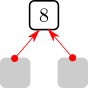
\includegraphics[width=2cm]{cherry1a}
  \end{tabular}
\end{center}
\end{nfig}
  \item By stringing such little ``cherries'' together we can describe more
complicated formulas. For example, if we compute ``$(3+5)\times 2$'', we first
compute ``$(3+5)$'' and then multiply the result by 2. The corresponding
diagrams are
\end{itemize}
\begin{wfig}
\begin{center}
  \begin{tabular}{m{3cm} c m{3cm} c m{3cm}}
 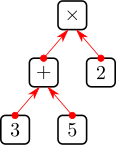
\includegraphics[width=3cm]{cherry2}
  & \text{ evaluates to }
  & \includegraphics[width=3cm]{cherry2a}
  & \text{ evaluates to }
  & \includegraphics[width=3cm]{cherry2b}
  \end{tabular}
\end{center}
\end{wfig}

The tree we drew in Figure~\ref{fig tree rational} above representing our formula has $x$
in some of the boxes,
and so when we want to compute the function at a particular value of $x$ --- say
at $x=5$ --- then we replace those ``$x$''s in the tree by that value and then
compute back up the tree. See the example below
\begin{fig}
\begin{center}
\begin{tabular}{c m{55mm} c m{55mm} c}
  Start
  & 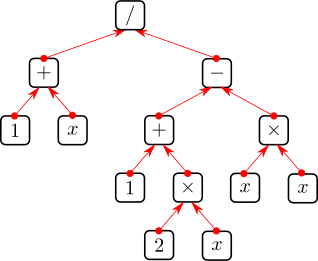
\includegraphics[width=50mm]{tree1b}
  & $\mapsto$
  & \includegraphics[width=50mm]{tree1b2}
  &
  \\[15ex]
  $\mapsto$
  & \includegraphics[width=50mm]{tree1b3}
  & $\mapsto$
  & 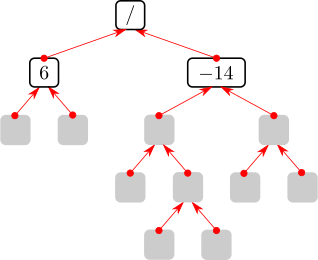
\includegraphics[width=50mm]{tree1b4}
  & \\[15ex]
  $\mapsto$
  & \includegraphics[width=50mm]{tree1b5}
  & & and we are done.
\end{tabular}
\end{center}
\end{fig}

This is not the only parse tree associated with the formula for $f(x)$; we
could also decompose it as
\begin{fig}
\begin{center}
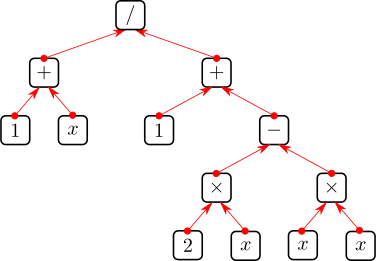
\includegraphics[height=5cm]{tree1a}
\end{center}
\end{fig}
We are able to do this because when we compute the denominator $1+2x-x^2$, we
can compute it as
\begin{align*}
  1+2x-x^2 &= \text{ either } (1+2x)-x^2 \text{ or } = 1 + (2x-x^2).
\end{align*}
Both\footnote{We could also use, for example, $1+2x-x^2 = (1-x^2)+2x$.} are
correct because addition is ``associative''. Namely
\begin{align*}
  a+b+c &= (a+b)+c = a+(b+c).
\end{align*}
Multiplication is also associative:
\begin{align*}
  a \times b \times c &= (a \times b) \times c = a \times (b \times c).
\end{align*}

\begin{eg}[parsing a formula]
Consider the formula
  \begin{align*}
  g(t) &= \left(\frac{t+\pi}{t-\pi} \right) \cdot \sin\left( \frac{t+\pi}{2}
\right).
\end{align*}
  This introduces a new idea --- we have to evaluate $\frac{t+\pi}{2}$ and then
compute the sine of that number. The corresponding tree can be written as
\begin{efig}
\begin{center}
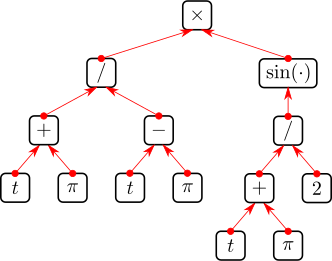
\includegraphics[height=5cm]{tree2}
\end{center}
\end{efig}
  If we want to evaluate this at $t = \pi/2$ then we get the following\dots
\begin{wfig}
\begin{center}
\begin{tabular}{c m{58mm} c m{58mm} c}
  Start
  & \includegraphics[width=55mm]{tree2a}
  & $\mapsto$
  & 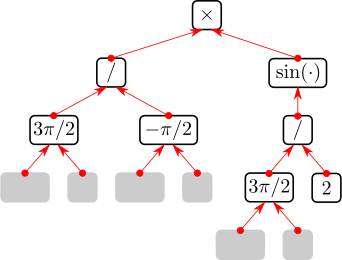
\includegraphics[width=55mm]{tree2b}
  &
  \\[15ex]
  $\mapsto$
  & \includegraphics[width=55mm]{tree2c}
  & $\mapsto$
  & \includegraphics[width=55mm]{tree2d}
  & \\[15ex]
  $\mapsto$
  & \includegraphics[width=55mm]{tree2e}
  & & and we are done.
\end{tabular}
\end{center}
\end{wfig}

\end{eg}

% \begin{eg}
%  And another one\dots
% \begin{align*}
%   \text{We need another nice example in here.}
% \end{align*}
% \end{eg}

It is highly unlikely that you will ever need to explicitly construct such a
tree for any problem in the remainder of the text. The main point of
introducing these objects and working through a few examples is to realise that
all the functions that we will examine are constructed from simpler pieces. In
particular we have constructed all the above examples from simple ``building
blocks''
\begin{itemize}
 \item constants --- fixed numbers like $1, \pi$ and so forth
 \item variables --- usually $x$ or $t$, but sometimes other symbols
 \item standard functions --- like trigonometric functions (sine, cosine and
tangent), exponentials and logarithms.
\end{itemize}
These simple building blocks are combined using arithmetic
\begin{itemize}
 \item addition and subtraction --- $a + b$ and $a-b$
\item multiplication and division --- $a \cdot b$ and $\nicefrac{a}{b}$
\item raising to a power --- $a^n$
\item composition --- given two functions $f(x)$ and $g(x)$ we form a
new function $f(g(x))$ by evaluating $y=g(x)$ and then evaluating $f(y) =
f(g(x))$.
\end{itemize}
During the rest of the course when we learn how to compute limits and
derivatives, our computations require us to understand the way we construct
functions as we have just described.

That is, in order to compute the derivative\footnote{We get to this in Chapter~\ref{chap
deriv} --- don't worry about exactly what it is just now.} of a function we
have to see how to construct the function from these building blocks (i.e. the
constants, variables and standard functions) using arithmetic operations. We
will then construct the derivative by following these same steps. There will be
simple rules for finding the derivatives of the simpler pieces and then rules
for putting them together following the arithmetic used to construct the function.


\section{Inverse Functions}\label{sec inverse functions}
There is one last thing that we should review before we get into the main material of the
course and that is inverse functions. As we have seen above functions are really just
rules for taking an input (almost always a number), processing it somehow (usually by a
formula) and then returning an output (again, almost always a number).
\begin{align*}
 \text{input number $x$} \quad \mapsto \quad \text{$f$ does ``stuff'' to $x$} \quad
\mapsto \quad \text{return number $y$}
\end{align*}
In many situations it will turn out to be very useful if we can undo whatever it is that
our function has done. ie
\begin{align*}
 \text{take output $y$} \quad \mapsto \quad \text{do ``stuff'' to $y$}
  \quad \mapsto \quad \text{return the original $x$}
\end{align*}
When it exists, the function ``which undoes'' the function $f(x)$ is found by solving
$y=f(x)$ for $x$ as a function of $y$ and is called the inverse function of $f$.
It turns out that it is not always possible to solve $y=f(x)$ for $x$ as a
function of $y$. Even when it is possible, it can be really hard to
do\footnote{Indeed much of encryption exploits the fact that you can find
functions that are very quick to do, but very hard to undo. For example --- it
is very fast to multiply two large prime numbers together, but very hard to take
that result and factor it back into the original two primes. The interested
reader should look up trapdoor functions.}.


For example --- a particle's position, $s$, at time $t$ is given by the formula
$s(t) = 7t$ (sketched below). Given a calculator, and any particular number $t$,
you can quickly work out the corresponding positions $s$. However, if you are
asked the question ``When does the particle reach $s=4$?'' then to answer it we
need to be able to ``undo'' $s(t)=4$ to isolate $t$. In this case, because
$s(t)$ is always increasing, we can always undo $s(t)$ to get a unique answer:
\begin{align*}
  s(t) &= 7t = 4 & \text{ if and only if }&& t&= \frac{4}{7}.
\end{align*}

However, this question is not always so easy. Consider the sketch of $y=\sin(x)$
below; when is $y=\half$? That is, for which values $x$ is $\sin(x)=\half$? To
rephrase it again, at which values of $x$ does the curve $y=\sin x$ (which is
sketched in the right
half of Figure~\ref{fig inv1}) cross the horizontal straight line $y=\frac{1}{2}$ (which
is also sketched in the same figure)?
\begin{fig}\label{fig inv1}
\begin{center}
 \includegraphics[height=5cm]{inv1}
\end{center}
\end{fig}
We can see that there are going to be an infinite number of $x$-values that give
$y=\sin(x)=\half$; there is no unique answer.

Recall (from Definition~\ref{def function}) that for any given input, a function must
give a unique output. So if we want to find a \emph{function} that undoes $s(t)$, then
things are good --- because each $s$-value corresponds to a unique $t$-value. On the
other hand, the situation with $y=\sin x$ is problematic --- any given $y$-value is
mapped to by many different $x$-values. So when we look for an \emph{unique} answer to
the question ``When is $\sin x = \half$?'' we cannot answer it.

This ``uniqueness'' condition can be made more precise:
\begin{defn}
 A function $f$ is one-to-one (injective) when it never takes the same $y$
value more than once. That is
\begin{align*}
  \mbox{if } x_1 \neq x_2 \mbox{ then } f(x_1) \neq f(x_2)
\end{align*}
\end{defn}
There is an easy way to test this when you have a plot of the function --- the
horizontal line test.
\begin{defn}[Horizontal line test]
 A function is one-to-one if and only if no horizontal line $y=c$ intersects
the graph $y=f(x)$ more than once.
\end{defn}
\noindent i.e. every horizontal line intersects the graph either zero or
one times. Never twice or more. This test tell us that $y=x^3$ is
one-to-one, but $y=x^2$ is not. However note that if we restrict the domain of
$y=x^2$ to $x \geq 0$ then the horizontal line test is passed. This is one of
the reasons we have to be careful to consider the domain of the function.
\begin{fig}
\begin{center}
 \includegraphics[height=3.5cm]{inv1A}
\end{center}
\end{fig}

When a function is one-to-one then it has an inverse function.
\begin{defn}\label{def inv func}
 Let $f$ be a one-to-one function with domain $A$ and range $B$. Then its inverse
function is denoted $f^{-1}$ and has domain $B$ and range $A$. It is defined by
\begin{align*}
  f^{-1}(y) &= x & \text{ whenever }&& f(x)&=y
\end{align*}
for any $y \in B$.
\begin{efig}
\begin{center}
 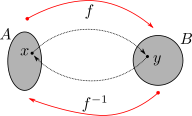
\includegraphics[height=4cm]{inv2}
\end{center}
\end{efig}
\end{defn}
So if $f$ maps $x$ to $y$, then $f^{-1}$ maps $y$ back to $x$. That is $f^{-1}$ ``undoes''
$f$. Because of this we have
\begin{align*}
  f^{-1}( f(x) ) &= x  &\mbox{ for any $x \in A$}\\
   f( f^{-1}(y) )&=y &\mbox{ for any $y \in B$}
\end{align*}
We have to be careful not to confuse $f^{-1}(x)$ with $\ds \frac{1}{f(x)}$. The ``$-1$''
is not an exponent.

\begin{eg}
Let $f(x)=x^5+3$ on domain $\mathbb{R}$. To find its inverse we do the following
\begin{itemize}
 \item Write $y=f(x)$; that is $y=x^5+3$.
 \item Solve for $x$ in terms of $y$ (this is not always easy) --- $x^5=y-3$, so
$x=(y-3)^{1/5}$.
\item The solution is $f^{-1}(y) = (y-3)^{1/5}$.
\item Recall that the ``$y$'' in $f^{-1}(y)$ is a dummy variable. That is,
$f^{-1}(y) = (y-3)^{1/5}$ means that if you feed the number $y$ into the function
$f^{-1}$ it outputs the number $(y-3)^{1/5}$. You may call the input variable anything
you like. So if you wish to call the input variable ``$x$'' instead of ``$y$'' then just
replace every $y$ in $f^{-1}(y)$ with an $x$.
\item That is $f^{-1}(x) = (x-3)^{1/5}$.
%  \item Then interchange $x \leftrightarrow y$ to get $f^{-1}(x)=y=(x-3)^{1/5}$.
\end{itemize}
\end{eg}


\begin{eg}
Let $g(x) = \sqrt{x-1}$ on the domain $x \geq 1$. We can find the inverse in the same way:
\begin{align*}
  y &= \sqrt{x-1} \\
  y^2 &= x-1 \\
  x &= y^2+1 = f^{-1}(y) & \text{or, writing input variable as ``$x$'':} \\
  f^{-1}(x) &= x^2+1.
\end{align*}
\end{eg}

Let us now turn to finding the inverse of $\sin(x)$ --- it is a little more tricky and we
have to think carefully about domains.


\begin{eg}
We have seen (back in Figure~\ref{fig inv1}) that $\sin(x)$ takes each value $y$
between $-1$ and $+1$ for infinitely many different values of $x$ (see
the left-hand graph in the figure below). Consequently $\sin(x)$, with domain
$-\infty <x <\infty$ does not have an inverse function.
\begin{wfig}
\begin{center}
 \includegraphics[height=4cm]{inv2B}
\end{center}
\end{wfig}
But notice that as $x$ runs from $-\frac{\pi}{2}$ to $+\frac{\pi}{2}$, $\sin(x)$ increases
from $-1$ to $+1$. (See the middle graph in the figure above.) In particular, $\sin(x)$
takes each value $-1 \le y\le 1$ for exactly one $-\frac{\pi}{2}\le x\le \frac{\pi}{2}$.
So if we restrict $\sin x$ to have domain $-\frac{\pi}{2}\le x\le \frac{\pi}{2}$, it does
have an inverse function, which is traditionally called arcsine (see Appendix~\ref{sec
inv trig}).

That is, by definition, for each $-1\le y\le 1$, $\arcsin(y)$ is the unique
$-\frac{\pi}{2}\le x\le \frac{\pi}{2}$ obeying $\sin(x)=y$. Equivalently, exchanging the
dummy variables x and y throughout the last sentence gives that for each $-1\le
x\le 1$, $\arcsin(x)$ is the unique $-\frac{\pi}{2}\le y\le \frac{\pi}{2}$
obeying $\sin(y)=x$.
\end{eg}



It is an easy matter to construct the graph of an inverse function
from the graph of the original function. We just need to remember that
\begin{equation*}
Y=f^{-1}(X)  \iff f(Y)=X
\end{equation*}
which is $y=f(x)$ with $x$ renamed to $Y$ and $y$ renamed to $X$.
%Each point on the graph of $f$ has coordinates $\big(x\,,\,f(x)\big)$.
%If we rename $x$ to $Y$, those coordinates become
%\begin{equation*}
%\big(Y,f(Y)\big) = \big(f^{-1}(X),X\big) = (Y,X)\quad\text{with}\quad Y=f^{-1}(X)
%\end{equation*}
%To get the graph of $f^{-1}$ we just need to reinterpret these statements
%graphically.

 Start by drawing the graph of $f$, labelling the $x$-- and $y$--axes
and labelling the curve $y=f(x)$.
\begin{efig}
\begin{center}
   
\includegraphics{fInvA}
\end{center}
\end{efig}
Now replace each $x$ by $Y$ and each $y$ by $X$  and replace the resulting
label $X=f(Y)$ on the curve by the equivalent $Y=f^{-1}(X)$.
\begin{efig}
\begin{center}
   
\includegraphics{fInvB}
\end{center}
\end{efig}
Finally we just need to redraw the sketch with the $Y$ axis running vertically
(with $Y$ increasing upwards) and the $X$ axis running horizontally (with
$X$ increasing to the right). To do so, pretend that the sketch is on
a transparency or on a very thin piece of paper that you can see through.
Lift the sketch up and flip it over so that the $Y$ axis runs vertically
and the $X$ axis runs horizontally. If you want, you can also convert the upper
case $X$ into a lower case $x$ and the upper case $Y$ into a lower case
$y$.
\begin{wfig}
\begin{center}
   \includegraphics{fInvC}\qquad   
\includegraphics{fInvD}
\end{center}
\end{wfig}
Another way to say ``flip the sketch over so as to exchange the
$x$-- and $y$--axes'' is ``reflect in the line $y=x$''. In the
figure below the blue ``horizontal'' elliptical disk that is centred
on $(a,b)$ has been reflected in the line $y=x$ to give the red ``vertical''
elliptical disk centred on $(b,a)$.
\begin{wfig}
\begin{center}
   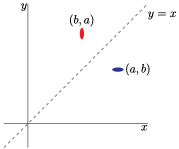
\includegraphics{fInvR}
\end{center}
\end{wfig}

\begin{eg}\label{eg:INVlogbaseten}
As an example, let $f(x) = x^2$ with domain $0\le x< \infty$.
\begin{itemize}\itemsep1pt \parskip0pt \parsep0pt \itemindent 10pt
\item
When $x=0$, $f(x)=0^2=0$.
\item
As $x$ increases, $x^2$ gets bigger and bigger.
\item
When $x$ is very large and positive,
$x^2$ is also very large and positive.
(For example, think $x=100$.)
\end{itemize}
The graph of $y=f(x)=x^2$ is the blue curve below.
By definition, $Y=f^{-1}(X)$ if $X=f(Y)=Y^2$. That is, if $Y=\sqrt{X}$.
(Remember that, to be in the domain of $f$, we must have $Y\ge 0$.)
So the inverse function of ``square'' is ``square root''. The
graph of $f^{-1}$ is the red curve below. The red curve is the
reflection of the blue curve in the line $y=x$.
\begin{wfig}
\begin{center}
   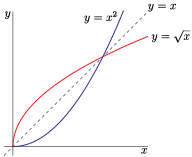
\includegraphics{fInvSqA}
\end{center}
\end{wfig}
\end{eg}

% %
% Copyright 2018 Joel Feldman, Andrew Rechnitzer and Elyse Yeager.
% This work is licensed under a Creative Commons Attribution-NonCommercial-ShareAlike 4.0 International License.
% https://creativecommons.org/licenses/by-nc-sa/4.0/
%
\graphicspath{{./figures/limits/}}
%%%%%%%%%


\chapter{Limits}\label{chap limits}

So very roughly speaking, ``Differential Calculus'' is the study of how a
function changes as its input changes. The mathematical object we use to
describe this is the ``derivative'' of a function. To properly describe what
this thing is we need some machinery; in particular we need to define what we
mean by ``tangent'' and ``limit''. We'll get back to defining the derivative in
Chapter~2.

\section{Drawing Tangents and a First Limit}\label{sec first lim}
Our motivation for developing ``limit'' --- being the title and subject of this
chapter --- is going to be two related problems of drawing tangent lines and
computing velocity.

Now --- our treatment of limits is not going to be completely mathematically
rigorous, so we won't have too many formal definitions. There will be a few
mathematically precise definitions and theorems as we go, but we'll make sure
there is plenty of explanation around them.

Let us start with the ``tangent line'' problem. Of course, we need to define
``tangent'', but we won't do this formally. Instead let us draw some pictures.
\begin{fig}
\begin{center}
 \includegraphics[height=4cm]{tang1}
\end{center}
\end{fig}
Here we have drawn two very rough sketches of the curve $y=x^2$ for $x \geq 0$.
These are not very good sketches for a couple of reasons
\begin{itemize}
 \item The curve in the figure does not pass through $(0,0)$, even though
$(0,0)$ lies on $y=x^2$.
 \item The top-right end of the curve doubles back on itself and so fails the
vertical line test  that all functions must satisfy\footnote{Take a moment to
go back and reread Definition~\ref{def function}.} --- for each $x$-value there
is exactly one $y$-value for which $(x,y)$ lies on the curve $y=x^2$.
\end{itemize}
So let's draw those more carefully.
\begin{fig}
\begin{center}
 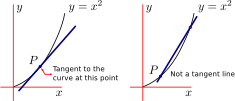
\includegraphics[height=4cm]{tang1a}
\end{center}
{Sketches of the curve $y=x^2$. (left) shows a tangent line, while
(right) shows a line that is not a tangent.}
\label{fig tang1a}
\end{fig}
These are better. In both cases we have drawn $y=x^2$ (carefully) and then
picked a point on the curve --- call it $P$. Let us zoom in on the ``good''
example:
\begin{fig}
\begin{center}
 \includegraphics[height=4cm]{tang1aa}
\end{center}
We see that, the more we zoom in on the point $P$, the more the graph of the function
(drawn in black) looks like a straight line --- that line is the tangent line (drawn in
blue).
\label{fig tang1aa}
\end{fig}
We see that as we zoom in on the point $P$, the graph of the function looks
more and more like a straight line. If we kept on zooming in on $P$ then the
graph of the function would be indistinguishable from a straight line. That
line is the tangent line (which we have drawn in blue). A little more
precisely, the blue line is ``the tangent line to the function at $P$''. We
have to be a little careful, because if we zoom in at a different point, then
we will find a different tangent line.

Now lets zoom in on the ``bad'' example we see that the blue line looks very
different from the function; because of this, the blue line is not the tangent
line at $P$.
\begin{fig}
\begin{center}
 \includegraphics[height=4cm]{tang1ab}
\end{center}
Zooming in on $P$ we see that the function (drawn in black) looks more
and more like a straight line --- however it is not the same line as that drawn
in blue. Because of this the blue line is not the tangent line.
\label{fig tang1ab}
\end{fig}

Here are a couple more examples of tangent lines
\begin{fig}
\begin{center}
 \includegraphics[height=4cm]{tang1b}
\end{center}
More examples of tangent lines.
\label{fig tang1b}
\end{fig}
The one on the left is very similar to the good example on $y=x^2$ that we saw
above, while the one on the right is different --- it looks a little like the
``bad'' example, in that it crosses our function the curve at some distant
point. Why is the line in Figure~\ref{fig tang1b}(right) a tangent while the
line in Figure~\ref{fig tang1a}(right) not a tangent? To see why, we should
again zoom in close to the point where we are trying to draw the tangent.
\begin{fig}
\begin{center}
 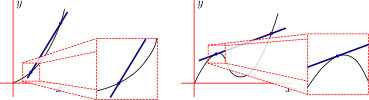
\includegraphics[height=4cm]{tang1c}
\end{center}
\end{fig}
As we saw above in Figure~\ref{fig tang1ab}, when we zoom in around our example
of ``not a tangent line'' we see that the straight line looks very different
from the curve at the ``point of tangency'' --- i.e. where we are trying to draw
the tangent. The line drawn in Figure~\ref{fig tang1b}(right) looks more and
more like the function as we zoom in.

This example raises an important point --- when we are trying to draw a
tangent line, we don't care what the function does a long way from the
point; the tangent line to the curve at a particular point $P$, depends only on
what the function looks like close to that point $P$.

To illustrate this consider the sketch of the function $y = \sin(x)$ and its
tangent line at~$(x,y)=(0,0)$:
\begin{fig}
\begin{center}
 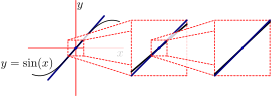
\includegraphics[height=4cm]{tang1d}
\end{center}
\end{fig}
As we zoom in, the graph of $\sin(x)$ looks more and more like a straight line
--- in fact it looks more and more like the line $y=x$. We have also sketched
this tangent line. What makes this example a little odd is that the tangent
line crosses the function. In the examples above, our tangent lines just
``kissed'' the curve and did not cross it (or at least did not cross it
nearby).

Using this idea of zooming in at a particular point, drawing a tangent line is
not too hard. However,  finding the equation of the tangent line presents us
with a few challenges. Rather than leaping into the general  theory, let us do a
specific example. Let us find the the equation of the tangent line to the curve
$y=x^2$ at the point $P$ with coordinates\footnote{
Note that the \emph{coordinates} $(x,y)$ is an ordered pair of two numbers $x$
and $y$. Traditionally the first number is called the \emph{abscissa} while the
second is the \emph{ordinate}, but these terms are a little archaic. It is now
much more common to hear people refer to the first number as
the \emph{$x$-coordinate} and the second as \emph{$y$-coordinate}.}
$(x,y)=(1,1)$.

To find the equation of a line we either need
\begin{itemize}
 \item the slope of the line and a point on the line, or
 \item two points on the line, from which we can compute the slope via the
formula
\begin{align*}
  m &= \frac{y_2 - y_1}{x_2 - x_1}
\end{align*}
\end{itemize}
and then write down the equation for the line via a formula such as
\begin{align*}
  y &= m \cdot(x - x_1) + y_1.
\end{align*}


We cannot use the first method because we do not know what the slope of the
tangent line should be. To work out the slope we need calculus --- so we'll
be able to use this method once we get to the next chapter on
``differentiation''.

It is not immediately obvious how we can use the second method, since we only
have one point on the curve, namely $(1,1)$. However we can use it to ``sneak
up'' on the answer.  Let's approximate the tangent line, by drawing a line that
passes through $(1,1)$ and some nearby point --- call it $Q$. Here is our
recipe:
\begin{itemize}
 \item We are given the point $P=(1,1)$ and we are told
\begin{quote}
Find the tangent line to the curve $y=x^2$ that passes through $P = (1,1)$.
\end{quote}
 \item We don't quite know how to find a line given just 1 point, however we do
know how to find a line passing through 2 points. So pick another point on the
curves whose coordinates are very close to $P$. Now rather than picking some
actual numbers, I am going to write our second point as $Q = (1+h, (1+h)^2)$.
That is, a point $Q$ whose $x$-coordinate is equal to that of $P$ plus a little
bit --- where the little bit is some small number $h$.  And since this point
lies on the curve $y=x^2$, and $Q$'s x-coordinate is $1+h$, $Q$'s y-coordinate must
be $(1+h)^2$.

If having $h$ as an variable rather than a number bothers you, start by
thinking of $h$ as~$0.1$.

 \item A picture of the situation will help.
\end{itemize}
\begin{fig}
  \begin{center}
  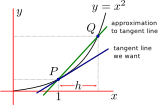
\includegraphics[height=5cm]{tang2}
  \end{center}
\end{fig}
\begin{itemize}
  \item This line that passes through the curve in two places $P$ and $Q$ is
  called a ``secant line''.

  \item The slope of the line is then
\begin{align*}
  m &= \frac{y_2 - y_1}{x_2-x_1} \\
  &= \frac{(1+h)^2-1}{(1+h)-1}
  =  \frac{1+2h+h^2-1}{h}
  = \frac{2h+h^2}{h}
  = 2+h
\end{align*}
  where we have expanded $(1+h)^2 = 1+2h+h^2$ and then cleaned up a bit.
\end{itemize}
Now this isn't our tangent line because it passes through 2 nearby points on
the curve --- however it is a reasonable approximation of it. Now we can make
that approximation better and so ``sneak up'' on the tangent line by considering
what happens when we move this point $Q$ closer and closer to $P$. i.e. make the
number $h$ closer and closer to zero.
\begin{fig}
\begin{center}
  \includegraphics[width=\textwidth]{tang2a}
\end{center}
\end{fig}

First look at the picture. The original choice of $Q$ is on the left, while on
the right we have drawn what happens if we choose $h'$ to be some number a
little smaller than $h$, so that our point $Q$ becomes a new point $Q'$ that is
a little closer to $P$. The new approximation is better than the first.

So as we make $h$ smaller and smaller, we bring $Q$ closer and closer to
$P$, and make our secant line a better and better approximation of the
tangent line. We can observe what happens to the slope of the line as we
make $h$ smaller by plugging some numbers into our formula $m=2+h$:
\begin{align*}
 h=0.1 && m = 2.1\\
 h=0.01 && m= 2.01 \\
 h=0.001 && m= 2.001.
\end{align*}
So again we see that as this difference in $x$ becomes smaller and smaller, the
slope appears to be getting closer and closer to $2$. We can write this more
mathematically as
\begin{align*}
 \lim_{h \to 0} \frac{(1+h)^2-1}{h} &= 2
 \end{align*}
This is read as
\begin{quote}
 The limit, as $h$ approaches $0$, of $\frac{(1+h)^2-1}{h}$ is $2$.
\end{quote}
This is our first limit! Notice that we can see this a little more clearly with a quick
bit of algebra:
\begin{align*}
\frac{(1+h)^2-1}{h} &= \frac{(1+2h+h^2)-1}{h} \\
  &= \frac{2h+h^2}{h} \\
  &= 2+h
\intertext{So it is not unreasonable to expect that}
\lim_{h \to 0} \frac{(1+h)^2-1}{h} &= \lim_{h \to 0} (2+h) = 2.
\end{align*}


Our tangent line can be thought of as the end of this process --- namely as we
bring $Q$ closer and closer to $P$, the slope of the secant line comes
closer and closer to that of the tangent line we want. Since we have worked out
what the slope is --- that is the limit we saw just above --- we now know
the slope of the tangent line is $2$. Given this, we can work out the
equation for the tangent line.
\begin{itemize}
 \item The equation for the line is $y=mx+c$. We have 2 unknowns $m$ and $c$ ---
so we need 2 pieces of information to find them.
 \item Since the line is tangent to $P = (1,1)$ we know the line must pass
through $(1,1)$. From the limit we computed above, we also know that the line
has slope $2$.
 \item Since the slope is $2$ we know that $m=2$. Thus the equation of the line
is $y=2x+c$.
 \item We know that the line passes through $(1, 1)$, so that $y=2x+c$ must be $1$
  when $x=1$. So $1 = 2 \cdot 1 + c$, which forces $c = -1$.
\end{itemize}
So our tangent line is $y=2x-1$.

\section{Another Limit and Computing Velocity} \label{sec velocity}
Computing tangent lines is all very well, but what does this have to do with
applications or the ``Real World''? Well - at least initially our use of limits
(and indeed of calculus) is going to be a little removed from real world
applications. However as we go further and learn more about limits and
derivatives we will be able to get closer to real problems and their solutions.

So stepping just a little closer to the real world, consider the following
problem. You drop a ball from the top of a very very tall building. Let $t$ be
elapsed time measured in seconds, and $s(t)$ be the distance the ball has fallen
in metres. So $s(0) = 0$.

\emph{Quick aside:} there is quite a bit going on in the statement of this
problem. We have described the general picture --- tall building, ball, falling
--- but we have also introduced notation, variables and units. These will be
common first steps in applications and are necessary in order to translate a
real world problem into mathematics in a clear and consistent way.


Galileo\footnote{Perhaps one of the most famous experiments in all of physics
is Galileo's leaning tower of Pisa experiment, in which he dropped two balls
of different masses from the top of the tower and observed that the time
taken to reach the ground was independent of their mass. This
disproved Aristotle's assertion that heavier objects fall faster. It is quite
likely that Galileo did not actually perform this experiment. Rather it was a
thought-experiment. However a quick glance at Wikipedia will turn up some
wonderful footage from the Apollo 15 mission showing a hammer and feather being
dropped from equal height hitting the moon's surface at the same time.
Finally, Galileo determined that the speed of falling objects increases at a
constant rate, which is equivalent to the formula stated here, but it is
unlikely that he wrote down an equation exactly as it is here.}
worked out that $s(t)$ is a quadratic function:
\begin{align*}
  s(t) &= 4.9 t^2.
\end{align*}
The question that is posed is
\begin{quote}
 How fast is the ball falling after 1 second?
\end{quote}

Now before we get to answering this question, we should first be a little more
precise. The wording of this question is pretty sloppy for a couple of reasons:
\begin{itemize}
 \item What we do mean by  ``after 1 second''? We know the ball
will move faster and faster as time passes, so after 1 second it does not fall
at one fixed speed.
 \item As it stands a reasonable answer to the question would be just ``really
fast''. If the person asking the question wants a numerical answer it
would be better to ask ``At what speed'' or ``With what velocity''.
\end{itemize}
We should also be careful using the words ``speed'' and ``velocity'' --- they
are not interchangeable.
\begin{itemize}
 \item Speed means the distance travelled per unit time and is always a
non-negative number. An unmoving object has speed $0$, while a moving object has
positive speed.
 \item Velocity, on the other hand, also specifies the direction of motion.
In this text we will almost exclusively deal with objects moving along
straight lines. Because of this velocities will be positive or negative
numbers indicating  which direction the object is moving along the line. We
will be more precise about this later\footnote{Getting the sign of velocity
wrong is a very common error --- you should be careful with it.}.
\end{itemize}
A better question is
\begin{quote}
 What is the velocity of the ball precisely 1 second after it is dropped?
\end{quote}
or even better:
\begin{quote}
 What is the velocity of the ball at the 1 second mark?
\end{quote}
This makes it very clear that we want to know what is happening at exactly 1
second after the ball is dropped.

There is something a little subtle going on in this question. In particular,
what do we mean by the velocity at $t=1$?. Surely if we freeze time at $t=1$
second, then the object is not moving at all? This is definitely \emph{not}
what we mean.

If an object is moving at a constant velocity\footnote{Newton's first law of
motion states that an object in motion moves with constant velocity unless a
force acts on it --- for example gravity or friction.} in the positive
direction, then that velocity is just the distance travelled divided by the time
taken. That is
\begin{align*}
  v &= \frac{\text{distance moved}}{\text{time taken}}
\end{align*}
An object moving at constant velocity that moves $27$ metres in $3$ seconds has
velocity
\begin{align*}
  v &= \frac{27 m}{3 s} = 9 m/s.
\end{align*}
When velocity is constant everything is easy.

However, in our falling object example, the object is being acted on by
gravity and its speed is definitely not constant. Instead of asking for
\emph{THE} velocity, let us examine the ``average velocity'' of the object over
a certain window of time. In this case the formula is very similar
\begin{align*}
  \text{average velocity } &= \frac{\text{distance moved}}{\text{time taken}}
\end{align*}
But now I want to be more precise, instead write
\begin{align*}
  \text{average velocity } &= \frac{\text{difference in
distance}}{\text{difference in time}}
\end{align*}
Now in spoken English we haven't really changed much --- the distance moved is
the difference in position, and the time taken is just the difference in time
--- but the latter is more mathematically precise, and is easy to translate
into the following equation
\begin{align*}
  \text{average velocity } &= \frac{s(t_2) - s(t_1)}{t_2 - t_1}.
\end{align*}
This is the formula for the average velocity of our object between time $t_1$
and $t_2$. The denominator is just the difference between these times and the
numerator is the difference in position --- i.e. position at time $t_1$ is just
$s(t_1)$ and position at time $t_2$ is just $s(t_2)$.


So what is the average velocity of the falling ball between $1$ and $1.1$
seconds? All we need to do now is plug some numbers into our formula
\begin{align*}
  \mbox{average velocity} &= \frac{\mbox{difference in
position}}{\mbox{difference in time}} \\
  &= \frac{s(1.1) - s(1)}{1.1-1} \\
  &= \frac{4.9 (1.1)^2 - 4.9(1)}{0.1} = \frac{4.9 \times 0.21}{0.1} = 10.29 m/s
\end{align*}
And we have our average velocity. However there is something we should notice
about this formula and it is easier to see if we sketch a graph of the function
$s(t)$
\begin{fig}
\begin{center}
 \includegraphics[width=\textwidth]{vel1}
\end{center}
\end{fig}
So on the left I have drawn the graph and noted the times $t=1$ and $t=1.1$.
The
corresponding positions on the axes and the two points on the curve.  On the
right I have added a few more details. In particular I have noted the
differences in position and time, and the line joining the two points. Notice
that the slope of this line is
\begin{align*}
  \text{slope} &= \frac{\text{change in $y$}}{\text{change in $x$}}
  = \frac{\text{difference in $s$}}{\text{difference in $t$}}
\end{align*}
which is precisely our expression for the average velocity.

Let us examine what happens to the average velocity as we look over smaller and
smaller time-windows.
\begin{align*}
  \text{time window} && \text{average velocity}\\
  1 \leq t \leq 1.1 && 10.29 \\
  1 \leq t \leq 1.01 && 9.849 \\
  1 \leq t \leq 1.001 && 9.8049 \\
  1 \leq t \leq 1.0001 && 9.80049
\end{align*}
As we make the time interval smaller and smaller we find that the average
velocity is getting closer and closer to $9.8$. We can be a little more precise
by finding the average velocity between $t=1$ and $t=1+h$ --- this is very
similar to what we did for tangent lines.
\begin{align*}
  \text{average velocity} &= \frac{s(1+h) - s(1)}{(1+h)-1} \\
  &= \frac{4.9(1+h)^2 - 4.9}{h} \\
  &= \frac{9.8h + 4.9h^2}{h} \\
  &= 9.8 + 4.9h
\end{align*}
Now as we squeeze this window between $t=1$ and $t=1+h$ down towards zero, the
average velocity becomes the ``instantaneous velocity'' --- just as the
slope of the secant line becomes the slope of the tangent line. This is
our second limit
\begin{align*}
 v(1) &= \lim_{h \to 0} \frac{s(1+h)-s(1)}{h} = 9.8
\end{align*}
More generally we define the instantaneous velocity at time $t=a$ to be the
limit
\begin{align*}
  v(a) &= \lim_{h \to 0} \frac{ s(a+h) - s(a) }{h}
\end{align*}
We read this as
\begin{quote}
 The velocity at time $a$ is equal to the limit as $h$ goes to zero of
$\frac{s(a+h)-s(a)}{h}$.
\end{quote}

While we have solved the problem stated at the start of this section, it is
clear that if we wish to solve similar problems that we will need to
understand limits in a more general and systematic way.

\section{The Limit of a Function}
\label{sec lim func}

Before we come to definitions, let us start with a little notation for limits.
\begin{notn}\label{ntn_1_3_1}
We will often write
\begin{align*}
  \lim_{x \to a} f(x) = L
\end{align*}
which should be read as
\begin{quote}
The limit of $f(x)$ as $x$ approaches $a$ is $L$.
\end{quote}
\end{notn}
The notation is just shorthand --- we don't want to have to write out long
sentences as we do our mathematics. Whenever you see these symbols you
should think of that sentence.

This shorthand also has the benefit of being mathematically precise (we'll see
this later), and (almost) independent of the language in which the author is
writing. A mathematician who does not speak English can read the above formula
and understand exactly what it means.

In mathematics, like most languages, there is usually more than one way of
writing things and we can also write the above limit as
\begin{align*}
  f(x) \to L \mbox{ as } x \to a
\end{align*}
This can also be read as above, but also as
\begin{quote}
  $f(x)$ goes to $L$ as $x$ goes to $a$
\end{quote}
They mean exactly the same thing in mathematics, even though they might be
written, read and said a little differently.


To arrive at the definition of limit, we want to start\footnote{Well, we
had two limits in the previous sections, so perhaps we really want to
``restart'' with a very simple example.} with a very simple example.

\begin{eg}\label{eg_1_3_1}
Consider the following function.
\begin{align*}
 f(x) &= \begin{cases}
          2x & x<3 \\
          9 & x=3 \\
          2x & x>3
         \end{cases}
\end{align*}
This is an example of a piece-wise function\footnote{We saw another
piecewise function back in Example~\ref{eg piecewise}.}. That is, a function
defined in several pieces, rather than as a single formula. We evaluate the
function at a particular value of $x$ on a case-by-case basis. Here is a sketch
of it
\begin{efig}
\begin{center}
 \includegraphics[height=35mm]{piecewise1}
\end{center}
\end{efig}
Notice the two circles in the plot. One is open, $\circ$ and the other is
closed $\bullet$.
\begin{itemize}
 \item A filled circle has quite a precise meaning --- a filled circle at
$(x,y)$ means that the function takes the value $f(x) = y$.
 \item An open circle is a little harder --- an open circle at $(3,6)$ means
that the point $(3,6)$ is not on the graph of $y=f(x)$, i.e. $f(3) \neq 6$.
We should only use the open circle where it is absolutely necessary in order to
avoid confusion.
\end{itemize}
% In the case of our function, for almost all values of $x$ the function is just
% the straight line $y=2x$ --- so we start by drawing that. However at $x=3$
% something different happens and we have $f(3)=9$ --- thus we put a filled
% circle at $(x,y)=(3,9)$. At this point our graph would look like the following
% sketch on the left.
% \begin{center}
%  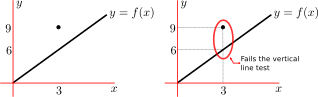
\includegraphics[height=4cm]{piecewise1a}
% \end{center}
% Unfortunately this is not the graph of a function, because it fails the
% vertical line test at $x=3$ --- it appears that $f(3)=9$ and $f(3)=6$ (see the
% sketch on the right). We fix this problem by using an open circle. We place the
% open circle at $(x,y)=(3,6)$ to show that the function is not the continuation
% of the straight line at this point and that in fact $f(3) \neq 6$.


This function is quite contrived, but it is a very good example to start
working with limits more systematically. Consider what the function does close
to $x=3$. We already know what happens exactly at $3$ --- $f(x)=9$ --- but I
want to look at how the function behaves very close to $x=3$. That is, what
does the function do as we look at a point $x$ that gets closer and closer to
$x=3$.

If we plug in some numbers very close to $3$ (but not exactly 3) into the
function we see the following:
\begin{center}
 \begin{tabular}{|c||c|c|c|c|c|c|c|}
  \hline
  $x$ & 2.9 & 2.99 & 2.999 & $\circ$ & 3.001 & 3.01 & 3.1\\
\hline
  $f(x)$ & 5.8 & 5.98 & 5.998 & $\circ$ & 6.002 & 6.02 & 6.2\\
\hline
 \end{tabular}
\end{center}
% \begin{align*}
%   x=2.9 && f(x) = 5.8 \\
%   x=2.99 && f(x) = 5.98 \\
%   x=2.999 && f(x) = 5.998 \\
%   x=3.1 && f(x) = 6.2 \\
%   x=3.01 && f(x) = 6.02 \\
%   x=3.001 && f(x) = 6.002
% \end{align*}
So as $x$ moves closer and closer to 3, without being exactly 3, we see that
the function moves closer and closer to 6. We can write this as
\begin{align*}
  \lim_{x \to 3} f(x) &= 6
\end{align*}
That is
\begin{quote}
 The limit as $x$ approaches $3$ of $f(x)$ is $6$.
\end{quote}
So for $x$ very close to $3$, without being exactly 3, the function is very close to $6$
--- which is a long way from the value of the function exactly at $3$, $f(3)=9$. Note
well that the behaviour of the function as $x$ gets very close to 3 \emph{does not}
depend on the value of the function \emph{at} 3.
\end{eg}

We now have enough to make an informal definition of a limit, which is actually
sufficient for most of what we will do in this text.
\begin{defn}[Informal definition of limit]\label{def_1_3_1}
  We write
\begin{align*}
  \lim_{x \to a} f(x) &= L
\end{align*}
% when the value of the function $f(x)$ gets closer and closer to $L$ as $x$
% gets closer and closer to $a$ (without\footnote{You may find the condition ``without
% being exactly $a$'' a little strange, but there is a good reason for it. One very
% important application of limits, indeed the main reason we teach the topic, is in
% the definition of derivatives (see Definition~\ref{def:DIFFderiv} in the next chapter).
% In that definition we need to compute the limit $\ds \lim_{x\rightarrow
% a}\frac{f(x)-f(a)}{x-a}$. In this case the function whose limit is being taken, namely
% $\frac{f(x)-f(a)}{x-a}$, is not defined at all at $x=a$.} being exactly $a$).
 if the value of the function $f(x)$ is sure to be arbitrarily close to $L$ whenever the value of $x$ is close enough to $a$, without\footnote{You may find the condition ``without  being exactly $a$'' a little strange, but there is a good reason for it. One very  important application of limits, indeed the main reason we teach the topic, is in the definition of derivatives (see Definition~\ref{def:DIFFderiv} in the next chapter).  In that definition we need to compute the limit $\ds \lim_{x\rightarrow a}\frac{f(x)-f(a)}{x-a}$. In this case the function whose limit is being taken, namely  $\frac{f(x)-f(a)}{x-a}$, is not defined at all at $x=a$.} being exactly $a$.
\end{defn}
In order to make this definition more mathematically correct, we need to
make the idea of ``closer and closer'' more precise --- we do this in
Section~\ref{sec opt formal limit}. It should be emphasised that the
formal definition and the contents of that section are optional
material.

For now, let us use the above definition to examine a more substantial
example.
\begin{eg}\label{eg_1_3_2}
Let $f(x) = \frac{x-2}{x^2+x-6}$ and consider its limit as $x \to 2$.


\begin{itemize}
 \item We are really being asked
  \begin{align*}
    \lim_{x \to 2} \frac{x-2}{x^2+x-6} &= \text{ what?}
  \end{align*}
  \item Now if we try to compute $f(2)$ we get $0/0$ which is
undefined. The function is not defined at that point --- this is a good example
of why we need limits.  We have to sneak up on these places where a function is
not defined (or is badly behaved).

 \item \textbf{VERY IMPORTANT POINT:} the fraction $\frac{0}{0}$ is
\emph{not} $\infty$ and it is not $1$, it is not defined. We cannot ever divide
by zero in normal arithmetic and obtain a consistent and mathematically
sensible answer. If you learned otherwise in high-school, you should quickly
unlearn it.

\item Again, we can plug in some numbers close to $2$ and see what we find
\begin{center}
 \begin{tabular}{|c||c|c|c|c|c|c|c|}
  \hline
  $x$ & 1.9 & 1.99 & 1.999 & $\circ$ & 2.001 & 2.01 & 2.1 \\
  \hline
%   $f(x)$ & 0.2040816327 & 0.2004008016 &0.2000400080
%   & $\circ$ & 0.1999600080 & 0.1996007984 & 0.1960784314 \\
  $f(x)$ & 0.20408 & 0.20040 &0.20004
  & $\circ$ & 0.19996 & 0.19960 & 0.19608 \\
\hline
\end{tabular}
\end{center}
% \begin{align*}
%   x=1.9 && f(x) &= 0.2040816327 \\
%   x=1.99 && f(x) &=  0.2004008016 \\
%   x=1.999 && f(x) &= 0.2000400080 \\
%   x=2.1 && f(x) &= 0.1960784314 \\
%   x=2.01 && f(x) &= 0.1996007984 \\
%   x=2.001 && f(x) &= 0.1999600080
% \end{align*}
\item So it is reasonable to suppose that
\begin{align*}
 \lim_{x \to 2} \frac{x-2}{x^2+x-6} &= 0.2
\end{align*}
\end{itemize}

\end{eg}

The previous two examples are nicely behaved in that the limits we tried to
compute actually exist. We now turn to two nastier examples\footnote{Actually,
they are good examples, but the functions in them are nastier.} in which the
limits we are interested in do not exist.

\begin{eg}[A bad example]
\label{eg sinpix}
Consider the following function $f(x) = \sin( \pi /x )$. Find the limit as $x
\to 0$ of $f(x)$.

We should see something interesting happening close to $x=0$ because $f(x)$ is
undefined there. Using your favourite graph-plotting software you can see that
the graph looks roughly like
\begin{efig}
\begin{center}
 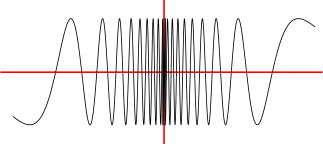
\includegraphics[height=4cm]{lim2}
\end{center}
\end{efig}
How to explain this? As $x$ gets closer and closer to zero, $\pi/x$ becomes
larger and larger (remember what the plot of $y=1/x$ looks like). So when you
take sine of that number, it oscillates faster and faster the closer you get to
zero. Since the function does not approach a single number as we bring $x$
closer and closer to zero, the limit does not exist.

We write this as
\begin{align*}
  \lim_{x\to 0} \sin \left(\frac{\pi}{x}\right) \text{ does not exist}
\end{align*}
It's not very inventive notation, however it is clear. We frequently
abbreviate ``does not exist'' to ``DNE'' and rewrite the above as
\begin{align*}
  \lim_{x\to 0} \sin \left(\frac{\pi}{x}\right) &= \text{DNE}
\end{align*}
\end{eg}

In the following example, the limit we are interested in does not exist.
However the way in which things go wrong is quite different from what we just
saw.
\begin{eg}\label{eg_1_3_3}
Consider the function
\begin{align*}
  f(x) &= \begin{cases}
           x & x<2 \\
           -1 & x=2 \\
           x+3 & x>2
          \end{cases}
\end{align*}
\begin{itemize}
 \item The plot of this function looks like this
\begin{efig}
\begin{center}
 \includegraphics[height=4cm]{lim1}
\end{center}
\end{efig}
\item So let us plug in numbers close to $2$.
\begin{center}
 \begin{tabular}{|c||c|c|c|c|c|c|c|}
  \hline
  $x$ & 1.9 & 1.99 & 1.999 & $\circ$ & 2.001 & 2.01 & 2.1 \\
\hline
  $f(x)$ & 1.9 & 1.99 & 1.999 & $\circ$ & 5.001 & 5.01 & 5.1 \\
\hline
  \end{tabular}
\end{center}
% \begin{align*}
%  x=1.9 && f(x) &= 1.9 \\
%  x=1.99 && f(x) &= 1.99 \\
%  x=1.999 && f(x) &= 1.999 \\
%  x=2.1 && f(x) &= 5.1\\
%  x=2.01 && f(x) &= 5.01\\
%  x=2.001 && f(x) &= 5.001
% \end{align*}
\item This isn't like before. Now when we approach from below, we seem to be
getting closer to $2$, but when we approach from above we seem to be getting
closer to $5$. Since we are not approaching the same number the limit does not
exist.
\begin{align*}
  \lim_{x \to 2} f(x) &= \text{DNE}
\end{align*}
\end{itemize}
\end{eg}

While the limit in the previous example does not exist, the example serves to
introduce the idea of ``one-sided limits''. For example, we can say that
\begin{quote}
 As $x$ moves closer and closer to two \emph{from below} the function
approaches 2.
\end{quote}
and similarly
\begin{quote}
 As $x$ moves closer and closer to two \emph{from above} the function
approaches 5.
\end{quote}

\begin{defn}[Informal definition of one-sided limits]
\label{def informal onesided limits}
We write
\begin{align*}
\lim_{x \to a^-} f(x) &= K
\end{align*}
when the value of $f(x)$ gets closer and closer to $K$ when $x<a$ and $x$ moves
closer and closer to $a$. Since the $x$-values are always less than $a$, we say
that $x$ approaches $a$ \emph{from below}. This is also often called the
left-hand limit since the $x$-values lie to the left of $a$ on a sketch of the
graph.


We similarly write
\begin{align*}
\lim_{x \to a^+} f(x) &= L
\end{align*}
when the value of $f(x)$ gets closer and closer to $L$ when $x>a$ and $x$
moves closer and closer to $a$. For similar reasons we say that $x$ approaches
$a$ from above, and sometimes refer to this as the right-hand limit.
\end{defn}
Note --- be careful to include the superscript $+$ and $-$ when writing
these limits. You might also see the following notations:
\begin{align*}
\lim_{x \to a^+} f(x) &= \lim_{x \to a+} f(x) = \lim_{x \downarrow a} f(x) =
\lim_{x \searrow a} f(x) = L & \text{right-hand limit}\\
\lim_{x \to a^-} f(x) &= \lim_{x \to a-} f(x) = \lim_{x \uparrow a} f(x) =
\lim_{x \nearrow a} f(x) = L & \text{left-hand limit}
\end{align*}
but please use with the notation in Definition~\ref{def informal onesided
limits} above.

Given these two similar notions of limits, when are they the same? The
following theorem tell us
\begin{theorem}[Limits and one sided limits]\label{thm_1_3_1}
\begin{align*}
  \lim_{x \to a} f(x) = L && \mbox{ if and only if }
  && \lim_{x \to a^-} f(x) = L  \mbox{ and }
  \lim_{x \to a^+} f(x) = L
\end{align*}
\end{theorem}
Notice that this is really two separate statements because of the ``if and only
if''
\begin{itemize}
 \item If the limit of $f(x)$ as $x$ approaches $a$ exists and is equal to $L$,
then both the left-hand and right-hand limits exist and are equal to $L$. AND,
 \item If the left-hand and right-hand limits as $x$ approaches $a$ exist and
are equal, then the limit as $x$ approaches $a$ exists and is equal to the
one-sided limits.
\end{itemize}
That is --- the limit of $f(x)$ as $x$ approaches $a$ will only exist if it
doesn't matter which way we approach $a$ (either from left or right)
\emph{AND}
if we get the same one-sided limits when we approach from left and right, then
the limit exists.



We can rephrase the above by writing the contrapositives\footnote{\label{footnote contrapositive}Given a
statement of the form ``If A then B'', the contrapositive is ``If not B then
not A''. They are logically equivalent --- if one is true then so is the
other. We must take care not to confuse the contrapositive with the converse.
Given ``If A then B'', the converse is ``If B then A''. These are definitely not
the same.

To see this consider the statement ``If he is Shakespeare then he is dead.''
The converse is ``If he is dead then he is Shakespeare'' --- clearly garbage
since there are plenty of dead people who are not Shakespeare. The
contrapositive is ``If he is not dead then he is not Shakespeare'' --- which
makes much more sense.} of the above statements.
\begin{itemize}
\item If either of the left-hand and right-hand limits as $x$ approaches $a$
fail to exist, or if they both exist but are different, then the limit as $x$
approaches $a$ does not exist. AND,
 \item If the limit as $x$ approaches $a$ does not exist, then the left-hand
and right-hand limits are either different or at least one of them does not
exist.
\end{itemize}

Here is another limit example
\begin{eg}\label{eg_1_3_4}
Consider the following two functions and compute their limits and one-sided
limits as $x$ approaches 1:
\begin{efig}
\begin{center}
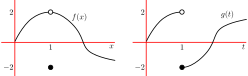
\includegraphics[height=4cm]{lim3}
\end{center}
\end{efig}
These are a little different from our previous examples, in that we do not have
formulas, only the sketch. But we can still compute the limits.
\begin{itemize}
 \item Function on the left --- $f(x)$:
\begin{align*}
  \lim_{x \to 1^-} f(x) &= 2 &
  \lim_{x \to 1^+} f(x) &= 2 \\
\intertext{so by the previous theorem }
\lim_{x \to 1} f(x) &= 2
\end{align*}
 \item Function on the right --- $g(t)$:
\begin{align*}
  \lim_{t \to 1^-} g(t) &= 2
  & \text{and } \lim_{t \to 1^+} g(t) &= -2
\intertext{so by the previous theorem }
  \lim_{t \to 1} g(t) &= \text{DNE}
\end{align*}
\end{itemize}
\end{eg}

We have seen 2 ways in which a limit does not exist --- in one case the
function oscillated wildly, and in the other there was some sort of ``jump'' in
the function, so that the left-hand and right-hand limits were different.

There is a third way that we must also consider. To describe this, consider the
following four functions:
\begin{fig}
\label{fig inf limits}
\begin{center}
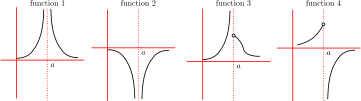
\includegraphics[width = \textwidth]{lim4}
\end{center}
\end{fig}
None of these functions are defined at $x=a$, nor do the limits as $x$
approaches $a$ exist. However we can say more than just ``the limits do not
 exist''.

Notice that the value of function~1 can be made bigger and bigger as we bring
$x$ closer and closer to $a$. Similarly the value of the second function can be
made arbitrarily large and negative (i.e. make it as big a negative number as we
want) by bringing $x$ closer and closer to~$a$. Based on this observation we
have the following definition.
\begin{defn}
\label{def lim is inf informal}
  We write
 \begin{align*}
  \lim_{x \to a} f(x) = + \infty
 \end{align*}
  when the value of the function $f(x)$ becomes arbitrarily large and
  positive as $x$ gets closer and closer to $a$, without being exactly $a$.

  Similarly, we write
 \begin{align*}
  \lim_{x \to a} f(x) = - \infty
 \end{align*}
  when the value of the function $f(x)$ becomes arbitrarily large and
  negative as $x$ gets closer and closer to $a$, without being exactly $a$.
\end{defn}
A good examples of the above is
\begin{align*}
  \lim_{x \to 0} \frac{1}{x^2} &= +\infty
  & \lim_{x \to 0} -\frac{1}{x^2} &= -\infty
\end{align*}
\textbf{IMPORTANT POINT: } Please do not think of ``$+\infty$'' and ``$-\infty$''
in these statements as numbers. You should think of $\lim\limits_{x\rightarrow a} f(x) = +\infty$ and $\lim\limits_{x\rightarrow a} f(x) = -\infty$
as special cases of  $\lim\limits_{x\rightarrow a} f(x) = \text{DNE}$. The statement
\begin{align*}
  \lim_{x \to a} f(x) = +\infty
\end{align*}
does not say ``the limit of $f(x)$ as $x$ approaches $a$ is positive infinity''.
It says ``the function $f(x)$ becomes arbitrarily large as $x$ approaches $a$''.
These are different statements; remember that $\infty$ is not a
number\footnote{One needs to be very careful making statements about
infinity. At some point in our lives we get around to asking ourselves ``what
is the biggest number'', and we realise there isn't one. That is, we can go on
counting integer after integer, for ever and not stop. Indeed the set of
integers is the first infinite thing we really encounter. It is an example of a
\emph{countably infinite} set. The set of real-numbers is actually much bigger
and is \emph{uncountably infinite}. In fact there are an infinite number of
different sorts of infinity! Much of the theory of infinite sets was
developed by Georg Cantor; we mentioned him back in Section~\ref{sec sets} and he is well
worth googling.}.



Now consider functions~3 and~4 in Figure~\ref{fig inf limits}. Here we can make
the value of the function as big and positive as we want (for function~3) or as
big and negative as we want (for function~4) but only when $x$ approaches $a$
from one side. With this in mind we can construct similar notation and a
similar definition:
\begin{defn}
\label{def onesidedlim is inf informal}
  We write
 \begin{align*}
  \lim_{x \to a^+} f(x) = + \infty
 \end{align*}
  when the value of the function $f(x)$ becomes arbitrarily large and
  positive as $x$ gets closer and closer to $a$ from above (equivalently ---
from the right), without being exactly $a$.

  Similarly, we write
 \begin{align*}
  \lim_{x \to a^+} f(x) = - \infty
 \end{align*}
  when the value of the function $f(x)$ becomes arbitrarily large and
  negative as $x$ gets closer and closer to $a$ from above (equivalently ---
from the right), without being exactly $a$.

  The notation
\begin{align*}
  \lim_{x \to a^-} f(x) &= + \infty
&
  \lim_{x \to a^-} f(x) &= - \infty
\end{align*}
  has a  similar meaning except that limits are approached from below / from
the left.
\end{defn}
So for function~3 we have
\begin{align*}
  \lim_{x\to a^-} f(x) &= +\infty
&
  \lim_{x\to a^+} f(x) &= \text{some positive number}
\end{align*}
and for function~4
\begin{align*}
  \lim_{x\to a^-} f(x) &= \text{some positive number}
&
  \lim_{x\to a^+} f(x) &= -\infty
\end{align*}

More examples:
\begin{eg}\label{eg_1_3_5}
Consider the function
\begin{align*}
  g(x) &= \frac{1}{\sin(x)}
\end{align*}
Find the one-sided limits of this function as $x \to \pi$.

Probably the easiest way to do this is to first plot the graph of $\sin(x)$ and
$1/x$ and then think carefully about the one-sided limits:
\begin{efig}
\begin{center}
 \includegraphics[width=0.8\textwidth]{sinx_1onx}
\end{center}
\end{efig}
\begin{itemize}
 \item As $x \to \pi$ from the left, $\sin(x)$ is a small positive number that
is getting closer and closer to zero. That is, as $x \to \pi^-$, we have that
$\sin(x) \to 0$ through positive numbers (i.e. from above). Now look at the graph
of $1/x$, and think what happens as we move $x \to 0^+$, the function is
positive and becomes larger and larger.

So as $x \to \pi$ from the left, $\sin(x) \to 0$ from above, and so $1/\sin(x)
\to +\infty$.

\item By very similar reasoning, as $x \to \pi$ from the right, $\sin(x)$ is a
small negative number that gets closer and closer to zero. So as $x \to \pi$
from the right, $\sin(x) \to 0$ through negative numbers (i.e. from below) and so
$1/\sin(x)$ to $-\infty$.
\end{itemize}
Thus
\begin{align*}
  \lim_{x \to \pi^-} \frac{1}{\sin(x)} &= +\infty &
  \lim_{x \to \pi^+} \frac{1}{\sin(x)} &= -\infty
\end{align*}
\end{eg}


Again, we can make Definitions~\ref{def lim is inf informal}
and~\ref{def onesidedlim is inf informal} into mathematically precise formal
definitions using techniques very similar to those in the optional
Section~\ref{sec opt formal limit}. This is not strictly necessary for this
course.

Up to this point we explored limits by sketching graphs or plugging values into
a calculator. This was done to help build intuition, but it is not really the
basis of a systematic method for computing limits. We have also avoided more
formal approaches\footnote{The formal
approaches are typically referred to as ``epsilon-delta limits'' or
``epsilon-delta proofs'' since the symbols $\epsilon$ and $\delta$ are
traditionally used throughout. Take a peek at Section~\ref{sec opt
formal limit} to see.} since we do not have time in the course to go into
that level of detail and (arguably) we don't need that detail to achieve the
aims of the course. Thankfully we can develop a more systematic approach based
on the idea of building up complicated limits from simpler ones by examining how
limits interact with the basic operations of arithmetic.

\section{Calculating Limits with Limit Laws}\label{sec_1_4}
Think back to the functions you know and the sorts of things you have  been
asked to draw, factor and so on. Then they are all constructed from simple
pieces, such as
\begin{itemize}
 \item constants --- $c$
 \item monomials --- $x^n$
 \item trigonometric functions --- $\sin(x), \cos(x)$ and $\tan(x)$
\end{itemize}
These are the building blocks from which we construct functions. Soon we will
add a few more functions to this list, especially the exponential function and
various inverse functions.

We then take these building blocks and piece them together using arithmetic
\begin{itemize}
 \item addition and subtraction --- $f(x)  = g(x) + h(x)$ and $f(x) = g(x) -
h(x)$
 \item multiplication --- $f(x) = g(x) \cdot h(x)$
 \item division --- $f(x) = \frac{g(x)}{h(x)}$
 \item substitution --- $f(x) = g( h(x) )$ --- this is also called
the composition of $g$ with $h$.
\end{itemize}
The idea of building up complicated functions from simpler pieces was discussed
in Section~\ref{sec parsing}.

What we will learn in this section is how to compute the limits of the basic
building blocks and then how we can compute limits of sums, products and so
forth using ``limit laws''. This process allows us to compute limits of
complicated functions, using very simple tools and without having to resort to
``plugging in numbers'' or ``closer and closer'' or ``$\epsilon-\delta$
arguments''.


In the examples we saw above, almost all the \emph{interesting} limits happened
at points where the underlying function was badly behaved --- where it jumped,
was not defined or blew up to infinity. In those cases we had to be careful and
think about what was happening. Thankfully most functions we will see do not
have too many points at which these sorts of things happen.

For example, polynomials do not have any nasty jumps and are defined everywhere
and do not ``blow up''. If you plot them, they look smooth\footnote{We have
used this term in an imprecise way, but it does have a precise
mathematical meaning.}. Polynomials and limits behave very nicely together,
and for any polynomial $P(x)$ and any real number $a$ we have that
\begin{align*}
  \lim_{x \to a} P(x) &= P(a)
\end{align*}
That is --- to evaluate the limit we just plug in the number. We will build up
to this result over the next few pages.

Let us start with the two easiest limits\footnote{Though it lies outside the
scope of the course, you can find the formal $\epsilon$-$\delta$ proof of this
result at the end of Section~\ref{sec opt formal limit}.}
\begin{theorem}[Easiest limits]\label{thm_easy_lim}
\label{thm easy lim}
   Let $a,c \in \mathbb{R}$. The following two limits hold
  \begin{align*}
  \lim_{x \to a} c & = c & \text{ and }&&
  \lim_{x \to a} x &= a.
\end{align*}
\end{theorem}

Since we have not seen too many theorems yet, let us examine it carefully piece
by piece.
\begin{itemize}
 \item \textbf{Let $a,c \in \mathbb{R}$} --- just as was the case for
definitions, we start a theorem by defining terms and setting the scene. There
is not too much scene to set: the symbols $a$ and $c$ are real numbers.
 \item \textbf{The following two limits hold} --- this doesn't really
contribute much to the statement of the theorem, it just makes it easier to
read.
 \item $\ds \mathbf{\lim_{x \to a} c  = c}$  --- when we take the
limit of a
constant function (for example think of $c=3$), the limit is (unsurprisingly)
just that same constant.
 \item $\ds \mathbf{\lim_{x \to a} x = a}$ --- as we noted above for general
polynomials, the limit of the function $f(x) = x$ as $x$ approaches a given
point $a$, is just $a$. This says something quite obvious --- as $x$ approaches
$a$, $x$ approaches $a$ (if you are not convinced then sketch the graph).
\end{itemize}


Armed with only these two limits, we cannot do very much. But combining these
limits with some arithmetic we can do quite a lot. For a moment, take a step
back from limits for a moment and think about how we construct functions. To
make the discussion a little more precise think about how we might construct
the function
\begin{align*}
  h(x) &= \frac{2x-3}{x^2+5x-6}
\end{align*}

If we want to compute the value of the function at
$x=2$, then we would
\begin{itemize}
 \item compute the numerator at $x=2$
 \item compute the denominator at $x=2$
 \item compute the ratio
\end{itemize}
Now to compute the numerator we
\begin{itemize}
 \item take $x$ and multiply it by 2
 \item subtract 3 to the result
\end{itemize}
While for the denominator
\begin{itemize}
 \item multiply $x$ by $x$
 \item multiply $x$ by 5
 \item add these two numbers and subtract $6$
\end{itemize}
This sequence of operations can be represented pictorially
as the tree shown in Figure~\ref{fig parse me} below.
\begin{fig}
\label{fig parse me}
 \begin{center}
  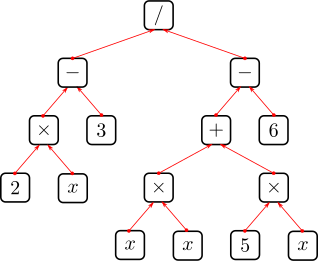
\includegraphics[scale=0.5]{tree3}
 \end{center}
\end{fig}
Such trees were discussed in Section~\ref{sec parsing} (now is not a bad time to quickly
review that section before proceeding). The point here is that in order to compute the
value of the function we just repeatedly add, subtract, multiply and divide constants and
$x$.


To compute the limit of the above function at $x=2$ we can do something very
similar. From the previous theorem we know how to compute
\begin{align*}
  \lim_{x \to 2} c &= c && \text{and} & \lim_{x \to 2} x &= 2
\end{align*}
and the next theorem will tell us how to stitch together these two limits using
the arithmetic we used to construct the function.

\begin{theorem}[Arithmetic of limits]\label{thm arith lim}
  Let $a,c \in \mathbb{R}$, let $f(x)$ and $g(x)$ be defined for all $x$'s that lie in
some interval about $a$ (but $f,g$ need not be defined exactly at $a$).
 \begin{align*}
  \lim_{x \to a} f(x)&=F & \lim_{x \to a} g(x) &=G
\end{align*}
  exist with $F,G \in \mathbb{R}$. Then the following limits hold
\begin{itemize}
 \item $\ds \lim_{x \to a} ( f(x) + g(x) ) = F+G$ --- limit of the sum is the
sum of the limits.
 \item $\ds \lim_{x \to a} ( f(x) - g(x) ) = F - G$ --- limit of the difference
is the difference of the limits.
\item $\ds \lim_{x \to a} c f(x) = c F$.
\item $\ds \lim_{x \to a} ( f(x) \cdot g(x) ) = F \cdot G$ --- limit of
the product is the product of limits.
\item If $G \neq 0$ then $\ds \lim_{x \to a} \frac{f(x)}{g(x)} = \frac{F}{G}$
\end{itemize}
Note --- be careful with this last one --- the denominator cannot be zero.
\end{theorem}
The above theorem shows that limits interact very simply with arithmetic. If
you are asked to find the limit of a sum then the answer is just the sum of the
limits. Similarly the limit of a product is just the product of the limits.


How do we apply the above theorem to the rational function $h(x)$ we defined
above? Here is a warm-up example:
\begin{eg}\label{eg_1_4_1}
You are given two functions $f,g$ (not explicitly) which have the following
limits as $x$ approaches 1:
\begin{align*}
  \lim_{x \to 1} f(x)&=3 && \text{and} & \lim_{x\to 1} g(x)&=2
\end{align*}
Using the above theorem we can compute
\begin{align*}
 \lim_{x \to 1} 3f(x) &= 3 \times 3 = 9 \\
 \lim_{x \to 1} 3f(x) -g(x) &= 3\times 3 -2 = 7\\
 \lim_{x \to 1} f(x) g(x) &= 3\times 2 = 6\\
 \lim_{x \to 1} \frac{f(x)}{f(x) -g(x)} &= \frac{3}{3-2} = 3
\end{align*}
\end{eg}

Another simple example
\begin{eg}\label{eg_1_4_2}
 Find $\ds \lim_{x \to 3} 4x^2-1$

 We use the arithmetic of limits:
\begin{align*}
  \lim_{x \to 3} 4x^2-1
  &= \left( \lim_{x \to 3} 4x^2 \right) - \lim_{x \to 3} 1
  & \text{difference of limits}
\\
  &= \left( \lim_{x \to 3} 4  \cdot \lim_{x \to 3} x^2 \right) -  \lim_{x \to
3} 1
  & \text{product of limits} \\
  &= 4 \cdot \left( \lim_{x \to 3} x^2 \right) -  1
  & \text{limit of constant} \\
  &= 4 \cdot \left( \lim_{x \to 3} x \right) \cdot \left( \lim_{x \to 3} x
\right)-1
  & \text{product of limits} \\
  &= 4 \cdot 3 \cdot 3 - 1
  & \text{limit of $x$} \\
  &= 36 - 1 \\
  &= 35
\end{align*}
\end{eg}
This is an excruciating level of detail, but when you first use this theorem
and try some examples it is a good idea to do things step by step by step until
you are comfortable with it.
\begin{eg}\label{eg_1_4_3}
Yet another limit --- compute $\ds \lim_{x\to 2} \frac{x}{x-1}$.

To apply the arithmetic of limits, we need to examine numerator and
denominator separately and make sure the limit of the denominator is non-zero.
Numerator first:
\begin{align*}
  \lim_{x \to 2} x & = 2 & \text{limit of $x$}
\intertext{and now the denominator:}
  \lim_{x \to 2} x-1
  & = \left( \lim_{x \to 2} x \right) - \left( \lim_{x \to 2} 1 \right)
  & \text{difference of limits} \\
  & = 2 - 1
  & \text{limit of $x$ and limit of constant}
  & = 1
\end{align*}
Since the limit of the denominator is non-zero we can put it back together to
get
\begin{align*}
  \lim_{x\to 2} \frac{x}{x-1} &= \frac{\ds \lim_{x\to 2} x}{\ds \lim_{x \to
2}(x-1)}  \\
  &= \frac{2}{1} \\
  &= 2
\end{align*}
\end{eg}

In the next example we show that many different things can happen if
the limit of the denominator is zero.
\begin{eg}[Be careful with limits of ratios]\label{eg lim rat}
We must be careful when computing the limit of a ratio --- it
is the ratio of the limits except when the limit of the denominator is zero.
When the limit of the denominator is zero Theorem~\ref{thm arith lim}
\textbf{does not apply} and a few interesting things can happen
\begin{itemize}
 \item If the limit of the numerator is non-zero then the limit of the ratio
does not exist
\begin{align*}
  \lim_{x \to a} \frac{f(x)}{g(x)} &= DNE & \text{when $\lim_{x\to a} f(x) \neq
0$ and $\lim_{x \to a} g(x)=0$}
\end{align*}
  For example, $\ds \lim_{x \to 0} \frac{1}{x^2} = DNE$.
 \item If the limit of the numerator is zero then the above theorem does not
give us enough information to decide whether or not the limit exists. It is
possible that
\begin{itemize}
 \item the limit does not exist, eg. $\ds \lim_{x \to 0} \frac{x}{x^2} =
\lim_{x
\to 0} \frac{1}{x} = DNE$
 \item the limit is $\pm \infty$, eg. $\ds \lim_{x \to 0} \frac{x^2}{x^4} =
\lim_{x
\to 0} \frac{1}{x^2} = +\infty$ or $\ds \lim_{x \to 0} \frac{-x^2}{x^4} =
\lim_{x\to 0} \frac{-1}{x^2} = -\infty$.
 \item the limit is zero, eg. $\ds \lim_{x \to 0} \frac{x^2}{x} = 0$
 \item the limit exists and is non-zero, eg. $\ds \lim_{x \to 0} \frac{x}{x} =
1$
\end{itemize}
\end{itemize}
Now while the above examples are very simple and a little contrived they serve
to illustrate the point we are trying to make --- be careful if the limit of
the denominator is zero.
\end{eg}



We now have enough theory to return to our rational function and compute its
limit as $x$ approaches 2.
\begin{eg}\label{eg_1_4_4}
 Let $\ds h(x) = \frac{2x-3}{x^2+5x-6}$ and find its limit as $x$ approaches
$2$.

Since this is the limit  of a ratio, we compute the limit of the numerator and
denominator separately.
Numerator first:
\begin{align*}
  \lim_{x \to 2} 2x-3
  &= \left( \lim_{x \to 2} 2x \right) - \left( \lim_{x \to 2} 3 \right)
  & \text{difference of limits} \\
  &= 2 \cdot \left( \lim_{x \to 2} x \right) -3
  & \text{product of limits and limit of constant} \\
  &= 2 \cdot 2 -3
  & \text{limits of $x$} \\
  &= 1
\end{align*}
Denominator next:
\begin{align*}
  \lim_{x \to 2} x^2+5x-6
  &= \left( \lim_{x \to 2} x^2 \right) + \left( \lim_{x \to 2} 5x \right)
  - \left( \lim_{x \to 2} 6 \right)
  & \text{sum of limits} \\
  &= \left( \lim_{x \to 2} x \right)\cdot \left( \lim_{x \to 2} x \right)
  + 5 \cdot \left( \lim_{x \to 2} x \right) - 6
  & \text{product of limits and limit of constant} \\
  &= 2 \cdot 2 + 5 \cdot 2 - 6
  & \text{limits of $x$} \\
  &= 8
\end{align*}
Since the limit of the denominator is non-zero, we can obtain our result by
taking the ratio of the separate limits.
\begin{align*}
\lim_{x \to 2} \frac{2x-3}{x^2+5x-6}
  &= \frac{\ds \lim_{x \to 2} 2x-3}{\ds \lim_{x \to 2} x^2+5x-6} = \frac{1}{8}
\end{align*}

The above works out quite simply. However, if we were to take the limit as $x
\to 1$ then things are a bit harder. The limit of the numerator is:
\begin{align*}
  \lim_{x \to 1} 2x-3 &= 2 \cdot 1 - 3 = -1
\end{align*}
(we have not listed all the steps). And the limit of the denominator is
\begin{align*}
  \lim_{x \to 1} x^2 +5x-6 &= 1 \cdot 1 + 5 - 6 = 0
\end{align*}
Since the limit of the numerator is non-zero, while the limit of the
denominator is zero, the limit of the ratio does not exist.
\begin{align*}
\lim_{x \to 1} \frac{2x-3}{x^2+5x-6}
  &= DNE
\end{align*}
\end{eg}
It is \textbf{IMPORTANT TO NOTE} that it is not correct to write
\begin{align*}
\lim_{x \to 1} \frac{2x-3}{x^2+5x-6}
  &= \frac{-1}{0} = DNE
\end{align*}
Because we can only write
\begin{align*}
  \lim_{x \to a} \frac{f(x)}{g(x)} &= \frac{\ds \lim_{x \to a} f(x)}{\ds
\lim_{x \to a} g(x) } = \text{something}
\end{align*}
when the limit of the denominator is non-zero (see Example~\ref{eg lim rat} above).

With a little care you can use the arithmetic of limits to obtain the
following rules for limits of powers of functions and limits of roots of
functions:
\begin{theorem}[More arithmetic of limits --- powers and roots]
\label{thm lim powers}
  Let $n$ be a positive integer, let $a \in \mathbb{R}$ and let $f$ be a
function so that
\begin{align*}
  \lim_{x \to a} f(x) &= F
\end{align*}
  for some real number $F$. Then the following holds
\begin{align*}
  \lim_{x \to a} \left( f(x) \right)^n
  &= \left(\lim_{x \to a} f(x) \right)^n = F^n
\end{align*}
so that the limit of a power is the power of the limit. Similarly, if
\begin{itemize}
 \item $n$ is an even number and $F>0$, or
 \item $n$ is an odd number and $F$ is any real number
\end{itemize}
then
\begin{align*}
  \lim_{x \to a} \left( f(x) \right)^{1/n}
  &= \left(\lim_{x \to a} f(x) \right)^{1/n} = F^{1/n}
\end{align*}
More generally\footnote{You may not know the definition of the power
$b^p$ when $p$ is not a rational number, so here it is. If $b>0$ and $p$
is any real number, then $b^p$ is the limit of $b^r$ as $r$ approaches $p$ 
through rational numbers. We won't do so here, but it is possible to prove that the limit exists.}, if $F>0$ and $p$ is any real number,
\begin{align*}
  \lim_{x \to a} \left( f(x) \right)^p
  &= \left(\lim_{x \to a} f(x) \right)^p = F^p
\end{align*}
\end{theorem}
Notice that we have to be careful when taking roots of limits that might be
negative numbers. To see why, consider the case $n=2$, the limit
\begin{align*}
  \lim_{x \to 4} x^{1/2} &= 4^{1/2} = 2 \\
  \lim_{x \to 4} (-x)^{1/2} &= (-4)^{1/2} = \text{not a real number}
\end{align*}
In order to evaluate such limits properly we need to use complex numbers which
are beyond the scope of this text.

Also note that the notation $x^{1/2}$ refers to the \emph{positive} square root
of $x$. While $2$ and $(-2)$ are both square-roots of $4$, the notation
$4^{1/2}$ means $2$. This is something we must be careful of\footnote{Like
ending sentences in prepositions --- ``This is something up with which we will
not put.'' This quote is attributed to Churchill though there is some dispute as to
whether or not he really said it.}.

So again --- let us do a few examples and carefully note what we are doing.
\begin{eg}\label{eg_1_4_5}
\begin{align*}
  \lim_{x \to 2} (4x^2-3)^{1/3} &=
  \left( (\lim_{x\to 2} 4x^2) - (\lim_{x \to 2} 3) \right)^{1/3} \\
  &= \left( 4 \cdot 2^2  - 3 \right)^{1/3}\\
  &= \left( 16-3 \right)^{1/3} \\
  &= 13^{1/3}
\end{align*}
\end{eg}

By combining the last few theorems we can make the evaluation of limits of
polynomials and rational functions much easier:
\begin{theorem}[Limits of polynomials and rational functions]\label{thm_1_4_1}
Let $a \in \mathbb{R}$, let $P(x)$ be a polynomial and let $R(x)$ be a rational
function. Then
\begin{align*}
  \lim_{x \to a} P(x) &= P(a)
\end{align*}
and provided $R(x)$ is defined at $x=a$ then
\begin{align*}
  \lim_{x \to a} R(x) &= R(a)
\end{align*}
If $R(x)$ is not defined at $x=a$ then we are not able to apply this result.
\end{theorem}
So the previous examples are now much easier to compute:
\begin{align*}
\begin{array}{rcccr}
  \ds\lim_{x \to 2} \frac{2x-3}{x^2+5x-6} &=& \ds \frac{4-3}{4+10-6} &=&
\ds \frac{1}{8}\\[3ex]
  \ds\lim_{x\to 2} (4x^2-1) &=& 16-1 &=& 15 \\[1ex]
  \ds\lim_{x\to 2} \frac{x}{x-1} &=& \ds \frac{2}{2-1} &=& 2
\end{array}
\end{align*}


It is clear that limits of polynomials are very easy, while those of rational
functions are easy except when the denominator might go to zero. We have seen
examples where the resulting limit does not exist, and some where it does. We
now work to explain this more systematically. The following example demonstrates that it
is sometimes possible to take the limit of a rational function to a point at which the
denominator is zero. Indeed we must be able to do exactly this in order to be able to
define derivatives in
the next chapter.
\begin{eg}\label{eg zero cancel limit}
Consider the limit
\begin{align*}
    \lim_{x \to 1} \frac{x^3-x^2}{x-1}.
\end{align*}
If we try to apply the arithmetic of limits then we compute the limits of the
numerator and denominator separately
\begin{align}
    \lim_{x \to 1} x^3-x^2 &= 1-1 = 0 \\
    \lim_{x \to 1} x-1 &= 1-1 = 0
\end{align}
Since the denominator is zero, we cannot apply our theorem and we are, for the
moment, stuck. However, there is more that we can do here --- the hint is that
the numerator and denominator \emph{both} approach zero as $x$ approaches 1. This
means that there might be something we can cancel.

So let us play with the expression a little more before we take the limit:
\begin{align*}
  \frac{x^3-x^2}{x-1} &= \frac{x^2(x-1)}{x-1} = x^2
  & \text{ provided $x \neq 1$.}
\end{align*}
So what we really have here is the following function
\begin{align*}
  \frac{x^3-x^2}{x-1} &= \begin{cases}
                          x^2 & x \neq 1 \\
                          \text{undefined } & x = 1
                         \end{cases}
\end{align*}
If we plot the above function the graph looks exactly the same as $y=x^2$
except that the function is not defined at $x=1$ (since at $x=1$ both numerator and
denominator are zero).
\begin{efig}
\begin{center}
 \includegraphics[height=4cm]{rat1}
\end{center}
\end{efig}
When we compute a limit as $x \to a$, the value of the function exactly at
$x=a$ is irrelevant. We only care what happens to the function as we bring $x$
very close to $a$. So for the above problem we can write
\begin{align*}
    \frac{x^3-x^2}{x-1} &= x^2 & \text{when $x$ is close to $1$ but not at
$x=1$}
\end{align*}
So the limit as $x \to 1$ of the function is the same as the limit $\ds \lim_{x\to
1} x^2$ since the functions are the same except exactly at $x=1$. By this
reasoning we get
\begin{align*}
    \lim_{x \to 1} \frac{x^3-x^2}{x-1} &=
    \lim_{x \to 1} x^2 = 1
\end{align*}
\end{eg}
The reasoning in the above example can be made more general:
\begin{theorem}\label{thm_1_4_2}
 If $f(x) = g(x)$ except when $x=a$ then $\ds \lim_{x\to a} f(x) = \lim_{x\to
a}
g(x)$ provided the limit of $g$ exists.
\end{theorem}

How do we know when to use this theorem? The big clue is that when we try to
compute the limit in a naive way, we end up with $\frac{0}{0}$. We know that
$\frac{0}{0}$ does not make sense, but it is an indication that there might be a
common factor between numerator and denominator that can be cancelled. In the
previous example, this common factor was $(x-1)$.

\begin{eg}\label{eg easy 0on0 limit}
  Using this idea compute
 \begin{align*}
  \lim_{h \to 0} \frac{(1+h)^2-1}{h}
 \end{align*}

\begin{itemize}
 \item First we should check that we cannot just substitute $h=0$ into this ---
clearly we cannot because the denominator would be $0$.
\item But we should also check the numerator to see if we have $\frac{0}{0}$, and we see
that the numerator gives us $1-1 = 0$.
\item Thus we have a hint that there is a common factor that we might be able to
cancel. So now we look for the common factor and try to cancel it.
\begin{align*}
  \frac{(1+h)^2-1}{h} &= \frac{1+2h+h^2-1}{h} & \text{expand} \\
  &= \frac{2h+h^2}{h} = \frac{h(2+h)}{h} & \text{factor and then cancel}\\
  &= 2+h
\end{align*}
\item Thus we really have that
\begin{align*}
  \frac{(1+h)^2-1}{h}&= \begin{cases}
                         2+h & h \neq 0\\
			\text{undefined} & h=0
                        \end{cases}
\end{align*}
and because of this
\begin{align*}
  \lim_{h \to 0} \frac{(1+h)^2-1}{h}
  &= \lim_{h \to 0} 2+h \\
  &= 2
\end{align*}
\end{itemize}
\end{eg}
Of course --- we have written everything out in great detail here and
that is way more than is required for a solution to such a problem. Let us do
it again a little more succinctly.
\begin{eg}\label{eg_1_4_6}
 Compute the following limit:
 \begin{align*}
  \lim_{h \to 0} \frac{(1+h)^2-1}{h}
 \end{align*}
  If we try to use the arithmetic of limits, then we see that the limit of the
numerator and the limit of the denominator are both zero. Hence we should try
to factor them and cancel any common factor. This gives
 \begin{align*}
  \lim_{h \to 0} \frac{(1+h)^2-1}{h}
  &= \lim_{h \to 0} \frac{1+2h+h^2-1}{h} \\
  &= \lim_{h \to 0} 2+h \\
  &= 2
 \end{align*}
\end{eg}
Notice that even though we did this example carefully above, we have still
written some text in our working explaining what we have done. You should
always think about the reader and if in doubt, put in more explanation rather
than less. We could make the above example even more terse
\begin{eg}\label{eg_1_4_7}
 Compute the following limit:
 \begin{align*}
  \lim_{h \to 0} \frac{(1+h)^2-1}{h}
 \end{align*}
 Numerator and denominator both go to zero as $h\to 0$. So factor and simplify:
 \begin{align*}
  \lim_{h \to 0} \frac{(1+h)^2-1}{h}
  &= \lim_{h \to 0} \frac{1+2h+h^2-1}{h} \\
  &= \lim_{h \to 0} 2+h = 2
 \end{align*}
\end{eg}


A slightly harder one now
\begin{eg}\label{eg zero cancel limit harder}
Compute the limit
  \begin{align*}
  \lim_{x \to 0} \frac{x}{\sqrt{1+x}-1}
  \end{align*}
If we try to use the arithmetic of limits we get
\begin{align*}
  \lim_{x \to 0} x &= 0 \\
  \lim_{x \to 0} \sqrt{1+x}-1 &= \sqrt{ \lim_{x \to 0} 1+x}-1 = 1-1 =0
\end{align*}
So doing the naive thing we'd get $0/0$. This suggests a common factor that can
be cancelled. Since the numerator and denominator are not polynomials we have
to try other tricks%
%%%
\footnote{While these tricks are useful (and even cute\protect\footnotemark),
Taylor polynomials (see Section~\ref{sec:DIFFTaylor}) give us a more systematic
way of approaching this problem.}%
\footnotetext{Mathematicians tend to have quite strong opinions on the
beauty of mathematics. For example, Paul Erd\"os\protect\footnotemark
said ``Why are numbers beautiful? It's like asking why is Beethoven's Ninth
Symphony beautiful. If you don't see why, someone can't tell you. I know
numbers are beautiful. If they aren't beautiful, nothing is.''.}%
\footnotetext{Arguably the most prolific mathematician of the 20th century
--- definitely worth a google. The authors do not know his opinion on nested
footnotes\protect\footnotemark.}%
\footnotetext{Nested footnotes are generally frowned upon, since they can get
quite contorted; see XKCD-1208 and also the novel ``House of Leaves'' by Mark Z.
Danielewski.}
%%%%
. We can simplify the denominator $\sqrt{1+x}-1$ a
lot, and in particular eliminate the square root, by multiplying it by
its conjugate $\sqrt{1+x}+1$.
\begin{align*}
  \frac{x}{\sqrt{1+x}-1}
  &=\frac{x}{\sqrt{1+x}-1} \times \frac{\sqrt{1+x}+1}{\sqrt{1+x}+1}
  & \text{multiply by $\frac{\text{conjugate}}{\text{conjugate}}=1$} \\
    &=\frac{x \left( \sqrt{1+x}+1\right)}
  {\left(\sqrt{1+x}-1\right)\left(\sqrt{1+x}+1\right)}
  & \text{bring things together } \\
    &=\frac{x \left( \sqrt{1+x}+1\right)}
  {\left(\sqrt{1+x}\right)^2 - 1\cdot 1}
  & \text{since $(a-b)(a+b)=a^2-b^2$} \\
    &=\frac{x \left( \sqrt{1+x}+1\right)}
  {1+x - 1}
  & \text{clean up a little} \\
    &=\frac{x \left( \sqrt{1+x}+1\right)}{x} \\
  &= \sqrt{1+x}+1
  & \text{cancel the $x$} \\
\end{align*}
So now we have
  \begin{align*}
  \lim_{x \to 0} \frac{x}{\sqrt{1+x}-1}
  &= \lim_{x \to 0} \sqrt{1+x}+1 \\
  &= \sqrt{1+0}+1 = 2
  \end{align*}
\end{eg}
How did we know what to multiply by? Our function was of the form
\begin{align*}
  \frac{a}{\sqrt{b} - c}
\end{align*}
so, to eliminate the square root from the denominator, we employ a trick --- we multiply
by 1. Of course, multiplying by 1 doesn't do anything. But if you multiply by 1
carefully you can leave the value the same, but change the form of the
expression. More precisely
\begin{align*}
  \frac{a}{\sqrt{b} - c}
  &= \frac{a}{\sqrt{b} - c} \cdot 1 \\
  &= \frac{a}{\sqrt{b} - c} \cdot
\underbrace{\frac{\sqrt{b}+c}{\sqrt{b}+c}}_{=1} \\
  &= \frac{a \left(\sqrt{b}+c \right)}
  {\left(\sqrt{b} - c\right)\left(\sqrt{b}+c \right)}
  & \text{expand denominator carefully} \\
  &= \frac{a \left(\sqrt{b}+c \right)}
  {\sqrt{b} \cdot \sqrt{b} - c\sqrt{b} + c\sqrt{b} - c\cdot c}
  & \text{do some cancellation} \\
  &= \frac{a \left(\sqrt{b}+c \right)} {b - c^2}
\end{align*}
Now the numerator contains roots, but the denominator is just a polynomial.


Before we move on to limits at infinity, there is one more theorem to see.
While the scope of its application is quite limited, it can be extremely
useful. It is called a sandwich theorem or a squeeze theorem for reasons that
will become apparent.

Sometimes one is presented with an unpleasant ugly function such as
\begin{align*}
  f(x) &= x^2 \sin(\pi/x)
\end{align*}
It is a fact of life, that not all the functions that are encountered in
mathematics will be elegant and simple; this is especially true when the
mathematics gets applied to real world problems. One just has to work with what one gets.
So how can we compute
\begin{align*}
  \lim_{x \to 0} x^2 \sin(\pi/x) ?
\end{align*}
Since it is the product of two functions, we might try
\begin{align*}
  \lim_{x \to 0} x^2 \sin(\pi/x)
  &=
  \left( \lim_{x \to 0} x^2 \right) \cdot \left( \lim_{x \to 0} \sin(\pi/x)
\right)\\
  &= 0 \cdot \left( \lim_{x \to 0} \sin(\pi/x)  \right)\\
  & = 0
\end{align*}
But we just cheated --- we cannot use the arithmetic of limits theorem here, because the
limit
\begin{align*}
  \lim_{x \to 0} \sin(\pi/x) &= DNE
\end{align*}
does not exist. Now we did see the function $\sin(\pi/x)$ before (in
Example~\ref{eg sinpix}), so you should go back and look at it again.
Unfortunately the theorem ``the limit of a product is the product of the
limits'' only holds when the limits you are trying to multiply together actually
exist. So we cannot use it.

However, we do see that the function naturally decomposes into the product of
two pieces --- the functions $x^2$ and $\sin(\pi/x)$. We have sketched the two
functions  in the figure on the left below.
\begin{fig}
\begin{center}
 \includegraphics[width=\textwidth]{squeeze1}\\
\end{center}
\end{fig}
While $x^2$ is a very well behaved function and we know quite a lot about it,
the function $\sin(\pi/x)$ is quite ugly. One of the few things we can say
about it is the following
\begin{align*}
  -1 \leq \sin(\pi/x) \leq 1 && \text{provided $x \neq 0$}
\end{align*}
But if we multiply this expression by $x^2$ we get (because $x^2 \geq 0$)
\begin{align*}
  -x^2 \leq x^2\sin(\pi/x) \leq x^2 && \text{provided $x \neq 0$}
\end{align*}
and we have sketched the result in the figure above (on the right). So the
function we are interested in is \emph{squeezed} or \emph{sandwiched} between
the functions $x^2$ and $-x^2$.

If we focus in on the picture close to $x=0$ we see that $x$ approaches $0$,
the functions $x^2$ and $-x^2$ both approach $0$. Further, because
$x^2\sin(\pi/x)$ is sandwiched between them, it seems that it also approaches
$0$.

The following theorem tells us that this is indeed the case:
\begin{theorem}[Squeeze theorem (or sandwich theorem or pinch theorem)]
\label{thm squeeze}
  Let $a \in \mathbb{R}$ and let $f,g,h$ be three functions so that
  \begin{align*}
    f(x) \leq g(x) \leq h(x)
  \end{align*}
  for all $x$ in an interval around $a$, except possibly exactly at $x=a$. Then
if
  \begin{align*}
    \lim_{x \to a} f(x) &= \lim_{x \to a} h(x) = L
  \end{align*}
  then it is also the case that
  \begin{align*}
    \lim_{x \to a} g(x) &= L
  \end{align*}
\end{theorem}

Using the above theorem we can compute the limit we want and write it up nicely
\begin{eg}\label{eg_1_4_8}
  Compute the limit
\begin{align*}
  \lim_{x \to 0} x^2 \sin(\pi/x)
\end{align*}

  Since $-1 \leq \sin(\theta) \leq 1$ for all real numbers $\theta$, we have
\begin{align*}
  -1 \leq \sin(\pi /x ) \leq 1 && \text{for all $x \neq 0$}
\end{align*}
  Multiplying the above by $x^2$ we see that
\begin{align*}
  -x^2 \leq x^2 \sin(\pi /x ) \leq x^2 && \text{for all $x \neq 0$}
\end{align*}
  Since $\ds \lim_{x \to 0} x^2 = \lim_{x \to 0} (-x^2) = 0$ by the sandwich
(or squeeze or pinch) theorem we have
\begin{align*}
  \lim_{x \to 0} x^2 \sin(\pi/x) &= 0
\end{align*}
\end{eg}
Notice how we have used ``words''. We have remarked on this several times
already in the text, but we will keep mentioning it. It is okay to use words in
your answers to maths problems --- and you should do so! These let the reader
know what you are  doing and help you understand what you are doing.

Another sandwich theorem example
\begin{eg}\label{eg_1_4_9}
Let $f(x)$ be a function such that $1 \leq f(x) \leq x^2-2x+2$. What is
$\ds \lim_{x \to 1} f(x)$?

We are already supplied with an inequality, so it is likely that it is going to
help us. We should examine the limits of each side to see if they are the same:
\begin{align*}
  \lim_{x \to 1} 1 &= 1 \\
  \lim_{x \to 1} x^2-2x+2 &= 1-2+2 = 1
\end{align*}
So we see that the function $f(x)$ is trapped between two functions that both
approach $1$ as $x \to 1$. Hence by the sandwich / pinch / squeeze theorem, we
know that
\begin{align*}
  \lim_{x \to 1} f(x) & =1
\end{align*}
\end{eg}


To get some intuition as to why the squeeze theorem is true, consider when $x$ is very very close to $a$.
In particular, consider when $x$ is sufficiently close to $a$ that we know $h(x)$ is within $10^{-6}$ of $L$
and that $f(x)$ is also within $10^{-6}$ of $L$. That is
\begin{align*}
|h(x)-L| &<10^{-6}  & \text{and}&& |f(x)-L| &<10^{-6}.
\end{align*}
This means that
\begin{align*}
L-10^{-6} &< f(x) \leq h(x) < L+10^{-6}
\end{align*}
since we know that $f(x) \leq h(x)$.

But now by the hypothesis of the squeeze theorem we know that $f(x) \leq g(x) \leq h(x)$ and so we have
\begin{align*}
L-10^{-6} &< f(x) \leq g(x) \leq h(x) < L+10^{-6}
\end{align*}
And thus we know that
\begin{align}
L-10^{-6} &\leq g(x) \leq L+10^{-6}
\end{align}
That is $g(x)$ is also within $10^{-6}$ of $L$.

In this argument our choice of $10^{-6}$ was arbitrary, so we can really replace $10^{-6}$ with any small number we like.
Hence we know that we can force $g(x)$ as close to $L$ as we like, by bringing $x$ sufficiently close to $a$. We give
a more formal and rigorous version of this argument at the end of Section~\ref{sec proof arith lim}.

\section{Limits at Infinity}\label{sec_1_5}
Up until this point we have discussed what happens to a function as we move its input $x$
closer and closer to a particular point $a$. For a great many applications of
limits we need to understand what happens to a function when its input becomes
extremely large --- for example what happens to a population at a time far in
the future.

The definition of a limit at infinity has a similar flavour to the definition of limits at
finite points that we saw above, but the details are a little different. We also
need to distinguish between positive and negative infinity. As $x$ becomes
very large and positive it moves off towards $+\infty$ but when it becomes very
large and negative it moves off towards $-\infty$.


Again we give an informal definition; the full formal definition can be found
in (the optional) Section~\ref{sec lim inf formal} near the end of this chapter.
\begin{defn}[Limits at infinity --- informal]\label{def_1_5_1}
We write
\begin{align*}
\lim_{x \to \infty} f(x) &= L
\end{align*}
when the value of the function $f(x)$ gets closer and closer to $L$ as we make
$x$ larger and larger and positive.

Similarly we write
\begin{align*}
\lim_{x \to -\infty} f(x) &= L
\end{align*}
when the value of the function $f(x)$ gets closer and closer to $L$ as we make
$x$ larger and larger and negative.

\end{defn}

\begin{eg}\label{eg_1_5_1}
Consider the two functions depicted below
\begin{efig}
\begin{center}
 \includegraphics[height=4cm]{lim7}
\end{center}
\end{efig}
The dotted horizontal lines indicate the behaviour as $x$ becomes very large.
The function on the left has limits as $x \to \infty$ and as $x \to -\infty$
since  the function ``settles down'' to a particular value. On the other hand,
the function  on the right does not have a limit as $x \to -\infty$ since the
function just keeps getting bigger and bigger.
\end{eg}

Just as was the case for limits as $x \to a$ we will start with two very simple
building blocks and build other limits from those.
\begin{theorem}
\label{thm basic lim inf}
 Let $c \in \mathbb{R}$ then the following limits hold
\begin{align*}
  \lim_{x \to \infty} c &= c & \lim_{x \to -\infty} c &= c \\
  \lim_{x \to \infty} \frac{1}{x} &= 0 & \lim_{x \to -\infty} \frac{1}{x} &= 0
\end{align*}
\end{theorem}
Again, these limits interact nicely with standard arithmetic:
\begin{theorem}[Arithmetic of limits at infinity]\label{thm_1_5_1}
Let $f(x), g(x)$ be two functions for which the limits
 \begin{align*}
  \lim_{x \to \infty} f(x)&=F & \lim_{x \to \infty} g(x) &=G
\end{align*}
  exist. Then the following limits hold
\begin{align*}
  \lim_{x \to \infty} f(x) \pm g(x) &= F \pm G \\
  \lim_{x \to \infty} f(x) g(x) &= F  G \\
  \lim_{x \to \infty} \frac{f(x)}{ g(x) } &= \frac{F}{G} & \text{provided $G
\neq 0$}
\intertext{and for real numbers $p$}
  \lim_{x \to \infty} f(x)^p &= F^p & \text{provided $F^p$ and $f(x)^p$ are defined for all $x$}
\end{align*}
The analogous results hold for limits to $-\infty$.
\end{theorem}
Note that, as was the case in Theorem~\ref{thm lim powers}, we need a little extra care
with powers of functions. We must avoid taking square roots of negative numbers, or
indeed any even root of a negative number\footnote{To be more precise, there is no real
number $x$ so that $x^\text{even power}$ is a negative number. Hence we cannot take the
even-root of a negative number and express it as a real number. This is precisely
what complex numbers allow us to do, but alas there is not space in the course for us to
explore them.}.



Hence we have for all rational $r>0$
\begin{align*}
  \lim_{x \to \infty} \frac{1}{x^r} &= 0
\end{align*}
but we have to be careful with
\begin{align*}
  \lim_{x \to -\infty} \frac{1}{x^r} &= 0
\end{align*}
This is only true if the denominator of $r$ is not an even
number\footnote{where we write $r = \frac{p}{q}$ with $p,q$ integers with no
common factors. For example,  $r = \frac{6}{14}$ should be written as $r =
\frac{3}{7}$ when considering this rule.}.

For example
\begin{itemize}
 \item $\ds \lim_{x \to \infty} \frac{1}{x^{1/2}} = 0$, but $\ds \lim_{x \to
-\infty} \frac{1}{x^{1/2}}$ does not exist, because $x^{1/2}$ is not defined for
$x<0$.
\item On the other hand, $x^{4/3}$ is defined for negative values of $x$
and $\ds \lim_{x \to -\infty} \frac{1}{x^{4/3}} = 0$.
\end{itemize}

Our first application of limits at infinity will be to examine the behaviour of
a rational function for very large $x$. To do this we use a ``trick''.
\begin{eg}\label{eg_1_5_2}
Compute the following limit:
\begin{align*}
\lim_{x \to \infty} \frac{x^2-3x+4}{3x^2+8x+1}
\end{align*}
As $x$ becomes very  large, it is the $x^2$ term that will dominate in both the
numerator and denominator and the other bits become irrelevant. That is,
for very large $x$, $x^2$ is much much larger than $x$ or any constant. So we
pull out these dominant parts
\begin{align*}
  \frac{x^2-3x+4}{3x^2+8x+1}
  &= \frac{x^2 \left(1-\frac{3}{x}+\frac{4}{x^2}\right)}
  {x^2 \left(3+\frac{8}{x}+\frac{1}{x^2} \right)}\\
  &= \frac{1-\frac{3}{x}+\frac{4}{x^2}}
  {3+\frac{8}{x}+\frac{1}{x^2}} & \text{ remove the common factors}
\end{align*}
\begin{align*}
  \lim_{x \to \infty} \frac{x^2-3x+4}{3x^2+8x+1}
  &= \lim_{x \to \infty} \frac{1-\frac{3}{x}+\frac{4}{x^2}}
  {3+\frac{8}{x}+\frac{1}{x^2}}\\
  &= \frac{\ds \lim_{x \to \infty}\left(1-\frac{3}{x}+\frac{4}{x^2}\right)}
{\ds \lim_{x \to \infty}\left(3+\frac{8}{x}+\frac{1}{x^2} \right)}
& \text{arithmetic of limits} \\
  &= \frac{\ds \lim_{x \to \infty} 1
  - \lim_{x \to \infty} \frac{3}{x} + \lim_{x \to \infty} \frac{4}{x^2}}
{\ds \lim_{x \to \infty} 3
 + \lim_{x \to \infty} \frac{8}{x}+ \lim_{x \to \infty} \frac{1}{x^2} }
& \text{more arithmetic of limits} \\
  &= \frac{1+0+0}{3+0+0}  = \frac{1}{3}
\end{align*}
\end{eg}

The following one gets a little harder
\begin{eg}\label{eg lim tricky}
 Find the limit as $x \to \infty$ of $\frac{\sqrt{4x^2+1}}{5x-1}$

We use the same trick --- try to work out what is the biggest term in the
numerator and denominator and pull it to one side.
\begin{itemize}
 \item The denominator is dominated by $5x$.
 \item The biggest contribution to the numerator comes from the $4x^2$ inside
the square-root. When we pull $x^2$ outside the square-root it becomes $x$,
so the numerator is dominated by $x \cdot \sqrt{4} = 2x$
 \item To see this more explicitly rewrite the numerator
\begin{align*}
  \sqrt{4x^2+1} &= \sqrt{x^2 (4+1/x^2)} = \sqrt{x^2} \sqrt{4+1/x^2} =
x\sqrt{4+1/x^2}.
\end{align*}
\item Thus the limit as $x \to \infty$ is
\begin{align*}
 \lim_{x \to \infty} \frac{\sqrt{4x^2+1}}{5x-1}
 &= \lim_{x \to \infty} \frac{x \sqrt{4+1/x^2}}{x(5-1/x)}\\
 &= \lim_{x \to \infty} \frac{\sqrt{4+1/x^2}}{5-1/x} \\
 & = \frac{2}{5}
\end{align*}
\end{itemize}
\end{eg}

Now let us also think about the limit of the same function,
$\frac{\sqrt{4x^2+1}}{5x-1}$, as $x \rightarrow -\infty$. There is something
subtle going on because of the square-root. First consider the
function\footnote{Just to change things up lets use $t$ and $h(t)$ instead of
the ubiquitous $x$ and $f(x)$.}
\begin{align*}
  h(t) &= \sqrt{t^2}
\end{align*}
Evaluating this at $t=7$ gives
\begin{align*}
  h(7) &= \sqrt{ 7^2 } = \sqrt{49} = 7
\end{align*}
We'll get much the same thing for any $t \geq 0$. For any $t \ge 0$, $h(t)=\sqrt{t^2}$
returns exactly $t$. However now consider the function at $t=-3$
\begin{align*}
  h(-3) &= \sqrt{ (-3)^2 } = \sqrt{9} = 3 = - (-3)
\end{align*}
that is the function is returning $-1$ times the input.

This is because when we defined $\sqrt{\text{ }}$, we defined it to be the
\emph{positive} square-root. i.e. the function $\sqrt{t}$ can never return a
negative number. So being more careful
\begin{align*}
  h(t) &= \sqrt{t^2} = | t |
\end{align*}
Where the $|t|$ is the absolute value of $t$. You are perhaps used to thinking
of absolute value as ``remove the minus sign'', but this is not quite correct.
Let's sketch the function
\begin{fig}
\begin{center}
\includegraphics[height=3cm]{abs}
\end{center}
\end{fig}
It is a piecewise function defined by
\begin{align*}
  |x| &= \begin{cases}
          x & x \geq 0\\
	  -x & x < 0
         \end{cases}
\end{align*}
Hence our function $h(t)$ is really
\begin{align*}
  h(t) &= \sqrt{t^2} =
	  \begin{cases}
          t & t \geq 0\\
	  -t & t < 0
         \end{cases}
\end{align*}
So that when we evaluate $h(-7)$ it is
\begin{align*}
  h(-7) &= \sqrt{ (-7)^2 } = \sqrt{49} = 7 = -(-7)
\end{align*}
We are now ready to examine the limit as $x \to -\infty$ in our previous
example. Mostly it is copy and paste from above.
\begin{eg}\label{eg lim tricky part2}
 Find the limit as $x \to -\infty$ of $\frac{\sqrt{4x^2+1}}{5x-1}$

We use the same trick --- try to work out what is the biggest term in the
numerator and denominator and pull it to one side. Since we are taking the
limit as $x \to -\infty$ we should think of $x$ as a large negative number.
\begin{itemize}
 \item The denominator is dominated by $5x$.
 \item The biggest contribution to the numerator comes from the $4x^2$ inside
the square-root. When we pull the $x^2$ outside a square-root it becomes $|x| =
-x$ (since we are taking the limit as $x \to -\infty$), so the numerator is
dominated by $-x\cdot\sqrt{4} = -2x$
 \item To see this more explicitly rewrite the numerator
\begin{align*}
  \sqrt{4x^2+1} &= \sqrt{x^2 (4+1/x^2)}  = \sqrt{x^2} \sqrt{4+1/x^2} \\
  &= |x|\sqrt{4+1/x^2} & \text{ and since $x<0$ we have} \\
  & = -x\sqrt{4+1/x^2}
\end{align*}
\item Thus the limit as $x \to -\infty$ is
\begin{align*}
 \lim_{x \to -\infty} \frac{\sqrt{4x^2+1}}{5x-1}
 &= \lim_{x \to -\infty} \frac{-x \sqrt{4+1/x^2}}{x(5-1/x)}\\
 &= \lim_{x \to -\infty} \frac{-\sqrt{4+1/x^2}}{5-1/x} \\
 & = -\frac{2}{5}
\end{align*}
\end{itemize}
\end{eg}
So the limit as $x \to -\infty$ is almost the same but we gain a minus sign.
This \textbf{is definitely not} the case in general --- you have to think about each
example separately.

Here is a sketch of the function in question.
\begin{fig}
\begin{center}
 \includegraphics[height=4cm]{neg_inf_lim}
\end{center}
\end{fig}


\begin{eg}\label{eg_1_5_3}
Compute the following limit:
\begin{align*}
  \lim_{x \to \infty} \left( x^{7/5}-x \right)
\end{align*}
In this case we cannot use the arithmetic of limits to write this as
\begin{align*}
  \lim_{x \to \infty} \left( x^{7/5}-x \right)
  &= \left( \lim_{x \to \infty} x^{7/5}\right)
  - \left( \lim_{x \to \infty} x \right) \\
  &= \infty -\infty
\end{align*}
because the limits do not exist. We can only use the limit laws when the limits
exist. So we should go back and think some more.

When $x$ is very large, $x^{7/5} = x\cdot x^{2/5}$ will be much larger than $x$, so the
$x^{7/5}$ term will dominate the $x$ term. So factor out $x^{7/5}$ and rewrite it as
\begin{align*}
  x^{7/5}-x &= x^{7/5} \left(1 - \frac{1}{x^{2/5}} \right)
\end{align*}
Consider what happens to each of the factors as $x \to \infty$
\begin{itemize}
 \item For large $x$, $x^{7/5}>x$ (this is actually true for any $x>1$).
In the limit as $x \to +\infty$, $x$ becomes arbitrarily large and
positive, and $x^{7/5}$ must be bigger still, so it follows that
\begin{align*}
  \lim_{x \to \infty} x^{7/5} &= + \infty.
\end{align*}
 \item On the other hand, $(1-x^{-2/5})$ becomes closer and closer to $1$ ---
we can use the arithmetic of limits to write this as
\begin{align*}
  \lim_{x \to \infty} (1-x^{-2/5}) &= \lim_{x \to \infty} 1 - \lim_{x \to
\infty} x^{-2/5} = 1-0 = 1
\end{align*}
\end{itemize}
So the product of these two factors will be come larger and larger (and
positive) as $x$ moves off to infinity. Hence we have
\begin{align*}
  \lim_{x \to \infty} x^{7/5} \left(1 - 1/x^{2/5} \right) &= + \infty
\end{align*}
\end{eg}
But remember $+\infty$ and $-\infty$ are not numbers; the last equation in the example is
shorthand for ``the function becomes arbitrarily large''.

In the previous section we saw that finite limits and arithmetic interact very nicely
(see Theorems~\ref{thm arith lim} and~\ref{thm lim powers}). This enabled us to compute
the limits of more complicated function in terms of simpler ones. When limits of
functions go to plus or minus infinity we are quite a bit more restricted in what we can
deduce. The next theorem states some results concerning the sum, difference, ratio and
product of infinite limits --- unfortunately in many cases we cannot make general
statements and the results will depend on the details of the problem at hand.

\begin{theorem}[Arithmetic of infinite limits]
\label{thm arith inf lim}
 Let $a,c,H \in \mathbb{R}$ and let $f,g,h$ be functions defined in
an interval around $a$ (but they need not be defined at $x=a$), so that
\begin{align*}
  \lim_{x \to a} f(x) &= +\infty &
  \lim_{x \to a} g(x) &= +\infty &
  \lim_{x \to a} h(x) &= H
\end{align*}
\begin{itemize}
 \item $\ds \lim_{x \to a} ( f(x) + g(x) ) = +\infty$
 \item $\ds \lim_{x \to a} ( f(x) + h(x) ) = +\infty$
 \item $\ds \lim_{x \to a} ( f(x) - g(x) )$ undetermined
 \item $\ds \lim_{x \to a} ( f(x) - h(x) ) = +\infty$
 \item $\ds \lim_{x \to a} c f(x) =
\begin{cases}
 +\infty & c>0 \\
0 & c=0 \\
-\infty & c<0
\end{cases}
$
\item $\ds \lim_{x \to a} ( f(x) \cdot g(x) ) = +\infty$.
\item $\ds \lim_{x \to a} f(x) h(x) =
\begin{cases}
 +\infty & H>0 \\
-\infty & H<0\\
\text{undetermined} & H=0
\end{cases}
$
\item $\ds \lim_{x \to a} \frac{f(x)}{g(x)}$ undetermined
\item $\ds \lim_{x \to a} \frac{f(x)}{h(x)} =
\begin{cases}
+\infty & H>0 \\
-\infty & H<0\\
\text{undetermined} & H=0
\end{cases}$

%\end{itemize}
%\end{theorem}
%
%\addtocounter{theorem}{-1}
%\begin{theorem}[continued]
%\begin{itemize}

\item $\ds \lim_{x \to a} \frac{h(x)}{f(x)} = 0$

\item $\ds \lim_{x \to a} f(x)^p =
\begin{cases}
+\infty & p>0 \\
0 & p<0\\
1 & p=0
\end{cases}$
\end{itemize}
\end{theorem}
Note that by ``undetermined'' we mean that the limit may or may not exist, but
cannot be determined from the information given in the theorem. See
Example~\ref{eg lim rat} for an example of what we mean by
``undetermined''. Additionally consider the following example.
\begin{eg}\label{eg_1_5_4}
Consider the following 3 functions:
\begin{align*}
f(x)&=x^{-2} & g(x)&=2x^{-2} &h(x)&=x^{-2}-1. \\
\intertext{Their limits as $x \to 0$ are:}
\lim_{x\to0} f(x) &= +\infty &
\lim_{x\to0} g(x) &= +\infty &
\lim_{x\to0} h(x) &= +\infty.
\end{align*}
Say we want to compute the limit of the difference of two of the above functions as $x
\to 0$. Then the previous theorem cannot help us. This is not because it is too weak,
rather it is because the difference of two infinite limits can be, either plus infinity,
minus infinity or some finite number depending on the details of the problem. For example,
\begin{align*}
  \lim_{x\to0} \left( f(x)-g(x) \right) &= \lim_{x\to0} -x^{-2} = -\infty \\
  \lim_{x\to0} \left( f(x)-h(x) \right) &= \lim_{x\to0} 1 = 1 \\
  \lim_{x\to0} \left( g(x)-h(x) \right) &= \lim_{x\to0} x^{-2}+1 = +\infty
\end{align*}


\end{eg}






\section{Continuity}\label{sec_1_6}
We have seen that computing the limits some functions --- polynomials and
rational functions --- is very easy because
\begin{align*}
  \lim_{x \to a} f(x) &= f(a).
\end{align*}
That is, the the limit as $x$ approaches $a$ is just $f(a)$. Roughly speaking,
the reason we can compute the limit this way is that these functions do not
have any abrupt jumps near $a$.

Many other functions have this property, $\sin(x)$ for example. A function
with this property is called ``continuous'' and there is a precise mathematical definition
for it. If you do not recall interval notation, then now is a good time to take a quick
look back at Definition~\ref{def intervals}.
\begin{defn}\label{def_1_6_1}
A function $f(x)$ is continuous at $a$ if
\begin{align*}
	\lim_{x \to a} f(x) &= f(a)
\end{align*}
If a function is not continuous at $a$ then it is said to be discontinuous
at~$a$.

When we write that $f$ is continuous without specifying a point, then typically
this means that $f$ is continuous at $a$ for all $a \in \mathbb{R}$.

When we write that $f(x)$ is continuous on the open interval $(a,b)$ then the function is
continuous at every point $c$ satisfying $a<c<b$.
\end{defn}

So if a function is continuous at $x=a$ we immediately know that
\begin{itemize}
 \item $f(a)$ exists
 \item $\ds \lim_{x \to a^-}$ exists and is equal to $f(a)$, and
 \item $\ds \lim_{x \to a^+}$ exists and is equal to $f(a)$.
\end{itemize}

\subsection*{Quick Aside --- One-sided Continuity}
Notice in the above definition of continuity on an interval $(a,b)$ we have carefully
avoided saying anything about whether or not the function is continuous at the endpoints
of the interval --- i.e. is $f(x)$ continuous at $x=a$ or $x=b$. This is because talking
of
continuity at the endpoints of an interval can be a little delicate.

In many situations we will be given a function $f(x)$ defined on a closed interval
$[a,b]$. For example, we might have:
\begin{align*}
  f(x) &= \frac{x+1}{x+2} & \text{for $x \in [0,1]$}.
\end{align*}
For any $0 \leq x \leq 1$ we know the value of $f(x)$. However for $x<0$ or $x>1$ we
know nothing about the function --- indeed it has not been defined.

So now, consider what it means for $f(x)$ to be continuous at $x=0$. We need to have
\begin{align*}
  \lim_{x\to 0} f(x) &= f(0),
\end{align*}
however this implies that the one-sided limits
\begin{align*}
  \lim_{x\to 0^+} f(x) &= f(0) & \text{and}&& \lim_{x\to 0^-} f(x) &= f(0)
\end{align*}
Now the first of these one-sided limits involves examining the behaviour of $f(x)$ for
$x>0$. Since this involves looking at points for which $f(x)$ is defined, this is
something we can do. On the other hand the second one-sided limit requires us to
understand the behaviour of $f(x)$ for $x<0$. This we cannot do because the function
hasn't been defined for $x<0$.

One way around this problem is to generalise the idea of continuity to one-sided
continuity, just as we generalised limits to get one-sided limits.
\begin{defn}\label{def_1_6_2}
  A function $f(x)$ is continuous from the right at $a$ if
  \begin{align*}
    \lim_{x\to a^+} f(x) &= f(a).
  \end{align*}
  Similarly a function $f(x)$ is continuous from the left at $a$ if
  \begin{align*}
    \lim_{x\to a^-} f(x) &= f(a)
  \end{align*}
\end{defn}

Using the definition of one-sided continuity we can now define what it means for a
function to be continuous on a closed interval.
\begin{defn}\label{def_1_6_3}
 A function $f(x)$ is continuous on the closed interval $[a,b]$ when
\begin{itemize}
 \item $f(x)$ is continuous on $(a,b)$,
 \item $f(x)$ is continuous from the right at $a$, and
 \item $f(x)$ is continuous from the left at $b$.
\end{itemize}
Note that the last two condition are equivalent to
\begin{align*}
   \lim_{x\to a^+} f(x) &= f(a) & \text{ and }&&
  \lim_{x\to b^-} f(x) &= f(b).
\end{align*}
\end{defn}

\subsection*{Back to the Main Text}


We already know from our work above that polynomials are continuous, and that
rational functions are continuous at all points in their domains --- i.e. where
their denominators are non-zero. As we did for
limits, we will see that continuity interacts ``nicely'' with arithmetic. This
will allow us to construct complicated continuous functions from simpler
continuous building blocks (like polynomials).

But first, a few examples\dots
\begin{eg}\label{eg_1_6_1}
Consider the functions drawn below
\begin{efig}
\begin{center}
 \includegraphics[height=4cm]{lim6}\\
\end{center}
\end{efig}
These are
\begin{align*}
f(x) &= \begin{cases} x&x<1 \\ x+2 & x\geq 1 \end{cases}
&
g(x) &= \begin{cases} 1/x^2& x\neq0 \\ 0 & x=0\end{cases}
&
h(x) &= \begin{cases}\frac{x^3-x^2}{x-1} & x\neq 1\\ 0 & x=1 \end{cases}
\end{align*}
Determine where they are continuous and discontinuous:
\begin{itemize}
\item When $x<1$ then $f(x)$ is a straight line (and so a polynomial) and so it is
continuous at every point $x<1$. Similarly when $x>1$ the function is a
straight line and so it is continuous at every point $x>1$. The only point which
might be a discontinuity is at $x=1$. We see that the one sided limits are
different. Hence the limit at $x=1$ does not exist and so the function is
discontinuous at $x=1$.

But note that that $f(x)$ is continuous from one side --- which?

\item The middle case is much like the previous one. When $x \neq 0$ the $g(x)$
is a rational function and so is continuous everywhere on its domain (which is
all reals except $x=0$). Thus the only point where $g(x)$ might be discontinuous is at
$x=0$. We see that neither of the one-sided limits exist at $x=0$, so the limit
does not exist at $x=0$. Hence the function is discontinuous at $x=0$.

\item We have seen the function $h(x)$ before. By the same reasoning as
above, we know it is continuous except at $x=1$ which we must check separately.

By definition of $h(x)$, $h(1) = 0$. We must compare this to the limit as $x
\to 1$. We did this before.
\begin{align*}
	\frac{x^3-x^2}{x-1} &= \frac{x^2(x-1)}{x-1} = x^2
\end{align*}
So $\lim_{x \to 1} \frac{x^3-x^2}{x-1} = \lim_{x \to 1} x^2 
= 1\neq h(1)$. Hence $h$
is discontinuous at $x=1$.
\end{itemize}
\end{eg}

This example illustrates different sorts of discontinuities:
\begin{itemize}
\item The function $f(x)$ has a ``jump discontinuity'' because the function
``jumps'' from one finite value on the left to another value on the right.
\item The second function, $g(x)$, has an ``infinite discontinuity'' since
$\lim f(x) =+\infty$.
\item The third function, $h(x)$, has a ``removable discontinuity'' because we
could make the function continuous at that point by redefining the function at
that point. i.e. setting $h(1)=1$. That is
\begin{align*}
  \text{new function }h(x) &= \begin{cases}
    \frac{x^3-x^2}{x-1} & x\neq 1\\
    1 & x=1
    \end{cases}
\end{align*}
\end{itemize}


Showing a function is continuous can be a pain, but just as the limit laws help
us compute complicated limits in terms of simpler limits, we can use them to
show that complicated functions are continuous by breaking them into simpler
pieces.
\begin{theorem}[Arithmetic of continuity]\label{thm arith cont}
  Let $a,c \in \mathbb{R}$ and let $f(x)$ and $g(x)$ be functions that are
continuous at $a$. Then the following functions are also continuous at $x=a$:
\begin{itemize}
 \item $f(x) + g(x)$ and $f(x) - g(x)$,
 \item $c f(x)$ and $f(x) g(x)$, and
 \item $\frac{f(x)}{g(x)}$ provided $g(a) \neq 0$.
\end{itemize}
\end{theorem}

Above we stated that polynomials and rational functions are
continuous (being careful about domains of rational functions ---
we must avoid the denominators being zero) without making it a formal
statement. This is easily fixed\dots

\begin{lemma}\label{lem_1_6_1}
 Let $c \in \mathbb{R}$. The functions
  \begin{align*}
  f(x) &= x & g(x) &= c
  \end{align*}
  are continuous everywhere on the real line
\end{lemma}
This isn't quite the result we wanted (that's a couple of lines below) but it
is a small result that we can combine with the arithmetic of limits to get the
result we want. Such small helpful results are called ``lemmas'' and they will
arise more as we go along.

Now since we can obtain any polynomial and any rational function by carefully
adding, subtracting, multiplying and dividing the functions $f(x)=x$ and
$g(x)=c$, the above lemma combines with the ``arithmetic of continuity''
theorem to give us the result we want:
%
\begin{theorem}[Continuity of polynomials and rational functions]
\label{thm_1_6_1}
Every polynomial is continuous everywhere. Similarly every rational
function is continuous except where its denominator is zero (i.e. on all its
domain).
\end{theorem}

With some more work this result can be extended to wider families of functions:
\begin{theorem}\label{thm_1_6_2}
The following functions are continuous everywhere in their domains
\begin{itemize}
\item polynomials, rational functions
\item roots and powers
\item trig functions and their inverses
\item exponential and the logarithm
\end{itemize}
\end{theorem}
We haven't encountered inverse trigonometric functions, nor exponential
functions or logarithms, but we will see them in the next chapter. For the
moment, just file the information away.


Using a combination of the above results you can show that many complicated
functions are continuous except at a few points (usually where a denominator is
equal to zero).
\begin{eg}\label{eg_1_6_2}
Where is the function $f(x) = \frac{\sin(x)}{2+\cos(x)}$ continuous?

We just break things down into pieces and then put them back together keeping
track of where things might go wrong.
 \begin{itemize}
  \item The function is a ratio of two pieces --- so check if the numerator is
continuous, the denominator is continuous, and if the denominator might be zero.
  \item The numerator is $\sin(x)$ which is ``continuous on its domain''
according to one of the above theorems. Its domain is all real
numbers\footnote{Remember that $\sin$ and $\cos$ are defined on all real numbers, so
$\tan(x) = \sin(x)/\cos(x)$ is continuous everywhere except where $\cos(x)=0$. This
happens when $x = \frac{\pi}{2}+n\pi$ for any integer $n$. If you cannot remember where
$\tan(x)$ ``blows up'' or $\sin(x)=0$ or $\cos(x)=0$ then you should definitely revise
trigonometric functions. Come to think of it --- just revise them anyway.}, so it is
continuous everywhere. No problems here.

 \item The denominator is the sum of $2$ and $\cos(x)$. Since $2$ is a constant
it is continuous everywhere. Similarly (we just checked things for the
previous point) we know that $\cos(x)$ is continuous everywhere. Hence the
denominator is continuous.

 \item So we just need to check if the denominator is zero. One of the facts
that we should know\footnote{If you do not know this fact then you should
revise trigonometric functions. See the previous footnote.} is that
\begin{align*}
  -1 \leq \cos(x) \leq 1
\intertext{and so by adding 2 we get}
  1 \leq 2+\cos(x) \leq 3
\end{align*}
Thus no matter what value of $x$, $2+\cos(x) \geq 1$ and so cannot be zero.

 \item So the numerator is continuous, the denominator is continuous and
nowhere zero, so the function is continuous everywhere.
 \end{itemize}

If the function were changed to $\ds \frac{\sin(x)}{x^2-5x+6}$ much of the same
reasoning can be used. Being a little terse we could answer with:
  \begin{itemize}
   \item Numerator and denominator are continuous.
   \item Since $x^2-5x+6=(x-2)(x-3)$ the denominator is zero when $x=2,3$.
   \item So the function is continuous everywhere except possibly
at $x=2,3$. In order to verify that the function really is discontinuous at
those points, it suffices to verify that the numerator is non-zero at $x=2,3$.
Indeed we know that $\sin(x)$ is zero only when $x = n\pi$ (for any integer
$n$). Hence $\sin(2),\sin(3) \neq 0$. Thus the numerator is non-zero, while the
denominator is zero and hence $x=2,3$ really are points of discontinuity.
\end{itemize}
Note that this example raises a subtle point about checking continuity when
numerator and denominator are \emph{simultaneously} zero. There are quite a
few possible outcomes in this case and we need more sophisticated tools to
adequately analyse the behaviour of functions near such points. We will return
to this question later in the text after we have developed Taylor expansions (see
Section~\ref{sec:DIFFTaylor}).
\end{eg}

So we know what happens when we add subtract multiply and divide, what about
when we compose functions? Well - limits and compositions work nicely when
things are continuous.
\begin{theorem}[Compositions and continuity]\label{thm comp cont}
  If $f$ is continuous at $b$ and $\ds \lim_{x \to a} g(x) = b$ then
$\ds \lim_{x\to a} f(g(x)) = f(b)$. I.e.
  \begin{align*}
   \lim_{x \to a} f\left( g(x) \right) &= f\left( \lim_{x \to a} g(x) \right)
  \end{align*}
Hence if $g$ is continuous at $a$ and $f$ is continuous at $g(a)$ then the
composite function $(f \circ g)(x) = f(g(x))$ is continuous at $a$.
\end{theorem}
So when we compose two continuous functions we get a new continuous function.

We can put this to use
\begin{eg}\label{eg_1_6_3}
Where are the following functions continuous?
\begin{align*}
  f(x) &= \sin\left( x^2 +\cos(x) \right) \\
  g(x) &= \sqrt{\sin(x)}
\end{align*}
Our first step should be to break the functions down into pieces and study
them. When we put them back together we should be careful of dividing by zero,
or falling outside the domain.
\begin{itemize}
 \item The function $f(x)$ is the composition of $\sin(x)$ with $x^2+\cos(x)$.
 \item These pieces, $\sin(x), x^2, \cos(x)$ are continuous everywhere.
 \item So the sum $x^2+\cos(x)$ is continuous everywhere
 \item And hence the composition of $\sin(x)$ and $x^2+\cos(x)$ is continuous
everywhere.
\end{itemize}
The second function is a little trickier.
\begin{itemize}
 \item The function $g(x)$ is the composition of $\sqrt{x}$ with $\sin(x)$.
 \item $\sqrt{x}$ is continuous on its domain $x \geq 0$.
 \item $\sin(x)$ is continuous everywhere, but it is negative in many places.
 \item In order for $g(x)$ to be defined and continuous we must restrict $x$ so that
$\sin(x) \geq 0$.
 \item Recall the graph of $\sin(x)$:
\begin{efig}
\begin{center}
 \includegraphics[height=35mm]{sinx}
\end{center}
\end{efig}
 Hence $\sin(x)\geq 0$ when $x\in[0,\pi]$ or $x\in [2\pi,3\pi]$ or $x\in[-2\pi,-\pi]$
or\dots. To be more precise $\sin(x)$ is positive when $x \in [2n\pi,(2n+1)\pi]$ for any
integer $n$.
\item Hence $g(x)$ is continuous when $x \in [2n\pi,(2n+1)\pi]$ for any
integer $n$.
\end{itemize}

% \begin{itemize}
%  \item $\log(\sin(x)^2)$ ---
%  \begin{itemize}
%   \item $\log(x)$ is continuous for all $x \geq 0$.
%   \item $\sin(x)^2 \geq 0$ for all $x$.
%   \item $\sin(x)^2$ is zero when $x=n \pi$.
%  \end{itemize}
%  is continuous except when $x=n \pi$, $n=0,\pm1,\pm2,\pm3, \dots$.
% \end{itemize}
\end{eg}

Continuous functions are very nice (mathematically speaking). Functions
from the ``real world'' tend to be continuous (though not always). The key
aspect that  makes them nice is the fact that they don't jump about.

The absence of such jumps leads to the following theorem which, while it can be
quite confusing on first glance, actually says something very natural ---
obvious even. It says, roughly speaking, that, as you draw the graph $y=f(x)$ starting at
$x=a$ and ending at $x=b$, $y$ changes continuously from $y=f(a)$ to $y=f(b)$, with no
jumps, and consequently $y$ must take every value between $f(a)$ and $f(b)$ at least once.
We'll start by just giving the precise statement and then we'll explain it in detail.
\begin{theorem}[Intermediate value theorem (IVT)]
\label{thm ivt}
Let $a<b$ and let $f$ be a function that is continuous at all points $a\leq x
\leq b$. If $Y$ is any number between $f(a)$ and $f(b)$ then there exists some
number $c \in [a,b]$ so that $f(c) = Y$.
\end{theorem}
Like the $\epsilon-\delta$ definition of limits\footnote{The interested student is
invited to take a look at the optional Section~\ref{sec opt formal limit}}, we should
break this
theorem down into pieces. Before we do that, keep the following pictures in mind.
\begin{fig}
\begin{center}
 \includegraphics[width=\textwidth]{IVT}
\end{center}
\end{fig}
Now the break-down
\begin{itemize}
 \item \textbf{Let $a<b$ and let $f$ be a function that is continuous at all
points $a\leq x \leq b$.} --- This is setting the scene. We have $a,b$ with
$a<b$ (we can safely assume these to be real numbers). Our function must
be continuous at all points between $a$ and $b$.

\item \textbf{if $Y$ is any number between $f(a)$ and $f(b)$} --- Now we need
another number $Y$ and the only restriction on it is that it lies between
$f(a)$ and $f(b)$. That is, if $f(a)\leq f(b)$ then $f(a) \leq Y \leq f(b)$. Or
if $f(a) \geq f(b)$ then $f(a) \geq Y \geq f(b)$. So notice that $Y$ could be
equal to $f(a)$ or $f(b)$ --- if we wanted to avoid that possibility, then we
would normally explicitly say $Y \neq f(a), f(b)$ or we would write that $Y$
is \emph{strictly} between $f(a)$ and $f(b)$.

\item \textbf{there exists some number $c \in [a,b]$ so that $f(c) = Y$} --- so
if we satisfy all of the above conditions, then there has to be some real
number $c$ lying between $a$ and $b$ so that when we evaluate $f(c)$ it is $Y$.
\end{itemize}
So that breaks down the proof statement by statement, but what does it actually
mean?
\begin{itemize}
 \item Draw any continuous function you like between $a$ and $b$ --- it must be
continuous.
 \item The function takes the value $f(a)$ at $x=a$ and $f(b)$ at $x=b$ --- see
the left-hand figure above.
 \item Now we can pick any $Y$ that lies between $f(a)$ and $f(b)$ --- see the
middle figure above. The IVT\footnote{Often with big important useful theorems
like this one, writing out the full name again and again becomes tedious, so we
abbreviate it. Such abbreviations are okay provided the reader knows this is
what you are doing, so the first time you use an abbreviation you should let
the reader know. Much like we are doing here in this footnote: ``IVT'' stands for ``intermediate value theorem'', which is Theorem~\ref{thm ivt}.} tells us that
there must be some $x$-value that when plugged into the function gives us $Y$.
That is, there is some $c$ between $a$ and $b$ so that $f(c) = Y$. We can also interpret
this graphically; the IVT tells us that the horizontal straight line $y=Y$ must intersect
the graph $y=f(x)$ at some point $(c,Y)$ with $a\le c\le b$.

\item Notice that the IVT does not tell us how many such $c$-values there are,
just that there is at least one of them. See the right-hand figure above. For
that particular choice of $Y$ there are three different $c$ values so that
$f(c_1) = f(c_2) = f(c_3) = Y$.
\end{itemize}
This theorem says that if $f(x)$ is a continuous function on all of the
interval $a \leq x \leq b$ then as $x$ moves from $a$ to $b$, $f(x)$ takes every
value between $f(a)$ and $f(b)$ at least once. To put this slightly
differently, if $f$ were to avoid a value between $f(a)$ and $f(b)$ then $f$
cannot be continuous on $[a,b]$.


It is not hard to convince yourself that the continuity of $f$ is crucial to
the IVT. Without it one can quickly construct examples of functions that
contradict the theorem. See the figure below for a few non-continuous examples:
\begin{fig}
\begin{center}
 \includegraphics[height=4cm]{IVT2}
\end{center}
\end{fig}
In the left-hand example we see that a discontinuous function can ``jump'' over
the $Y$-value we have chosen, so there is no $x$-value that makes $f(x)=Y$. The
right-hand example demonstrates why we need to be be careful with the ends of
the interval. In particular, a function must be continuous over the whole
interval $[a,b]$ \emph{including} the end-points of the interval. If we only
required the function to be continuous on $(a,b)$ (so strictly between $a$ and
$b$) then the function could ``jump'' over the $Y$-value at $a$ or $b$.

If you are still confused then here is a ``real-world'' example
\begin{eg}\label{eg_1_6_4}
 You are climbing the Grouse-grind\footnote{If you don't know it then google
it.} with a friend --- call him Bob. Bob was eager and started at 9am. Bob,
while very eager, is also very clumsy; he sprained his ankle somewhere
along the path and has stopped moving at 9:21am and is just
sitting\footnote{Hopefully he remembered to carry something warm.} enjoying the
view. You get there late and start climbing at 10am and being quite fit you get to the
top at 11am. The IVT implies that at some time between 10am and 11am you
meet up with Bob.

You can translate this situation into the form of the IVT as follows. Let $t$
be time and let $a = $ 10am and $b=$ 11am. Let $g(t)$ be your distance
along the trail. Hence\footnote{It's amazing what facts you can find
on Wikipedia.} $g(a) = 0$ and
$g(b) = 2.9km$. Since you are a mortal, your position along the trail is a
continuous function --- no helicopters or teleportation or\dots We have no idea
where Bob is sitting, except that he is somewhere between $g(a)$ and
$g(b)$, call this point $Y$. The IVT guarantees that there is some time $c$
between $a$ and $b$ (so between 10am and 11am) with $g(c) = Y$ (and your
position will be the same as Bob's).
\end{eg}

Aside from finding Bob sitting by the side of the trail, one of the most
important applications of the IVT is determining where a function is zero. For
quadratics we know (or should know) that
\begin{align*}
  ax^2+bx+c &= 0 & \text{ when } x &= \frac{-b \pm \sqrt{b^2-4ac}}{2a}
\end{align*}
While the Babylonians could (mostly, but not quite) do the above, the corresponding
formula for solving a cubic is uglier and that for a quartic is uglier still. One of
the most famous results in mathematics demonstrates that no such
formula exists for quintics or higher degree polynomials\footnote{The similar
(but uglier) formula for solving cubics took until the 15th century and the
work of del~Ferro and Cardano (and Cardano's student Ferrari). A similar (but
even uglier) formula for quartics was also found by Ferrari. The extremely
famous  Abel-Ruffini Theorem (nearly by Ruffini in the late 18th century and
completely by Abel in early 19th century) demonstrates  that a similar formula
for the zeros of a quintic does not exist. Note that the theorem does
\emph{not} say that quintics do not have zeros; rather it says that the zeros
cannot in general be expressed using a finite combination of addition,
multiplication, division, powers and roots. The interested student should also
look up \'Evariste Galois and his contributions to this area.}.

So even for polynomials we cannot, in general, write down explicit
formulae for their zeros and have to make do with numerical approximations ---
i.e. write down the root as a decimal expansion to whatever precision we desire.
For more complicated functions we have no choice --- there is no reason that the
zeros should be expressible as nice neat little formulas. At the same time,
finding the zeros of a function:
\begin{align*}
  f(x) &= 0
\end{align*}
or solving equations of the form\footnote{In fact both of these are the same because we
can write $f(x)=g(x)-h(x)$ and then the zeros of $f(x)$ are exactly when $g(x)=h(x)$.}
\begin{align*}
  g(x) &= h(x)
\end{align*}
can be a crucial step in many mathematical proofs and applications.

For this reason there is a considerable body of mathematics which focuses just
on finding the zeros of functions. The IVT provides a very simple way to
``locate'' the zeros of a function. In particular, if we know a continuous
function is  negative at a point $x=a$ and positive at another point $x=b$, then
there must (by the IVT) be a point $x=c$ between $a$ and $b$ where $f(c)=0$.
\begin{fig}
\begin{center}
 \includegraphics[width=\textwidth]{IVT3}
\end{center}
\end{fig}
Consider the leftmost of the above figures. It depicts a continuous function
that is negative at $x=a$ and positive at $x=b$. So choose $Y=0$ and apply the
IVT --- there must be some $c$ with $a \leq c \leq b$ so that $f(c) = Y = 0$.
While this doesn't tell us $c$ exactly, it does give us bounds on the possible positions
of at least one zero --- there must be at least one c obeying $a \le c \le b$.

See middle figure. To get better bounds we could test a point half-way between
$a$ and $b$. So set $a' = \frac{a+b}{2}$. In this example we see that $f(a')$
is
negative. Applying the IVT again tells us there is some $c$ between $a'$ and
$b$
so that $f(c) = 0$. Again --- we don't have $c$ exactly, but we have halved the
range of values it could take.

Look at the rightmost figure and do it again --- test the point half-way between
$a'$ and $b$. In this example we see that $f(b')$ is positive. Applying the IVT
tells us that there is some $c$ between $a'$ and $b'$ so that $f(c) = 0$. This
new range is a quarter of the length of the original. If we keep doing this
process the range will halve each time until we know that the zero is inside
some tiny range of possible values. This process is called the bisection method.

Consider the following zero-finding example
\begin{eg}\label{eg pre bisection}
Show that the function $f(x) = x-1+\sin(\pi x/2)$ has a zero
in $0 \leq x \leq 1$.

This question has been set up nicely to lead us towards using the IVT;  we are
already given a nice interval on which to look. In general we might have to
test a few points and experiment a bit with a calculator before we can
start narrowing down a range.

Let us start by testing the endpoints of the interval we are given
\begin{align*}
  f(0) &= 0 - 1 + \sin(0) = -1 < 0 \\
  f(1) &= 1-1+\sin(\pi/2) = 1 > 0
\end{align*}
So we know a point where $f$ is positive and one where it is negative. So by
the IVT there is a point in between where it is zero.

\emph{BUT} in order to apply the IVT we have to show that the function is
continuous, and we cannot simply write
\begin{quote}
 it is continuous
\end{quote}
We need to explain to the reader \emph{why} it is continuous. That is --- we
have to prove it.

So to write up our answer we can put something like the following ---
keeping in mind we need to tell the reader what we are doing so they can follow
along easily.
\begin{itemize}
\item We will use the IVT to prove that there is a zero in $[0,1]$.
\item First we must show that the function is continuous.
\begin{itemize}
\item Since $x-1$ is a polynomial it is continuous everywhere.
\item The function $\sin(\pi x/2)$ is a trigonometric function and is also
continuous everywhere.
\item The sum of two continuous functions is also continuous, so $f(x)$ is
continuous everywhere.
\end{itemize}
\item Let $a=0, b=1$, then
\begin{align*}
  f(0) &= 0 - 1 + \sin(0) = -1 < 0 \\
  f(1) &= 1-1+\sin(\pi/2) = 1 > 0
\end{align*}
\item The function is negative at $x=0$ and positive at $x=1$. Since the
function is continuous we know there is a point $c \in [0,1]$ so that $f(c) =
0$.
 \end{itemize}
Notice that though we have not used full sentences in our explanation here, we
are still using words. Your mathematics, unless it is very straight-forward
computation, should contain words as well as symbols.
\end{eg}
The zero is actually located at about $x=0.4053883559$.

The bisection method is really just the idea that we can keep repeating the above
reasoning (with a calculator handy). Each iteration will tell us the location of the zero
more precisely. The following example illustrates this.
\begin{eg}\label{eg bisection}
 Use the bisection method to find a zero of
\begin{align*}
  f(x) &= x-1+\sin(\pi x/2)
\end{align*}
that lies between $0$ and $1$.

So we start with the two points we worked out above:
\begin{itemize}
 \item $a=0, b=1$ and
\begin{align*}
  f(0) &= -1\\
  f(1) &= 1
\end{align*}
 \item Test the point in the middle $x = \frac{0+1}{2} = 0.5$
\begin{align*}
  f(0.5) &= 0.2071067813 > 0
\end{align*}
\item So our new interval will be $[0,0.5]$ since the function is negative at
$x=0$ and positive at $x=0.5$
\end{itemize}
Repeat
\begin{itemize}
 \item $a=0, b=0.5$ where $f(0)<0$ and $f(0.5)>0$.
 \item Test the point in the middle $x = \frac{0+0.5}{2} = 0.25$
\begin{align*}
  f(0.25) &= -0.3673165675 < 0
\end{align*}
\item So our new interval will be $[0.25,0.5]$ since the function is negative
at $x=0.25$ and positive at $x=0.5$
\end{itemize}
Repeat
\begin{itemize}
 \item $a=0.25, b=0.5$ where $f(0.25)<0$ and $f(0.5)>0$.
 \item Test the point in the middle $x = \frac{0.25+0.5}{2} = 0.375$
\begin{align*}
  f(0.375) &= -0.0694297669 < 0
\end{align*}
\item So our new interval will be $[0.375,0.5]$ since the function is negative
at $x=0.375$ and positive at $x=0.5$
\end{itemize}
Below is an illustration of what we have observed so far together with a plot of the
actual function.
\begin{efig}
 \begin{center}
  \includegraphics[width=\textwidth]{ivt_eg}
 \end{center}
\end{efig}

And one final iteration:
\begin{itemize}
 \item $a=0.375, b=0.5$ where $f(0.375)<0$ and $f(0.5)>0$.
 \item Test the point in the middle $x = \frac{0.375+0.5}{2} = 0.4375$
\begin{align*}
  f(0.4375) &= 0.0718932843>0
\end{align*}
\item So our new interval will be $[0.375,0.4375]$ since the function is
negative at $x=0.375$ and positive at $x=0.4375$
\end{itemize}
So without much work we know the location of a zero inside a range of length
$0.0625 = 2^{-4}$. Each iteration will halve the length of the range and we
keep going until we reach the precision we need, though it is much easier to
program a computer to do it.
\end{eg}

\section{(Optional) --- Making the Informal a Little More Formal}
\label{sec opt formal limit}
As we noted above, the definition of limits that we have been working with was
quite informal and not mathematically rigorous. In this (optional) section we
will work to understand the rigorous definition of limits.

Here is the formal definition --- we will work through it all very slowly and
carefully afterwards, so do not panic.
\begin{defn}\label{def_1_7_1}
 Let $a \in \mathbb{R}$ and let $f(x)$ be a function defined everywhere in a
neighbourhood of $a$, except possibly at $a$. We say that
\begin{quote}
 the limit as $x$ approaches $a$ of $f(x)$ is $L$
\end{quote}
or equivalently
\begin{quote}
 as $x$ approaches $a$, $f(x)$ approaches $L$
\end{quote}
and write
\begin{align*}
  \lim_{x \to a} f(x) &= L
\end{align*}
if and only if for every $\epsilon >0$ there exists $\delta>0$ so that
\begin{align*}
%  \text{if } 0<|x-a| < \delta \text{ then } |f(x) - L| <\epsilon.
  |f(x) - L| <\epsilon & \text{ whenever } 0<|x-a| < \delta
\end{align*}
Note that an equivalent way of writing this very last statement is
\begin{align*}
  \text{if } 0<|x-a| < \delta \text{ then } |f(x) - L| <\epsilon.
\end{align*}
\end{defn}
This is quite a lot to take in, so let us break it down into pieces.
\begin{defn}[The typical 3 pieces of a definition]\label{def_1_7_2}
Usually a definition can be broken down into three pieces.
 \begin{itemize}
  \item Scene setting --- define symbols and any
restrictions on the objects that we are talking about.
  \item Naming --- state the name and any notation for the property or object
that the definition is about.
  \item Properties and restrictions --- this is the heart of the definition
where we explain to the reader what it is that the object (in our case a
function) has to do in order to satisfy the definition.
 \end{itemize}
\end{defn}
Let us go back to the definition and look at each of these pieces in turn.
\begin{itemize}
 \item Setting things up --- The first sentence of the definition is really
just setting up the picture. It is telling us what the definition is about and
sorting out a few technical details.
\begin{itemize}
 \item \textbf{Let $a \in \mathbb{R}$} --- This simply tells us that the symbol
``$a$'' is a real number\footnote{The symbol ``$\in$'' is read as ``is an
element of'' --- it is definitely not the same as $e$ or $\epsilon$ or
$\varepsilon$. If you do not recognise ``$\mathbb{R}$'' or understand the
difference between $\mathbb{R}$ and $R$, then please go back and read Chapter~\ref{chap
basics} carefully.}.
 \item \textbf{Let $f(x)$ be a function} --- This is just setting the scene so
that we understand all of the terms and symbols.
 \item \textbf{defined everywhere in a neighbourhood of $a$, except possibly at
$a$} --- This is just a technical requirement; we need our function to be
defined in a little region\footnote{The term ``neighbourhood of $a$'' means a
small open interval around $a$ --- for example $(a-0.01, a+0.01)$. Typically
we don't really care how big this little interval is.} around $a$. The
function doesn't have to be defined everywhere, but it must be defined for all
$x$-values a little less than $a$ and a little more than $a$. The definition
does not care about what the function does outside this little window, nor does
it care what happens exactly at $a$.
\end{itemize}
\item Names, phrases and notation --- The next part of the definition is simply
naming the property we are discussing and tells us how to write it down. i.e. we
are talking about ``limits'' and we write them down using the symbols
indicated.
\item The heart of things --- we explain this at length below, but for now we
will give a quick explanation. \textbf{Work on these two points. They are hard.}
  \begin{itemize}
   \item \textbf{for all $\epsilon>0$ there exists $\delta >0$} --- It is
important we read this in order. It means that we can pick any positive number
$\epsilon$ we want and there will always be another positive number $\delta$
that is going to make what ever follows be true.
   \item \textbf{if $0<|x-a|<\delta$ then $|f(x)-L|<\epsilon$} --- From the
previous point we have our two numbers --- any $\epsilon >0$ then based on that
choice of $\epsilon$ we have a positive number $\delta$. The current statement
says that whenever we have chosen $x$ so that it is very close to $a$, then
$f(x)$ has to be very close to $L$. How close it ``very close''? Well
$0<|x-a|<\delta$ means that $x$ has to be within a distance $\delta$ of $a$
(but not exactly $a$) and similarly $|f(x)-L|<\epsilon$ means that $f(x)$ has
to
be within a distance $\epsilon$ of $L$.
  \end{itemize}
\end{itemize}
That is the definition broken up into pieces which hopefully now make more
sense, but what does it actually \emph{mean}? Consider a function we saw earlier
\begin{align*}
 f(x) &= \begin{cases}
          2x & x\neq3 \\
          9 & x=3
         \end{cases}
\end{align*}
and sketch it again:
\begin{fig}
\begin{center}
 \includegraphics[width=\textwidth]{epsdelt1}
\end{center}
\end{fig}
We know (from our earlier work) that $\lim_{x \to 3} f(x) = 6$, so zoom in
around $(x,y)=(3,6)$. To make this look more like our definition, we have $a=3$
and $L=6$.
\begin{itemize}
 \item Pick some small number $\epsilon>0$ and highlight the horizontal strip
of all points $(x,y)$ for which $|y-L|<\epsilon$. This means all the
$y$-values have to satisfy $L-\epsilon < y < L+\epsilon$.

\item You can see that the graph of the function passes through this strip for
some $x$-values close to $a$. What we need to be able to do is to pick a
vertical strip of $x$-values around $a$ so that the function lies inside the
horizontal strip.

\item That is, we must find a small number $\delta>0$ so that for any $x$-value
inside the vertical strip $a-\delta < x < a+\delta$, \emph{except exactly at
$x=a$}, the value of the function lies inside the horizontal strip, namely
$L-\epsilon < y=f(x) < L+\epsilon$.

\item We see (pictorially) that we can do this. If we were to choose a
smaller value of $\epsilon$ making the horizontal strip narrower, it is clear
that we can choose the vertical strip to be narrower. Indeed, it
doesn't matter how small we make the horizontal strip, we will always be able
to construct the second vertical strip.
\end{itemize}

The above is a pictorial argument, but we can quite easily make it into a
mathematical one. We want to show the limit is $6$. That means for any
$\epsilon$ we need to find a $\delta$ so that when
\begin{align*}
  3-\delta < x < 3+\delta \text{ with $x \neq 3$} && \text{we have } &&
6-\epsilon < f(x) < 6+\epsilon
\end{align*}
Now we note that when $x \neq 3$, we have $f(x)=2x$ and so
\begin{align*}
  6-\epsilon < f(x) < 6+\epsilon && \text{implies that} &&
  6-\epsilon < 2x < 6+\epsilon
\intertext{this nearly specifies a range of $x$ values, we just need to divide
by $2$}
  3-\epsilon/2 < x < 3+\epsilon/2
\intertext{Hence if we choose $\delta = \epsilon/2$ then we get the desired
inequality}
  3-\delta < x < 3+\delta
\end{align*}
i.e. --- no matter what $\epsilon>0$ is chosen, if we put $\delta=\epsilon/2$
then when $3-\delta<x<3+\delta$ with $x \neq 3$ we will have $6-\epsilon < f(x)
< 6+\epsilon$. This is exactly what we need to satisfy the definition of
``limit'' above.

The above work gives us the argument we need, but it still needs to be written
up properly. We do this below.
\begin{eg}\label{eg_1_7_1}
Find the limit as $x \to 3$ of the following function
\begin{align*}
 f(x) &= \begin{cases}
          2x & x\neq 3 \\
          9 & x=3
         \end{cases}
\end{align*}
\begin{proof}
 We will show that the limit is equal to $6$. Let $\epsilon >0$ and $\delta =
\epsilon/2$. It remains to show that $|f(x)-6| <\epsilon$ whenever
$|x-3|<\delta$.

So assume that $|x-3|<\delta$, and so
\begin{align*}
  3-\delta < x < 3+\delta && \text{multiply both sides by 2} \\
  6-2\delta < 2x < 6+2\delta
\intertext{Recall that $f(x)=2x$ and that since $\delta=\epsilon/2$}
  6-\epsilon < f(x) < 6+\epsilon.
\end{align*}
We can conclude that $|f(x)-6| <\epsilon$ as required.
\end{proof}
\end{eg}

Because of the $\epsilon$ and $\delta$ in the definition of limits, we need to
have $\epsilon$ and $\delta$ in the proof. While $\epsilon$ and $\delta$ are
just symbols playing particular roles, and could be replaced with other symbols,
this style of proof is usually called $\epsilon$--$\delta$ proof.


In the above example everything works, but it can be very instructive to see
what happens in an example that doesn't work.
\begin{eg}\label{eg_1_7_2}
Look again at the function
\begin{align*}
  f(x) &= \begin{cases}
           x & x<2 \\
           -1 & x=2 \\
           x+3 & x>2
          \end{cases}
\end{align*}
and let us see why, according to the definition of the limit, that $\ds \lim_{x
\to 2} f(x) \neq 2$. Again, start by sketching a picture and zooming in around
$(x,y) = (2,2)$:
\begin{efig}
\begin{center}
 \includegraphics[width=\textwidth]{epsdelt2}
\end{center}
\end{efig}
Try to proceed through the same steps as before:
\begin{itemize}
 \item Pick some small number $\epsilon>0$ and highlight a horizontal
strip that  contains all $y$-values with $|y-L|<\epsilon$. This means all
the $y$-values have to satisfy $L-\epsilon < y < L+\epsilon$.

\item You can see that the graph of the function passes through this strip for
some $x$-values close to $a$. To the left of $a$, we can always find some
$x$-values that make the function sit inside the horizontal-$\epsilon$-strip.
However, unlike the previous example, there is a problem to the right of $a$.
Even for $x$-values just a little larger than $a$, the value of $f(x)$ lies
well
outside the horizontal-$\epsilon$-strip.

\item So given this choice of $\epsilon$, we can find a $\delta>0$ so that for
$x$ inside the vertical strip $a-\delta < x < a$, the value of the function sits
inside the horizontal-$\epsilon$-strip.

\item Unfortunately, there is no way to choose a $\delta>0$ so that for $x$
inside the vertical strip $a<x<a+\delta$ (with $x \neq a$) the value of the
function sits inside the horizontal-$epsilon$-strip.

\item So it is impossible to choose $\delta$ so that for $x$ inside the
vertical strip $a-\delta < x < a+\delta$ the value of the function sits inside
the horizontal strip $L-\epsilon < y=f(x) < L+\epsilon$.

\item Thus the limit of $f(x)$ as $x \to 2$ is not $2$.
\end{itemize}
\end{eg}

Doing things formally with $\epsilon$'s and $\delta$'s is quite painful for
general functions. It is far better to make use of the arithmetic of limits
(Theorem~\ref{thm arith lim}) and some basic building blocks (like those in
Theorem~\ref{thm easy lim}). Thankfully for most of the problems we deal with in
calculus (at this level at least) can be approached in exactly this way.

This does leave the problem of proving the arithmetic of limits and the limits
of the basic building blocks. The proof of the Theorem~\ref{thm arith lim} is
quite involved and we leave it to the very end of this Chapter. Before we do
that we will prove Theorem~\ref{thm easy lim} by a formal $\epsilon$--$\delta$
proof. Then in the next section we will look at the formal definition of limits
at infinity and prove Theorem~\ref{thm basic lim inf}. The proof of the
Theorem~\ref{thm arith inf lim}, the arithmetic of infinite limits, is very
similar to that of Theorem~\ref{thm arith lim} and so we do not give it.

So let us now prove Theorem~\ref{thm easy lim} in which we stated two simple
limits:
\begin{align*}
  \lim_{x \to a} c &= c & \text{ and } && \lim_{x \to a} x &= a.
\end{align*}
Here is the formal $\epsilon$--$\delta$ proof:
\begin{proof}[Proof of Theorem~\ref{thm easy lim}]
 Since there are two limits to prove, we do each in turn. Let $a,c$ be real
numbers.
\begin{itemize}
 \item Let $\epsilon>0$ and set $f(x)=c$. Choose $\delta=1$, then for any
$x$ satisfying $|x-a|<\delta$ (or indeed any real number $x$ at all) we have
$|f(x)-c| = 0 <\epsilon$. Hence $\ds \lim_{x \to a} c = c$ as required.

 \item Let $\epsilon>0$ and set $f(x)=x$. Choose $\delta=\epsilon$, then for
any $x$ satisfying $|x-a|<\delta$ we have
\begin{align*}
  a-\delta < x < a+\delta & \text{ but $f(x) = x$ and $\delta=\epsilon$ so} \\
  a-\epsilon < f(x) < a+\epsilon
\end{align*}
Thus we have $|f(x)-a|<\epsilon$. Hence $\ds \lim_{x \to a} x = a$ as required.
\end{itemize}
This completes the proof.
\end{proof}


\section{(Optional) --- Making Infinite Limits a Little More Formal}
\label{sec lim inf formal}
For those of you who made it through the formal $\epsilon-\delta$ definition of
limits we give the formal definition of limits at infinity:
\begin{defn}[Limits at infinity --- formal]\label{def_1_8_1}
 Let $f$ be a function defined on the whole real line. We say that
\begin{quote}
  the limit as $x$ approaches $\infty$ of $f(x)$ is $L$
\end{quote}
or equivalently
\begin{quote}
 $f(x)$ converges to $L$ as $x$ goes to $\infty$
\end{quote}
and write
\begin{align*}
  \lim_{x \to \infty} f(x) &= L
\end{align*}
if and only if for every $\epsilon>0$ there exists $M \in \mathbb{R}$ so that
$|f(x)-L| < \epsilon$ whenever $x>M$.

Similarly we write
\begin{align*}
  \lim_{x \to -\infty} f(x) &= K
\end{align*}
if and only if for every $\epsilon>0$ there exists $N \in \mathbb{R}$ so that
$|f(x)-K| < \epsilon$ whenever $x<N$.

\end{defn}
Note that we can loosen the above requirement that $f$ be defined on the whole real line
--- all we actually require is that it is defined all $x$ larger than some value. It
would be sufficient to require ``there is some $x_0 \in \mathbb{R}$ so that $f$ is
defined for all $x>x_0$.

For completeness lets prove Theorem~\ref{thm basic lim inf} using this form
definition. The layout of the proof will be very similar to our proof of
Theorem~\ref{thm easy lim}.
\begin{proof}[Proof of Theorem~\ref{thm basic lim inf}.]
There are four limits to prove in total and we do each in turn. Let $c \in
\mathbb{R}$.
\begin{itemize}
 \item Let $\epsilon>0$ and set $f(x)=c$. Choose $M=0$, then for any
$x$ satisfying $x>M$ (or indeed any real number $x$ at all) we have
$|f(x)-c| = 0 <\epsilon$. Hence $\ds \lim_{x \to \infty} c = c$ as required.
%%
\item The proof that $\ds \lim_{x \to -\infty} c = c$ is nearly identical.
Again, let $\epsilon>0$ and set $f(x)=c$. Choose $N=0$, then for any
$x$ satisfying $x<N$ we have $|f(x)-c| = 0 <\epsilon$. Hence $\ds \lim_{x \to
-\infty} c = c$ as required.
%%
\item Let $\epsilon>0$ and set $f(x)=x$. Choose $M = \frac{1}{\epsilon}$. Then
when $x>M$ we have
\begin{align*}
  0 < M & < x  & \text{divide through by $xM$ to get}\\
  0 < \frac{1}{x} & < \frac{1}{M} = \epsilon
\end{align*}
Since $x>0$, $\nicefrac{1}{x} = |\nicefrac{1}{x}| = |\nicefrac{1}{x} - 0| <
\epsilon$ as required.

\item Again, the proof in the limit to $-\infty$ is similar but we have to be
careful of signs. Let $\epsilon>0$ and set $f(x)=x$. Choose $N
= -\frac{1}{\epsilon}$. Then when $x< N$ we have
\begin{align*}
  0 > N & > x  &\text{ divide through by $xN$ to get}\\
  0 > \frac{1}{x} &> \frac{1}{N} = -\epsilon
\end{align*}
Notice that by assumption both $x,N<0$, so $xN>0$. Now since $x<0$,
$\nicefrac{1}{x} = -|\nicefrac{1}{x}| = |\nicefrac{1}{x} - 0| < \epsilon$ as
required.
\end{itemize}
This completes the proof.

\end{proof}

\section{(Optional) --- Proving the Arithmetic of Limits}\label{sec proof arith lim}


Perhaps the most useful theorem of this chapter is Theorem~\ref{thm arith lim}
which shows how limits interact with arithmetic. In this (optional) section we will prove both the arithmetic of limits Theorem~\ref{thm arith lim}
and the Squeeze Theorem~\ref{thm squeeze}. Before we get to the proofs it
is very helpful to prove three technical lemmas that we'll need. The
first is a very general result about absolute values of numbers:
\begin{lemma}[The triangle inequality]\label{lem_1_9_1}
 For any $x,y \in \mathbb{R}$
\begin{align*}
  |x+y| & \leq |x| + |y|
\end{align*}
\end{lemma}
\begin{proof}
Notice that for any real number $x$, we always have $-x,x\le|x|$ and either $|x|=x$
or $|x|=-x$. So now let  $x,y \in \mathbb{R}$. Then we must have either
\begin{alignat*}{3}
  |x+y|&= x+y &&\le |x|+|y|
\intertext{or}
  |x+y|&= -x-y &&\le |x|+|y|
\end{alignat*}
In both cases we end up with $|x+y| \le |x| + |y|$.
\end{proof}


The second lemma is more specialised. It proves that if we have a function
$f(x) \to F$ as $x \to a$ then there must be a small window around $x=a$ where
the function $f(x)$ must only take values not far from $F$. In particular it tells
us that $|f(x)|$ cannot be bigger than $|F|+1$ when $x$ is very close to $a$.
\begin{lemma}
\label{lem fx F1}
 Let $a \in \mathbb{R}$ and let $f$ be a function so that $\ds \lim_{x \to
a} f(x) =F$. Then there exists a $\delta >0$ so that if $0<|x-a|<\delta$
then we also have $|f(x)| \leq |F|+1$.
\end{lemma}
The proof is mostly just manipulating the $\epsilon$--$\delta$ definition of
a limit with $\epsilon=1$.
\begin{proof}
  Let $\epsilon = 1$. Then since $f(x) \to F$ as $x \to a$, there exists a
$\delta>0$ so that when $0<|x-a|<\delta$, we also have $|f(x)-F| \leq
\epsilon=1$. So now assume $0<|x-a|<\delta$. Then
\begin{align*}
  -\epsilon &\leq f(x) - F \leq \epsilon & \text{rearrange a little} \\
  -\epsilon+F &\leq f(x) \leq \epsilon+F
\intertext{Now $\epsilon+F \leq \epsilon+|F|$ and $-\epsilon+F \geq
-\epsilon-|F|$, so}
  -\epsilon-|F| &\leq f(x) \leq \epsilon+|F|
\end{align*}
Hence we have $|f(x)| \leq \epsilon+|F| = |F|+1$.
\end{proof}
Finally our third technical lemma gives us a bound in the other direction; it
tells us that when $x$ is close to $a$, the value of $|f(x)|$ cannot be much
smaller than $|F|$.
\begin{lemma}
\label{lem fx F2}
 Let $a \in \mathbb{R}$ and $F\ne0$ and let $f$ be a function so that $\ds \lim_{x \to a}
f(x) = F$. Then there exists $\delta>0$ so that when $0<|x-a|<\delta$, we have
$|f(x)|> \nicefrac{|F|}{2}$.
\end{lemma}
\begin{proof}
 Set $\epsilon = \nicefrac{|F|}{2}>0$. Then since $f(x) \to F$, we know there exists
a $\delta>0$ so that when $0<|x-a|<\delta$ we have $|f(x)-F|<\epsilon$. So now
assume $0<|x-a|<\delta$ so that $|f(x)-F|<\epsilon = \nicefrac{|F|}{2}$.  Then
\begin{align*}
  |F| &= |F-f(x)+f(x)| & \text{sneaky trick} \\
  & \leq |f(x) - F| + |f(x)| & \text{ but $|f(x)-F|<\epsilon$}\\
  & < \epsilon + |f(x)|
\end{align*}
Hence $|f(x)|>|F|-\epsilon= \nicefrac{|F|}{2}$ as required.
\end{proof}


Now we are in a position to prove Theorem~\ref{thm arith lim}. The proof has
more steps than the previous $\epsilon-\delta$ proofs we have
seen. This is mostly because we do not have specific functions $f(x)$ and
$g(x)$ and instead must play with them in the abstract --- and make good use of the
formal definition of limits.

We will break the proof into three pieces. The minimum that is required is to
prove that
\begin{align*}
  \lim_{x \to a} ( f(x) + g(x) ) &= F+G \\
  \lim_{x \to a} f(x) \cdot g(x) &= F\cdot G \\
  \lim_{x \to a} \nicefrac{1}{g(x)} &= \nicefrac{1}{G}\quad\text{if $G\ne 0$}.
\end{align*}
From these three we can prove that
\begin{align*}
  \lim_{x \to a} f(x) \cdot c &= F\cdot c \\
  \lim_{x \to a} ( f(x) - g(x) ) &= F-G \\
  \lim_{x \to a} \nicefrac{f(x)}{g(x)} &= \nicefrac{F}{G}\quad\text{if $G\ne 0$}.
\end{align*}
The first follows by setting $g(x) = c$ and using $\lim f(x) \cdot
g(x)$. The second follows by setting $c=-1$, putting $h(x) = (-1)\cdot g(x)$
and then applying both $\lim f(x) \cdot g(x)$ and $\lim f(x)+g(x)$. The third
follows by setting $h(x) = \nicefrac{1}{g(x)}$ and then using $\lim f(x) \cdot h(x)$.


Starting with addition, in order to satisfy the definition of limit, we are
going to have to show that
\begin{align*}
  |( f(x) + g(x) )-(F+G) | &\text{ is small}
\end{align*}
when we know that $|f(x)-F|, |g(x)-G|$ are small. To do this we use the
triangle inequality above showing that
\begin{align*}
  |( f(x) + g(x) )-(F+G) | &=
  |(f(x)-F) + (g(x)-G) | \leq |f(x)-F| + |g(x)-G|
\end{align*}
This is the key technical piece of the proof. So if we want the LHS of the
above to be size $\epsilon$, we need to make sure that each term on the RHS is
of size $\nicefrac{\epsilon}{2}$. The rest of the proof is setting up facts
based on the definition of limits and then rearranging facts to reach the
conclusion.
\begin{proof}{Proof of Theorem~\ref{thm arith lim} --- limit of a sum.}\ \ \
Let $a \in \mathbb{R}$ and assume that
\begin{align*}
  \lim_{x \to a} f(x) &= F & \text{ and } &&
  \lim_{x \to a} g(x) &= G.
\end{align*}
We wish to show that
\begin{align*}
\lim_{x \to a} f(x)+g(x) &= F+G.
\end{align*}

Let $\epsilon>0$ --- we have to find a $\delta>0$ so that when
$|x-a|<\delta$ we have $|(f(x)+g(x))-(F+G)|<\epsilon$.

Let $\epsilon>0$ and set $\epsilon_1 = \epsilon_2 = \nicefrac{\epsilon}{2}$.
By the definition of limits, because $f(x) \to F$ there exists some
$\delta_1 >0$ so that whenever $|x-a|<\delta_1$, we also
have $|f(x)-F|<\epsilon_1$. Similarly there exists $\delta_2>0$ so that if
$|x-a|<\delta_2$, then we must have $|g(x)-G|<\epsilon_2$. So now choose
$\delta = \min\{ \delta_1, \delta_2 \}$ and assume $|x-a|<\delta$. Then we must
have that $|x-a|<\delta_1, \delta_2$ and so we also have
\begin{align*}
  |f(x)-F|&<\epsilon_1 & |g(x)-G|& < \epsilon_2
\end{align*}

Now consider $|(f(x)+g(x))-(F+G)|$ and rearrange the terms:
\begin{align*}
  |(f(x)+g(x))-(F+G)| &= |(f(x)-F)+(g(x)-G)| & \text{ now apply triangle
inequality} \\
  &\leq |f(x)-F| + |g(x)-G| & \text{ use facts from above}\\
  & < \epsilon_1 + \epsilon_2 \\
  &= \epsilon.
\end{align*}

Hence we have shown that for any $\epsilon>0$ there exists some $\delta>0$ so
that when $|x-a|<\delta$ we also have $|(f(x)+g(x))-(F+G)|<\epsilon$. Which
is exactly the formal definition of the limit we needed to prove.
\end{proof}

Let us do similarly for the limit of a product. Some of the details of the
proof are very similar, but there is a little technical trick in the middle to
make it work. In particular we need to show that
\begin{align*}
  |f(x) \cdot g(x) - F\cdot G| & \text{ is small}
\end{align*}
when we know that $|f(x)-F|$ and $|g(x)-G|$ are both small. Notice that
\begin{align*}
  f(x) \cdot g(x) - F\cdot G
  &= f(x) \cdot g(x) - F\cdot G + \underbrace{ f(x)\cdot G - f(x) \cdot G
}_{=0} \\
  &= f(x)\cdot g(x)- f(x) \cdot G + f(x) \cdot G - F\cdot G \\
  &= f(x)\cdot( g(x)-G) + (f(x)-F)\cdot G
\end{align*}
So if we know $|f(x)-F|$ is small and $|g(x)-G|$ is small then we are done ---
except that we also need to know that $f(x)$ doesn't become really large near
$a$ --- this is exactly why we needed to prove Lemma~\ref{lem fx F1}.

As was the case in the previous proof, we want the LHS to be of size at most
$\epsilon$, so we want, for example,  the two terms on the RHS to be of size at most
$\nicefrac{\epsilon}{2}$. This means
\begin{itemize}
 \item we need $|G|\cdot|f(x)-F|$ to be of size at most $\nicefrac{\epsilon}{2}$, and
 \item we need $|g(x)-G|$ to be of size at most $\nicefrac{\epsilon}{2(|F|+1)}$
since we know that $|f(x)| \leq |F|+1$ when $x$ is close to $a$.
\end{itemize}

\noindent
Armed with these tricks we turn to the proofs.
\begin{proof}{Proof of Theorem~\ref{thm arith lim} --- limit of a product.}\ \ \
  Let $a \in \mathbb{R}$ and assume that
\begin{align*}
  \lim_{x \to a} f(x) &= F & \text{ and } &&
  \lim_{x \to a} g(x) &= G.
\end{align*}
We wish to show that
\begin{align*}
\lim_{x \to a} f(x)\cdot g(x) &= F\cdot G.
\end{align*}

Let $\epsilon>0$. Set $\epsilon_1 = \frac{\epsilon}{2(|G|+1)}$ (the extra $+1$
in the denominator is just there to make sure that $\epsilon_1$ is well--defined even if $G=0$),
and $\epsilon_2 = \frac{\epsilon}{2(|F|+1)}$. From this we establish the
existence of $\delta_1,  \delta_2, \delta_3$ which we need below.
\begin{itemize}
 \item By assumption $f(x) \to F$ so there exists $\delta_1>0$ so that whenever
$|x-a|<\delta_1$, we also have $|f(x)-F|<\epsilon_1$.
\item Similarly because $g(x) \to G$, there exists $\delta_2>0$
so that whenever $|x-a|<\delta_2$, we also have  $|g(x)-G|<\epsilon_2$.
\item By Lemma~\ref{lem fx F1} there exists $\delta_3>0$ so that whenever
$|x-a|<\delta_3$, we also have $|f(x)| \leq |F|+1$.
\end{itemize}

Let $\delta = \min\{\delta_1, \delta_2, \delta_3 \}$, assume $|x-a|<\delta$
and consider $|f(x) \cdot g(x) - F\cdot G|$. Rearrange the terms as we did
above:
\begin{align*}
 | f(x) \cdot g(x) - F\cdot G |
  &= |f(x)\cdot( g(x)-G) + (f(x)-F)\cdot G | \\
  & \leq |f(x)| \cdot |g(x)-G| + |G| \cdot |f(x)-F|
\end{align*}
By our three dot-points above we know that $|f(x)-F|<\epsilon_1$ and
$|g(x)-G|<\epsilon_2$ and $|f(x)| \leq |F|+1$, so we have
\begin{align*}
 | f(x) \cdot g(x) - F\cdot G |
  &< |f(x)| \cdot \epsilon_2 + |G| \cdot \epsilon_1 & \text{sub in $\epsilon_1,
\epsilon_2$ and bound on $f(x)$}\\
  &< (|F|+1) \cdot \frac{\epsilon}{2(|F|+1)} + |G|\cdot\frac{\epsilon}{2(|G|+1)}\\
  &\leq  \frac{\epsilon}{2} + \frac{\epsilon}{2} = \epsilon.
\end{align*}

Thus we have shown that for any $\epsilon>0$ there exists $\delta>0$ so that
when $|x-a|<\delta$ we also have $|f(x)\cdot g(x)-F\cdot G|<\epsilon$. Hence
$f(x)\cdot g(x) \to F\cdot G$.
\end{proof}

Finally we can prove the limit of a reciprocal. Notice that
\begin{align*}
  \frac{1}{g(x)} - \frac{1}{G} &= \frac{G-g(x)}{g(x) \cdot G}
\end{align*}
We need to show the LHS is of size at most $\epsilon$ when $x$ is close enough to $a$,
 so if $G-g(x)$ is small we are done --- except if $g(x)$ or $G$ are close to zero. By assumption
(go back and read Theorem~\ref{thm arith lim}) we have $G \neq 0$, and we know from
Lemma~\ref{lem fx F2} that $|g(x)|$ cannot be smaller than $\nicefrac{|G|}{2}$.
Together these imply that the denominator on the RHS cannot be zero and indeed must be
of magnitude at least $\nicefrac{|G|^2}{2}$. Thus we need $|G-g(x)|$ to be of size at most
$\epsilon \cdot \nicefrac{|G|^2}{2}$.
\begin{proof}{Proof of Theorem~\ref{thm arith lim} --- limit of a reciprocal.}\ \ \
 Let $\epsilon>0$ and set $\epsilon_1 = \epsilon|G|^2 \cdot \frac{1}{2}$. We
now use this and Lemma~\ref{lem fx F2} to establish the existence of $\delta_1,
\delta_2$.
\begin{itemize}
 \item Since $g(x) \to G$ we know that there exists $\delta_1>0$ so that when
$|x-a|<\delta_1$ we also have $|g(x)-G|<\epsilon_1$.
 \item By Lemma~\ref{lem fx F2} there exists $\delta_2$ so that when
$|x-a|<\delta_2$ we also have $|g(x)|>\nicefrac{|G|}{2}$. Equivalently,
when $|x-a|<\delta_2$ we also have $\left|\frac{G}{2g(x)}\right|<1$.
\end{itemize}


Set $\delta = \min\{\delta_1,\delta_2\}$ and assume $|x-a|<\delta$. Then
\begin{align*}
  \left| \frac{1}{g(x)} - \frac{1}{G} \right|
  &= \left| \frac{G - g(x)}{g(x) \cdot G} \right| \\
  &= |g(x) - G| \cdot \frac{1}{|G|\cdot |g(x)|} & \text{ by assumption}
\\
  & < \frac{\epsilon_1}{|G| \cdot |g(x)|} & \text{ sub in $\epsilon_1$} \\
  & = \epsilon \cdot \frac{|G|}{2  |g(x)|} & \text{ since
$\left|\frac{G}{2g(x)}\right|<1$}\\
  & < \epsilon
\end{align*}
Thus we have shown that for any $\epsilon>0$ there exists $\delta>0$ so that
when $|x-a|<\delta$ we also have $|\nicefrac{1}{g(x)} -
\nicefrac{1}{G}|<\epsilon$. Hence $\nicefrac{1}{g(x)} \to \nicefrac{1}{G}$.
\end{proof}

\begin{proof}{Proof of Theorem~\ref{thm squeeze} --- Squeeze / sandwich / pinch.}\ \ \
In the squeeze theorem, we are given three functions $f(x)$, $g(x)$ and $h(x)$
and are told that
\begin{align*}
    f(x) \leq g(x) \leq h(x) \quad\text{and}\quad
    \lim_{x \to a} f(x) &= \lim_{x \to a} h(x) = L
\end{align*}
and we must conclude from this that $\lim\limits_{x \to a} g(x) = L$ too.
That is, we are given some fixed, but unspecified, $\epsilon>0$
and it is up to us to find a $\delta>0$ with the property that
$\left| g(x) - L \right|<\epsilon$ whenever $|x-a|<\delta$. Now because we have been told that $f$ and $h$ both converge to $L$, there exist $\delta_1>0$ and
$\delta_2>0$ such that
\begin{itemize}
 \item $\left| f(x) - L \right|<\epsilon$,\ \
           i.e. $L-\epsilon<f(x)<L+\epsilon$,\ \
           whenever $|x-a|<\delta_1$, and
 \item $\left| h(x) - L \right|<\epsilon$,\ \
           i.e. $L-\epsilon<h(x)<L+\epsilon$,\ \
           whenever $|x-a|<\delta_2$
\end{itemize}
So set $\delta = \min\{\delta_1,\delta_2\}$ and assume $|x-a|<\delta$. Then
both $L-\epsilon<f(x)<L+\epsilon$ and $L-\epsilon<h(x)<L+\epsilon$ so that
\begin{align*}
L-\epsilon<f(x) &\le g(x) \le h(x) < L+\epsilon & \text{which implies that}\\
L-\epsilon< & g(x) < L+\epsilon & \text{which in turn gives us}\\
&\left| g(x) - L \right|<\epsilon
\end{align*}
as desired.
\end{proof}

% %
% Copyright 2018 Joel Feldman, Andrew Rechnitzer and Elyse Yeager.
% This work is licensed under a Creative Commons Attribution-NonCommercial-ShareAlike 4.0 International License.
% https://creativecommons.org/licenses/by-nc-sa/4.0/
%

\def\lin{{\text{LIN}}}
\def\prod{{\text{PR}}}
\def\quot{{\text{QR}}}
\def\simp{{\text{SMP}}}

\graphicspath{{figures/differentiation/}}
\chapter{Derivatives}\label{chap deriv}

Calculus is built on two operations --- differentiation, which is used to analyse
instantaneous rate of change, and integration, which is used to analyse areas.
Understanding differentiation and using it to compute derivatives of functions is one of the
main aims of this course.

We had a glimpse of derivatives in the previous chapter on limits --- in particular
Sections~\ref{sec first lim} and~\ref{sec velocity} on tangents and velocities introduced
derivatives in disguise. One of the main reasons that we teach limits is to understand
derivatives. Fortunately, as we shall see, while one does need to understand limits in
order to correctly understand derivatives, one does not need the full machinery of limits
in order to \emph{compute and work with} derivatives. The other main part of calculus,
integration, we (mostly) leave until a later course.

The derivative finds many applications in many different areas of the sciences. Indeed
the
reason that calculus is taken by so many university students is so that they may then use
the ideas both in subsequent mathematics courses and in other fields. In almost any field
in which you study quantitative data you can find calculus lurking somewhere nearby.

Its development\footnote{A quick google will turn up many articles on the development and
history of calculus. Wikipedia has a good one.} came about over a very long time,
starting
with the ancient Greek geometers. Indian, Persian and Arab mathematicians made
significant
contributions from around the $6^{\rm th}$ century. But modern calculus really starts
with
Newton and Leibniz in the $17^{\rm th}$ century who developed independently based on
ideas
of others including Descartes. Newton applied his work to many physical problems
(including orbits of moons and planets) but didn't publish his work. When Leibniz
subsequently published his ``calculus'', Newton accused him of plagiarism --- this caused
a huge rift between British and  continental-European mathematicians which wasn't closed
for another century.



%%%%%%%%%%%%%%%%%%%%%%%%%%%%%%%%%%%%%%%%%%%%%%%%%%%%%%%%%%%%%%%%%%%%%%
\section{Revisiting Tangent Lines}\label{sec_2_1}
%%%%%%%%%%%%%%%%%%%%%%%%%%%%%%%%%%%%%%%%%%%%%%%%%%%%%%%%%%%%%%%%%%%%%%


By way of motivation for the definition of the derivative, we return
to the discussion of tangent lines that we started in the previous
chapter on limits. We consider, in  Examples~\ref{eg:DIFFslopeA} and~\ref{eg:DIFFslopeB},
below, the problem of finding the slope of the tangent line to a curve at a point. But
let us start  by recalling, in Example \ref{eg:DIFFlineslope}, what is meant by the slope
of a straight line.
\begin{eg}\label{eg:DIFFlineslope}
In this example, we recall what is meant by the slope of the straight line
\begin{align*}
y&=\tfrac{1}{2}x+\tfrac{3}{2}
\end{align*}
\begin{itemize}
 \item We claim that if, as we walk along this straight line, our $x$--coordinate changes
by an amount~$\De x$, then our $y$--coordinate changes by exactly~$\De y =
\tfrac{1}{2}\De
x$.

\item For example, in the figure on the left below, we move from the point
\begin{align*}
(x_0,y_0)=(1\,,\,2=\tfrac{1}{2}\times 1+\tfrac{3}{2})
\end{align*}
on the line to the point
\begin{align*}
(x_1,y_1)=(5\,,\,4=\tfrac{1}{2}\times 5+\tfrac{3}{2})
\end{align*}
on the line. In this move our $x$--coordinate changes by
\begin{align*}
\De x= 5-1=4
\end{align*}
and our $y$--coordinate changes by
\begin{align*}
\De y=4-2=2
\end{align*}
which is indeed $\tfrac{1}{2}\times 4=\tfrac{1}{2}\De x$, as claimed.

\begin{wfig}
\begin{center}
    \includegraphics{slopeAB}
\end{center}
\end{wfig}

\item In general, when we move from the point
\begin{align*}
(x_0,y_0) &= (x_0, \tfrac{1}{2}x_0+\tfrac{3}{2})
\end{align*}
on the line to the point
\begin{align*}
(x_1,y_1) &= (x_1, \tfrac{1}{2}x_1+\tfrac{3}{2})
\end{align*}
on the line, our $x$--coordinate changes by
\begin{align*}
\De x=x_1-x_0
\end{align*}
and our $y$--coordinate changes by
\begin{align*}
\De y&=y_1-y_0 \\
&=\big[\tfrac{1}{2}x_1+\tfrac{3}{2}\big]
-\big[\tfrac{1}{2}x_0+\tfrac{3}{2}\big] \\
&=\tfrac{1}{2}(x_1-x_0)
\end{align*}
which is indeed $\tfrac{1}{2}\De x$, as claimed.

\item So, for the straight line $y=\tfrac{1}{2}x+\tfrac{3}{2}$, the ratio $\tfrac{\De
y}{\De x} =\tfrac{y_1-y_0}{x_1-x_0}$ always takes the value $\frac{1}{2}$,
regardless of the choice of initial point $(x_0,y_0)$ and final point
$(x_1,y_1)$. This constant ratio is the slope of the line $y=\tfrac{1}{2}x+\tfrac{3}{2}$.
\end{itemize}
\end{eg}

Straight lines are special in that for each straight line, there is a fixed number
$m$, called the slope of the straight line, with the property that if you
take \emph{any} two different points, $(x_0,y_0)$ and $(x_1,y_1)$, on the line,
the ratio  $\tfrac{\De y}{\De x}=\tfrac{y_1-y_0}{x_1-x_0}$,
which is called the rate of change of $y$ per unit rate of
change\footnote{In the ``real world'' the phrase ``rate of change'' usually
refers to rate of change per unit time. In science it used more generally.}
of $x$, always takes the value $m$. This is the property that distinguishes
lines from other curves.

Other curves do not have this property. In the next two examples we illustrate this
point with the parabola $y=x^2$. Recall that we studied this example back in
Section~\ref{sec first lim}. In Example~\ref{eg:DIFFslopeA} we find the slope of the
tangent line to $y=x^2$ at a particular point. We generalise this in Example
\ref{eg:DIFFslopeB}, to show that we can define ``the slope of the curve $y=x^2$'' at an
arbitrary point $x=x_0$ by  considering $\tfrac{\De y}{\De x}=\tfrac{y_1-y_0}{x_1-x_0}$
with $(x_1,y_1)$ very close to $(x_0,y_0)$.


\begin{eg}\label{eg:DIFFslopeA}
In this example, let us fix $(x_0,y_0)$ to be the point $(2,4)$
on the parabola $y=x^2$. Now let $(x_1, y_1) = (x_1, x_1^2)$ be some other
point on the parabola; that is, a point with $x_1 \neq x_0$.

\begin{itemize}
\item Draw the straight line through $(x_0,y_0)$ and $(x_1,y_1)$ --- this is a secant
line and we saw these in Chapter~\ref{chap limits} when we discussed tangent
lines\footnote{If you do not remember this, then please revisit the first couple of
sections of Chapter~\ref{chap limits}.}.

\item The following table gives the slope, $\tfrac{y_1-y_0}{x_1-x_0}$, of the secant line
through $(x_0,y_0)=(2,4)$ and $(x_1,y_1)$, for various different choices of
$(x_1,y_1=x_1^2)$.

\renewcommand{\arraystretch}{1.3}
\begin{center}
     \begin{tabular}{|c||c|c|c|c|c|c|c|c|c|c|c|}
          \hline
          $x_1$ &
              $1$ & $1.5$ & $1.9$ & $1.99$ & $1.999$ & $\circ$
                                & $2.001$ & $2.01$
                                & $2.1$ & $2.5$ & $3$ \\ \hline
          $y_1=x_1^2$ &
             $1$ & $2.25$ & $3.61$ & $3.9601$ & $3.9960$ & $\circ$
                                & $4.0040$ & $4.0401$
                                & $4.41$ & $6.25$ & $9$ \\ \hline
          $\tfrac{y_1-y_0}{x_1-x_0}=\tfrac{y_1-4}{x_1-2}\!$ &
              $3$ & $3.5$ & $3.9$ & $3.99$ & $3.999$ & $\circ$
                                & $4.001$ & $4.01$
                                & $4.1$ & $4.5$ & $5$ \\ \hline
     \end{tabular}
\end{center}
% \begin{center}
%      \begin{tabular}{|c||c|c|c|c|c|c||c|c|c|c|c|c|}
%           \hline
%           $x_1$ &
%               $0$ & $1$ & $1.5$ & $1.9$ & $1.99$ & $1.999$
%                                 & $2.001$ & $2.01$
%                                 & $2.1$ & $2.5$ & $3$ & $4$\\ \hline
%           $y_1=x_1^2$ &
%              $0$ & $1$ & $2.25$ & $3.61$ & $3.9601$ & $3.9960$
%                                 & $4.0040$ & $4.0401$
%                                 & $4.41$ & $6.25$ & $9$ & $16$\\ \hline
%           $\tfrac{y_1-y_0}{x_1-x_0}=\tfrac{y_1-4}{x_1-2}\!$ &
%               $2$ & $3$ & $3.5$ & $3.9$ & $3.99$ & $3.999$
%                                 & $4.001$ & $4.01$
%                                 & $4.1$ & $4.5$ & $5$ & $6$\\ \hline
%      \end{tabular}
% \end{center}
\renewcommand{\arraystretch}{1.0}

\item So now we have a big table of numbers --- what do we do with them?
Well, there are messages we can take away from this table.
\begin{itemize}
\item
   Different choices of $x_1$ give different values for the
   slope, $\tfrac{y_1-y_0}{x_1-x_0}$, of the secant through
   $(x_0,y_0)$ and $(x_1,y_1)$. This is illustrated in Figure
   \ref{fig:multislope} below
   --- the slope of the secant through $(x_0,y_0)$ and $(x_1,y_1)$ is different from the
slope of the secant through $(x_0,y_0)$ and $(x'_1,y'_1)$.

  \begin{sfig}
  \label{fig:multislope}
  \begin{center}
  \includegraphics{slopeD}

   For a curvy curve, different secants have different slopes.
  \end{center}
  \end{sfig}

   If the parabola were a straight
   line this would not be the case  --- the secant through any two different
   points on a line is always identical to the line itself and so always
   has exactly the same slope as the line itself, as is illustrated in
   Figure \ref{fig:singleslope} below --- the (yellow) secant through
   $(x_0,y_0)$ and $(x_1,y_1)$ lies exactly on top of the (red)
   line $y=\tfrac{1}{2}x+\tfrac{3}{2}$.
   \issue{Colours in\\ fig will not\\ work when\\ printed in\\ black and\\
   white.}


 \begin{sfig}
 \label{fig:singleslope}
 \begin{center}
 \includegraphics{slopeE}

 For a straight line, all secants have the same slope.
 \end{center}
 \end{sfig}

\item Now look at the columns of the table closer to the middle. As $x_1$ gets closer
and closer to $x_0=2$, the slope, $\tfrac{y_1-y_0}{x_1-x_0}$, of the secant through
   $(x_0,y_0)$ and $(x_1,y_1)$ appears to get closer and closer to the
   value $4$.
\end{itemize}
\end{itemize}
\end{eg}

\begin{eg}\label{eg:DIFFslopeB}
 It is very easy to generalise what is happening in Example \ref{eg:DIFFslopeA}.
\begin{itemize}
 \item Fix any point $(x_0,y_0)$ on the parabola $y=x^2$. If $(x_1,y_1)$ is any other
point on the parabola $y=x^2$, then $y_1=x_1^2$ and the slope of the secant through
$(x_0,y_0)$ and $(x_1,y_1)$ is
\begin{align*}
   \text{slope}
   &= \frac{y_1-y_0}{x_1-x_0}
    =\frac{x_1^2-x_0^2}{x_1-x_0} && \text{since $y=x^2$} \\
  & =\frac{(x_1-x_0)(x_1+x_0)}{x_1-x_0} && \text{remember $a^2-b^2 =
(a-b)(a+b)$}  \\
  & =x_1+x_0
\end{align*}
You should check the values given in the table of Example \ref{eg:DIFFslopeA}
above to convince yourself that the slope $\tfrac{y_1-y_0}{x_1-x_0}$
of the secant line really is $x_0+x_1 = 2+x_1$ (since we set
$x_0=2)$.

\item Now as we move $x_1$ closer and closer to $x_0$, the slope should move
closer and closer to $2x_0$. Indeed if we compute the limit carefully --- we
now have the technology to do this --- we see that in the limit as
$x_1 \to x_0$ the slope becomes $2x_0$.
That is
\begin{align*}
  \lim_{x_1 \to x_0} \frac{y_1-y_0}{x_1-x_0}
  &= \lim_{x_1 \to x_0} (x_1+x_0) \qquad \text{by the work we did just above} \\
  &= 2x_0
\end{align*}
Taking this limit gives us our first derivative. Of course we haven't yet
given the definition of a derivative, so we perhaps wouldn't recognise it yet.
We rectify this in the next section.

\begin{sfig}
   \label{fig:secantToTangent}
   \begin{center}
   \includegraphics{slopeC}

   Secants approaching a tangent line
  \end{center}
\end{sfig}

\noindent
\item So it is reasonable to say ``as $x_1$ approaches $x_0$, the secant through
$(x_0,y_0)$ and $(x_1,y_1)$ approaches the tangent line to the parabola $y=x^2$ at
$(x_0,y_0)$''. This is what we did back in Section~\ref{sec first lim}.

The figure above shows four different secants through $(x_0,y_0)$ for the curve $y=x^2$.
The four hollow circles are four different choices of $(x_1,y_1)$. As $(x_1,y_1)$
approaches $(x_0,y_0)$, the corresponding secant does indeed approach the tangent to
$y=x^2$ at $(x_0,y_0)$, which is the heavy (red) straight line in the figure.

Using limits we determined the slope of the tangent line to $y=x^2$ at $x_0$ to be
$2x_0$. Often we will be a little sloppy with our language and instead say ``the
slope of the parabola $y=x^2$ at $(x_0,y_0)$ is $2x_0$'' --- where we really mean the
slope of the line tangent to the parabola at $x_0$.



\end{itemize}
\end{eg}

%%%%%%%%%%%%%%%%%%%%%%%%%%%%%%%%%%%%%%%%%%%%%%%%%%%%%%%%%%%%%%%%%%%%%%
\section{Definition of the Derivative} \label{sec def deriv}
%%%%%%%%%%%%%%%%%%%%%%%%%%%%%%%%%%%%%%%%%%%%%%%%%%%%%%%%%%%%%%%%%%%%%%
We now define the ``derivative'' explicitly, based on the limiting
slope ideas of the previous section. Then we see how to compute some simple
derivatives.

Let us now generalise what we did in the last section so as
to find ``the slope of the curve $y=f(x)$ at $(x_0,y_0)$''
for any smooth enough\footnote{The idea of ``smooth enough'' can be made
quite precise. Indeed the word ``smooth'' has a very precise
meaning in mathematics, which we won't cover here. For now think of
``smooth'' as meaning roughly just ``smooth''.} function $f(x)$.

As before, let $(x_0,y_0)$ be any point on the curve $y=f(x)$.
So we must have $y_0=f(x_0)$. Now let $(x_1,y_1)$ be any other point
on the same curve. So $y_1=f(x_1)$ and $x_1\ne x_0$.  Think of $(x_1,y_1)$
as being pretty close to $(x_0,y_0)$ so that the difference
\begin{align*}
\De x=x_1-x_0
\end{align*}
in $x$--coordinates is pretty small. In terms of this  $\De x$ we have
\begin{align*}
x_1=x_0+\De x\qquad\text{and}\qquad
y_1=f\big(x_0+\De x\big)
\end{align*}
We can construct a secant line through $(x_0,y_0)$ and $(x_1,y_1)$ just
as we did for the parabola above. It has slope
\begin{align*}
\frac{y_1-y_0}{x_1-x_0}=\frac{f\big(x_0+\De x\big)-f(x_0)}{\De x}
\end{align*}
If $f(x)$ is reasonably smooth\footnote{Again the term ``reasonably smooth'' can be made
more precise.}, then as $x_1$ approaches $x_0$, i.e. as $\De x$ approaches $0$,
we would expect the secant through $(x_0,y_0)$ and $(x_1,y_1)$ to approach the
tangent line to the curve $y=f(x)$ at $(x_0,y_0)$, just as happened in Figure
\ref{fig:secantToTangent}. And more importantly, the slope of the secant through
$(x_0,y_0)$ and $(x_1,y_1)$ should approach the slope of the tangent line to the
curve  $y=f(x)$ at $(x_0,y_0)$.

Thus we would expect\footnote{Indeed, we don't have to expect --- it is!}
the slope of the tangent line to the curve  $y=f(x)$ at $(x_0,y_0)$ to be
\begin{align*}
\lim_{\De x\rightarrow 0}\frac{f\big(x_0+\De x\big)-f(x_0)}{\De x}
\end{align*}
When we talk of the ``slope of the curve'' at a point, what we really
mean is the slope of the tangent line to the curve at that point. So
``the slope of the curve  $y=f(x)$ at $(x_0,y_0)$'' is also the
limit\footnote{This is of course under the assumption that
the limit exists --- we will talk more about that below.}
expressed in the above equation. The derivative of $f(x)$ at $x=x_0$ is also defined
to be this limit. Which leads\footnote{We will rename ``$x_0$'' to ``$a$'' and ``$\De
x$''
to ``$h$''.} us to the most important definition in this text:

\begin{defn}[Derivative at a point]\label{def:DIFFderiv}
Let $a\in\bbbr$ and let $f(x)$ be defined on an open interval\footnote{
  Recall, from Definition~\ref{def intervals}, that the open interval $(c,d)$ is
  just the set of all real numbers obeying $c<x<d$.}
that contains $a$.
\begin{itemize}
 \item The derivative of $f(x)$ at $x=a$ is denoted
$f'(a)$ and is defined by
\begin{align*}
f'(a)=\lim_{h\rightarrow 0}\frac{f\big(a+h\big)-f(a)}{h}
\end{align*}
if the limit exists.
\item When the above limit exists, the function $f(x)$ is said
to be differentiable at $x=a$. When the limit does not  exist, the
function $f(x)$ is said to be not differentiable at $x=a$.

\item We can equivalently define the derivative $f'(a)$ by the limit
\begin{align*}
f'(a)=\lim_{x\rightarrow a}\frac{f(x)-f(a)}{x-a}.
\end{align*}
To see that these two definitions are the same, we set $x=a+h$ and then the limit as
$h$ goes to $0$ is equivalent to the limit as $x$ goes to $a$.
\end{itemize}
\end{defn}


Lets now compute the derivatives of some very simple functions. This is our first step
towards building up a toolbox for computing derivatives of complicated functions ---
this process will very much parallel what we did in Chapter~\ref{chap limits} with
limits. The two simplest functions we know are $f(x)=c$ and $g(x)=x$.
\begin{eg}[Derivative of $f(x)=c$]\label{eg:DIFFderivX0}
Let $a, c \in \bbbr$ be a constants. Compute the derivative of the constant function
$f(x) = c$ at $x=a$.

We compute the desired derivative by just substituting the function
of interest into the formal definition of the derivative.
\begin{align*}
  f'(a) &= \lim_{h \to 0} \frac{f(a+h) - f(a)}{h} && \text{(the definition)}\\
  &= \lim_{h \to 0} \frac{c - c}{h} && \text{(substituted in the function)} \\
  &= \lim_{h \to 0} 0 &&\text{(simplified things)}\\
  &= 0
\end{align*}
\end{eg}
That was easy! What about the next most complicated function ---
arguably it's this one:

\begin{eg}[Derivative of $g(x)=x$]\label{eg:DIFFderivX1}
Let $a\in \bbbr$ and compute the derivative of $g(x) = x$ at $x=a$.

Again, we compute the derivative of $g$ by just substituting the function
of interest into the formal definition of the derivative and then evaluating
the resulting limit.
\begin{align*}
  g'(a) &= \lim_{h \to 0} \frac{g(a+h) - g(a)}{h}
                  && \text{(the definition)}\\
  &= \lim_{h \to 0} \frac{(a+h) - a}{h}
                   && \text{(substituted in the function)} \\
  &= \lim_{h \to 0} \frac{h}{h} && \text{(simplified things)} \\
  &= \lim_{h \to 0} 1 && \text{(simplified a bit more)}\\
  &= 1
\end{align*}

\end{eg}

That was a little harder than the first example, but still quite straight forward ---
start with the definition and apply what we know about limits.

Thanks to these two examples, we have our first theorem about derivatives:
\begin{theorem}[Easiest derivatives]\label{thm:DIFFbasicderivs}
  Let $a,c \in \mathbb{R}$ and let $f(x) = c$ be the constant function and
$g(x) = x$. Then
\begin{align*}
  f'(a) &= 0
\intertext{and }
  g'(a) &= 1.
\end{align*}
\end{theorem}

To ratchet up the difficulty a little bit more, let us redo the example we have already
done a few times $f(x)=x^2$. To make it a little more interesting let's change the names
of the function and the variable so that it is not exactly the same as Examples~
\ref{eg:DIFFslopeA} and~\ref{eg:DIFFslopeB}.
\begin{eg}[Derivative of $h(t)=t^2$]\label{eg:DIFFderivX2}
Compute the derivative of
\begin{align*}
  h(t) &= t^2 & \text{ at $t=a$}
\end{align*}

\begin{itemize}
 \item This function isn't quite like the ones we saw earlier ---  it's
a function of $t$ rather than $x$. Recall that a function is a rule
which assigns to each input value an output value. So far, we have
usually called the input value $x$. But this ``$x$'' is just a dummy variable
representing a generic input value. There is nothing wrong with calling
a generic input value $t$ instead. Indeed, from time to time you will
see functions that are not written as formulas involving $x$, but instead
are written as formulas in  $t$ (for example representing
time --- see Section~\ref{sec velocity}), or $z$ (for example
representing height), or other symbols.

\item So let us write the definition of the derivative
\begin{align*}
  f'(a) &= \lim_{h \to 0} \frac{f(a+h)-f(a)}{h}
\end{align*}
and then translate it to the function names and variables at hand:
\begin{align*}
  h'(a) &= \lim_{h \to 0} \frac{h(a+h)-h(a)}{h}
\end{align*}
\item But there is a problem --- ``$h$'' plays two roles here --- it is both
the function name and the small quantity that is going to zero in our limit.
It is extremely dangerous to have a symbol represent two different things
in a single computation. We need to change one of them. So let's rename
the small quantity that is going to zero in our limit from ``$h$'' to
``$\De t$'':
\begin{align*}
  h'(a) &= \lim_{\De t \to 0} \frac{h(a+\De t)-h(a)}{\De t}
\end{align*}
\item Now we are ready to begin. Substituting in what the function $h$ is,
\begin{align*}
 h'(a) &= \lim_{\De t \to 0} \frac{(a+\De t)^2-a^2}{\De t}  \\
  &= \lim_{\De t \to 0} \frac{a^2+2a\,\De t+\De t^2-a^2}{\De t}
           && \big(\text{just squared out $(a+\De t)^2$}\big) \\
  &= \lim_{\De t \to 0} \frac{2a\,\De t+\De t^2}{\De t}  \\
  &= \lim_{\De t \to 0} (2a +\De t)  \\
  &= 2a
\end{align*}
\item You should go back check that this is what we got in Example
\ref{eg:DIFFslopeB} --- just some names have been changed.

\end{itemize}

\end{eg}

\subsection*{An Important Point (and Some Notation)}

Notice here that the answer we get depends on our choice of $a$ --- if we want to know
the derivative at $a=3$ we can just substitute $a=3$ into our answer $2a$ to get the
slope is 6. If we want to know at $a=1$ (like at the end of Section~\ref{sec first
lim}) we substitute $a=1$ and get the slope is 2. The important thing here is that we can
move from the derivative being computed at a specific point to the derivative
being a function itself --- input any value of $a$ and it returns the slope of
the tangent line to the curve at the point $x=a$, $y=h(a)$. The variable $a$ is a
dummy variable. We can rename $a$ to anything we want, like $x$, for example. So
we can replace every $a$ in
\begin{align*}
  h'(a)&=2a &\text{ by $x$, giving} && h'(x) &=2x
\end{align*}
where all we have done is replaced the symbol $a$ by the symbol $x$.

We can do this more generally and tweak the derivative at a specific point $a$ to
obtain the derivative as a function of $x$. We replace
\begin{align*}
  f'(a) &= \lim_{h \to 0} \frac{f(a+h)-f(a)}{h}
\intertext{with}
  f'(x) &= \lim_{h \to 0} \frac{f(x+h)-f(x)}{h}
\end{align*}
which gives us the following definition
\begin{defn}[Derivative as a function]\label{def:DIFFderivFunc}
Let $f(x)$ be a function.
\begin{itemize}
\item The derivative of $f(x)$ with respect to $x$ is
\begin{align*}
f'(x)=\lim_{h\rightarrow 0}\frac{f\big(x+h\big)-f(x)}{h}
\end{align*}
provided the limit exists.

 \item If the derivative $f'(x)$ exists for all $x \in (a,b)$ we say that $f$ is
differentiable on $(a,b)$.

\item Note that we will sometimes be a little sloppy with our discussions and
simply write ``$f$ is differentiable'' to mean ``$f$ is differentiable on an interval we
are interested in'' or ``$f$ is differentiable everywhere''.
\end{itemize}

\end{defn}
Notice that we are no longer thinking of tangent lines, rather this is an operation we
can do on a function. For example:

\begin{eg}[The derivative of $f(x)=\tfrac{1}{x}$]\label{eg:DIFFderivXm1}
Let $f(x) = \frac{1}{x}$ and compute its derivative with respect to $x$ --- think
carefully about where the derivative exists.
\begin{itemize}
 \item Our first step is to write down the definition of the derivative --- at
this stage, we know of no other strategy for computing derivatives.
\begin{align*}
f'(x)&=\lim_{h\rightarrow 0}\frac{f(x+h)-f(x)}{h}
     && \text{(the definition)}
\end{align*}
\item And now we substitute in the function and compute the limit.
\begin{align*}
f'(x)&=\lim_{h\rightarrow 0}\frac{f(x+h)-f(x)}{h}
     && \text{(the definition)} \\
&=\lim_{h\rightarrow 0}\frac{1}{h}\left[\frac{1}{x+h}-\frac{1}{x}\right]
     && \text{(substituted in the function)} \\
&=\lim_{h\rightarrow 0}\frac{1}{h}\ \frac{x-(x+h)}{x(x+h)}
     && \text{(wrote over a common denominator)} \\
&=\lim_{h\rightarrow 0}\frac{1}{h}\ \frac{-h}{x(x+h)}
     && \text{(started cleanup)} \\
&=\lim_{h\rightarrow 0} \frac{-1}{x(x+h)} \\
&=-\frac{1}{x^2}
\end{align*}
\item Notice that the original function $f(x)=\frac{1}{x}$ was not defined at
$x=0$ and  the derivative is also not defined  at $x=0$. This does happen more
generally --- if $f(x)$ is not defined at a particular point $x=a$, then the derivative
will not exist at that point either.
\end{itemize}

\end{eg}




So we now have two slightly different ideas of derivatives:
\begin{itemize}
 \item The derivative $f'(a)$ at a specific point $x=a$, being the slope of the tangent
line to the curve at $x=a$, and
\item The derivative as a function, $f'(x)$ as defined in
Definition~\ref{def:DIFFderivFunc}.
\end{itemize}
Of course, if we have $f'(x)$ then we can always recover the derivative at a specific
point by substituting $x=a$.


As we noted at the beginning of the chapter, the derivative was discovered independently
by Newton and Leibniz in the late $17^{\rm th}$ century. Because their discoveries were
independent, Newton and Leibniz did not have exactly the same notation. Stemming from
this, and from the many different contexts in which derivatives are used, there are quite
a few alternate notations for the derivative:

\begin{notn}\label{notn higher diff}
The following notations are all used for ``the derivative of $f(x)$ with respect to $x$''
\begin{align*}
f'(x) \qquad
\diff{f}{x} \qquad
\diff{}{x}f(x) \qquad
\dot f(x) \qquad
Df(x) \qquad
D_x f(x),
\end{align*}
while the following notations are all used for ``the derivative of $f(x)$ at $x=a$''
\begin{align*}
f'(a) \qquad
\diff{f}{x}(a) \qquad
\diff{}{x}f(x)\,\bigg|_{x=a} \qquad
\dot f(a) \qquad
Df(a) \qquad
D_x f(a).
\end{align*}


Some things to note about these notations:
\begin{itemize}
 \item We will generally use the first three, but you should recognise
them all. The notation $f'(a)$ is due to Lagrange, while the notation
$\diff{f}{x}(a)$ is due to Leibniz. They are both very useful. Neither
can be considered ``better''.

\item Leibniz notation writes the derivative as a ``fraction'' --- however it
is definitely not a fraction and should not be thought of in that way. It is
just shorthand, which is read as ``the derivative of $f$ with respect to
$x$''.

\item You read $f'(x)$ as ``$f$--prime of $x$'', and $\diff{f}{x}$ as
``dee--$f$--dee--$x$'', and $\diff{ }{x}f(x)$ as ``dee-by--dee--$x$ of $f$''.

\item Similarly you read $\diff{f}{x}(a)$ as ``dee--$f$--dee--$x$ at $a$'',
and $\diff{ }{x}f(x)\Big|_{x=a}$ as ``dee-by-dee $x$ of $f$ at $x$ equals $a$''.

\item The notation $\dot f$ is due to Newton. In physics, it is common
to use $\dot f(t)$ to denote the derivative of $f$ with respect to time.
\end{itemize}

\end{notn}


\subsection*{Back to Computing Some Derivatives}



At this point we could try to start working out how derivatives interact with
arithmetic and make an ``Arithmetic of derivatives'' theorem just like the one
we saw for limits (Theorem 2\issue{Need ref \\label}). We will get there
shortly, but before that it is important that we become more comfortable with
computing derivatives using limits and then understanding what the derivative actually
means. So --- more examples.

\begin{eg}[$\diff{}{x}\sqrt{x}$]\label{eg:DIFFderivXsqrt}
Compute the derivative, $f'(a)$, of the function $f(x)=\sqrt{x}$ at the point
$x=a$ for any $a> 0$.

\begin{itemize}
 \item So again we start with the definition of derivative and go from there:
\begin{align*}
f'(a)
&=\lim_{x\rightarrow a}\frac{f(x)-f(a)}{x-a}
 =\lim_{x\rightarrow a}\frac{\sqrt{x}-\sqrt{a}}{x-a}
\end{align*}
\item As $x$ tends to $a$, the numerator and denominator both tend to zero.
But $\tfrac{0}{0}$ is not defined. So to get a well defined limit we need
to exhibit a cancellation between the numerator and denominator ---
just as we saw in Examples~\ref{eg zero cancel limit} and~\ref{eg zero cancel limit
harder}. Now there are two equivalent ways to proceed from here, both based on a similar
``trick''.

\item For the first, review Example~\ref{eg zero cancel limit
harder}, which concerned taking a limit involving square-roots, and recall that
we used  ``multiplication by the conjugate'' there:
\begin{align*}
  \frac{\sqrt{x}-\sqrt{a}}{x-a}
  &= \frac{\sqrt{x}-\sqrt{a}}{x-a} \times
              \frac{\sqrt{x}+\sqrt{a}}{\sqrt{x}+\sqrt{a}}
  && \Big(\text{multiplication by
        $1=\frac{\text{conjugate}}{\text{conjugate}}$}\Big)\\
  &=\frac{(\sqrt{x}-\sqrt{a})(\sqrt{x}+\sqrt{a})}
                        {(x-a)(\sqrt{x}+\sqrt{a})} \\
  &= \frac{x-a}{(x-a)(\sqrt{x}+\sqrt{a})}
  && \big(\text{since $(A-B)(A+B) = A^2-B^2$)}\,\big) \\
  &= \frac{1}{\sqrt{x}+\sqrt{a}}
\end{align*}
\item Alternatively, we can arrive at
$\frac{\sqrt{x}-\sqrt{a}}{x-a}=\frac{1}{\sqrt{x}+\sqrt{a}}$
by using almost the same trick to factor the denominator.
Just set $A=\sqrt{x}$ and  $B=\sqrt{a}$ in
$
  A^2 - B^2 = (A-B)(A+B)
$
to get
\begin{align*}
  x - a &= (\sqrt{x}-\sqrt{a})(\sqrt{x}+\sqrt{a})
\end{align*}
and then substitute this little fact into our expression
\begin{align*}
  \frac{\sqrt{x}-\sqrt{a}}{x-a}
  &=\frac{\sqrt{x}-\sqrt{a}}{(\sqrt{x}-\sqrt{a})(\sqrt{x}+\sqrt{a})}
  & \text{(now cancel common factors)}\\
  &=\frac{1}{(\sqrt{x}+\sqrt{a})}
\end{align*}
\item Once we know that $\frac{\sqrt{x}-\sqrt{a}}{x-a}=\frac{1}{\sqrt{x}+\sqrt{a}}$,  we
can take the limit we need:
\begin{align*}
f'(a)
&=\lim_{x\rightarrow a}\frac{\sqrt{x}-\sqrt{a}}{x-a}\\
&
=\lim_{x\rightarrow a}\frac{1}{\sqrt{x}+\sqrt{a}}\\
&
=\frac{1}{2\sqrt{a}}
\end{align*}
\item We should think about the domain of $f'$ here --- that is, for which
values of $a$ is $f'(a)$ defined? The original function $f(x)$ was
defined for all $x \geq 0$, however the derivative $f'(a)=\frac{1}{2\sqrt{a}}$
is undefined at $a = 0$.

If we draw a careful picture of $\sqrt{x}$ around $x=0$ we can see why this has
to be the case. The figure below shows three different tangent lines to
the graph of $y=f(x)=\sqrt{x}$. As the point of tangency moves closer and closer to the
origin, the tangent line gets steeper and steeper.
The slope of the tangent line at $\big(a,\sqrt{a}\big)$ blows up as
$a\to 0$.

\begin{efig}
 \begin{center}
 \includegraphics{tangentSqrt}
 \end{center}
\end{efig}

\end{itemize}

\end{eg}

\begin{eg}[$\diff{}{x} \left\{ |x| \right\}$]\label{eg diff abs}
Compute the derivative, $f'(a)$, of the function $f(x)=|x|$ at the point
$x=a$.
\begin{itemize}
 \item We should start this example by recalling the definition of $|x|$ (we
saw this back in Example~\ref{eg lim tricky}):
\begin{align*}
  |x| &= \begin{cases}
	 -x & \text{ if $x<0$}\\
	 0 & \text{ if $x=0$}\\
	 x & \text{ if $x>0$}.
         \end{cases}
\end{align*}
It is definitely not just ``chop off the minus sign''.
\begin{efig}
\begin{center}
\includegraphics[height=3cm]{../limits/abs}
\end{center}
\end{efig}


\item This breaks our computation of the derivative into 3 cases depending on
whether $x$ is positive, negative or zero.
\item Assume $x>0$. Then
\begin{align*}
  \diff{f}{x}
  &= \lim_{h\to0} \frac{f(x+h)-f(x)}{h} \\
  &= \lim_{h\to0} \frac{|x+h|-|x|}{h} \\
\intertext{Since $x>0$ and we are interested in the behaviour of this function
as $h \to 0$ we can assume $h$ is much smaller than $x$. This means $x+h>0$ and
so $|x+h|=x+h$.}
  &= \lim_{h\to0} \frac{x+h-x}{h} \\
  &= \lim_{h\to0} \frac{h}{h} = 1 &\text{as expected}
\end{align*}
\item Assume $x<0$. Then
\begin{align*}
  \diff{f}{x}
  &= \lim_{h\to0} \frac{f(x+h)-f(x)}{h} \\
  &= \lim_{h\to0} \frac{|x+h|-|x|}{h} \\
\intertext{Since $x<0$ and we are interested in the behaviour of this function
as $h \to 0$ we can assume $h$ is much smaller than $x$. This means $x+h<0$ and
so $|x+h|=-(x+h)$.}
  &= \lim_{h\to0} \frac{-(x+h)-(-x)}{h} \\
  &= \lim_{h\to0} \frac{-h}{h} = -1
\end{align*}

\item When $x=0$ we have
\begin{align*}
  f'(0)
  &= \lim_{h\to0} \frac{f(0+h)-f(0)}{h} \\
  &= \lim_{h\to0} \frac{|0+h|-|0|}{h} \\
  &= \lim_{h\to0} \frac{|h|}{h}
\end{align*}
To proceed we need to know if $h>0$ or $h<0$, so we must use one-sided limits.
The limit from above is:
\begin{align*}
  \lim_{h \to 0^+} \frac{|h|}{h} &=
\lim_{h \to 0^+} \frac{h}{h} &\text{since $h>0$, $|h|=h$}\\
&= 1
\intertext{Whereas, the limit from below is:}
  \lim_{h \to 0^-} \frac{|h|}{h} &=
\lim_{h \to 0^-} \frac{-h}{h} &\text{since $h<0$, $|h|= -h$}\\
&= -1
\end{align*}
Since the one-sided limits differ, the limit as $h\to 0$ does not exist. And
thus the derivative does not exist as $x=0$.
\end{itemize}
In summary:
\begin{align*}
  \diff{}{x} |x| &= \begin{cases}
                     -1 & \text{if $x<0$} \\
                     DNE & \text{if $x=0$} \\
                     1 & \text{if $x>0$} \\
                    \end{cases}
\end{align*}
\begin{efig}
\begin{center}
\includegraphics[height=3cm]{diff_abs}
\end{center}
\end{efig}


\end{eg}
\subsection*{Where is the Derivative Undefined?}
%%%%%%%%%%%%%%%%%%%%%%%%%%%%%%%%%%%%%%%%%%%%%%%%%%%

According to Definition \ref{def:DIFFderiv}, the derivative $f'(a)$
exists precisely when the limit
$\lim\limits_{x\rightarrow a} \frac{f(x)-f(a)}{x-a}$
exists. That limit is also the slope of the tangent
line to the curve $y=f(x)$ at $x=a$. That limit does not
exist when the curve $y=f(x)$ does not have a tangent line
at $x=a$ or when the curve does have a tangent line, but
the tangent line has infinite slope. We have already
seen some examples of this.
\begin{itemize}
\item
   In Example \ref{eg:DIFFderivXm1}, we considered the
   function $f(x)=\frac{1}{x}$. This function ``blows up'' (i.e.
   becomes infinite) at $x=0$. It does not have a tangent line at
   $x=0$ and its derivative does not exist at $x=0$.
\item
   In Example \ref{eg diff abs}, we considered the function
   $f(x)=|x|$. This function does not have a tangent line at $x=0$,
   because there is a sharp corner in the graph of $y=|x|$ at $x=0$.
   (Look at the graph in Example 2.2.10.) So the derivative
    of $f(x)=|x|$ does not exist at $x=0$.
\end{itemize}
Here are a few more examples.
\goodbreak
\begin{eg}\label{eg:DIFFderivHeavy}
Visually, the function
\begin{align*}
\begin{array}{lcr}
H(x) = \begin{cases}
           0  & \text{if }x \le 0 \\
           1 & \text{if }x>0
       \end{cases}
&\qquad&
\raisebox{-0.5\height}{\includegraphics{heavy}}
\end{array}
\end{align*}
does not have a tangent line at $(0,0)$. Not surprisingly,
when $a=0$ and $h$ tends to $0$ with $h>0$,
\begin{align*}
\frac{H(a+h)-H(a)}{h}
=\frac{H(h)-H(0)}{h}
 =\frac{1}{h}
\end{align*}
blows up. The same sort of computation shows that
$f'(a)$ cannot possibly exist whenever the function
$f$ is not continuous at $a$. We will formalize, and prove, this statement
in Theorem \ref{thm:DIFFdiffGivesCont}, below.
\end{eg}


\begin{eg}[$\diff{}{x}x^{1/3}$]\label{eg:DIFFderivXthird}
Visually, it looks like the function $f(x) = x^{1/3}$, sketched below,
(this might be a good point to recall that cube roots of negative
numbers are negative --- for example, since $(-1)^3=-1$, the
cube root of $-1$ is $-1$),
\begin{efig}
  \begin{center}
  \includegraphics{Xthird}
  \end{center}
\end{efig}
has the $y$--axis as its tangent line at $(0,0)$. So we would
expect that $f'(0)$ does not exist. Let's check. With $a=0$,
\begin{align*}
f'(a)= \lim_{h\rightarrow 0}\frac{f(a+h)-f(a)}{h}
=\lim_{h\rightarrow 0}\frac{f(h)-f(0)}{h}
 =\lim_{h\rightarrow 0}\frac{h^{1/3}}{h}
 =\lim_{h\rightarrow 0}\frac{1}{h^{2/3}}
 =DNE
\end{align*}
as expected.

\end{eg}
\begin{eg}[$\diff{}{x}\sqrt{|x|}$]\label{eg:DIFFderivCusp}
We have already considered the derivative of the function
$\sqrt{x}$ in Example \ref{eg:DIFFderivXsqrt}.
We'll now look at the function $f(x) = \sqrt{|x|}$.
Recall, from Example \ref{eg diff abs}, the definition of $|x|$.
%%% Put in equation number for |x| following Figure 1.5.1
%%% Use it in place of the reference to Example 1.5.6
%%% in Example 2.2.10.
When $x>0$, we have $|x|=x$ and $f(x)$ is identical to $\sqrt{x}$.
When $x<0$, we have $|x|=-x$ and $f(x)=\sqrt{-x}$. So to graph
$y=\sqrt{|x|}$ when $x<0$, you just have to graph $y=\sqrt{x}$
for $x>0$ and then send $x\rightarrow -x$ --- i.e. reflect the
graph in the $y$--axis. Here is the graph.
\vadjust{
\begin{efig}
  \begin{center}
  \includegraphics{XsqrtAbs}
  \end{center}
\end{efig}
}
The pointy thing at the origin is called a cusp. The graph of
$y=f(x)$ does not have a tangent line at $(0,0)$ and, correspondingly,
$f'(0)$ does not exist because
\begin{align*}
\lim_{h\rightarrow 0^+}\frac{f(h)-f(0)}{h}
 =\lim_{h\rightarrow 0^+}\frac{\sqrt{|h|}}{h}
 =\lim_{h\rightarrow 0^+}\frac{1}{\sqrt{h}}
 =DNE
\end{align*}
\end{eg}

\begin{theorem}\label{thm:DIFFdiffGivesCont}
If the function $f(x)$ is differentiable at $x=a$, then $f(x)$ is also continuous at $x=a$.
\end{theorem}
\begin{proof}
The function $f(x)$ is continuous at $x=a$ if and only if the limit of
\begin{align*}
f(a+h) - f(a) = \frac{f(a+h)-f(a)}{h}\ h
\end{align*}
as $h\rightarrow 0$ exists and is zero. But if $f(x)$ is differentiable at $x=a$, then,
as $h\rightarrow 0$,  the first factor, $ \frac{f(a+h)-f(a)}{h}$ converges to $f'(a)$
and the second factor, $h$, converges to zero. So the product provision of our
arithmetic of limits Theorem \ref{thm arith lim} implies that the product
$\frac{f(a+h)-f(a)}{h}\ h$ converges to $f'(a)\cdot 0=0$ too.
\end{proof}

Notice that while this theorem is useful as stated, it is (arguably) more often applied in its contrapositive\footnote{If you have forgotten what the contrapositive is, then quickly reread Footnote~\ref{footnote contrapositive} in Section~\ref{sec lim func}.} form:
\begin{theorem}[The contrapositive of Theorem~\ref{thm:DIFFdiffGivesCont}]
\label{thm_2_2_1}
 If $f(x)$ is not continuous at $x=a$ then it is not differentiable at $x=a$.
\end{theorem}
As the above examples illustrate, this statement does not tell us what happens if $f$ \emph{is} continuous at $x=a$ --- we have to think!

%%%%%%%%%%%%%%%%%%%%%%%%%%%%%%%%%%%%%%%%%%%%%%%%%%%
\section{Interpretations of the Derivative}\label{sec_2_3}
%%%%%%%%%%%%%%%%%%%%%%%%%%%%%%%%%%%%%%%%%%%%%%%%%%%


In the previous sections we defined the derivative as the slope of a
tangent line, using a particular limit. This allows us to compute
``the slope of a curve\footnote{Again --- recall that we are being a little sloppy
with this term --- we really mean ``The slope of the tangent line to the curve''.}'' and
provides us with one interpretation of the derivative. However, the main importance of
derivatives does not come from this application. Instead, (arguably) it comes from the
interpretation of the derivative as the instantaneous rate of change of a quantity.

%%%%%%%%%%%%%%%%%%%%%%%%%%%%%%%%%%%%%%%%%%%%%%%%%%%%%%%%%%%%%%%%%%%%%%
\subsection*{Instantaneous Rate of Change}
%%%%%%%%%%%%%%%%%%%%%%%%%%%%%%%%%%%%%%%%%%%%%%%%%%%%%%%%%%%%%%%%%%%%%%


In fact we have already (secretly) used a derivative to compute an instantaneous rate of
change in Section~\ref{sec velocity}. For your convenience we'll review that computation
here, in Example \ref{eg:DIFFfirstVelocity}, and then generalise it.

\begin{eg}\label{eg:DIFFfirstVelocity}
You drop a ball from a tall building. After $t$ seconds the ball has fallen
a distance of $s(t)=4.9 t^2$ metres. What is the velocity of the ball one
second after it is dropped?

\begin{itemize}
 \item In the time interval from $t=1$ to $t=1+h$ the ball travels
a distance
\begin{align*}
s(1+h)-s(1)=4.9 (1+h)^2 - 4.9 (1)^2
           =4.9\big[2h+h^2\big]
\end{align*}
\item So the average velocity over this time interval is
\begin{align*}
&\text{average velocity from $t=1$ to $t=1+h$} \\
&\hskip0.5in=\frac{\text{distance travelled from $t=1$ to $t=1+h$}}
       {\text{length of time from $t=1$ to $t=1+h$}} \\[5pt]
&\hskip0.5in=\frac{s(1+h)-s(1)}{h} \\
&\hskip0.5in=\frac{4.9\big[2h+h^2\big]}{h} \\
&\hskip0.5in=4.9[2+h]
\end{align*}
\item The instantaneous velocity at time $t=1$ is then defined to be the limit
\begin{align*}
&\text{instantaneous velocity at time $t=1$} \\
&\hskip0.5in=\lim_{h\rightarrow 0}
\big[\text{average velocity from $t=1$ to $t=1+h$}\big]\\
&\hskip0.5in=\lim_{h\rightarrow 0}\frac{s(1+h)-s(1)}{h} = s'(1) \\
&\hskip0.5in= \lim_{h\rightarrow 0} 4.9[2+h] \\
&\hskip0.5in= 9.8\text{m/sec}
\end{align*}
\item We conclude that the instantaneous velocity at time $t=1$,
which is the instantaneous rate of change of distance per unit time
at time $t=1$, is the derivative  $s'(1)=9.8\text{m/sec}$.
\end{itemize}

\end{eg}

Now suppose, more generally, that you are taking a walk and that
as you walk, you are continuously measuring some quantity, like temperature,
and that the measurement at time $t$ is $f(t)$. Then the
\begin{align*}
&\text{average rate of change of $f(t)$ from $t=a$ to $t=a+h$} \\
&\hskip0.5in=\frac{\text{change in $f(t)$ from $t=a$ to $t=a+h$}}
       {\text{length of time from $t=a$ to $t=a+h$}} \\[5pt]
&\hskip0.5in=\frac{f(a+h)-f(a)}{h}
\end{align*}
so the
\begin{align*}
&\text{instantaneous rate of change of $f(t)$ at $t=a$} \\
&\hskip0.5in=\lim_{h\rightarrow 0}
\big[\text{average rate of change of $f(t)$ from $t=a$ to $t=a+h$}\big]\\
&\hskip0.5in=\lim_{h\rightarrow 0}\frac{f(a+h)-f(a)}{h} \\
&\hskip0.5in= f'(a)
\end{align*}
In particular, if you are walking along the $x$--axis and your $x$--coordinate
at time $t$ is $x(t)$, then $x'(a)$ is the instantaneous rate of change
(per unit time) of your $x$--coordinate at time $t=a$, which is
your velocity at time $a$. If $v(t)$ is your velocity at time $t$, then
$v'(a)$ is the instantaneous rate of change of your velocity at time
$a$. This is called your acceleration at time $a$.

%%%%%%%%%%%%%%%%%%%%%%%%%%%%%%%%%%%%%%%%%%%%%%%%%%%%%%%%%%%%%%%%%%%%%%
\subsection*{Slope}
%%%%%%%%%%%%%%%%%%%%%%%%%%%%%%%%%%%%%%%%%%%%%%%%%%%%%%%%%%%%%%%%%%%%%%

Suppose that $y=f(x)$ is the equation of a curve in the $xy$--plane.
That is, $f(x)$ is the $y$--coordinate of the point on the curve whose
$x$--coordinate is $x$. Then, as we have already seen,
\begin{align*}
\big[\text{the slope of the secant through $\big(a,f(a)\big)$
       and $\big(a+h,f(a+h)\big)$}\big]
=\frac{f(a+h)-f(a)}{h}
\end{align*}
This is shown in Figure~\ref{fig tangA} below.
\begin{fig}\label{fig tangA}
  \begin{center}
  \includegraphics{extra/tangentA}
  \end{center}
\end{fig}

In order to create the tangent line (as we have done a few times now) we
squeeze $h \to 0$. As we do this, the secant through $\big(a,f(a)\big)$
and $\big(a+h,f(a+h)\big)$ approaches\footnote{We are of course
   assuming that the curve is smooth enough to have a tangent line at $a$.}
the tangent line to $y=f(x)$ at $x=a$. Since the secant becomes the
tangent line in this limit, the slope of the secant becomes the slope
of the tangent and
\begin{align*}
\big[\text{the slope of the tangent line to $y=f(x)$ at $x=a$}\big]
&=\lim_{h\rightarrow 0}\frac{f(a+h)-f(a)}{h} \\
&=f'(a).
\end{align*}


Let us go a little further and work out a general formula for the equation
of the tangent line to $y=f(x)$ at $x=a$. We know that the tangent line
\begin{itemize}
\item
   has slope $f'(a)$ and
\item
   passes through the point $\big(a, f(a)\big)$.
\end{itemize}

\noindent
There are a couple of different ways to construct the equation of the tangent
line from this information. One is to observe, as in
Figure \ref{fig:DIFFtangentEqn}, that if $(x,y)$ is any
other point on the tangent line then the line segment from $\big(a,f(a)\big)$
to $(x,y)$ is part of the tangent line and so also has slope $f'(a)$.
That is,
\begin{align*}
\frac{y- f(a)}{x-a} =\big[\text{the slope of the tangent line}\big]
  =f'(a)
\end{align*}
Cross multiplying gives us the equation of the tangent line:
\begin{align*}
y-f(a) = f'(a)\,(x-a)\qquad\text{or}\qquad
y=f(a)+f'(a)\,(x-a)
\end{align*}
\begin{fig}
\label{fig:DIFFtangentEqn}
  \begin{center}
  \includegraphics{tangentB}

  A line segment of a tangent line
  \end{center}
\end{fig}


A second way to derive the same equation of the same tangent line is
to recall that the general equation for a line, with finite  slope,
is $y=mx+b$, where $m$ is the slope and $b$ is the $y$-intercept.
We already know the slope --- so $m=f'(a)$. To work out $b$ we use
the other piece of information --- $(a,f(a))$ is on the line.
So $(x,y)=(a,f(a))$ must solve $y=f'(a)\,x+b$. That is,
\begin{align*}
  f(a) &= f'(a) \cdot a + b & \text{and so } &&  b&=f(a)- af'(a)
\end{align*}
Hence our equation is, once again,
\begin{align*}
  y &= f'(a) \cdot x + \left(f(a)-af'(a) \right)
            && \text{or, after rearranging a little,} \\
  y &= f(a) + f'(a) \, (x-a)
\end{align*}
This is a very useful formula, so perhaps we should make it a theorem.

\begin{theorem}[Tangent line]\label{thm:DIFFtangentLine}
 The tangent line to the curve $y=f(x)$ at $x=a$ is given by the equation
\begin{align*}
  y &= f(a) + f'(a) \, (x-a)
\end{align*}
provided the derivative $f'(a)$ exists.
\end{theorem}
The caveat at the end of the above theorem is necessary --- there are certainly cases in
which the derivative does not exist and so we do need to be careful.




\begin{eg}\label{eg:DIFFtangentA}
Find the tangent line to the curve $y=\sqrt{x}$ at $x=4$.


Rather than redoing everything from scratch, we can, and for
efficiency, should, use Theorem \ref{thm:DIFFtangentLine}.
To write this up properly, we must ensure that  we tell the reader
what we are doing. So something like the following:

\begin{itemize}
 \item By Theorem \ref{thm:DIFFtangentLine}, the tangent line to the curve
$y=f(x)$ at $x=a$ is given by
\begin{align*}
  y &= f(a) + f'(a) (x-a)
\end{align*}
provided $f'(a)$ exists.
\item In Example \ref{eg:DIFFderivXsqrt}, we found that, for any $a>0$, the derivative of
$\sqrt{x}$ at $x=a$ is
\begin{align*}
  f'(a) &= \frac{1}{2\sqrt{a}}
\end{align*}
\item In the current example, $a=4$ and we have
\begin{align*}
f(a)=f(4)=\sqrt{x}\big|_{x=4}=\sqrt{4}=2\qquad\text{and}\qquad
f'(a)=f'(4)=\frac{1}{2\sqrt{a}}\Big|_{a=4}=\frac{1}{2\sqrt{4}}=\frac{1}{4}
\end{align*}
\item So the equation of the tangent line to $y=\sqrt{x}$ at $x=4$ is
\begin{align*}
y= 2+\frac{1}{4}\,\big(x-4\big)\qquad\text{or}\qquad
y=\frac{x}{4}+1
\end{align*}
\end{itemize}
We don't have to write it up using dot-points as above; we have used them here to help
delineate each step in the process of computing the tangent line.
\end{eg}



%%%%%%%%%%%%%%%%%%%%%%%%%%%%%%%%%%%%%%%%%%%%%%%%%%%
\section{Arithmetic of Derivatives - a Differentiation Toolbox}\label{sec_2_4}
%%%%%%%%%%%%%%%%%%%%%%%%%%%%%%%%%%%%%%%%%%%%%%%%%%%

So far, we have evaluated derivatives only by applying
Definition \ref{def:DIFFderiv} to the function at hand and then computing the
required limits directly. It is quite obvious that as the function being
differentiated becomes even a little complicated, this procedure quickly becomes
extremely unwieldy. It is many orders of magnitude more efficient to have
access to
\begin{itemize}
\item a list of derivatives of some simple functions and
\item a collection of rules for breaking down complicated derivative computations
   into sequences of simple derivative computations.
\end{itemize}
This is precisely what we did to compute limits. We started with limits of
simple functions and then used ``arithmetic of limits'' to computed limits of
complicated functions.

We have already started building our list of derivatives of simple
functions. We have shown, in
Examples~\ref{eg:DIFFderivX0},~\ref{eg:DIFFderivX1},~\ref{eg:DIFFderivX2}
and~\ref{eg:DIFFderivXsqrt}, that
\begin{align*}
\diff{}{x} 1 &= 0 &
\diff{}{x} x &= 1 &
\diff{}{x} x^2 &= 2x &
\diff{}{x} \sqrt{x} &= \frac{1}{2\sqrt{x}}
\end{align*}
We'll expand this list later.

We now start building a collection of tools that help reduce the problem of computing the
derivative of a complicated function to that of computing the derivatives of a number of
simple functions. In this section we give three derivative ``rules'' as three separate
theorems. We'll give the proofs of these theorems in the next section and examples
of how they are used in the following section.

As was the case for limits, derivatives interact very cleanly with addition, subtraction
and multiplication by a constant. The following result actually follows very directly
from the first three points of Theorem~\ref{thm arith lim}.
\begin{lemma}[Derivative of sum and difference]\label{thm:DIFFaddsub}
Let $f(x),g(x)$ be differentiable functions and let $c \in \mathbb{R}$ be a constant.
Then
\begin{align*}
  \diff{}{x} \big\{ f(x)+g(x) \big\} &= f'(x)+g'(x)\\
  \diff{}{x} \big\{ f(x)-g(x)\big\} &= f'(x)-g'(x)\\
  \diff{}{x} \big\{ c f(x) \big\} &= c f'(x)
\end{align*}
That is,  the derivative of the sum is the sum of the derivatives, and so forth.
\end{lemma}
Following this we can combine the three statements in this lemma into a single rule which
captures the ``linearity of differentiation''.
\begin{theorem}[Linearity of differentiation]\label{thm:DIFFlinearity}
Again, let $f(x),g(x)$ be differentiable functions, let $\alpha, \beta \in \mathbb{R}$
be constants and define the  ``linear combination''
\begin{align*}
  S(x) &= \alpha f(x) + \beta g(x).
\end{align*}
Then the derivative of $S(x)$ at $x=a$ exists and is
\begin{align*}
  \diff{S}{x} = S'(x) &= \alpha f'(x) + \beta g'(x).
\end{align*}
Note that we can recover the three rules in the previous lemma by setting
$\alpha=\beta=1$ or $\alpha=1, \beta=-1$ or $\alpha=c$, $\beta=0$.
\end{theorem}


Unfortunately, the derivative does not act quite as simply on
products or quotients. The rules for computing derivatives of products and
quotients get their own names and theorems:

\begin{theorem}[The product rule]\label{thm:DIFFprodRule}
Let $f(x),g(x)$ be differentiable functions, then the derivative of the product
$f(x)g(x)$ exists and is given by
\begin{align*}
  \diff{}{x} \big\{ f(x) \, g(x) \big\} &= f'(x) \, g(x) + f(x) \, g'(x).
\end{align*}
\end{theorem}

Before we proceed to the derivative of the ratio of two functions, it is worth noting a
special case of the product rule when $g(x)=f(x)$. In fact, since this is a useful
special case, let us call it a corollary\footnote{Recall that a corollary is an important
result that follows from one or more theorems --- typically without too much extra work
--- as is the case here.}:
\begin{cor}[Derivative of a square]\label{cor_2_4}
Let $f(x)$ be a differentiable function, then the derivative of its square is:
\begin{align*}
  \diff{}{x} \big\{ f(x)^2 \big\} &=  2\, f(x)\, f'(x)
\end{align*}
\end{cor}
With a little work this can be generalised to other powers --- but that is best done once
we understand how to compute the derivative of the composition of two functions. That
requires the chain rule (see Theorem~\ref{thm:DIFFchainRuleV1} below). But before we get
to that, we need to see how to take the derivative of a quotient of two functions.

\begin{theorem}[The quotient rule]\label{thm:DIFFquotRule}
Let $f(x), g(x)$ be differentiable functions. Then the derivative of their quotient
is
\begin{align*}
  \diff{}{x} \left\{ \frac{f(x)}{g(x)} \right\} &=
\frac{f'(x) \, g(x) - f(x) \, g'(x)}{g(x)^2}.
\end{align*}
This derivative exists except at points where $g(x)=0$.
\end{theorem}
There is a useful special case of this theorem which we obtain by setting $f(x)=1$. In
that case, the quotient rule tells us how to compute the derivative of the reciprocal of
a function.
\begin{cor}[Derivative of a reciprocal]\label{cor diff recip}
Let $g(x)$ be a differentiable function. Then the derivative of the reciprocal of $g$ is
given by
\begin{align*}
  \diff{}{x} \left\{ \frac{1}{g(x)} \right\} &= -\frac{g'(x)}{g(x)^2}
\end{align*}
and exists except at those points where $g(x)=0$.
\end{cor}


So we have covered, sums, differences, products and quotients. This allows us
to compute derivatives of many different functions --- including polynomials
and rational functions. However we are still missing trigonometric functions
(for example), and a rule for computing derivatives of compositions. These will
follow in the near future, but there are a couple of things to do before that
--- understand where the above theorems come from, and practice using them.


%%%%%%%%%%%%%%%%%%%%%%%%%%%%%%%%%%%%%%%%%%%%%%%%%%%%%%%%%%%%%%%%%%%%%%
\section{Proofs of the Arithmetic of Derivatives}\label{sec proof arith deriv}
%%%%%%%%%%%%%%%%%%%%%%%%%%%%%%%%%%%%%%%%%%%%%%%%%%%%%%%%%%%%%%%%%%%%%%

The theorems of the previous section are not too difficult to prove from the
definition of the derivative (which we know) and the arithmetic of
limits (which we also know). In this section we show how to construct
these rules.

Throughout this section we will use our two functions $f(x)$ and $g(x)$. Since the
theorems we are going to prove all express derivatives of linear combinations, products
and quotients in terms of $f,g$ and their derivatives, it is helpful to recall the
definitions of the derivatives of $f$ and $g$:
\begin{align*}
f'(x) &=\lim_{h\to0} \frac{f(x+h)-f(x)}{h} &\text{and}&&
g'(x) &=\lim_{h\to0} \frac{g(x+h)-g(x)}{h}.
\end{align*}
Our proofs, roughly speaking, involve doing algebraic manipulations to uncover the
expressions that look like the above.


% We again fix our two functions $f(x)$ and $g(x)$. Since our proofs
% necessarily involve juggling and manipulating the formulas for the derivatives of
% $f(x)$
% and $g(x)$, we define
% \begin{align*}
% F&=\frac{f(x+h)-f(x)}{h} &\text{and}&&
% G&=\frac{g(x+h)-g(x)}{h}.
% \intertext{Using these expressions, the derivatives of $f$ and
% $g$ can be expressed as}
% \lim_{h\rightarrow 0} F &=f'(x) & \text{ and}&&
% \lim_{h\rightarrow 0} G &=g'(x).
% \end{align*}
% So this tells you that when $h$ becomes very small $F$ and $F$ should be quite close
% to the derivatives $f'(x), g'(x)$. Also note that if we take the definitions of $F, G$
% and
% multiply them by $h$, and rearrange a little, we get
% \begin{align*}
%   f(x+h) &= f(x) + h F & \text{and} &&
%   g(x+h) &= g(x) + h G
% \end{align*}

%%%%%%%%%%%%%%%%%%%%%%%%%%%%%%%%%%%%%%%%%%%%%%%%%%
\subsection*{Proof of the Linearity of Differentiation
                (Theorem \ref{thm:DIFFlinearity})}
%%%%%%%%%%%%%%%%%%%%%%%%%%%%%%%%%%%%%%%%%%%%%%%%%

Recall that in Theorem \ref{thm:DIFFlinearity} we defined
$S(x)=\alpha\,f(x)+\beta\,g(x)$, where $\alpha,\beta\in\bbbr$
are constants. We wish to compute $S'(x)$, so we start with the definition:
\begin{align*}
  S'(x) &= \lim_{h \to 0} \frac{S(x+h)-S(x)}{h}
\end{align*}
Let us concentrate on the numerator of the expression inside the limit and then come
back to the full limit in a moment. Substitute in the definition of $S(x)$:
\begin{align*}
  S(x+h)-S(x) &=
  \big[ \alpha f(x+h) + \beta g(x+h) \big] -
  \big[ \alpha f(x) + \beta g(x) \big]  &\text{collect terms} \\
&=\alpha\big[f(x+h)-f(x)]+\beta\big[g(x+h)-g(x)\big]
\end{align*}
Now it is easy to see the structures we need --- namely, we almost have the expressions
for the derivatives $f'(x)$ and $g'(x)$. Indeed, all we need to do is divide by $h$ and
take the limit. So lets finish things off.
\begin{align*}
  S'(x) &= \lim_{h \to 0} \frac{S(x+h)-S(x)}{h} & \text{from above}\\
  &= \lim_{h \to 0} \frac{\alpha\big[f(x+h)-f(x)]+\beta\big[g(x+h)-g(x)\big] }{h} \\
  &= \lim_{h \to 0} \left[ \alpha\frac{f(x+h)-f(x)}{h} + \beta\frac{g(x+h)-g(x)}{h}
\right] &\text{limit laws}\\
  &= \alpha\lim_{h \to 0} \frac{f(x+h)-f(x)}{h} + \beta\lim_{h\to0}\frac{g(x+h)-g(x)}{h}
\\
  &=\alpha f'(x) + \beta g'(x)
\end{align*}
as required.

%%%%%%%%%%%%%%%%%%%%%%%%%%%%%%%%%%%%%%%%%%%%%%%%%%%%%%%%%%%%%%%%%%%%%%
\subsection*{Proof of the Product Rule
                (Theorem \ref{thm:DIFFprodRule})}
%%%%%%%%%%%%%%%%%%%%%%%%%%%%%%%%%%%%%%%%%%%%%%%%%%%%%%%%%%%%%%%%%%%%%%
After the warm-up above, we will just jump straight in. Let $P(x)=f(x)\, g(x)$, the
product of our two functions. The derivative of the product is given by
\begin{align*}
  P'(x) &= \lim_{h \to 0} \frac{P(x+h)-P(x)}{h}
\end{align*}
Again we will focus on the numerator inside the limit and massage it into the form we
need. To simplify these manipulations, define
\begin{align*}
F(h) &= \frac{f(x+h)-f(x)}{h} & \text{ and } &&
G(h) &= \frac{g(x+h)-g(x)}{h}.
\intertext{Then we can write}
  f(x+h)&= f(x)+hF(h) &\text{and} && g(x+h)&=g(x)+hG(h).
\intertext{We can also write}
  f'(x) &= \lim_{h\to0} F(h) & \text{and}&&
  g'(x) &= \lim_{h\to0} G(h).
\end{align*}
So back to that numerator:
\begin{align*}
P(x+h)-P(x)
&=f(x+h)\cdot g(x+h)-f(x) \cdot g(x) & \text{substitute}\\
&=[f(x)+ hF(h)]\ [g(x)+hG(h)]-f(x) \cdot g(x) & \text{expand} \\
&=f(x)g(x) + f(x)\cdot hG(h) + hF(h)\cdot g(x) + h^2 F(h)\cdot G(h) -f(x) \cdot
g(x) \\
&= f(x) \cdot hG(h) + hF(h) \cdot g(x) + h^2F(h) \cdot G(h).
\end{align*}
Armed with this we return to the definition of the derivative:
\begin{align*}
P'(x)
&=\lim_{h\to 0}\frac{P(x+h)-P(x)}{h} \\
&= \lim_{h\to 0} \frac{f(x) \cdot hG(h) + hF(h) \cdot g(x) + h^2 F(h) \cdot
G(h) }{h}\\
&= \left(\lim_{h\to 0} \frac{f(x) \cdot h G(h)}{h}\right)
 + \left(\lim_{h\to 0} \frac{h F(h) \cdot g(x)}{h}\right)
 + \left(\lim_{h\to 0} \frac{h^2 F(h) \cdot G(h) }{h}\right)\\
&= \left(\lim_{h\to 0} f(x) \cdot G(h)\right)
 + \left(\lim_{h\to 0} F(h) \cdot g(x)\right)
 + \left(\lim_{h\to 0} h  F(h) \cdot G(h)\right)
\intertext{Now since $f(x)$ and $g(x)$ do not change as we send $h$ to zero, we can pull
them outside. We can also write the third term as the product of 3 limits:}
&= \left(f(x) \lim_{h\to 0} G(h)\right)
 + \left(g(x) \lim_{h\to 0} F(h)\right)
 + \left(\lim_{h\to 0} h\right)  \cdot \left(\lim_{h\to0} F(h)\right) \cdot
\left(\lim_{h\to0} G(h)\right)\\
&= f(x) \cdot g'(x) + g(x)\cdot f'(x) + 0 \cdot f'(x) \cdot g'(x) \\
&= f(x) \cdot g'(x) + g(x) \cdot f'(x).
\end{align*}
And so we recover the product rule.


%%%%%%%%%%%%%%%%%%%%%%%%%%%%%%%%%%%%%%%%%%%%%%%%%%%%%%%%%%%%%%%%%%%%%%
\subsection*{(optional) --- Proof of the Quotient Rule
                (Theorem \ref{thm:DIFFquotRule})}
%%%%%%%%%%%%%%%%%%%%%%%%%%%%%%%%%%%%%%%%%%%%%%%%%%%%%%%%%%%%%%%%%%%%%%

We now give the proof of the quotient rule in two steps\footnote{We thank
Serban Raianu for suggesting this approach.}. We assume throughout that 
$g(x) \neq 0$ and that $f(x)$ and $g(x)$ are differentiable, meaning 
that the limits defining $f'(x)$, $g'(x)$ exist.
\begin{itemize}
\item
In the first step, we prove the quotient rule under the assumption that $f(x)/g(x)$ is differentiable.
\item
In the second step, we prove that $1/g(x)$ differentiable. Once we know that 
$1/g(x)$ is differentiable, the product rule implies that $f(x)/g(x)$ is
differentiable. 
\end{itemize}

\noindent\emph{Step 1: the proof of the quotient rule assumng that 
$\frac{f(x)}{g(x)}$ is differentiable.}\ \ \ Write $Q(x)=\frac{f(x)}{g(x)}$. Then $f(x) = g(x)\,Q(x)$
so that $f'(x) = g'(x)\,Q(x) + g(x)\,Q'(x)$, by the product rule, and
\begin{align*}
Q'(x) &= \frac{f'(x)-g'(x)\,Q(x)}{g(x)}
       = \frac{f'(x)-g'(x)\,\frac{f(x)}{g(x)}}{g(x)} \\
      &= \frac{f'(x)g(x)-f(x)g'(x)}{g(x)^2}
\end{align*}

\noindent\emph{Step 2: the proof that $1/g(x)$ is differentiable.}\ \ \ 
By definition
\begin{align*}
\diff{}{x}\frac{1}{g(x)}
&=\lim_{h\rightarrow 0}\frac{1}{h}\left[\frac{1}{g(x+h)}-\frac{1}{g(x)}\right]
=\lim_{h\rightarrow 0}\frac{g(x)-g(x+h)}{h\,g(x)\,g(x+h)}
\\
&=-\lim_{h\rightarrow 0}\frac{1}{g(x)}\ \frac{1}{g(x+h)}\ 
                                        \frac{g(x+h)-g(x)}{h}\\
&=-\frac{1}{g(x)}\ 
   \lim_{h\rightarrow 0}\frac{1}{g(x+h)}\ 
   \lim_{h\rightarrow 0}\frac{g(x+h)-g(x)}{h}\\
&=-\frac{1}{g(x)^2}g'(x)
\end{align*}

%%%%%%%%%%%%%%%%%%%%%%%%%%%%%%%%%%%%%%%%%%%%%%%%%%%%%%%%%%%%%%%%%%%%%%
\section{Using the Arithmetic of Derivatives --  Examples}\label{sec_2_6}
%%%%%%%%%%%%%%%%%%%%%%%%%%%%%%%%%%%%%%%%%%%%%%%%%%%%%%%%%%%%%%%%%%%%%%
In this section we illustrate the computation of derivatives using the arithmetic of
derivatives --- Theorems~\ref{thm:DIFFlinearity},~\ref{thm:DIFFprodRule}
and~\ref{thm:DIFFquotRule}. To make it clear which rules we are using during the examples
we will note which theorem we are using:
\begin{flushleft}
\begin{tabular}{lcccr}
$\bullet$
\lin\ to stand for ``linearity'' &\quad
&$\diff{}{x}\{\alpha\,f(x)+\beta\,g(x)\} = \alpha\,f'(x)+\beta\,g'(x)$
&\quad&Theorem~\ref{thm:DIFFlinearity}
\\[2ex]
$\bullet$
\prod\ to stand for ``product rule''&\quad
&$\diff{}{x}\{f(x)\,g(x)\}=f'(x)\,g(x)+f(x)\,g'(x)$
&\quad&Theorem~\ref{thm:DIFFprodRule}
\\[2ex]
$\bullet$
\quot\ to stand for ``quotient rule''&\quad
&$\diff{}{x}\Big\{\frac{f(x)}{g(x)}\Big\}= \frac{f'(x)\,g(x)-f(x)\,g'(x)}{g(x)^2}$
&\quad&Theorem~\ref{thm:DIFFquotRule}
\end{tabular}
\end{flushleft}

We'll start with a really easy example.

\begin{eg}\label{eg:DIFFsimpleToolsAA}
  \begin{align*}
  \diff{}{x} \{ 4x + 7 \}
  &= 4 \cdot \diff{}{x} \{ x \}  + 7 \cdot \diff{}{x} \{ 1 \} & \text{LIN}\\
  &= 4 \cdot 1 + 7 \cdot 0 = 4
\end{align*}
where we have used LIN with $f(x)=x$, $g(x)=1$, $\alpha=4$, $\beta=7$.
\end{eg}

\begin{eg}\label{eg:DIFFsimpleToolsAB}
Continuing on from the previous example, we can use the product rule
and the previous result to compute
  \begin{align*}
  \diff{}{x} \big\{ x ( 4x + 7) \big\}
  &= x \cdot \diff{}{x} \{ 4x + 7 \} + (4x+7) \diff{}{x} \{ x \} &
\text{PR} \\
  &= x \cdot 4 + (4x+7) \cdot 1 \\
  &= 8x+7
\end{align*}
where we have used the product rule PR with $f(x) =x$ and $g(x)=4x+7$.
\end{eg}
\begin{eg}\label{eg:DIFFsimpleToolsAB2}
In the same vein as the previous example, we can use the quotient rule to compute
  \begin{align*}
  \diff{}{x} \left\{ \frac{x}{4x + 7} \right \}
  &= \frac{ (4x+7) \cdot \diff{}{x} \{x\}  - x \cdot \diff{}{x} \{ 4x + 7 \} }{(4x+7)^2}
& \text{QR}  \\
  &= \frac{ (4x+7) \cdot 1  - x \cdot 4 }{(4x+7)^2}  \\
&= \frac{7}{(4x+7)^2}
\end{align*}
where we have used the quotient rule QR with $f(x) =x$ and $g(x)=4x+7$.
\end{eg}


Now for a messier example.
\begin{eg}\label{eg:DIFFsimpleToolsNA}
Differentiate
\begin{align*}
f(x)&=\frac{x}{2x+\frac{1}{3x+1}}
\end{align*}

This problem looks nasty. But it isn't so hard if we just
build it up a bit at a time.
\begin{itemize}
 \item First, $f(x)$ is the ratio of
\begin{align*}
f_1(x)=x\qquad\text{and}\qquad f_2(x)=2x+\frac{1}{3x+1}
\end{align*}
If we can find the derivatives of $f_1(x)$ and $f_2(x)$, we will be able
to get the derivative of $f(x)$ just by applying the quotient rule. The derivative,
$f'_1(x)=1$, of $f_1(x)$ is easy, so let's work on  $f_2(x)$.

\item The function $f_2(x)$ is the linear combination
\begin{align*}
f_2(x)=2f_3(x)+f_4(x)\qquad\text{with}\qquad
f_3(x)=x \quad\text{and}\quad f_4(x)= \frac{1}{3x+1}
\end{align*}
If we can find the derivatives of $f_3(x)$ and $f_4(x)$, we will be able
to get the derivative of $f_2(x)$ just by applying linearity
(Theorem~\ref{thm:DIFFlinearity}). The derivative, $f'_3(x)=1$, of $f_3(x)$ is easy.
So let's work of $f_4(x)$.
\item The function $f_4(x)$ is the ratio
\begin{equation*}
f_4(x)=\frac{1}{f_5(x)}\qquad\text{with}\qquad f_5(x)=3x+1
\end{equation*}
If we can find the derivative of $f_5(x)$, we will be able to get
the derivative of $f_4(x)$ just by applying the special case
the quotient rule (Corollary~\ref{cor diff recip}). The derivative of
$f_5(x)$ is easy.

\item So we have completed breaking down $f(x)$ into easy
pieces. It is now just a matter of reversing the break down steps,
putting everything back together, starting with the easy pieces
and working up to $f(x)$. Here goes.
\begin{align*}
f_5(x)&=3x+1 &\text{ so } \diff{}{x} f_5(x) &= 3\diff{}{x} x +\diff{}{x} 1
    =3\cdot 1+0 = 3 & \text{LIN} \\[0.1in]
f_4(x)&=\frac{1}{f_5(x)}
   &\text{ so } \diff{}{x} f_4(x)&=-\frac{f'_5(x)}{f_5(x)^2}=-\frac{3}{(3x+1)^2}
                    & \text{QR} \\[0.1in]
f_2(x)&=2f_3(x)+f_4(x) &\text{ so }
    \diff{}{x} f_2(x) &= 2f'_3(x)+ f'_4(x)=2-\frac{3}{(3x+1)^2}
                    & \text{LIN} \\[0.1in]
f(x)&=\frac{f_1(x)}{f_2(x)}&\text{ so }
     \diff{}{x} f(x)&=\frac{f'_1(x)f_2(x)-f_1(x)f'_2(x)}{f_2(x)^2}
                    & \text{QR} \\
    & &             &=\frac{1\big[2x+\frac{1}{3x+1}\big]
                            -x\big[2-\frac{3}{(3x+1)^2}\big]}
                       {\big[2x+\frac{1}{3x+1}\big]^2}
\end{align*}
Oof!
\item We now have an answer. But we really should clean it up, not only to make
it easier to read, but also because invariably such computations are
just small steps inside much larger computations. Any future computations
involving this expression will be a lot easier and less error prone
if we clean it up now.
Cancelling the $2x$ and the $-2x$ in
\begin{align*}
  1\big[2x+\frac{1}{3x+1}\big]
                            -x\big[2-\frac{3}{(3x+1)^2}\big]
&=2x+\frac{1}{3x+1} -2x+\frac{3x}{(3x+1)^2} \\
&=\frac{1}{3x+1}+\frac{3x}{(3x+1)^2}
\end{align*}
and multiplying both the numerator
and denominator by $(3x+1)^2$ gives
\begin{align*}
f'(x)&=\frac{\frac{1}{3x+1}+\frac{3x}{(3x+1)^2}}
                       {\big[2x+\frac{1}{3x+1}\big]^2}
\ \frac{(3x+1)^2}{(3x+1)^2} \\[0.1in]
&=\frac{(3x+1)+3x}{\big[2x(3x+1)+1\big]^2} \\[0.1in]
&=\frac{6x+1}{[6x^2+2x+1]^2}.
\end{align*}



\end{itemize}

\end{eg}

While the linearity theorem (Theorem \ref{thm:DIFFlinearity}) is stated
for a linear combination of two functions, it is not difficult to extend it
to linear combinations of three or more functions as the following
example shows.

\begin{eg}\label{eg:DIFFsimpleToolsB}
We'll start by generalising linearity to three functions.
\begin{align*}
\diff{}{x}\big\{a F(x)+ b G(x)+ c H(x)\big\}
 &=\diff{}{x}\big\{\ a \cdot [F(x)]\ +\ 1\cdot[b G(x)+c H(x)]\ \big\} \\
   &=a F'(x)+\diff{}{x}\{b G(x)+c H(x)\} \\
   &\qquad\qquad\text{by \lin\ with $\alpha=a$, $f(x)=F(x)$, $\beta=1$,} \\
   &\qquad\qquad\text{and $g(x)=b G(x)+c H(x)$} \\
   &=a F'(x)+b G'(x)+c H'(x) \\
   &\qquad\qquad\text{by \lin\ with $\alpha=b $, $f(x)=G(x)$, $\beta=c$,} \\
   &\qquad\qquad\text{and $g(x)=H(x)$}
\end{align*}
This gives us linearity for three terms, namely (just replacing
upper case names by lower case names)
\begin{align*}
\diff{}{x}\{af(x)+bg(x)+ch(x)\} =af'(x)+bg'(x)+ch'(x)
\end{align*}
Just by repeating the above argument many
times, we may generalise to linearity for $n$ terms, for any natural number $n$:
\begin{align*}
\diff{}{x}\{a_1f_1(x)+a_2f_2(x)+\cdots+a_n f_n(x)\}
=a_1f'_1(x)+a_2f'_2(x)+\cdots+a_n f'_n(x)
\end{align*}
\end{eg}

Similarly, while the product rule is stated for the product of
two functions, it is not difficult to extend it to the product of
three or more functions as the following example shows.

\begin{eg}\label{eg:DIFFsimpleToolsA}
Once again, we'll start by generalising the product rule to three factors.
\begin{align*}
\diff{}{x}\{F(x)\,G(x)\,H(x)\}
   &=F'(x)\,G(x)\,H(x)
    +F(x)\, \diff{}{x}\{G(x)\,H(x)\} \\
   &\qquad\qquad\text{by \prod\ with $f(x)=F(x)$ and $g(x)=G(x)H(x)$} \\
   &=F'(x)\,G(x)\,H(x)
    +F(x)\, \big\{G'(x)\,H(x)+G(x)\,H'(x)\big\} \\
   &\qquad\qquad\text{by \prod\ with $f(x)=G(x)$ and $g(x)=H(x)$}
\end{align*}
This gives us a product rule for three factors, namely (just replacing
upper case names by lower case names)
\begin{align*}
\diff{}{x}\{f(x)\,g(x)\,h(x)\}
 = f'(x)\,g(x)\,h(x)
    +f(x)\,g'(x)\,h(x)+f(x)\,g(x)\,h'(x)
\end{align*}
Observe that when we differentiate a product of three factors, the answer
is a sum of three terms and in each term the derivative acts on exactly
one of the original factors. Just by repeating the above argument many
times, we may generalise the product rule to give the derivative of a product
of $n$ factors, for any natural number $n$:
\begin{align*}
\begin{split}
\diff{}{x}\{f_1(x)\,f_2(x)\,\cdots\,f_n(x)\}
 =\quad &f'_1(x)\,f_2(x)\,\cdots\,f_n(x) \\
  +&f_1(x)\,f'_2(x)\,\cdots\,f_n(x) \\
   &\qquad \qquad\vdots \\
  +&f_1(x)\,f_2(x)\,\cdots\,f'_n(x)
\end{split}
\end{align*}
We can also write the above as
\begin{align*}
\diff{}{x}\{f_1(x)\,f_2(x)\,\cdots\,f_n(x)\}
&=
\left[
\frac{f_1'(x)}{f_1(x)}+
\frac{f_2'(x)}{f_2(x)}+
\cdots
+\frac{f_n'(x)}{f_n(x)}
\right]
\cdot   f_1(x)\,f_2(x)\,\cdots\,f_n(x)
\end{align*}

When we differentiate a product of $n$ factors, the answer
is a sum of $n$ terms and in each term the derivative acts on exactly
one of the original factors. In the first term, the derivative acts on
the first of the original factors. In the second term, the derivative acts on
the second of the original factors. And so on.

If we make $f_1(x) = f_2(x) = \cdots = f_n(x) = f(x)$ then each of the
$n$ terms on the right hand side of the above equation is the
product of $f'(x)$ and exactly $n-1$ $f(x)$'s, and so is exactly
$f(x)^{n-1}\,f'(x)$. So we get the following useful result
\begin{align*}
  \diff{}{x} f(x)^n &= n\cdot  f(x)^{n-1} \cdot  f'(x).
\end{align*}
\end{eg}

This last result is quite useful, so let us write it as a lemma for future reference.
\begin{lemma}\label{lem diff ftothen}
Let $n$ be a natural number and $f$ be a differentiable function. Then
\begin{align*}
\diff{}{x} f(x)^n &= n\cdot  f(x)^{n-1} \cdot  f'(x).
\end{align*}
\end{lemma}

This immediately gives us another useful result.
\begin{eg}\label{eg:DIFFsimpleToolsC}
We can now compute the derivative of $x^n$ for any natural number $n$. Start with
Lemma~\ref{lem diff ftothen} and substitute $f(x)=x$ and $f'(x)=1$:
\begin{align*}
\diff{}{x}x^n &= n \cdot  x^{n-1} \cdot  1 = n\, x^{n-1}
\end{align*}
\end{eg}

Again --- this is a result we will come back to quite a few times in the future, so we
should make sure we can refer to it easily.  However, at present this statement only
holds  when $n$ is a positive integer. With a little more work we can extend this to
compute $x^q$ where $q$ is any positive rational number and then any rational number at
all (positive or negative). So let us hold off for a little
longer. Instead we can make it a lemma, since it will be an ingredient in quite
a few of the examples following below and in constructing the final corollary.
\begin{lemma}[Derivative of $x^n$]
\label{lem dxn}
  Let $n$ be a positive integer then
\begin{equation}\label{eq:DIFFderivXn}
\diff{}{x} x^n = n x^{n-1}
\end{equation}
\end{lemma}

Back to more examples.
\begin{eg}\label{eg:DIFFsimpleToolsD}
\begin{align*}
\diff{}{x}\big\{2x^3+4x^5\big\}
&=2\diff{}{x}\{x^3\}+4\diff{}{x}\{x^5\} \\
   &\qquad\qquad\text{by \lin\ with $\alpha=2$, $f(x)=x^3$, $\beta=4$, and $g(x)=x^5$} \\
&=2\{3x^2\}+4\{5x^4\} \\
   &\qquad\qquad\text{by  Lemma~\ref{lem dxn}, once with $n=3$, and
    once with $n=5$} \\
&=6x^2+20x^4
\end{align*}
\end{eg}


\begin{eg}\label{eg:DIFFsimpleToolsE}
In this example we'll compute $\diff{}{x}\big\{(3x+9)(x^2+4x^3)\big\}$
in two different ways. For the first, we'll start with the product rule.
\begin{align*}
\diff{}{x}\big\{(3x+9)(x^2+4x^3)\big\}
&=\Big\{\diff{}{x}(3x+9)\Big\}\ (x^2+4x^3)
   +(3x+9)\ \diff{}{x}\{x^2+4x^3\}\\
&=\big\{3\times 1+9\times 0\big\}\ (x^2+4x^3)
   +(3x+9)\ \{2x+4(3x^2)\}\\
&=3(x^2+4x^3)+(3x+9)\ (2x+12x^2)\\
&=3x^2+12x^3+(6x^2+18x+36x^3+108x^2)\\
&=18x+117x^2+48x^3
\end{align*}
For the second, we expand the product first and then differentiate.
\begin{align*}
\diff{}{x}\big\{(3x+9)(x^2+4x^3)\big\}
&=\diff{}{x}\big\{9x^2+39x^3+12x^4\big\}\\
&=9(2x)+39(3x^2)+12(4x^3)\\
&=18x+117x^2+48x^3
\end{align*}
\end{eg}

\goodbreak
\begin{eg}\label{eg:DIFFsimpleToolsH} \issue{More\\ examples\\ like this?}
\begin{align*}
\diff{}{x}\bigg\{\frac{4x^3-7x}{4x^2+1}\bigg\}
&=\frac{(12x^2-7)(4x^2+1)-(4x^3-7x)(8x)}{(4x^2+1)^2} \\
   &\qquad\qquad\text{by \quot\ with $f(x)=4x^3-7x$, $f'(x)=12x^2-7$,} \\
   &\qquad\qquad\text{and  $g(x)=4x^2+1$, $g'(x)=8x$} \\
&=\frac{(48x^4-16x^2-7)-(32x^4-56x^2)}{(4x^2+1)^2} \\
&=\frac{16x^4+40 x^2-7}{(4x^2+1)^2}
\end{align*}
\end{eg}


\begin{eg}\label{eg:DIFFsimpleToolsF}
In this example, we'll use a little trickery to find the derivative
of $\root{3}\of{x}$. The trickery consists of observing that,
by the definition of the cube root,
\begin{align*}
x= \left(\root{3}\of{x}\right)^3.
\end{align*}
Since both sides of the expression are the same, they must have the same derivatives:
\begin{align*}
\diff{}{x}\left\{x\right\}
= \diff{}{x}\left(\root{3}\of{x}\right)^3.
\end{align*}
We already know by Theorem~\ref{thm:DIFFbasicderivs} that
\begin{align*}
\diff{}{x}\big\{x\big\}=1
\end{align*}
and that, by Lemma~\ref{lem diff ftothen} with $n=3$ and $f(x)=\root{3}\of{x}$,
\begin{align*}
\diff{}{x}\big(\root{3}\of{x}\big)^3
 = 3\ \big(\root{3}\of{x}\big)^2\cdot \diff{}{x}\big\{\root{3}\of{x}\big\}
 = 3\,x^{2/3}\cdot \diff{}{x}\big\{\root{3}\of{x}\big\}.
\end{align*}
Since we know that $\diff{}{x}\left\{x\right\}
= \diff{}{x}\left(\root{3}\of{x}\right)^3$, we must have
\begin{align*}
1=3x^{2/3}\cdot \diff{}{x}\big\{\root{3}\of{x}\big\}
\intertext{which we can rearrange to give the result we need}
\diff{}{x}\big\{\root{3}\of{x}\big\} &=\tfrac{1}{3} x^{-2/3}
\end{align*}
\end{eg}


\begin{eg}\label{eg:DIFFsimpleToolsG}
In this example, we'll use the same trickery as in Example
\ref{eg:DIFFsimpleToolsF} to find the derivative $x^{p/q}$
for any two natural numbers $p$ and $q$. By definition
of the $q^{\rm th}$ root,
\begin{align*}
x^p= \big(x^{p/q}\big)^q.
\end{align*}
That is, $x^p$ and  $\big(x^{p/q}\big)^q$ are the same function, and so have the same
derivative. So we differentiate both of them. We already know that, by Lemma \ref{lem
dxn}
with $n=p$,
\begin{align*}
\diff{}{x}\big\{x^p\big\}=p x^{p-1}
\end{align*}
and that, by Lemma~\ref{lem diff ftothen} with $n=q$ and $f(x)=x^{p/q}$,
\begin{align*}
\diff{}{x}\big\{\big(x^{p/q}\big)^q\big\}
& = q\ \big(x^{p/q}\big)^{q-1}\ \diff{}{x}\big\{x^{p/q}\big\}
\end{align*}
Remember that $(x^a)^b = x^{(a \cdot b)}$. Now these two derivatives
must be the same. So
\begin{align*}
p x^{p-1} &=q\cdot x^{(pq-p)/q} \diff{}{x}\big\{x^{p/q}\big\} \\
\intertext{and, rearranging things,}
\diff{}{x}\big\{x^{p/q}\big\}
   & =\frac{p}{q} x^{p-1-(pq-p)/q} \\[0.05in]
   & =\frac{p}{q} x^{(pq-q-pq+p)/q} \\[0.05in]
   & =\frac{p}{q} x^{\nicefrac{p}{q}-1}
\end{align*}
So finally
\begin{align}\label{eq:DIFFxpoverq}
  \diff{}{x} \left\{ x^{p/q} \right\} &= \frac{p}{q} x^{\nicefrac{p}{q} -1 }
\end{align}
Notice that this has the same form as Lemma \ref{lem dxn}, above,
except with $n=\nicefrac{p}{q}$ allowed to be any positive rational
number, not just a positive integer.
\end{eg}



\begin{eg}[Derivative of $x^{-n}$]\label{eg:DIFFsimpleToolsI}
In this example we'll use the quotient rule to find the derivative of
$x^{-m}$, for any natural number $m$.

By the special case of the quotient rule (Corollary~\ref{cor diff recip}) with $g(x)=x^m$
and $g'(x)=mx^{m-1}$
\begin{align*}
\diff{}{x}\big\{x^{-m}\big\}
=\diff{}{x}\bigg\{\frac{1}{x^m}\bigg\}
=-\,\frac{mx^{m-1}}{{(x^m)}^2}
=-m x^{-m-1}
\end{align*}
Again, notice that this has the same form as Lemma~\ref{lem dxn},
above, except with $n=-m$ being a negative integer.
\end{eg}

\begin{eg}\label{eg:DIFFsimpleToolsJ}
In this example we'll use the quotient rule to find the derivative of
$x^{-p/q}$, for any pair of natural numbers $p$ and $q$. By the special case
the quotient rule (Corollary~\ref{cor diff recip}) with
$g(x)=x^{\nicefrac{p}{q}}$ and $g'(x)=\frac{p}{q}x^{\nicefrac{p}{q}-1}$,
\begin{align*}
\diff{}{x}\big\{x^{-\nicefrac{p}{q}}\big\}
=\diff{}{x}\bigg\{\frac{1}{x^{\nicefrac{p}{q}}}\bigg\}
=-\,\frac{\frac{p}{q}x^{\nicefrac{p}{q}-1}}{{(x^{\nicefrac{p}{q}})}^2}
=-\frac{p}{q}\ x^{-\nicefrac{p}{q}-1}
\end{align*}
\end{eg}

Note that we have found, in Examples \ref{eg:DIFFderivX0},
\ref{eg:DIFFsimpleToolsG} and \ref{eg:DIFFsimpleToolsJ},
the derivative of $x^a$ for any rational number $a$, whether
0, positive, negative, integer or fractional. In all cases, the answer
is
\begin{cor}[Derivative of $x^a$]\label{cor:DIFFxtoa}
  Let $a$ be a rational number, then
\begin{equation}
\diff{}{x} x^a = a x^{a-1}
\end{equation}
\end{cor}
\noindent We shall show, in Example \ref{eg diff power}, that the formula 
$\diff{}{x} x^a = a x^{a-1}$ in fact applies for all real numbers $a$, not just rational numbers.

Back in Example~\ref{eg:DIFFderivXsqrt} we computed the derivative of $\sqrt{x}$ from the
definition of the derivative. The above corollary (correctly) gives
\begin{align*}
  \diff{}{x} x^{\nicefrac{1}{2}} &= \frac{1}{2} x^{-\nicefrac{1}{2}}
\end{align*}
but with far less work.


Here's an (optional) messy example.
\begin{eg}[Optional messy example]\label{eg:DIFFsimpleToolsNB}
Find the derivative of
\begin{equation*}
f(x)=\frac{(\sqrt{x}-1)(2-x)(1-x^2)}{\sqrt{x}(3+2x)}
\end{equation*}

\begin{itemize}
 \item As we seen before, the best strategy for dealing with nasty
expressions is to break them up into easy pieces. We can think of
$f(x)$ as the five--fold product
\begin{equation*}
f(x)=f_1(x)\cdot f_2(x)\cdot f_3(x)\cdot \frac{1}{f_4(x)}\cdot \frac{1}{f_5(x)}
\end{equation*}
with
\begin{align*}
f_1(x)=\sqrt{x}-1\quad
f_2(x)=2-x\quad
f_3(x)=1-x^2\quad
f_4(x)=\sqrt{x}\quad
f_5(x)=3+2x
\end{align*}
\item By now, the derivatives of the $f_j$'s should be easy to find:
\begin{align*}
f'_1(x)=\frac{1}{2\sqrt{x}}\quad
f'_2(x)=-1\quad
f'_3(x)=-2x\quad
f'_4(x)=\frac{1}{2\sqrt{x}}\quad
f'_5(x)=2
\end{align*}
\item Now, to get the derivative $f(x)$ we use the $n$--fold product rule which was
developed in Example~\ref{eg:DIFFsimpleToolsA}, together with the special case
of the quotient rule (Corollary~\ref{cor diff recip}).
\begin{align*}
f'(x)&=f'_1f_2f_3\frac{1}{f_4}\frac{1}{f_5}
+f_1f'_2f_3\frac{1}{f_4}\frac{1}{f_5}
+f_1f_2f'_3\frac{1}{f_4}\frac{1}{f_5}
-f_1f_2f_3\frac{f'_4}{f^2_4}\frac{1}{f_5}
-f_1f_2f_3\frac{1}{f_4}\frac{f'_5}{f^2_5}\\[0.1in]
&=\Big[\frac{f'_1}{f_1}+\frac{f'_2}{f_2}+\frac{f'_3}{f_3}-\frac{f'_4}{f_4}
-\frac{f'_5}{f_5}\Big]f_1f_2f_3\frac{1}{f_4}\frac{1}{f_5}\\[5mm]
&=\bigg[\frac{1}{2\sqrt{x}(\sqrt{x}-1)}
       -\frac{1}{2-x}-\frac{2x}{1-x^2}-\frac{1}{2x}
-\frac{2}{3+2x}\bigg]\frac{(\sqrt{x}-1)(2-x)(1-x^2)}{\sqrt{x}(3+2x)}
\end{align*}
The trick that we used in going from the first line to the second line,
namely multiplying term number $j$ by $\frac{f_j(x)}{f_j(x)}$
is often useful in simplifying the derivative of a product of many
factors\footnote{Also take a look at ``logarithmic differentiation'' in
Section~\ref{sec diff logs}.}.
\end{itemize}

\end{eg}


%%%%%%%%%%%%%%%%%%%%%%%%%%%%%%%%%%%%%%%%%%%%%%%%%%%%%%%%%%%%%%%%%%%%%%
\section{Derivatives of Exponential Functions}\label{sec exp func}
%%%%%%%%%%%%%%%%%%%%%%%%%%%%%%%%%%%%%%%%%%%%%%%%%%%%%%%%%%%%%%%%%%%%%%
Now that we understand how derivatives interact with products and quotients, we
are able to compute derivatives of
\begin{itemize}
 \item polynomials,
 \item rational functions, and
 \item powers and roots of rational functions.
\end{itemize}
Notice that all of the above come from knowing\footnote{Differentiating powers
and roots of functions is actually quite a bit easier once one knows the chain
rule --- which we will discuss soon.} the derivative of $x^n$ and applying
linearity of derivatives and the product rule.

There is still one more ``rule'' that we need to complete our toolbox and that
is the chain rule. However before we get there, we will add a few functions
to our list of things we can differentiate\footnote{One reason we add these
functions is that they interact very nicely with the derivative. Another
reason is that they turn up in many ``real world'' examples.}. The
first of these is the exponential function.


Let $a>0$ and set $f(x) = a^x$ --- this is what is known as an
exponential function. Let's see what happens when we try to compute
the derivative of this function just using the definition of the derivative.
\begin{align*}
  \diff{f}{x} &= \lim_{h \to 0} \frac{f(x+h) - f(x)}{h}
  = \lim_{h \to 0} \frac{a^{x+h} - a^x}{h} \\
  &= \lim_{h \to 0} a^x \cdot \frac{a^{h} - 1}{h}
  = a^x \cdot \lim_{h \to 0} \frac{a^{h} - 1}{h}
\end{align*}
Unfortunately we cannot complete this computation because we cannot evaluate the
last
limit directly. For the moment, let us assume this limit exists and name it
\begin{align*}
  C(a) &= \lim_{h \to 0} \frac{a^{h} - 1}{h}
\end{align*}
It depends only on $a$ and is completely independent of $x$. Using  this
notation (which
we will quickly improve upon below), our desired derivative is now
\begin{align*}
  \diff{}{x}a^x &=  C(a)\cdot a^x.
\end{align*}
Thus the derivative of $a^x$ is $a^x$ multiplied by some constant --- i.e. the
function
$a^x$ is nearly unchanged by differentiating. If we can tune $a$ so that $C(a) =
1$ then the derivative would just be the original function! This turns out to be
very useful.

To try finding an $a$ that obeys $C(a)=1$, let us investigate how $C(a)$ changes
with
$a$. Unfortunately (though this fact is not at all obvious) there is no way to
write
$C(a)$ as a finite combination of any of the functions we have examined
so far\footnote{To a bit more be precise, we say that a number $q$ is algebraic
if we can
write $q$ as the zero of a polynomial with integer coefficients. When $a$ is any
positive
algebraic number other $1$, $C(a)$ is not algebraic. A number that is not
algebraic is
called transcendental. The best known example of a transcendental number is
$\pi$ (which
follows from the Lindemann-Weierstrass Theorem --- way beyond the scope of this
course).}. To get started, we'll try to guess $C(a)$, for a few values of
$a$, by plugging in some small values of $h$.
\begin{eg}\label{eg log est}
Let $a =1$ then $C(1) = \ds \lim_{h \to 0} \frac{1^h-1}{h} = 0$. This is not
surprising
since $1^x=1$ is constant, and so its derivative must be zero everywhere. Let $a
=2$
then $C(2) = \ds \lim_{h \to 0} \frac{2^h-1}{h}$. Setting $h$ to smaller and
smaller
numbers gives
%\begin{center}
% \begin{tabular}{|c||c|c|c|c|c|c|c|}
%\hline
%  $h$ & 1 & 0.1 & 0.01 & 0.001 & 0.0001 & $\cdots$ & keep going \\
%\hline
%  $\frac{2^h-1}{h}$ & 1 & 0.71773463 & 0.69555501 & 0.69338746 & 0.69317120 &
%$\cdots$ & 0.69314718\\
%\hline
% \end{tabular}
%\end{center}
\begin{center}
   \renewcommand{\arraystretch}{1.2}
   \begin{tabular}{|c||c|c|c|c|c|c|c|}
       \hline
       $h$ & 0.1 & 0.01 & 0.001 & 0.0001 & 0.00001 & 0.000001 & 0.0000001 \\
       \hline
       $\tfrac{2^h-1}{h}$ & 0.7177 & 0.6956 & 0.6934 & 0.6932 &
             0.6931 & 0.6931 & 0.6931 \\ \hline
     \end{tabular}
     \renewcommand{\arraystretch}{1.0}
\end{center}
Similarly when $a=3$ we get
%\begin{center}
% \begin{tabular}{|c||c|c|c|c|c|c|c|}
%\hline
%  $h$ & 1 & 0.1 & 0.01 & 0.001 & 0.0001 & $\cdots$ & keep going \\
%\hline
%  $\frac{3^h-1}{h}$ & 2 & 1.1612317 & 1.1046692 & 1.0992160 & 1.0986726 &
%$\cdots$ & 1.0986123 \\
%\hline
% \end{tabular}
%\end{center}
\begin{center}
   \renewcommand{\arraystretch}{1.2}
   \begin{tabular}{|c||c|c|c|c|c|c|c|}
       \hline
       $h$ & 0.1 & 0.01 & 0.001 & 0.0001 & 0.00001 & 0.000001 & 0.0000001 \\
       \hline
       $\tfrac{3^h-1}{h}$ & 1.1612 & 1.1047 & 1.0992 & 1.0987 &
             1.0986 & 1.0986 & 1.0986 \\ \hline
     \end{tabular}
     \renewcommand{\arraystretch}{1.0}
\end{center}
and $a=10$
\begin{center}
   \renewcommand{\arraystretch}{1.2}
   \begin{tabular}{|c||c|c|c|c|c|c|c|}
       \hline
       $h$ & 0.1 & 0.01 & 0.001 & 0.0001 & 0.00001 & 0.000001 & 0.0000001 \\
       \hline
       $\tfrac{10^h-1}{h}$ & 2.5893 & 2.3293 & 2.3052 & 2.3028 &
             2.3026 & 2.3026 & 2.3026 \\ \hline
     \end{tabular}
     \renewcommand{\arraystretch}{1.0}
\end{center}
% \intremark{ %%%%%%%%%%%%%%%%%%%%%%%%%%%%%%
% Under IEEE 754 double precision has  a precision of 53 bits, which
% corresponds to about 15.9 decimal digits. See
% {\tt http://en.wikipedia.org/wiki/Floating\_point}. If, for example
% $10^{0.000001}$ is accurate to 14 significant digits
% \begin{equation*}
% \frac{1.00000abcdefgh-1}{0.000001}
% =\frac{0.00000abcdefgh}{0.000001}
% =a.bcdefgh
% \end{equation*}
% is accurate to 7 decimal places.
%
% \renewcommand{\arraystretch}{1.2}
% \begin{center}
%      \begin{tabular}{|c|c|}
%           \hline
%              $h$ & $\tfrac{10^h-1}{h}$\\ \hline
%              0.1 & 2.5892541 \\ \hline
%              0.01 & 2.3292992 \\ \hline
%              0.001 & 2.3052381 \\ \hline
%              0.0001 & 2.3028502 \\ \hline
%              0.00001 & 2.3026116 \\ \hline
%              0.000001 & 2.3025877 \\ \hline
%              0.0000001 & 2.302585 \\ \hline
%      \end{tabular}
% \end{center}
% \renewcommand{\arraystretch}{1.0}
%
% \begin{center}
%  \begin{tabular}{|c||c|c|c|c|c|c|c|}
% \hline
%   $h$ & 1 & 0.1 & 0.01 & 0.001 & 0.0001 & $\cdots$ & keep going \\
% \hline
%   $\frac{10^h-1}{h}$ & 9 & 2.5892541 & 2.3292992 & 2.3052381 & 2.3028502 &
% $\cdots$ & 2.3025851 \\
% \hline
%  \end{tabular}
% \end{center}
% }%%%%%%%%%%%%%%%%%%%%%%%%%%%%
From this example it appears that $C(a)$ increases as we increase $a$,
and that $C(a) = 1$ for some value of $a$ between $2$ and $3$.
\end{eg}


We can learn a lot more about $C(a)$, and, in particular, confirm the
guesses that we made in the last example, by making use of logarithms ---
this would be a good time for you to review them.

% \subsection*{Whirlwind Review of Logarithms}
% Before you read much further into this little review on logarithms, you should
% first go
% back and take a look at the review of inverse functions in Section~\ref{sec
% inverse
% functions}.
% \subsubsection*{Logarithmic Functions}
% For any $0 < q < 1$, the function $q^x$ is strictly decreasing\footnote{If
% $x_0<x_1$ then
% $q^{x_0}>q^{x_1}$.}. While for any $q>1$ the function is strictly
% increasing\footnote{If
% $x_0<x_1$ then $q^{x_0}>q^{x_1}$.}. This means for any $q>0, q\neq 1$, we have
% (by the
% horizontal line test), $f(x) = q^x$ is a one-to-one function. Hence it has an
% inverse
% function.
% \begin{defn}
%  Let $q>0$ with $q \neq 1$. Then the logarithm with base $q$ is defined by
%  \begin{align*}
%   y=\log_q(x) & \liff x=q^y
% \end{align*}
% \end{defn}
% Since $\log_q(x)$ and $q^x$ are inverses of each other, we have
% \begin{align*}
%   \log_q( q^x ) &=x & q^{\log_q(x)} &=x
% \end{align*}
% Remember your logarithms
% \begin{align*}
%   \log_q(xy) &= \log_q(x) + \log_q(y) \\
%   \log_q(x/y) &= \log_q(x) - \log_q(y) \\
%   \log_q( x^r ) &= r \log_q (x)
% \end{align*}
%
% Can we convert from logarithms in one base to logarithms in another. For
% example, if
% our calculator does logarithms base 10 (which it very likely does), how can we
% compute a logarithm base $q$?
% \begin{align*}
%   \log_q(x) &= \frac{\log_{10} x}{\log_{10} q}
% \end{align*}
% How did we get this? Well, lets start with a number $x$ and we want to compute
% $y =
% \log_q x$. Hence
% \begin{align*}
%     y &= \log_q x
% \intertext{We can rearrange this by exponentiating both sides}
%   q^y &= q^{\log_q x} = x
% \intertext{Now take log base 10 of both sides}
%   \log_{10} q^y &= \log_{10} x \\
% \intertext{But recall that $\log ( x^r ) = r \log (x)$, so}
%   y \log_{10} q &= \log_{10} x \\
%   y &= \frac{\log_{10} x}{\log_{10} q}
% \end{align*}

\subsection*{Whirlwind Review of Logarithms}
Before you read much further into this little review on logarithms,
you should first go back and take a look at the review of inverse
functions in Section~\ref{sec inverse  functions}.
\subsubsection*{Logarithmic Functions}
We are about to define the ``logarithm with base $q$''.
In principle, $q$ is allowed to be any strictly positive real
number, except $q=1$. However we shall restrict our attention
to $q>1$, because, in practice, the only $q$'s that are ever
used are $e$ (a number that we shall define in the next few pages),
$10$ and, if you are a computer scientist, $2$.
So, fix any $q>1$ (if you like, pretend that $q=10$). The function
$f(x)=q^x$
\begin{itemize}
\item increases as $x$ increases (for example if $x'>x$, then
                          $10^{x'} = 10^x \cdot 10^{x'-x} >10^x$ since
                          $10^{x'-x}>1$)
\item obeys $\lim\limits_{x\rightarrow-\infty} q^x=0$ (for
                        example $10^{-1000}$ is really small) and
\item obeys $\lim\limits_{x\rightarrow+\infty} q^x=+\infty$ (for
                        example $10^{+1000}$ is really big).
\end{itemize}
Consequently, for any $0<Y<\infty$, the horizontal straight line
$y=Y$ crosses the graph of $y=f(x)=q^x$ at exactly one point,
as illustrated in the figure below.
\vadjust{
\begin{efig}
  \begin{center}
  \includegraphics{expGraphB}
  \end{center}
\end{efig}
}
The $x$--coordinate of that
intersection point, denoted $X$ in the figure, is $\log_q(Y)$.
So $\log_q(Y)$ is the power to which you have to raise $q$ to get $Y$.
It is the inverse function of $f(x)=q^x$. Of course we are free
to rename the dummy variables $X$ and $Y$. If, for example,
we wish to graph our logarithm function, it is natural to rename
$Y\rightarrow x$ and $X\rightarrow y$, giving
\begin{defn}\label{def_2_7_1}
Let $q>1$. Then the logarithm with base $q$ is defined\footnote{
We can also define logarithms with base $0<r<1$ but doing so is not necessary.
To see this, set $q=1/r>1$. Then it is reasonable to define $\log_r(x) = -
\log_q(x)$ since
\begin{align*}
  r^{\log_r(x)}
  &= \left(\frac{1}{q}\right)^{\log_r(x)}
  = \left(\frac{1}{q}\right)^{-\log_q(x)}
  = q^{\log_q(x)} = x
\end{align*}
as required.
} by
 \begin{align*}
  y=\log_q(x) & \liff x=q^y
\end{align*}
\end{defn}
Obviously the power to which we have to raise $q$ to get $q^x$
           is $x$, so we have both
\begin{align*}
  \log_q( q^x ) &=x & q^{\log_q(x)} &=x
\end{align*}
From the exponential properties
 \begin{alignat*}{4}
   q^{log_q(xy)} &= xy &&= q^{log_q(x)} q^{log_q(y)} = q^{log_q(x)+log_q(y)} \\
  q^{log_q(x/y)} &= x/y&&= q^{log_q(x)} / q^{log_q(y)} = q^{log_q(x)-log_q(y)}
    \\
  q^{log_q(x^r)} &= x^r &&= \big(q^{log_q(x)}\big)^r = q^{r log_q(x)}
\end{alignat*}
 we have
\begin{align*}
  \log_q(xy) &= \log_q(x) + \log_q(y) \\
  \log_q(x/y) &= \log_q(x) - \log_q(y) \\
  \log_q( x^r ) &= r \log_q (x)
\end{align*}

Can we convert from logarithms in one base to logarithms in another?
For example, if our calculator computes logarithms base 10 for
us (which it very likely does), can we also use it to compute a
logarithm base $q$? Yes, using
\begin{align*}
  \log_q(x) &= \frac{\log_{10} x}{\log_{10} q}
\end{align*}
How did we get this? Well, let's start with a number $x$ and suppose
that we want to compute
\begin{align*}
    y &= \log_q x
\intertext{We can rearrange this by exponentiating both sides}
  q^y &= q^{\log_q x} = x
\intertext{Now take log base 10 of both sides}
  \log_{10} q^y &= \log_{10} x \\
\intertext{But recall that $\log_q( x^r ) = r \log_q(x)$, so}
  y \log_{10} q &= \log_{10} x \\
  y &= \frac{\log_{10} x}{\log_{10} q}
\end{align*}


\subsection*{Back to that Limit}
Recall that we are trying to choose $a$ so that
\begin{align*}
  \lim_{h\to0} \frac{a^h-1}{h} &= C(a) = 1.
\end{align*}
We can estimate the correct value of $a$ by using our numerical estimate of
$C(10)$
above. The way to do this is to first rewrite $C(a)$ in terms of logarithms.
\begin{align*}
  a&= 10^{\log_{10} a} & \text{ and so }&& a^h &= 10^{h\log_{10} a}.
\end{align*}
Using this we rewrite $C(a)$ as
\begin{align*}
  C(a) &= \lim_{h\to0} \frac{1}{h} \left( 10^{h\log_{10} a}-1 \right)
\intertext{Now set $H = h\log_{10}(a)$, and notice that as $h\to 0$ we also have
$H \to
0$}
&= \lim_{H \to 0} \frac{\log_{10} a}{H} \left(10^H-1\right) \\
&= \log_{10} a \cdot \lim_{H \to 0} \frac{10^H-1}{H}\\
&= \log_{10} a \cdot C(10).
\end{align*}
Below is a sketch of $C(a)$ against $a$.
\begin{fig}\label{fig CofA2}
\begin{center}
    \includegraphics{CofA2}
\end{center}
\end{fig}
Remember that we are trying to find an $a$ with $C(a)=1$. We can do so by
recognising that
$C(a)=C(10)\,(\log_{10}a)$ has the following properties.
\begin{itemize}
\item When $a=1$, $\log_{10}(a) = \log_{10} 1 =0$ so that $C(a) = C(10)
\log_{10}(a) = 0$. Of course, we should have expected this,
because when $a=1$ we have $a^x = 1^x = 1$ which is just the constant
function and $\diff{}{x} 1 = 0$.

\item $\log_{10}a$ increases as $a$ increases, and hence $C(a)=C(10)\
\log_{10}a$ increases as $a$ increases.

\item $\log_{10}a$ tends to $+\infty$ as $a\rightarrow\infty$,
and hence $C(a)$  tends to $+\infty$ as $a\rightarrow\infty$.
\end{itemize}
Hence the graph of $C(a)$ passes through $(1,0)$, is always increasing as $a$
increases and goes off to $+\infty$  as $a$ goes off to $+\infty$. See Figure~\ref{fig
CofA2}. Consequently\footnote{We are applying the Intermediate Value Theorem here,
but we have neglected to verify the hypothesis that $\log_{10}(a)$
is a continuous function. Please forgive us --- we could do this if we really
had to, but it would make a big mess without adding much understanding, if we were to do
so here in the text. Better to just trust us on this.} there is exactly one value of $a$
for which
$C(a) = 1$.

The value of $a$ for which $C(a)=1$ is given the name $e$. It is called Euler's
constant\footnote{Unfortunately there is another Euler's constant, $\gamma$,
which is more properly called the  Euler--Mascheroni constant. Anyway like many
mathematical discoveries, $e$ was first found by someone else --- Napier used the
constant $e$ in order to compute logarithms but only implicitly. Bernoulli was probably
the first to approximate it when examining continuous compound interest. It first
appeared explicitly in work of Leibniz, though he denoted it $b$. It was Euler, though,
who established the notation we now use and who showed how important the constant is to
mathematics.}. % Above,
In Example~\ref{eg log est}, we estimated $C(10)\approx 2.3026$. So if we
assume
$C(a)=1$ then the above equation becomes
\begin{align*}
  2.3026 \cdot \log_{10} a &\approx 1 \\
  \log_{10} a &\approx \frac{1}{2.3026} \approx 0.4343 \\
  a &\approx 10^{0.4343} \approx 2.7813
\end{align*}
This gives us the estimate $a \approx 2.7813$ which is not too bad. In
fact\footnote{Recall $n$ factorial, written $n!$ is the product
$n\times(n-1)\times(n-2)\times\cdots\times2\times1$.}
\begin{impeqn}[Euler's constant]\label{eq:eulerconst}
\begin{align*}
e &= 2.7182818284590452354\dots\\
  &= 1 + \frac{1}{1!} + \frac{1}{2!} + \frac{1}{3!} + \frac{1}{4!} + \cdots
\end{align*}
\end{impeqn}
We will be able to explain this last formula once we develop Taylor polynomials
later in
the course.

To summarise
\begin{theorem}\label{thm_2_7_1}
The constant $e$ is the unique real number that satisfies
\begin{align*}
	\lim_{h \to 0} \frac{e^h-1}{h} &= 1
\end{align*}
Further,
\begin{align*}
	\bdiff{e^x}{x} &= e^x
\end{align*}
\end{theorem}
We plot $e^x$ in the graph below
\begin{fig}
\begin{center}
    \includegraphics{expGraph}
\end{center}
\end{fig}
And just a reminder of some of its\footnote{"The function $e^x$ is of course the special
case of the function $a^x$ with $a = e$. So it inherits all the usual algebraic properties
of $a^x$."} properties\dots
\begin{enumerate}
\item $e^0=1$
\item $e^{x+y}=e^xe^y$
\item $e^{-x}=\tfrac{1}{e^x}$
\item $\big(e^x\big)^y=e^{xy}$
\item $\lim\limits_{x\rightarrow\infty}e^x=\infty$,
           $\lim\limits_{x\rightarrow-\infty}e^x=0$
\end{enumerate}

Now consider again the problem of differentiating $a^x$. We saw above that
\begin{align*}
  \diff{}{x} a^x &= C(a) \cdot a^x & \text{ and }
  C(a) &= C(10) \cdot \log_{10} a & \text{ which gives}
  \diff{}{x} a^x &= C(10)\cdot \log_{10} a \cdot a^x
\end{align*}
We can eliminate the $C(10)$ term with a little care. Since we know that $\diff{}{x} e^x
= e^x$, we have $C(e)=1$. This allows us to express
\begin{align*}
  1 = C(e) &= C(10) \cdot \log_{10} e & \text{ and so} \\
  C(10) &= \frac{1}{\log_{10} e}
\end{align*}
Putting things back together gives
\begin{align*}
  \diff{}{x} a^x &= \frac{\log_{10} a}{\log_{10} e} \cdot a^x \\
  &= \log_e a \cdot a^x.
\end{align*}
There is more than one way to get to this result. For example, let $f(x) =
a^x$, then
\begin{align*}
  \log_e f(x) &= x \log_e a \\
  f(x) &= e^{ x \log_e a}
\end{align*}
So if we write $g(x) = e^x$ then we are really attempting to differentiate the
function
\begin{align*}
  \diff{f}{x} &= \diff{}{x} g(x \cdot \log_e a).
\end{align*}
In order to compute this derivative we need to know how to differentiate
\begin{align*}
  \diff{}{x} g( q x)
\end{align*}
where $q$ is a constant. We'll hold off on learning this for the moment until
we have introduced the chain rule (see Section~\ref{sec chain rule} and in
particular Corollary~\ref{cor f of axb}). Similarly we'd like to know how to
differentiate logarithms --- again this has to wait until we have learned the
chain rule.


Notice that the derivatives
\begin{align*}
  \diff{}{x} x^n &= n x^{n-1} & \text{ and }&&
  \diff{}{x} e^x &= e^x
\end{align*}
are either nearly unchanged or actually unchanged by differentiating. It turns
out that some of the trigonometric functions also have this property of being
``nearly unchanged'' by differentiation. That brings us to the next section.


%%%%%%%%%%%%%%%%%%%%%%%%%%%%%%%%%%%%%%%%%%%%%%%%%%%%%%%%%%%%%%%%%%%%%%
\section{Derivatives of Trigonometric Functions} \label{sec diff trig}
%%%%%%%%%%%%%%%%%%%%%%%%%%%%%%%%%%%%%%%%%%%%%%%%%%%%%%%%%%%%%%%%%%%%%%
We are now going to compute the derivatives of the various trigonometric
functions, $\sin x$, $\cos x$ and so on. The computations are more involved
than the others that we have done so far and will take several steps.
Fortunately, the final answers will be very simple.

Observe that we only need to work out the derivatives
of $\sin x$ and $\cos x$, since the other trigonometric functions are really just
quotients of these two functions. Recall:
\begin{align*}
  \tan x &= \frac{\sin x}{\cos x} &
  \cot x &= \frac{\cos x}{\sin x} &
  \csc x &= \frac{1}{\sin x} &
  \sec x &= \frac{1}{\cos x}.
\end{align*}

The first steps towards computing the derivatives of $\sin x, \cos x$ is
to find their derivatives at $x=0$. The derivatives at general points $x$
will follow quickly from these, using trig identities. It is important to note
that we must measure angles in radians\footnote{In science, radians is
the standard unit for measuring angles. While you may be more familiar
with degrees, radians should be used in any computation involving calculus.
Using degrees will cause errors.
Thankfully it is easy to translate between these two measures since $360^\circ
= 2\pi$ radians. See Appendix~\ref{ssec rad deg}.}, rather than
degrees, in what follows. Indeed --- unless
explicitly stated otherwise, any number that is put into a trigonometric
function is measured in radians.


\subsection*{These Proofs are Optional, the Results are Not.}
While we expect you to read and follow these proofs, we do not expect you to be able to
reproduce them. You will be required to know the results, in particular
Theorem~\ref{thm:DIFFtrigDerivs} below.

%%%%%%%%%%%%%%%%%%%%%%%%%%%%%%%%%%%%%%%%%%%%%%%%%%%%%%%%%%%%%%%%%%%%%%
\subsection*{Step 1: $\mathbf{\diff{}{x} \{ \sin x \} \big|_{x=0}}$}
%%%%%%%%%%%%%%%%%%%%%%%%%%%%%%%%%%%%%%%%%%%%%%%%%%%%%%%%%%%%%%%%%%%%%%

By definition, the derivative of $\sin x$ evaluated at $x=0$ is
\begin{align*}
\diff{}{x} \{ \sin x \} \Big|_{x=0}
=\lim_{h\rightarrow 0}\frac{\sin h-\sin 0}{h}
=\lim_{h\rightarrow 0}\frac{\sin h}{h}
\end{align*}
We will prove this limit by use of the squeeze theorem (Theorem~\ref{thm squeeze}). To
get there we will first need to do some geometry. But first we will build some intuition.

The figure below contains part of a circle of radius 1. Recall that
an arc of length $h$ on such a circle subtends an angle of $h$
\textbf{radians} at the centre of the circle.
So the darkened arc in the figure has length $h$ and the darkened vertical
line in the figure has length $\sin h$. We must determine what happens
to the ratio of the lengths of the darkened vertical line
and darkened arc as $h$ tends to zero.

\begin{efig}
\begin{center}
     \includegraphics{sinDerivL}\qquad
     \includegraphics{sinDerivR}
\end{center}
\end{efig}

\noindent Here is a magnified version of the part of the above figure
that contains the darkened arc and vertical line.

\begin{efig}
\begin{center}
     \includegraphics{sinDeriv2}
\end{center}
\end{efig}


\noindent This particular figure has been drawn with $h=.4$ radians.
Here are three more such blow ups. In  each successive figure, the
value of $h$ is smaller.
To make the figures clearer, the degree of magnification was increased
each time $h$ was decreased.

\begin{wfig}
\begin{center}
     \includegraphics{sinDeriv345}
\end{center}
\end{wfig}

\noindent
As we make $h$ smaller and smaller and look at the figure with ever increasing
magnification, the arc of length $h$ and vertical line of length $\sin h$
look more and more alike. We would guess from this that
\begin{equation*}
\lim_{h\rightarrow 0}\frac{\sin h}{h}=1
\end{equation*}
The following tables of values
\renewcommand{\arraystretch}{1.1}
\begin{center}
     \begin{tabular}{|c|c|c|}
          \hline
          $h$ &     $\sin h$ &     $\tfrac{\sin h}{h}$ \\ \hline
          0.4 &      .3894 &          .9735 \\
          0.2 &      .1987 &          .9934  \\
          0.1 &      .09983 &         .9983  \\
          0.05 &     .049979 &        .99958  \\
          0.01 &     .00999983 &      .999983  \\
          0.001 &    .0099999983 &    .9999983  \\ \hline
     \end{tabular}
     \qquad\qquad
     \begin{tabular}{|c|c|c|}
          \hline
           h  &     $\sin h$ &     $\tfrac{\sin h}{h}$ \\ \hline
          $-0.4$ &      $-.3894$ &          .9735 \\
          $-0.2$ &      $-.1987$ &          .9934  \\
          $-0.1$ &      $-.09983$ &         .9983  \\
          $-0.05$ &     $-.049979$ &        .99958  \\
          $-0.01$ &     $-.00999983$ &      .999983  \\
          $-0.001$ &    $-.0099999983$ &    .9999983  \\ \hline
     \end{tabular}

\end{center}
\renewcommand{\arraystretch}{1.0}
suggests the same guess. Here is an argument that shows that the guess
really is correct.

\subsubsection{Proof that $\mathbf{\lim\limits_{h\rightarrow 0}\tfrac{\sin h}{h}=1}$:}

\begin{efig}
\begin{center}
     \includegraphics{sinDeriv6L}\ \ \
     \includegraphics{sinDeriv6RR}
\end{center}
\end{efig}


\noindent The circle in the figure above has radius $1$. Hence
\begin{align*}
|OP|=|OR|&=1 &
|PS|&=\sin h\\
|OS|&= \cos h &
|QR|&=\tan h
\end{align*}
Now we can use a few geometric facts about this figure to establish both
an upper bound and a lower bound on $\frac{\sin h}{h}$ with both the upper
and lower bounds tending to $1$ as $h$ tends to $0$. So the squeeze
theorem will tell us that $\frac{\sin h}{h}$ also tends to $1$ as $h$
tends to $0$.
\begin{itemize}
 \item The triangle $OPR$ has base $1$ and height $\sin h$, and hence
\begin{align*}
\text{area of }\triangle OPR &= \half\times1\times\sin h=\frac{\sin h}{2}.
\end{align*}
 \item The triangle $OQR$ has base $1$ and height $\tan h$, and hence
\begin{align*}
\text{area of }\triangle OQR &= \half\times1\times\tan h=\frac{\tan h}{2}.
\end{align*}
 \item The ``piece of pie'' $OPR$ cut out of the circle  is the fraction
$\frac{h}{2\pi}$ of the whole circle (since the angle at the corner of
the piece of pie is $h$ radians and the angle for the whole circle is
$2\pi$ radians). Since the circle has radius $1$ we have
\begin{align*}
\text{area of pie } OPR &=
\frac{h}{2\pi} \cdot
(\text{area of circle}) = \frac{h}{2\pi} \pi \cdot 1^2= \frac{h}{2}
\end{align*}
\end{itemize}
Now the triangle $OPR$ is contained inside the piece of pie $OPR$. and so the area of the
triangle is smaller than the area of the piece of pie. Similarly, the piece of pie $OPR$
is contained inside the triangle $OQR$. Thus we have
\begin{align*}
  \text{area of triangle } OPR \leq \text{ area of pie } OPR
                              \leq \text{ area of triangle } OQR
\end{align*}
Substituting in the areas we worked out gives
\begin{align*}
  \frac{\sin h}{2}  &\leq \frac{h}{2}  \leq \frac{\tan h}{2}  \\
\intertext{which cleans up to give}
  \sin h  &\leq h  \leq \frac{\sin h}{\cos h} % \label{eqn trig sqz}
\end{align*}
We rewrite these two inequalities so that $\frac{\sin h}{h}$ appears in
both.
\begin{itemize}
 \item Since $\sin h \leq h$, we have that $\ds \frac{\sin h}{h} \leq 1$.
\item Since $\ds h \leq \frac{\sin h}{\cos h}$ we have that $\ds \cos h \leq
\frac{\sin h}{h}$.
\end{itemize}
Thus we arrive at the ``squeezable'' inequality
\begin{align*}
  \cos h \leq \frac{\sin h}{h} \leq 1
\end{align*}
We know\footnote{Again, refresh your memory by looking up Appendix~\ref{app sec
trig graphs}.} that
\begin{align*}
  \lim_{h \to 0} \cos h &=1.
\end{align*}
Since $\tfrac{\sin h}{h}$ is sandwiched between $\cos h$ and 1, we can apply the
squeeze theorem for limits (Theorem~\ref{thm squeeze}) to deduce the following lemma:
\begin{lemma}
\label{lem sinhoverh}
\begin{align*}
  \lim_{h \to 0} \frac{\sin h}{h} &= 1.
\end{align*}
\end{lemma}


Since this argument took a bit of work, perhaps we should remind ourselves why
we needed it in the first place. We were computing
\begin{align*}
  \diff{}{x} \{ \sin x\}\Big|_{x=0}
  &= \lim_{h \to 0} \frac{\sin h - \sin 0}{h}  \\
  &= \lim_{h \to 0} \frac{\sin h}{h} & \text{(This is why!)}\\
  &= 1
\end{align*}


\noindent This concludes Step 1. We now know that
$\diff{}{x}\sin x\big|_{x=0}=1$. The remaining steps are easier.

\goodbreak
%%%%%%%%%%%%%%%%%%%%%%%%%%%%%%%%%%%%%%%%%%%%%%%%%%%%%%%%%%%%%%%%%%%%%%
\subsection*{Step 2: $\mathbf{\diff{}{x} \{ \cos x \} \big|_{x=0}}$}
%%%%%%%%%%%%%%%%%%%%%%%%%%%%%%%%%%%%%%%%%%%%%%%%%%%%%%%%%%%%%%%%%%%%%%

By definition, the derivative of $\cos x$ evaluated at $x=0$ is
\begin{align*}
\lim_{h\rightarrow 0}\frac{\cos h-\cos 0}{h}
&=\lim_{h\rightarrow 0}\frac{\cos h - 1}{h}
\end{align*}
Fortunately we don't have to wade through geometry like we did for the previous step.
Instead we can recycle our work and massage the above limit to rewrite it in terms of
expressions involving $\frac{\sin h}{h}$. Thanks to Lemma~\ref{lem sinhoverh} the work
is then easy.


We'll show you two ways to proceed --- one uses a method similar to ``multiplying by the
conjugate'' that we have already used a few times (see Example~\ref{eg zero cancel limit
harder} and~\ref{eg:DIFFderivXsqrt} ), while the other uses a nice trick involving
the double--angle formula\footnote{See Appendix~\ref{sec must deriv} if you have
forgotten. You should also recall that $\sin^2\theta + \cos^2\theta =
1$. Sorry for nagging.}.

\subsubsection{Method 1 --- Multiply by the ``Conjugate''}
Start by multiplying the expression inside the limit by 1, written as
$\ds \frac{\cos h + 1}{\cos h +1}$:
\begin{align*}
  \frac{\cos h - 1}{h}
  &= \frac{\cos h - 1}{h} \cdot\frac{\cos h + 1}{\cos h +1}\\
  &= \frac{\cos^2 h - 1}{h (1+ \cos h)}
           &&\text{$\big($since $(a-b)(a+b)=a^2-b^2\big)$}\\
  &= -\frac{\sin^2 h}{h(1+\cos h)}
           &&\text{(since $\sin^2 h + \cos^2 h=1$)} \\
  &= - \frac{\sin h}{h} \cdot \frac{\sin h}{1 + \cos h}
\end{align*}
Now we can take the limit as $h \to 0$ via Lemma~\ref{lem sinhoverh}.
\begin{align*}
 \lim_{h \to 0} \frac{\cos h - 1}{h}
  &= \lim_{h \to 0} \left( \frac{-\sin h}{h} \cdot \frac{\sin h}{1 + \cos h}
\right)\\
  &= -\lim_{h \to 0}\left( \frac{\sin h}{h} \right) \cdot \lim_{h \to0}
\left( \frac{\sin h}{1 + \cos h} \right) \\
  &= - 1 \cdot \frac{0}{2} \\
  &= 0
\end{align*}

\subsubsection{ Method 2 --- via the Double Angle Formula}
The other way involves the double angle formula\footnote{We hope you looked this up
in in Appendix~\ref{sec must deriv}. Nag.},
\begin{align*}
  \cos 2\theta = 1 - 2 \sin^2(\theta) \qquad\text{or}\qquad
  \cos 2\theta -1 = - 2 \sin^2(\theta)
\end{align*}
Setting $\theta = h/2$, we have
\begin{align*}
\frac{\cos h - 1}{h}
  &= \frac{-2\big(\sin\tfrac{h}{2}\big)^2}{h}
\intertext{Now this begins to look like $\frac{\sin h}{h}$, except that inside
the $\sin(\cdot)$ we have $h/2$. So, setting $\theta =h/2$,}
\frac{\cos h - 1}{h}   &= - \frac{\sin^2 \theta}{\theta}
  = - \theta \cdot\frac{ \sin^2 \theta}{\theta^2} \\
  &= - \theta \cdot \frac{\sin \theta}{\theta} \cdot \frac{\sin \theta}{\theta}
\end{align*}
When we take the limit as $h \to 0$, we are also taking the limit as
$\theta=h/2 \to 0$, and so
\begin{align*}
\lim_{h \to 0} \frac{\cos h - 1}{h}
  &= \lim_{\theta \to 0} \left[
  - \theta \cdot \frac{\sin \theta}{\theta} \cdot \frac{\sin \theta}{\theta}
\right]\\
  &= \lim_{\theta \to 0} \left[- \theta \right]
  \cdot \lim_{\theta \to 0} \left[\frac{\sin \theta}{\theta}\right]
  \cdot \lim_{\theta \to 0} \left[\frac{\sin \theta}{\theta}\right] \\
  &= 0 \cdot 1 \cdot 1 \\
  &= 0
\end{align*}
where we have used the fact that $\ds \lim_{h \to 0} \frac{\sin h}{h} = 1$ and
that the limit of a product is the product of limits (i.e. Lemma~\ref{lem sinhoverh} and
Theorem~\ref{thm arith lim}).

Thus we have now produced two proofs of the following lemma:
\begin{lemma}\label{lem_2_8_1}
\begin{align*}
  \lim_{h \to 0} \frac{\cos h -1}{h} &= 0
\end{align*}
\end{lemma}
Again, there has been a bit of work to get to here, so we should remind ourselves why we
needed it. We were computing
\begin{align*}
  \diff{}{x} \{ \cos x \} \Big|_{x=0}
&= \lim_{h \to 0} \frac{\cos h - \cos 0}{h} \\
&= \lim_{h \to 0} \frac{\cos h - 1}{h} \\
&= 0
\end{align*}

Armed with these results we can now build up the derivatives of sine and
cosine.
\goodbreak
%%%%%%%%%%%%%%%%%%%%%%%%%%%%%%%%%%%%%%%%%%%%%%%%%%%%%%%%%%%%%%%%%%%%%%
\subsection*{Step 3: $\diff{}{x} \{ \sin x \}$ and $\diff{}{x} \{ \cos x\}$
for General $x$}
%%%%%%%%%%%%%%%%%%%%%%%%%%%%%%%%%%%%%%%%%%%%%%%%%%%%%%%%%%%%%%%%%%%%%%
To proceed to the general derivatives of $\sin x$ and $\cos x$
we are going to use the above
two results and a couple of trig identities. Remember the addition
formulae\footnote{You really should. Look this up in Appendix~\ref{sec trig add} if you
have forgotten.}
\begin{align*}
  \sin(a+b) &= \sin(a) \cos(b) + \cos(a) \sin(b)\\
  \cos(a+b) &= \cos(a) \cos(b) - \sin(a) \sin(b)
\end{align*}
To compute the derivative of $\sin(x)$ we just start from the definition of the
derivative:
\begin{align*}
\diff{}{x}\sin x
&=\lim_{h\rightarrow 0}\frac{\sin (x+h)-\sin x}{h} \\[0.05in]
&=\lim_{h\rightarrow 0}\frac{\sin x\cos h +\cos x\sin h-\sin x}{h} \\[0.05in]
&=\lim_{h\rightarrow 0}\bigg[\sin x\frac{\cos h-1}{h}
                            +\cos x\frac{\sin h-0}{h}\bigg] \\[0.05in]
&=\sin x\ \lim_{h\rightarrow 0}\frac{\cos h-1}{h}
  \ +\ \cos x\ \lim_{h\rightarrow 0}\frac{\sin h-0}{h} \\[0.05in]
&=\sin x\ \underbrace{\bigg[\diff{}{x}\cos x\bigg]_{x=0}}_{=0}
  \ +\ \cos x\ \underbrace{\bigg[\diff{}{x}\sin x\bigg]_{x=0}}_{=1} \\
&=\cos x
\end{align*}
The computation of the derivative of $\cos x$ is very similar.
\begin{align*}
\diff{}{x}\cos x
&=\lim_{h\rightarrow 0}\frac{\cos (x+h)-\cos x}{h} \\[0.05in]
&=\lim_{h\rightarrow 0}\frac{\cos x\cos h -\sin x\sin h-\cos x}{h} \\[0.05in]
&=\lim_{h\rightarrow 0}\bigg[\cos x\frac{\cos h-1}{h}
                            -\sin x\frac{\sin h-0}{h}\bigg] \\[0.05in]
&=\cos x\ \lim_{h\rightarrow 0}\frac{\cos h-1}{h}
  \ -\ \sin x\ \lim_{h\rightarrow 0}\frac{\sin h-0}{h} \\[0.05in]
&=\cos x\ \underbrace{\bigg[\diff{}{x}\cos x\bigg]_{x=0}}_{=0}
  \ -\ \sin x\ \underbrace{\bigg[\diff{}{x}\sin x\bigg]_{x=0}}_{=1} \\
&=-\sin x
\end{align*}
We have now found the derivatives of both $\sin x$ and $\cos x$,
\textit{provided $x$ is measured in radians}.

\begin{lemma}\label{lem DIFFsincos}
\begin{align*}
\diff{}{x}\sin x &=\cos x &
\diff{}{x}\cos x &=-\sin x
\end{align*}
The above formulas hold provided $x$ is measured in radians.
\end{lemma}
These formulae are pretty easy to remember --- applying $\diff{}{x}$
to $\sin x$ and $\cos x$ just exchanges $\sin x$ and $\cos x$, except for
the minus sign\footnote{There is a bad pun somewhere in here about sine errors and sign
errors.} in the derivative of $\cos x$.

\begin{remark}[Optional --- Another derivation of $\diff{}{x}\cos x =-\sin x$]
\label{rem deriv cos prime}

We remark that, once one knows that $\diff{}{x}\sin x =\cos x$, it is easy to use it and the trig identity $\cos(x) = \sin\big(\frac{\pi}{2}-x\big)$ to derive $\diff{}{x}\cos x =-\sin x$. Here is how\footnote{We thank Serban Raianu for suggesting that we include this.}. 
\begin{align*}
\diff{}{x}\cos x
&=\lim_{h\rightarrow 0}\frac{\cos (x+h)-\cos x}{h} 
=\lim_{h\rightarrow 0}\frac{\sin\big(\frac{\pi}{2}-x-h)
        -\sin\big(\frac{\pi}{2}- x\big)}{h} 
\\
&=-\lim_{h'\rightarrow 0}\frac{\sin\big(x'+h')-\sin(x')}{h'} 
\qquad\text{with }x'=\tfrac{\pi}{2}-x,\ h'=-h
\\
&=-\diff{}{x'}\sin x'\Big|_{x'=\tfrac{\pi}{2}-x}
=-\cos\big(\tfrac{\pi}{2}- x\big)
\\
&=-\sin x
\end{align*}  


\end{remark}

Note that, if $x$ is measured in degrees, then the formulas of 
Lemma \ref{lem DIFFsincos} are wrong. There
are similar formulas, but we need the chain rule to build them --- that is the
subject of the next section. But first we should find the
derivatives of the other trig functions.

\goodbreak
%%%%%%%%%%%%%%%%%%%%%%%%%%%%%%%%%%%%%%%%%%%%%%%%%%%%%%%%%%%%%%%%%%%%%%
\subsection*{Step 4: the Remaining Trigonometric Functions}
%%%%%%%%%%%%%%%%%%%%%%%%%%%%%%%%%%%%%%%%%%%%%%%%%%%%%%%%%%%%%%%%%%%%%%

It is now an easy matter to get the derivatives of the remaining
trigonometric functions using basic trig identities and the
quotient rule. Remember\footnote{You really should. If you do not then take a
quick look at the appropriate appendix.} that
\begin{align*}
  \tan x&=  \frac{\sin x}{\cos x} & \cot x &= \frac{\cos x}{\sin x}=
\frac{1}{\tan x} \\
  \csc x&=  \frac{1}{\sin x} & \sec x &= \frac{1}{\cos x}
\end{align*}
So, by the quotient rule,
\begin{alignat*}{7}
\diff{}{x}\tan x
&=\diff{}{x}\,\frac{\sin x}{\cos x} &
&=\frac{ \overbrace{\big({\ts\diff{}{x}}\sin x\big)}^{\cos x}\cos x
       -\sin x\overbrace{\big({\ts\diff{}{x}\cos x}\big)}^{-\sin x}}
                         {\cos^2 x} &
&=\sec^2 x \\[0.05in]
%%%%%%%%%%%%
\diff{}{x}\,\csc x
&=\diff{}{x}\,\frac{1}{\sin x} &
&=-\frac{ \overbrace{\big({\ts\diff{}{x}}\sin x\big)}^{\cos x}}
                         {\sin^2 x} &
&=-\csc x\cot x \\[0.05in]
%%%%%%%%%%%%
\diff{}{x}\,\sec x
&=\diff{}{x}\,\frac{1}{\cos x} &
&=-\frac{\overbrace{\big({\ts\diff{}{x}}\cos x\big)}^{-\sin x}}
                         {\cos^2 x} &
&=\sec x\tan x \\[0.05in]
%%%%%%%%%%%%
\diff{}{x}\cot x
&=\diff{}{x}\,\frac{\cos x}{\sin x} &
&=\frac{ \overbrace{\big({\ts\diff{}{x}}\cos x\big)}^{-\sin x}\sin x
       -\cos x\overbrace{{\ts\big(\diff{}{x}}\sin x\big)}^{\cos x}}
                         {\sin^2 x} &
&=-\csc^2 x
\end{alignat*}

\goodbreak
%%%%%%%%%%%%%%%%%%%%%%%%%%%%%%%%%%%%%%%%%%%%%%%%%%%%%%%%%%%%%%%%%%%%%%
\subsection*{Summary}
%%%%%%%%%%%%%%%%%%%%%%%%%%%%%%%%%%%%%%%%%%%%%%%%%%%%%%%%%%%%%%%%%%%%%%
To summarise all this work, we can write this up as a theorem:
\begin{theorem}[Derivatives of trigonometric functions]\label{thm:DIFFtrigDerivs}
 The derivatives of $\sin x$ and $\cos x$ are
\begin{align*}
  \diff{}{x} \sin x &= \cos x & \diff{}{x} \cos x &= - \sin x
\end{align*}
Consequently the derivatives of the other trigonometric functions are
\begin{align*}
  \diff{}{x} \tan x &= \sec^2 x &
  \diff{}{x} \cot x &= -\csc^2 x \\
  \diff{}{x} \csc x &= -\csc x \cot x &
  \diff{}{x} \sec x &= \sec x \tan x
\end{align*}
\end{theorem}
Of these 6 derivatives you should really memorise those of sine, cosine and tangent. We
certainly expect you to be able to work out those of cotangent, cosecant and secant.


%%%%%%%%%%%%%%%%%%%%%%%%%%%%%%%%%%%%%%%%%%%%%%%%%%%%%%%%%%%%%%%%%%%%%%
\section{One More Tool  -- the Chain Rule}\label{sec chain rule}
%%%%%%%%%%%%%%%%%%%%%%%%%%%%%%%%%%%%%%%%%%%%%%%%%%%%%%%%%%%%%%%%%%%%%%

We have built up most of the tools that we need to express derivatives of
complicated functions in terms of derivatives of simpler known functions.
We started by learning how to evaluate
\begin{itemize}
 \item derivatives of sums, products and quotients
 \item derivatives of constants and monomials
\end{itemize}
These tools allow us to compute derivatives of polynomials and
rational functions. In the previous sections, we added exponential and trigonometric
functions to our list. The final tool we add is called the chain rule.
It tells us how to take the derivative of a composition of two functions.
That is if we know $f(x)$ and $g(x)$ and their derivatives, then the chain
rule tells us the derivative of $f\big(g(x)\big)$.

Before we get to the statement of the rule, let us look at an
example showing how such a composition might arise (in the  ``real-world'').

\begin{eg}
\label{eg:DIFFcampfire}
You are out in the woods after a long day of mathematics and are
walking towards your camp fire on a beautiful still night. The heat
from the fire means that the air temperature depends on your position.
Let your position at time $t$ be $x(t)$. The temperature of the air
at position $x$ is $f(x)$. What instantaneous rate of change of
temperature do you feel at time~$t$?
\begin{efig}
\begin{center}
 \includegraphics[width=0.8\textwidth]{campfire2}
\end{center}
\end{efig}
\begin{itemize}
 \item Because your position at time $t$ is $x=x(t)$, the temperature you feel
at time $t$ is $F(t)=f\big(x(t)\big)$.
\item The instantaneous rate of change of temperature that you feel is $F'(t)$. We have a
complicated function, $F(t)$, constructed by composing two simpler functions, $x(t)$ and
$f(x)$.
\item We wish to compute the derivative, $F'(t) = \diff{}{t} f( x(t) )$,
of the complicated function $F(t)$ in terms of the derivatives,  $x'(t)$
and $f'(x)$, of the two simple functions. This is exactly what the
chain rule does.
\end{itemize}
\end{eg}


%%%%%%%%%%%%%%%%%%%%%%%%%%%%%%%%%%%%%%%%%%%%%%%%%%%%%%%%%%%%%%%%%%%%%%
\subsection*{Statement of the Chain Rule}
%%%%%%%%%%%%%%%%%%%%%%%%%%%%%%%%%%%%%%%%%%%%%%%%%%%%%%%%%%%%%%%%%%%%%%

\begin{theorem}[The chain rule  --- version 1]
\label{thm:DIFFchainRuleV1}
  Let $a \in \mathbb{R}$ and let $g(x)$ be a function that is differentiable at
$x=a$. Now let $f(u)$ be a function that is differentiable at
$u=g(a)$. Then the function $F(x) = f(g(x))$ is differentiable at $x=a$ and
\begin{align*}
  F'(a) &=f'\big(g(a)\big)\,g'(a)
\end{align*}
\end{theorem}
Here, as was the case earlier in this chapter,  we have been very
careful to give the point at which the derivative is evaluated a special
name (i.e. $a$). But of course this evaluation point can really be
any point (where the derivative is defined).
So it is very common to just call the evaluation point ``$x$'' rather
than give it a special name like ``$a$'', like this:
\begin{theorem}[The chain rule --- version 2]
\label{thm:DIFFchainRuleV2}
 Let $f$ and $g$ be differentiable functions then
  \begin{align*}
  \diff{}{x} f\big( g( x) \big) &= f'\big(g(x)\big) \cdot g'(x)
\end{align*}
\end{theorem}
Notice that when we form the composition $f\big(g(x)\big)$ there
is an ``outside'' function (namely $f(x)$) and an ``inside'' function
(namely $g(x)$). The chain rule tells us that when we differentiate
a composition that we have to differentiate the outside and then
multiply by the derivative of the inside.
\begin{align*}
  \diff{}{x} f\big( g( x) \big)
   &= \underbrace{f'\big(g(x)\big)}_\text{diff outside} \cdot
                          \underbrace{g'(x)}_\text{diff inside}
\end{align*}
Here is another statement of the chain rule which makes this idea more
explicit.


\begin{theorem}[The chain rule --- version 3]
\label{thm:DIFFchainRuleV3}
  Let $y = f(u)$ and $u = g(x)$ be differentiable functions, then
  \begin{align*}
  \diff{y}{x} &= \diff{y}{u} \cdot \diff{u}{x}
\end{align*}
\end{theorem}
This particular form is easy to remember because it looks like we can just
``cancel'' the $\mathrm{d}u$ between the two terms.
  \begin{align*}
  \diff{y}{x} &= \frac{\mathrm{d}{y}}{\cancel{\mathrm{d}u}} \cdot
\frac{\cancel{\mathrm{d}{u}}}{\mathrm{d}x}
\end{align*}

Of course,  $\mathrm{d}u$ is not, by itself, a number or variable\footnote{In
this context $\mathrm{d}u$ is called a differential. There are ways to
understand and manipulate these in calculus but they are beyond the scope of
this course.} that can be cancelled. But this is still a good memory aid.

The hardest part about applying the chain rule is recognising
when the function you are trying to differentiate is really
the composition of two simpler functions. This takes a little practice.
We can warm up with a couple of simple examples.

\begin{eg}\label{eg:DIFFchainruleA}
 Let $f(u) = u^5$ and $g(x) = \sin(x)$. Then set
$F(x) = f\big(g(x)\big) = \big(\sin(x)\big)^5$. To find the
derivative of $F(x)$ we can simply apply the chain rule  ---
the pieces of the composition have been laid out for us. Here
they are.
\begin{align*}
  f(u) &= u^5 & f'(u) &= 5u^4 \\
  g(x) &= \sin(x) & g'(x) &= \cos x \\
\end{align*}
We now just put them together as the chain rule tells us
\begin{align*}
  \diff{F}{x} &= f'\big(g(x)\big) \cdot g'(x) \\
  &= 5\big(g(x)\big)^4 \cdot \cos(x) & \text{since $f'(u) = 5u^4$} \\
  &= 5 \big(\sin(x)\big)^4 \cdot \cos(x)
\end{align*}

Notice that it is quite easy to extend this to any power.
Set $f(u) = u^n$. Then follow the same steps and we arrive at
\begin{align*}
  F(x) &= (\sin(x))^n & F'(x) &= n \big(\sin(x) \big)^{n-1} \cos(x)
\end{align*}
\end{eg}



This example shows one of the ways that the chain rule appears
very frequently --- when we need to differentiate the power of
some simpler function. More generally we have the following.
\begin{eg}\label{eg_2_9_1}
 Let $f(u) = u^n$ and let $g(x)$ be any differentiable function.
Set $F(x) = f\big(g(x)\big) = g(x)^n$. Then
\begin{align*}
  \diff{F}{x} = \diff{}{x} \big( g(x)^n \big) &= n g(x)^{n-1} \cdot g'(x)
\end{align*}
This is precisely the result in Example~\ref{eg:DIFFsimpleToolsA}  and
Lemma~\ref{lem diff ftothen}.
\end{eg}

\begin{eg}\label{eg_2_9_2}
  Let $f(u) = \cos(u)$ and $g(x) = 3x-2$. Find the derivative of
\begin{align*}
  F(x) &= f\big(g(x)\big) = \cos(3x-2).
\end{align*}

Again we should approach this by first writing down $f$ and $g$ and their
derivatives and then putting everything together as the chain rule tells us.
\begin{align*}
  f(u) &= \cos(u) & f'(u) &= -\sin(u) \\
  g(x) &= 3x-2 & g'(x) &= 3
\end{align*}
So the chain rule says
\begin{align*}
  F'(x) &= f'\big(g(x)\big) \cdot g'(x) \\
  &= -\sin\big( g(x) \big) \cdot 3 \\
  &= -3 \sin(3x-2)
\end{align*}
\end{eg}
\goodbreak

This example shows a second way that the chain rule appears
very frequently --- when we need to differentiate some function
of $ax+b$. More generally we have the following.
\begin{eg}
\label{eg:DIFFchainaxb}
  Let $a,b \in \mathbb{R}$ and let $f(x)$ be a differentiable function.
Set  $g(x) = ax+b$. Then
  \begin{align*}
  \diff{}{x} f(ax+b) &= \diff{}{x} f\big(g(x)\big) \\
  &= f'\big(g(x)\big) \cdot g'(x) \\
  &= f'(ax+b) \cdot a
\end{align*}
So the derivative of $f(ax+b)$ with respect to $x$ is just $a f'(ax+b)$.
\end{eg}
The above is a very useful result that follows from the chain rule, so lets make it a
corollary to highlight it.
\begin{cor}\label{cor f of axb}
  Let $a,b \in \mathbb{R}$ and let $f(x)$ be a differentiable function, then
\begin{align*}
  \diff{}{x} f(ax+b) &= af'(ax+b).
\end{align*}
\end{cor}



\begin{eg}[Example \ref{eg:DIFFcampfire}, continued]
\label{eg:DIFFcampfireB}
Let us now go back to our motivating campfire example. There we had
\begin{align*}
  f(x) &= \text{ temperature at position $x$} \\
  x(t) &= \text{ position at time $t$} \\
  F(t) &= f(x(t)) = \text{ temperature at time $t$}
\end{align*}
The chain rule gave
\begin{align*}
  F'(t) &= f'\big(x(t)\big) \cdot x'(t)
\end{align*}
Notice that the units of measurement on both sides of the equation agree
--- as indeed they must. To see this, let us assume that $t$ is measured
in seconds, that $x(t)$ is measured in metres and that $f(x)$ is measured in
degrees. Because of this $F(x(t))$ must also be measured in degrees (since it is
a temperature).

What about the derivatives? These are rates of change. So
\begin{itemize}
 \item $F'(t)$ has units $\frac{\rm degrees}{\rm second}$,
 \item $f'(x)$ has units $\frac{\rm degrees}{\rm metre}$, and
 \item $x'(t)$ has units $\frac{\rm metre}{\rm second}$.
\end{itemize}
Hence the product
\begin{align*}
  f'\big(x(t)\big) \cdot x'(t) &
   \text{ has units } = \frac{\rm degrees}{\rm metre} \cdot
                              \frac{\rm metre}{\rm second}
   = \frac{\rm degrees}{\rm second}.
\end{align*}
has the same units as $F'(t)$.
So the units on both sides of the equation agree. Checking
that the units on both sides of an equation agree is a good
check of consistency, but of course it does not prove that both sides
are in fact the same.
\end{eg}


%%%%%%%%%%%%%%%%%%%%%%%%%%%%%%%%%%%%%%%%%%%%%%%%%%%%%%%%%%%%%%%%%%%%%%
\subsection*{(optional) --- Derivation of the Chain Rule}
%%%%%%%%%%%%%%%%%%%%%%%%%%%%%%%%%%%%%%%%%%%%%%%%%%%%%%%%%%%%%%%%%%%%%%

First, let's review what our goal is. We have been given a function
$g(x)$, that is differentiable at some point $x=a$, and another function
$f(u)$, that is differentiable at the point $u=b = g(a)$. We have defined
the composite function $F(x) = f\big(g(x)\big)$ and we wish to show that
\begin{align*}
  F'(a) &= f'\big(g(a)\big) \cdot g'(a)
\end{align*}


Before we can compute $F'(a)$, we need to set up some
ground work, and in particular the definitions of our given derivatives:
\begin{align*}
  f'(b) &= \lim_{H \to 0} \frac{f(b+H)-f(b)}{H} & \text{and }&&
  g'(a) &= \lim_{h \to 0} \frac{g(a+h)-g(a)}{h}.
\end{align*}
We are going to use similar manipulation tricks as we did back in the proofs of the
arithmetic of derivatives in Section~\ref{sec proof arith deriv}. Unfortunately, we have
already used up the symbols ``$F$'' and ``$H$'', so we are going to make use the Greek
letters $\gamma, \varphi$.

\newcommand{\tf}{\varphi}
\newcommand{\tg}{\gamma}

As was the case in our derivation of the product rule it is convenient to
introduce a couple of new functions. Set
\begin{align*}
  \tf(H) &= \frac{f(b+H)-f(b)}{H}
\end{align*}
Then we have
\begin{align}\label{eq:DIFFcrtildef}
  \lim_{H \to 0} \tf(H) &= f'(b) = f'\big(g(a)\big) & \text{since $b=g(a)$},
\end{align}
and we can also write (with a little juggling)
\begin{align*}
  f(b+H) &= f(b) + H \tf(H)
\end{align*}
Similarly set
\begin{align*}
  \tg(h) &= \frac{g(a+h)-g(a)}{h}
\end{align*}
which gives us
\begin{align*}%\label{eq:DIFFtildeg}
  \lim_{h \to 0} \tg(h) &= g'(a)
  & \text{ and } &&
  g(a+h) &= g(a) + h \tg(h).
\end{align*}

Now we can start computing
\begin{align*}
  F'(a) &= \lim_{h \to 0} \frac{F(a+h)-F(a)}{h} \\
  &= \lim_{h \to 0} \frac{f\big(g(a+h)\big)-f\big(g(a)\big)}{h}
\end{align*}
We know that $g(a) = b$ and $g(a+h) = g(a) + h \tg(h))$, so
\begin{align*}
  F'(a)
  &= \lim_{h \to 0} \frac{f\big(g(a) + h\tg(h) \big)-f\big(g(a)\big)}{h} \\
  &= \lim_{h \to 0} \frac{f(b + h\tg(h) )-f(b)}{h}
\end{align*}
Now for the sneaky bit. We can turn $f(b + h\tg(h) )$
into $f(b+H)$ by setting
\begin{align*}
H = h\tg(h)
\end{align*}
Now notice that as $h \to 0$ we have
\begin{align*}
  \lim_{h \to 0} H &= \lim_{h \to 0} h \cdot \tg(h) \\
  &= \lim_{h \to 0} h \cdot \lim_{h \to 0} \tg(h) \\
  &= 0 \cdot g'(a) = 0
\end{align*}
So as $h\to 0$ we also have $H \to 0$.

We now have
\begin{align*}
  F'(a)
  &= \lim_{h \to 0} \frac{f\big(b + H\big)-f(b)}{h} \\
  &= \lim_{h \to 0}
    \underbrace{\frac{f\big(b + H\big)-f(b)}{H}}_{= \tf(H) } \cdot
    \underbrace{\frac{H}{h}}_{ = \tg(h)}
& \text{if $H= h \tg(h)\ne 0$} \\
  &= \lim_{h \to 0}\big( \tf(H) \cdot \tg(h) \big) \\
  &= \lim_{h \to 0} \tf(H) \cdot \lim_{h \to 0} \tg(h)  & \text{since $H\to0$
as $h\to 0$}\\
  &= \lim_{H \to 0} \tf(H) \cdot \lim_{h \to 0} \tg(h)
  &= f'(b) \cdot g'(a)
\end{align*}
This is exactly the RHS of the chain rule. It is possible to have $H=0$ in the 
second line above. But that possibility is easy to deal with:
\begin{itemize} \itemsep1pt \parskip0pt \parsep0pt
\item
If $g'(a)\ne 0$, then, since $\lim_{h \to 0} \tg(h) = g'(a)$, 
$H= h \tg(h)$ cannot be $0$ for small nonzero $h$. Technically, there is an
$h_0>0$ such that $H= h \tg(h)\ne 0$ for all $0<|h|<h_0$. In taking the limit
$h\to 0$, above, we need only consider $0<|h|<h_0$ and so, in this case, 
the above computation is completely correct. 
\item 
If $g'(a)=0$, the above computation is still fine provided we exclude all $h$'s 
for which $H= h \tg(h)\ne 0$. When $g'(a)=0$, the right hand side, $f'\big(g(a)\big) \cdot g'(a)$, of the chain rule is $0$. 
So the above computation gives  
\begin{equation*}
\lim_{\genfrac{}{}{0pt}{}{h \to 0}{\tg(h)\ne 0}} \frac{f\big(b + H\big)-f(b)}{h}
=f'\big(g(a)\big) \cdot g'(a) = 0
\end{equation*} 
On the other hand, when $H=0$, we have $f\big(b + H\big)-f(b)=0$. So
\begin{equation*}
\lim_{\genfrac{}{}{0pt}{}{h \to 0}{\tg(h) = 0}} \frac{f\big(b + H\big)-f(b)}{h}
=0
\end{equation*}
too. That's all we need.
\end{itemize}



%
% \intremark{  INTERNAL REMARK - memory aid
% %%%%%%%%%%%%%%%%%%%%%%%%%%%%%%%%%%%%%%%%%%%%%%%%%%%%%%%%%%%%%%%%%%%%%%
% \subsection{A Memory Aid for the Chain Rule}
% %%%%%%%%%%%%%%%%%%%%%%%%%%%%%%%%%%%%%%%%%%%%%%%%%%%%%%%%%%%%%%%%%%%%%%
% \issue{Joel:\\omit?}
% To help remember the chain rule,
% \begin{equation}\label{eq:chainRuleXT}
% \tfrac{d F}{dt}(t_0)= \tfrac{d f}{dx}\big(x(t_0)\big)\,\tfrac{d x}{dt}(t_0)
% \end{equation}
% it is useful to pretend that our variables
% are physical quantities with $f$ and $F$ having units of degrees, $x$ having
% units of meters and $t$ having units of seconds. Note that
% \begin{enumerate}[(a)]
% \item The function $F$ appears once in the numerator on the left.
% The function $f$, which is gotten from $F$ by a change of variables,
% appears once in one numerator on the right.
% \item The variable, $t$, in the denominator on the left appears once in one
% denominator on the right.
% \item $F$ is  a function of the variable $t$. So the derivative on the left
% hand side must be with respect to $t$. On the right hand side, $f(x)$ is a
% function of $x$ and so must be differentiated with respect to $x$ and
% the function $x(t)$ is a function of $t$ and so must be differentiated with
% respect to $t$. The variable $x$ appears once in the denominator
% and once in the numerator on the right hand side, so that its units
% cancel out. Thus the right hand side has the same units as the left
% hand side. Namely, degrees per second.
% \item The left hand side is a function of $t$, evaluated at $t=t_0$.
%  Hence the right hand side must also be a function of $t$, evaluated at
%  $t=t_0$. As $f$ is a function of $x$ this is achieved by evaluating
%  $f$ at $x=x(t)$ and then evaluating at $t=t_0$.
% \end{enumerate}
% We recommend strongly that you use the following procedure, without leaving
% out any steps, the first couple of dozen times that you use the chain rule.
% \begin{description}
% \item[Step 1] List \emph{explicitly} all of the functions involved and what
% each is a function of. Ensure that all different functions have different
% names. Invent new names for some of the functions if necessary. In the
% example \eqref{eq:chainRuleXT}, the list would be
% \begin{equation*}
% f(x)\qquad\qquad
% x(t)\qquad\qquad
% F(t)=f\big(x(t)\big)
% \end{equation*}
% While the functions $f$ and $F$ are closely related, they are not the same.
% One is a function of $x$ while the other is a function of $t$.
% \item[Step 2] Write down the template
% \begin{equation*}
% \frac{d F}{dt}=\frac{d f}{ }\frac{ }{dt}
% \end{equation*}
% Note that the template satisfies (a) and (b) above.
% \item[Step 3] Fill in the blanks with the variable that makes sense. In
% particular, since $f$ is a function of $x$, it may only be
% differentiated with respect to $x$.
% \begin{equation*}
% \frac{dF}{dt}
% =\frac{df}{dx}\frac{d x}{dt}
% \end{equation*}
% Note that $x$ is a function of $t$ so that the derivative
% $\tfrac{d x }{dt}$  makes sense. Also note that the units work out
% right. See (c) above.
% \item[Step 4] Put in the functional dependence \emph{explicitly}.
% Fortunately, there is only one functional dependence that makes sense.
% See (d) above.
% \begin{equation*}
% \frac{dF}{dt}(t)=
%   \frac{d f}{d x}\big(x(t)\big)\
%   \frac{d x}{dt}(t)
% \end{equation*}
% \end{description}
%
% }   %%% END INTERNAL REMARK - memory aid


%%%%%%%%%%%%%%%%%%%%%%%%%%%%%%%%%%%%%%%%%%%%%%%%%%%%%%%%%%%%%%%%%%%%%%
\subsection*{Chain Rule Examples}
%%%%%%%%%%%%%%%%%%%%%%%%%%%%%%%%%%%%%%%%%%%%%%%%%%%%%%%%%%%%%%%%%%%%%%

We'll now use the chain rule to compute some more derivatives.

\begin{eg}\label{eg:DIFFchainA}
Find $\diff{}{x}\big(1+3x\big)^{75}$.

This is a concrete version of Example \ref{eg:DIFFchainaxb}.
We are to find the derivative of a function that is built up by first
computing $1+3x$ and then taking the $75^{\rm th}$ power of the result.
So we set
\begin{align*}
f(u)&=u^{75} &
f'(u)&=75 u^{74} \\
g(x)&=1+3x &
g'(x)&=3 \\
F(x)&=f\big(g(x)\big)=g(x)^{75}=\big(1+3x\big)^{75}\hidewidth
\end{align*}
By the chain rule
\begin{align*}
F'(x)&= f'\big(g(x)\big)\,g'(x)
     = 75\, g(x)^{74} \,g'(x)
     = 75\, \big(1+3x\big)^{74} \cdot 3 \\
     &= 225\, \big(1+3x\big)^{74}
\end{align*}
\end{eg}

\begin{eg}\label{eg:DIFFchainB}
Find $\diff{}{x}\sin(x^2)$.

In this example we are to compute the derivative of $\sin$ with a
(slightly) complicated argument. So we apply the chain rule with $f$
being $\sin$ and $g(x)$ being the complicated argument. That is, we set
\begin{align*}
f(u)&=\sin u &
f'(u)&=\cos u \\
g(x)&=x^2 &
g'(x)&=2x \\
F(x)&=f\big(g(x)\big)=\sin\big(g(x)\big)=\sin(x^2)\hidewidth
\end{align*}
By the chain rule
\begin{align*}
F'(x)&= f'\big(g(x)\big)\,g'(x)
     = \cos\big(g(x)\big) \,g'(x)
     = \cos(x^2) \cdot 2x \\
     &= 2x\cos(x^2)
\end{align*}
\end{eg}

\begin{eg}\label{eg:DIFFchainC}
Find $\diff{}{x}\root{3}\of{\sin(x^2)}$.

In this example we are to compute the derivative of the cube root of a
(moderately) complicated argument, namely $\sin(x^2)$. So we apply
the chain rule with $f$ being ``cube root'' and $g(x)$ being the
complicated argument. That is, we set
\begin{align*}
f(u)&=\root{3}\of{u}=u^{\tfrac{1}{3}} &
f'(u)&=\tfrac{1}{3}u^{-\tfrac{2}{3}} \\
g(x)&=\sin(x^2) &
g'(x)&=2x\cos(x^2) \\
F(x)&=f\big(g(x)\big)=\root{3}\of{g(x)}=\root{3}\of{\sin(x^2)}\hidewidth
\end{align*}
In computing $g'(x)$ here, we have already used the chain rule once
(in Example \ref{eg:DIFFchainB}).
By the chain rule
\begin{align*}
F'(x)&= f'\big(g(x)\big)\,y'(x)
     = \tfrac{1}{3} g(x)^{-\tfrac{2}{3}} \cdot 2x\cos(x^2) \\
     &= \frac{2x}{3}\,\frac{\cos(x^2)}{[\sin(x^2)]^{\frac{2}{3}}}
\end{align*}
\end{eg}

\begin{eg}\label{eg_2_9_3}
 Find the derivative of $\diff{}{x} f(g(h(x)))$.

This is very similar to the previous example. Let us set $F(x) = f(g(h(x)))$
with $u=g(h(x))$ then the chain rule tells us
\begin{align*}
\diff{F}{x} &= \diff{f}{u} \cdot \diff{u}{x} \\
  &= f'(g(h(x))) \cdot \diff{}{x} g(h(x))
\intertext{We now just apply the chain rule again}
  &= f'(g(h(x))) \cdot g'(h(x)) \cdot h'(x).
\end{align*}
Indeed it is not too hard to generalise further (in the manner of
Example~\ref{eg:DIFFsimpleToolsA} to find the derivative of the composition of 4 or
more functions (though things start to become tedious to write down):
\begin{align*}
\diff{}{x} f_1(f_2(f_3(f_4(x))))
&= f'_1(f_2(f_3(f_4(x)))) \cdot \diff{}{x} f_2(f_3(f_4(x))) \\
&= f'_1(f_2(f_3(f_4(x)))) \cdot f'_2(f_3(f_4(x))) \cdot \diff{}{x} f_3(f_4(x))\\
&= f'_1(f_2(f_3(f_4(x)))) \cdot f'_2(f_3(f_4(x))) \cdot f'_3(f_4(x)) \cdot
f'_4(x)
\end{align*}

\end{eg}

\begin{eg}\label{eg_2_9_4}
 We can also use the chain rule to recover Corollary~\ref{cor diff recip} and from there
we can use the product rule to recover the quotient rule.

We want to differentiate $F(x) = \frac{1}{g(x)}$ so set $f(u) = \frac{1}{u}$ and
$u=g(x)$. Then the chain rule tells us
\begin{align*}
  \diff{}{x} \left\{\frac{1}{g(x)}\right\} = \diff{F}{x}
&= \diff{f}{u} \cdot \diff{u}{x} \\
  &= \frac{-1}{u^2} \cdot g'(x) \\
  &= -\frac{g'(x)}{g(x)^2}.
\end{align*}
Once we know this, a quick application of the product rule will give us the quotient rule.
\begin{align*}
\diff{}{x} \left\{ \frac{f(x)}{g(x)} \right\}
&= \diff{}{x} \left\{ f(x) \cdot \frac{1}{g(x)}  \right\} & \text{use PR}\\
&= f'(x)\cdot \frac{1}{g(x)}  + f(x) \cdot \diff{}{x} \left\{\frac{1}{g(x)}\right\} &
\text{use the result from above} \\
&= f'(x)\cdot \frac{1}{g(x)}  - f(x) \cdot \frac{g'(x)}{g(x)^2} &
\text{place over a common denominator}\\
 &= \frac{f'(x) \cdot g(x) - f(x) \cdot g'(x)}{g(x)^2}
\end{align*}
which is exactly the quotient rule.
\end{eg}


\goodbreak
\begin{eg}\label{eg:DIFFchainD}
Compute the following derivative:
\begin{align*}
\diff{}{x}\cos\left(\frac{x^5\sqrt{3+x^6}}{{(4+x^2)}^3}\right)
\end{align*}

This time we are to compute the derivative of $\cos$ with a really
complicated argument.
\begin{itemize}
 \item So, to start, we apply
the chain rule with $g(x)=\frac{x^5\sqrt{3+x^6}}{{(4+x^2)}^3}$
being the really complicated argument and $f$ being $\cos$. That is,
$f(u)=\cos(u)$. Since  $f'(u)=-\sin(u)$, the chain rule gives
\begin{align*}
\diff{}{x}\cos\bigg(\frac{x^5\sqrt{3+x^6}}{{(4+x^2)}^3}\,\bigg)
=-\sin\bigg(\frac{x^5\sqrt{3+x^6}}{{(4+x^2)}^3}\,\bigg)\
\diff{}{x} \left\{\frac{x^5\sqrt{3+x^6}}{{(4+x^2)}^3} \right\}
\end{align*}
\item This reduced our problem to that of computing the derivative
of the really complicated argument $\tfrac{x^5\sqrt{3+x^6}}{{(4+x^2)}^3}$.
We can think of the argument as being built up out of three pieces,
namely $x^5$, multiplied by $\sqrt{3+x^6}$, divided by
${(4+x^2)}^3$, or, equivalently, multiplied by ${(4+x^2)}^{-3}$. So we may
rewrite $\tfrac{x^5\sqrt{3+x^6}}{{(4+x^2)}^3}$ as
$x^5\,\big(3+x^6\big)^{\nicefrac{1}{2}}\ {(4+x^2)}^{-3}$,
and then apply the product rule to reduce the problem to that of computing
the derivatives of the three pieces.

\item Here goes (recall Example~\ref{eg:DIFFsimpleToolsA}):
\begin{align*}
\diff{}{x}\big[x^5\,{(3+x^6)}^{\nicefrac{1}{2}}\ {(4+x^2)}^{-3}\big]
&=\diff{}{x}\big[x^5\big] \cdot {(3+x^6)}^{\nicefrac{1}{2}}\cdot {(4+x^2)}^{-3}\\
&\phantom{=} +x^5\cdot \diff{}{x}\big[{(3+x^6)}^{\nicefrac{1}{2}}\big]
    \cdot {(4+x^2)}^{-3} \\
&\phantom{=} +x^5\cdot {(3+x^6)}^{\nicefrac{1}{2}}\cdot
           \diff{}{x}\big[{(4+x^2)}^{-3}\big]
\end{align*}
This has reduced our problem to computing the derivatives of $x^5$, which
is easy, and of ${(3+x^6)}^{\nicefrac{1}{2}}$ and ${(4+x^2)}^{-3}$,
both of which can be done by the chain rule. Doing so,
\begin{align*}
\diff{}{x}\big[x^5\,{(3+x^6)}^{\nicefrac{1}{2}}\ {(4+x^2)}^{-3}\big]
&=\overbrace{\diff{}{x}\big[x^5\big]}^{5x^4}
     \cdot{(3+x^6)}^{\nicefrac{1}{2}}\cdot {(4+x^2)}^{-3}\\
& \phantom{=}+x^5\cdot
    \overbrace{\diff{}{x}\big[{(3+x^6)}^{\nicefrac{1}{2}}\big]}^
                     {\frac{1}{2}(3+x^6)^{-\nicefrac{1}{2}}\cdot 6x^5}
    \cdot {(4+x^2)}^{-3} \\
&\phantom{=} +x^5\cdot{(3+x^6)}^{\nicefrac{1}{2}}\cdot
   \overbrace{\diff{}{x}\big[{(4+x^2)}^{-3}\big]}^
      {-3{(4+x^2)}^{-4}\cdot 2x} \\
\end{align*}
\item Now we can clean things up in a sneaky way by observing
\begin{itemize}
\item differentiating $x^5$, to get $5x^4$, is the same as multiplying $x^5$
by $\frac{5}{x}$, and
\item differentiating ${(3+x^6)}^{\frac{1}{2}}$ to get
$\frac{1}{2}(3+x^6)^{-\nicefrac{1}{2}}\cdot 6x^5$ is the same as
multiplying ${(3+x^6)}^{\frac{1}{2}}$ by  $\frac{3x^5}{3+x^6}$, and
\item differentiating ${(4+x^2)}^{-3}$ to get  $-3{(4+x^2)}^{-4}\cdot 2x$
is the same as multiplying ${(4+x^2)}^{-3}$ by $-\frac{6x}{4+x^2}$.
\end{itemize}
Using these sneaky tricks we can write our solution quite neatly:
\begin{align*}
\diff{}{x}\cos\bigg(\frac{x^5\sqrt{3+x^6}}{{(4+x^2)}^3}\,\bigg)
=-\sin\bigg(\frac{x^5\sqrt{3+x^6}}{{(4+x^2)}^3}\,\bigg)\
\frac{x^5\sqrt{3+x^6}}{{(4+x^2)}^3}\
\bigg\{\frac{5}{x}+\frac{3x^5}{3+x^6}-\frac{6x}{4+x^2}\bigg\}
\end{align*}
\item This method of cleaning up the derivative of a messy product is actually something
more systematic in disguise --- namely logarithmic differentiation. We will come to
this later.
\end{itemize}
\end{eg}



\section{The Natural Logarithm}\label{sec diff logs}
The chain rule opens the way to understanding derivatives of more complicated
function. Not only compositions of known functions as we have seen the
examples of the previous section, but also functions which are defined
implicitly.

Consider the logarithm base $e$ --- $\log_e(x)$ is the power that $e$ must be
raised to to give $x$.  That is, $\log_e(x)$ is defined by
\begin{align*}
  e^{\log_e x} &= x
\end{align*}
i.e. --- it is the inverse of the exponential function with base $e$.  Since this
choice of base works so cleanly and easily with respect to differentiation,
this base turns out to be (arguably) the most natural choice for the base
of the logarithm. And as we saw in our whirlwind review of
logarithms in Section~\ref{sec exp func}, it is easy to use logarithms of
one base to compute logarithms with another base:
\begin{align*}
  \log_q x &= \frac{\log_e x}{\log_e q}
\end{align*}
So we are (relatively) free to choose a base which is convenient for our
purposes.

The logarithm with base $e$, is called the ``natural logarithm''. The
``naturalness'' of logarithms base $e$ is exactly that this choice of base
works very nicely in calculus (and so wider mathematics) in ways that other
bases do not\footnote{The interested reader should head to Wikipedia and look
up the natural logarithm.}. There are several different ``standard'' notations
for the logarithm base
$e$;
\begin{align*}
  \log_e x = \log x = \ln x.
\end{align*}
We recommend that you be able to recognise all of these.



In this text we will write the natural logarithm as ``$\log$'' with no base.
The reason for this choice is that base $e$ is the standard choice of base for
logarithms in mathematics\footnote{In other disciplines other bases are
natural; in computer science, since numbers are stored in binary it makes sense
to use the binary logarithm --- i.e. base 2. While in some sciences and finance, it makes
sense to use the decimal logarithm --- i.e. base 10.}
The natural logarithm inherits many properties of general
logarithms\footnote{Again take a quick look at the whirlwind review of
logarithms in Section~\ref{sec exp func}.}. So, for all $x,y>0$ the following
hold:
\begin{itemize}
\item $e^{\log x}=x$,
\item for any real number $X$, $\log \big(e^X\big)=X$,
\item for any $a>1$, $\log_a x=\tfrac{\log x}{\log a}$ and $\log
x=\tfrac{\log_a x}{\log_a e}$
\item $\log 1=0$, $\log e=1$
\item $\log(xy)=\log x+\log y$
\item $\log\big(\tfrac{x}{y}\big)=\log x-\log y$,
      $\log\big(\tfrac{1}{y}\big)=-\log y$
\item $\log(x^X)=X\log x$
\item $\lim\limits_{x\rightarrow\infty}\log x=\infty$,
           $\lim\limits_{x\rightarrow0}\log x=-\infty$
\end{itemize}
And finally we should remember that $\log x$ has domain (i.e. is defined for) $x > 0$ and
range (i.e. takes all values in) $-\infty <x <\infty$.
\begin{fig}
\begin{center}
   \includegraphics{logGraph}
\end{center}
\end{fig}


To compute the derivative of $\log x$ we could attempt to start with the limit
definition of the derivative
\begin{align*}
  \diff{}{x}\log x &= \lim_{h \to 0} \frac{\log(x+h) - \log(x)}{h}\\
  &= \lim_{h\to 0} \frac{\log( (x+h)/x )}{h} \\
  &= \text{um\dots}
\end{align*}
This doesn't look good. But all is not lost --- we have the chain rule, and we
know that the logarithm satisfies the equation:
\begin{align*}
  x &= e^{\log x}
\end{align*}
Since both sides of the equation are the same function, both sides of the equation
have the same derivative. i.e. we are using\footnote{Notice that just because the
derivatives are the same, doesn't mean the original functions are the same.
Both $f(x)=x^2$ and $g(x)=x^2+3$ have derivative $f'(x)=g'(x)=2x$, but $f(x)
\neq g(x)$. }
\begin{align*}
  \text{ if } f(x)=g(x) \text{ for all $x$, then } f'(x) = g'(x)
\end{align*}
So now differentiate both sides:
\begin{align*}
  \diff{}{x} x &= \diff{}{x} e^{\log x}
\intertext{The left-hand side is easy, and the right-hand side we can process
using the chain rule with $f(u)=e^u$ and $u=\log x$. }
  1 &= \diff{f}{u} \cdot \diff{u}{x} \\
  &= e^u \cdot
\underbrace{\diff{}{x} \log x }_\text{what we want to compute}\\
 \intertext{Recall that $e^u = e^{\log x} = x$, so}
 1 &= x \cdot
\underbrace{\diff{}{x} \log x }_\text{now what?}
\intertext{We can now just rearrange this equation to make the thing we want
the subject:}
 \diff{}{x} \log x &= \frac{1}{x}
\end{align*}

Thus we have proved:
\begin{theorem}\label{thm diff log}
\begin{align*}
  \diff{}{x} \log x &= \frac{1}{x}
\end{align*}
where $\log x$ is the logarithm base $e$.
\end{theorem}

\begin{eg}\label{eg_2_10_1}
 Let $f(x) = \log 3x$. Find $f'(x)$.

There are two ways to approach this --- we can simplify then differentiate, or
differentiate and then simplify. Neither is difficult.
\begin{itemize}
 \item Simplify and then differentiate:
  \begin{align*}
  f(x) &= \log 3x & \text{log of a product} \\
  &= \log 3 + \log x \\
  f'(x) &= \diff{}{x} \log 3 + \diff{}{x} \log x \\
  &= \frac{1}{x}.
\end{align*}
\item Differentiation and then simplify:
  \begin{align*}
  f'(x) &= \diff{}{x} \log(3x) & \text{chain rule} \\
  &= \frac{1}{3x} \cdot 3 \\
  &= \frac{1}{x}
\end{align*}
\end{itemize}
\end{eg}
\begin{eg}[The derivative of $\log cx$]\label{eg_2_10_2}
Notice that we can extend the previous example for any positive constant --- not
just 3. Let $c>0$ be a constant, then
\begin{align*}
  \diff{}{x} \log cx &= \diff{}{x}\left(\log c + \log x \right)\\
  &= \frac{1}{x}
\end{align*}
\end{eg}
\begin{eg}[The derivative of $\log|x|$]\label{eg diff log abs x}
 We can push this further still. Let $g(x) = \log | x |$, then\footnote{It's
probably a good moment to go back and look at Example~\ref{eg diff abs}.}
\begin{itemize}
 \item If $x>0$, $|x|= x$ and so
\begin{align*}
  g'(x) &= \diff{}{x} \log x = \frac{1}{x}
\end{align*}
\item If $x<0$ then $|x|= -x$. If $|h|$ is strictly smaller than $|x|$, 
then we also have  that $x+h<0$ and $|x+h|=-(x+h)=|x|-h$. 
Write $X=|x|$ and $H=-h$. Then, by the definition of the derivative,
\begin{align*}
  g'(x) &= \lim_{h\rightarrow 0} \frac{\log|x+h|-\log|x|}{h}
        = \lim_{h\rightarrow 0} \frac{\log(|x|-h)-\log|x|}{h} \\
        &= \lim_{H\rightarrow 0} \frac{\log(X+H)-\log X}{-H}
        = -\lim_{H\rightarrow 0} \frac{\log(X+H)-\log X}{H} \\
        &=-\diff{}{X}\log X =-\frac{1}{X} = -\frac{1}{|x|} \\
        &=\frac{1}{x}
\end{align*}
\item Since $\log 0$ is undefined, $g'(0)$ does not exist.
\end{itemize}
Putting this together gives:
\begin{align*}
  \diff{}{x} \log | x | &= \frac{1}{x}
\end{align*}
\end{eg}

\begin{eg}[The derivative of $x^a$]\label{eg diff power}
Just after Corollary \ref{cor:DIFFxtoa}, we said that we would, in the future, find the derivative of $x^a$ for all real numbers. The future is here. 
Let $x>0$ and $a$ be any real number. Exponentiating both sides of 
$\log\big(x^a\big)=a\log x$ gives us $x^a=e^{a\log x}$ and then
\begin{align*}
  \diff{}{x} x^a &= \diff{}{x} e^{a\log x}
                  = e^{a\log x} \diff{}{x}(a\log x) &\text{by the chain rule} \\
                 &=\frac{a}{x} e^{a\log x}
                  =\frac{a}{x} x^a \\
                 &=a x^{a-1}
\end{align*}
as expected.
\end{eg}




We can extend Theorem~\ref{thm diff log} to compute the derivative of
logarithms of other bases in a straightforward way. Since for any positive $a
\neq 1$:
\begin{align*}
  \log_a x &= \frac{\log x}{\log a} = \frac{1}{\log a} \cdot \log x &
\text{since $a$ is a constant}\\
  \diff{}{x} \log_a x &= \frac{1}{\log a} \cdot \frac{1}{x}
\end{align*}

\subsection*{Back to $\mathbf{\diff{}{x} a^x}$}

We can also now finally get around to computing the derivative of $a^x$ (which
we started to do back in Section~\ref{sec exp func}).
\begin{align*}
  f(x) &= a^x & \text{take log of both sides}\\
  \log f(x) &= x \log a & \text{exponentiate both sides base $e$}\\
  f(x) &= e^{x \log a} & \text{chain rule}\\
  f'(x) &= e^{x \log a} \cdot \log a \\
  &= a^x \cdot \log a
\end{align*}
Notice that we could have also done the following:
\begin{align*}
  f(x) &= a^x & \text{take log of both sides} \\
  \log f(x) &= x \log a & \text{differentiate both sides}\\
  \diff{}{x} \left( \log f(x) \right) &=
\log a \\
\intertext{We then process the left-hand side using the chain rule}
  f'(x) \cdot \frac{1}{f(x)} &= \log a \\
  f'(x) &= f(x) \cdot \log a = a^x \cdot \log a
\end{align*}
We will see $\diff{}{x} \log f(x)$ more below in the subsection on
``logarithmic differentiation''.

To summarise the results above:
\begin{cor}\label{cor_2_10}
\begin{align*}
  \diff{}{x} a^x &= \log a \cdot a^x & \text{for any $a>0$}\\
  \diff{}{x} \log_a x &= \frac{1}{x \cdot \log a} & \text{for any $a>0,
a \neq 1$}
\end{align*}
where $\log x$ is the natural logarithm.
\end{cor}
Recall that we need the caveat $a \neq 1$ because the logarithm base 1 is not
well defined. This is because $1^x = 1$ for any $x$. We do not need a similar
caveat for the derivative of the exponential because we know (recall
Example~\ref{eg log est})
\begin{align*}
  \diff{}{x} 1^x &= \diff{}{x} 1= 0 &\text{while the above corollary tells us}\\
  &= \log 1 \cdot 1^x = 0 \cdot 1 = 0.
\end{align*}

\subsection*{Logarithmic Differentiation}
We want to go back to some previous slightly messy examples
(Examples~\ref{eg:DIFFsimpleToolsA}  and~\ref{eg:DIFFsimpleToolsNB}) and now
show you how they can be done more easily.
\begin{eg}\label{eg_2_10_3}
 Consider again the derivative of the product of 3 functions:
\begin{align*}
P(x) &= F(x) \cdot G(x) \cdot H(x)
\end{align*}
Start by taking the logarithm of both sides:
\begin{align*}
 \log P(x) &= \log \left( F(x) \cdot G(x) \cdot H(x)  \right) \\
  &= \log F(x) + \log G(x) + \log H(x)
\intertext{Notice that the product of functions on the right-hand side has
become a sum of functions. Differentiating sums is much easier than
differentiating products. So when we differentiate we have}
\diff{}{x}\log P(x)  &= \diff{}{x}\log F(x) + \diff{}{x}\log G(x) + \diff{}{x}\log H(x)
\intertext{A quick application of the chain rule shows that $\diff{}{x}\log
f(x) = f'(x) / f(x)$:}
\frac{P'(x)}{P(x)} &= \frac{F'(x)}{F(x)}+\frac{G'(x)}{G(x)}+\frac{H'(x)}{H(x)}
\intertext{Multiply through by $P(x)=F(x)G(x)H(x)$:}
P'(x) &=
\left(\frac{F'(x)}{F(x)}+\frac{G'(x)}{G(x)}+\frac{H'(x)}{H(x)}\right)\cdot
F(x)G(x)H(x)\\
  &= F'(x)G(x)H(x) + F(x)G'(x)H(x) + F(x)G(x)H'(x)
\end{align*}
which is what found in Example~\ref{eg:DIFFsimpleToolsA} by repeated
application of the product rule. The above generalises quite easily to more
than 3 functions.
\end{eg}
This same trick of ``take a logarithm and then differentiate'' --- or
logarithmic differentiation --- will work any time you have a product (or
ratio) of functions.
\begin{eg}\label{eg_2_10_4}
Let's use logarithmic differentiation on the function from
Example~\ref{eg:DIFFsimpleToolsNB}:
\begin{align*}
f(x) &=\frac{(\sqrt{x}-1)(2-x)(1-x^2)}{\sqrt{x}(3+2x)}
\end{align*}
Beware however, that we may only take the logarithm of positive numbers,
and this $f(x)$ is often negative. For example, if $1<x<2$, the factor
$(1-x^2)$ in the definition of $f(x)$ is negative while all of the other factors are positive, so that $f(x)<0$. None--the--less, we can use logarithmic
differentiation to find $f'(x)$,  by exploiting the observation that
$\diff{}{x}\log|f(x)|=\frac{f'(x)}{f(x)}$. (To see this, use the chain rule and
Example \ref{eg diff log abs x}.) So we take the logarithm of $|f(x)|$ and expand.
\begin{align*}
\log |f(x)| &= \log \frac{|\sqrt{x}-1|\,|2-x|\,|1-x^2|}{\sqrt{x}|3+2x|} \\
  &= \log|\sqrt{x}-1| + \log|2-x| + \log|1-x^2| -
\underbrace{\log(\sqrt{x})}_{=\frac{1}{2}\log x} - \log|3+2x| \\
  %
\intertext{Now we can essentially just differentiate term-by-term:}
\diff{}{x}\log |f(x)| &= \diff{}{x} \left(
  \log|\sqrt{x}-1| + \log|2-x| + \log|1-x^2| - \frac{1}{2}\log(x) - \log|3+2x|
 \right)\\
\frac{f'(x)}{f(x)} &= \frac{1/(2\sqrt{x})}{\sqrt{x}-1}
  + \frac{-1}{2-x} + \frac{-2x}{1-x^2} - \frac{1}{2x} - \frac{2}{3+2x} \\
f'(x) &= f(x) \cdot \left( \frac{1}{2 \sqrt{x} (\sqrt{x}-1)}
  - \frac{1}{2-x} - \frac{2x}{1-x^2} - \frac{1}{2x} - \frac{2}{3+2x}
\right)\\
  &= \frac{(\sqrt{x}-1)(2-x)(1-x^2)}{\sqrt{x}(3+2x)}
  \cdot \left( \frac{1}{2 \sqrt{x} (\sqrt{x}-1)}
  - \frac{1}{2-x} - \frac{2x}{1-x^2} - \frac{1}{2x} - \frac{2}{3+2x}
\right)
\end{align*}
just as we found previously.
\end{eg}


%%%%%%%%%%%%%%%%%%%%%%%%%%%%%%%
\section{Implicit Differentiation}\label{sec_2_11}
%%%%%%%%%%%%%%%%%%%%%%%%%%%%%%%


Implicit differentiation is a simple trick that is used to
compute derivatives of functions either
\begin{itemize}
\item when you don't know an explicit formula for the function, but you
know an equation that the function obeys or

\item even when you have an explicit, but complicated, formula for the
function, and the function obeys a simple equation.
\end{itemize}
The trick is just to differentiate both sides of the equation and
then solve for the derivative we are seeking. In fact we have already done
this, without using the name ``implicit differentiation'', when we found the
derivative of $\log x$ in the previous section. There we knew that the function
$f(x)=\log x$ satisfied the equation $e^{f(x)}=x$ for all $x$. That is, the
functions $e^{f(x)}$ and $x$ are in fact the same function and so have the same
derivative. So we had
\begin{align*}
\diff{}{x}e^{f(x)} = \diff{}{x}x = 1
\end{align*}
We then used the chain rule to get $\diff{}{x}e^{f(x)}=e^{f(x)}f'(x)$,
which told us that $f'(x)$ obeys the equation
\begin{align*}
e^{f(x)}f'(x) &=1 & \text{and we can now solve for $f'(x)$}\\
f'(x) &= e^{-f(x)} = e^{-\log x} = \frac{1}{x}.
\end{align*}

The typical way to get used to implicit differentiation is to play with
problems involving tangent lines to curves. So here are a few examples
finding the equations of tangent lines to curves. Recall, from Theorem
\ref{thm:DIFFtangentLine}, that, in general, the tangent line to the curve
$y=f(x)$ at $\big(x_0,y_0\big)$ is $y=f(x_0)+f'(x_0)(x-x_0)=y_0+f'(x_0)(x-x_0)$.


\begin{eg}\label{eg:DIFFimpldiffD}
 Find the equation of the tangent line to $y=y^3+xy+x^3$ at $x=1$.

This is a very standard sounding example, but made a little complicated by the fact that
the curve is given by a cubic equation --- which means we cannot solve directly for $y$ in
terms of $x$ or vice versa. So we really do need implicit differentiation.
\begin{itemize}
 \item First notice that when $x=1$ the equation, $y=y^3+xy+x^3$, of the curve
simplifies to $y=y^3+y+1$ or $y^3=-1$, which we can solve\footnote{
This type of luck rarely happens in the ``real world''. But it happens
remarkably frequently in textbooks, problem sets and tests.}: $y=-1$.
So we know that the curve passes through $(1,-1)$ when $x=1$.

\item Now, to find the  slope of the tangent line at $(1,-1)$, pretend that our
curve is $y=f(x)$ so that $f(x)$ obeys
\begin{align*}
f(x) &= f(x)^3 + x f(x) + x^3
\end{align*}
for all $x$. Differentiating both sides gives
\begin{align*}
f'(x)=3f(x)^2f'(x)+f(x)+xf'(x)+3x^2
\end{align*}
\item At this point we could isolate for $f'(x)$ and write it in terms of $f(x)$
and $x$, but since we only want answers when $x=1$, let us substitute in $x=1$
and $f(1)=-1$ (since the curve passes through $(1,-1)$) and clean things up
before doing anything else.

\item Subbing in $x=1,\ f(1)=-1$ gives
\begin{align*}
f'(1)&=3f'(1)-1+f'(1)+3 & \text{ and so } f'(1)=-\frac{2}{3}
\end{align*}
\item The equation of the tangent line is
\begin{align*}
y=y_0+f'(x_0)(x-x_0)=-1-\frac{2}{3}(x-1)
=-\frac{2}{3}x-\frac{1}{3}
\end{align*}
\end{itemize}
We can further clean up the equation of the line to write it as $2x+3y=-1$.
\end{eg}
In the previous example we replace $y$ by $f(x)$ in the middle of the
computation. We don't actually have to do this. When we are writing out our
solution we can remember that $y$ is a function of $x$. So we can start with
\begin{align*}
  y &=y^3+xy+x^3 & \intertext{ and differentiate remembering that $y\equiv
y(x)$}
  y' &= 3 y^2 y' + xy' + y + 3x^2
\intertext{And now substitute $x=1, y=-1$ to get}
  y'(1) &= 3 \cdot y'(1) + y'(1) - 1 + 3 & \text{and so}\\
  y'(1) &= -\frac{2}{3}
\end{align*}


The next one is at the same time a bit easier (because it is a quadratic) and a
bit harder (because we are asked for the tangent at a general point on the curve, not a
specific one).
\begin{eg}\label{eg:DIFFimpldiffA}
Let $(x_0,y_0)$ be a point on the ellipse $3x^2+5y^2=7$. Find the equation for
the tangent lines when $x=1$ and $y$ is positive. Then find an equation
for the tangent line to the ellipse at a general point $(x_0,y_0)$.

Since we are not given an specific point $x_0$ we are going to have to be
careful with the second half of this question.
\begin{itemize}
 \item When $x=1$ the equation simplifies to
\begin{align*}
  3 + 5y^2 &= 7 \\
  5y^2 &= 4 \\
  y &= \pm \frac{2}{\sqrt{5}}.
\end{align*}
We are only interested in positive $y$, so our point on the curve
is $(1,2/\sqrt{5})$.

\item Now we use implicit differentiation to find $\diff{y}{x}$ at
this point. First we pretend that we have solved the curve explicitly, for some interval
of $x$'s, as $y=f(x)$. The equation becomes
\begin{align*}
  3x^2 + 5f(x)^2 &= 7 & \text{now differentiate} \\
  6x + 10 f(x) f'(x) &= 0 \\
  f'(x) &= - \frac{3x}{5f(x)}
\end{align*}

\item When $x=1, y= 2/\sqrt{5}$ this becomes
\begin{align*}
  f'(1) &= - \frac{3}{5 \cdot 2/\sqrt{5}} = - \frac{3}{2\sqrt{5}}
\end{align*}
So the tangent line passes through $(1,2/\sqrt{5})$ and has slope $-
\frac{3}{2\sqrt{5}}$. Hence the tangent line has equation
\begin{align*}
  y &=y_0+f'(x_0)(x-x_0) \\
    &= \frac{2}{\sqrt{5}} - \frac{3}{2\sqrt{5}} (x-1) \\
  &= \frac{7 - 3x}{2\sqrt{5}} & \text{or equivalently} \\
  3x + 2\sqrt{5} y&= 7
\end{align*}
\end{itemize}

Now we should go back and do the same but for a general point on the curve
$(x_0,y_0)$:
\begin{itemize}
  \item A good first step here is to sketch the curve. Since this is an
ellipse, it is pretty straight-forward.
\vadjust{
\begin{efig}
  \begin{center}
  \includegraphics[scale=0.95]{ellipse}\quad
           \includegraphics[scale=0.95]{ellipseB.pdf}
  \end{center}
\end{efig}
}
 \item Notice that there are two points on the ellipse --- the extreme right
and left points  $(x_0,y_0)=\pm\big(\sqrt{\nicefrac{7}{3}},0\big)$ --- at
which the tangent line is vertical. In those two cases, the tangent line is
just $x=x_0$.


\item Since this is a quadratic for $y$, we could solve it explicitly to get
\begin{align*}
y &= \pm \sqrt{\frac{7-3x^2}{5}}
\end{align*}
and choose the positive or negative branch as appropriate. Then we could
differentiate to find the slope and put things together to get the tangent line.


% We can rewrite the equation of the ellipse near $(x_0,y_0)$ explicitly
% in the form $y=f(x)$  by solving the equation $3x^2+5y^2=7$
% for $y$ as a function of $x$. Then we can find the slope, $f'(x_0)$,
% of the tangent line by differentiating $f$ and evaluating the derivative
% at $x=x_0$.

But even in this relatively easy case, it is computationally cleaner,
and hence less vulnerable to mechanical errors, to use implicit
differentiation. So that's what we'll do.

\item Now we could again ``pretend'' that we have solved the equation for the
ellipse for $y=f(x)$  near $(x_0,y_0)$, but lets not do that. Instead (as we
did just before this example) just remember that when we differentiate $y$ is
really a function of $x$. So starting from
\begin{align*}
  3x^2 + 5y^2 &=7 &\text{differentiating gives}\\
  6x + 5\cdot 2y \cdot y' &= 0
\end{align*}
We can then solve this for $y'$:
\begin{align*}
  y' &= -\frac{3x}{5y}
\end{align*}
where $y'$ and $y$ are both functions of $x$.
\item Hence at the point $(x_0,y_0)$ we have
\begin{align*}
  \left. y' \right|_{(x_0,y_0)} &= -\frac{3x_0}{5y_0}
\end{align*}
This is the slope of the tangent line at $(x_0,y_0)$ and so its equation is
\begin{align*}
  y &=y_0+y' \cdot (x-x_0) \\
  &= y_0 -\frac{3x_0}{5y_0}(x-x_0)
\intertext{We can simplify this by multiplying through by $5y_0$ to get}
  5y_0 y &= 5y_0^2-3x_0x +3x_0^2
\intertext{We can clean this up more by moving all the terms that contain $x$
or $y$ to the left-hand side and everything else to the right:}
 3x_0x+5y_0y &=3x_0^2+5y_0^2
\intertext{But there is one more thing we can do, our original equation
is $3x^2+5y^2=7$ for all points on the curve, so we know that
$3x_0^2+5y_0^2=7$. This cleans up the right-hand side.}
 3x_0x+5y_0y &=7
\end{align*}
\item In deriving this formula for the tangent line
at $(x_0,y_0)$ we have assumed that $y_0\ne 0$. But in fact the final answer
happens to also work when $y_0=0$ (which means
$x_0=\pm\sqrt{\nicefrac{7}{3} }$), so that the tangent line is $x=x_0$.
\end{itemize}
We can also check that our answer for general $(x_0,y_0)$ reduces to our answer
for $x_0=1$.
\begin{itemize}
 \item When $x_0=1$ we worked out that $y_0=2/\sqrt{5}$.
\item Plugging this into our answer above gives
\begin{align*}
  3x_0x+5y_0y &=7  &\text{sub in $(x_0,y_0)=(1,2/\sqrt{5})$}:\\
  3 x + 5 \frac{2}{\sqrt{5}} y &= 7 & \text{clean up a little}\\
  3x + 2\sqrt{5} y &=7
\end{align*}
as required.
\end{itemize}

\end{eg}


\begin{eg}\label{eg:DIFFimpldiffE}
At which points does the curve  $x^2-xy+y^2=3$ cross the $x$--axis? Are the
tangent lines to the curve at those points parallel?

This is a 2 part question --- first the $x$-intercepts and then we need to
examine  tangent lines.
\begin{itemize}
 \item Finding where the curve crosses the $x$-axis is straight forward. It
does so when $y=0$. This means $x$ satisfies
\begin{align*}
  x^2-x\cdot 0+0^2&=3 & \text{ so $x = \pm\sqrt{3}$}.
\end{align*}
So the curve crosses the $x$--axis at two points $\big(\pm\sqrt{3}\,,\,0\big)$.
\item Now we need to find the tangent lines at those points. But we don't
actually need the lines, just their slopes. Again we can pretend that near one
of those points the curve is $y=f(x)$. Applying $\diff{}{x}$ to both sides of
$x^2-xf(x)+f(x)^2=3$ gives
\begin{align*}
  2x-f(x)-xf'(x)+2f(x)f'(x)&=0
\end{align*}
etc etc.

\item But let us stop ``pretending''. Just make sure we remember that $y$ is a
function of $x$ when we differentiate:
\begin{align*}
  x^2-xy+y^2 &= 3 & \text{start with the curve, and differentiate}\\
  2x - xy' -y + 2yy' &=0 &
\end{align*}
Now substitute in the first point, $x=+\sqrt{3}, y=0$:
\begin{align*}
  2\sqrt{3} - \sqrt{3}y' + 0 &=0 \\
  y' &= 2
\end{align*}
And now do the second point $x=-\sqrt{3}, y=0$:
\begin{align*}
  -2\sqrt{3} + \sqrt{3}y' + 0 &=0 \\
  y' &= 2
\end{align*}
Thus the slope is the same at $x=\sqrt{3}$ and $x=-\sqrt{3}$ and the tangent
lines are parallel.
\end{itemize}
\begin{efig}
 \begin{center}
  \includegraphics[height=4cm]{implicit_eg1}
 \end{center}
\end{efig}

\end{eg}

Okay --- lets get away from curves and do something a little different.

\begin{eg}\label{eg:DIFFimpldiffC}
You are standing at the origin. At time zero a pitcher throws a ball at
your head\footnote{It seems that it is not a friendly game today.}.
\begin{sfig}\label{fig:DIFFbaseball}
\begin{center}
  \includegraphics{baseball}
\end{center}
\end{sfig}
The position of the (centre of the) ball at time $t$ is $x(t)=d-vt$, where $d$ is
the distance from your head to the  pitcher's mound and $v$ is the ball's
velocity. Your eye sees the ball filling \footnote{This is the ``visual angle''
or ``angular size''.} an angle $2\theta(t)$ with
\begin{align*}\label{eq:DIFFbaseball}
\sin\big(\theta(t)\big)=\frac{r}{d-vt}
\end{align*}
where $r$ is the radius of the baseball. The question is ``How fast is
$\theta$ growing at time $t$?'' That is, what is $\diff{\theta}{t}$?

\begin{itemize}
 \item We don't know (yet) how to solve this equation to find
$\theta(t)$ explicitly. So we use implicit differentiation.

\item To do so we apply $\diff{}{t}$ to both sides of
our equation. This gives
\begin{align*}
\cos\big(\theta(t)\big)\cdot\theta'(t)=\frac{rv}{(d-vt)^2}
\end{align*}
\item Then we solve for $\theta'(t)$:
\begin{align*}
\theta'(t)=\frac{rv}{(d-vt)^2\cos\big(\theta(t)\big)}
\end{align*}
\item As is often the case, when using implicit differentiation, this answer
is not very satisfying because it contains $\theta(t)$, for which we still
do not have an explicit formula. However in this case we can get an
explicit formula for $\cos\big(\theta(t)\big)$, without having an explicit
formula for $\theta(t)$, just by looking at the right--angled triangle
in Figure \ref{fig:DIFFbaseball}, above.

\item The hypotenuse of that triangle has length $d-vt$. By Pythagoras, the
length of the side of the triangle adjacent of the angle $\theta(t)$ is
$\sqrt{(d-vt)^2-r^2}$. So
\begin{equation*}
\cos\big(\theta(t)\big)=\frac{\sqrt{(d-vt)^2-r^2}}{d-vt}
\end{equation*}
and
\begin{align*}
\theta'(t)=\frac{rv}{(d-vt)\sqrt{(d-vt)^2-r^2}}
\end{align*}
% \item We can simplify this a bit more with an approximation. Notice that
% the radius of the baseball is typicallythis
%
% Usually $r$, the radius of the baseball, is a lot smaller than
% $d-vt$, the distance from the baseball to your head, and then
% \begin{align*}
% \sqrt{(d-vt)^2-r^2}\approx \sqrt{(d-vt)^2}=d-vt
% \implies \theta'(t)\approx\frac{rv}{(d-vt)^2}
% \end{align*}
\end{itemize}
\end{eg}

Okay --- just one more tangent-to-the-curve example and then we'll go on to
something different.
\begin{eg}\label{eg:DIFFimpldiffB}
Let $(x_0,y_0)$ be a point on the astroid\footnote{Here is where is the
astroid comes from. Imagine two circles, one of radius $1/4$ and
one of radius $1$. Paint a red dot on the smaller circle. Then imagine
the smaller circle rolling around the inside of the larger circle. The
curve traced by the red dot is our astroid. Google ``astroid'' (be careful
about the spelling) to find animations showing this.

The astroid was first discussed by Johann Bernoulli in 1691--92. It also
appears in the work of Leibniz.}
\begin{align*}
x^{\nicefrac{2}{3}}+y^{\nicefrac{2}{3}}=1.
\end{align*}
Find an equation for the tangent line to the astroid at $(x_0,y_0)$.

\begin{itemize}
 \item As was the case in examples above we can rewrite the equation of
the astroid near $(x_0,y_0)$ in the form $y=f(x)$, with an explicit $f(x)$, by
solving the equation $x^{\nicefrac{2}{3}}+y^{\nicefrac{2}{3}}=1$. But again, it
is computationally cleaner, and hence less vulnerable to mechanical errors, to
use implicit differentiation. So that's what we'll do.

\item First up, since $(x_0,y_0)$ lies on the curve, it satisfies
\begin{align*}
x_0^{\nicefrac{2}{3}}+y_0^{\nicefrac{2}{3}}=1.
\end{align*}

\item Now, no pretending that $y=f(x)$, this time --- just make sure we
remember when we differentiate that $y$ changes with $x$.
\begin{align*}
  x^{\nicefrac{2}{3}}+y^{\nicefrac{2}{3}} &=1 &\text{start with the curve, and
differentiate}\\
\frac{2}{3}x^{-\nicefrac{1}{3}} + \frac{2}{3} y^{-\nicefrac{1}{3}} y' &=0
\end{align*}

\item Note the derivative of $x^{\nicefrac{2}{3}}$, namely
$\frac{2}{3}x^{-\nicefrac{1}{3}}$, and the derivative of
$y^{\nicefrac{2}{3}}$, namely $\frac{2}{3} y^{-\nicefrac{1}{3}}y'$,
are defined only when $x\ne 0$ and $y\ne 0$. We are interested in the case that
$x=x_0$ and $y=y_0$. So we better assume that $x_0\ne 0$ and $y_0\ne 0$.
Probably something weird happens when $x_0=0$ or $y_0=0$. We'll come back to
this shortly.

\item To continue on, we set $x=x_0, y=y_0$ in the equation above, and
then solve for $y'$:
\begin{equation*}
\frac{2}{3}x_0^{-\nicefrac{1}{3}}
+\frac{2}{3} y_0^{-\nicefrac{1}{3}} y'(x)=0
\implies y'(x_0)= -\left( \frac{y_0}{x_0} \right)^{\nicefrac{1}{3}}
\end{equation*}
This is the slope of the tangent line and its equation is
\begin{equation*}
y=y_0+f'(x_0)(x-x_0) = y_0
-\left(\frac{y_0}{x_0}\right)^{\nicefrac{1}{3}}(x-x_0)
\end{equation*}
\end{itemize}


Now let's think a little bit about what the tangent line slope of
$-\root{3}\of {\nicefrac{y_0}{x_0}}$ tells us about the astroid.
\begin{itemize}
 \item First, as a preliminary observation, note that since
$x_0^{\nicefrac{2}{3}}\ge0$ and $y_0^{\nicefrac{2}{3}}\ge0$ the equation
$x_0^{\nicefrac{2}{3}}+y_0^{\nicefrac{2}{3}}=1$ of the astroid forces
$0\le x_0^{\nicefrac{2}{3}},y_0^{\nicefrac{2}{3}} \le 1$ and
hence $-1\le x_0,y_0\le 1$.

\item For all $x_0,y_0>0$ the slope $-\root{3}\of {\nicefrac{y_0}{x_0}}
<0$. So at all points on the astroid that are in the first quadrant,
the tangent line has negative slope, i.e. is ``leaning backwards''.

\item  As $x_0$ tends to zero, $y_0$ tends to $\pm 1$ and the
tangent line slope tends to infinity. So at points on the astroid near
$(0,\pm 1)$, the tangent line is almost vertical.

\item As $y_0$ tends to zero, $x_0$ tends to $\pm 1$ and the
tangent line slope tends to zero. So at points on the astroid near
$(\pm 1,0)$, the tangent line is almost horizontal.
\end{itemize}
Here is a figure illustrating all this.
\begin{efig}
\begin{center}
   \includegraphics{astroid}\qquad\includegraphics{astroidB}
\end{center}
\end{efig}
Sure enough, as we speculated earlier, something weird does happen
to the astroid when $x_0$ or $y_0$ is zero. The astroid is pointy,
and does not have a tangent there.
\end{eg}



\begin{comment}
%%%%%%%%%%%%%%%%%%%%%%%%%%%%%%%
\section{Inverse Functions}\label{sec:INTinverseFunctions}
%%%%%%%%%%%%%%%%%%%%%%%%%%%%%%%
In Section~\ref{sec diff logs} we

In Example \ref{eg:DIFFimpldiffC} we encountered the problem of trying
to solve the equation
\begin{align*}
\sin\big(\theta(t)\big) &=\frac{r}{d-vt} & \text{for $\theta(t)$}.
\end{align*}
for $\theta(t)$. We're now going to consider, more generally, problems in which
\begin{itemize}
\item we have a given function, that we'll call $f$, and
\item for each number $X$
\item we wish to find a number $Y$ satisfying
\begin{equation}\label{eq:DIFFinversePblm}
f(Y)=X
\end{equation}
\end{itemize}

If we're lucky, then for each real number $X$ there is exactly one
real number $Y$, that we'll call $f^{-1}(X)$,
obeying \eqref{eq:DIFFinversePblm}. Then $f^{-1}$ is called the inverse
function of $f$. A (trivial) example in which this happens is given
in Example \ref{eg:INVlucky}, below.

 If we're a little less lucky, there is a set of real numbers $\cD$
(that does not contain all of $\bbbr$) such that
\begin{itemize} \itemsep1pt \parskip0pt \parsep0pt
\item for each real number $X$ in $\cD$ there is exactly one real
number $Y$, that we'll again call $f^{-1}(X)$, obeying
\eqref{eq:DIFFinversePblm} but
\item for each real number $X$ that is \emph{not} in $\cD$ there is \emph{no}
$Y$ obeying \eqref{eq:DIFFinversePblm}.
\end{itemize}
Then $f^{-1}$ is again called the inverse function of $f$ and $\cD$
is called the domain of $f^{-1}$. We have already seen an example of this
--- namely $f(x)=e^x$. We'll review this example in Example \ref{eg:INVlesslucky}, below.

If we're still little less lucky, there is at least one real number $X$
for which there is more than one real number $Y$ obeying
\eqref{eq:DIFFinversePblm}. The trigonometric functions are like this.
We'll take a first quick look at this in  Example \ref{eg:INVstilllesslucky},
below and take a more thorough look in \S\ref{sec:invTrig}, below.


\begin{eg}\label{eg:INVlucky}
Let $f(x)=2x$. For this $f(x)$, equation \eqref{eq:DIFFinversePblm}
becomes
\begin{equation*}
2Y=X
\end{equation*}
For each real number $X$, there is exactly one $Y$, namely
$Y=\frac{X}{2}$, that obeys $2Y=X$. So, the function $f(x)=2x$
has inverse function $f^{-1}(X) =\frac{X}{2}$.

\end{eg}


\begin{eg}\label{eg:INVlesslucky}
Let $f(x)=e^x$. For this $f(x)$, equation \eqref{eq:DIFFinversePblm}
becomes
\begin{equation*}
e^Y=X
\end{equation*}
For concreteness, let's pick a specific value of $X$, say $X=2$.
The graph of $e^Y$, as a function of $Y$, is sketched below. In that
sketch, the $x$--axis has been renamed the $Y$--axis, because we are interested
in $e^Y$ as a function of $Y$. (Be careful to distinguish the upper
case $Y$ from the lower case $y$.)
\vadjust{
\begin{efig}
\begin{center}
  \includegraphics{expInv}
\end{center}
\end{efig}
}
The number of $Y$'s obeying $e^Y=2$ is exactly the number of times
the horizontal straight line $y=2$ intersects the graph $y=e^Y$, which is
one. So for $X=2$, there is exactly one $Y$ obeying $e^Y=X$.
On the other hand, for $X=-2$, the number of $Y$'s obeying $e^Y=-2$
is exactly the number of times the horizontal straight line $y=-2$
intersects the graph $y=e^Y$, which is zero. So for $X=-2$,
no $Y$'s obey $e^Y=X$.

As $Y$ runs from $-\infty$ to $+\infty$, $e^Y$ takes each strictly
positive value exactly once and never takes any value zero or smaller.
So the domain of $\ln x$, the inverse function of $e^x$, is exactly
the interval $(0,\infty)$.


\end{eg}


\begin{eg}\label{eg:INVstilllesslucky}
Let $f(x)=\sin(x)$. For this $f(x)$, equation \eqref{eq:DIFFinversePblm}
becomes
\begin{equation*}
\sin(Y)=X
\end{equation*}
For each fixed real number $X$, the number of $Y$'s that obey
$\sin(Y)=X$, is exactly the number of times the horizontal straight line
$y=X$ intersects the graph $y=\sin(Y)$. When $-1\le X\le 1$, the line
$y=X$ intersects the graph $y=\sin(Y)$ infinitely many times. This is
illustrated in the figure below by the line $y=0.3$. On the other
hand, when $X<-1$ or $X>1$, the line $y=X$ never intersects the graph
$y=\sin(Y)$. This is illustrated in the figure below by the line
$y=-1.2$. We'll see what is normally done about this in \S\ref{sec:invTrig},
below.

\begin{efig}
\begin{center}
  \includegraphics{sinInv}
\end{center}
\end{efig}

\end{eg}

It is an easy matter to construct the graph of an inverse function
from the graph of the original function. We just need to remember that
\begin{equation*}
Y=f^{-1}(X)  \iff f(Y)=X
\end{equation*}
which is $y=f(x)$ with $x$ renamed to $Y$ and $y$ renamed to $X$.
%Each point on the graph of $f$ has coordinates $\big(x\,,\,f(x)\big)$.
%If we rename $x$ to $Y$, those coordinates become
%\begin{equation*}
%\big(Y,f(Y)\big) = \big(f^{-1}(X),X\big) = (Y,X)\quad\text{with}\quad Y=f^{-1}(X)
%\end{equation*}
%To get the graph of $f^{-1}$ we just need to reinterpret these statements
%graphically.

 Start by drawing the graph of $f$, labelling the $x$-- and $y$--axes
and labelling the curve $y=f(x)$.
\begin{efig}
\begin{center}
   \includegraphics{fInvA}
\end{center}
\end{efig}
Now replace each $x$ by $Y$ and each $y$ by $X$  and replace the resulting
label $X=f(Y)$ on the curve by the equivalent $Y=f^{-1}(X)$.
\begin{efig}
\begin{center}
   \includegraphics{fInvB}
\end{center}
\end{efig}
Finally we just need to redraw the sketch with the $Y$ axis running vertically
(with $Y$ increasing upwards) and the $X$ axis running horizontally (with
$X$ increasing to the right). To do so, pretend that the sketch was on
a transparency or on a very thin piece of paper that you can see through.
Lift the sketch up and flip it over so that the $Y$ axis runs vertically
and the $X$ axis runs horizontally. If you want can also convert the upper
case $X$ into a lower case $x$ and the upper case $Y$ into a lower case
$y$.
\begin{wfig}
\begin{center}
   \includegraphics{fInvC}\qquad   \includegraphics{fInvD}
\end{center}
\end{wfig}

It is also an easy matter to use implicit differentiation to find
a formula for the derivative\footnote{There is a theorem called the
Inverse Function Theorem, which we will not prove, that says that,
under reasonable hypotheses on $f(x)$,
$f^{-1}(x)$ is differentiable.} of $f^{-1}$ in terms of the derivative of
$f$. Substitute $Y=f^{-1}(X)$ into $f(Y)=X$ to give
\begin{equation*}
f\big(f^{-1}(X)\big)=X
\end{equation*}
Rename $X$ to $x$ and apply $\diff{}{x}$ to both sides.
\begin{equation*}
\diff{}{x}f\big(f^{-1}(x)\big)=\diff{}{x}x=1
\end{equation*}
By the chain rule
\begin{equation}\label{eq:DIFFinvderiv}
f'\big(f^{-1}(x)\big)\cdot \diff{}{x} f^{-1}(x)=1
\implies  \diff{}{x} f^{-1}(x) = \frac{1}{f'\big(f^{-1}(x)\big)}
\end{equation}

\begin{eg}\label{eg:DIFFlnderiv}
The inverse function of $f(x)=e^x$ is $f^{-1}(x)=\ln x$. Since $f'(x)=e^x$,
\eqref{eq:DIFFinvderiv} gives
\begin{equation*}
\diff{}{x} \ln x = \frac{1}{e^{\ln x}}=\frac{1}{x}
\end{equation*}
This is of course the same answer for $\diff{}{x} \ln x$ as we saw in
\eqref{eq:DIFFdln}. (In fact \eqref{eq:DIFFdln} was exactly the computation
of \eqref{eq:DIFFinvderiv} in the special case that $f(x)=e^x$.)
\end{eg}
\end{comment}


%%%%%%%%%%%%%%%%%%%%%%%%%%%%%%%%%%%%%%%%%%
\section{Inverse Trigonometric Functions}\label{sec:invTrig}
%%%%%%%%%%%%%%%%%%%%%%%%%%%%%%%%%%%%%%%%%%
One very useful application of implicit differentiation is to find the
derivatives of inverse functions. We have already used this approach to find
the derivative of the inverse of the exponential function --- the
logarithm.

We are now going to consider the problem of finding the derivatives of the
inverses of trigonometric functions. Now is a very good time to go back
and reread Section~\ref{sec inverse functions} on inverse functions ---
especially Definition~\ref{def inv func}. Most importantly, given a function $f(x)$, its
inverse function $f^{-1}(x)$ only exists, with domain $D$, when $f(x)$ passes the
``horizontal line test'', which says that for each $Y$ in $D$ the horizontal line $y=Y$
intersects the graph $y=f(x)$ exactly once. (That is, $f(x)$  is a one-to-one function.)

Let us start by playing with the sine function and determine how to restrict
the domain of $\sin x$ so that its inverse function exists.
\begin{eg}\label{eg:INVstilllesslucky}
Let $y=f(x)=\sin(x)$. We would like to find the inverse function which takes
$y$ and returns to us a unique $x$-value so that $\sin(x)=y$.
\begin{efig}
\begin{center}
  \includegraphics{sinInv}
\end{center}
\end{efig}
\begin{itemize}
 \item For each real number $Y$, the number of $x$-values that obey
$\sin(x)=Y$, is exactly the number of times the horizontal straight line
$y=Y$ intersects the graph of $\sin(x)$.
\item When $-1\le Y\le 1$, the horizontal line intersects the graph infinitely many
times. This is illustrated in the figure above by the line $y=0.3$.
\item On the other hand, when $Y<-1$ or $Y>1$, the line $y=Y$ never
intersects the graph of $\sin(x)$. This is illustrated in the figure above by
the line $y=-1.2$.
\end{itemize}
This is exactly the horizontal line test and it shows that the sine function is
not one-to-one.

Now consider the function
\begin{align*}
  y &= \sin(x) & \text{with domain } -\frac{\pi}{2} \leq x \leq \frac{\pi}{2}
\end{align*}
This function has the same formula but the domain has been restricted so that, as we'll
now show, the horizontal line test is satisfied.
\begin{efig}
\begin{center}
  \includegraphics{sinInvB}
\end{center}
\end{efig}
As we saw above when $|Y|>1$ no $x$ obeys $\sin(x)=Y$ and, for each $-1\le Y\le 1$,
the line $y=Y$ (illustrated in the figure above with $y=0.3$) crosses the
curve $y=\sin(x)$ infinitely many times, so that there are infinitely
many $x$'s that obey $f(x)=\sin x=Y$. However exactly one of those crossings
(the dot in the figure) has $-\nicefrac{\pi}{2}\le x \le\nicefrac{\pi}{2}$.

That is, for each $-1\le Y \le 1$, there is exactly one $x$, call it $X$, that obeys both
\begin{align*}
      \sin X &= Y &\text{and} && -\frac{\pi}{2}\le X \le \frac{\pi}{2}
\end{align*}
That unique value, $X$, is typically denoted $\arcsin(Y)$. That is
\begin{align*}
  \sin( \arcsin(Y) ) &= Y & \text{and} && -\frac{\pi}{2}\le \arcsin(Y) \le\frac{\pi}{2}
\end{align*}
Renaming $Y\rightarrow x$, the inverse function $\arcsin(x)$ is
defined for all $-1 \le x \le 1$ and is determined by the
equation
\begin{equation}\label{eq:DIFFarcsin}
\sin\big(\arcsin(x)\big)=x\qquad\text{and}\qquad
        -\frac{\pi}{2}\le \arcsin(x)\le\frac{\pi}{2}.
\end{equation}
Note that many texts will use $\sin^{-1}(x)$ to denote arcsine, however we will use
$\arcsin(x)$ since we feel that it is clearer\footnote{The main reason being that people
frequently confuse $\sin^{-1}(x)$ with $(\sin(x))^{-1} = \frac{1}{\sin x}$. We feel that
prepending the prefix ``arc'' less likely to lead to such confusion. The notations
$\textrm{asin}(x)$ and $\textrm{Arcsin}(x)$ are also used.}; the reader should recognise
both.


\end{eg}


\begin{eg}\label{eg:DIFFinvsin}
Since
\begin{equation*}
\sin\frac{\pi}{2}=1\qquad\sin\frac{\pi}{6}=\frac{1}{2}
\end{equation*}
and $-\nicefrac{\pi}{2}\le \nicefrac{\pi}{6},\nicefrac{\pi}{2}\le \nicefrac{\pi}{2}$,
we have
\begin{equation*}
\arcsin 1=  \frac{\pi}{2}\qquad \arcsin \frac{1}{2}=  \frac{\pi}{6}
\end{equation*}
Even though
\begin{equation*}
\sin(2\pi)=0
\end{equation*}
it is \textbf{not} true that $\arcsin 0 =2\pi$, and it is \textbf{not}
true that $\arcsin\big(\sin(2\pi)\big) =2\pi$, because $2\pi$ is not
between $-\nicefrac{\pi}{2}$ and $\nicefrac{\pi}{2}$. More generally
\begin{align*}
\arcsin\big(\sin(x)\big) &=\text{ the unique angle $\theta$ between
$-\nicefrac{\pi}{2}$ and $\nicefrac{\pi}{2}$ obeying $\sin \theta =\sin x$} \\
&= x\quad\text{if and only if $-\nicefrac{\pi}{2}\le x\le \nicefrac{\pi}{2}$}
\end{align*}
So, for example, $\arcsin\big(\sin\big(\nicefrac{11\pi}{16}\big)\big)$
cannot be $\nicefrac{11\pi}{16}$ because $\nicefrac{11\pi}{16}$ is
bigger than $\nicefrac{\pi}{2}$. So how do we find the correct answer?
Start by sketching the graph of $\sin(x)$.
\begin{efig}
\begin{center}
  \includegraphics{sinInvEg}
\end{center}
\end{efig}
It looks like the graph of $\sin x$ is symmetric about $x=\nicefrac{\pi}{2}$.
The mathematical way to say that ``the graph of $\sin x$ is symmetric about
$x=\nicefrac{\pi}{2}$'' is ``$\sin(\nicefrac{\pi}{2}-\theta)=
\sin(\nicefrac{\pi}{2}+\theta)$'' for all $\theta$. That is indeed true\footnote{Indeed
both are equal to $\cos \theta$. You can see this by playing with the trig identities in
Appendix~\ref{sec trig add}.}.


Now $\nicefrac{11\pi}{16}=\nicefrac{\pi}{2} +\nicefrac{3\pi}{16}$ so
\begin{equation*}
\sin\Big(\frac{11\pi}{16}\Big)
=\sin\Big(\frac{\pi}{2}+\frac{3\pi}{16}\Big)
=\sin\Big(\frac{\pi}{2}-\frac{3\pi}{16}\Big)
=\sin\Big(\frac{5\pi}{16}\Big)
\end{equation*}
and, since $\nicefrac{5\pi}{16}$ is indeed between $-\nicefrac{\pi}{2}$ and
$\nicefrac{\pi}{2}$,
\begin{equation*}
\arcsin\Big(\sin\Big(\frac{11\pi}{16}\Big)\Big)
=\frac{5\pi}{16}\qquad\Big(\text{and \textbf{not} $\frac{11\pi}{16}$}\Big).
\end{equation*}

\end{eg}

\subsection*{Derivatives of Inverse Trig Functions}
Now that we have explored the arcsine function we are ready to find its derivative.
Lets call
\begin{align*}
  \arcsin(x) &= \theta(x),
\end{align*}
so that the derivative we are seeking is $\diff{\theta}{x}$. The above equation is (after
taking sine of both sides) equivalent to
\begin{align*}
  \sin(\theta) &= x
\end{align*}
Now differentiate this using implicit differentiation (we just have to remember
that $\theta$ varies with $x$ and use the chain rule carefully):
\begin{align*}
  \cos(\theta) \cdot \diff{\theta}{x} &= 1 \\
  \diff{\theta}{x} &= \frac{1}{\cos(\theta)} & \text{substitute $\theta = \arcsin x$}\\
  \diff{}{x} \arcsin x &= \frac{1}{\cos(\arcsin x)}
\end{align*}
This doesn't look too bad, but it's not really very satisfying because the right hand
side is expressed in terms of $\arcsin(x)$ and we do not have an explicit formula for
$\arcsin(x)$.

However even without an explicit formula for $\arcsin(x)$, it is a simple matter to get an
explicit formula for $\cos\big(\arcsin(x)\big)$, which is all we need. Just draw a
right--angled triangle with one angle being $\arcsin(x)$. This is done in the figure
below\footnote{The figure is drawn for the case that
$0\le\arcsin(x)\le\nicefrac{\pi}{2}$.
Virtually the same argument works for the case
$-\nicefrac{\pi}{2}\le\arcsin(x)\le 0$}.
\begin{efig}
\begin{center}
  \includegraphics{triangleAsin}
\end{center}
\end{efig}
Since $\sin(\theta)=x$ (see \eqref{eq:DIFFarcsin}),
we have made the side opposite the angle $\theta$ of length $x$ and the
hypotenuse of length $1$. Then, by Pythagoras, the side adjacent to $\theta$
has length $\sqrt{1-x^2}$ and so
\begin{align*}
\cos\big(\arcsin(x)\big)=\cos(\theta)=\sqrt{1-x^2}
\end{align*}
which in turn gives us the answer we need:
\begin{align*}%\label{eq:DIFFasinDeriv}
\diff{}{x} \arcsin(x) =\frac{1}{\sqrt{1-x^2}}
\end{align*}

The definitions for $\arccos$, $\arctan$ and $\arccot$ are developed in 
the same way. Here are the graphs that are used.
\begin{efig}
\begin{center}
  \includegraphics{cosInvB}
\end{center}
\begin{center}
  \includegraphics{tanInvB}
\end{center}
\begin{center}
  \includegraphics{cotInvB.pdf}
\end{center}
\end{efig}
The definitions for the remaining two inverse trigonometric functions
may also be developed in the same way\footnote{In fact, there are two 
different widely used definitions of $\arcsec x$. Under our definition, below, $\theta=\arcsec x$ takes values in $0\le\theta\le\pi$. Some people, 
perfectly legitimately, define $\theta=\arcsec x$ to
take values in the union of $0\le \theta<\frac{\pi}{2}$ and $\pi\le\theta<\frac{3\pi}{2}$.
Our definition is sometimes called the ``trigonometry friendly'' definition.
The definition itself has the advantage of simplicity. The other definition is sometimes called the ``calculus friendly'' definition. It eliminates some absolute values and hence simplifies some computations. Similarly, there are two different widely used definitions of $\arccsc x$.}\footnote{One could also define 
$\arccot(x)=\arctan(1/x)$ with $\arccot(0)=\frac{\pi}{2}$. We have chosen not to do so, because the definition we have chosen is both continuous and standard.}. But it's a little easier to use
\begin{align*}
\csc x=\frac{1}{\sin x} \qquad
\sec x=\frac{1}{\cos x} 
\end{align*}

\begin{defn}\label{def:DIFFinvtrig}
$\arcsin x$ is defined for $|x|\le 1$. It is the unique number obeying
\begin{align*}
\sin\big(\arcsin(x)\big)&=x &&\text{and}&
        -\frac{\pi}{2}\le &\arcsin(x)\le\frac{\pi}{2}
\intertext{
    $\arccos x$ is defined for $|x|\le 1$. It is the unique number obeying
         }
\cos\big(\arccos(x)\big)&=x &&\text{and}&
        0\le &\arccos(x)\le\pi
\intertext{
    $\arctan x$ is defined for all $x\in\bbbr$. It is the unique number obeying
         }
\tan\big(\arctan(x)\big)&=x &&\text{and}&
        -\frac{\pi}{2}< &\arctan(x)<\frac{\pi}{2}
\intertext{
    $\arccsc x=\arcsin\frac{1}{x}$ is defined for $|x|\ge 1$. It is the
unique number obeying
         }
\csc\big(\arccsc(x)\big)&=x &&\text{and}&
        -\frac{\pi}{2}\le &\arccsc(x)\le\frac{\pi}{2}
\intertext{\ \ \ \ \ \ \ \ Because $\csc(0)$ is undefined, $\arccsc(x)$ never takes the value $0$.}
\intertext{
    $\arcsec x=\arccos\frac{1}{x}$ is defined for $|x|\ge 1$. It is the
unique number obeying
         }
\sec\big(\arcsec(x)\big)&=x &&\text{and}&
        0\le &\arcsec(x)\le\pi
\intertext{\ \ \ \ \ \ \ \  Because $\sec(\pi/2)$ is undefined, $\arcsec(x)$ never takes the value $\pi/2$.}
\intertext{
    $\arccot x$ is defined for all $x\in\bbbr$. It
is the unique number obeying
         }
\cot\big(\arccot(x)\big)&=x &&\text{and}&
        0< &\arccot(x) <\pi
\end{align*}
\end{defn}

\begin{eg}\label{eg_2_12_1}
To find the derivative of $\arccos$ we can follow the same steps:
\begin{itemize}
 \item Write $\arccos(x) =\theta(x)$ so that $\cos\theta = x$ and the desired
derivative is $\diff{\theta}{x}$.
\item Differentiate implicitly, remembering that $\theta$ is a function of $x$:
  \begin{align*}
  -\sin\theta \diff{\theta}{x} &= 1 \\
  \diff{\theta}{x} &= -\frac{1}{\sin\theta} \\
  \diff{}{x}\arccos x &= -\frac{1}{\sin(\arccos x)}.
\end{align*}
\item To simplify this expression, again draw the relevant triangle
\begin{efig}
\begin{center}
  \includegraphics{triangleAcos}
\end{center}
\end{efig}
from which we see
\begin{align*}
\sin(\arccos x) = \sin\theta &= \sqrt{1-x^2}.
\end{align*}
\item Thus
\begin{align*}
  \diff{}{x}\arccos x &= -\frac{1}{\sqrt{1-x^2}}.
\end{align*}
\end{itemize}
\end{eg}

\begin{eg}\label{eg_2_12_2}
Very similar steps give the derivative of $\arctan x$:
\begin{itemize}
 \item Start with $\theta = \arctan x$, so $\tan \theta = x$.
\item Differentiate implicitly:
  \begin{align*}
  \sec^2 \theta \diff{\theta}{x} &= 1 \\
  \diff{\theta}{x} &= \frac{1}{\sec^2 \theta} = \cos^2 \theta\\
  \diff{}{x}\arctan x &= \cos^2(\arctan x).
\end{align*}
\item To simplify this expression, we draw the relevant triangle
\begin{efig}
\begin{center}
  \includegraphics{triangleAtan}
\end{center}
\end{efig}
from which we see
\begin{align*}
\cos^2(\arctan x) = \cos^2\theta = \frac{1}{1+x^2}
\end{align*}
\item Thus
\begin{align*}
  \diff{}{x}\arctan x &= \frac{1}{1+x^2}.
\end{align*}
\end{itemize}
An almost identical computation gives the derivative of $\arccot x$:
\begin{itemize}
 \item Start with $\theta = \arccot x$, so $\cot \theta = x$.
\item Differentiate implicitly:
  \begin{align*}
  -\csc^2 \theta \diff{\theta}{x} &= 1 \\
\diff{}{x}\arccot x =
  \diff{\theta}{x} &= -\frac{1}{\csc^2 \theta} = -\sin^2 \theta
                      =-\frac{1}{1+x^2}
\end{align*}
 from the triangle
\begin{efig}
\begin{center}
  \includegraphics{triangleAcot}
\end{center}
\end{efig}
\end{itemize}
\end{eg}




\begin{eg}\label{eg_2_12_3}
 To find the derivative of $\arccsc$ we can use its definition and the chain rule.
\begin{align*}
  \theta &= \arccsc x & \text{take cosecant of both sides}\\
\csc \theta &= x & \text{but $\csc \theta = \frac{1}{\sin\theta}$, so flip both sides}\\
\sin \theta &= \frac{1}{x} & \text{now take arcsine of both sides}\\
  \theta &= \arcsin\left(\frac{1}{x}\right)
\end{align*}
Now just differentiate:
\begin{align*}
  \diff{\theta}{x} &= \diff{}{x} \arcsin\left(\frac{1}{x}\right) & \text{chain rule
carefully}\\
  &= \frac{1}{\sqrt{1-x^{-2}}} \cdot \frac{-1}{x^2}
\intertext{To simplify further we will factor $x^{-2}$ out of the square root. We need to
be a little careful doing that. Take another look at examples~\ref{eg lim tricky}
and~\ref{eg lim tricky part2} and the discussion between them before proceeding.}
  &= \frac{1}{\sqrt{x^{-2}(x^2-1)}} \cdot \frac{-1}{x^2} \\
  &= \frac{1}{|x^{-1}|\cdot \sqrt{x^2-1}} \cdot \frac{-1}{x^2} & \text{note that $x^2
\cdot |x^{-1}| = |x|$.} \\
  &= - \frac{1}{|x|\sqrt{x^2-1}}
\end{align*}
In the same way, we can find the derivative of the remaining inverse trig 
function. We just use its definition, a derivative we already know 
and the chain rule.
\begin{alignat*}{6}
\diff{}{x} \arcsec(x) &= \diff{}{x} \arccos\Big(\frac{1}{x}\Big)
&&=-\frac{1}{\sqrt{1-\nicefrac{1}{x^2}}}\cdot\Big(-\frac{1}{x^2}\Big)
&&=\frac{1}{|x|\sqrt{x^2-1}} \\
%\diff{}{x} \arccot(x) &= \diff{}{x} \arctan\Big(\frac{1}{x}\Big)
%&&=\frac{1}{1+\nicefrac{1}{x^2}}\cdot\Big(-\frac{1}{x^2}\Big)
%&&=-\frac{1}{1+x^2} 
\end{alignat*}

\end{eg}
By way of summary, we have
\begin{theorem}\label{thm:DIFFinvtrigderiv}
The derivatives of the inverse trigonometric functions are
\begin{align*}
\diff{}{x} \arcsin(x) &= \frac{1}{\sqrt{1-x^2}} &
\diff{}{x} \arccsc(x) &= -\frac{1}{|x|\sqrt{x^2-1}} \\
\diff{}{x} \arccos(x) &= -\frac{1}{\sqrt{1-x^2}} &
\diff{}{x} \arcsec(x) &= \frac{1}{|x|\sqrt{x^2-1}} \\
\diff{}{x} \arctan(x) &= \frac{1}{1+x^2} &
\diff{}{x} \arccot(x) &= -\frac{1}{1+x^2}
\end{align*}
\end{theorem}


%%%%%%%%%%%%%%%%%%%%%%%%%%%%%%%%%%%%%%%%%%%%%%
\section{The Mean Value Theorem}\label{sec mvt}
%%%%%%%%%%%%%%%%%%%%%%%%%%%%%%%%%%%%%%%%%%%%%%
Consider the following situation. Two towns are separated by a 120km long stretch of road.
The police in town $A$ observe a car leaving at 1pm. Their colleagues in town $B$ see the
car arriving at 2pm. After a quick phone call between the two police stations, the driver
is issued a fine for going $120km/h$ at some time between 1pm and 2pm. It is intuitively
obvious\footnote{Unfortunately there are many obvious things that are decidedly false ---
for example ``There are more rational numbers than integers.'' or ``Viking helmets had
horns on them''.} that, because his average velocity was $120km/h$, the driver
must have been going at least $120km/h$ at some point. From a knowledge of the
average velocity of the car, we are able to deduce something about an
instantaneous velocity\footnote{
Recall that speed and velocity are not the same.
\begin{itemize}
 \item Velocity specifies the direction of motion as well as the rate of
change. Objects moving along a straight line have velocities that are positive
or negative numbers indicating  which direction the object is moving along the
line.
 \item Speed, on the other hand, is the distance travelled per unit time and is
always a non-negative number --- it is the absolute value of velocity.
\end{itemize}
}.


Let us turn this around a little bit. Consider the premise of a 90s action
film\footnote{The sequel won a Raspberry award for ``Worst remake or sequel''.} --- a
bus must travel at a velocity of no less than $80km/h$. Being a bus, it is unable to go
faster than, say, $120km/h$. The film runs for about 2 hours, and lets assume that there
is about thirty minutes of non-action --- so the bus' velocity is constrained between
$80$ and $120km/h$ for a total of $1.5$ hours.

It is again obvious that the bus must have travelled between $80 \times 1.5 = 120$ and
$120\times 1.5 = 180km$ during the film. This time, from a knowledge of the instantaneous
rate of change of position --- the derivative --- throughout a 90 minute time
interval, we are able to say something about the net change of position during the 90
minutes.

In both of these scenarios we are making use of a piece of mathematics called the Mean
Value Theorem. It says that, under appropriate hypotheses, the average rate of change
$\frac{f(b)-f(a)}{b-a}$ of a function over an interval is achieved exactly by the
instantaneous rate of change $f'(c)$ of the function at some\footnote{There must be at
least one such point --- there could be more than one --- but there cannot be zero.}
(unknown) point $a\le c\le b$. We shall get to a precise statement in
Theorem~\ref{thm:DIFFmvt}. We start working up to it by first considering the special case
in which $f(a)=f(b)$.

\subsection*{Rolle's Theorem}
\begin{theorem}[Rolle's theorem]
\label{thm:DIFFrolle}
Let $a$ and $b$ be real numbers with $a<b$. And let $f$ be a function so that
\begin{itemize}
 \item $f(x)$ is continuous on the closed interval $a\le x\le b$,
  \item $f(x)$ is differentiable on the open interval $a<x<b$, and
 \item $f(a)=f(b)$
\end{itemize}
then there is a $c$ strictly between $a$ and $b$, i.e. obeying $a<c<b$, such that
\begin{align*}
f'(c)=0.
\end{align*}
\end{theorem}
Again, like the two scenarios above, this theorem says something intuitively obvious.
Consider --- if you throw a ball straight up into the air and then catch it, at some time
in between the throw and the catch it must be stationary. Translating this into
mathematical statements, let $s(t)$ be the height of the ball above the ground in metres,
and let $t$ be time from the moment the ball is thrown in seconds. Then we have
\begin{align*}
  s(0) &= 1 & \text{we release the ball at about hip-height} \\
  s(4) &= 1 & \text{we catch the ball $4s$ later at hip-height}
\end{align*}
Then we know there is some time in between --- say at $t=c$ --- when the ball is
stationary (in this case when the ball is at the top of its trajectory). I.e.
\begin{align*}
  v(c) = s'(c) &= 0.
\end{align*}
Rolle's theorem guarantees that for any differentiable function that starts and ends at
the same value, there will always be at least one point between the start and finish
where the derivative is zero.
\begin{fig}
\begin{center}
 \includegraphics[height=3.5cm]{extra/rolle}
\end{center}
\end{fig}
There can, of course, also be multiple points at which the derivative is zero --- but
there must always be at least one. Notice, however, the theorem\footnote{Notice this is
very similar to the intermediate value theorem (see Theorem~\ref{thm ivt})}
does not tell us the value of $c$, just that such a $c$ must exist.

\begin{eg}\label{eg_2_13_1}
We can use Rolle's theorem to show that the function
\begin{align*}
  f(x) &= \sin(x)-\cos(x)
\end{align*}
has a point $c$ between $0$ and $\frac{3\pi}{2}$ so that $f'(c)=0$.


To apply Rolle's theorem we first have to show the function satisfies the conditions of
the theorem on the interval $[0,\frac{3\pi}{2}]$.
\begin{itemize}
 \item Since $f$ is the sum of sine and cosine it is continuous on the interval and also
differentiable on the interval.
\item Further, since
\begin{align*}
  f(0) &= \sin 0 - \cos 0 = 0-1 = -1  \\
  f\left(\frac{3\pi}{2}\right) &= \sin\frac{3\pi}{2} - \cos\frac{3\pi}{2} = -1-0 = -1
\end{align*}
  we can now apply Rolle's theorem.
\item Rolle's theorem implies that there must be a point $c \in (0,3\pi/2)$ so that
$f'(c) =0$.
\end{itemize}
While Rolle's theorem doesn't tell us the value of $c$, this example is sufficiently
simple that we can find it directly.
\begin{align*}
  f'(x) &= \cos x + \sin x\\
  f'(c) &= \cos c + \sin c  =  0 & \text{rearrange}\\
  \sin c&= - \cos c & \text{and divide by $\cos c$} \\
  \tan c &= -1
\end{align*}
Hence $c = \frac{3\pi}{4}$. We have sketched the function and the relevant points below.
\begin{efig}
\begin{center}
 \includegraphics[height=3.5cm]{extra/rolle_sketch}
\end{center}
\end{efig}
\end{eg}
A more substantial application of Rolle's theorem (in conjunction with the intermediate
value theorem --- Theorem~\ref{thm ivt}) is to show that a function does not have
multiple zeros in an interval:
\begin{eg}\label{eg_2_13_2}
Show that the equation $2x-1=\sin(x)$ has exactly 1 solution.
\begin{itemize}
\item Start with a rough sketch of each side of the equation
\begin{efig}
\begin{center}
 \includegraphics[height=4cm]{extra/rolle_sketch2}
\end{center}
\end{efig}
This seems like it should be true.

\item Notice that the problem we are trying to solve is equivalent to showing
that the function
\begin{align*}
  f(x) &= 2x-1-\sin(x)
\end{align*}
has only a single zero.
\item Since $f(x)$ is the sum of a polynomial and a sine function, it is continuous and
differentiable everywhere. Thus we can apply both the IVT and Rolle's theorem.
\item Notice that $f(0)=-1$ and $f(2) = 4-1-\sin(2) = 3-\sin(2) \geq 2$, since $-1\leq
\sin(2) \leq 1$. Thus by the IVT we know there is at least one number $c$ between $0$ and
$2$ so that $f(c)=0$.

\item But our job is only half done --- this shows that there is at least one zero, but
it does not tell us there is no more than one. We have more work to do, and Rolle's
theorem is the tool we need.

\item Consider what would happen if $f(x)$ is zero in 2 places --- that is, there are
numbers $a,b$ so that $f(a)=f(b)=0$.
\begin{itemize}
 \item Since $f(x)$ is differentiable everywhere and $f(a)=f(b)=0$, we can apply Rolle's
theorem.
\item Hence we know there is a point $c$ between $a$ and $b$ so that $f'(c)=0$.
\item But let us examine $f'(x)$:
\begin{align*}
  f'(x) &= 2- \cos x
\end{align*}
Since $-1\leq \cos x \leq 1$, we must have that $f'(x) \geq 1$.
\item But this contradicts Rolle's theorem which tells us there must be a point at which
the derivative is zero.
\end{itemize}
Thus the function cannot be zero at two different places --- otherwise we'd have a
contradiction.
\end{itemize}
We can actually nail down the value of $c$ using the bisection approach we used in
example~\ref{eg bisection}. If we do this carefully we find that $c \approx
0.887862\dots$

\end{eg}


\subsection*{Back to the MVT}
Rolle's theorem can be generalised in a straight-forward way; given a differentiable
function $f(x)$ we can still say something about $\diff{f}{x}$, even if $f(a) \neq f(b)$.
Consider the following sketch:
\begin{fig}
 \begin{center}
  \includegraphics[height=3.5cm]{extra/rolle_to_mvt}
 \end{center}\label{fig rolle_to_mvt}
\end{fig}
All we have done is tilt the picture so that $f(a) < f (b)$. Now we can no longer
guarantee that there will be a point on the graph where the tangent line is horizontal,
but there will be a point where the tangent line is parallel to the secant joining $(a,
f(a))$ to $(b, f(b))$.

To state this in terms of our first scenario back at the beginning of this section,
suppose that you are driving along the $x$--axis. At time $t=a$ you are at $x=f(a)$ and at
time $t=b$ you are at $x=f(b)$. For simplicity, let's suppose that $b>a$ and $f(b)\ge
f(a)$, just like in the above sketch.  Then during the time interval in question you
travelled a net distance of $f(b)-f(a)$. It took you $b-a$ units
of time to travel that distance, so your average velocity was
$\frac{f(b)-f(a)}{b-a}$. You may very well have been going faster than
 $\frac{f(b)-f(a)}{b-a}$ part of the time and slower than
$\frac{f(b)-f(a)}{b-a}$ part of the time. But it is reasonable to guess
that at some time between $t=a$ and $t=b$ your instantaneous velocity was
exactly $\frac{f(b)-f(a)}{b-a}$. The mean value theorem says that, under
reasonable assumptions about $f$, this is indeed the case.
\begin{theorem}[The mean value theorem]
\label{thm:DIFFmvt}
Let $a$ and $b$ be real numbers with $a<b$. And let $f(x)$ be a function so that
\begin{itemize}
 \item $f(x)$ is continuous on the closed interval $a \leq x \leq b$, and
\item $f(x)$ is differentiable on the open interval $a < x < b$
\end{itemize}
then there is a $c \in (a,b)$, such that
\begin{align*}
f'(c)&=\frac{f(b)-f(a)}{b-a}
\intertext{which we can also express as}
  f(b)&=f(a)+f'(c)(b-a).
\end{align*}
\end{theorem}

Let us start to explore the mean value theorem --- which is very frequently known as the
MVT. A simple example to start:
\begin{eg}\label{eg_2_13_3}
Consider the polynomial $f(x)=3x^2-4x+2$ on $[-1,1]$.
\begin{itemize}
 \item Since $f$ is a polynomial it is continuous on the interval and also differentiable
on the interval. Hence we can apply the MVT.
\item The MVT tells us that there is a point $c \in (-1,1)$ so that
\begin{align*}
  f'(c) &= \frac{f(1)-f(-1)}{1-(-1)} = \frac{1-9}{2} =-4
\end{align*}
\end{itemize}
This example is sufficiently simple that we can find the point $c$ and the corresponding
tangent line:
\begin{itemize}
 \item The derivative is
\begin{align*}
  f'(x) &= 6x-4
\end{align*}
\item So we need to solve $f'(c)=-4$:
\begin{align*}
  6c-4 &= -4
\end{align*}
which tells us that $c=0$.
\item The tangent line has slope $-4$ and passes through $(0,f(0))=(0,2)$, and so is
given by
\begin{align*}
  y &= -4x+2
\end{align*}
\item The secant line joining $(-1,f(-1))=(-1,9)$ to $(1,f(1))=(1,1)$ is just
\begin{align*}
  y &= 5-4x
\end{align*}
\item Here is a sketch of the curve and the two lines:
\begin{efig}
\begin{center}
 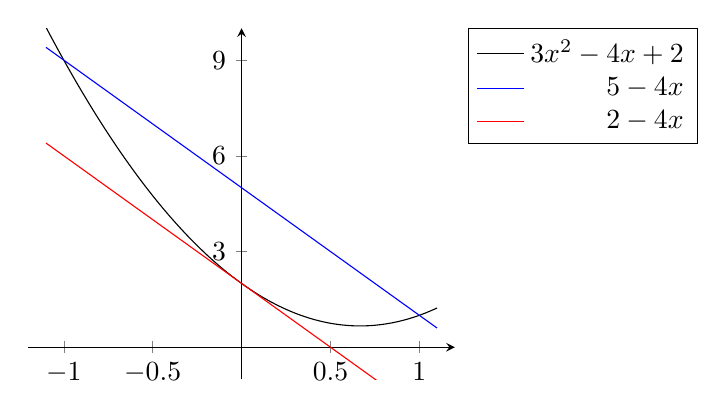
\begin{tikzpicture}
\begin{axis}[
  width=7cm,
  legend style={
    cells={anchor=east},
    legend pos=outer north east,
  },
  axis x line=center, axis y line=center,
  xmax=1.2,xmin=-1.2, xtick={-1,-0.5,0.5,1},
  ymin=-1, ymax=10,
  ytick={0,3,6,9},
  yticklabels={0,3,6,9}
  ]
\addplot[black,domain=-1.1:1.1,samples=100] {3*x*x-4*x+2}; \addlegendentry{$3x^2-4x+2$}
\addplot[blue,domain=-1.1:1.1,samples=100] {5-4*x};  \addlegendentry{$5-4x$}
\addplot[red,domain=-1.1:1.1,samples=100] {2-4*x};  \addlegendentry{$2-4x$}
\end{axis}
\end{tikzpicture}
\end{center}
\end{efig}
\end{itemize}

\end{eg}

\begin{eg}\label{eg:mvtg}
We can return to our initial car-motivated examples. Say you are driving along a straight
road in a car that can go at most $80km/h$. How far can you go in 2 hours? --- the answer
is easy, but we can also solve this using MVT.
\begin{itemize}
 \item Let $s(t)$ be the position of the car in $km$ at time $t$ measured in hours.
\item Then $s(0)=0$ and $s(2)=q$, where $q$ is the quantity that we need to bound.
\item We are told that $| s'(t) | \leq 80$, or equivalently
\begin{align*}
-80 \leq s'(t) \leq 80
\end{align*}
\item By the MVT there is some $c$ between 0 and 2 so that
\begin{align*}
  s'(c) &= \frac{q-0}{2} = \frac{q}{2}
\end{align*}
\item Now since $-80 \leq s'(c) \leq 80$ we must have $-80 \leq q/2 \leq 80$ and hence
$-160 \leq q=s(2) \leq 160$.
\end{itemize}
\end{eg}
More generally if we have some information about the derivative, then we can use the
MVT to leverage this information to tell us something about the function.
\begin{eg}\label{eg_2_13_4}
Let $f(x)$ be a differentiable function so that
\begin{align*}
  f(1)&=10 &\text{ and }&& -1 \leq f'(x) \leq 2 \text{ everywhere}
\end{align*}
Obtain upper and lower bounds on $f(5)$.


Okay --- what do we do?
\begin{itemize}
 \item Since $f(x)$ is differentiable we can use the MVT.
 \item Say $f(5)=q$, then the MVT tells us that there is some $c$ between $1$ and $5$ such
  that
\begin{align*}
 f'(c) &=\frac{q-10}{5-1} = \frac{q-10}{4}
\end{align*}
\item But we know that $-1 \leq f'(c) \leq 2$, so
\begin{align*}
-1 &\leq f'(c) \leq 2 \\
-1 & \leq \frac{q-10}{4} \leq 2 \\
  -4 & \leq q-10 \leq 8 \\
  6 \leq q \leq 18
\end{align*}
\item Thus we must have $6 \leq f(5) \leq 18$.
\end{itemize}
\end{eg}

\subsubsection*{(Optional) --- Why is the MVT True?}
We won't give a real proof for this theorem, but we'll look at a picture
which shows why it is true. Here is the picture. It contains a sketch of
the graph of $f(x)$, with $x$ running from $a$ to $b$, as well as
a line segment which is the secant of the graph from the point
$\big(a\,,f(a)\big)$ to the point $\big(b\,,f(b)\big)$. The slope of
the secant is exactly $\frac{f(b)-f(a)}{b-a}$.
\vadjust{
    \begin{efig}
    \begin{center}
       \includegraphics{mvtc}
    \end{center}
    \end{efig}
}
Remember that we are looking for a point, $\big(c\,,f(c)\big)$, on the
graph of $f(x)$ with the property that $f'(c)=\frac{f(b)-f(a)}{b-a}$,
i.e. with the property that the slope of the tangent line at
$\big(c\,,f(c)\big)$ is the same as the slope of the secant.
So imagine that you start moving the secant upward, carefully keeping
the moved line segment parallel to the secant. So the slope of the
moved line segment is always exactly  $\frac{f(b)-f(a)}{b-a}$.
When we first start moving the line segment it is not tangent to the curve ---
it crosses the curve. This is illustrated in the figure by the second line
segment from the bottom.
If we move the line segment too far it does not touch the curve at all.
This is illustrated in the figure by the top segment. But if we stop
moving the line segment just before it stops intersecting the curve at
all, we get exactly the tangent line to the curve at the point on the curve
that is farthest from the secant. This tangent line has exactly the desired
slope. This is illustrated in the figure by the third line
segment from the bottom.

\subsection*{Be Careful with Hypotheses}
\label{warning:mvt}
The mean value theorem has hypotheses --- $f(x)$ has to be continuous
for $a\le x\le b$ and has to be differentiable for $a<x<b$.
If either hypothesis is violated, the conclusion of the mean value theorem
can fail. That is, the curve $y=f(x)$ need not have a
tangent line at some $x=c$ between $a$ and $b$ whose slope, $f'(c)$,
is the same as the slope, $\frac{f(b)-f(a)}{b-a}$, of the secant joining
the points $\big(a\,,f(a)\big)$ and $\big(b\,,f(b)\big)$ on the
curve. If $f'(x)$ fails to exist for even a single value of $x$ between
$a$ and $b$, all bets are off. The following two examples illustrate this.

\begin{eg}\label{eg:mvtd}
For the first ``bad'' example, $a=0$, $b=2$ and
\smallskip
\begin{align*}
f(x) = \begin{cases}
           0  & \text{if }x \le 1 \\
           1 & \text{if }x>1
       \end{cases}
\hskip0.8in  \smash{\raisebox{-0.5\height}{\includegraphics{mvtd}}}
\end{align*}
\smallskip
\noindent
For this example, $f'(x)=0$ at every $x$ where it is defined. That is,
at every $x\ne 1$. But the slope of the secant joining
$\big(a\,,f(a)\big)=(0,0)$ and $\big(b\,,f(b)\big)=(2,1)$
is $\frac{1}{2}$.
\end{eg}


\begin{eg}\label{eg:mvte}
For the second ``bad''  example, $a=-1$, $b=1$ and $f(x)=|x|$.
For this function
\smallskip
\begin{align*}
f'(x) = \begin{cases}
           -1  & \text{if }x < 0 \\
            \text{undefined} & \text{if }x=0\\
           1 & \text{if }x>0
       \end{cases}
\hskip0.8in  \smash{\raisebox{-0.5\height}{\includegraphics{mvte}}}
\end{align*}
\smallskip
\noindent
For this example, $f'(x)=\pm 1$ at every $x$ where it is defined. That is,
at every $x\ne 0$. But the slope of the secant joining
$\big(a\,,f(a)\big)=(-1,1)$ and $\big(b\,,f(b)\big)=(1,1)$
is $0$.
\end{eg}


\begin{eg}\label{eg:mvtf}
Here is one ``good'' example, where the hypotheses of the mean value theorem
are satisfied. Let $f(x)=x^2$. Then $f'(x)=2x$. For any $a<b$,
\begin{align*}
\frac{f(b)-f(a)}{b-a}=\frac{b^2-a^2}{b-a}=b+a
\end{align*}
So $f'(c)=2c$ is exactly $\frac{f(b)-f(a)}{b-a}$ when $c=\frac{a+b}{2}$,
which, in this example, happens to be exactly half way between $x=a$ and
$x=b$.
    \begin{efig}
    \begin{center}
       \includegraphics{mvtf}
    \end{center}
    \end{efig}
\end{eg}

A simple consequence of the mean value theorem is that if you know the
sign of $f'(c)$ for all $c$'s between $a$ and $b$, with $b>a$, then
$f(b)-f(a) = f'(c) (b-a)$ must have the same sign.
\begin{cor}[Consequences of the mean value theorem]
\label{cor:DIFFmvtcons}
Let $A$ and $B$ be real numbers with $A<B$.
Let function $f(x)$ be defined and continuous on
the closed interval $A\le x\le B$ and be differentiable on the
open interval $A<x<B$.
\begin{enumerate}[(a)]
\item If $f'(c)=0$ for all $A<c<B$, then $f(b)=f(a)$ for all
$A\le a<b\le B$.\\
--- That is, $f(x)$ is constant on $A\le x\le B$.
\item If $f'(c)\ge 0$ for all $A<c<B$, then $f(b)\ge f(a)$ for all
$A\le a\le b\le B$.\\
--- That is, $f(x)$ is increasing on $A\le x\le B$.
\item If $f'(c)\le 0$ for all $A<c<B$, then $f(b)\le f(a)$ for all
$A\le a \le b\le B$.\\
--- That is, $f(x)$ is decreasing on $A\le x\le B$.
\end{enumerate}

\end{cor}
It is not hard to see why the above is true:
\begin{itemize}
 \item Say $f'(x)=0$ at every point in the interval $[A,B]$. Now pick any $a,b \in [A,B]$
with $a<b$. Then the MVT tells us that there is $c \in (a,b)$ so that
\begin{align*}
  f'(c) &= \frac{f(b)-f(a)}{b-a}
\end{align*}
If $f(b) \neq f(a)$ then we must have that $f'(c) \neq 0$ --- contradicting what we are
told about $f'(x)$. Thus we must have that $f(b)=f(a)$.

\item Similarly, say $f'(x) \geq 0$ at every point in the interval $[A,B]$. Now pick any
$a,b \in [A,B]$  with $a<b$. Then the MVT tells us that there is $c \in (a,b)$ so that
\begin{align*}
  f'(c) &= \frac{f(b)-f(a)}{b-a}
\end{align*}
Since $b>a$, the denominator is positive. Now if $f(b) < f(a)$ the numerator would be
negative, making the right-hand side negative, and contradicting what we are told about
$f'(x)$. Hence we must have $f(b)\ge f(a)$.
\end{itemize}

A nice corollary of the above corollary is the following:
\begin{cor}\label{cor equal diff}
If $f'(x) = g'(x)$ for all $x$ in the open interval $(a,b)$, then $f-g$ is a constant on
$(a,b)$. That is $f(x)=g(x)+c$, where $c$ is some constant.
\end{cor}
We can prove this by setting $h(x)=f(x)-g(x)$. Then $h'(x)=0$ and so the previous
corollary tells us that $h(x)$ is constant.

\begin{eg}\label{eg_2_13_5}
Using this corollary we can prove results like the following:
\begin{align*}
  \arcsin x + \arccos x &= \frac{\pi}{2} & \mbox{for all } -1 < x < 1
\end{align*}
How does this work? Let $f(x) = \arcsin x + \arccos x$. Then
\begin{align*}
  f'(x) &= \frac{1}{\sqrt{1-x^2}} + \frac{-1}{\sqrt{1-x^2}} = 0
\end{align*}
Thus $f$ must be a constant. To find out which constant, we can just check its value at a
convenient point, like $x=0$.
\begin{align*}
  \arcsin(0) + \arccos(0) &= \pi/2 + 0 = \pi/2
\end{align*}
Since the function is constant, this must be the value.
\end{eg}


%%%%%%%%%%%%%%%%%%%%%%%%%%%%%%%%%%%%%%%%%%%%%%
\section{Higher Order Derivatives}\label{sec higher diff}
%%%%%%%%%%%%%%%%%%%%%%%%%%%%%%%%%%%%%%%%%%%%%%

The operation of differentiation takes as input one function,
$f(x)$, and produces as output another function, $f'(x)$. Now $f'(x)$ is
once again a function. So we can differentiate it again, assuming that
it is differentiable, to create a third function, called the second
derivative of $f$. And we can differentiate the second derivative again
to create a fourth function, called the third derivative of $f$.
And so on.
\begin{notn}\label{not:higherOrdDeriv}
\begin{itemize}
\item $f''(x)$ and $f^{(2)}(x)$  and $\ddiff{2}{f}{x}(x)$ all mean
$\diff{}{x}\big(\diff{}{x}f(x)\big)$
\item $f'''(x)$ and $f^{(3)}(x)$  and $\ddiff{3}{f}{x}(x)$ all mean
$\diff{}{x}\big(\diff{}{x}\big(\diff{}{x}f(x)\big)\big)$
\item $f^{(4)}(x)$  and $\ddiff{4}{f}{x}(x)$ both mean
$\diff{}{x}\big(\diff{}{x}\big(\diff{}{x}\big(\diff{}{x}f(x)\big)\big)\big)$
\item and so on.
\end{itemize}
\end{notn}

Here is a simple example. Then we'll think a little about the significance
of second order derivatives. Then we'll do a more a computationally complex
example.

\begin{eg}\label{eg:higherOrdDerivA}
Let $n$ be a natural number and let $f(x)= x^n$. Then
\begin{align*}
\diff{}{x}x^n&=nx^{n-1} \\
\ddiff{2}{}{x}x^n&=\diff{}{x}\big(nx^{n-1}\big)=n(n-1)x^{n-2} \\
\ddiff{3}{}{x}x^n&=\diff{}{x}\big(n(n-1)x^{n-2}\big)=n(n-1)(n-2)x^{n-3}
\end{align*}
Each time we differentiate, we bring down the exponent, which is exactly
one smaller than the previous exponent brought down, and we reduce the
exponent by one. By the time we have differentiated $n-1$ times,
the exponent has decreased to $n-(n-1)=1$ and we have brought down the
factors $n(n-1)(n-2)\cdots 2$. So
\begin{align*}
\ddiff{{n-1}}{}{x}x^n&=n(n-1)(n-2)\cdots 2x
\end{align*}
and
\begin{align*}
\ddiff{n}{}{x}x^n&=n(n-1)(n-2)\cdots 1
\end{align*}
The product of the first $n$ natural numbers, $1\cdot 2\cdot 3\cdot \cdots
\cdot n,$ is called ``$n$ factorial'' and is denoted $n!$. So we can also
write
\begin{align*}
\ddiff{n}{}{x}x^n&=n!
\end{align*}
If $m>n$, then
\begin{align*}
\ddiff{m}{}{x}x^n&=0
\end{align*}
\end{eg}

\begin{eg}\label{eg_2_14_1}
Recall that the derivative $v'(a)$ is the (instantaneous) rate of
change of the function $v(t)$ at $t=a$. Suppose that you are walking on
the $x$--axis and that $x(t)$ is your $x$--coordinate at time $t$.
Also suppose, for simplicity, that you are moving from left to right.
Then $v(t)=x'(t)$ is your velocity at time $t$ and $v'(a)=x''(a)$ is the
rate at which your velocity is changing at time $t=a$. It is called your
acceleration. In particular, if $x''(a)>0$, then your velocity is increasing,
i.e. you are speeding up, at time $a$. If $x''(a)<0$, then your velocity
is decreasing, i.e. you are slowing down, at time $a$. That's one
interpretation of the second derivative.
\end{eg}

\begin{eg}[Example \ref{eg:DIFFimpldiffD}, continued]\label{eg:higherOrdDerivC}
Find $y''$ if $y=y^3+xy+x^3$.

\soln This problem concerns some function $y(x)$ that is not
given to us explicitly. All that we are told is that $y(x)$ satisfies
\begin{equation}
y(x)=y(x)^3+xy(x)+x^3
\tag{E1}
\end{equation}
for all $x$. We are asked to find $y''(x)$. We cannot solve this
equation to get an explicit formula for $y(x)$.  So we use implicit
differentiation, as we did in Example \ref{eg:DIFFimpldiffD}. That is, we apply
$\diff{}{x}$ to both sides of (E1). This gives
\begin{equation}
y'(x)=3y(x)^2\,y'(x)+y(x)+x\,y'(x)+3x^2
%\implies \big[1-x-3y(x)^2\big]y'(x) = y(x)+3x^2
\tag{E2}
\end{equation}
which we can solve for $y'(x)$, by moving all $y'(x)$'s to the left hand
side, giving
\begin{equation*}
 \big[1-x-3y(x)^2\big]y'(x) = y(x)+3x^2
\end{equation*}
and then dividing across.
\begin{equation}
y'(x) = \frac{y(x)+3x^2}{1-x-3y(x)^2}
\tag{E3}\end{equation}
To get $y''(x)$, we have two options.

\noindent\emph{Method 1.}\ \ \  Apply $\diff{}{x}$ to both sides of (E2).
This gives
\begin{equation*}
y''(x)=3y(x)^2\,y''(x)+6y(x)\,y'(x)^2+2y'(x)+x\,y''(x)+6x
\end{equation*}
We can now solve for $y''(x)$, giving
\begin{equation}
y''(x) = \frac{6x+2y'(x)+6y(x)y'(x)^2}{1-x-3y(x)^2}
\tag{E4}
\end{equation}
Then we can substitute in (E3), giving
\begin{align*}
y''(x) &= 2\frac{3x+ \frac{y(x)+3x^2}{1-x-3y(x)^2}
              +3y(x) \big(\frac{y(x)+3x^2}{1-x-3y(x)^2}\big)^2}
         {1-x-3y(x)^2} \\
&= 2\frac{3x{[1-x-3y(x)^2]}^2+ [y(x)+3x^2][1-x-3y(x)^2]
              +3y(x) {[y(x)+3x^2]}^2}{{[1-x-3y(x)^2]}^3}
\end{align*}

\noindent\emph{Method 2.}\ \ \  Alternatively, we can also differentiate (E3).
\begin{align*}
y''(x) &= \frac{[y'(x)+6x][1-x-3y(x)^2]-
           [y(x)+3x^2][-1-6y(x)y'(x)]}{{[1-x-3y(x)^2]}^2} \\[0.05in]
&= \frac{[\frac{y(x)+3x^2}{1-x-3y(x)^2}+6x][1-x-3y(x)^2]-
           [y(x)+3x^2][-1-6y(x)\frac{y(x)+3x^2}{1-x-3y(x)^2}]}
                                       {{[1-x-3y(x)^2]}^2}\\[0.05in]
&= \frac{2[y(x)+3x^2][1-x-3y(x)^2]+6x{[1-x-3y(x)^2]}^2
           +6y(x){[y(x)+3x^2]}^2}
                                       {{[1-x-3y(x)^2]}^3}
\end{align*}

\noindent\emph{Remark 1.}\ \ \ We have now computed $y''(x)$ --- sort of.
The answer is in terms of $y(x)$, which we don't know. Since we cannot
get an explicit formula for $y(x)$, there's not a great deal that we can do,
in general.

\noindent\emph{Remark 2.}\ \ \ Even though we cannot solve
$y=y^3+xy+x^3$ explicitly for $y(x)$, for general $x$, it is sometimes
possible to solve equations like this for some special values of $x$.
In fact, we saw in Example \ref{eg:DIFFimpldiffD} that when $x=1$,
the given equation reduces to $y(1)=y(1)^3+1\cdot y(1)+1^3$, or $y(1)^3=-1$,
which we can solve to get $y(1)=-1$. Substituting into (E2),
as we did in  Example \ref{eg:DIFFimpldiffD} gives
\begin{equation*}
y'(1) = \frac{-1+3}{1-1-3(-1)^2} = -\frac{2}{3}
\end{equation*}
and substituting into (E4) gives
\begin{equation*}
y''(1) = \frac{6+2\big(-\frac{2}{3}\big)+6(-1)\big(-\frac{2}{3}\big)^2}
                             {1-1-3(-1)^2}
   =\frac{6-\frac{4}{3}-\frac{8}{3}}{-3}
   = -\frac{2}{3}
\end{equation*}
(It's a fluke that, in this example, $y'(1)$ and $y''(1)$ happen to be equal.)
So we now know that, even though we can't solve $y=y^3+xy+x^3$ explicitly for
$y(x)$, the graph of the solution passes through $(1,-1)$ and has slope
$-\frac{2}{3}$ (i.e. is sloping downwards by between $30^\circ$ and $45^\circ$)
there and, furthermore, the slope of the graph decreases as $x$
increases through $x=1$.

\begin{efig}
 \begin{center}
 \includegraphics{concaveDown}
 \end{center}
\end{efig}
Here is a sketch of the part of the graph very near $(1, -1)$. The tangent line to the
graph at $(1, -1)$ is also shown. Note that the tangent line is sloping down to the right,
as we expect, and that the graph lies below the tangent line near $(1,-1)$. That's because
the slope $f'(x)$ is decreasing (becoming more negative) as $x$ passes through $1$.


\end{eg}

\begin{warning}\label{warning:dropx}
Many people will suppress the $(x)$ in $y(x)$ when doing
computations like those in Example \ref{eg:higherOrdDerivC}.
This gives shorter, easier to read formulae, like
$y'=\frac{y+3x^2}{1-x-3y^2}$. If you do this, you must never forget
that $y$ is a function of $x$ and is \emph{not} a constant. If you do forget,
you'll make the very serious error of saying that $\diff{y}{x}=0$,
which is false.

\end{warning}


\section{(Optional) --- Is $\lim\limits_{x\to c}f'(x)$ Equal to $f'(c)$?}\label{sec:cont_deriv}

Consider the function
\begin{equation*}
f(x) = \begin{cases}
            \frac{\sin x^2}{x} &\text{if $x\ne 0$} \\
             0                  &\text{if $x=0$}
        \end{cases}
\end{equation*}
For any $x\ne 0$ we can easily use our differentiation rules to find
\begin{align*}
f'(x) = \frac{2x^2\cos x^2 -\sin x^2}{x^2}
\end{align*}
But for $x=0$ none of our usual differentation rules apply. So how do we find $f'(0)$? One obviously legitimate strategy is to directly apply the 
Definition \ref{def:DIFFderiv}
of the derivative. As an alternative, we will now consider the question ``Can one find $f'(0)$ by taking the limit of $f'(x)$ as $x$ tends to zero?''.
There is bad news and there is good news.
\begin{itemize}
\item
The bad news is that,
even for functions $f(x)$ that are differentiable for all $x$, $f'(x)$ need not be continuous. That is, it is \emph{not} always true that 
$\lim_{x\rightarrow 0}f'(x) = f'(0)$. We will see a function for which 
$\lim_{x\rightarrow 0}f'(x) \ne f'(0)$ in 
Example \ref{eg:discontinuous derivative}, below.
\item
The good news is that Theorem \ref{thm:continuous derivative}, below 
provides conditions which are sufficient to guarantee that $f(x)$ is differentiable at $x=0$ and that $\lim_{x\rightarrow 0}f'(x) = f'(0)$.  
\end{itemize}



\begin{eg}\label{eg:discontinuous derivative}
Consider the function
\begin{equation*}
f(x) = \begin{cases}
            x^2\sin\frac{1}{x} &\text{if $x\ne 0$} \\
             0                  &\text{if $x=0$}
        \end{cases}
\end{equation*}
For $x\ne 0$ we have, by the product and chain rules,
\begin{align*}
f'(x)  &= 2x\, \sin\frac{1}{x} + x^2 \left(\cos\frac{1}{x}\right)
                     \left(-\frac{1}{x^2}\right) \\
       &=  2x\, \sin\frac{1}{x} - \cos\frac{1}{x}
\end{align*}
As $\left|\sin\frac{1}{x}\right|\le 1$, we have
\begin{equation*}
\lim_{x\rightarrow 0}2x\, \sin\frac{1}{x}=0
\end{equation*}
On the other hand, as $x$ tends to zero, $\frac{1}{x}$ goes to $\pm\infty$.
So
\begin{equation*}
\lim_{x\rightarrow 0}\cos\frac{1}{x} = DNE
\implies 
\lim_{x\rightarrow 0}f'(x) = DNE
\end{equation*}
We will now see that, despite this, $f'(0)$ is perfectly well defined.
By definition
\begin{align*}
f'(0) &= \lim_{h\to 0}\frac{f(h)-f(0)}{h}  \\
      & = \lim_{h\to 0}\frac{h^2\sin\frac{1}{h}-0}{h} \\
      & = \lim_{h\to 0} h\sin\frac{1}{h} \\
      & = 0\qquad\text{since $\left|\sin\frac{1}{h}\right|\le 1$}
\end{align*}
So $f'(0)$ exists, but is not equal to $\lim_{x\rightarrow 0}f'(x)$,
which does not exist.
\end{eg}
Now for the good news.
%%%%%%%%%%%%%%%
\begin{theorem}\label{thm:continuous derivative}
Let $a<c<b$. Assume that 
\begin{itemize}
\item 
the function $f(x)$ is continous on the interval $a<x<b$ and
\item
is differentiable at every $x$ in the intervals $a<x<c$ and $c<x<b$ and
\item
the limit  $\lim_{x\rightarrow c}f'(x)$ exists.
\end{itemize}
Then $f$ is differentiable at $x=c$ and
\begin{equation*}
f'(c) = \lim_{x\rightarrow c}f'(x)
\end{equation*}
\end{theorem}

\begin{proof}
By hypothesis, there is a number $L$ such that
\begin{equation*}
\lim_{x\rightarrow c}f'(x) = L
\end{equation*}
By definition
\begin{equation*}
f'(c) = \lim_{h\to 0}\frac{f(c+h)-f(c)}{h}
\end{equation*}
By the Mean Value Theorem (Theorem \ref{thm:DIFFmvt}) 
there is, for each $h$,
an (unknown) number $x_h$ between $c$ and $c+h$ such that 
$f'(x_h)=\frac{f(c+h)-f(c)}{h}$. So
\begin{equation*}
f'(c) = \lim_{h\to 0} f'(x_h)
\end{equation*}
As $h$ tends to zero, $c+h$ tends to $c$, and so  $x_h$ is forced to tend 
to $c$, and $f'(x_h)$ is forced to tend to $L$ so that
\begin{equation*}
f'(c) = \lim_{h\to 0} f'(x_h) = L
\end{equation*}
\end{proof}


In the next example we evaluate $f'(0)$ by applying 
Theorem \ref{thm:continuous derivative}.
\begin{eg}\label{eg:continuous derivative}
Let 
\begin{equation*}
f(x) = \begin{cases}
            \frac{\sin x^2}{x} &\text{if $x\ne 0$} \\
             0                  &\text{if $x=0$}
        \end{cases}
\end{equation*}
We have already observed above that, for $x\ne 0$,
\begin{align*}
f'(x) = \frac{2x^2\cos x^2 -\sin x^2}{x^2}
      = 2\cos x^2 - \frac{\sin x^2}{x^2}
\end{align*}
We use Theorem~\ref{thm:continuous derivative} with $c=0$ to show that $f(x)$ is differentiable at $x=0$ and to evaluate $f'(0)$. That theorem 
has two hypotheses that we have not yet verified, namely the continuity of 
$f(x)$ at $x=0$, and the existence of the limit $\lim_{x\rightarrow 0}f'(x)$.
We verify them now.
\begin{itemize}
\item We already know, by Lemma \ref{lem sinhoverh},
that $\lim_{h\rightarrow 0}\frac{\sin h}{h}=1$. So
\begin{align*}
\lim_{x\rightarrow 0}\frac{\sin x^2}{x^2} 
&=\lim_{h\rightarrow 0^+}\frac{\sin h}{h}\qquad\text{with $h=x^2$} \\
&=1
\end{align*}
and
\begin{align*}
\lim_{x\rightarrow 0} f(x) 
&=\lim_{x\rightarrow 0}\frac{\sin x^2}{x}
=\lim_{x\rightarrow 0}x\,\frac{\sin x^2}{x^2}
=\lim_{x\rightarrow 0}x\ \lim_{x\rightarrow 0}\frac{\sin x^2}{x^2}
=0\times 1
=0
\end{align*}
and $f(x)$ is continuous at $x=0$.
\item The limit of the derivative is
\begin{align*}
\lim_{x\rightarrow 0}f'(x) 
&= \lim_{x\rightarrow 0}\left[2\cos x^2 - \frac{\sin x^2}{x^2}\right]
=2\times 1 -1 = 1
\end{align*}
\end{itemize}
So, by Theorem~\ref{thm:continuous derivative}, $f(x)$ is differentiable 
at $x=0$ and $f'(0)=1$.
\end{eg}





\begin{comment}


%%%%%%%%%%%%%%%%%%%%%%%%%%%%%%%%%%%%%%%%%%%%%%
\section{Higher Order Derivatives}
%%%%%%%%%%%%%%%%%%%%%%%%%%%%%%%%%%%%%%%%%%%%%%

The operation of differentiation takes as input one function,
$f(x)$, and produces as output another function, $f'(x)$. Now $f'(x)$ is
once again a function. So we can differentiate it again, assuming that
it is differentiable, to create a third function, called the second
derivative of $f$. And we can differentiate the second derivative again
to create a fourth function, called the third derivative of $f$.
And so on.
\begin{notn}\label{not:higherOrdDeriv}
\begin{itemize}
\item $f''(x)$ and $f^{(2)}(x)$  and $\ddiff{2}{f}{x}(x)$ all mean
$\diff{}{x}\big(\diff{}{x}f(x)\big)$
\item $f'''(x)$ and $f^{(3)}(x)$  and $\ddiff{3}{f}{x}(x)$ all mean
$\diff{}{x}\big(\diff{}{x}\big(\diff{}{x}f(x)\big)\big)$
\item $f^{(4)}(x)$  and $\ddiff{4}{f}{x}(x)$ both mean
$\diff{}{x}\big(\diff{}{x}\big(\diff{}{x}\big(\diff{}{x}f(x)\big)\big)\big)$
\item and so on.
\end{itemize}
\end{notn}

Here is a simple example. Then we'll think a little about the significance
of second order derivatives. Then we'll do a more a computationally complex example.

\begin{eg}\label{eg:higherOrdDerivA}
Let $n$ be a natural number and let $f(x)= x^n$. Then
\begin{align*}
\diff{}{x}x^n&=nx^{n-1} \\
\ddiff{2}{}{x}x^n&=\diff{}{x}\big(nx^{n-1}\big)=n(n-1)x^{n-2} \\
\ddiff{3}{}{x}x^n&=\diff{}{x}\big(n(n-1)x^{n-2}\big)=n(n-1)(n-2)x^{n-3}
\end{align*}
Each time we differentiate, we bring down the exponent, which is exactly
one smaller than the previous exponent brought down, and we reduce the
exponent by one. By the time we have differentiated $n-1$ times,
the exponent has decreased to $n-(n-1)=1$ and we have brought down the
factors $n(n-1)(n-2)\cdots 2$. So
\begin{align*}
\ddiff{{n-1}}{}{x}x^n&=n(n-1)(n-2)\cdots 2x
\end{align*}
and
\begin{align*}
\ddiff{n}{}{x}x^n&=n(n-1)(n-2)\cdots 1
\end{align*}
The product of the first $n$ natural numbers, $1\cdot 2\cdot 3\cdot \cdots
\cdot n,$ is called ``$n$ factorial'' and is denoted $n!$. So we can also
write
\begin{align*}
\ddiff{n}{}{x}x^n&=n!
\end{align*}
If $m>n$, then
\begin{align*}
\ddiff{m}{}{x}x^n&=0
\end{align*}
\end{eg}

Recall that the derivative $v'(a)$ is the (instantaneous) rate of
change of the function $v(t)$ at $t=a$. Suppose that you are walking on
the $x$--axis and that $x(t)$ is your $x$--coordinate at time $t$.
Also suppose, for simplicity, that you are moving from left to right.
Then $v(t)=x'(t)$ is your speed at time $t$ and $v'(a)=x''(a)$ is the
rate at which your speed is changing at time $t=a$. It is called your
acceleration. In particular, if $x''(a)>0$, then your speed is increasing,
i.e. you are speeding up, at time $a$. If $x''(a)<0$, then your speed
is decreasing, i.e. you are slowing down, at time $a$. That's one
interpretation of the second derivative.

Here is another interpretation. Consider the graph $y=f(x)$. Then we know
that $f'(x)$ is the slope of the (tangent line to the) graph at the point
$\big(x\,,\,f(x)\big)$. So $f''(a)$ is the rate at which the slope
at $\big(x\,,\,f(x)\big)$ is changing as $x$ increases through $a$.
If $f''(a)>0$ then the slope is increasing as you move from left to right
through $x=a$. In this case the curve is said to be concave up at $x=a$.
If $f''(a)<0$ then the slope is decreasing as you move from left to right
through $x=a$. In this case the curve is said to be concave down at $x=a$.
Here is a simple example, with a sketch, illustrating this.

\begin{eg}\label{eg:higherOrdDerivB}
Consider the graph $y=f(x)=x^3-3x$. The first two derivatives of the function
$f(x)$ are
\begin{equation*}
f'(x) = 3x^2-3=3(x^2-1)\qquad
f''(x) = 6x
\end{equation*}
So $f'(x)$ is strictly positive when $x^2>1$ (i.e. $x<-1$ or $x>1$),
zero when $x^2=1$ (i.e. $x=\pm 1$) and strictly negative when $x^2<1$
(i.e. $-1<x<1$). And $f''(x)$ is strictly positive when $x>0$,
zero when $x=0$ and strictly negative when $x<0$.
\begin{itemize}
\item When $x<-1$ the graph has positive slope but that slope decreases
(i.e. the tangent line becomes less steep) as $x$ increases. The graph
is concave down.
\item When $-1<x<0$ the graph has negative slope and that slope decreases
(i.e. becomes more negative -- the tangent line becomes steeper) as
$x$ increases. The graph is still concave down.
\item When $0<x<1$ the graph has negative slope but that slope increases
(i.e. becomes less negative -- the tangent line becomes less steep) as
$x$ increases. The graph is concave up.
\item When $x>1$ the graph has positive slope and that slope increases
as $x$ increases. The graph is concave up.
\end{itemize}
Here is a figure containing the graph and some tangent lines near $x=-1$
and near $x=+1$. We see the slope of the tangent lines
decreasing from a positive number through zero to a negative number as
$x$ increases through $-1$. And we see the slope of the tangent lines
increasing from a negative number through zero to a positive number as
$x$ increases through $+1$.

\begin{efig}
 \begin{center}
 \includegraphics{concaveUpDown}
 \end{center}
\end{efig}

\end{eg}


Now here is a more computationally complex example.

\begin{eg}[Example \ref{eg:DIFFimpldiffD}, continued]\label{eg:higherOrdDerivC}
Find $y''$ if $y=y^3+xy+x^3$.

\soln This problem concerns some function $y(x)$ that is not
given to us explicitly. All that we are told is that $y(x)$ satisfies
\begin{equation}\label{eq:hoDerivBa}
y(x)=y(x)^3+xy(x)+x^3
\end{equation}
for all $x$. We are asked to find $y''(x)$. We cannot solve this
equation to get an explicit formula for $y(x)$.  So we use implicit
differentiation, as we did in Example \ref{eg:DIFFimpldiffD}. That is, we apply
$\diff{}{x}$ to both sides of \eqref{eq:hoDerivBa}. This gives
\begin{equation}\label{eq:hoDerivBb}
y'(x)=3y(x)^2\,y'(x)+y(x)+x\,y'(x)+3x^2
%\implies \big[1-x-3y(x)^2\big]y'(x) = y(x)+3x^2
\end{equation}
which we can solve for $y'(x)$, by moving all $y'(x)$'s to the left hand
side, giving
\begin{equation*}
 \big[1-x-3y(x)^2\big]y'(x) = y(x)+3x^2
\end{equation*}
and then dividing across.
\begin{equation}\label{eq:hoDerivBc}
y'(x) = \frac{y(x)+3x^2}{1-x-3y(x)^2}
\end{equation}
To get $y''(x)$, we have two options.

\noindent\emph{Method 1.}\ \ \  Apply $\diff{}{x}$ to both sides of \eqref{eq:hoDerivBb}.
This gives
\begin{equation*}
y''(x)=3y(x)^2\,y''(x)+6y(x)\,y'(x)^2+2y'(x)+x\,y''(x)+6x
\end{equation*}
We can now solve for $y''(x)$, giving
\begin{equation}\label{eq:hoDerivBd}
y''(x) = \frac{6x+2y'(x)+6y(x)y'(x)^2}{1-x-3y(x)^2}
\end{equation}
Then we can substitute in \eqref{eq:hoDerivBc}, giving
\begin{align*}
y''(x) &= 2\frac{3x+ \frac{y(x)+3x^2}{1-x-3y(x)^2}
              +3y(x) \big(\frac{y(x)+3x^2}{1-x-3y(x)^2}\big)^2}
         {1-x-3y(x)^2} \\
&= 2\frac{3x{[1-x-3y(x)^2]}^2+ [y(x)+3x^2][1-x-3y(x)^2]
              +3y(x) {[y(x)+3x^2]}^2}{{[1-x-3y(x)^2]}^3}
\end{align*}

\noindent\emph{Method 2.}\ \ \  Alternatively, we can also differentiate
\eqref{eq:hoDerivBc}.
\begin{align*}
y''(x) &= \frac{[y'(x)+6x][1-x-3y(x)^2]-
           [y(x)+3x^2][-1-6y(x)y'(x)]}{{[1-x-3y(x)^2]}^2} \\[0.05in]
&= \frac{[\frac{y(x)+3x^2}{1-x-3y(x)^2}+6x][1-x-3y(x)^2]-
           [y(x)+3x^2][-1-6y(x)\frac{y(x)+3x^2}{1-x-3y(x)^2}]}
                                       {{[1-x-3y(x)^2]}^2}\\[0.05in]
&= \frac{2[y(x)+3x^2][1-x-3y(x)^2]+6x{[1-x-3y(x)^2]}^2
           +6y(x){[y(x)+3x^2]}^2}
                                       {{[1-x-3y(x)^2]}^3}
\end{align*}

\noindent\emph{Remark 1.}\ \ \ We have now computed $y''(x)$ --- sort of.
The answer is in terms of $y(x)$, which we don't know. Since we cannot
get an explicit formula for $y(x)$, there's not a great deal that we can do,
in general.

\noindent\emph{Remark 2.}\ \ \ Even though we cannot solve
$y=y^3+xy+x^3$ explicitly for $y(x)$, for general $x$, it is sometimes
possible to solve equations like this for some special values of $x$.
In fact, we saw in Example \ref{eg:DIFFimpldiffD} that when $x=1$,
the given equation reduces to $y(1)=y(1)^3+1\cdot y(1)+1^3$, or $y(1)^3=-1$,
which we can solve to get $y(1)=-1$. Substituting into \eqref{eq:hoDerivBb},
as we did in  Example \ref{eg:DIFFimpldiffD} gives
\begin{equation*}
y'(1) = \frac{-1+3}{1-1-3(-1)^2} = -\frac{2}{3}
\end{equation*}
and substituting into \eqref{eq:hoDerivBd} gives
\begin{equation*}
y''(1) = \frac{6+2\big(-\frac{2}{3}\big)+6(-1)\big(-\frac{2}{3}\big)^2}
                             {1-1-3(-1)^2}
   =\frac{6-\frac{4}{3}-\frac{8}{3}}{-3}
   = -\frac{2}{3}
\end{equation*}
(It's a fluke that, in this example, $y'(1)$ and $y''(1)$ happen to be equal.)
So we now know that, even though we can't solve $y=y^3+xy+x^3$ explicitly for
$y(x)$, the graph of the solution passes through $(1,-1)$ and has slope
$-\frac{2}{3}$ (i.e. is sloping downwards by between $30^\circ$ and $45^\circ$)
there and, furthermore, the slope of the graph decreases as $x$
increases through $x=1$.  The graph is concave down near $x=1$. Here
is a sketch of the part of the graph very near $(1,-1)$. The tangent
line to the graph at $(1,-1)$ is also shown. Note that the tangent line
is sloping down to the right, as we expect, and that the graph lies below
the tangent line near $(1,-1)$. That is typical of concave down graphs.

\begin{efig}
 \begin{center}
 \includegraphics{concaveDown}
 \end{center}
\end{efig}


\end{eg}

\begin{warning}\label{warning:dropx}
Many people will suppress the $(x)$ in $y(x)$ when doing
computations like those in Example \ref{eg:higherOrdDerivC}.
This gives shorter, easier to read formulae, like
$y'=\frac{y+3x^2}{1-x-3y^2}$. If you do this, you must never forget
that $y$ is a function of $x$ and is \emph{not} a constant. If you do forget,
you'll make the very serious error of saying that $\diff{y}{x}=0$,
which is false.

\end{warning}


\intremark{ %%%% INTERNAL REMARK - another, less good, example
\begin{eg}\label{eg:higherOrdDerivNU}
Find $y''$ if $4y+x^4+y^4=6$.

\soln This problem concerns some function $y(x)$ that is not
given to us explicitly. All that we are told is that $y(x)$ satisfies
\begin{equation}\label{eq:hoDerivBa}
4y(x) +x^4+y(x)^4=6
\end{equation}
for all $x$. We are asked to find $y''(x)$. We cannot solve this
equation to get an explicit formula for $y(x)$.  So we use implicit
differentiation, as we did in Example \ref{eg:DIFFimpldiffD}. That is, we apply
$\diff{}{x}$ to both sides of \eqref{eq:hoDerivBa}. This gives
\begin{equation}\label{eq:hoDerivBb}
4y'(x) +4x^3+4y(x)^3y'(x)=0
\implies y'(x) +x^3+y(x)^3y'(x)=0
\end{equation}
which we can solve for $y'(x)$.
\begin{equation}\label{eq:hoDerivBc}
y'(x) = -\frac{x^3}{1+y(x)^3}
\end{equation}
To get $y''(x)$, we have two options.

\noindent\emph{Method 1.}\ \ \  Apply $\diff{}{x}$ to both sides of \eqref{eq:hoDerivBb}.
This gives
\begin{equation}\label{eq:hoDerivBd}
y''(x) +3x^2+3y(x)^2y'(x)^2+y(x)^3y''(x)=0
\end{equation}
We can now solve for $y''(x)$, giving
\begin{equation*}
y''(x) = -\frac{3x^2+3y(x)^2y'(x)^2}{1+y(x)^3}
\end{equation*}
and then substitute in \eqref{eq:hoDerivBc}, giving
\begin{equation*}
y''(x) = -3\frac{x^2+y(x)^2\frac{x^6}{{[1+y(x)^3]}^2}}{1+y(x)^3}
= -3\frac{x^2{[1+y(x)^3]}^2+y(x)^2x^6}{{[1+y(x)^3]}^3}
\end{equation*}

\noindent\emph{Method 2.}\ \ \  Alternatively, we can also differentiate
\eqref{eq:hoDerivBc}.
\begin{align*}
y''(x) &= -\frac{3x^2[1+y(x)^3]-x^3\,3y(x)^2y'(x)}{{[1+y(x)^3]}^2}
= -\frac{3x^2[1+y(x)^3]+x^3\,3y(x)^2\frac{x^3}{1+y(x)^3}}{{[1+y(x)^3]}^2}\\
&= -3\frac{x^2{[1+y(x)^3]}^2+y(x)^2x^6}{{[1+y(x)^3]}^3}
\end{align*}

\noindent\emph{Remark 1.}\ \ \ We have now computed $y''(x)$ --- sort of.
The answer is in terms of $y(x)$, which we don't know. Since we cannot
get an explicit formula for $y(x)$, there's not a great deal that we can do.

%\noindent\emph{Remark 2.}\ \ \ Even though we cannot solve
%$4y(x) +x^4+y(x)^4=6$ explicitly for $y(x)$, for general $x$, it is sometimes
%possible to solve equations like this for some special values of $x$.
%For example, when $x=1$, the equation reduces to
%\begin{equation*}
%4y(1) + y(1)^4=5
%\end{equation*}
\end{eg}
}  %%% END INTERNAL REMARK - another, less good, example


%%%%%%%%%%%%%%%%%%%%%%%%%%%%%%%%%%%%%%%%%%%%%%
\section{Approximating Functions Near a Specified Point --- Taylor
Polynomials}\label{sec:DIFFTaylor}
%%%%%%%%%%%%%%%%%%%%%%%%%%%%%%%%%%%%%%%%%%%%%5
Suppose that you are interested in the values of some function $f(x)$ for
$x$ near some fixed point $a$. The function is too complicated to work
with directly. So you wish to work instead with some other function $F(x)$
that is both simple and a good approximation to $f(x)$ for $x$ near
$a$. We'll consider a couple of examples of this scenario later.
First, we develop several different approximations.

%%%%%%%%%%%%%%%%%%%%%%%%%%%%%%%%%%%%%%%%%%%%%%%%%%%%%%%%%%%%%%%%%%%%%%
\subsection{Zeroth Approximation --- the Constant Approximation}
%%%%%%%%%%%%%%%%%%%%%%%%%%%%%%%%%%%%%%%%%%%%%%%%%%%%%%%%%%%%%%%%%%%%%%
The simplest functions are those that are constants. The first
approximation will be by a constant function. That is, the approximating
function will have the form $F(x)=A$, for some constant $A$. To ensure
that $F(x)$ is a good approximation for $x$ close to $a$, we choose
$A$ so that $f(x)$ and $F(x)$ take exactly the same value when $x=a$.
\begin{equation*}
F(x)=A\qquad\text{so}\qquad F(a)=A=f(a)\implies A=f(a)
\end{equation*}
Our first, and crudest, approximation rule is
\begin{equation}\label{eq:constApprox}
f(x)\approx f(a)
\end{equation}
Here is a figure showing the graphs of a typical $f(x)$ and approximating
function $F(x)$.
\vadjust{
    \begin{efig}
    \begin{center}
       \includegraphics{approx1}
    \end{center}
    \end{efig}
}
At $x=a$, $f(x)$ and $F(x)$ take the same value. For $x$ very near $a$,
the values of $f(x)$ and $F(x)$ remain close together. But the quality
of the approximation deteriorates fairly quickly as $x$ moves
away from $a$.

%%%%%%%%%%%%%%%%%%%%%%%%%%%%%%%%%%%%%%%%%%%%%%%%%%%%%%%%%%%%%%%%%%%%%%
\subsection{First Approximation --- the Tangent Line, or Linear, Approximation}
%%%%%%%%%%%%%%%%%%%%%%%%%%%%%%%%%%%%%%%%%%%%%%%%%%%%%%%%%%%%%%%%%%%%%%
We now develop a better approximation by allowing the approximating function
to be a linear function of $x$ and not just a constant function. That is,
we allow $F(x)$ to be of the form $A+Bx$, for some constants $A$ and $B$.
To ensure that $F(x)$ is a good approximation for $x$ close to $a$,
we choose $A$ and $B$  so that $f(a)=F(a)$ and $f'(a)=F'(a)$.
Then $f(x)$ and $F(x)$ will have both the same value and the same
slope at $x=a$.
\begin{align*}
F(x)&=A+Bx  & &\implies & F(a)=A+Ba&=f(a)\\
F'(x)&=B    & &\implies & F'(a)=\phantom{A+a}B&=f'(a)
\end{align*}
Substituting $B=f'(a)$ into $A+Ba=f(a)$ gives
$A=f(a)-af'(a)$ and consequently $F(x)=A+Bx=f(a)-af'(a)+xf'(a)
=f(a)+f'(a)(x-a)$. So, our second approximation is
\begin{equation}\label{eq:linApprox}
f(x)\approx f(a)+f'(a)(x-a)
\end{equation}
Recall, from Theorem \ref{thm:DIFFtangentLine}, that $y=f(a)+f'(a)(x-a)$
is exactly the equation of the tangent line to the curve $y=f(x)$ at $a$.
Here is a figure showing the graphs of a typical $f(x)$ and approximating
function $F(x)$.
\vadjust{
    \begin{efig}
    \begin{center}
       \includegraphics{approx2}
    \end{center}
    \end{efig}
}
Observe that the graph of $f(a)+f'(a)(x-a)$ remains close to the
graph of $f(x)$ for a much larger range of $x$ than did the graph of $f(a)$.
%%%%%%%%%%%%%%%%%%%%%%%%%%%%%%%%%%%%%%%%%%%%%%%%%%%%%%%%%%%%%%%%%%%%%%
\subsection{Second Approximation --- the Quadratic Approximation}
%%%%%%%%%%%%%%%%%%%%%%%%%%%%%%%%%%%%%%%%%%%%%%%%%%%%%%%%%%%%%%%%%%%%%%

We next develop a still better approximation by allowing the
approximating function be to a quadratic function of $x$. That is,
we allow $F(x)$ to be of the form $A+Bx+Cx^2$, for some constants $A$, $B$
and $C$. To ensure that $F(x)$ is a good approximation for $x$ close
to $a$, we choose $A$, $B$ and $C$ so that $f(a)=F(a)$
and $f'(a)=F'(a)$ and $f''(a)=F''(a)$.
\begin{align*}
F(x)&=A+Bx+Cx^2  & &\implies & F(a)=A+Ba+\phantom{2}Ca^2&=f(a)\\
F'(x)&=B+2Cx & &\implies & F'(a)=\phantom{A+a}B+2Ca&=f'(a)\\
F''(x)&=2C   & &\implies & F''(a)=\phantom{A+aB+a}2C&=f''(a)
\end{align*}
Solve for $C$ first, then $B$ and finally $A$.
\begin{align*}
C=\half f''(a)&\implies B=f'(a)-2Ca=f'(a)-af''(a)\\
&\implies A=f(a)-Ba-Ca^2
=f(a)-a[f'(a)-af''(a)]-\half f''(a)a^2
\end{align*}
Then build up $F(x)$.
\begin{align*}
F(x)&=f(a)-f'(a)a+\half f''(a)a^2 & &\text{(this line is $A$)}\cr
&\phantom{=f(a)\hskip3pt}+f'(a)\,x\hskip3pt- f''(a)ax
   & & \text{(this line is $Bx$)}\\
&\phantom{=f(a)-f'(a)a\hskip3.5pt}+\half f''(a)x^2
 & &\text{(this line is $Cx^2$)}\\
&=f(a)+f'(a)(x-a)+\half f''(a)(x-a)^2
\end{align*}
Our third approximation is
\begin{equation}\label{eq:quadApprox}
f(x)\approx f(a)+f'(a)(x-a)+\half f''(a)(x-a)^2
\end{equation}
It is called the quadratic approximation.
Here is a figure showing the graphs of a typical $f(x)$ and approximating
function $F(x)$.
\vadjust{
    \begin{efig}
    \begin{center}
       \includegraphics{approx3}
    \end{center}
    \end{efig}
}
This third approximation looks better than both the first and second.
%%%%%%%%%%%%%%%%%%%%%%%%%%%%%%%%%%%%%%%%%%%%%%%%%%%%%%%%%%%%%%%%%%%%%%
\subsection{Still Better Approximations -- Taylor Polynomials}
%%%%%%%%%%%%%%%%%%%%%%%%%%%%%%%%%%%%%%%%%%%%%%%%%%%%%%%%%%%%%%%%%%%%%%
We can use the same strategy to generate still better approximations by
polynomials of any degree we like. Let's approximate by a polynomial of
degree $n$. The algebra will be simpler if we make the approximating polynomial
$F(x)$ of the form
\begin{equation*}
c_0+c_1(x-a)+c_2(x-a)^2+\cdots+c_n(x-a)^n
\end{equation*}
 Because $a$ is itself
a constant, this is really just a rewriting of $C_0+C_1x+C_2x^2+\cdots+C_nx^n$.
For example,
\begin{align*}
c_0+c_1(x-a)+c_2(x-a)^2&=c_0+c_1x-c_1a+c_2x^2-2c_2xa+c_2a^2\cr
&=(c_0-c_1a+c_2a^2)+(c_1-2c_2a)x+c_2x^2\cr
&=C_0+C_1x+C_2x^2
\end{align*}
with $C_0=c_0-c_1a+c_2a^2$, $C_1=c_1-2c_2a$ and  $C_2=c_2$. The
advantage of the form $c_0+c_1(x-a)+\cdots$ is that
 $x-a$ is zero when $x=a$, so lots of terms in the computation drop out.
We determine the coefficients $c_i$ by the requirements that $f(x)$ and
its approximator $F(x)$ have the same value and the same first $n$
derivatives at $x=a$.
\begin{align*}
F(x)&=c_0+c_1(x-a)+c_2(x-a)^2+\cdots+c_n(x-a)^n \hidewidth\\
  &\hskip3.0in\implies  F(a)=c_0=f(a)\\
F'(x)&=c_1+2c_2(x-a)+3c_3(x-a)^2+\cdots+nc_n(x-a)^{n-1} \hidewidth\\
  &\hskip3.0in\implies   F'(a)=c_1=f'(a)    \displaybreak[0]\\
F''(x)&=2c_2+3\times 2c_3(x-a)+\cdots+n(n-1)c_n(x-a)^{n-2}\hidewidth \\
  &\hskip3.0in\implies  F''(a)=2c_2=f''(a)  \displaybreak[0]\\
F^{(3)}(x)&=3\times 2 c_3+\cdots+n(n-1)(n-2)c_n(x-a)^{n-3} \hidewidth\\
   &\hskip3.0in\implies F^{(3)}(a)=3\times 2c_3=f^{(3)}(a) \\
&\hskip3.0in\ \ \ \,\vdots \\
F^{(n)}(x)&=n! c_n
   \hskip2,47in\implies F^{(n)}(a)= n! c_n=f^{(n)}(a)\\
\end{align*}
Here $n!=n(n-1)(n-2)\cdots 1$ is called $n$ factorial. Hence
\begin{equation*}
c_0=f(a)\quad c_1=f'(a)\quad c_2=\tfrac{1}{2!}f''(a)
\quad c_3=\tfrac{1}{3!}f^{(3)}(a)\quad\cdots\quad
 c_n=\tfrac{1}{n!}f^{(n)}(a)
\end{equation*}
and the approximator, which is called the Taylor polynomial of degree $n$
for $f(x)$ at $x=a$, is
\begin{equation*}
f(x)\approx
f(a)+f'(a)\,(x\!-\!a)+\tfrac{1}{2!}f''(a)\,(x\!-\!a)^2
+\tfrac{1}{3!}f^{(3)}(a)\,(x\!-\!a)^3
+\cdots+\tfrac{1}{n!}f^{(n)}(a)\,(x\!-\!a)^n
\end{equation*}
or, in summation notation,
\begin{equation}\label{eq:taylorPoly}
f(x)\approx
  \sum\limits_{\ell=0}^n \tfrac{1}{\ell!}f^{(\ell)}(a)\, (x-a)^\ell
\end{equation}
where we are using the standard convention that $0!=1$.
\issue{Joel:\\ summation\\ notation\\ section?}


%%%%%%%%%%%%%%%%%%%%%%%%%%%%%%%%%%%%%%%%%%%%%%%%%%%%%%%%%%%%%%%%%%%%%%
\subsection{The $\De x$, $\De y$ Notation}
%%%%%%%%%%%%%%%%%%%%%%%%%%%%%%%%%%%%%%%%%%%%%%%%%%%%%%%%%%%%%%%%%%%%%%


Suppose that we have two variables $x$ and $y$ that are related by
$y=f(x)$, for some function $f$. For example, $x$ might be the number
of cars manufactured per week in some factory and $y$ the cost of
manufacturing those $x$ cars. Let $a$ be some fixed value of $x$ and
let $A=f(a)$ be the corresponding value of $y$. Now suppose that
$x$ changes by an amount $\De x$, from $a$ to $a+\De x$. As $x$
undergoes this change, $y$ changes from $A=f(a)$ to $f(a+\De x)$.
The change in $y$ that results from the change $\De x$ in $x$ is
\begin{equation*}
\De y=f(a+\De x)-f(a)
\end{equation*}
Substituting $x=a+\De x$ into the linear approximation \eqref{eq:linApprox}
yields the approximation
\begin{equation*}
f(a+\De x)\approx f(a)+f'(a)(a+\De x-a)
= f(a)+f'(a)\De x
\end{equation*}
for $f(a+\De x)$ and consequently the approximation
\begin{align}\label{eq:lineDe}
\De y=f(a+\De x)-f(a)\approx f(a)+f'(a)\De x-f(a)\implies
    \De y\approx f'(a)\De x
\end{align}
for $\De y$. In the automobile manufacturing example,
when the production level is $a$ cars per week,
increasing the production level by $\De x$ will cost approximately
$f'(a)\De x$. The additional cost per additional car, $f'(a)$,
is called the ``marginal cost'' of a car.


If we use the quadratic approximation \eqref{eq:quadApprox} in place
of the linear approximation \eqref{eq:linApprox}
\begin{equation*}
f(a+\De x)\approx f(a)+f'(a)\De x+\half f''(a)\De x^2
\end{equation*}
we arrive at the quadratic approximation
\begin{align}\label{eq:quadDe}
\De y&=f(a+\De x)-f(a) \notag \\
 &\approx f(a)+f'(a)\De x +\half f''(a)\De x^2-f(a)  \notag \\
\implies \De y &\approx f'(a)\De x+\half f''(a)\De x^2
\end{align}
for $\De y$.

%%%%%%%%%%%%%%%%%%%%%%%%%%%%%%%%%%%%%%%%%%%%%%%%%%%%%%%%%%%%%%%%%%%%%%
\subsection{Examples}
%%%%%%%%%%%%%%%%%%%%%%%%%%%%%%%%%%%%%%%%%%%%%%%%%%%%%%%%%%%%%%%%%%%%%%


\begin{eg}\label{eg:taylorapprox}
As an initial example, we compute, approximately, $\tan 46^\circ$,
using the constant approximation \eqref{eq:constApprox},
the linear approximation \eqref{eq:linApprox} and the quadratic
approximation \eqref{eq:quadApprox}.
To do so, we choose $f(x)=\tan x$, $x=46\tfrac{\pi}{180}$ radians
and $a=45\tfrac{\pi}{180}=\tfrac{\pi}{4}$ radians.
This is a good choice for $a$ because
\begin{itemize}
\item  $a=45^\circ$ is close to $x=46^\circ$. Generally,
the closer $x$ is to $a$, the better the quality of our various
approximations.
\item We know the values of all trig functions at $45^\circ$.
\end{itemize}
\noindent The first step in applying our approximations is to compute
$f$ and its first two derivatives at $x=a$.
\begin{alignat*}{3}
f(x)&=\tan x &
    &\implies &
    f(a)&=\tan\tfrac{\pi}{4}= 1\\
f'(x)&=(\cos x)^{-2} &
    &\implies &
    f'(a)&=\tfrac{1}{\cos^2 (\pi/4)}
             = \tfrac{1}{(1/\sqrt2)^2}= 2
\hskip0.8in  \smash{\raisebox{-0.5\height}{\includegraphics{triangle45}}}\\
f''(x)&=-2\tfrac{-\sin x}{\cos^3 x} &
   &\implies&
   f''(a)&=2\tfrac{\sin(\pi/4)}{\cos^3 (\pi/4)}
                      = 2\tfrac{1/\sqrt{2}}{(1/\sqrt2)^3}=2\tfrac{1}{1/2}=4
\end{alignat*}
As $x-a=46\tfrac{\pi}{180}-45\tfrac{\pi}{180}=\tfrac{\pi}{180}$ radians, the
three approximations are
\begin{alignat*}{3}
f(x)&\approx f(a) &
    &&&=1\\
f(x)&\approx f(a)+f'(a)(x-a) &
    &=1+2\tfrac{\pi}{180} &
    &=1.034907\\
f(x)&\approx f(a)+f'(a)(x-a)+\half f''(a)(x-a)^2&
    &=1+2\tfrac{\pi}{180}+\half 4\big(\tfrac{\pi}{180}\big)^2 &
    & =1.035516
\end{alignat*}
For comparison purposes, $\tan 46^\circ$ really is $1.035530$ to 6 decimal
places.
\end{eg}

\begin{warning}\label{warning:radians}
All of our derivative formulae for trig functions were developed under
the assumption that angles are measured in radians.
Those derivatives appeared in the approximation formulae that we used
in Example \ref{eg:taylorapprox}, so we were obliged to express $x-a$
in radians.
\end{warning}



\begin{eg}\label{eg:taylorSinCos}
Let's find all Taylor polynomials for $\sin x$ and $\cos x$ at $x=a=0$.
To do so we merely need compute all derivatives of $\sin x$ and  $\cos x$
at $x=0$. First, compute all derivatives at general $x$.
\begin{equation}\label{eq:sinCosDerivs}
\begin{aligned}
f(x)&=\sin x &
f'(x)&=\cos x &
f''(x)&=-\sin x &
f^{(3)}(x)&=-\cos x &
f^{(4)}(x)&=\sin x & \cdots\\
g(x)&=\cos x &
g'(x)&=-\sin x &
g''(x)&=-\cos x &
g^{(3)}(x)&=\sin x &
g^{(4)}(x)&=\cos x & \cdots
\end{aligned}
\end{equation}
The pattern starts over again with the fourth derivative being the same
as the original function. Now set $x=a=0$.
\begin{equation}\label{eq:sinCosDerivsZero}
\begin{aligned}
f(x)&=\sin x &
f(0)&=0 &
f'(0)&=1 &
f''(0)&=0 &
f^{(3)}(0)&=-1 &
f^{(4)}(0)&=0 & \cdots\\
g(x)&=\cos x &
g(0)&=1 &
g'(0)&=0 &
g''(0)&=-1 &
g^{(3)}(0)&=0 &
g^{(4)}(0)&=1 & \cdots
\end{aligned}
\end{equation}
For $\sin x$, all even numbered derivatives are zero. The odd numbered
derivatives alternate between $1$ and $-1$.
For $\cos x$, all odd numbered derivatives are zero. The even numbered
derivatives alternate between $1$ and $-1$. So, the Taylor polynomials
that best approximate $\sin x$ and $\cos x$ near $x=a=0$ are
\begin{align*}
\sin x &\approx x-\tfrac{1}{3!}x^3+\tfrac{1}{5!}x^5-\cdots\\
\cos x &\approx 1-\tfrac{1}{2!}x^2+\tfrac{1}{4!}x^4-\cdots
\end{align*}
Here are graphs of $\sin x$ and its Taylor polynomials (about $x=a=0$)
up to degree seven.
\begin{efig}
\begin{center}

  \includegraphics{approx1c} \qquad\qquad
  \includegraphics{approx2c}
\end{center}
\begin{center}
  \includegraphics{approx3c} \qquad\qquad
  \includegraphics{approx4c}
\end{center}
\end{efig}
To get an idea of how good these Taylor polynomials are at
approximating $\sin$ and $\cos$, let's concentrate on $\sin x$ and consider
$x$'s whose magnitude $|x|\le 1$. (If you're writing software to evaluate
$\sin x$, you can always use the trig identity
$\sin(x)=\sin(x-2n\pi)$, to  easily restrict to $|x|\le\pi$, and then use
the trig identity $\sin(x)=-\sin(x\pm\pi)$ to reduce to $|x|\le\tfrac{\pi}{2}$
and then use the trig identity $\sin(x)=\mp\cos(\tfrac{\pi}{2}\pm x))$
to reduce to $|x|\le\tfrac{\pi}{4}$.) If $|x|\le 1$ radians (recall that
the derivative formulae that we used to derive the Taylor polynomials are
valid only when $x$ is in radians), or equivalently if $|x|$ is no larger
than $\tfrac{180}{\pi}\approx 57^\circ$, then the magnitudes of the successive
terms in the Taylor polynomials for $\sin x$ are bounded by
\begin{align*}
|x|&\le 1 &
\tfrac{1}{3!}|x|^3&\le\tfrac{1}{6} &
\tfrac{1}{5!}|x|^3&\le\tfrac{1}{120}\approx 0.0083 \\
\tfrac{1}{7!}|x|^7&\le\tfrac{1}{7!}\approx 0.0002 &
\tfrac{1}{9!}|x|^9&\le\tfrac{1}{9!}\approx 0.000003 &
\tfrac{1}{11!}|x|^{11}&\le\tfrac{1}{11!}\approx 0.000000025
\end{align*}
From these inequalities, and the graphs on the previous page, it
certainly looks like, for $x$ not too large, even relatively low degree
Taylor polynomials give very good approximations.
We'll see later how to get rigorous error bounds on our Taylor polynomial
approximations.
\end{eg}

\begin{eg}\label{eg:taylorPole}
Suppose that you are ten meters from a vertical pole. You were
contracted to measure the height of the pole. You can't
take it down or climb it. So you measure the angle subtended by
the top of the pole. You measure $\theta=30^\circ$,  which gives
\begin{equation*}
h=10\tan 30^\circ=\tfrac{10}{\sqrt{3}}\approx 5.77\text{m}\qquad\qquad
%  \figplace{pole}{0 in}{-0.4 in}
\end{equation*}
But there's a catch. Angles are hard to measure accurately.
Your contract specifies that the height must be measured to within
an accuracy of $10$ cm. How accurate did your measurement of $\theta$
have to be?

\soln
For simplicity, we are going to assume that the pole is perfectly straight
and perfectly vertical and that your distance from the pole was exactly
10 m. Write $h=h_0+\De h$, where $h$ is the exact height and
$h_0=\tfrac{10}{\sqrt{3}}$ is the computed height. Their difference,
$\De h$, is the error. Similarly, write $\theta=\theta_0+\De\theta$ where
$\theta$ is the exact angle, $\theta_0$ is the measured angle and $\De \theta$
is the error. Then
\begin{equation*}
h_0=10\tan\theta_0\qquad h_0+\De h =10\tan(\theta_0+\De\theta)
\end{equation*}
We apply $\De y\approx f'(a)\De x$, with $y$ replaced by $h$, $x$
replaced by $\theta$ and $a$ replaced by $\theta_0$. That is, we
apply $\De h\approx f'(\theta_0)\De \theta$.
Choosing $f(\theta)=10\tan \theta$ and $\theta_0=30^\circ$ and substituting in
\begin{equation*}
f'(\theta_0)=10\sec^2\theta_0=10\sec^2 30^\circ
   =10\big(\tfrac{2}{\sqrt3}\big)^2=\tfrac{40}{3}
\end{equation*}
we see that the error in the computed value of $h$ and the error
in the measured value of $\theta$ are related by
\begin{equation*}
\De h\approx \tfrac{40}{3}\De\theta\qquad\text{or}\qquad
\De\theta\approx \tfrac{3}{40}\De h
\end{equation*}
To achieve $|\De h|\le 0.1$m, we better have $|\De\theta|$ smaller than
$0.1\tfrac{3}{40}$ radians or $0.1\tfrac{3}{40}\tfrac{180}{\pi}=0.43^\circ$.
\end{eg}
\goodbreak

\begin{eg}\label{eg:taylorSphere}
Suppose that the radius of a sphere has been
measured with a percentage error of at most $\veps$\%. Find
the corresponding approximate percentage error in the surface
area and volume of the sphere.

\soln
Suppose that the exact radius is $r_0$ and that the measured
radius is $r_0+\De r$. Then the absolute error in the
measurement is $|\De r|$ and, by definition, the percentage error is
$100\tfrac{|\De r|}{r_0}$. We are told that $100\tfrac{|\De r|}{r_0}\le\veps$.
The surface area of a sphere of radius $r$ is $A(r)=4\pi r^2$. The error
in the surface area computed with the measured radius is
\begin{equation*}
\De A=A(r_0+\De r)-A(r_0)\approx A'(r_0)\De r
\end{equation*}
The corresponding percentage error is
\begin{equation*}
100\tfrac{|\De A|}{A(r_0)}
\approx 100\tfrac{|A'(r_0)\De r|}{A(r_0)}
= 100\tfrac{8\pi r_0|\De r|}{4\pi r_0^2}
= 2\times 100\tfrac{|\De r|}{r_0}
\le 2\veps
\end{equation*}
The volume of a sphere of radius $r$ is $V(r)=\tfrac{4}{3}\pi r^3$.
The error in the volume computed with the measured radius is
\begin{equation*}
\De V=V(r_0+\De r)-V(r_0)\approx V'(r_0)\De r
\end{equation*}
The corresponding percentage error is
\begin{equation*}
100\tfrac{|\De V|}{V(r_0)}
\approx 100\tfrac{|V'(r_0)\De r|}{V(r_0)}
= 100\tfrac{4\pi r_0^2|\De r|}{4\pi r_0^3/3}
= 3\times 100\tfrac{|\De r|}{r_0}
\le 3\veps
\end{equation*}

We have just computed an approximation to $\De V$. In this problem, we
can compute the exact error
\begin{equation*}
V(r_0+\De r)-V(r_0)=\tfrac{4}{3}\pi(r_0+\De r)^3-\tfrac{4}{3}\pi r_0^3
\end{equation*}
Applying $(a+b)^3=a^3+3a^2b+3ab^2+b^3$ with $a=r_0$ and $b=\De r$, gives
\begin{align*}
V(r_0+\De r)-V(r_0)&=\tfrac{4}{3}\pi
[r_0^3+3r_0^2\De r+3r_0\,\De r^2+\De r^3-r_0^3]\\
&=\tfrac{4}{3}\pi[3r_0^2\De r+3r_0\,\De r^2+\De r^3]
\end{align*}
The linear approximation, $\De V\approx 4\pi r_0^2\times\De r$, is recovered
by retaining only the first of the three terms in the square brackets.
Thus the difference between the exact error and the linear approximation
to the error is obtained by retaining only the last two terms in
the square brackets. This has magnitude
\begin{equation*}
\tfrac{4}{3}\pi\big|3r_0\,\De r^2+\De r^3\big|
=\tfrac{4}{3}\pi\big|3r_0+\De r\big|\De r^2
\end{equation*}
or in percentage terms
\begin{equation*}
100\frac{1}{\tfrac{4}{3}\pi r_0^3}\tfrac{4}{3}\pi\big|3r_0\,\De r^2+\De r^3\big|
=100\big|3\tfrac{\De r^2}{r_0^2}+\tfrac{\De r^3}{r_0^3}\big|
=\big(100 \tfrac{3\De r}{r_0}\big)\big(\tfrac{\De r}{r_0}\big)
\big|1+\tfrac{\De r}{3r_0}\big|
\le 3\veps \big(\tfrac{\veps}{100}\big)\big(1+\tfrac{\veps}{300}\big)
\end{equation*}
Thus the difference between the exact error and the linear approximation
is roughly a factor of $\tfrac{\veps}{100}$ smaller than the linear
approximation $3\veps$.
\end{eg}
\goodbreak

\begin{eg}\label{eg:taylorPlane}
\issue{Joel:\\ Replace\\ this?}
When an aircraft crosses the Atlantic ocean at a speed of $u$ mph, the
flight costs the company
\begin{equation*}
C(u)=100+\tfrac{u}{3}+\tfrac{240,000}{u}
\end{equation*}
dollars per passenger.
When there is no wind, the aircraft flies at an airspeed of $550$mph.
Find the approximate savings, per passenger, when there is a
$35$ mph tail wind and estimate the cost when there is a $50$ mph head wind.

\soln
Let $u_0=550$. When the aircraft flies at speed $u_0$, the cost per passenger
is $C(u_0)$. By \eqref{eq:lineDe}, a change of $\De u$ in the airspeed
results in an change of
\begin{equation*}
\De C\approx C'(u_0)\De u
=\big[\tfrac{1}{3}-\tfrac{240,000}{u_0^2}\big]\De u
=\big[\tfrac{1}{3}-\tfrac{240,000}{550^2}\big]\De u
\approx-.460\De u
\end{equation*}
in the cost per passenger. With the tail wind $\De u=35$ and the resulting
\begin{equation*}
\De C\approx -.460\times 35=-16.10
\end{equation*}
so there is a savings of $\$16.10$. With the head wind $\De u=-50$ and
the resulting
\begin{equation*}
\De C\approx -.4601\times (-50)=23.01
\end{equation*}
so there is an additional cost of about $\$23.00$.
\end{eg}

\begin{eg}\label{eg:taylorLamp}
To compute the height $h$ of a lamp post, the length $s$ of the
shadow of a two meter pole is measured. The pole is 6 m from the lamp post.
If the length of the shadow was measured to be 4 m, with an error of
at most one cm, find the height of the lamp post and estimate the
percentage error in the height.

\soln
By similar triangles,
\vskip0.1in
\begin{equation*}
\frac{s}{2}=\frac{6+s}{h}
\implies h=(6+s)\frac{2}{s}=\frac{12}{s}+2\qquad
\smash{\raisebox{-0.2\height}{\includegraphics{lampShadowM}}}
\end{equation*}\vskip0.1in\noindent
The length of the shadow was measured to be $s_0=4$ m. The corresponding
height of the lamp post is $h_0=\tfrac{12}{s_0}+2=\tfrac{12}{4}+2=$
5 m. If the error in the measurement of the length of
the shadow was $\De s$, then the exact shadow length was $s=s_0+\De s$
and the exact lamp post height is $h=f(s_0+\De s)$, where
$f(s)=\tfrac{12}{s}+2$. The error in
the computed lamp post height is $\De h=h-h_0=f(s_0+\De s)-f(s_0)$. By
\eqref{eq:lineDe},
\begin{equation*}
\De h\approx f'(s_0)\De s=-\tfrac{12}{s_0^2}\De s
=-\tfrac{12}{4^2}\De s
\end{equation*}
We are told that $|\De s|\le\tfrac{1}{100}$ m. Consequently
$|\De h|\le \tfrac{12}{4^2}\tfrac{1}{100}=\tfrac{3}{400}$ (approximately).
The percentage error is then approximately
\begin{equation*}
100\tfrac{|\De h|}{h_0}\le 100\tfrac{3}{400\times 5}=0.15\%
\end{equation*}
\end{eg}
\goodbreak

%%%%%%%%%%%%%
\subsection{The Error in the Taylor Polynomial Approximations}
%%%%%%%%%%%%%%
Any time you make an approximation, it is desirable to have some idea
of the size of the error you introduced. We will now develop a formula
for the error introduced by the approximation $f(x)\approx f(a)$. This
formula can be used to get an upper bound on the size of the error, even
when you cannot determine $f(x)$ exactly.

By simple algebra
\begin{equation}\label{eq:taylorErrorA}
f(x)=f(a)+\frac{f(x)-f(a)}{x-a}(x-a)
\end{equation}
The coefficient $\tfrac{f(x)-f(a)}{x-a}$ of $(x-a)$ is the average slope
of $f(t)$ as $t$ moves from $t=a$ to $t=x$. In the figure below, it is the%
\vadjust{
  \begin{efig}
  \begin{center}
     \includegraphics{approx4bb}
  \end{center}
  \end{efig}
}
slope of the secant joining the points $(a,f(a))$ and $(x,f(x))$.
As $t$ moves $a$ to $x$, the instantaneous slope $f'(t)$ keeps changing.
Sometimes it is larger than the average slope
$\tfrac{f(x)-f(a)}{x-a}$ and sometimes it is smaller than the average
slope. But, by the Mean--Value Theorem, there must be some number $c$,
strictly  between $a$ and $x$, for which $f'(c)=\tfrac{f(x)-f(a)}{x-a}$.
Substituting this into formula \eqref{eq:taylorErrorA} gives
\begin{equation}\label{eq:taylorErrorL}
f(x)=f(a)+f'(c)(x-a)\qquad
\text{for some $c$ strictly between $a$ and $x$}
\end{equation}
Thus the error in the approximation $f(x)\approx f(a)$ is exactly
$f'(c)(x-a)$ for some $c$ strictly between $a$ and $x$.
There are formulae similar to \eqref{eq:taylorErrorL}, that can be used to bound the error
in our other approximations. One is
\begin{equation}\label{eq:taylorErrorQ}
f(x)=f(a)+f'(a)(x-a)+\half f''(c)(x-a)^2\qquad
\text{for some $c$ strictly between $a$ and $x$}
\end{equation}
It implies that the error that we make when we approximate $f(x)$ by
$f(a)+f'(a)\,(x-a)$ is exactly
$\half f''(c)\,(x-a)^2$ for some $c$ strictly between $a$ and $x$.
In general
\begin{align}\label{eq:taylorErrorN}
f(x)=&
f(a)+f'(a)\,(x-a)+\cdots+\tfrac{1}{n!}f^{(n)}(a)\, (x-a)^n \cr&
+\tfrac{1}{(n+1)!}f^{(n+1)}(c)\, (x-a)^{n+1}\qquad
\text{for some $c$ strictly between $a$ and $x$}
\end{align}
That is, the error introduced when $f(x)$ is approximated by its Taylor
polynomial of degree $n$, is precisely the last term of the Taylor polynomial
of degree $n+1$, but with the derivative evaluated at some point between
$a$ and $x$, rather than exactly at $a$. These error formulae are proven
in the optional \S\ref{subsec:GMVT} later in this chapter.


\begin{eg}\label{eg:taylorErrorSin}
Suppose we wish to approximate $\sin 46^\circ$ using Taylor polynomials about
$a=45^\circ$. Then, we would define
\begin{equation*}
f(x)=\sin x\qquad a=45^\circ=45\tfrac{\pi}{180} {\rm radians}
\quad x=46^\circ=46\tfrac{\pi}{180} {\rm radians}
\quad x-a=\tfrac{\pi}{180} {\rm radians}
\end{equation*}
The first few derivatives of $f$ at $a$ are
\begin{alignat*}{2}
f(x)&=\sin x   &
   f(a)&=\tfrac{1}{\sqrt{2}}\\
f'(x)&=\cos x
  & f'(a)&=\tfrac{1}{\sqrt{2}}\\
f''(x)&=-\sin x & \qquad\qquad
   f''(a)&=-\tfrac{1}{\sqrt{2}}\\
f^{(3)}(x)&=-\cos x
\end{alignat*}
The constant, linear and quadratic approximations for $\sin 46^\circ$ are
\begin{alignat*}{3}
\sin46^\circ&\approx f(a) &
      &=\tfrac{1}{\sqrt{2}} &
      &=0.70710678\\
%%
\sin46^\circ&\approx f(a)+f'(a)(x\!-\!a) &
     &=\tfrac{1}{\sqrt{2}}\!+\!\tfrac{1}{\sqrt{2}}\big(\tfrac{\pi}{180}\big) &
     &=0.71944812\\
%%
\sin46^\circ&\approx f(a)+f'(a)(x\!-\!a)+\half f''(a)(x\!-\!a)^2 &
   &=\tfrac{1}{\sqrt{2}}\!+\!\tfrac{1}{\sqrt{2}}\big(\tfrac{\pi}{180}\big)
         \!-\!\tfrac{1}{\sqrt{2}}\big(\tfrac{\pi}{180}\big)^2\! &
&=0.71934042
\end{alignat*}
The errors in those approximations are
\begin{alignat*}{3}
&{\rm error\ in\ 0.70710678}&
     &=f'(c)(x-a)&
     &=(\cos c)\ \big(\tfrac{\pi}{180}\big)\\
&{\rm error\ in\ 0.71944812}&
   &=\half f''(c)(x-a)^2&
   &=-\half (\sin c)\ \big(\tfrac{\pi}{180}\big)^2\\
&{\rm error\ in\ 0.71923272}&
   &=\tfrac{1}{3!}f^{(3)}(c)(x-a)^3&
   &=-\tfrac{1}{3!}(\cos c)\ \big(\tfrac{\pi}{180}\big)^3
\end{alignat*}
In each of these three cases $c$ must lie somewhere between $45^\circ$ and
$46^\circ$. No matter what $c$ is, we know that $|\sin c|\le 1$ and
$\cos c|\le 1$. Hence
\begin{alignat*}{3}
&\big|{\rm error\ in\ 0.70710678}\big|&
   &\le  \big(\tfrac{\pi}{180}\big)&
   &<0.018\\
&\big|{\rm error\ in\ 0.71944812}\big|&
   &\le\half \big(\tfrac{\pi}{180}\big)^2&
   &<0.00015\\
&\big|{\rm error\ in\ 0.71934042}\big|&
   &\le \tfrac{1}{3!} \big(\tfrac{\pi}{180}\big)^3&
  &<0.0000009
\end{alignat*}
\end{eg}
\goodbreak

\begin{eg}[$e^x$ and $e$]\label{eg:exp}
Let $f(x)=e^x$. Then
\begin{align*}
f(x)&=e^x & &\Rightarrow &
f'(x)&=e^x & &\Rightarrow &
f''(x)&=e^x & &\cdots \\
f(0)&=e^0=1 & &\Rightarrow &
f'(0)&=e^0=1 & &\Rightarrow &
f''(0)&=e^0=1 & &\cdots
\end{align*}
Applying \eqref{eq:taylorErrorN} with $f(x)=e^x$ and $a=0$,
and using that $f^{(m)}(a)=e^{a}=e^0=1$ for all $m$,
\begin{equation}\label{eq:expTaylor}
e^x=f(x)=
1+x+\tfrac{x^2}{2!}+\cdots+\tfrac{x^n}{n!}+\tfrac{1}{(n+1)!}e^c x^{n+1}
\end{equation}
for some $c$ between $0$ and $x$. We can use this to find approximate values
for the number $e$, with any desired degree of accuracy. Just setting $x=1$ in
\eqref{eq:expTaylor} gives
\begin{equation}\label{eq:eTaylor}
e=1+1+\tfrac{1}{2!}+\cdots+\tfrac{1}{n!}+\tfrac{1}{(n+1)!}e^c
\end{equation}
for some $c$ between $0$ and $1$. Since $e^c$ increases as $c$ increases,
this says that $1+1+\tfrac{1}{2!}+\cdots+\tfrac{1}{n!}$ is an approximate
value for $e$ with error at most $\tfrac{e}{(n+1)!}$. The only problem
with this error bound is that it contains the number $e$, which we do not
know. Fortunately, we can again use \eqref{eq:eTaylor} to get a simple
upper bound on how big $e$ can be. Just setting $n=2$ in \eqref{eq:eTaylor},
and again using that $e^c\le e$, gives
\begin{equation*}
e\le 1+1+\tfrac{1}{2!}+\tfrac{e}{3!}
\implies
\big(1-\tfrac{1}{6}\big)e\le  1+1+\tfrac{1}{2!}=\tfrac{5}{2}
\implies
e\le \tfrac{5}{2}\times\tfrac{6}{5}=3
\end{equation*}
So we now know that $1+1+\tfrac{1}{2!}+\cdots+\tfrac{1}{n!}$ is an approximate
value for $e$ with error at most $\tfrac{3}{(n+1)!}$. For example,
when $n=9$, $\tfrac{3}{(n+1)!}=\tfrac{3}{10!}<10^{-6}$ so that
\begin{equation*}
1+1+\tfrac{1}{2!}+\cdots+\tfrac{1}{9!}
\le e\le
1+1+\tfrac{1}{2!}+\cdots+\tfrac{1}{9!} +10^{-6}
\end{equation*}
with
\begin{alignat*}{10}
&1+1 &
  &+\ \tfrac{1}{2!} &
  &+\ \ \tfrac{1}{3!}\ &
  &+\hskip10pt\tfrac{1}{4!}\hskip10pt &
  &+\hskip10pt\tfrac{1}{5!}\hskip10pt &
  &+\hskip10pt\tfrac{1}{6!}\hskip10pt &
  &+\hskip15pt\tfrac{1}{7!}\hskip15pt &
  &+\hskip15pt\tfrac{1}{8!}\hskip15pt &
  &+\hskip15pt\tfrac{1}{9!}
\\
 =&1+1&
 &+0.5&
 &+0.1\dot 6&
 &+0.041\dot 6&
 &+0.008\dot 3&
 &+0.0013\dot 8&
 &+0.0001984&
 &+0.0000248&
 &+0.0000028\\
=&2.718282\hidewidth
\end{alignat*}
to six decimal places.

\end{eg}

\begin{eg}[Example \ref{eg:taylorPole} Revisited]
In Example \ref{eg:taylorPole} (measuring the height of the pole), we
used the linear approximation
\begin{equation}\label{eq:taylorErrorPole}
f(\theta_0+\De\theta)\approx f(\theta_0)+f'(\theta_0)\De\theta
\end{equation}
with $f(\theta)=10\tan\theta$ and $\theta_0=30\tfrac{\pi}{180}$ to get
\begin{equation*}
\De h=f(\theta_0+\De\theta)-f(\theta_0)\approx f'(\theta_0)\De\theta
\implies \De\theta\approx \frac{\De h}{f'(\theta_0)}
\end{equation*}
While this procedure is fairly reliable, it did involve an approximation.
So that you could not 100\% guarantee to your client's lawyer
 that an accuracy of 10 cm was achieved. If we use the exact formula
\eqref{eq:taylorErrorL}, with the replacements
$x\rightarrow \theta_0+\De\theta$ and $a\rightarrow\theta_0$
\begin{equation*}
f(\theta_0+\De\theta)=f(\theta_0)+f'(c)\De\theta
\  \text{for some $c$ between $\theta_0$ and $\theta_0+\De\theta$}
\end{equation*}
in place of the approximate formula \eqref{eq:linApprox}, this legality
is taken care of.
\begin{equation*}
\De h=f(\theta_0+\De\theta)-f(\theta_0)
=f'(c)\De\theta\implies
\De\theta= \frac{\De h}{f'(c)}
\  \text{for some $c$ between $\theta_0$ and $\theta_0+\De\theta$}
\end{equation*}
Of course we do not know exactly what $c$ is. But suppose that we know
that the angle was somewhere between $25^\circ$ and $35^\circ$. In other
words suppose that, even though we don't know precisely
what our measurement error was, it was certainly no more than $5^\circ$.
Since $\sec(c)$ increases with $c$ (for $c$ between $0$ and $90^\circ$),
$f'(c)=10\sec^2(c)$ must certainly be smaller than $10\sec^2 35^\circ<14.91$,
which means that $\tfrac{\De h}{f'(c)}$ must be at least
$
\tfrac{.1}{14.91}
$
radians or
$
\tfrac{.1}{14.91}\tfrac{180}{\pi}=.38^\circ
$.
A measurement error of $0.38^\circ$ or less is certainly acceptable.
\end{eg}

%%%%%%%%%%%%%%%%%%%%%%%%%%%%%%%%%%%%%%%%%%%%%%%%%%%%%%%%%
\subsection{(Optional) --- Derivation of the Error Formulae}\label{subsec:GMVT}
%%%%%%%%%%%%%%%%%%%%%%%%%%%%%%%%%%%%%%%%%%%%%%%%%%%%%%%%%
\issue{Joel:\\Eliminate?\\ Make an\\appendix?}
Fix any real number $a$ and natural number $n$. Define
\begin{equation*}
E_n(x)
=f(x)-f(a)-f'(a)(x-a)-\cdots-\tfrac{1}{n!}f^{(n)}(a) (x-a)^n
\end{equation*}
This is the error introduced when one approximates $f(x)$ by its Taylor
polynomial of degree $n$ (about $a$). We
shall now prove that
\refstepcounter{equation}\label{eq:taylorErrorDef}
\begin{equation}
E_n(x)=\tfrac{1}{(n+1)!}f^{(n+1)}(c)\,(x-a)^{n+1}
\tag{$\ref{eq:taylorErrorDef}_n$}
\end{equation}
for some $c$ strictly between $a$ and $x$. In fact, we have already used
the Mean--Value Theorem to prove that $E_0(x)=f'(c)\,(x-a)$, for some
$c$ strictly between $a$ and $x$. This was the content of
\eqref{eq:taylorErrorL}. To deal with $n\ge 1$, we need the following
generalization of the Mean--Value Theorem. (Choosing $G(x)=x$
reduces Theorem \ref{thm:GMVT} to the Mean--Value Theorem.)

\begin{theorem}[Generalized Mean--Value Theorem]\label{thm:GMVT}
Let the functions $F(x)$ and $G(x)$ both be defined and continuous on
$a\le x\le b$ and both be differentiable on $a<x<b$. Furthermore, suppose
that $G'(x)\ne 0$ for all $a<x<b$.
Then, there is a number $c$ obeying $a<c<b$ such that
\begin{equation*}
\tfrac{F(b)-F(a)}{G(b)-G(a)}=\tfrac{F'(c)}{G'(c)}
\end{equation*}
\end{theorem}
\begin{proof}
Define
\begin{equation*}
h(x)=\big[F(b)-F(a)\big]\big[G(x)-G(a)\big]-
\big[F(x)-F(a)\big]\big[G(b)-G(a)\big]
\end{equation*}
Observe that $h(a)=h(b)=0$. So, by the Mean--Value Theorem, there is a
number $c$ obeying $a<c<b$ such that
\begin{equation*}
0=\tfrac{h(b)-h(a)}{b-a}=h'(c)=\big[F(b)-F(a)\big]G'(c)-F'(c)\big[G(b)-G(a)\big]
\end{equation*}
As $G(a)\ne G(b)$ (otherwise the Mean--Value Theorem would imply the existence
of some $a<x<b$ obeying $G'(x)=0$), we may divide by $G'(c)\big[G(b)-G(a)\big]$
 which gives the desired result.
\end{proof}


\begin{proof}[Proof of $(\ref{eq:taylorErrorDef}_n)$]
To prove $(\ref{eq:taylorErrorDef}_1)$, that is $(\ref{eq:taylorErrorDef}_n)$
for $n=1$, simply apply the Generalised Mean--Value Theorem with
$F(x)=E_1(x)=f(x)-f(a)-f'(a)(x-a)$,
$G(x)=(x-a)^2$ and $b=x$. Then $F(a)=G(a)=0$, so that
\begin{equation*}
\tfrac{F(b)}{G(b)}=\tfrac{F'(\tilde c)}{G'(\tilde c)}
\implies
\tfrac{f(x)-f(a)-f'(a)(x-a)}{(x-a)^2}
  =\tfrac{f'(\tilde c)-f'(a)}{2(\tilde c-a)}
\end{equation*}
for some $\tilde c$ strictly between $a$ and $x$.
By the Mean--Value Theorem (the standard one, but with $f(x)$ replaced by $f'(x)$),
$
\tfrac{f'(\tilde c)-f'(a)}{\tilde c-a}=f''(c)
$,
for some $c$ strictly between $a$ and $\tilde c$ (which forces $c$ to also
be strictly between $a$ and $x$). Hence
\begin{equation*}
\tfrac{f(x)-f(a)-f'(a)(x-a)}{(x-a)^2}=\half f''(c)
\end{equation*}
which is exactly $(\ref{eq:taylorErrorDef}_1)$.


\issue{Joel:\\Induction\\appendix?}
At this stage, we know that ($\ref{eq:taylorErrorDef}_n$) applies to
all (sufficiently differentiable) functions for $n=0$ and $n=1$. To prove
it for general $n$, we proceed by induction. That is, we assume
that we already know that $(\ref{eq:taylorErrorDef}_n)$ applies
to $n=k-1$ for some $k$ (as is the case for $k=1,2$)
and we wish to prove that it also applies to $n=k$.
We  apply the Generalised Mean--Value Theorem with $F(x)=E_k(x)$,
$G(x)=(x-a)^{k+1}$ and $b=x$. Then $F(a)=G(a)=0$, so that
\begin{equation}\label{eq:GMVT1}
\frac{F(b)}{G(b)}=\frac{F'(\tilde c)}{G'(\tilde c)}
\implies
\frac{E_k(x)}{(x-a)^{k+1}}=\frac{E_k'(\tilde c)}{(k+1)(\tilde c-a)^k}
\end{equation}
for some $\tilde c$ between $a$ and $x$. But
\begin{align}
E'_k(\tilde c)&=\diff{}{x}\Big[f(x)-
     f(a)-f'(a)\,(x-a)-\cdots
      -\tfrac{1}{k!}f^{(k)}(a)\, (x-a)^k\Big]_{x=\tilde c} \notag\\
&=\Big[f'(x)-f'(a)-\cdots
    -\tfrac{1}{(k-1)!}f^{(k)}(a) (x-a)^{k-1}\Big]_{x=\tilde c}\notag\\
&=f'(\tilde c)-f'(a)-\cdots-\tfrac{1}{(k-1)!}f^{(k)}(a) (\tilde c-a)^{k-1}
  \label{eq:GMVT2}
\end{align}
The last expression is exactly the definition of $E_{k-1}(\tilde c)$,
but for the function $f'(x)$, instead of the function $f(x)$. But  we
already know that  $(\ref{eq:taylorErrorDef}_{k-1})$ is true. So,
substituting $n\rightarrow k-1$, $f\rightarrow f'$
and $x\rightarrow\tilde c$ into ($\ref{eq:taylorErrorDef}_n$),
we already know that \eqref{eq:GMVT2}, i.e. $E'_k(\tilde c)$, equals
\begin{equation*}
\tfrac{1}{(k-1+1)!}\big(f'\big)^{(k-1+1)}(c) (\tilde c-a)^{k-1+1}
=\tfrac{1}{k!}f^{(k+1)}(c)\,(\tilde c-a)^{k}
\end{equation*}
for some $c$ strictly between $a$ and $\tilde c$, and hence also strictly
between $a$ and $x$. Substituting this
into \eqref{eq:GMVT1} gives
\begin{equation*}
\frac{E_k(x)}{(x-a)^{k+1}}
=\frac{E_k'(\tilde c)}{(k+1)(\tilde c-a)^k}
=\frac{f^{(k+1)}(c)\, (\tilde c-a)^{k}}{(k+1)\,k!\,(\tilde c-a)^k}
=\frac{1}{(k+1)!}f^{(k+1)}(c)
\end{equation*}
which is exactly ($\ref{eq:taylorErrorDef}_k$).

So we now know that
\begin{itemize}\itemsep1pt \parskip0pt \parsep0pt \itemindent 10pt
\item if, for some $k$, $(\ref{eq:taylorErrorDef}_{k-1})$ is true
for all $k$ times differentiable functions,
\item then $(\ref{eq:taylorErrorDef}_k)$ is true for all $k+1$
times differentiable functions.
\end{itemize}

\noindent
Repeatedly applying this for $k=2,3,4,\cdots$ (and recalling that
$(\ref{eq:taylorErrorDef}_1)$
is true) gives $(\ref{eq:taylorErrorDef}_k)$ for all $k$.
\end{proof}

%%%%%%%%%%%%%%%%%%%%%%%%%%%%%%%%%%%%%%%%%%%%%%%%%%%%%
\subsection{Taylor Series}
%%%%%%%%%%%%%%%%%%%%%%%%%%%%%%%%%%%%%%%%%%%%%%%%%%%%

Fix a real number $a$ and suppose that all derivatives of the
function $f(x)$ exist. We have seen in \eqref{eq:taylorErrorN} that,
for any natural number $n$,
\begin{equation}\label{eq:TaylorPolyPlusError}
f(x)
=P_n(x) +E_n(x)
\end{equation}
where
\begin{equation}
P_n(x)=f(a)+f'(a)\,(x-a)+\cdots+\tfrac{1}{n!}f^{(n)}(a)\, (x-a)^n
\tag{\ref{eq:TaylorPolyPlusError}a}\end{equation}
is the Taylor polynomial of degree $n$ for the function $f(x)$ and expansion
point $a$ and
\begin{equation}
E_n(x)=f(x)-P_n(x)=\tfrac{1}{(n+1)!}f^{(n+1)}(c)\, (x-a)^{n+1}
\tag{\ref{eq:TaylorPolyPlusError}b}\end{equation}
is the error introduced when we approximate $f(x)$ by the polynomial $P_n(x)$.
If it happens that $E_n(x)$ tends to zero as $n\rightarrow\infty$, then
we have the exact formula
\begin{equation*}
f(x)=\lim_{n\rightarrow\infty} P_n(x)
\end{equation*}
for $f(x)$. This is usually written
\begin{equation}\label{eq:taylorSeries}
f(x)=\sum_{n=0}^\infty \tfrac{1}{n!}f^{(n)}(a)\, (x-a)^n
\end{equation}
and is called the Taylor series of $f(x)$ with expansion point
$a$.

\begin{eg}[Exponential Series]\label{eg:expSeries}
This happens with the exponential function $f(x)=e^x$.
Recall from \eqref{eq:expTaylor} that,
for all natural numbers $n$ and all real numbers $x$,
\begin{equation*}
e^x=1 +x + \tfrac{1}{2} x^2+\tfrac{1}{3!} x^3+\cdots+\tfrac{1}{n!} x^n
    +\tfrac{e^c}{(n+1)!}x^{n+1}
\end{equation*}
for some $c$ strictly between $0$ and $x$. Now consider any fixed real number
$x$. As $c$ runs from $0$ to $x$, $e^c$ runs from $e^0=1$ to $e^x$.
In particular, $e^c$ is always between $1$ and $e^x$ and so is smaller
than $1+e^x$. Thus the error term
\begin{equation*}
|E_n(x)|=\Big|\frac{e^c}{(n+1)!}x^{n+1}\Big|
\le [e^x+1]\frac{|x|^{n+1}}{(n+1)!}
\end{equation*}
Let's call $e_n(x)=\tfrac{|x|^{n+1}}{(n+1)!}$. We
claim that as $n$ increases towards infinity, $e_n(x)$ decreases (quickly)
towards zero. To see this, let's compare $e_n(x)$ and $e_{n+1}(x)$.
\begin{equation*}
\frac{e_{n+1}(x)}{e_n(x)}
     =\frac{\vphantom{\Big[}\tfrac{|x|^{n+2}}{(n+2)!}}
           {\vphantom{\Big[}\tfrac{|x|^{n+1}}{(n+1)!}}
     =\frac{|x|}{n+2}
\end{equation*}
So, when $n$ is bigger than, for example $2|x|$, we have
$\tfrac{e_{n+1}(x)}{e_n(x)}<\half$. That is, increasing the index
on $e_n(x)$ by one decreases the size of $e_n(x)$ by a factor of at least
two. As a result $e_n(x)$ must tend to zero as $n\rightarrow\infty$.
Consequently $\lim\limits_{n\rightarrow\infty}E_n(x)=0$ and
\begin{equation}\label{eq:TaylorSeriesExp}
e^x=\lim_{n\rightarrow\infty}\Big[1 +x + \tfrac{1}{2} x^2
     +\tfrac{1}{3!} x^3+\cdots+\tfrac{1}{n!} x^n\Big]
    =\sum_{n=0}^\infty \tfrac{1}{n!}x^n
\end{equation}
\end{eg}


\begin{eg}[Sine and Cosine Series]\label{eg:sincosSeries}
The trigonometric functions $\sin x$ and $\cos x$ also
have widely used Taylor series expansions about $x=a=0$.
Reviewing \eqref{eq:sinCosDerivs} we see that
every derivative of $\sin x$ and $\cos x$ is one of $\pm\sin x$
and $\pm\cos x$. Consequently, when we apply (\ref{eq:TaylorPolyPlusError}b)
we always have $\big|f^{(n+1)}(c)\big|\le 1$ and hence
$|E_n(x)|\le \frac{|x|^{n+1}}{(n+1)!}$. We have already seen in
Example \ref{eg:expSeries}, that $\frac{|x|^{n+1}}{(n+1)!}$
(which we called $e_n(x)$ in Example \ref{eg:expSeries}) converges to
zero as $n\rightarrow\infty$. Consequently, for both $f(x)=\sin x$ and
$f(x)=\cos x$, we have $\lim\limits_{n\rightarrow\infty}E_n(x)=0$ and
\begin{equation*}
f(x)=\lim_{n\rightarrow\infty}\Big[f(0)+f'(0)\,x+\cdots
                +\tfrac{1}{n!}f^{(n)}(0)\, x^n\Big]
\end{equation*}
Reviewing \eqref{eq:sinCosDerivsZero}, we conclude that
\begin{equation}\label{eq:TaylorSeriesSinCos}
\begin{alignedat}{2}
\sin x &= x-\tfrac{1}{3!}x^3+\tfrac{1}{5!}x^5-\cdots&
       &=\sum_{n=0}^\infty(-1)^n\tfrac{1}{(2n+1)!}x^{2n+1}\\
\cos x &= 1-\tfrac{1}{2!}x^2+\tfrac{1}{4!}x^4-\cdots&
       &=\sum_{n=0}^\infty(-1)^n\tfrac{1}{(2n)!}x^{2n}
\end{alignedat}
\end{equation}

\end{eg}


%%%%%%%%%%%%%%%%%%%%%%%%%%%%%%%%%%%%%%%%%%%%%%%%%%%%%
\subsection{Evaluating Limits Using Taylor Expansions}
           \label{sec:DIFFtaylorLimits}
%%%%%%%%%%%%%%%%%%%%%%%%%%%%%%%%%%%%%%%%%%%%%%%%%%%%

Taylor polynomials provide a good way to understand the behaviour of a
function near a specified point and so are useful for evaluating
complicated limits. We'll see examples of this shortly.

We'll just start by recalling, from \eqref{eq:taylorErrorN}, that if,
for some natural number $n$, the function $f(x)$ has $n+1$ derivatives
near the point $a$, then
\begin{equation*}
f(x)
=P_n(x) +E_n(x)
\end{equation*}
where
\begin{equation*}
P_n(x)=f(a)+f'(a)\,(x-a)+\cdots+\tfrac{1}{n!}f^{(n)}(a)\, (x-a)^n
\end{equation*}
is the Taylor polynomial of degree $n$ for the function $f(x)$ and expansion
point $a$ and
\begin{equation*}
E_n(x)=f(x)-P_n(x)=\tfrac{1}{(n+1)!}f^{(n+1)}(c)\, (x-a)^{n+1}
\end{equation*}
is the error introduced when we approximate $f(x)$ by the polynomial $P_n(x)$.
Here $c$ is some unknown number between $a$ and $x$. As $c$ is not known,
we do not know exactly what the error $E_n(x)$ is. But that is usually
not a problem. In taking the limit $x\rightarrow a$, we are only interested
in $x$'s that are very close to $a$, and when $x$ is very close $a$,
$c$ must also be very close to $a$. As long as $f^{(n+1)}(x)$ is continuous
at $a$, $f^{(n+1)}(c)$ must approach $f^{(n)}(a)$ as $x\rightarrow a$.
In particular there must be constants $M,D>0$ such that
$\big|f^{(n+1)}(c)\big|\le M$ for all $c$'s within a distance $D$ of $a$.
If so, there is another constant $C$ (namely $\tfrac{M}{(n+1)!}$) such that
\begin{equation*}
\big|E_n(x)\big|\le C |x-a|^{n+1}\qquad\hbox{whenever }|x-a|\le D
\end{equation*}
There is some notation for this behaviour.

%%%%%%%%%%%%%%%%%%%%%%%%%%%%%%%%%%%%%%%%%%%%%%%%%%%%%
\subsection{The Big O Notation}\label{sec:bigoh}
%%%%%%%%%%%%%%%%%%%%%%%%%%%%%%%%%%%%%%%%%%%%%%%%%%%%
\begin{defn}[\textbf{Big O}]\label{def:bigoh}
Let $a$ and $m$ be real numbers. We say ``$F(x)$ is of order $|x-a|^m$
near $a$'' and we write $F(x)=O\big(|x-a|^m\big)$
if there exist constants $C,D>0$ such that
\begin{equation}\label{eq:bigoh}
\big|F(x)\big|\le C |x-a|^m\qquad\hbox{whenever }|x-a|\le D
\end{equation}
Whenever $O\big(|x-a|^m\big)$ appears in an algebraic expression,
it just stands for some (unknown) function $F(x)$ that obeys \eqref{eq:bigoh}.
This is called ``big O'' notation.
\end{defn}

\begin{eg}\label{eg:bigohsincos}
Let $f(x)=\sin x$ and $a=0$. Then
\begin{align*}
f(x)&=\sin x &
f'(x)&=\cos x &
f''(x)&=-\sin x &
f^{(3)}(x)&=-\cos x &
f^{(4)}(x)&=\sin x & &\cdots\\
%%%%%%%%
f(0)&=0 &
f'(0)&=1 &
f''(0)&=0 &
f^{(3)}(0)&=-1 &
f^{(4)}(0)&=0 & &\cdots
\end{align*}
and the pattern repeats. Thus $\big|f^{(n+1)}(c)\big|\le 1$ for all real
numbers $c$ and all natural numbers $n$. So the Taylor polynomial of, for
example, degree 3 and its error term are
\begin{align*}
\sin x &= x-\tfrac{1}{3!}x^3+\tfrac{\cos c}{5!} x^5\\
       &= x-\tfrac{1}{3!}x^3+O(|x|^5)
\end{align*}
under Definition \ref{def:bigoh}, with $C=\tfrac{1}{5!}$ and any $D>0$.
Similarly, for any natural number $n$,
\begin{align}
\sin x&=x-\tfrac{1}{3!}x^3+\tfrac{1}{5!}x^5-\cdots+(-1)^{n}\tfrac{1}{(2n+1)!}
x^{2n+1} +O\big( |x|^{2n+3}\big) \label{eq:DIFFsinExp}\\
\cos x&=1-\tfrac{1}{2!}x^2+\tfrac{1}{4!}x^4-\cdots+(-1)^{n}\tfrac{1}{(2n)!}
x^{2n} +O\big( |x|^{2n+2}\big) \label{eq:DIFFcosExp}
\end{align}
\end{eg}

\begin{eg}\label{eg:bigohexp}
Let $n$ be any natural number.
Since $\tfrac{d^m\hfill}{dx^m}e^x=e^x$ for every integer $m\ge 0$,
\begin{equation*}
e^x=1+x+\tfrac{x^2}{2!}+\tfrac{x^3}{3!}+\cdots+\tfrac{x^n}{n!}
          +\tfrac{e^c}{(n+1)!} x^{n+1}
\end{equation*}
for some $c$ between $0$ and $x$. If, for example, $|x|\le 1$, then
$|e^c|\le e$, so that the error term
\begin{equation*}
\big|\tfrac{e^c}{(n+1)!} x^{n+1}\big| \le  C|x|^{n+1}\qquad\hbox{ with }
C=\tfrac{e}{(n+1)!}\qquad\hbox{ whenever }|x|\le 1
\end{equation*}
So, under Definition \ref{def:bigoh}, with $C=\tfrac{e}{(n+1)!}$
and $D=1$,
\begin{equation}\label{eq:DIFFexpExp}
e^x=1+x+\tfrac{x^2}{2!}+\tfrac{x^3}{3!}+\cdots+\tfrac{x^n}{n!}
          +O\big( |x|^{n+1}\big)
\end{equation}
\end{eg}


\begin{eg}\label{eg:bigohlog}
Let $f(x)=\ln(1+x)$ and $a=0$. Then
\begin{align*}
f'(x)&=\tfrac{1}{1+x} &
f''(x)&=-\tfrac{1}{(1+x)^2} &
f^{(3)}(x)&=\tfrac{2}{(1+x)^3} &
f^{(4)}(x)&=-\tfrac{2\times 3}{(1+x)^4} &
f^{(5)}(x)&=\tfrac{2\times 3\times 4}{(1+x)^5} \\
%%%%%%%%%%%%
f'(0)&=1 &
f''(0)&=-1 &
f^{(3)}(0)&=2 &
f^{(4)}(0)&=-3! &
f^{(5)}(0)&=4!
\end{align*}
We can see a pattern for $f^{(n)}(x)$ forming here --- $f^{(n)}(x)$ is
a sign times a ratio with
\begin{itemize} \itemsep1pt \parskip0pt \parsep0pt \itemindent-15pt
\item the sign being $+$ when $n$ is odd and being $-$ when $n$ is even.
So the sign is $(-1)^{n-1}$.
\item The denominator is a power of $(1+x)$. The power is just $n$.
\item The numerator is a product $2\times 3\times 4\times \cdots$. The
last integer in the power is $n-1$, at least for $n\ge 2$. So the product,
for $n\ge 2$, is $2\times 3\times 4\times \cdots\times(n-1)$. The notation
$n!$, read ``$n$ factorial'', means $1\times 2\times 3\times \cdots\times n$,
so the numerator is $(n-1)!$, at least for $n\ge 2$. By convention, $0!=1$,
so the numerator is $(n-1)!$ for $n=1$ too.
\end{itemize}
Thus, for any natural number $n$,
\begin{equation*}
f^{(n)}(x)=(-1)^{n-1}\tfrac{(n-1)!}{(1+x)^n}\qquad
\tfrac{1}{n!}f^{(n)}(0)\,x^n = (-1)^{n-1}\tfrac{(n-1)!}{n!}x^n
   = (-1)^{n-1}\tfrac{x^n}{n}
\end{equation*}
so
\begin{equation*}
\ln(1+x) = x-\tfrac{x^2}{2}+\tfrac{x^3}{3}-\cdots +(-1)^{n-1}\tfrac{x^n}{n}
+E_n(x)
\end{equation*}
with
\begin{equation*}
E_n(x)=\tfrac{1}{(n+1)!}f^{(n+1)}(c)\, (x-a)^{n+1}
             =(-1)^n\tfrac{1}{(n+1)(1+c)^{n+1}}x^{n+1}
\end{equation*}
If we choose, for example $D=\half$, then for any $x$ obeying $|x|\le\half$,
we have $|c|\le\half $ and $|1+c|\ge\half$ so that
\begin{equation*}
|E_n(x)|\le \tfrac{1}{(n+1)(1/2)^{n+1}}|x|^{n+1}
          = O\big(|x|^{n+1}\big)
\end{equation*}
under Definition \ref{def:bigoh}, with $C=\tfrac{2^{n+1}}{n+1}$
and $D=1$. Thus we may write
\begin{equation}\label{eq:bigohlog}
\ln(1+x) = x-\tfrac{x^2}{2}+\tfrac{x^3}{3}-\cdots +(-1)^{n-1}\tfrac{x^n}{n}
+O\big(|x|^{n+1}\big)
\end{equation}
\end{eg}

\begin{remark}\label{rem:bigohppties}
The big O notation has a few properties that are useful in computations
and taking limits. All follow immediately from Definition \ref{def:bigoh}.
\begin{enumerate}
\item If $p>0$, then
   \begin{equation*}
   \lim\limits_{x\rightarrow 0} O(|x|^p)=0
   \end{equation*}
\item For any real numbers $p$ and $q$,
     \begin{equation*}
     O(|x|^p)\  O(|x|^q)=O(|x|^{p+q})
     \end{equation*}
     (This is just because  $C|x|^p\times C'|x|^q= (CC')|x|^{p+q}$.)
     In particular,
     \begin{equation*}
     ax^m\,O(|x|^p)=O(|x|^{p+m})
     \end{equation*}
     for any constant $a$ and any integer $m$.
\item For any real numbers $p$ and $q$,
     \begin{equation*}
     O(|x|^p) + O(|x|^q)=O(|x|^{\min\{p,q\}})
     \end{equation*}
     (For example, if $p=2$ and $q=5$, then $C|x|^2+C'|x|^5
         =\big(C+C'|x|^3\big) |x|^2\le (C+C')|x|^2$
         whenever $|x|\le 1$.)
\item For any real numbers $p$ and $q$ with $p>q$, any function
which is $O(|x|^p)$ is also $O(|x|^q)$ because
$ C|x|^p= C|x|^{p-q}|x|^q\le C|x|^q$ whenever $|x|\le 1$.
\end{enumerate}
\end{remark}


\goodbreak
%%%%%%%%%%%%%%%%%%%%%%%%%%%%%%%%%%%%%%%%%%%%%%%%%%%%%
\subsection{Evaluating Limits Using Taylor Expansions --- Examples}
\label{sec:DIFFtaylorLimitExamples}
%%%%%%%%%%%%%%%%%%%%%%%%%%%%%%%%%%%%%%%%%%%%%%%%%%%%

\begin{eg}\label{eg:bigohlimitAA}
In this example, we'll start with a relatively simple limit, namely
\begin{equation*}
\lim_{x\rightarrow 0}\frac{\sin x}{x}
\end{equation*}
The first thing to notice about this limit is that, as $x$ tends to zero,
both the numerator, $\sin x$, and the denominator, $x$, tend to $0$.
So we may not evaluate the limit of the ratio by simply dividing
the limits of the numerator and denominator.
To find the limit, or show that it does not exist,
we are going to have to exhibit a cancellation between the numerator and
the denominator. Let's start by taking a closer look at
the numerator. By Example \ref{eg:bigohsincos},
\begin{equation*}
\sin x = x-\tfrac{1}{3!}x^3+O(|x|^5)
\end{equation*}
That is, for small $x$, $\sin x$ is the same as $x-\frac{1}{3!}x^3$,
up to an error that is bounded by some constant times $|x|^5$.
So, dividing by $x$, $\frac{\sin x}{x}$ is the same as
$1-\frac{1}{3!}x^2$, up to an error that is bounded by some
constant times $x^4$. (See Remark \ref{rem:bigohppties}.b.)
That is
\begin{equation*}
\frac{\sin x}{x}=1-\frac{1}{3!}x^2+O(x^4)
\end{equation*}
But any function that is bounded by some constant times $x^4$
(for all $x$ smaller than some constant $D>0$) necessarily tends to $0$
as $x\rightarrow 0$. Thus
\begin{equation*}
\lim_{x\rightarrow 0}\frac{\sin x}{x}
=\lim_{x\rightarrow 0}\Big[1-\tfrac{1}{3!}x^2+O(x^4)\Big]
=\lim_{x\rightarrow 0}\Big[1-\tfrac{1}{3!}x^2\Big]
=1
\end{equation*}

Reviewing the above computation, we see that we did a little more work
than we had to. It wasn't necessary to keep track of the $-\frac{1}{3!}x^3$
contribution to $\sin x$ so carefully. We could have just said that
\begin{equation*}
\sin x = x+O(|x|^3)
\end{equation*}
so that
\begin{equation*}
\lim_{x\rightarrow 0}\frac{\sin x}{x}
=\lim_{x\rightarrow 0}\frac{x+O(|x|^3)}{x}
=\lim_{x\rightarrow 0}\big[1+O(x^2)\big]
=1
\end{equation*}
We'll spend a little time in the later, more complicated, examples
learning how to choose the number of terms we keep in our
Taylor expansions so as to make our computations as efficient as possible.
\end{eg}


\begin{eg}\label{eg:bigohlimitA}
In this example we'll use the Taylor polynomial of Example \ref{eg:bigohlog}
to evaluate $\lim\limits_{x\rightarrow 0}\tfrac{\ln(1+x)}{x}$ and
$\lim\limits_{x\rightarrow 0}(1+x)^{a/x}$.
The Taylor expansion \eqref{eq:bigohlog} with $n=1$ tells us that
$$
\ln(1+x)=x+O(|x|^2)
$$
That is, for small $x$, $\ln(1+x)$ is the same as $x$, up to an error that
is bounded by some constant times $x^2$.
So, dividing by $x$, $\frac{1}{x}\ln(1+x)$ is the same as $1$, up to an
error that is bounded by some constant times $|x|$.
That is
\begin{equation*}
\tfrac{1}{x}\ln(1+x)=1+O(|x|)
\end{equation*}
But any function that is bounded by some constant times $|x|$
(for all $x$ smaller than some constant $D>0$) necessarily tends to $0$
as $x\rightarrow 0$. Thus
\begin{equation*}
\lim_{x\rightarrow 0}\tfrac{\ln(1+x)}{x}
=\lim_{x\rightarrow 0}\tfrac{x+O(|x|^2)}{x}
=\lim_{x\rightarrow 0}\big[1+O(|x|)\big]
=1
\end{equation*}
and
\begin{equation*}
\lim_{x\rightarrow 0}(1+x)^{a/x}
=\lim_{x\rightarrow 0}e^{\nicefrac{a}{x}\,\ln(1+x)}
=\lim_{x\rightarrow 0}e^{\frac{a}{x}\,[x+O(|x|^2)]}
=\lim_{x\rightarrow 0}e^{a+O(|x|)}
=e^a
\end{equation*}
Here we have used that if $F(x)=O(|x|^2)$, that is if $|F(x)|\le C|x|^2$
for some constant $C$, then $\big|\tfrac{a}{x}F(x)\big|\le C'|x|$ for
the new constant $C'=|a|C$, so that $F(x)=O(|x|)$. We have also used that
the exponential is continuous --- as $x$ tends to zero, the exponent
of $e^{a+O(|x|)}$ tends to $a$ so that, by continuity, $e^{a+O(|x|)}$
tends to $e^a$.
\end{eg}


\begin{eg}\label{bigohlimitB}
In this example, we'll evaluate the harder limit
\begin{equation*}
\lim_{x\rightarrow 0}\frac{\cos x -1 + \half x\sin x}{{[\ln(1+x)]}^4}
\end{equation*}
The first thing to notice about this limit is that, as $x$ tends to zero,
the numerator, which is $\cos x -1 + \half x\sin x$,
tends to $\cos 0 -1 +\half\cdot 0\cdot\sin 0=0$ and the denominator
$[\ln(1+x)]^4$ tends to $[\ln(1+0)]^4=0$ too.
So both the numerator and denominator tend to zero and we may not simply
evaluate  the limit of the ratio by taking the limits of the numerator
and denominator and dividing. To find the limit, or show that it does not
exist, we are going to have to exhibit a cancellation between the numerator
and the denominator. To develop a strategy for evaluating this limit, let's
do a ``little scratch work'', starting by taking a closer look at
the denominator. By Example \ref{eg:bigohlog},
\begin{align*}
\ln(1+x) = x+O(x^2)
\end{align*}
This tells us that $\ln(1+x)$ looks a lot like $x$ for very small $x$.
So the denominator $[x+O(x^2)]^4$ looks a lot like $x^4$ for very small $x$.
Now, what about the numerator?
\begin{itemize} \itemsep1pt \parskip0pt \parsep0pt \itemindent-15pt
\item If the numerator looks like some constant times $x^p$ with $p>4$,
for very small $x$, then the ratio will look like the constant times
$\frac{x^p}{x^4}=x^{p-4}$ and will tend to $0$ as $x$ tends to zero.

\item If the numerator looks like some constant times $x^p$ with $p<4$,
for very small $x$, then the ratio will look like the constant times
$\frac{x^p}{x^4}=x^{p-4}$ and will tend to infinity, and in particular
diverge, as $x$ tends to zero.

\item If the numerator looks like  $Cx^4$, for very small $x$, then
the ratio will look like $\frac{Cx^4}{x^4}=C$ and will tend to $C$ as
$x$ tends to zero.
\end{itemize}
The moral of the above ``scratch work'' is that we need to know the
behaviour of the numerator, for small $x$, up to order $x^4$. Any contributions
of order $x^p$ with $p>4$ may be put into error terms $O(|x|^p)$.
Now we are ready to evaluate the limit.
Using Examples \ref{eg:bigohsincos} and \ref{eg:bigohlog},
\begin{align*}
\lim_{x\rightarrow 0}\frac{\cos x -1 + \half x\sin x}{{[\ln(1+x)]}^4}
&=\lim_{x\rightarrow 0}\frac{
         \big[1-\tfrac{1}{2}x^2+\tfrac{1}{4!}x^4+O(x^6)\big]
          -1
         + \half x\big[x-\tfrac{1}{3!}x^3+O(|x|^5)\big]}
     {{[x+O(x^2)]}^4}\hidewidth\\  \displaybreak[0]
&=\lim_{x\rightarrow 0}\frac{
       (\tfrac{1}{4!}-\tfrac{1}{2\times 3!})x^4+O(x^6)+\tfrac{x}{2}\,O(|x|^5)}
   {{[x+O(x^2)]}^4}\hidewidth\\ \displaybreak[0]
&=\lim_{x\rightarrow 0}\frac{
         (\tfrac{1}{4!}-\tfrac{1}{2\times 3!})x^4+O(x^6)+O(x^6)}
       {{[x+O(x^2)]}^4}&
   &\text{by Remark \ref{rem:bigohppties}, part 2.}\\ \displaybreak[0]
&=\lim_{x\rightarrow 0}\frac{
        (\tfrac{1}{4!}-\tfrac{1}{2\times 3!})x^4+O(x^6)}
       {{[x+x\,O(|x|)]}^4} &
   &\text{by Remark \ref{rem:bigohppties}, parts 2, 3.}\\ \displaybreak[0]
&=\lim_{x\rightarrow 0}\frac{
          (\tfrac{1}{4!}-\tfrac{1}{2\times 3!})x^4+x^4O(x^2)}
       {x^4[1+O(|x|)]^4}&
   &\text{by Remark \ref{rem:bigohppties}, part 2.}\\ \displaybreak[0]
&=\lim_{x\rightarrow 0}\frac{
           (\tfrac{1}{4!}-\tfrac{1}{2\times 3!})+O(x^2)}
       {[1+O(|x|)]^4}\\ \displaybreak[0]
&=\frac{1}{4!}-\frac{1}{2\times 3!}&
    &\text{by Remark \ref{rem:bigohppties} part 1.}\\[0.05in]
& =\frac{1}{3!}\Big(\frac{1}{4}-\frac{1}{2}\Big)
 =-\frac{1}{4!}
\end{align*}
\end{eg}


\begin{eg}\label{eg:bigohlimitC}
In this example we'll evaluate another harder limit, namely
\begin{equation*}
\lim_{x\rightarrow 0}\frac{\ln\big(\frac{\sin x}{x}\big)}{x^2}
\end{equation*}
The first thing to notice about this limit is that, as $x$ tends to zero,
the denominator $x^2$ tends to $0$.
So, yet again, to find the limit, we are going to have
to show that the numerator also tends to $0$ and we are going to have
to exhibit a cancellation between the numerator and the denominator.

Because the denominator is $x^2$ any terms in the numerator,
$\ln\big(\frac{\sin x}{x}\big)$ that are of order $x^3$ or higher
will contribute terms in the ratio $\frac{\ln(\frac{\sin x}{x})}{x^2}$
that are of order $x$ or higher. Those terms in the ratio will converge to
zero as $x\rightarrow 0$. The moral of this discussion is that we need
to compute $\ln\frac{\sin x}{x}$ to order $x^2$ with errors of
order $x^3$. Now we saw, in Example \ref{eg:bigohlimitAA}, that
\begin{equation*}
\frac{\sin x}{x}=1-\frac{1}{3!}x^2+O(x^4)
\end{equation*}
We also saw, in \eqref{eq:bigohlog} with $n=1$, that
\begin{equation}
\ln(1+X) = X +O(X^2)
\end{equation}
Substituting $X= -\frac{1}{3!}x^2+O(x^4)$, and using that
$X^2=O(x^4)$ (by Remark \ref{rem:bigohppties}, parts 2 and 3), we have
that the numerator
\begin{equation*}
\ln\Big(\frac{\sin x}{x}\Big)
=\ln(1+X)
= X +O(X^2)
=-\frac{1}{3!}x^2+O(x^4)
\end{equation*}
and the limit
\begin{equation*}
\lim_{x\rightarrow 0}\frac{\ln\big(\frac{\sin x}{x}\big)}{x^2}
=\lim_{x\rightarrow 0}\frac{-\frac{1}{3!}x^2+O(x^4)}{x^2}
=\lim_{x\rightarrow 0}\Big[-\frac{1}{3!}+O(x^2)\Big]
=-\frac{1}{3!}
=-\frac{1}{6}
\end{equation*}
\end{eg}

\begin{eg}\label{eg:bigohlimitD}
Evaluate
\begin{equation*}
\lim_{x\rightarrow 0}\frac{e^{x^2}-\cos x}{\ln(1+x)-\sin x}
\end{equation*}
\soln

\noindent \emph{Step 1}:\ \ \ Find the limit of the denominator.
\begin{equation*}
\lim_{x\rightarrow 0}\big[\ln(1+x)-\sin x\big]
=\ln(1+0)-\sin 0
=0
\end{equation*}
This tells us that we can't evaluate the limit just by
finding the limits of the numerator and denominator separately
and then dividing.

\noindent \emph{Step 2}:\ \ \ Determine the leading order behaviour of
the denominator near $x=0$. By \eqref{eq:bigohlog} and \eqref{eq:DIFFsinExp},
\begin{align*}
\ln(1+x) & = x-\tfrac{x^2}{2}+\tfrac{x^3}{3}-\cdots \\
\sin x & = x-\tfrac{1}{3!}x^3+\tfrac{1}{5!}x^5-\cdots
\end{align*}
Subtracting, the denominator
\begin{equation*}
\ln(1+x)-\sin x = -\tfrac{x^2}{2}+\big(\tfrac{1}{3}
                                 +\tfrac{1}{3!}\big)x^3 +\cdots
\end{equation*}
This tells us that, for $x$ near zero, the denominator is
$-\tfrac{x^2}{2}$ (that's the leading order term) plus contributions
that are of order $x^3$ and smaller. That is
\begin{equation*}
\ln(1+x)-\sin x = -\tfrac{x^2}{2}+ O(|x|^3)
\end{equation*}

\noindent \emph{Step 3}:\ \ \ Determine the behaviour of
the numerator near $x=0$ to order $x^2$ with errors of order $x^3$ and
smaller (just like the denominator).
By \eqref{eq:DIFFexpExp}
\begin{equation*}
e^X=1+X+O\big(X^2\big)
\end{equation*}
Substituting $X=x^2$
\begin{align*}
e^{x^2} & = 1+x^2 +O\big(x^4\big) \\
\cos x & = 1-\tfrac{1}{2}x^2+O\big(x^4\big)
\end{align*}
by \eqref{eq:DIFFcosExp}.
Subtracting, the numerator
\begin{equation*}
e^{x^2}-\cos x = \tfrac{3}{2}x^2+O\big(x^4\big)
\end{equation*}

\noindent \emph{Step 4}:\ \ \ Evaluate the limit.
\begin{align*}
\lim_{x\rightarrow 0}\frac{e^{x^2}-\cos x}{\ln(1+x)-\sin x}
=\lim_{x\rightarrow 0}\frac{\frac{3}{2}x^2+O(x^4)}
                               {-\frac{x^2}{2}+ O(|x|^3)}
=\lim_{x\rightarrow 0}\frac{\nicefrac{3}{2}+O(x^2)}
                               {-\nicefrac{1}{2}+ O(|x|)}
=\frac{\nicefrac{3}{2}} {-\nicefrac{1}{2}}
=-3
\end{align*}
\end{eg}




\end{comment}

% %
% Copyright 2018 Joel Feldman, Andrew Rechnitzer and Elyse Yeager.
% This work is licensed under a Creative Commons Attribution-NonCommercial-ShareAlike 4.0 International License.
% https://creativecommons.org/licenses/by-nc-sa/4.0/
%
\graphicspath{{figures/applications/}}

\chapter{Applications of Derivatives}

In Section~\ref{sec def deriv} we defined the derivative at $x=a$, $f'(a)$, of an
abstract function $f(x)$, to be its instantaneous rate of change at $x=a$:
    \begin{align*}
    f'(a) &= \lim_{x\rightarrow a}\frac{f(x)-f(a)}{x-a}
    \end{align*}
This abstract definition, and the whole theory that we have developed to deal
with it, turns out be extremely useful simply because  ``instantaneous rate of
change'' appears in a huge number of settings. Here are a few examples.
\begin{itemize}
\item  If you are moving along a line and $x(t)$ is your position on the line at
time $t$, then your rate of change of position, $x'(t)$, is your velocity. If,
instead, $v(t)$ is your velocity at time $t$, then your rate of change of
velocity, $v'(t)$, is your acceleration. We shall explore this further in
Section~\ref{sec vel acc}.% and again in Section~\ref{ssec term vel}

% \item If $x$ is your annual income and $f(x)$ is the income tax that you pay,
% then $f'(x)$, the rate of change of income tax paid per unit increase in income,
% is your marginal tax rate. We'll explore some other financial applications of
% derivatives in Section~\ref{sec:APPinterest}.

\item If $P(t)$ is the size of some population (say the number of humans on the
earth) at time $t$, then $P'(t)$ is the rate at which the size of that
population is changing. It is called the net birth rate. We shall explore it
further in Section~\ref{ssec pop}.

\item Radiocarbon dating, a procedure used to determine the age of, for example,
archaeological materials, is based on an understanding of the rate at which an unstable
isotope of carbon decays. We shall look at this procedure in Section~\ref{ssec carbon}

\item A capacitor is an electrical component that is used to repeatedly store
and release electrical charge (say electrons) in an electronic circuit. If $Q(t)$ is the
charge on a capacitor at time $t$, then $Q'(t)$ is the instantaneous rate at which charge
is flowing into the capacitor. That's called the current. The standard unit of charge is
the coulomb. One coulomb is the magnitude of the charge of approximately $6.241
\times 10^{18}$ electrons. The standard unit for current is the amp. One amp represents
one coulomb per second.
\end{itemize}


\section{Velocity and Acceleration}\label{sec vel acc}

If you are moving along the $x$--axis and your position at time $t$
is $x(t)$, then your velocity at time $t$ is $v(t)=x'(t)$ and your
acceleration at time $t$ is $a(t)=v'(t) = x''(t)$.

\begin{eg}\label{eg:velaccelA}
Suppose that you are moving along the $x$--axis and that
at time $t$ your position is given by
\begin{align*}
x(t)&=t^3-3t+2.
\end{align*}
We're going to try and get a good picture of what your motion is like. We can learn quite
a bit just by looking at the sign of the velocity $v(t)=x'(t)$ at each time $t$.
\begin{itemize}
\item If $x'(t)>0$, then at that instant $x$ is increasing, i.e. you are
moving to the right.

\item If $x'(t)=0$, then at that instant you are not
moving at all.
\item If $x'(t)<0$, then at that instant $x$ is decreasing, i.e. you are
moving to the left.
\end{itemize}
From the given formula for $x(t)$ it is straight forward to work out the velocity
\begin{align*}
v(t) = x'(t) &=3t^2-3=3(t^2-1)=3(t+1)(t-1)
\end{align*}
This is zero only when $t=-1$ and when $t=+1$; at no other value\footnote{This is because
the equation $ab=0$ is only satisfied for real numbers $a$ and $b$ when either $a=0$ or
$b=0$ or both $a=b=0$. Hence if a polynomial is the product of two (or more) factors,
then it is only zero when at least one of those factors is zero. There are more
complicated mathematical environments in which you have what are called ``zero divisors''
but they are beyond the scope of this course.} of $t$ can this polynomial be equal zero.
Consequently in any time interval that does \emph{not} include either $t=-1$ or $t=+1$,
$v(t)$ takes only a single sign\footnote{This is because if $v(t_a)<0$ and $v(t_b)>0$
then, by the intermediate value theorem, the continuous function $v(t)=x'(t)$ must take
the value $0$ for some $t$ between $t_a$ and $t_b$.}. So
\begin{itemize}
\item For all $t<-1$, both $(t+1)$ and $(t-1)$ are negative (sub in,
for example, $t=-10$) so the product $v(t)=x'(t)=3(t+1)(t-1)>0$.

\item For all $-1<t<1$, the factor $(t+1)>0$ and the factor $(t-1)<0$
(sub in, for example, $t=0$) so the product $v(t)=x'(t)=3(t+1)(t-1)<0$.

\item For all $t>1$, both $(t+1)$ and $(t-1)$ are positive (sub in, for example,
$t=+10$) so the product $v(t)=x'(t)=3(t+1)(t-1)>0$.
\end{itemize}
The figure below gives a summary of the sign information we have about
$t-1$, $t+1$ and $x'(t)$.
\begin{efig}
\begin{center}
   \includegraphics{speedD}
\end{center}
\end{efig}
It is now easy to put together a mental image of your trajectory.
\begin{itemize}
\item For $t$ large and negative (i.e. far in the past), $x(t)$ is large
and negative and $v(t)$ is large and positive. For example\footnote{Notice here we are
using the fact that when $t$ is very large $t^3$ is much bigger than $t^2$ and $t^1$.
So we can approximate the value of the polynomial $x(t)$ by the largest term --- in
this case $t^3$. We can do similarly with $v(t)$ --- the largest term is $3t^2$.}, when
$t=-10^6$, $x(t)\approx t^3=- 10^{18}$ and $v(t)\approx  3t^2 = 3\cdot 10^{12}$.
So you are moving quickly to the right.

\item For $t<-1$, $v(t)=x'(t)>0$ so that $x(t)$ is increasing and you are moving
to the right.

\item At $t=-1$, $v(-1)=0$ and you have come to a halt at
position $x(-1)=(-1)^3-3(-1)+2=4$.

\item For $-1<t<1$, $v(t)=x'(t)<0$ so that $x(t)$ is decreasing and you are moving
to the left.

\item At $t=+1$, $v(1)=0$ and you have again come to a halt, but now at
position $x(1)=1^3-3+2=0$.

\item For $t>1$, $v(t)=x'(t)>0$ so that $x(t)$ is increasing and you are
again moving to the right.

\item For $t$ large and positive (i.e. in the far future), $x(t)$ is large
and positive and $v(t)$ is large and positive. For example\footnote{We are making a
similar rough approximation here.}, when $t=10^6$, $x(t)\approx t^3= 10^{18}$ and
$v(t)\approx  3t^2 = 3\cdot 10^{12}$. So you are moving quickly to the right.

\end{itemize}
Here is a sketch of the graphs of $x(t)$ and $v(t)$. The heavy lines in the graphs
indicate when you are moving to the right --- that is where $v(t)=x'(t)$ is positive.

\begin{efig}
\begin{center}
   \includegraphics{speedB}
   \includegraphics{speedA}
\end{center}
\end{efig}

And here is a schematic picture of the whole trajectory.

\begin{efig}
\begin{center}
   \includegraphics{speedC}
\end{center}
\end{efig}

\end{eg}

\begin{eg}\label{eg:fallingBallB}
In this example we are going to figure out how far a body falling from rest will fall in
a given time period.
\begin{itemize}
 \item We should start by defining some variables and their units. Denote
  \begin{itemize}
   \item time in seconds by $t$,
   \item mass in kilograms by $m$,
  \item distance fallen (in metres) at time $t$ by $s(t)$, velocity (in m/sec) by
  $v(t)=s'(t)$ and acceleration (in m/sec$^2$) by $a(t)=v'(t)=s''(t)$.
  \end{itemize}
It makes sense to choose a coordinate system so that the body starts to fall at $t=0$.

\item We will use Newton's second law of motion
\begin{align*}
\text{the force applied to the body at time $t$} = m \cdot a(t).
\end{align*}
together with the assumption that the only force acting on the body is gravity (in
particular, no air resistance). Note that near the surface of the Earth,
\begin{align*}
\text{the force due to gravity acting on a body of mass $m$} &= m \cdot g.
\end{align*}
The constant $g$, called the acceleration of gravity\footnote{It is also called the
standard acceleration due to gravity or standard gravity. For those of you who prefer
imperial units (or US customary units), it is about $32$ ft/sec$^2$, $77165$
cubits/minute$^2$, or $631353$ furlongs/hour$^2$.}, is about 9.8m/sec$^2$.

\item Since the body is falling from rest, we know that its initial velocity is zero.
That is
\begin{align*}
  v(0) &= 0.
\end{align*}
Newton's second law then implies that
\begin{align*}
m\cdot a(t) &= \text{force due to gravity} \\
  m \cdot v'(t) &= m \cdot g & \text{ cancel the $m$} \\
  v'(t) &=g
\end{align*}

\item In order to find the velocity, we need to find a function of $t$ whose derivative
is constant. We are simply going to guess such a function and then we will verify that our
guess has all of the desired properties. It's easy to guess a function whose derivative is
the constant $g$.  Certainly $gt$ has the correct derivative. So does
\begin{align*}
    v(t) = gt + c
\end{align*}
for any constant $c$. One can then verify\footnote{While it is clear that this satisfies
the equation we want, it is less clear that it is the only function that
works. To see this, assume that there are two functions $f(t)$ and $h(t)$ which both
satisfy $v'(t)=g$. Then $f'(t)=h'(t) = g$ and so $f'(t)-h'(t) = 0$. Equivalently
\begin{align*}
  \diff{}{t}\left( f(t)-h(t) \right) &= 0.
\end{align*}
The only function whose derivative is zero everywhere is the constant function (see
Section~\ref{sec mvt} and Theorem~\ref{cor:DIFFmvtcons}). Thus $f(t)-h(t) =
\text{constant}$. So all the functions that satisfy $v'(t)=g$ must be of the form $gt +
\text{constant}$.
} that $v'(t)=g$. Using the fact that $v(0)=0$ we must then have $c=0$ and so
\begin{align*}
  v(t) &= gt.
\end{align*}

\item Since velocity is the derivative of position, we know that
\begin{align*}
  s'(t) &= v(t) = g \cdot t.
\end{align*}
To find $s(t)$ we are again going to guess and check. It's not hard to see that we can use
\begin{align*}
  s(t) &= \frac{g}{2} t^2 + c
\end{align*}
where again $c$ is some constant. Again we can verify that this works
simply by differentiating\footnote{To show that any solution of $s'(t)=gv$
must be of this form we can use the same reasoning we used to get $v(t) = gt +
\text{constant}$.}. Since we have defined $s(t)$ to be the distance fallen, it follows
that $s(0)=0$ which in turn tells us that $c = 0$. Hence
\begin{align*}
  s(t) &= \frac{g}{2} t^2 & \text{but $g=9.8$, so}\\
  &= 4.9 t^2,
\end{align*}
which is exactly the $s(t)$ used way back in Section~\ref{sec velocity}.
\end{itemize}


\end{eg}

Let's now do a similar but more complicated example.

\begin{eg}\label{eg:braking}
A car's brakes can decelerate the car at 64000$\textrm{km/hr}^2$.
How fast can the car be driven if it must be able to stop within a distance
of 50m?

\soln Before getting started, notice that there is a small ``trick'' in this problem
--- several quantities are stated but their units are different. The acceleration is
stated in kilometres per hour$^2$, but the distance is stated in metres. Whenever we come
across a ``real world'' problem\footnote{Well --- ``realer world'' would perhaps be a
betterer term.} we should be careful of the units used.

\begin{itemize}
 \item We should first define some variables and their units. Denote
\begin{itemize}
 \item time (in hours) by $t$,
 \item the position of the car (in kilometres) at time $t$ by $x(t)$, and
 \item the velocity (in kilometres per hour) by is $v(t)$.
\end{itemize}
  We can also choose a coordinate system such that $x(0)=0$ and the car starts
  braking at time $t=0$.

\item Now let us rewrite the information in the problem in terms of these variables.
\begin{itemize}
 \item We are told that, at maximum braking, the acceleration $v'(t)=x''(t)$ of the car
is $-64000$.
 \item We need to determine the maximum initial velocity $v(0)$ so that the stopping
distance is at most $50m = 0.05km$ (being careful with our units). Let us call the
stopping distance $x_{stop}$ which is really $x(t_{stop})$ where $t_{stop}$ is the
stopping time.
\end{itemize}

\item In order to determine $x_{stop}$ we first need to determine $t_{stop}$, which we
will do by assuming maximum braking from a, yet to be determined, initial velocity of
$v(0)=q$ m/sec.

\item Assuming that the car undergoes a constant acceleration at this maximum braking
power, we have
\begin{align*}
  v'(t) &= -64000
\end{align*}
This equation is very similar to the ones we had to solve in
Example~\ref{eg:fallingBallB} just above.

As we did there\footnote{Now is a good time to go back and have a read of that example.},
we are going to just guess $v(t)$. First, we just guess one function whose derivative is
$-64000$, namely $-64000 t$. Next we observe that, since the derivative of a constant is
zero, any function of the form
\begin{align*}
  v(t) = -64000\,t + c
\end{align*}
with constant $c$, has the correct derivative. Finally, the requirement that the initial
velocity $v(0)=q$" forces $c=q$, so
\begin{align*}
  v(t) = q - 64000\,t
\end{align*}

\item From this we can easily determine the stopping time $t_{stop}$, when the initial
velocity is $q$, since this is just when $v(t) = 0$:
\begin{align*}
  0 = v(t_{stop}) &= q-64000 \cdot t_{stop} & \text{ and so}\\
  t_{stop} &= \frac{q}{64000}.
\end{align*}
\item Armed with the stopping time, how do we get at the stopping distance?  We need to
find the formula satisfied by $x(t)$. Again (as per Example~\ref{eg:fallingBallB}) we
make use of the fact that
\begin{align*}
x'(t) &= v(t) = q - 64000t.
\end{align*}
So we need to guess a function $x(t)$ so that $x'(t) = q-64000 t$. It is not hard to see
that
\begin{align*}
  x(t) &= qt - 32000t^2 + \text{constant}
\end{align*}
works. Since we know that $x(0)=0$, this constant is just zero and
\begin{align*}
  x(t) &= qt - 32000 t^2.
\end{align*}

\item We are now ready to compute the stopping distance (in terms of the, still yet to be
determined, initial velocity $q$):
\begin{align*}
  x_{stop} &= x(t_{stop}) = q t_{stop} - 32000 t_{stop}^2 \\
  &= \frac{q^2}{64000} - \frac{32000 q^2}{64000^2} \\
  &= \frac{q^2}{64000} \left(1 - \frac{1}{2} \right) \\
  &= \frac{q^2}{2 \times 64000}
\end{align*}
Notice that the stopping distance is a quadratic function of the initial velocity --- if
you go twice as fast, you need four times the distance to stop.

\item But we are told that the stopping distance must be less than $50m = 0.05km$. This
means that
\begin{align*}
  x_{stop} = \frac{q^2}{2 \times 64000} &\leq \frac{5}{100}  \\
    q^2 &\leq \frac{2 \times 64000 \times 5}{100} = \frac{64000 \times 10}{100} = 6400
\end{align*}
Thus we must have $q \leq 80$. Hence the initial velocity can be no greater than $80km/h$.
\end{itemize}

\end{eg}

%%%%%%%%%%%%%%%%%%%%%%%%%%
\section{Related Rates}\label{sec rrates}
%%%%%%%%%%%%%%%%%%%%%%%%%%

Consider the following problem
\begin{quote}
 A spherical balloon is being inflated at a rate of $13cm^3/sec$. How fast is
the radius changing when the balloon has radius $15cm$?
\end{quote}
There are several pieces of information in the statement:
\begin{itemize}
 \item The balloon is spherical
 \item The volume is changing at a rate of $13cm^3/sec$ --- so we need variables
for volume (in $cm^3$) and time (in $sec$). Good choices are $V$ and $t$.
\item We are asked for the rate at which the radius is changing --- so we need
a variable for radius and units. A good choice is $r$, measured in $cm$ ---
since volume is measured in $cm^3$.
\end{itemize}
Since the balloon is a sphere we know\footnote{If you don't know the formula
for the volume of a sphere, now is a good time to revise by looking at
Appendix~\ref{sec volumes}.} that
\begin{align*}
  V &= \frac{4}{3} \pi r^3
\end{align*}
Since both the volume and radius are changing with time, both $V$ and $r$ are
implicitly functions of time; we could really write
\begin{align*}
  V(t) &= \frac{4}{3}\pi r(t)^3.
\end{align*}
We are told the rate at which the volume is changing and we need to find the
rate at which the radius is changing. That is, from a knowledge of
$\diff{V}{t}$, find the related rate\footnote{Related rate problems are problems in which
you are given the rate of change of one quantity and are to determine the rate of
change of another, related, quantity.} $\diff{r}{t}$.

In this case, we can just differentiate our equation by $t$ to get
\begin{align*}
  \diff{V}{t} &= 4 \pi r^2 \diff{r}{t}
\intertext{This can then be rearranged to give}
  \diff{r}{t} &= \frac{1}{4\pi r^2} \diff{V}{t}.
\end{align*}
Now we were told that $\diff{V}{t} = 13$, so
\begin{align*}
  \diff{r}{t} &= \frac{13}{4\pi r^2}.
\end{align*}
We were also told that the radius is $15cm$, so at that moment in time
\begin{align*}
  \diff{r}{t} &= \frac{13}{\pi 4 \times 15^2}.
\end{align*}

This is a very typical example of a related rate problem. This section is really
just a collection of problems, but all will follow a similar pattern.
\begin{itemize}
 \item The statement of the problem will tell you quantities that must be
related (above it was volume, radius and, implicitly, time).
\item Typically a little geometry (or some physics or\dots) will allow you to
relate these quantities (above it was the formula that links the volume of a
sphere to its radius).
\item Implicit differentiation will then allow you to link the rate of change
of one quantity to another.
\end{itemize}

Another balloon example
\begin{eg}
Consider a helium balloon rising vertically from a fixed point 200m away from
you. You are trying to work out how fast it is rising. Now --- computing the
velocity directly is difficult, but you can measure angles. You observe that
when it is at an angle of $\pi/4$ its angle is changing by $0.05$ radians per
second.

\begin{itemize}
 \item Start by drawing a picture with the relevant variables
\begin{efig}
\begin{center}
 \includegraphics[height=5cm]{extra/balloon1}
\end{center}
\end{efig}
\item So denote the angle to be $\theta$ (in radians), the height of the balloon (in m)
by $h$ and time (in seconds) by $t$. Then trigonometry tells us
\begin{align*}
  h &= 200 \cdot \tan \theta
\end{align*}
\item Differentiating allows us to relate the rates of change
\begin{align*}
  \diff{h}{t} &= 200 \sec^2 \theta \cdot \diff{\theta}{t}
\end{align*}
\item We are told that when $\theta =\pi/4$ we observe $\diff{\theta}{t} =
0.05$, so
\begin{align*}
  \diff{h}{t} &= 200 \cdot \sec^2(\pi/4) \cdot 0.05 \\
  &= 200 \cdot 0.05 \cdot \left( \sqrt{2} \right)^2 \\
  &= 200 \cdot \frac{5}{100} \cdot 2
  &= 20 m/s
\end{align*}
\item So the balloon is rising at a rate of 20m/s.
\end{itemize}

\end{eg}


The following problem is perhaps \emph{the} classic related rate problem.
\begin{eg}
 A 5m ladder is leaning against a wall. The floor is quite slippery and the
base of the ladder slides out from the wall at a rate of $1m/s$. How fast is
the top of the ladder sliding down the wall when the base of the ladder is 3m
from the wall?

\begin{itemize}
 \item A good first step is to draw a picture stating all relevant quantities.
This will also help us define variables and units.
\begin{efig}
\begin{center} \includegraphics[height=5.5cm]{extra/ladder1}
\end{center}

\end{efig}
 \item So now define $x(t)$ to be the distance between the bottom of the ladder and the
wall, at time $t$, and let $y(t)$ be the distance between the top of the ladder and the
ground at time $t$. Measure time in seconds, but both distances in meters.

\item We can relate the quantities using Pythagoras:
\begin{align*}
  x^2 + y^2 &= 5^2
\end{align*}
\item Differentiating with respect to time then gives
\begin{align*}
  2x \diff{x}{t} + 2y \diff{y}{t} &= 0
\end{align*}
\item We know that $\diff{x}{t} = 1$ and $x=3$, so
\begin{align*}
  6 \cdot 1 + 2y \diff{y}{t} &= 0
\end{align*}
but we need to determine $y$ before we can go further. Thankfully we know that
$x^2+y^2=25$ and $x=3$, so $y^2=25-9=16$ and\footnote{Since the ladder
isn't buried in the ground, we can discard the solution $y=-4$.} so $y=4$.
\item So finally putting everything together
\begin{align*}
  6 \cdot 1 + 8 \diff{y}{t} &= 0 \\
  \diff{y}{t} &= - \frac{3}{4} m/s.
\end{align*}
Thus the top of the ladder is sliding towards the floor at a rate of $3/4 m/s$.
\end{itemize}

\end{eg}

The next example is complicated by the rates of change being stated not just as ``the
rate of change per unit time'' but instead being stated as ``the percentage rate of
change per unit time''. If a quantity $f$ is changing with rate $\diff{f}{t}$, then we can
say that
\begin{quote}
 $f$ is changing at a rate of $\ds 100 \cdot \frac{\diff{f}{t}}{f}$ percent.
\end{quote}

Thus if, at time $t$, $f$ has rate of change $r\%$, then
\begin{align*}
    100\frac{f'(t)}{f(t)}=r
    \implies f'(t) =\frac{r}{100} f(t)
\end{align*}
so that if $h$ is a very small time increment
\begin{align*}
    \frac{f(t+h) - f(t)}{h} \approx \frac{r}{100} f(t)
    \implies f(t+h) \approx f(t) + \frac{rh}{100} f(t)
\end{align*}
That is, over a very small time interval $h$, $f$ increases
by the fraction $\frac{rh}{100}$ of its value at time $t$.

So armed with this, let's look at the problem.
\begin{eg}\label{eg:percentGrowth}
The quantities $P,\ Q$ and $R$ are functions of time and are related
by the equation $R=PQ$. Assume that $P$ is increasing instantaneously at
the rate of $8\%$ per year (meaning that $100\frac{P'}{P}=8$) and that
$Q$ is decreasing instantaneously at the rate of $2\%$ per year (meaning
that $100\frac{Q'}{Q}=-2$).
Determine the percentage rate of change for $R$.

\soln This one is a little different --- we are given the variables and
the formula, so no picture drawing or defining required. Though we do need to
define a time variable --- let $t$ denote time in years.
\begin{itemize}
 \item Since $R(t) = P(t)\cdot Q(t)$ we can differentiate with respect to $t$ to get
\begin{align*}
  \diff{R}{t} &= P Q' + Q P'
\end{align*}
 \item But we need the percentage change in $R$, namely
\begin{align*}
  100 \frac{R'}{R} &= 100 \frac{PQ' +QP'}{R}
\intertext{but $R = PQ$, so rewrite it as}
  &= 100 \frac{PQ' +QP'}{PQ}  \\
  &= 100 \frac{PQ'}{PQ} + 100 \frac{QP'}{PQ} \\
  &= 100 \frac{Q'}{Q} + 100 \frac{P'}{P}
\end{align*}
so we have stated the instantaneous percentage rate of change
in $R$ as the sum of the percentage rate of change in $P$ and $Q$.
\item We know the percentage rate of change of $P$ and $Q$, so
\begin{align*}
  100 \frac{R'}{R} &= -2 + 8 =6
\end{align*}
That is, the instantaneous percentage rate of change of $R$ is 6\% per year.
\end{itemize}
\end{eg}

Yet another falling object example.
\begin{eg}\label{eg:fallingBall}
A ball is dropped from a height of $49$m above level ground. The
height of the ball at time $t$ is $h(t)=49-4.9 t^2$ m. A light,
which is also $49$m above the ground, is $10$m to the left of
the ball's original position. As the ball descends, the shadow
of the ball caused by the light moves across the ground. How
fast is the shadow moving one second after the ball is dropped?

\soln There is quite a bit going on in this example, so read carefully.
\begin{itemize}
 \item First a diagram; the one below is perhaps a bit over the top.
\begin{efig}
\begin{center}
%     \includegraphics{ballShadow}
    \includegraphics{extra/falling_ball}
\end{center}
\end{efig}
\item Let's call $s(t)$ the distance from the shadow to the point
on the ground directly underneath the ball.

\item By similar triangles we see that
\begin{align*}
\frac{4.9 t^2}{10}=\frac{49-4.9 t^2}{s(t)}
\end{align*}
We can then solve for $s(t)$ by just multiplying both sides by
$\frac{10}{4.9 t^2}s(t)$. This gives
\begin{align*}
s(t)=10\frac{49-4.9 t^2}{4.9 t^2}=\frac{100}{t^2}-10
\end{align*}
\item Differentiating with respect to $t$ will then give us the rates,
\begin{align*}
s'(t)=-2\frac{100}{t^3}
\end{align*}
\item So, at $t=1$, $s'(1)=-200$m/sec. That is, the shadow is moving
to the left at $200$m/sec.
\end{itemize}

\end{eg}

A more nautical example.
\begin{eg}
Two boats spot each other in the ocean at midday --- Boat $A$ is 15km west of
Boat $B$. Boat $A$ is travelling east at 3km/h and boat $B$ is travelling north at 4km/h.
At 3pm how fast is the distance between the boats changing.
\begin{itemize}
 \item First we draw a picture.
\begin{efig}
\begin{center}
 \includegraphics[height=5.5cm]{extra/boats1}
\end{center}
\end{efig}
\item Let $x(t)$ be the distance at time $t$, in km, from boat $A$ to the original
position of boat $B$ (i.e. to the position of boat $B$ at noon). And let $y(t)$ be the
distance at time $t$, in km, of boat $B$ from its original position. And let $z(t)$ be the
distance between the two boats at time $t$.

\item Additionally we are told that $x'=-3$ and $y'=4$ --- notice that $x' <0$ since that
distance is getting smaller with time, while $y'>0$ since that distance is
increasing with time.

\item Further at $3pm$ boat $A$ has travelled 9km towards the original position of boat
$B$, so $x=15-9 = 6$, while boat $B$ has travelled 12km away from its original position,
so $y=12$.

\item The distances $x,y$ and $z$ form a right-angled triangle, and Pythagoras
tells us that
\begin{align*}
  z^2 &= x^2 + y^2.
\end{align*}
At 3pm we know $x=6,y=12$ so
\begin{align*}
  z^2 &= 36 + 144 = 180 \\
  z&= \sqrt{180} = 6\sqrt{5}.
\end{align*}

\item Differentiating then gives
\begin{align*}
  2z \diff{z}{t} &= 2x \diff{x}{t} + 2y \diff{y}{t} \\
  &= 12 \cdot (-3) + 24 \cdot(4) \\
  &= 60.
\intertext{Dividing through by $2z = 12\sqrt{5}$ then gives}
\diff{z}{t} &= \frac{60}{12\sqrt{5}} = \frac{5}{\sqrt{5}} = \sqrt{5}
\end{align*}
So the distance between the boats is increasing at $\sqrt{5} km/h$.
\end{itemize}
\end{eg}

One last one before we move on to another topic.
\begin{eg}\label{eg:fuel}
\begin{tabular}{m{0.75\textwidth}m{0.25\textwidth}}
Consider a cylindrical fuel tank of radius $r$ and length $L$ (in some appropriate units)
that is lying on its side. Suppose that fuel is being pumped into the tank at
a rate $q$. At what rate is the fuel level rising?
%
&
%
\quad\includegraphics{fuel1}
\end{tabular}


\soln If the tank were vertical everything would be much easier. Unfortunately the tank
is on its side, so we are going to have to work a bit harder to establish the relation
between the depth and volume. Also notice that we have not been supplied with units for
this problem --- so we do not need to state the units of our variables.

\begin{itemize}
 \item Again --- draw a picture. Here is an end view of the tank; the shaded part of the
circle  is filled with fuel.

\begin{efig}
\begin{center}
    \includegraphics{fuel2}
\end{center}
\end{efig}

\item Let us denote by $V(t)$ the volume of fuel in the tank at time
$t$ and by $h(t)$ the fuel level at time $t$.

\item We have been told that $V'(t)=q$ and have been asked to determine $h'(t)$. While it is
possible to do so by finding a formula relating $V(t)$ and $h(t)$, it turns out to be
quite a bit easier to first find a formula relating $V$ and the angle $\theta$ shown in
the end view. We can then translate this back into a formula in terms of $h$ using the
relation
\begin{align*}
  h(t) &= r - r\cos \theta(t).
\end{align*}
Once we know $\theta'(t)$, we can easily obtain $h'(t)$ by differentiating the above
equation.

\item The computation that follows below gets a little involved in places, so we will
drop the ``$(t)$'' on the variables $V,h$ and $\theta$. The reader must never forget that
these three quantities are really functions of time, while $r$ and $L$ are constants that
do not depend on time.

\item The volume of fuel is $L$ times the cross--sectional area filled by
the fuel. That is,
\begin{align*}
  V=L\times\textrm{Area} \big(\smash{\raisebox{-0.2\height}{
                                      \!\includegraphics{fuel3}\!
                                                        }}\big)
\end{align*}
While we do not have a canned formula for the area of a chord of a circle
like this, it is easy to express the area of the chord in terms of two areas that we can
compute.
\begin{align*}
  V=L\times\textrm{Area} \big(\smash{\raisebox{-0.2\height}{
                                      \!\includegraphics{fuel3}\!
                                                        }}\big)
  =L\times\bigg[\textrm{Area} \bigg(\raisebox{-0.5\height}{
                                    \includegraphics[height=0.7in]{fuel4}
                                                        }\bigg)
    -\textrm{Area}  \bigg(\raisebox{-0.4\height}{
                                    \includegraphics[height=0.5in]{fuel5}
                                                        }\bigg)\bigg]
\end{align*}
\begin{itemize}
 \item The piece of pie \raisebox{-0.5\height}{
\includegraphics[height=0.7in]{fuel4}} is the fraction $\tfrac{2\theta}{2\pi}$ of the full
circle, so its area is $\tfrac{2\theta}{2\pi}\pi r^2=\theta r^2$.

\item The triangle \raisebox{-0.4\height}{
\includegraphics[height=0.5in]{fuel5}}  as height $r\cos\theta$ and base $2r\sin\theta$
and hence has area $\frac{1}{2}(r\cos\theta)(2r\sin\theta)=r^2\sin\theta\cos\theta =
\frac{r^2}{2} \sin(2\theta)$, where we have used a double-angle formula (see
Appendix~\ref{sec must deriv}).
\end{itemize}
Subbing these two areas into the above expression for $V$ gives
\begin{align*}
  V & = L\times\left[\theta r^2- \frac{r^2}{2}\sin2\theta\right]
  = \frac{Lr^2}{2} \big[2\theta-\sin2\theta \big]
\end{align*}
Oof!
\item Now we can differentiate to find the rate of change. Recalling that $V=V(t)$ and
$\theta=\theta(t)$, while $r$ and $L$ are constants,
\begin{align*}
  V'
  &=\frac{Lr^2}{2} \left[ 2\theta' - 2\cos2\theta \cdot \theta' \right]\\
  &= Lr^2 \cdot \theta' \cdot \left[1 - \cos2\theta \right]
%
%   &=2\theta'(t)Lr^2\sin^2\theta(t)
\end{align*}
Solving this for $\theta'$ and using $V'=q$ gives
\begin{align*}
  \theta' &= \frac{q}{Lr^2 (1-\cos2\theta)}
\end{align*}
This is the rate at which $\theta$ is changing, but we need the rate at which $h$ is
changing. We get this from
\begin{align*}
  h &= r - r\cos \theta & \text{differentiating this gives}\\
  h' &= r\sin\theta \cdot \theta'
\end{align*}
Substituting our expression for $\theta'$ into the expression for $h'$ gives
\begin{align*}
  h' &= r\sin\theta \cdot \frac{q}{Lr^2 (1-\cos2\theta)}
\end{align*}

\item We can clean this up a bit more --- recall more double-angle
formulas\footnote{Take another look at Appendix~\ref{sec must deriv}.}
\begin{align*}
  h'
&= r\sin\theta \cdot \frac{q}{Lr^2 (1-\cos2\theta)} & \text{substitute $\cos2\theta =
1-2\sin^2\theta$}\\
&= r\sin\theta \cdot \frac{q}{Lr^2 \cdot 2\sin^2\theta} & \text{now cancel $r$'s and a $\sin\theta$}\\
&= \frac{q}{2Lr\sin\theta}
\end{align*}

\item But we can clean this up even more --- instead of writing this rate in terms of
$\theta$ it is more natural to write it in terms of $h$ (since the initial problem is
stated in terms of $h$). From the triangle
\begin{efig}
\begin{center}
       \includegraphics{fuel6}
\end{center}
\end{efig}
and Pythagoras we have
\begin{align*}
  \sin\theta =\frac{\sqrt{r^2-(r-h)^2}}{r}=\frac{\sqrt{2rh-h^2}}{r}
\end{align*}
and hence
\begin{align*}
  h' = \frac{q}{2L\sqrt{2rh-h^2}}.
\end{align*}

\item As a check, notice that $h'$ becomes undefined when $h<0$ and also when $h>2r$,
because then the argument of the square root in the denominator is negative. Both make
sense --- the fuel level in the tank must obey $0\le h\le 2r$.
\end{itemize}

\end{eg}



%%%%%%%%%%%%%%%%%%%%%%%%%%%%%%%%%%%%%%%%%%%%%%%%%%%%%%%%%%%%%%%%%
\longsection{Exponential Growth and Decay --- a First Look at Differential
Equations}{Exponential growth and decay}\label{sec:ExpGthDecay}
%%%%%%%%%%%%%%%%%%%%%%%%%%%%%%%%%%%%%%%%%%%%%%%%%%%%%%%%%%%%%%%%%
A differential equation is an equation for an unknown function
that involves the derivative of the unknown function. For example,
Newton's law of cooling says:
\begin{quote}
    The rate of change of temperature of an object is proportional
    to the difference in temperature between the object and its
    surroundings.
\end{quote}
We can write this more mathematically using a differential equation --- an equation for
the unknown function $T(t)$ that also involves its derivative $\diff{T}{t}(t)$.
If we denote by $T(t)$ the temperature of the
object at time $t$ and by $A$ the temperature of its surroundings, Newton's law of
cooling says that there is some constant of proportionality,
$K$, such that
% \begin{impeqn}[Newton's law of cooling]
\begin{align*}
    \diff{T}{t}(t) &= K\big[T(t)-A\big]
\end{align*}
% \end{impeqn}


Differential equations play a central role in modelling a huge number of
different phenomena, including the motion of particles, electromagnetic
radiation, financial options, ecosystem populations and nerve action potentials.
Most universities offer half a dozen different undergraduate courses on various
aspects of differential equations. We are barely going to scratch the surface
of the subject. At this point we are going to restrict ourselves
to a few very simple differential equations for which we can just
guess the solution. In particular, we shall learn how to
solve systems obeying Newton's law of cooling in Section~\ref{sec:newtonCooling},
below. But first, here is another slightly simpler example.




%%%%%%%%%%%%%%%%%%%%%%%%%%%%%%%%%%%%%%%%%%%%%%%%%%%%%%%%%%%%%%%%%
\subsection{Carbon Dating}\label{ssec carbon}
%%%%%%%%%%%%%%%%%%%%%%%%%%%%%%%%%%%%%%%%%%%%%%%%%%%%%%%%%%%%%%%%%
Scientists can determine the age of objects containing organic material by a
method called {\it carbon dating} or {\it radiocarbon dating}\footnote{Willard
Libby, of Chicago University was awarded the Nobel Prize in Chemistry in 1960,
for developing radiocarbon dating.}. Cosmic rays hitting the atmosphere convert
nitrogen into a radioactive isotope of carbon, ${}^{14}C$, with a half--life of
about 5730 years\footnote{A good question to ask yourself is ``How can a
scientist (who presumably doesn't live 60 centuries) measure this quantity?''
One way exploits the little piece of calculus we are about to discuss.}.
Vegetation absorbs carbon dioxide from the atmosphere through photosynthesis and
animals acquire ${}^{14}C$ by eating plants. When a plant or animal dies, it
stops replacing its carbon and the amount of ${}^{14}C$ begins to decrease
through radioactive decay. More precisely, let $Q(t)$ denote the amount of
${}^{14}C$ in the plant or animal $t$ years after it dies. The number of
radioactive decays per unit time, at time $t$, is proportional to the amount of
${}^{14}C$ present at time $t$, which is $Q(t)$. Thus
\begin{impeqn}[Radioactive decay]\label{eq:carbonDating}
\begin{align*}
\diff{Q}{t}(t) &=-k Q(t)
\end{align*}
\end{impeqn}
\noindent Here $k$ is a constant of proportionality that is determined
by the half--life. We shall explain what half-life is and also determine
the value of $k$ in Example \ref{eg:carbonDatingHalfLife}, below. Before we do so, let's
think about the sign in equation~\eqref{eq:carbonDating}.
\begin{itemize}
 \item Recall that $Q(t)$ denotes  a quantity, namely the amount of ${}^{14}C$ present at
time $t$. There cannot be a negative amount of ${}^{14}C$, nor can this quantity be zero
(otherwise we wouldn't use carbon dating, so we must have $Q(t)> 0$.
\item As the time $t$ increases, $Q(t)$ decreases, because ${}^{14}C$ is being
continuously converted into ${}^{14}N$ by radioactive decay\footnote{
The precise transition is ${}^{14}C\rightarrow {}^{14}N+ e^- + \bar{\nu}_e$
where $e^-$ is an electron and $\bar{\nu}_e $ is an electron neutrino.}. Thus
$\diff{Q}{t}(t)< 0$.

\item The signs $Q(t)> 0$ and $\diff{Q}{t}(t)< 0$
are consistent with equation~\eqref{eq:carbonDating} provided the constant of
proportionality $k>0$.

\item In equation~\eqref{eq:carbonDating}, we chose to call the constant of
proportionality
``$-k$''. We did so in order to make $k>0$. We could just as well have chosen to
call the constant of proportionality ``$K$''.  That is, we could have replaced
equation~\eqref{eq:carbonDating} by $\diff{Q}{t}(t)=K Q(t)$. The constant of
proportionality $K$ would have to be negative, (and $K$ and $k$ would be
related by  $K=-k$).

\end{itemize}


Now, let's guess some solutions to equation~\eqref{eq:carbonDating}. We
wish to guess a function $Q(t)$ whose derivative is just a constant times
itself. Here is a short table of derivatives. It is certainly not complete,
but it contains the most important derivatives that we know.
%\renewcommand{\arraystretch}{1.3}
%\begin{center}
%     \begin{tabular}{|c|c|}
%          \hline $F(t)$&  $\diff{}{t}F(t)$ \\ \hline\hline
%                 $1$  &   $0$ \\ \hline
%                 $t^a$&  $at^{a-1}$ \\ \hline
%                 $\sin t$&  $\cos t$ \\ \hline
%                 $\cos t$&  $-\sin t$ \\ \hline
%                 $\tan t$&  $\sec^2 t$ \\ \hline
%                 $e^t$&  $e^t$ \\ \hline
%                 $\log t$&  $\frac{1}{t}$ \\ \hline
%                 $\arcsin t$ & $\frac{1}{\sqrt{1-t^2}}$ \\ \hline
%                 $\arctan t$ & $\frac{1}{1+t^2}$ \\ \hline
%     \end{tabular}
%\end{center}
%\renewcommand{\arraystretch}{1.0}
\renewcommand{\arraystretch}{1.3}
\begin{center}
     \begin{tabular}{|c||c|c|c|c|c|c|c|c|c|}
          \hline
                  $F(t)$ &           $1$ &  $t^a$ &     $\sin t$ & $\cos t$
                  & $\tan t$ & $e^t$ & $\log t$
                  & $\arcsin t$ & $\arctan t$
           \\ \hline
                  $\diff{}{t}F(t)$ & $0$ & $at^{a-1}$ & $\cos t$ & $-\sin t$
                  &  $\sec^2 t$ & $e^t$ & $\frac{1}{t}$
                  & $\frac{1}{\sqrt{1-t^2}}$ & $\frac{1}{1+t^2}$
           \\ \hline
     \end{tabular}
\end{center}
\renewcommand{\arraystretch}{1.0}
There is exactly one function in this table whose derivative is just a
(nonzero) constant times itself. Namely, the derivative of $e^t$ is exactly
$e^t = 1\times e^t$. This is almost, but not quite what we want. We want
the derivative of $Q(t)$ to be the constant $-k$ (rather than the constant
$1$) times $Q(t)$. We want the derivative to ``pull a constant'' out of
our guess. That is exactly what happens when we differentiate $e^{at}$,
where $a$ is a constant. Differentiating gives
\begin{align*}
\diff{}{t}e^{at} = a e^{at}
\end{align*}
i.e. ``pulls the constant $a$ out of $e^{at}$''.


We have succeeded in guessing a single function, namely $e^{-kt}$, that obeys
equation~\eqref{eq:carbonDating}. Can we guess any other solutions? Yes.
If $C$ is any constant, $Ce^{-kt}$ also obeys equation~\eqref{eq:carbonDating}:
\begin{align*}
\diff{}{t}(Ce^{-kt}) = C\diff{}{t}e^{-kt} = Ce^{-kt}(-k) = -k (Ce^{-kt})
\end{align*}
You can try guessing some more solutions, but you won't find any,
because with a little trickery we can prove that a function $Q(t)$
obeys equation~\eqref{eq:carbonDating} if and only if $Q(t)$ is of the form
$Ce^{-kt}$, where $C$ is some constant.


The trick\footnote{
Notice that is very similar to what we needed in Example~\ref{eg:fallingBallB},
except that here the constant is multiplicative rather than additive. That is
$const \times f(t)$ rather than $const + f(t)$.
} is to imagine that $Q(t)$ is any (at this stage, unknown) solution to
\eqref{eq:carbonDating} and to compare $Q(t)$ and our known solution $e^{-kt}$
by studying the ratio $Q(t)/e^{-kt}$. We will show that $Q(t)$ obeys
\eqref{eq:carbonDating} if and only if the ratio $Q(t)/e^{-kt}$ is a constant,
i.e. if and only if the derivative of the ratio is zero. By the product rule
\begin{align*}
\diff{}{t}\big[Q(t)/e^{-kt}\big]=
\diff{}{t}\big[e^{kt}Q(t)\big]
=ke^{kt} Q(t)+e^{kt}Q'(t)
\end{align*}
Since $e^{kt}$ is never $0$, the right hand side is zero if and only if
$k Q(t)+Q'(t)=0$; that is $Q'(t)=-kQ(t)$. Thus
\begin{align*}
\diff{}{t}Q(t) = -k Q(t)
\iff
\diff{}{t}\big[Q(t)/e^{-kt}\big]
=0
\end{align*}
as required.

We have succeed in finding all functions that obey \eqref{eq:carbonDating}.
That is, we have found the general solution to \eqref{eq:carbonDating}.
This is worth stating as a theorem.
\begin{theorem}\label{thm:growthDEsoln}
A differentiable function $Q(t)$ obeys the differential equation
\begin{align*}
\diff{Q}{t}(t)=-k Q(t)
\end{align*}
if and only if there is a constant $C$ such that
\begin{align*}
Q(t)= C e^{-kt}
\end{align*}
\end{theorem}

Before we start to apply the above theorem, we take this opportunity to remind the reader
that in this text we will use $\log x$ with no base to indicate the natural logarithm.
That is
\begin{align*}
  \log x = \log_e x = \ln x
\end{align*}
Both of the notations $\log(x)$ and $\ln(x)$ are used widely and the reader should be
comfortable with both.

\begin{eg}\label{eg:carbonDatingHalfLife}
In this example, we determine the value of the constant of proportionality
$k$ in equation~\eqref{eq:carbonDating} that corresponds to the half--life
of ${}^{14}C$, which is 5730 years.
\begin{itemize}
 \item Imagine that some plant or animal contains a quantity $Q_0$ of ${}^{14}C$ at its
time of death. Let's choose the zero point of time $t=0$ to be the instant that the plant
or animal died.
\item Denote by $Q(t)$ the amount of ${}^{14}C$ in the plant or animal $t$ years after it
died. Then $Q(t)$ must obey both equation~\eqref{eq:carbonDating} and $Q(0)=Q_0$.

\item Since $Q(t)$ must obey equation~\eqref{eq:carbonDating}, Theorem
\ref{thm:growthDEsoln} tells us that there must be a constant $C$ such that $Q(t)= C
e^{-kt}$. To also have $Q_0=Q(0) =Ce^{-k\times 0}$, the constant $C$ must be $Q_0$. That
is, $Q(t) = Q_0 e^{-kt}$ for all $t\ge 0$.

\item By definition, the half--life of ${}^{14}C$ is the length of time that it
takes for half of the ${}^{14}C$ to decay. That is, the half--life
$t_{1/2}$ is determined by
\begin{align*}
Q(t_{1/2})=\half Q(0)&=\half Q_0 & \text{but we know }Q(t) = Q_0 e^{-kt}\\
  Q_0 e^{-kt_{1/2}}&=\half Q_0 & \text{now cancel } Q_0\\
  e^{-kt_{1/2}}&=\half
\intertext{Taking the logarithm of both sides gives}
  -k t_{1/2} &=\log \frac{1}{2} = -\log 2 & \text{ and so}\\
  k &=\frac{\log 2}{t_{1/2}}.
\end{align*}
We are told that, for ${}^{14}C$, the half--life $t_{1/2}=5730$, so
\begin{align*}
k&=\frac{\log 2}{5730} = 0.000121 &\text{ to 6 digits}
\end{align*}
\end{itemize}
\end{eg}

From the work in the above example we have accumulated enough new facts to make
a corollary to Theorem~\ref{thm:growthDEsoln}.
\begin{cor}\label{cor decay soln}
 The function $Q(t)$ satisfies the equation
\begin{align*}
  \diff{Q}{t} &= -k Q(t)
\end{align*}
if and only if
\begin{align*}
  Q(t) &= Q(0) \cdot e^{-kt}.
\end{align*}
The half-life is defined to be the time $t_{1/2}$ which obeys
\begin{align*}
 Q(t_{1/2}) &= \frac{1}{2} \cdot Q(0).
\end{align*}
The half-life is related to the constant $k$ by
\begin{align*}
  t_{1/2} &=  \frac{\log 2}{k}
\end{align*}

\end{cor}





Now here is a typical problem that is solved using Corollary~\ref{cor decay
soln}.
\begin{eg}\label{eg:carbonDating}

A particular piece of parchment contains about 64\% as much ${}^{14}C$ as
plants do today. Estimate the age of the parchment.


\soln
Let $Q(t)$ denote the amount of ${}^{14}C$ in the parchment
$t$ years after it was first created.
%Denote by $Q_0$
%the amount of ${}^{14}C$ in the parchment when it was first created.
%That is, $Q(0)=Q_0$.
By equation~\eqref{eq:carbonDating} and
Example \ref{eg:carbonDatingHalfLife},
\begin{align*}
\diff{Q}{t}=-k Q(t)\qquad\text{with }k = \frac{\log 2}{5730} = 0.000121.
\end{align*}
By Corollary~\ref{cor decay soln}
\begin{align*}
  Q(t) &= Q(0) \cdot e^{-kt}
\end{align*}
The time at which $Q(t)$ reaches $0.64 Q(0)$ is determined by
\begin{align*}
  Q(t) &=0.64 Q(0) & \text{ but } Q(t) = Q(0) e^{-kt} \\
  Q(0)e^{-kt} &=0.64 Q(0) & \text{cancel $Q(0)$}\\
  e^{-kt} &=0.64 & \text{take logarithms}\\
  -kt &=\log 0.64 \\
  t &=\frac{\log 0.64}{-k} =\frac{\log 0.64}{-0.000121} = 3700 & \text{to 2 significant
digits.}
\end{align*}
That is, the parchment\footnote{The British Museum has an Egyptian mathematical
text from the seventeenth century B.C.} is about 37 centuries old.
\end{eg}

We have stated that the half-life of ${}^{14}C$ is 5730 years. How can this be
determined? We can explain this using the following example.
\begin{eg}
A scientist in a B-grade science fiction film is studying a sample of the rare
and fictitious   element, implausium\footnote{Implausium leads to even weaker plots than
unobtainium.}. With great effort he has produced
a sample of pure implausium. The next day --- 17 hours later --- he comes back
to his lab and discovers that his sample is now only 37\% pure. What is the
half-life of the element?

\soln We can again set up our problem using Corollary~\ref{cor decay soln}. Let
$Q(t)$ denote the quantity of implausium at time $t$, measured in hours. Then
we know
\begin{align*}
  Q(t)&= Q(0) \cdot e^{-kt}
\end{align*}
We also know that
\begin{align*}
  Q(17) &= 0.37 Q(0).
\end{align*}
That enables us to determine $k$ via
\begin{align*}
  Q(17) = 0.37 Q(0) &= Q(0) e^{-17k} & \text{ divide both sides by $Q(0)$}\\
  0.37 &= e^{-17k}
\intertext{and so}
  k &= -\frac{\log 0.37}{17} = 0.05849
\end{align*}
We can then convert this to the half life using Corollary~\ref{cor decay soln}:
\begin{align*}
  t_{1/2} &= \frac{\log 2}{k} \approx 11.85 \text{ hours}
\end{align*}
While this example is entirely fictitious, one really can use this approach to
measure the half-life of materials.

\end{eg}




%%%%%%%%%%%%%%%%%%%%%%%%%%%%%%%%%%%%%%%%%%%%%%%%%%%%%%%%%%%%%%%%%
\subsection{Newton's Law of Cooling}\label{sec:newtonCooling}
%%%%%%%%%%%%%%%%%%%%%%%%%%%%%%%%%%%%%%%%%%%%%%%%%%%%%%%%%%%%%%%%%
Recall Newton's law of cooling from the start of this section:
\begin{quote}
The rate of change of temperature of an object is proportional to
the difference in temperature between the object and its surroundings.
The temperature of the surroundings is sometimes called the ambient
temperature.
\end{quote}

We translated this statement into the following differential equation
\begin{impeqn}[Newton's law of cooling]\label{eq:newtonCooling}
 \begin{align*}
\diff{T}{t}(t) = K\big[T(t)-A\big]
\end{align*}
\end{impeqn}
\noindent where $T(t)$ is the temperature of the object at time $t$, $A$ is the
temperature of its surroundings, and $K$ is a constant of proportionality. This
mathematical model of temperature change works well when studying a small object
in a large, fixed temperature, environment. For example, a hot cup of coffee in
a large room\footnote{It does not work so well when the object is of a similar
size to its surroundings since the temperature of the surroundings will rise as
the object cools. It also fails when there are phase transitions involved ---
for example, an ice-cube melting in a warm room does not obey Newton's law of
cooling.}.



Before we worry about solving this equation, let's think a little about the sign of the
constant of proportionality. At any time $t$, there are three possibilities.
\begin{itemize}
  \item  If $T(t)>A$, that is, if the body is warmer than its surroundings,
         we would expect heat to flow from the body into its surroundings
         and so we would expect the body to cool off so that
         $\diff{T}{t}(t)<0$. For this
         expectation to be consistent with equation~\eqref{eq:newtonCooling},
         we need $K<0$.
  \item  If $T(t)<A$, that is the body is cooler than its surroundings,
         we would expect heat to flow from the surroundings into the body
         and so we would expect the body to warm up so that
         $\diff{T}{t}(t)>0$. For this
         expectation to be consistent with equation~\eqref{eq:newtonCooling},
         we again need $K<0$.
  \item  Finally if $T(t)=A$, that is the body and its environment have
         the same temperature, we would not expect any heat to flow between
         the two and so we would expect that $\diff{T}{t}(t)=0$. This
         does not impose any condition on $K$.
\end{itemize}
In conclusion, we would expect $K<0$. Of course, we could have chosen to
call the constant of proportionality $-k$, rather than $K$. Then the
differential equation would be  $\diff{T}{t} = -k\big(T-A\big)$
and we would expect $k>0$.

Now to find the general solution to equation~\eqref{eq:newtonCooling}. Since this
equation is so similar in form to equation~\eqref{eq:carbonDating}, we might expect a
similar solution. Start by trying $T(t) = Ce^{Kt}$ and let's see what goes
wrong. Substitute it into the equation:
\begin{align*}
  \diff{T}{t} &= K( T(t)- A) \\
  K C e^{Kt} &= KCe^{KT} - KA \\
  ?0 & = -KA? & \text{the constant $A$ causes problems!}
\end{align*}
Let's try something a little different --- recall that the derivative of a
constant is zero. So we can add or subtract a constant from $T(t)$ without
changing its derivative. Set $Q(t) =
T(t)+B$, then
\begin{align*}
  \diff{Q}{t}(t) &= \diff{T}{t}(t) & \text{by Newton's law of cooling}\\
    & = K(T(t)-A) = K(Q(t)-B-A)
\end{align*}
So if we choose $B=-A$ then we will have
\begin{align*}
  \diff{Q}{t}(t) &= K Q(t)
\end{align*}
which is exactly the same form as equation~\eqref{eq:carbonDating}, but with $K=-k$. So
by Theorem~\ref{thm:growthDEsoln}
\begin{align*}
  Q(t) &= Q(0) e^{Kt}
\end{align*}
We can translate back to $T(t)$, since $Q(t)=T(t)-A$ and $Q(0)=T(0)-A$. This gives us the
solution.
\begin{cor}\label{cor:coolingDEsoln}
A differentiable function $T(t)$ obeys the differential equation
\begin{align*}
\diff{T}{t}(t) = K\big[T(t)-A\big]
\end{align*}
if and only if
\begin{align*}
T(t) = [T(0)-A]\,e^{Kt} + A
\end{align*}
\end{cor}
% \begin{proof} As the derivative of any constant is zero, the differential
% equation $\diff{T}{t} = K\big(T-A\big)$ is equivalent to
% \begin{align*}
% \diff{}{t}\big[T(t)-A\big] = K\big[T(t)-A\big]
% \end{align*}
% which is exactly the differential equation of Theorem \ref{thm:growthDEsoln},
% i.e. $\diff{}{t} Q(t)=-kQ(t)$, with $Q(t)= \big[T(t)-A\big] $ and $k=-K$.
% So, by Theorem \ref{thm:growthDEsoln}, $T(t)$ obeys \eqref{eq:newtonCooling}
% if and only if there is a constant $C$ such that
% \begin{align*}
% Q(t)= \big[T(t)-A\big] = Ce^{-kt} = Ce^{K t}
% \iff T(t) = Ce^{K t} + A
% \end{align*}
% In particular, at $t=0$, $T(0)=C+A$, which tells us that the constant
% $C=T(0)-A$ and $T(t) = [T(0)-A]\,e^{Kt} + A$, as desired.
% \end{proof}

Just before we put this into action, we remind the reader that $\log x = \log_e x = \ln
x$.
%%%%%%%%%%%%%%%%%%%%%%%%%
\begin{eg}\label{eg:SDEcoolingA}
The temperature of a glass of iced tea is initially $5^\circ$.
After 5 minutes, the tea has heated to $10^\circ$ in a room where the air
temperature is $30^\circ$.
\begin{enumerate}[(a)]
\item   Determine the temperature as a function of time.
\item   What is the temperature after 10 minutes?
\item  Determine when the tea will reach a temperature of $20^\circ$.
\end{enumerate}

\soln  Part~(a)
\begin{itemize}
 \item Denote by $T(t)$ the temperature of the tea $t$ minutes after it was removed
from the fridge, and let $A=30$ be the ambient temperature.

\item By Newton's law of cooling,
\begin{align*}
\diff{T}{t}=K(T-A) = K(T-30)
\end{align*}
for some, as yet unknown, constant of proportionality $K$.

\item By Corollary \ref{cor:coolingDEsoln},
\begin{align*}
T(t) = [T(0)-30]\,e^{Kt} + 30
      =30-25 e^{Kt}
\end{align*}
since the initial temperature $T(0)=5$.

\item This solution is not complete because it still contains an unknown constant, namely
$K$. We have not yet used the given data that $T(5)=10$. We can use it to determine $K$.
At $t=5$,
\begin{align*}
T(5) &=30-25 e^{5K}=10 & \text{rearrange} \\
e^{5K} &=\frac{20}{25} \\
5K &=\log\frac{20}{25} & \text{and so}\\
K &=\frac{1}{5}\log\frac{4}{5}=-0.044629 & \text{ to 6 digits}
\end{align*}
\end{itemize}

\noindent Part (b)
\begin{itemize}
 \item To find the temperature at 10 minutes we can just use the solution we have
determined above.
\begin{align*}
T(10)&=30-25 e^{10K}\\
  &=30-25 e^{10\times\frac{1}{5}\log\frac{4}{5}} \\
  &=30-25 e^{2\log\frac{4}{5}}  = 30-25 e^{\log\frac{16}{25}}\\
  &=30-16=\text{$14^\circ$}
\end{align*}
\end{itemize}

\noindent Part (c)
\begin{itemize}
 \item We can find when the temperature is $20^\circ$ by solving $T(t)=20$:
\begin{align*}
20 &= 30-25 e^{Kt} & \text{rearrange}\\
e^{Kt} &=\frac{10}{25} = \frac{2}{5}  \\
K t &= \log \frac{2}{5}\\
  t &= \frac{\log \frac{2}{5}}{K} \\
  &= \text{20.5 minutes} & \text{ to 1 decimal place}
\end{align*}
\end{itemize}
\end{eg}




%%%%%%%%%%%%%%%%%%%%%%%%%
A slightly more gruesome example.
\begin{eg}\label{eg:SDEcoolingC}
A dead body is discovered at 3:45pm in a room where the temperature is 20$^\circ$C. At
that time the temperature of the body is 27$^\circ$C.  Two hours later, at 5:45pm, the
temperature of the body is 25.3 $^\circ$C. What was the time of death? Note that
the normal (adult human) body temperature is $37^\circ$.

\soln We will assume\footnote{We don't know any other method!} that the body's
temperature obeys Newton's law of cooling.
\begin{itemize}
 \item Denote by $T(t)$ the temperature of the body at time $t$, with $t=0$ corresponding
to 3:45pm. We wish to find the time of death --- call it $t_d$.

\item There is a lot of data in the statement of the problem; we are told that
\begin{itemize}
\item the ambient temperature: $A=20$
\item the temperature of the body when discovered: $T(0)=27$
\item the temperature of the body 2 hours later: $T(2)=25.3$
\item assuming the person was a healthy adult right up until he died, the
temperature at the time of death: $T(t_d)=37$.
\end{itemize}

\item Since we assume the temperature of the body obeys Newton's law of cooling, we use
Corollary \ref{cor:coolingDEsoln} to find,
\begin{align*}
T(t) = [T(0)-A]\,e^{Kt} + A
      =20+7 e^{Kt}
\end{align*}
Two unknowns remain, $K$ and $t_d$.
\item We can find the constant $K$ by using $T(2)=25.3$:
\begin{align*}
25.3=T(2)&= 20+7 e^{2K} & \text{rearrange}\\
7 e^{2K}&=5.3 & \text{rearrange a bit more}\\
2K &= \log\big(\tfrac{5.3}{7}\big) \\
K &= \tfrac{1}{2} \log\big(\tfrac{5.3}{7}\big) = -0.139 & \text{to 3 decimal places}
\end{align*}

\item Since we know\footnote{Actually, we are assuming again.} that $t_d$ is determined
by $T(t_d)=37$, we have
\begin{align*}
37 = T(t_d) &= 20+7 e^{-0.139 t_d} & \text{rearrange}\\
e^{-0.139 t_d} &= \tfrac{17}{7} \\
-0.139 t_d &=\log\big(\tfrac{17}{7}\big) \\
t_d &= -\tfrac{1}{0.139}\log\big(\tfrac{17}{7}\big)\\
& = - 6.38 &\text{to 2 decimal places}
\end{align*}
Now $6.38$ hours is $6$ hours and $0.38\times 60 = 23$ minutes. So the
time of death was $6$ hours and $23$ minutes before 3:45pm, which is
9:22am.

\end{itemize}

\end{eg}

%%%%%%%%%%%%%%%%%%%%%%%%%
A slightly tricky example --- we need to determine the ambient temperature from three
measurements at different times.
\begin{eg}\label{eg:SDEcoolingB}
A glass of room-temperature water is carried out onto a balcony from an
apartment where the temperature is $22^\circ$C. After one minute the water has
temperature $26^\circ$C and after two minutes it has temperature $28^\circ$C.
What is the outdoor temperature?

 \soln We will assume that the temperature of the thermometer obeys Newton's law
of
 cooling.
 \begin{itemize}
 \item Let $A$ be the outdoor temperature and $T(t)$ be the temperature of the
 water $t$ minutes after it is taken outside.

 \item By Newton's law of cooling,
 \begin{align*}
 T(t)=A+\big(T(0)-A\big)e^{Kt}
 \end{align*}
 by Corollary \ref{cor:coolingDEsoln}. Notice there are 3 unknowns here --- $A$,
$T(0)$
 and $K$ --- so we need three pieces of information to find them all.

 \item We are told $T(0)=22$, so
 \begin{align*}
   T(t) &=A+\big(22-A\big)e^{Kt}.
 \end{align*}
 \item We are also told $T(1)=26$, which gives
 \begin{align*}
   26 &=A+\big(22-A\big)e^{K} & \text{rearrange things}\\
   e^K&=\frac{26-A}{22-A}
 \end{align*}
 \item Finally, $T(2)=28$, so
 \begin{align*}
 28&=A+\big(22-A\big)e^{2K} & \text{rearrange}\\
 e^{2K} &= \frac{28-A}{22-A} & \text{but $e^K=\frac{26-A}{22-A}$, so}\\
 \left(\frac{26-A}{22-A}\right)^2 &=\frac{28-A}{22-A}
         & \text{multiply through by  $(22-A)^2$}\\
 (26-A)^2 &= (28-A)(22-A)
 \end{align*}
 We can expand out both sides and collect up terms to get
 \begin{align*}
 \underbrace{26^2}_{=676}-52A+A^2 &= \underbrace{28\times22}_{=616}-50A+A^2 \\
  60 &= 2A \\
   30 &= A
 \end{align*}
 So the temperature outside is $30^\circ$.
 \end{itemize}
\end{eg}




%%%%%%%%%%%%%%%%%%%%%%%%%%%%%%%%%%%%%%%%%%%%%%%%%%%%%%%%%%%%%%%%%
\subsection{Population Growth}\label{ssec pop}
%%%%%%%%%%%%%%%%%%%%%%%%%%%%%%%%%%%%%%%%%%%%%%%%%%%%%%%%%%%%%%%%%

Suppose that we wish to predict the size $P(t)$ of a
population as a function of the time $t$.
In the most naive model of population growth,  each couple produces
$\beta$ offspring (for some constant $\beta$) and then dies. Thus
over the course of one generation $\beta\tfrac{P(t)}{2}$ children are
produced and $P(t)$ parents die so that the size of the population grows
from  $P(t)$ to
\begin{align*}
  P(t+t_g)= \underbrace{P(t)
+\beta\frac{P(t)}{2}}_{\text{parents+offspring}}-\underbrace{P(t)}_{\text{parents
die}}=\frac{\beta}{ 2 } P(t)
\end{align*}
where $t_g$ denotes the lifespan of one generation. The rate of change
of the size of the population per unit time is
\begin{align*}
  \frac{P(t+t_g)-P(t)}{t_g}
  =\frac{1}{t_g}\Big[\frac{\beta}{2}P(t) -P(t)\Big]
  = b P(t)
\end{align*}
where $ b=\tfrac{\beta-2}{2t_g}$ is the net birthrate per member
of the population per unit time. If we approximate
\begin{align*}
\tfrac{P(t+t_g)-P(t)}{t_g}\approx\diff{P}{t}(t)
\end{align*}
we get the differential equation
\begin{impeqn}[Simple population model]\label{eqn simple pop}
\begin{align*}
  \diff{P}{t} = bP(t)
\end{align*}
\end{impeqn}

By Corollary~\ref{cor decay soln}, with $-k$ replaced by $b$,
\begin{align*}
P(t) &= P(0)\cdot e^{bt}
\end{align*}
This is called the Malthusian\footnote{This is named after Rev. Thomas
Robert Malthus. He described this model in a 1798 paper called ``An essay on
the principle of population''.} growth model. It is, of course, very
simplistic. One of its main characteristics is that, since $P(t+T) = P(0)\cdot
e^{b(t+T)} = P(t)\cdot e^{bT}$, every time you \emph{add} $T$ to the time, the
population size is \emph{multiplied} by $e^{bT}$. In particular, the population
size doubles every $\frac{\log 2}{b}$ units of time. The Malthusian growth model
can be a reasonably good model only when the population size is very small
compared to its environment\footnote{That is, the population has plenty of food
and space to grow.}. A more sophisticated model of population growth, that takes
into account the ``carrying capacity of the environment'' is considered in the
optional subsection below.

\begin{eg}\label{eg:SDEpopgthA}
In 1927 the population of the world was about 2 billion.
In 1974 it was about 4 billion. Estimate when it reached
6 billion. What will the population of the world be in 2100,
assuming the Malthusian growth model?

 \soln We follow our usual pattern for dealing with such problems.
 \begin{itemize}
 \item Let $P(t)$ be the world's population $t$ years after 1927.
Note that 1974 corresponds to $t=1974-1927 = 47$.

 \item We are assuming that $P(t)$ obeys equation~\eqref{eqn simple pop}. So,
by Corollary~\ref{cor decay soln} with $-k$ replaced by $b$,
 \begin{align*}
           P(t)=P(0)\cdot e^{bt}
 \end{align*}
 Notice that there are 2 unknowns here --- $b$ and $P(0)$
  --- so we need two pieces of information to find them.

 \item We are told $P(0)=2$, so
 \begin{align*}
   P(t)=2\cdot e^{bt}
 \end{align*}
 \item We are also told $P(47)=4$, which gives
 \begin{align*}
   4 &=2\cdot e^{47b} & \text{clean up}\\
   e^{47b}&=2 & \text{take the log and clean up}\\
   b&=\frac{\log 2}{47} = 0.0147 & \text{to 3 significant digits}
 \end{align*}
 \item We now know $P(t)$ completely, so we can easily determine
the predicted population\footnote{The \emph{2015 Revision of
World Population}, a publication of the United Nations, predicts
that the world's population in 2100 will be about 11 billion.
They are predicting a reduction in the world population growth rate due to 
lower fertility rates, which the Malthusian growth model does not take 
into account.} in 2100,
i.e. at $t=2100-1927 = 173$.
 \begin{align*}
   P(173) = 2 e^{173 b} = 2 e^{173\times 0.0147} = 25.4\text{ billion}
 \end{align*}

\item Finally, our crude model predicts that the population is
6 billion at the time $t$ that obeys
 \begin{align*}
   P(t) &= 2 e^{b t} = 6 & \text{clean up}\\
   e^{b t}&=3 & \text{take the log and clean up}\\
   t&=\frac{\log 3}{b} = 47\frac{\log 3}{\log 2}
                       = 74.5
 \end{align*}
which corresponds\footnote{The world population really reached
6 billion in about 1999.}  to the middle of 2001.
\end{itemize}
\end{eg}
%
% \begin{eg}
% In 1927 the population of the world was about 2 billion. In 1974 it was about 4
% billion. Estimate when it reached six billion. What will the population of the
% world be in 2100, assuming the Malthusian growth model?
%
% \soln
% \begin{itemize}
%  \item Let $t$ measure time in years from $1927$, and $P(t)$ be the world's
% population measured in billions. Then we know $P(0)=2$ and $P(47)=4$.
% \item Using the Malthusian model we have
% \begin{align*}
%   P'(t) &= b(t) &\text{ and so by Corollary~\ref{cor decay soln} }\\
%   P(t) &= 2 \cdot e^{bt} & \text{ since $P(0)=2$}
% \end{align*}
% \item We can determine $b$ by using $P(47)=4$:
% \begin{align*}
%   P(47)= 2 e^{47b} &= 4 \\
%     e^{47b} &= 2 \\
%   b &= \frac{\log 2}{47}
% \end{align*}
% \item Using $b$ we can then solve $P(t)=6$:
% \begin{align*}
%   P(t) &= 2 e^{bt} = 6 \\
%   e^{bt} = 3 \\
%   bt &= \log 3 \\
%   t & = \frac{\log 3}{b} \\
%   &= 47 \frac{\log 3}{\log 2}  = 74.5 \text{to 1 decimal place}
% \end{align*}
% Hence the model predicts that the world's population reached 6 billion in
% 1927+74.5 years --- i.e. in the middle of 2001.  Note that the world's
% population actually reached 6 billion people in about 1999.
%
% \item The year 2100 corresponds to $t=173$ and we have
% \begin{align*}
%   P(173) &= 2 e^{173 b} = 12.8 &\text{to 1 decimal place}
% \end{align*}
% That is, the model predicts that the world's population in 2100 will be about
% 12.8 billion people.
% \end{itemize}
%
% \end{eg}




\subsubsection*{(Optional) --- Logistic Population Growth}
Logistic growth adds one more wrinkle to the simple population model. It assumes that the
population only has access to limited resources. As the size of the population
grows the amount of food available to each member decreases. This in turn
causes the net birth rate $b$ to decrease. In the logistic growth model
$b=b_0\left(1-\tfrac{P}{K}\right)$, where $K$ is called the carrying capacity
of the environment,  so that
\begin{align*}
  P'(t) =b_0\left(1-\frac{P(t)}{K}\right)P(t)
\end{align*}


% There are a number of commonly used variations of this model. In one, the
% carrying capacity varies with time, perhaps due to seasonal effects. Then
% \[
%   P'(t) =b_0\left(1-\tfrac{P(t)}{K(t)}\right)P(t)
% \]
% with $K(t)$ being something like $2-\cos t$. In another, population is lost
% due to predation so that
% \[
%   P'(t) =b_0\left(1-\tfrac{P(t)}{K}\right)P(t)-\cP\big(P(t)\big)
% \]
% If the size of the predator population is roughly constant, say because
% the $P$ population is only a small part of its diet, then for $P$ small
% the rate at which $P$'s are lost to predation is proportional to the rate
% at which $P$'s encounter predators, which in turn is proportional to $P(t)$.
% When $P$ is large the rate at which $P$'s are lost to predation becomes
% a constant because the predators don't want to eat any more $P$'s. A
% predation function which has this behaviour is
% \[
%   \cP(P)=\tfrac{\alpha P}{1+\gamma P}
% \]

We can learn quite a bit about the behaviour of solutions to differential
equations like this, without ever finding formulae for the solutions,
just by watching the sign of $P'(t)$. For concreteness,
we'll look at solutions of the differential equation
\begin{align*}
  \diff{P}{t}(t)=\big(\,6000-3P(t)\,\big)\,P(t)
\end{align*}
We'll sketch the graphs of four functions $P(t)$ that obey this equation.
\begin{itemize} \itemsep1pt \parskip0pt
  \item    For the first function, $P(0)=0$.
  \item    For the second function, $P(0)=1000$.
  \item    For the third function, $P(0)=2000$.
  \item    For the fourth function, $P(0)=3000$.
\end{itemize}

\noindent The sketches will be based on the observation that
$(6000-3P)\,P=3(2000-P)\,P$
\begin{itemize} \itemsep1pt \parskip0pt
  \item is zero for $P=0,\ 2000$,
  \item is strictly positive for $0<P<2000$ and
  \item is strictly negative for $P>2000$.
\end{itemize}
Consequently
\begin{align*}
  \diff{P}{t}(t)\ \begin{cases}
                       =0  & \text{if }P(t)=0 \\
                        >0 & \text{if }0<P(t)<2000 \\
                        =0 & \text{if }P(t)=2000 \\
                        <0 & \text{if }P(t)>2000
                  \end{cases}
\end{align*}
Thus if $P(t)$ is some function that obeys
$\diff{P}{t}(t)=\big(6000-3P(t)\big)P(t)$, then as the graph of $P(t)$
passes through $\big(t,P(t)\big)$
\begin{align*}
\text{the graph has }
  \begin{cases}
      \text{slope zero,}& \text{i.e. is horizontal, \ \ if }P(t)=0  \\
      \text{positive slope,}& \text{i.e. is increasing, \ \ if }
                                                       0<P(t)<2000  \\
     \text{slope zero,}& \text{i.e. is horizontal, \ \ if }P(t)=2000  \\
          \text{negative slope,}& \text{i.e. is decreasing, \ \ if }0<P(t)<2000
  \end{cases}
\end{align*}
as illustrated in the figure
\begin{efig}
\begin{center}
  \includegraphics{pop1}
\end{center}
\end{efig}
As a result,
\begin{itemize}
  \item  if $P(0)=0$, the graph starts out horizontally. In other
    words, as $t$ starts to increase, $P(t)$ remains at zero, so the slope
    of the graph remains at zero. The population
    size remains zero for all time. As a check, observe that
    the function $P(t)=0$ obeys $\diff{P}{t}(t)=\big(6000-3P(t)\big)P(t)$
    for all $t$.

  \item  Similarly, if $P(0)=2000$, the graph again starts out
    horizontally. So $P(t)$ remains at $2000$ and the slope remains at zero.
    The population size remains 2000 for all time. Again, the function
    $P(t)=2000$ obeys $\diff{P}{t}(t)=\big(6000-3P(t)\big)P(t)$ for all $t$.

  \item  If $P(0)=1000$, the graph starts out with positive slope.
    So $P(t)$ increases with $t$. As $P(t)$ increases towards 2000, the slope
    $(6000-3P(t)\big)P(t)$, while remaining positive, gets closer and closer
    to zero. As the graph approaches height 2000, it becomes more and more
    horizontal. The graph cannot actually cross from below 2000 to above 2000,
    because to do so, it would have to have strictly positive slope for
    some value of $P$ above 2000, which is not allowed.
\issue{Joel:\\Mention\\uniqueness\\of solutions\\to IVP's?}

  \item  If $P(0)=3000$, the graph starts out with negative slope.
    So $P(t)$ decreases with $t$. As $P(t)$ decreases towards 2000, the slope
    $(6000-3P(t)\big)P(t)$, while remaining negative, gets closer and closer
    to zero. As the graph approaches height 2000, it becomes more and more
    horizontal. The graph cannot actually cross from above 2000 to below 2000,
    because to do so, it would have to have negative slope for some value of
    $P$ below 2000. which is not allowed.
\end{itemize}

\noindent These curves are sketched in the figure below. We conclude that
for any initial population size $P(0)$, except $P(0)=0$, the population
size approaches $2000$ as $t\rightarrow\infty$.

\begin{fig}
\begin{center}
   \includegraphics{pop2}
\end{center}
\end{fig}

\begin{comment}




%%%%%%%%%%%%%%%%%%%%%%%%%%%%%%%%%%%%%%%%%%%%%%%%%%%%%%%%%%%%%%%%%
\subsection{Interest on Investments}\label{sec:APPinterest}
%%%%%%%%%%%%%%%%%%%%%%%%%%%%%%%%%%%%%%%%%%%%%%%%%%%%%%%%%%%%%%%%%

Suppose that you deposit $\$P$ in a bank account at time $t=0$.
The account pays $r\%$ interest per year compounded $n$ times per year.

\begin{itemize} \itemsep1pt \parskip0pt
  \item  The first interest payment is made at time $t=\frac{1}{n}$.
         Because the balance in the account during the time interval
         $0<t<\frac{1}{n}$ is $\$P$ and interest is being paid for
         $\big(\frac{1}{n}\big)^\mathrm{th}$ of a year, that first
         interest payment is $\frac{1}{n}\times\frac{r}{100}\times P$.
         After the first interest payment, the balance in the account is
         $P+\frac{1}{n}\times\frac{r}{100}\times P
          =  \big(1+\frac{r}{100n}\big)P$.
  \item  The second interest payment is made at time $t=\frac{2}{n}$.
         Because the balance in the account during the time interval
         $\frac{1}{n}<t<\frac{2}{n}$ is $\big(1+\frac{r}{100n}\big)P$
         and interest is being paid for $\big(\frac{1}{n}\big)^\mathrm{th}$
         of a year, the second  interest payment is
          $\frac{1}{n}\times\frac{r}{100}\times \big(1+\frac{r}{100n}\big)P$.
         After the second interest payment, the balance in the account is
\begin{align*}
\big(1+\frac{r}{100n}\big)P+\frac{1}{n}\times\frac{r}{100}\times
         \big(1+\frac{r}{100n}\big)P
          &=  \big(1+\frac{r}{100n}\big)^2P
\end{align*}
  \item  And so on.
\end{itemize}
In general, at time $t=\frac{m}{n}$ (just after the $m^\mathrm{th}$ interest
payment), the balance in the account is
\begin{equation}\label{eq:APPdiscreteCompounding}
         B(t) = \Big(1+\frac{r}{100n}\Big)^m P
              = \Big(1+\frac{r}{100n}\Big)^{nt}P
\end{equation}
Three common values of $n$ are $1$ (interest is paid once a year),
$12$ (i.e. interest is paid once a month) and 365 (i.e. interest is paid
daily).
The limit $n\rightarrow\infty$ is called continuous compounding\footnote{There
are banks that advertise continuous compounding. You can find some by googling
``interest is compounded continuously and paid''}. Under continuous compounding,
the balance at time $t$ is
\begin{align*}
B(t) &= \lim_{n\rightarrow\infty} \Big(1+\frac{r}{100n}\Big)^{nt}P \\
\end{align*}
Let's call $\frac{r}{100n}=x$. As $n\rightarrow \infty$, $x\rightarrow 0$
and the exponent $nt = \frac{r}{100x}t$ tends to infinity. In
Example~\ref{eg:moneyA} below, we show that
\begin{align*}
B(t) &= e^{rt/100} P.
\end{align*}
%
%
% We saw, in
% Example \ref{clp_diff-eg:bigohlimitA}, that
% \begin{align*}
% \lim_{x\rightarrow 0}(1+x)^{a/x}=e^a
% \end{align*}
% Writing $x=\frac{r}{100n}$ and $a=\frac{rt}{100}$ (so that $nt=\frac{a}{x}$),
% we have
% \begin{equation}\label{eq:APPcontinuousCompounding}
% B(t) = \lim_{n\rightarrow\infty} \Big(1+\frac{r}{100n}\Big)^{nt}P
%      =\lim_{x\rightarrow 0}(1+x)^{a/x}P=e^aP
%      = e^{rt/100}P
% \end{equation}

%%%%%%%%%%%%%%%%%%%%%%%%%
\begin{eg}\label{eg:moneyA}
In this example we'll derive the formula
\begin{align*}
  B(t) &= e^{rt/100} P.
\end{align*}
using a differential equation.

Again, suppose that you deposit $\$P$ in a bank account at time $t=0$, and that
the
account pays $r\%$ interest per year
compounded $n$ times per year, and denote by $B(t)$ the balance at time
$t$. Suppose that you have just received an interest payment at time $t$.
Then the next interest payment will be made at time $t+\frac{1}{n}$
and will be $\frac{1}{n}\times\frac{r}{100}\times B(t)=\frac{r}{100n}B(t)$.
So, calling $\frac{1}{n}=h$,
\begin{align*}
B(t+h)=B(t) + \frac{r}{100}B(t)h\qquad\text{or}\qquad
\frac{B(t+h)-B(t)}{h} = \frac{r}{100}B(t)
\end{align*}
To get continuous compounding we take the limit $n\rightarrow\infty$,
or equivalently $h\rightarrow 0$. This gives
\begin{align*}
\lim_{h\rightarrow 0}\frac{B(t+h)-B(t)}{h} = \frac{r}{100}B(t)
\qquad\text{or}\qquad
\diff{B}{t}(t) = \frac{r}{100}B(t)
\end{align*}
By Theorem \ref{thm:growthDEsoln}, $B(t)$ obeys this differential equation
if and only if there is a constant $C$ such that $B(t)=Ce^{rt/100}$.
Since $C=B(0)=P$, we have $B(t)=e^{rt/100}P$.
\end{eg}
\goodbreak
%%%%%%%%%%%%%%%%%%%%%%%%%
\begin{eg}\label{eg:moneyB}
\begin{enumerate}[(a)]
\item A bank advertises that it compounds interest continuously and that
it will double your money in ten years. What is the annual interest rate?

\item A bank advertises that it compounds monthly and that it will
double your money in ten years. What is the annual interest rate?
\end{enumerate}

\soln (a)
Let the interest rate be $r\%$ per year. If you start with $\$P$, then
after $t$ years, you have $Pe^{rt/100}$, under continuous compounding.
This was \eqref{eq:APPcontinuousCompounding}.
After 10 years you have $Pe^{r/10}$. This is supposed to be $2P$, so
$$
Pe^{r/10}=2P\quad\Longrightarrow\quad
e^{r/10}=2\quad\Longrightarrow\quad
\frac{r}{10}=\log 2\quad\Longrightarrow\quad
r=10\log2 =6.93\%
$$


\noindent (b)
Let the interest rate be $r\%$ per year. If you start with $\$P$, then
after $t$ years, you have $P\big(1+\frac{r}{100\times 12}\big)^{12 t}$,
under monthly compounding. This was \eqref{eq:APPdiscreteCompounding}.
After 10 years you have $P\big(1+\frac{r}{100\times 12}\big)^{120}$. This is
supposed to
be $2P$, so
\begin{align*}
&P\big(1+\frac{r}{100\times 12}\big)^{120}=2P
&&\Longrightarrow\quad
    \big(1+\frac{r}{1200}\big)^{120}=2\quad\Longrightarrow\quad
1+\frac{r}{1200}=2^{1/120}\\
&\Longrightarrow\quad \frac{r}{1200}=2^{1/120}-1
&&\Longrightarrow\quad
r=1200\big(2^{1/120}-1\big) =6.95\%
\end{align*}



\end{eg}
%%%%%%%%%%%%%%%%%%%%%%%%%
\begin{eg}\label{eg:moneyC}
A 25 year old graduate of UBC is given \$50,000 which is invested
at 5\% per year compounded continuously. The graduate also intends to
deposit money continuously at the rate of \$2000 per year. Assuming that
the interest rate remains 5\%, the amount $A(t)$ of money at time $t$ satisfies
the equation
$$
\diff{A}{t}= 0.05 A+2000
$$
\begin{enumerate}[(a)]
\item  Determine the amount of money in the account when the graduate
is 65.
\item  At age 65, the graduate will withdraw money continuously
at the rate of $W$ dollars per year. If the money must last until the person
is 85, what is the largest possible value of $W$?
\end{enumerate}

\soln (a) The amount of money at time $t$ obeys
\begin{align*}
\diff{A}{t}= 0.05 A(t)+2,\!000=0.05\big(A(t)+40,\!000\big)
\end{align*}
So by Corollary \ref{cor:coolingDEsoln},
(with $K=0.05$ and the $A$ of Corollary \ref{cor:coolingDEsoln}
being $-40,\!000$)
\begin{align*}
A(t)=-40,\!000+\big(A(0)+40,\!000\big)e^{0.05 t}
\end{align*}
At time 0 (when the graduate is 25), $A(0)=50,\!000$, so the amount of
money at time $t$ is
\begin{align*}
A(t)=90,\!000\, e^{0.05 t}-40,000
\end{align*}
In particular, when the graduate is 65 years old, $t=40$ and
\begin{align*}
A(40)=90,\!000\, e^{0.05 \times 40}-40,000=\text{\$625,015.05 }
\end{align*}

\noindent(b) When the graduate stops depositing money and instead
starts withdrawing money at a rate $W$, the equation for $A$ becomes
\begin{align*}
\diff{A}{t}= 0.05 A-W= 0.05 (A-20 W)
\end{align*}
assuming that the interest rate remains 5\%.
Thus time, Corollary \ref{cor:coolingDEsoln},
(with $K=0.05$ and the $A$ of Corollary \ref{cor:coolingDEsoln} being $20W$)
gives
\begin{align*}
A(t)=20W+\big(A(0)-20W\big)e^{0.05 t}
\end{align*}
If we now reset our clock so that $t=0$ when the graduate is 65,
$A(0)=625,015.05$. So the amount of money at time $t$ is
\begin{align*}
A(t)=20W+ e^{0.05 t}(625,015.05-20W)
\end{align*}
We want the account to be depleted when the graduate is 85. So, we
want $A(20)=0$. This is the case if
\begin{align*}
20W+ e^{0.05\times 20}(625,015.05-20W)=0
&\implies
20W+ e(625,015.05-20W)=0\\
&\implies
20(e-1)W= 625,015.05e\\
&\implies
W=\frac{625,015.05e}{20(e-1)}=\$49,437.96
\end{align*}
\end{eg}







%%%%%%%%%%%%%%%%%%%%%%%%%%%%%%%%%%%%%%%%%%%%%%%%%%%%%%%%%%%%%%%%%
\subsection{Terminal Velocity}\label{ssec term vel}
%%%%%%%%%%%%%%%%%%%%%%%%%%%%%%%%%%%%%%%%%%%%%%%%%%%%%%%%%%%%%%%%%

\begin{eg}\label{eg:terminalVelocity}
We now return to the differential equation \eqref{eq:linearAirResistance}.
The unknown function $v(t)$ in that equation is the velocity of a
falling body. With a little trickery, we can convert the differential
equation \eqref{eq:linearAirResistance} into the differential
equation \eqref{eq:carbonDating}. This will give us the general
solution to \eqref{eq:linearAirResistance}. All we have to do is rewrite
\eqref{eq:linearAirResistance} as
\begin{align*}
\diff{v}{t}(t) = g -\frac{\beta}{m} v(t)
               = -\frac{\beta}{m}\Big[ v(t) -\frac{mg}{\beta}\Big]
\end{align*}
Since the derivative of any constant is zero, this is equivalent to
\begin{equation}\label{eq:linearAirResistanceB}
\diff{}{t}\Big[ v(t) -\frac{mg}{\beta}\Big]
               = -\frac{\beta}{m}\Big[ v(t) -\frac{mg}{\beta}\Big]
\end{equation}
The point here is that \eqref{eq:linearAirResistanceB} is exactly
\eqref{eq:carbonDating}, i.e. $\diff{}{t} Q(t)=-kQ(t)$, with
$Q(t)= \big[ v(t) -\frac{mg}{\beta}\big] $ and $k=\frac{\beta}{m}$.
So $v(t)$ is a solution to \eqref{eq:linearAirResistance} if and only if
there is a constant $C$ such that
\begin{align*}
Q(t)= \big[ v(t) -\frac{mg}{\beta}\big] = Ce^{-kt} = Ce^{-\frac{\beta}{m} t}
\iff v(t) = Ce^{-\frac{\beta}{m} t} +\frac{mg}{\beta}
\end{align*}


Let's see what this tells us about the velocity of our falling body. Suppose
that the body was dropped, from rest, at time $0$. That is, at time $t=0$,
we have $v(0)=0$ and
\begin{align*}
0=v(0) = C +\frac{mg}{\beta}
\end{align*}
 This tell us that our constant $C=-\frac{mg}{\beta}$ and that our velocity
at time $t$ is
\begin{align*}
v(t) = \frac{mg}{\beta}\Big[1-e^{-\frac{\beta}{m} t}\Big]
\end{align*}
So
\begin{itemize} \itemsep1pt \parskip0pt
  \item  At $t=0$, $e^{-\frac{\beta}{m} t}=e^{-\frac{\beta}{m} 0}=1$
         and the velocity is
          $v(0)%=\frac{mg}{\beta}\big[1-e^{-\frac{\beta}{m} 0}\big]
                =\frac{mg}{\beta}\big[1-1\big]=0$.
           (Just checking --- we already knew this.)
  \item  As $t$ increases, $e^{-\frac{\beta}{m} t}$ decreases
               so that $1-e^{-\frac{\beta}{m} t}$ increases. Thus, as $t$
               increases the velocity $v(t)$ increases. That makes sense.
  \item  But as $t$ tends to $\infty$, $e^{-\frac{\beta}{m} t}$ tends to zero,
               so that $1-e^{-\frac{\beta}{m} t}$ tends to one and
               $v(t)$ tends to $\frac{mg}{\beta}$. The velocity approaches,
               but never actually achieves, let alone surpasses,
               $\frac{mg}{\beta}$. This limiting velocity,
               $\frac{mg}{\beta}$ is called the terminal velocity.
\end{itemize}
Here is a sketch of the graph of $v(t)$.
\begin{efig}
\begin{center}
    \includegraphics{terminalVelocity}
\end{center}
\end{efig}
\end{eg}


\begin{eg}\label{eg:eg:elephantMouse}
  Assume that an object of mass $m$ falling near the surface of
the earth is retarded by air resistance that is proportional to its speed
and to its cross--sectional area\footnote{The bigger the cross--sectional
area, the greater the number of impacts between atmospheric molecules
and the object, and consequently, the greater the air resistance.},
with the latter proportional\footnote{To motivate this, let's assume
that the object is a sphere of radius $r$ and density $\rho$. Then the
object has mass $m = \frac{4}{3}\pi r^3 \rho$ and its cross--sectional
area is $\pi r^2$, which is a constant times
$m^{2/3}=\big(\frac{4}{3}\pi\rho\big)^{2/3}r^2$.} to
$(\text{mass})^{2/3}$, so that, by Newton's law of motion,
$$
m\diff{v}{t}=mg-km^{2/3}v
$$
where $v=v(t)$ is the speed of the object at time $t$ and $g$ is the
acceleration of gravity.

\begin{enumerate}[(a)]
\item  Which has a higher terminal velocity,  a mouse or an elephant?
\item
Which reaches half its terminal velocity first, when dropped from rest?
\end{enumerate}

\soln
We have seen, in Example \ref{eg:terminalVelocity} with
$\beta=km^{2/3}$, that
\begin{equation*}
v(t) = \frac{mg}{\beta}\Big[1-e^{-\frac{\beta}{m} t}\Big]
= \frac{gm^{1/3}}{k}\Big[1-e^{-\frac{k}{m^{1/3}} t}\Big]
\end{equation*}

\noindent(a) Since $\lim\limits_{t\rightarrow\infty}e^{-km^{-1/3}t}=0$,
the terminal velocity, $\lim\limits_{t\rightarrow\infty}v(t)$, is
$\frac{gm^{1/3}}{k}$, which is \emph{larger for an elephant}.


\noindent(b)  One half of this terminal velocity is reached
when $e^{-km^{-1/3}t}=\half$. This happens at
$t=\frac{m^{1/3}}{k}\log 2$, which is \emph{sooner for a mouse}.


\end{eg}
\end{comment}

\graphicspath{{figures/differentiation/}}

%%%%%%%%%%%%%%%%%%%%%%%%%%%%%%%%%%%%%%%%%%%%%%
\longsection{Approximating Functions Near a Specified Point
--- Taylor Polynomials}{Taylor polynomials}\label{sec:DIFFTaylor}
%%%%%%%%%%%%%%%%%%%%%%%%%%%%%%%%%%%%%%%%%%%%%
Suppose that you are interested in the values of some function $f(x)$ for
$x$ near some fixed point $a$. When the function is a polynomial or a rational
function we can use some arithmetic (and maybe some hard work) to write down
the answer. For example:
\begin{align*}
  f(x) &= \frac{x^2-3}{x^2-2x+4} \\
  f(1/5) &= \frac{ \frac{1}{25}-3}{\frac{1}{25}-\frac{2}{5}+4 }
  = \frac{\frac{1-75}{25} }{\frac{1-10+100}{25}}\\
  &= \frac{-74}{91}
\end{align*}
Tedious, but we can do it. On the other hand if you are asked to compute
$\sin(1/10)$ then what can we do? We know that a calculator can work it out
\begin{align*}
  \sin(1/10) &= 0.09983341\dots
\end{align*}
but how does the calculator do this? How did people compute this before
calculators\footnote{Originally the word ``calculator'' referred not to the
software or electronic (or even mechanical) device we think of today, but
rather to a person who performed calculations.}? A hint comes from the
following sketch of $\sin(x)$ for $x$ around $0$.

\begin{fig}
 \begin{center}
  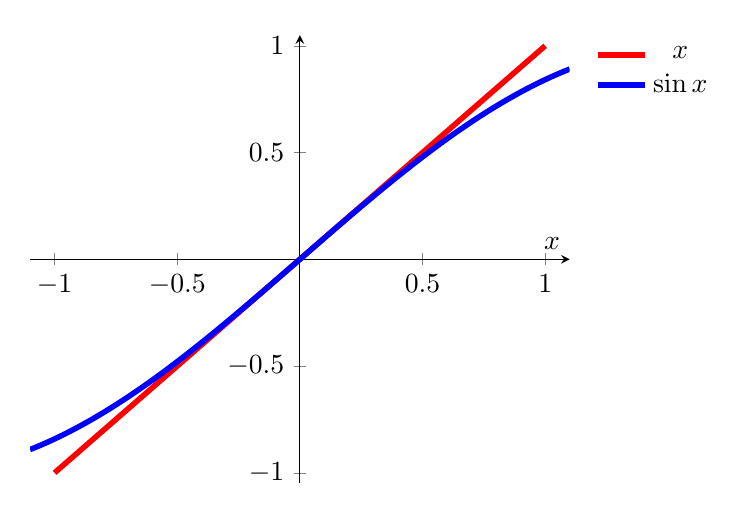
\begin{tikzpicture}
  \begin{axis}[
  axis x line=center, axis y line=center,
  ymax=1.05,ymin=-1.05, ytick={-1,-0.5,0.5,1.0},
  xtick={-1,-0.5,0.5,1},
  xlabel=$x$,
  legend entries={$x$,$\sin x$},
  legend pos=outer north east,
  legend style={draw=none}
  ]
  \addplot[line width=2pt, red,domain=-1:1,samples=100] {x};
  \addplot[line width=2pt, blue,domain=-1.1:1.1,samples=100] {sin(deg(x))};
  \end{axis}
\end{tikzpicture}
 \end{center}
\end{fig}
The above figure shows that the curves $y=x$ and $y=\sin x$ are almost the same
when $x$ is close to $0$. Hence if we want the value of
$\sin(1/10)$ we could just use this approximation $y=x$ to get
\begin{align*}
  \sin(1/10) \approx 1/10.
\end{align*}
Of course, in this case we simply observed that one function was a good
approximation of the other. We need to know how to find such approximations
more systematically.

More precisely, say we are given a function $f(x)$ that we wish to approximate
close to some point $x=a$, and we need to find another function $F(x)$
that
\begin{itemize}
 \item is simple and easy to compute\footnote{It is no good approximating a
function with something that is even more difficult to work with.}
 \item is a good approximation to $f(x)$ for $x$ values close to $a$.
\end{itemize}
Further, we would like to understand how good our approximation actually is.
Namely we need to be able to estimate the error $|f(x)-F(x)|$.

There are many different ways to approximate a function and we will discuss one
family of approximations: Taylor polynomials. This is an infinite family of
ever improving approximations, and our starting point is the very simplest.


%%%%%%%%%%%%%%%%%%%%%%%%%%%%%%%%%%%%%%%%%%%%%%%%%%%%%%%%%%%%%%%%%%%%%%
\subsection{Zeroth Approximation --- the Constant Approximation}\label{ssec const approx}
%%%%%%%%%%%%%%%%%%%%%%%%%%%%%%%%%%%%%%%%%%%%%%%%%%%%%%%%%%%%%%%%%%%%%%
The simplest functions are those that are constants. And our
zeroth\footnote{It barely counts as an approximation at all, but it will help
build intuition. Because of this, and the fact that a constant is a
polynomial of degree 0,  we'll start counting our approximations from zero
rather than 1.} approximation will be by a constant function. That is, the
approximating function will have the form $F(x)=A$, for some constant $A$.
Notice that this function is a polynomial of degree zero.


To ensure that $F(x)$ is a good approximation for $x$ close to $a$, we choose
$A$ so that $f(x)$ and $F(x)$ take exactly the same value when $x=a$.
\begin{align*}
F(x)=A\qquad\text{so}\qquad F(a)=A=f(a)\implies A=f(a)
\end{align*}
Our first, and crudest, approximation rule is
\begin{impeqn}[Constant approximation]\label{eq:constApprox}
\begin{align*}
f(x)\approx f(a)
\end{align*}
\end{impeqn}
\noindent An important point to note is that we need to know $f(a)$ --- if we cannot
compute that easily then we are not going to be able to proceed. We will often
have to choose $a$ (the point around which we are approximating $f(x)$) with
some care to ensure that we can compute $f(a)$.


Here is a figure showing the graphs of a typical $f(x)$ and approximating
function $F(x)$.
\vadjust{
    \begin{efig}
    \begin{center}
       \includegraphics{approx1}
    \end{center}
    \end{efig}
}
At $x=a$, $f(x)$ and $F(x)$ take the same value. For $x$ very near $a$,
the values of $f(x)$ and $F(x)$ remain close together. But the quality
of the approximation deteriorates fairly quickly as $x$ moves
away from $a$. Clearly we could do better with a straight line that follows the slope of
the curve. That is our next approximation.

But before then, an example:
\begin{eg}\label{eg ex const approx}
 Use the constant approximation to estimate $e^{0.1}$.

\soln First set $f(x) = e^x$.
\begin{itemize}
 \item Now we first need to pick a point $x=a$  to approximate the function. This point
needs to be close to $0.1$ and we need to be able to evaluate $f(a)$ easily. The obvious
choice is $a=0$.
\item Then our constant approximation is just
\begin{align*}
  F(x) &= f(0) = e^0 = 1\\
  F(0.1) &= 1
\end{align*}
\end{itemize}
Note that $e^{0.1} = 1.105170918\dots$, so even this approximation isn't too bad..
\end{eg}






%%%%%%%%%%%%%%%%%%%%%%%%%%%%%%%%%%%%%%%%%%%%%%%%%%%%%%%%%%%%%%%%%%%%%%
\subsection{First Approximation --- the Linear approximation}
%%%%%%%%%%%%%%%%%%%%%%%%%%%%%%%%%%%%%%%%%%%%%%%%%%%%%%%%%%%%%%%%%%%%%%
Our first\footnote{Recall that we started counting from
zero.} approximation improves on our zeroth approximation by allowing the approximating
function to be a linear function of $x$ rather than just a constant function. That is, we
allow $F(x)$ to be of the form $A+Bx$, for some constants $A$ and $B$.


To ensure that $F(x)$ is a good approximation for $x$ close to $a$, we still require that
$f(x)$ and $F(x)$ have the same value at $x=a$ (that was our zeroth approximation). Our
additional requirement is that their tangent lines at $x=a$ have the same slope --- that
the derivatives of $f(x)$ and $F(x)$ are the same at $x=a$. Hence
\begin{align*}
F(x)&=A+Bx  & &\implies & F(a)=A+Ba&=f(a)\\
F'(x)&=B    & &\implies & F'(a)=\phantom{A+a}B&=f'(a)
\end{align*}
So we must have $B=f'(a)$. Substituting this into $A+Ba=f(a)$ we get
$A=f(a)-af'(a)$. So
we can write
\begin{align*}
  F(x) &= A+Bx = \overbrace{f(a)- af'(a)}^A+ f'(a) \cdot x \\
  &= f(a) + f'(a) \cdot(x-a)
\end{align*}
We write it in this form because we can now clearly see that our first approximation is
just an extension of our zeroth approximation. This first approximation is also often
called the linear approximation of $f(x)$ about $x=a$.
\begin{impeqn}[Linear approximation]\label{eq:linApprox}
\begin{align*}
  f(x) \approx f(a)+f'(a)(x-a)
\end{align*}
\end{impeqn}
\noindent We should again stress that in order to form this approximation we need to know
$f(a)$ and $f'(a)$ --- if we cannot compute them easily then we are not going to be able
to proceed.



Recall, from Theorem \ref{thm:DIFFtangentLine}, that $y=f(a)+f'(a)(x-a)$
is exactly the equation of the tangent line to the curve $y=f(x)$ at $a$.
Here is a figure showing the graphs of a typical $f(x)$ and the approximating
function $F(x)$.
\vadjust{
    \begin{efig}
    \begin{center}
       \includegraphics{approx2}
    \end{center}
    \end{efig}
}
Observe that the graph of $f(a)+f'(a)(x-a)$ remains close to the
graph of $f(x)$ for a much larger range of $x$ than did the graph of our constant
approximation, $f(a)$. One can also see that we can improve this approximation if we can
use a function that curves down rather than being perfectly straight. That is our next
approximation.

But before then, back to our example:
\begin{eg}
 Use the linear approximation to estimate $e^{0.1}$.

\soln First set $f(x) = e^x$ and $a=0$ as before.
\begin{itemize}
 \item To form the linear approximation we need $f(a)$ and $f'(a)$:
\begin{align*}
  f(x) &= e^x & f(0) & = 1 \\
  f'(x) &= e^x & f'(0) & = 1
\end{align*}
\item Then our linear approximation is
\begin{align*}
  F(x) &= f(0) + x f'(0) = 1 + x \\
  F(0.1) &= 1.1
\end{align*}
\end{itemize}
Recall that $e^{0.1} = 1.105170918\dots$, so the linear approximation is
almost correct to 3 digits.
\end{eg}

It is worth doing another simple example here.
\begin{eg}
 Use a linear approximation to estimate $\sqrt{4.1}$.

\soln First set $f(x)=\sqrt{x}$. Hence $f'(x) = \frac{1}{2\sqrt{x}}$. Then we are trying
to approximate $f(4.1)$. Now we need to choose a sensible $a$ value.
\begin{itemize}
 \item We need to choose $a$ so that $f(a)$ and $f'(a)$ are easy to compute.
\begin{itemize}
 \item We could try $a=4.1$ --- but then we need to compute $f(4.1)$ and $f'(4.1)$ ---
which is our original problem and more!
\item We could try $a=0$ --- then $f(0)=0$ and $f'(0) = DNE$.
\item Setting $a=1$ gives us $f(1)=1$ and $f'(1)=\frac{1}{2}$. This would work, but we
can get a better approximation by choosing $a$ is closer to $4.1$.
\item Indeed we can set $a$ to be the square of any rational number and we'll get a
result that is easy to compute.
\item Setting $a=4$ gives $f(4)=2$ and $f'(4) = \frac{1}{4}$. This seems good enough.
\end{itemize}
\item Substitute this into equation~\eqref{eq:linApprox} to get
\begin{align*}
  f(4.1) &\approx f(4) + f'(4) \cdot(4.1-4) \\
  &= 2 + \frac{0.1}{4} = 2 + 0.025 = 2.025
\end{align*}
\end{itemize}
Notice that the true value is $\sqrt{4.1} = 2.024845673\dots$.
\end{eg}



%%%%%%%%%%%%%%%%%%%%%%%%%%%%%%%%%%%%%%%%%%%%%%%%%%%%%%%%%%%%%%%%%%%%%%
\subsection{Second Approximation --- the Quadratic Approximation}
%%%%%%%%%%%%%%%%%%%%%%%%%%%%%%%%%%%%%%%%%%%%%%%%%%%%%%%%%%%%%%%%%%%%%%

We next develop a still better approximation by now allowing the
approximating function be to a quadratic function of $x$. That is,
we allow $F(x)$ to be of the form $A+Bx+Cx^2$, for some constants $A$, $B$
and $C$. To ensure that $F(x)$ is a good approximation for $x$ close
to $a$, we choose $A$, $B$ and $C$ so that
\begin{itemize}
  \item $f(a)=F(a)$  (just as in our zeroth approximation),
  \item $f'(a)=F'(a)$ (just as in our first approximation), and
  \item $f''(a)=F''(a)$ --- this is a new condition.
\end{itemize}
These conditions give us the following equations
\begin{align*}
F(x)&=A+Bx+Cx^2  & &\implies & F(a)=A+Ba+\phantom{2}Ca^2&=f(a)\\
F'(x)&=B+2Cx & &\implies & F'(a)=\phantom{A+a}B+2Ca&=f'(a)\\
F''(x)&=2C   & &\implies & F''(a)=\phantom{A+aB+a}2C&=f''(a)
\end{align*}
Solve these for $C$ first, then $B$ and finally $A$.
\begin{align*}
C &=\half f''(a) & \text{substitute}\\
B &= f'(a) - 2Ca = f'(a)-af''(a) & \text{substitute again}\\
A &= f(a)-Ba-Ca^2 = f(a)-a[f'(a)-af''(a)]-\half f''(a)a^2
\end{align*}
Then put things back together to build up $F(x)$:
\begin{align*}
F(x)&=f(a)-f'(a)a+\half f''(a)a^2 & &\text{(this line is $A$)}\cr
&\phantom{=f(a)\hskip3pt}+f'(a)\,x\hskip3pt- f''(a)ax
   & & \text{(this line is $Bx$)}\\
&\phantom{=f(a)-f'(a)a\hskip3.5pt}+\half f''(a)x^2
 & &\text{(this line is $Cx^2$)}\\
&=f(a)+f'(a)(x-a)+\half f''(a)(x-a)^2
\end{align*}
Oof! We again write it in this form because we can now clearly see that our second
approximation is just an extension of our first approximation.

Our second approximation is called the quadratic approximation:
\begin{impeqn}[Quadratic approximation]\label{eq:quadApprox}
\begin{align*}
f(x)\approx f(a)+f'(a)(x-a)+\half f''(a)(x-a)^2
\end{align*}
\end{impeqn}
\noindent Here is a figure showing the graphs
of a typical $f(x)$ and approximating function $F(x)$.
\vadjust{
    \begin{efig}
    \begin{center}
       \includegraphics{approx3}
    \end{center}
    \end{efig}
}
This new approximation looks better than both the first and second.


Now there is actually an easier way to derive this approximation, which we show
you now. Let us rewrite\footnote{Any polynomial of degree two can be written in
this form. For example, when $a=1$, $3 + 2x + x^2 =   6 +  4(x-1) + (x-1)^2$.}
$F(x)$ so that it is easy to evaluate it and its derivatives at $x=a$:
\begin{align*}
  F(x) &= \alpha + \beta\cdot (x-a) + \gamma \cdot(x-a)^2
\end{align*}
Then
\begin{align*}
  F(x) &= \alpha + \beta\cdot (x-a) + \gamma \cdot(x-a)^2 &
  F(a) &= \alpha = f(a) \\
  F'(x) &= \beta + 2\gamma \cdot(x-a) &
  F'(a)&=\beta = f'(a) \\
  F''(x) &= 2\gamma &
  F''(a) &= 2\gamma = f''(a)
\end{align*}
And from these we can clearly read off the values of $\alpha,\beta$ and $\gamma$ and so
recover our function $F(x)$. Additionally if we write things this way, then it is quite
clear how to extend this to a cubic approximation and a quartic approximation and so
on.

Return to our example:
\begin{eg}
 Use the quadratic approximation to estimate $e^{0.1}$.

\soln Set $f(x) = e^x$ and $a=0$ as before.
\begin{itemize}
 \item To form the quadratic approximation we need $f(a), f'(a)$ and $f''(a)$:
\begin{align*}
  f(x) &= e^x & f(0) & = 1 \\
  f'(x) &= e^x & f'(0) & = 1\\
  f''(x) &= e^x & f''(0) & = 1
\end{align*}
\item Then our quadratic approximation is
\begin{align*}
  F(x) &= f(0) + x f'(0)  + \frac{1}{2} x^2 f''(0) = 1 + x + \frac{x^2}{2} \\
  F(0.1) &= 1.105
\end{align*}
\end{itemize}
Recall that $e^{0.1} = 1.105170918\dots$, so the quadratic approximation is quite
accurate with very little effort.
\end{eg}



Before we go on, let us first introduce (or revise) some notation that will make our
discussion easier.




%%%%%%%%%%%%%%%%%%%%%%%%%%%%%%%%%%%%%%%%%%%%%%%%%%%%%%%%%%%%%%%%%%%%%%

\subsection*{Whirlwind Tour of Summation Notation}
In the remainder of this section we will frequently need to write sums involving a
large number of terms. Writing out the summands explicitly can become quite
impractical --- for example, say we need the sum of the first 11 squares:
\begin{align*}
  1 + 2^2 + 3^2 + 4^2+ 5^2 + 6^2 + 7^2 + 8^2 + 9^2 + 10^2 + 11^2
\end{align*}
This becomes tedious. Where the pattern is clear, we will often skip the middle few
terms and instead write
\begin{align*}
  1 + 2^2 + \cdots  + 11^2.
\end{align*}
A far more precise way to write this is using $\Sigma$ (capital-sigma) notation. For
example, we can write the above sum as
\begin{align*}
  \sum_{k=1}^{11} k^2
\end{align*}
This is read as
\begin{quote}
 The sum from $k$ equals 1 to 11 of $k^2$.
\end{quote}
More generally
\begin{notn}
Let $m\leq n$ be integers and let $f(x)$ be a function defined on the integers.
Then we write
\begin{align*}
  \sum_{k=m}^n f(k)
\end{align*}
to mean the sum of $f(k)$ for $k$ from $m$ to $n$:
\begin{align*}
  f(m) + f(m+1) + f(m+2) + \cdots + f(n-1) + f(n).
\end{align*}
Similarly we write
\begin{align*}
  \sum_{i=m}^n a_i
\end{align*}
to mean
\begin{align*}
  a_m+a_{m+1}+a_{m+2}+\cdots+a_{n-1}+a_n
\end{align*}
for some set of coefficients $\{ a_m, \ldots, a_n \}$.
\end{notn}

Consider the example
\begin{align*}
\sum_{k=3}^7 \frac{1}{k^2}=\frac{1}{3^2}+\frac{1}{4^2}+\frac{1}{5^2}+
\frac{1}{6^2}+\frac{1}{7^2}
\end{align*}
It is important to note that the right hand side of this expression evaluates to a
number\footnote{Some careful addition shows it is $\frac{46181}{176400}$.}; it does not
contain ``$k$''.  The summation index $k$  is just a ``dummy'' variable and
it does not have to be called $k$. For example
\begin{align*}
  \sum_{k=3}^7 \frac{1}{k^2}
  =\sum_{i=3}^7 \frac{1}{i^2}
  =\sum_{j=3}^7 \frac{1}{j^2}
  =\sum_{\ell=3}^7 \frac{1}{\ell^2}
\end{align*}
Also the summation index has no meaning outside the sum. For
example
\begin{align*}
k\sum_{k=3}^7 \frac{1}{k^2}
\end{align*}
has no mathematical meaning; It is gibberish\footnote{Or possibly gobbledygook. For a
discussion of statements without meaning and why one should avoid them we recommend the
book ``Bendable learnings: the wisdom of modern management'' by Don Watson.}.



%%%%%%%%%%%%%%%%%%%%%%%%%%%%%%%%%%%%%%%%%%%%%%%%%%%%%%%%%%%%%%%%%%%%%%
\subsection{Still Better Approximations --- Taylor Polynomials}
%%%%%%%%%%%%%%%%%%%%%%%%%%%%%%%%%%%%%%%%%%%%%%%%%%%%%%%%%%%%%%%%%%%%%%
We can use the same strategy to generate still better approximations by
polynomials\footnote{Polynomials are generally a good choice for an approximating
function since they are so easy to work with. Depending on the situation other families
of functions may be more appropriate. For example if you are approximating a periodic
function, then sums of sines and cosines might be a better choice; this leads to Fourier
series.} of any degree we like. As was the case with the approximations above, we
determine the coefficients of the polynomial by requiring, that at the point
$x=a$, the approximation and its first $n$ derivatives agree with those of the
original function.

Rather than simply moving to a cubic polynomial, let us try to write things in a more
general way. We will consider approximating the function $f(x)$ using a polynomial,
$T_n(x)$, of degree $n$ --- where $n$ is a non-negative integer. As we discussed
above, the algebra is easier if we write
\begin{align*}
  T_n(x) &= c_0 + c_1(x-a) + c_2 (x-a)^2 + \cdots + c_n (x-a)^n\\
  &= \sum_{k=0}^n c_k (x-a)^k & \text{using $\Sigma$
notation}
\end{align*}
The above form\footnote{Any polynomial in $x$ of degree $n$ can also be
expressed as a polynomial in $(x-a)$ of the same degree $n$ and vice versa.  So
$T_n(x)$ really still is a polynomial of degree $n$.} \footnote{Furthermore
when $x$ is close to $a$, $(x-a)^k$ decreases very quickly as $k$ increases,
which often makes the "high $k$" terms in $T_n(x)$ very small. This can be a
considerable advantage when building up approximations by adding more and more
terms.  If we were to rewrite  $T_n(x)$ in the form $\ds \sum_{k=0}^n b_k x^k$
the "high $k$" terms would typically not be very small when $x$ is close to
$a$. } makes it very easy to evaluate this polynomial and its derivatives at
$x=a$. Before we proceed, we remind the reader of some notation (see
Notation~\ref{notn higher diff}):
\begin{itemize}
 \item Let $f(x)$ be a function and $k$ be a positive integer. We can denote
its $k^\mathrm{th}$ derivative with respect to $x$ by
\begin{align*}
  \ddiff{k}{f}{x} && \left( \diff{}{x}\right)^k f(x) && f^{(k)}(x)
\end{align*}
\end{itemize}

Additionally we will need
\begin{defn}[Factorial]
  Let $n$ be a positive integer\footnote{It is actually possible to define the
factorial of positive real numbers and even negative numbers but it requires more
advanced calculus and is outside the scope of this course. The interested reader should
look up the Gamma function.}, then $n$-factorial, denoted $n!$, is the product
  \begin{align*}
    n! &= n \times (n-1) \times \cdots \times 3 \times 2 \times 1
  \end{align*}
  Further, we use the convention that
  \begin{align*}
  0! &= 1
  \end{align*}
  The first few factorials are
\begin{align*}
  1! &=1 &
  2! &=2 &
  3! &=6 \\
  4! &=24 &
  5! &=120 &
  6! &=720
\end{align*}
\end{defn}

Now consider $T_n(x)$ and its derivatives:
\begin{align*}
\begin{array}{rclrrrcl}
  T_n(x) &=& c_0 &+ c_1(x-a) & + c_2 (x-a)^2 & + c_3(x-a)^3 &+ \cdots+ & c_n (x-a)^n
\\[1ex]
  T_n'(x) &=&  &c_1 & + 2 c_2 (x-a) & + 3c_3(x-a)^2 &+ \cdots +&  n c_n (x-a)^{n-1}
\\[1ex]
  T_n''(x) &=&  &  & 2 c_2 & + 6c_3(x-a) &+ \cdots +&  n(n-1) c_n (x-a)^{n-2} \\[1ex]
  T_n'''(x) &=&  &  & & 6c_3 &+ \cdots + &  n(n-1)(n-2) c_n (x-a)^{n-3} \\[1ex]
  & \vdots \\[1ex]
  T_n^{(n)}(x) &=&  &  & & & &  n! \cdot c_n
\end{array}
\end{align*}
Now notice that when we substitute $x=a$ into the above expressions only the constant
terms survive and we get
\begin{align*}
  T_n(a) &= c_0\\
  T_n'(a) &= c_1\\
  T_n''(a) &= 2\cdot c_2\\
  T_n'''(a) &= 6 \cdot c_3\\
  &\vdots \\
  T_n^{(n)}(a) &= n! \cdot c_n
\end{align*}
% We determine the coefficients $c_i$ by the requirements that $f(x)$ and
% its approximator $F(x)$ have the same value and the same first $n$
% derivatives at $x=a$.
% \begin{align*}
% F(x)&=c_0+c_1(x-a)+c_2(x-a)^2+\cdots+c_n(x-a)^n \hidewidth\\
%   &\hskip3.0in\implies  F(a)=c_0=f(a)\\
% F'(x)&=c_1+2c_2(x-a)+3c_3(x-a)^2+\cdots+nc_n(x-a)^{n-1} \hidewidth\\
%   &\hskip3.0in\implies   F'(a)=c_1=f'(a)    \displaybreak[0]\\
% F''(x)&=2c_2+3\times 2c_3(x-a)+\cdots+n(n-1)c_n(x-a)^{n-2}\hidewidth \\
%   &\hskip3.0in\implies  F''(a)=2c_2=f''(a)  \displaybreak[0]\\
% F^{(3)}(x)&=3\times 2 c_3+\cdots+n(n-1)(n-2)c_n(x-a)^{n-3} \hidewidth\\
%    &\hskip3.0in\implies F^{(3)}(a)=3\times 2c_3=f^{(3)}(a) \\
% &\hskip3.0in\ \ \ \,\vdots \\
% F^{(n)}(x)&=n! c_n
%    \hskip2,47in\implies F^{(n)}(a)= n! c_n=f^{(n)}(a)\\
% \end{align*}
% Here $n!=n(n-1)(n-2)\cdots 1$ is called $n$ factorial. Hence
% \begin{align*}
% c_0=f(a)\quad c_1=f'(a)\quad c_2=\tfrac{1}{2!}f''(a)
% \quad c_3=\tfrac{1}{3!}f^{(3)}(a)\quad\cdots\quad
%  c_n=\tfrac{1}{n!}f^{(n)}(a)
% \end{align*}
% and the approximator, which is called the Taylor polynomial of degree $n$
% for $f(x)$ at $x=a$, is
So now if we want to set the coefficients of $T_n(x)$ so that it agrees with
$f(x)$  at $x=a$ then we need
\begin{align*}
  T_n(a) &= c_0 = f(a) & c_0 &= f(a) = \frac{1}{0!} f(a)\\
\intertext{We also want the first $n$ derivatives of $T_n(x)$ to agree with the
derivatives of $f(x)$ at $x=a$, so}
  T_n'(a) &= c_1 = f'(a) & c_1 &= f'(a) = \frac{1}{1!} f'(a) \\
  T_n''(a) &= 2\cdot c_2 = f''(a) & c_2 &= \frac{1}{2} f''(a) = \frac{1}{2!}f''(a)\\
  T_n'''(a) &= 6\cdot c_3 = f'''(a) & c_3 &= \frac{1}{6} f'''(a) = \frac{1}{3!} f'''(a)
\intertext{More generally, making the $k^\mathrm{th}$ derivatives agree at $x=a$ requires
:}
  T_n^{(k)}(a) &= k!\cdot c_k = f^{(k)}(a) & c_k &= \frac{1}{k!} f^{(k)}(a)
\intertext{And finally the $n^\mathrm{th}$ derivative:}
  T_n^{(n)}(a) &= n!\cdot c_n = f^{(n)}(a) & c_n &= \frac{1}{n!} f^{(n)}(a)
\end{align*}
Putting this all together we have
\begin{impeqn}[Taylor polynomial]\label{eq:taylorPoly}
 \begin{align*}
  f(x) \approx T_n(x)
  &= f(a) + f'(a) (x-a) + \frac{1}{2} f''(a) \cdot(x-a)^2 + \cdots + \frac{1}{n!}
f^{(n)}(a) \cdot (x-a)^n \\
  &= \sum_{k=0}^n \frac{1}{k!} f^{(k)}(a) \cdot (x-a)^k
 \end{align*}
\end{impeqn}
Let us formalise this definition.
\begin{defn}[Taylor polynomial]
  Let $a$ be a constant and let $n$ be a non-negative integer. The $n^\mathrm{th}$
degree Taylor polynomial for $f(x)$ about $x=a$ is
\begin{align*}
  T_n(x) &= \sum_{k=0}^n \frac{1}{k!} f^{(k)}(a) \cdot (x-a)^k.
\end{align*}
  The special case $a=0$ is called a Maclaurin\footnote{The polynomials are named after
Brook Taylor who devised a general method for constructing them in 1715. Slightly
later, Colin Maclaurin made extensive use of the special case $a=0$ (with attribution of
the general case to Taylor) and it is now named after him. The special case of
$a=0$ was worked on previously by James Gregory and Isaac Newton, and some
specific cases were known to the 14th century Indian mathematician Madhava of
Sangamagrama.} polynomial.
\end{defn}

Before we proceed with some examples, a couple of remarks are in order.
\begin{itemize}
 \item While we can compute a Taylor polynomial about any $a$-value (providing the
derivatives exist), in order to be a \emph{useful} approximation, we must be able to
compute $f(a),f'(a),\dots,f^{(n)}(a)$ easily. This means we must choose the point $a$
with care. Indeed for many functions the choice $a=0$ is very natural --- hence the
prominence of Maclaurin polynomials.

\item If we have computed the approximation $T_n(x)$, then we can readily
extend this to the next Taylor polynomial $T_{n+1}(x)$ since
\begin{align*}
  T_{n+1}(x) &= T_n(x) + \frac{1}{(n+1)!} f^{(n+1)}(a) \cdot (x-a)^{n+1}
\end{align*}
This is very useful if we discover that $T_n(x)$ is an insufficient
approximation, because then we can produce $T_{n+1}(x)$ without having to start
again from scratch.
\end{itemize}

\subsection{Some Examples}
Let us return to our running example of $e^x$:
\begin{eg}\label{eg taylor e to the x}
 The constant, linear and quadratic approximations we used above were the first few
Maclaurin polynomial approximations of $e^x$. That is
\begin{align*}
  T_0 (x) & = 1 & T_1(x) &= 1+x & T_2(x) &= 1+x+\frac{x^2}{2}
\end{align*}
Since $\diff{}{x} e^x = e^x$, the Maclaurin polynomials are very easy to compute.
Indeed this invariance under differentiation means that
\begin{align*}
  f^{(n)}(x) &= e^x & n=0,1,2,\dots && \text{so}\\
  f^{(n)}(0) &= 1
\end{align*}
Substituting this into equation~\eqref{eq:taylorPoly} we get
\begin{align*}
  T_n(x) &= \sum_{k=0}^n \frac{1}{k!} x^k
\end{align*}
Thus we can write down the seventh Maclaurin polynomial very easily:
\begin{align*}
  T_7(x) &= 1 + x + \frac{x^2}{2} + \frac{x^3}{6} + \frac{x^4}{24} + \frac{x^5}{120} +
\frac{x^6}{720} + \frac{x^7}{5040}
\end{align*}
Also notice that if we use this to approximate the value of $e^1$ we obtain:
\begin{align*}
  e^1 \approx T_7(1) &= 1 + 1 + \frac{1}{2} + \frac{1}{6} + \frac{1}{24} + \frac{1}{120}
+ \frac{1}{720} + \frac{1}{5040} \\
  &= \frac{685}{252} =  2.718253968\dots
\end{align*}
The true value of $e$ is $2.718281828\dots$, so the approximation has an error of about
$3\times10^{-5}$.

Under the assumption that the accuracy of the approximation improves with
$n$ (an assumption we examine in Subsection~\ref{ssec taylor error} below) we can see
that the approximation of $e$ above can be improved by adding more and more terms. Indeed
this is how the expression for $e$ in equation~\eqref{eq:eulerconst} in
Section~\ref{sec exp func} comes about.
\end{eg}
Now that we have examined Maclaurin polynomials for $e^x$ we should take a look at $\log
x$. Notice that we cannot compute a Maclaurin polynomial for $\log x$ since it is not
defined at $x=0$.
\begin{eg}\label{eg expand logx}
Compute the $5^\mathrm{th}$ Taylor polynomial for $\log x$ about $x=1$.

\soln We have been told $a=1$ and fifth degree, so we should start by writing down the
function and its first five derivatives:
\begin{align*}
  f(x) &= \log x & f(1) &= \log 1 = 0 \\
  f'(x) &= \frac{1}{x} & f'(1) &= 1 \\
  f''(x) &= \frac{-1}{x^2} & f''(1) &= -1 \\
  f'''(x) &= \frac{2}{x^3} & f'''(1) &= 2 \\
  f^{(4)}(x) &= \frac{-6}{x^4} & f^{(4)}(1) &= -6 \\
  f^{(5)}(x) &= \frac{24}{x^5} & f^{(5)}(1) &= 24
\end{align*}
Substituting this into equation~\eqref{eq:taylorPoly} gives
\begin{align*}
  T_5(x)&= 0 + 1\cdot (x-1)
  + \frac{1}{2} \cdot (-1) \cdot (x-1)^2
  + \frac{1}{6} \cdot 2 \cdot (x-1)^3
  + \frac{1}{24} \cdot (-6) \cdot (x-1)^4
  + \frac{1}{120} \cdot 24 \cdot (x-1)^5 \\
  &= (x-1) - \frac{1}{2}(x-1)^2 + \frac{1}{3}(x-1)^3 - \frac{1}{4}(x-1)^4 +
\frac{1}{5}(x-1)^5
\end{align*}
Again, it is not too hard to generalise the above work to find the Taylor polynomial of
degree $n$:
With a little work one can show that
\begin{align*}
  T_n(x) &= \sum_{k=1}^n \frac{(-1)^{k+1}}{k} (x-1)^k.
\end{align*}
\end{eg}
For cosine:
\begin{eg}\label{eg expand cosx}
 Find the 4th degree Maclaurin polynomial for $\cos x$.

\soln We have $a=0$ and we need to find the first 4 derivatives of $\cos x$.
\begin{align*}
 f(x) &= \cos x & f(0) &= 1 \\
 f'(x) &= -\sin x & f'(0) &= 0 \\
 f''(x) &= -\cos x & f''(0) &= -1 \\
 f'''(x) &= \sin x & f'''(0) &= 0 \\
 f^{(4)}(x) &= \cos x & f^{(4)}(0) &= 1
\end{align*}
Substituting this into equation~\eqref{eq:taylorPoly} gives
\begin{align*}
  T_4(x)&= 1 + 1\cdot (0) \cdot x
  + \frac{1}{2} \cdot (-1) \cdot x^2
  + \frac{1}{6} \cdot 0 \cdot x^3
  + \frac{1}{24} \cdot (1) \cdot x^4 \\
  &= 1 - \frac{x^2}{2} + \frac{x^4}{24}
\end{align*}
Notice that since the $4^\mathrm{th}$ derivative of $\cos x$ is $\cos x$ again, we also
have that the fifth derivative is the same as the first derivative, and the sixth
derivative is the same as the second derivative and so on. Hence the next four
derivatives are
\begin{align*}
 f^{(4)}(x) &= \cos x & f^{(4)}(0) &= 1 \\
 f^{(5)}(x) &= -\sin x & f^{(5)}(0) &= 0 \\
 f^{(6)}(x) &= -\cos x & f^{(6)}(0) &= -1 \\
 f^{(7)}(x) &= \sin x & f^{(7)}(0) &= 0 \\
 f^{(8)}(x) &= \cos x & f^{(8)}(0) &= 1
\end{align*}
Using this we can find the $8^\mathrm{th}$ degree Maclaurin polynomial:
\begin{align*}
  T_8(x) &=
  1 - \frac{x^2}{2} + \frac{x^4}{24} -\frac{x^6}{6!} + \frac{x^8}{8!}
\end{align*}
Continuing this process gives us the $2n^\mathrm{th}$ Maclaurin polynomial
\begin{align*}
  T_{2n}(x) &= \sum_{k=0}^n \frac{(-1)^k}{(2k)!} \cdot x^{2k}
\end{align*}
\begin{warning}
The above formula only works when x is measured in radians, because all of our
derivative formulae for trig functions were developed under the assumption that
angles are measured in radians.
\end{warning}

Below we plot $\cos x$ against its first few Maclaurin polynomial
approximations:
\begin{efig}
\begin{center}

  \includegraphics{approx1d} \qquad\qquad
  \includegraphics{approx2d}
\end{center}
\begin{center}
  \includegraphics{approx3d} \qquad\qquad
  \includegraphics{approx4d}
\end{center}
\end{efig}

\end{eg}
The above work is quite easily recycled to get the Maclaurin polynomial for sine:
\begin{eg}\label{eg expand sinx}
 Find the 5th degree Maclaurin polynomial for $\sin x$.

\soln We could simply work as before and compute the first five derivatives of $\sin x$.
But set $g(x) = \sin x$ and notice that $g(x) = - f'(x)$, where $f(x) =\cos x$. Then we
have
\begin{align*}
  g(0) &= -f'(0) = 0 \\
  g'(0) &= -f''(0) = 1\\
  g''(0) &= -f'''(0) = 0\\
  g'''(0) &= -f^{(4)}(0) = -1\\
  g^{(4)}(0) &= -f^{(5)}(0) = 0\\
  g^{(5)}(0) &= -f^{(6)}(0) = 1
\end{align*}
Hence the required Maclaurin polynomial is
\begin{align*}
  T_5(x) &= x - \frac{x^3}{3!} + \frac{x^5}{5!}
\end{align*}
Just as we extended to the $2n^\mathrm{th}$ Maclaurin polynomial for cosine, we can also
extend our work to compute the $(2n+1)^\mathrm{th}$ Maclaurin polynomial for sine:
\begin{align*}
  T_{2n+1}(x) &= \sum_{k=0}^n \frac{(-1)^k}{(2k+1)!} \cdot x^{2k+1}
\end{align*}
\begin{warning}
The above formula only works when x is measured in radians, because all of our
derivative formulae for trig functions were developed under the assumption that
angles are measured in radians.
\end{warning}


Below we plot $\sin x$ against its first few Maclaurin polynomial approximations.
\begin{efig}
\begin{center}

  \includegraphics{approx1c} \qquad\qquad
  \includegraphics{approx2c}
\end{center}
\begin{center}
  \includegraphics{approx3c} \qquad\qquad
  \includegraphics{approx4c}
\end{center}
\end{efig}

\end{eg}

To get an idea of how good these Taylor polynomials are at approximating $\sin$ and
$\cos$, let's concentrate on $\sin x$ and consider $x$'s whose magnitude $|x|\le 1$.
There are tricks that you can employ\footnote{If you are writing software to evaluate
$\sin x$, you can always use the trig identity $\sin(x)=\sin(x-2n\pi)$, to  easily
restrict to $|x|\le\pi$. You can then use the trig identity $\sin(x)=-\sin(x\pm\pi)$ to
reduce to $|x|\le\tfrac{\pi}{2}$. Finally you can use the trig identity
$\sin(x)=\mp\cos(\tfrac{\pi}{2}\pm x))$ to reduce to $|x|\le\tfrac{\pi}{4} < 1$.} to
evaluate sine and cosine at values of $x$ outside this range.

If $|x|\le 1$ radians\footnote{Recall that the derivative formulae that we used to
derive the Taylor polynomials are valid only when $x$ is in radians. The
restriction $-1 \leq x \leq 1$ radians translates to angles bounded by
$\tfrac{180}{\pi}\approx 57^\circ$.}, then the magnitudes of the successive
terms in the Taylor polynomials for $\sin x$ are bounded by
\begin{align*}
|x|&\le 1 &
\tfrac{1}{3!}|x|^3&\le\tfrac{1}{6} &
\tfrac{1}{5!}|x|^5&\le\tfrac{1}{120}\approx 0.0083 \\
\tfrac{1}{7!}|x|^7&\le\tfrac{1}{7!}\approx 0.0002 &
\tfrac{1}{9!}|x|^9&\le\tfrac{1}{9!}\approx 0.000003 &
\tfrac{1}{11!}|x|^{11}&\le\tfrac{1}{11!}\approx 0.000000025
\end{align*}
From these inequalities, and the graphs on the previous pages, it certainly looks like,
for $x$ not too large, even relatively low degree Taylor polynomials give very good
approximations. In Section~\ref{ssec taylor error} we'll see how to get rigorous error
bounds on our Taylor polynomial approximations.




%%%%%%%%%%%%%%%%%%%%%%%%%%%%%%%%%%%%%%%%%%%%%%%%%%%%%%%%%%%%%%%%%%%%%%
\subsection{Estimating Change and $\De x$, $\De y$ Notation}
%%%%%%%%%%%%%%%%%%%%%%%%%%%%%%%%%%%%%%%%%%%%%%%%%%%%%%%%%%%%%%%%%%%%%%


Suppose that we have two variables $x$ and $y$ that are related by $y=f(x)$, for some
function $f$. One of the most important applications of calculus is to help us understand
what happens to $y$ when we make a small change in $x$.

\begin{notn}
 Let $x,y$ be variables related by a function $f$. That is $y = f(x)$. Then we denote a
  small change in the variable $x$ by $\De x$ (read as ``delta $x$''). The corresponding
small change in the variable $y$ is denoted $\De y$ (read as ``delta $y$'').
\begin{align*}
  \De y &= f(x+\De x) - f(x)
\end{align*}
\end{notn}

In many situations we do not need to compute $\De y$ exactly and are instead happy with
an approximation. Consider the following example.
\begin{eg}
Let $x$ be the number of cars manufactured per week in some factory and let $y$ the cost
of manufacturing those $x$ cars. Given that the factory currently produces $a$ cars per
week, we would like to estimate the increase in cost if we make a small change in the
number of cars produced.

\soln We are told that $a$ is the number of cars currently produced per week; the cost
of production  is then $f(a)$.
\begin{itemize}
 \item Say the number of cars produced is changed from $a$ to $a+\De x$ (where $\De x$
is some small number.
\item As $x$ undergoes this change, the costs change from $y=f(a)$ to $f(a+\De x)$.
Hence
\begin{align*}
  \De y &= f(a+\De x) - f(a)
\end{align*}
\item We can estimate this change using a linear approximation. Substituting
$x=a+\De x$ into the equation~\eqref{eq:linApprox} yields the approximation
\begin{align*}
f(a+\De x)\approx f(a)+f'(a)(a+\De x-a)
\end{align*}
and consequently the approximation
\begin{align*}
\De y=f(a+\De x)-f(a)\approx f(a)+f'(a)\De x-f(a)
\end{align*}
simplifies to the following neat estimate of $\De y$:
\begin{impeqn}[Linear approximation of $\De y$]\label{eq:lineDe}
\begin{align*}
    \De y\approx f'(a)\De x
\end{align*}
\end{impeqn}
\item In the automobile manufacturing example, when the production level is $a$ cars per
week, increasing the production level by $\De x$ will cost approximately
$f'(a)\De x$. The additional cost per additional car, $f'(a)$,  is called the ``marginal
cost'' of a car.

\item If we instead use the quadratic approximation (given by
equation~\eqref{eq:quadApprox}) then we estimate
\begin{align*}
f(a+\De x)\approx f(a)+f'(a)\De x+\half f''(a)\De x^2
\end{align*}
and so
\begin{align*}
\De y&=f(a+\De x)-f(a) \approx f(a)+f'(a)\De x +\half f''(a)\De x^2-f(a)
\end{align*}
which simplifies to
\begin{impeqn}[Quadratic approximation of $\De y$]\label{eq:quadDe}
\begin{align*}
  \De y &\approx f'(a)\De x+\half f''(a)\De x^2
\end{align*}
\end{impeqn}
\end{itemize}

\end{eg}

%%%%%%%%%%%%%%%%%%%%%%%%%%%%%%%%%%%%%%%%%%%%%%%%%%%%%%%%%%%%%%%%%%%%%%
\subsection{Further Examples}
%%%%%%%%%%%%%%%%%%%%%%%%%%%%%%%%%%%%%%%%%%%%%%%%%%%%%%%%%%%%%%%%%%%%%%
In this subsection we give further examples of computation and use of Taylor
approximations.

\begin{eg}\label{eg:taylorapprox}
Estimate $\tan 46^\circ$, using the constant-, linear- and quadratic-approximations
(equations~\eqref{eq:constApprox}, \eqref{eq:linApprox} and~\eqref{eq:quadApprox}).

\soln Note that we need to be careful to translate angles measured in degrees to radians.
\begin{itemize}
 \item Set $f(x)=\tan x$, $x=46\tfrac{\pi}{180}$ radians
and $a=45\tfrac{\pi}{180}=\tfrac{\pi}{4}$ radians.
This is a good choice for $a$ because
\begin{itemize}
\item  $a=45^\circ$ is close to $x=46^\circ$. As noted above, it is generally the case
that the closer $x$ is to $a$, the better various approximations will be.
\item We know the values of all trig functions at $45^\circ$.
\end{itemize}
\item Now we need to compute $f$ and its first two derivatives at $x=a$. It is a good
time to recall the special $1:1:\sqrt{2}$ triangle
\begin{efig}
 \begin{center}
  \includegraphics{triangle45}
 \end{center}
\end{efig}
So
\begin{align*}
  f(x) &= \tan x & f(\pi/4) &= 1\\
%
  f'(x) &= \sec^2 x = \frac{1}{\cos^2 x}
  & f'(\pi/4) &= \frac{1}{1/\sqrt{2}^2} = 2 \\
%
  f''(x) &=  \frac{2\sin x}{\cos^3 x}
  & f''(\pi/4) &= \frac{2/\sqrt{2}}{1/\sqrt{2}^3} = 4
\end{align*}
\item As $x-a=46\tfrac{\pi}{180}-45\tfrac{\pi}{180}=\tfrac{\pi}{180}$ radians, the
three approximations are
\begin{alignat*}{3}
f(x)&\approx f(a) &
    &&&=1\\
f(x)&\approx f(a)+f'(a)(x-a) &
    &=1+2\tfrac{\pi}{180} &
    &=1.034907\\
f(x)&\approx f(a)+f'(a)(x-a)+\half f''(a)(x-a)^2&
    &=1+2\tfrac{\pi}{180}+\half 4\big(\tfrac{\pi}{180}\big)^2 &
    & =1.035516
\end{alignat*}
For comparison purposes, $\tan 46^\circ$ really is $1.035530$ to 6 decimal
places.

\end{itemize}

\end{eg}

\begin{warning}\label{warning:radians}
All of our derivative formulae for trig functions were developed under
the assumption that angles are measured in radians.
Those derivatives appeared in the approximation formulae that we used
in Example \ref{eg:taylorapprox}, so we were obliged to express $x-a$
in radians.
\end{warning}


\begin{comment}
\begin{eg}\label{eg:taylorSinCos}
Let's find all Taylor polynomials for $\sin x$ and $\cos x$ at $x=a=0$.
To do so we merely need compute all derivatives of $\sin x$ and  $\cos x$
at $x=0$. First, compute all derivatives at general $x$.
\begin{equation}\label{eq:sinCosDerivs}
\begin{aligned}
f(x)&=\sin x &
f'(x)&=\cos x &
f''(x)&=-\sin x &
f^{(3)}(x)&=-\cos x &
f^{(4)}(x)&=\sin x & \cdots\\
g(x)&=\cos x &
g'(x)&=-\sin x &
g''(x)&=-\cos x &
g^{(3)}(x)&=\sin x &
g^{(4)}(x)&=\cos x & \cdots
\end{aligned}
\end{equation}
The pattern starts over again with the fourth derivative being the same
as the original function. Now set $x=a=0$.
\begin{equation}\label{eq:sinCosDerivsZero}
\begin{aligned}
f(x)&=\sin x &
f(0)&=0 &
f'(0)&=1 &
f''(0)&=0 &
f^{(3)}(0)&=-1 &
f^{(4)}(0)&=0 & \cdots\\
g(x)&=\cos x &
g(0)&=1 &
g'(0)&=0 &
g''(0)&=-1 &
g^{(3)}(0)&=0 &
g^{(4)}(0)&=1 & \cdots
\end{aligned}
\end{equation}
For $\sin x$, all even numbered derivatives are zero. The odd numbered
derivatives alternate between $1$ and $-1$.
For $\cos x$, all odd numbered derivatives are zero. The even numbered
derivatives alternate between $1$ and $-1$. So, the Taylor polynomials
that best approximate $\sin x$ and $\cos x$ near $x=a=0$ are
\begin{align*}
\sin x &\approx x-\tfrac{1}{3!}x^3+\tfrac{1}{5!}x^5-\cdots\\
\cos x &\approx 1-\tfrac{1}{2!}x^2+\tfrac{1}{4!}x^4-\cdots
\end{align*}
Here are graphs of $\sin x$ and its Taylor polynomials (about $x=a=0$)
up to degree seven.
\begin{efig}
\begin{center}

  \includegraphics{approx1c} \qquad\qquad
  \includegraphics{approx2c}
\end{center}
\begin{center}
  \includegraphics{approx3c} \qquad\qquad
  \includegraphics{approx4c}
\end{center}
\end{efig}
To get an idea of how good these Taylor polynomials are at
approximating $\sin$ and $\cos$, let's concentrate on $\sin x$ and consider
$x$'s whose magnitude $|x|\le 1$. (If you're writing software to evaluate
$\sin x$, you can always use the trig identity
$\sin(x)=\sin(x-2n\pi)$, to  easily restrict to $|x|\le\pi$, and then use
the trig identity $\sin(x)=-\sin(x\pm\pi)$ to reduce to $|x|\le\tfrac{\pi}{2}$
and then use the trig identity $\sin(x)=\mp\cos(\tfrac{\pi}{2}\pm x))$
to reduce to $|x|\le\tfrac{\pi}{4}$.) If $|x|\le 1$ radians (recall that
the derivative formulae that we used to derive the Taylor polynomials are
valid only when $x$ is in radians), or equivalently if $|x|$ is no larger
than $\tfrac{180}{\pi}\approx 57^\circ$, then the magnitudes of the successive
terms in the Taylor polynomials for $\sin x$ are bounded by
\begin{align*}
|x|&\le 1 &
\tfrac{1}{3!}|x|^3&\le\tfrac{1}{6} &
\tfrac{1}{5!}|x|^3&\le\tfrac{1}{120}\approx 0.0083 \\
\tfrac{1}{7!}|x|^7&\le\tfrac{1}{7!}\approx 0.0002 &
\tfrac{1}{9!}|x|^9&\le\tfrac{1}{9!}\approx 0.000003 &
\tfrac{1}{11!}|x|^{11}&\le\tfrac{1}{11!}\approx 0.000000025
\end{align*}
From these inequalities, and the graphs on the previous page, it
certainly looks like, for $x$ not too large, even relatively low degree
Taylor polynomials give very good approximations.
We'll see later how to get rigorous error bounds on our Taylor polynomial
approximations.
\end{eg}

\end{comment}

\begin{eg}\label{eg:taylorPole}
Suppose that you are ten meters from a vertical pole. You were
contracted to measure the height of the pole. You can't
take it down or climb it. So you measure the angle subtended by
the top of the pole. You measure $\theta=30^\circ$,  which gives
\begin{align*}
h=10\tan 30^\circ=\tfrac{10}{\sqrt{3}}\approx 5.77\text{m}\qquad\qquad
\end{align*}
This is just standard trigonometry ---  if we know the angle exactly then we know the
height exactly.

However, in the ``real world'' angles are hard to measure with such precision. If the
contract requires you the measurement of the pole to be accurate within $10$ cm, how
accurate does your measurement of the angle $\theta$ need to be?

\soln For simplicity\footnote{Mathematicians love assumptions that let us tame the real
world.}, we are going to assume that the pole is perfectly straight
and perfectly vertical and that your distance from the pole was exactly
10 m.
\begin{itemize}
\item Write $\theta=\theta_0+\De\theta$ where $\theta$ is the exact angle, $\theta_0$ is
the measured angle and $\De \theta$ is the error.
\item Similarly write $h=h_0+\De h$, where $h$ is the exact height and
$h_0=\tfrac{10}{\sqrt{3}}$ is the computed height. Their difference,
$\De h$, is the error.

\item Then
\begin{align*}
h_0&=10\tan\theta_0 & h_0+\De h&=10\tan(\theta_0+\De\theta)\\
\De h &= 10\tan(\theta_0+\De\theta) - 10\tan\theta_0
\end{align*}
We could attempt to solve this equation for $\De\theta$ in terms of $\De h$ --- but it is
far simpler to approximate $\De h$ using the linear approximation in
equation~\ref{eq:lineDe}.

\item To use equation~\ref{eq:lineDe}, replace $y$ with $h$, $x$ with $\theta$ and $a$
with $\theta_0$. Our function $f(\theta) = 10 \tan\theta$ and $\theta_0 = 30^\circ =
\pi/6$ radians. Then
\begin{align*}
  \De y &\approx f'(a) \De x & \text{ becomes }&&
  \De h &\approx f'(\theta_0) \De \theta
\end{align*}
Since $f(\theta)=10 \tan \theta$, $f'(\theta) = 10\sec^2\theta$ and
\begin{align*}
  f'(\theta_0) = 10\sec^2(\pi/6)
  = 10 \cdot \left(\frac{2}{\sqrt{3}} \right)^2 = \frac{40}{3}
\end{align*}

\item Putting things together gives
\begin{align*}
  \De h &\approx f'(\theta_0) \De \theta & \text{ becomes }&&
  \De h & \approx \frac{40}{3} \De \theta
\end{align*}
We can then solve this equation for $\De\theta$ in terms of $\De h$:
\begin{align*}
  \De \theta & \approx \frac{3}{40} \De h
\end{align*}

\item We are told that we must have $|\De h| < 0.1$, so we must have
\begin{align*}
  |\De \theta| &\leq \frac{3}{400}
\end{align*}
This is measured in radians, so converting back to degrees
\begin{align*}
  \frac{3}{400} \cdot \frac{180}{\pi} &= 0.43^\circ
\end{align*}

\end{itemize}

\end{eg}
\goodbreak

\begin{defn}\label{def:APPrelError} %%%%%%%%%%%%%%%%%%%%%
    Suppose that you measure, approximately, some quantity.
    Suppose that the exact value of that quantity is $Q_0$
    and that your measurement yielded $Q_0+\De Q$. Then
    $|\De Q|$ is called the absolute error of the measurement
    and $100\frac{|\De Q|}{Q_0}$ is called the percentage error
    of the measurement. As an example, if the exact
    value is $4$ and the measured value is $5$, then the absolute
    error is $|5-4|=1$ and the percentage error is
    $100\frac{|5-4|}{4}=25$. That is, the error, $1$, was $25\%$
    of the exact value, $4$.
\end{defn}


\begin{eg}\label{eg:taylorSphere}
Suppose that the radius of a sphere has been
measured with a percentage error of at most $\veps$\%. Find
the corresponding approximate percentage errors in the surface
area and volume of the sphere.

\soln We need to be careful in this problem to convert between absolute and percentage
errors correctly.

\begin{itemize}
\item Suppose that the exact radius is $r_0$ and that the measured radius is $r_0+\De r$.
\item Then the absolute error in the measurement is $|\De r|$ and, by definition, the
percentage error is $100\tfrac{|\De r|}{r_0}$. We are told that $100\tfrac{|\De
r|}{r_0}\le\veps$.

\item The surface area\footnote{We do not expect you to remember the surface areas of
solids for this course.} of a sphere of radius $r$ is $A(r)=4\pi r^2$. The error
in the surface area computed with the measured radius is
\begin{align*}
\De A &=A(r_0+\De r)-A(r_0)\approx A'(r_0)\De r\\
&= 8\pi r_0 \Delta r
\end{align*}
where we have made use of the linear approximation, equation~\eqref{eq:lineDe}.

\item The corresponding percentage error is then
\begin{align*}
100\frac{|\De A|}{A(r_0)}
\approx 100\frac{|A'(r_0)\De r|}{A(r_0)}
= 100\frac{8\pi r_0|\De r|}{4\pi r_0^2}
= 2\times 100\frac{|\De r|}{r_0}
\le 2\veps
\end{align*}


\item The volume of a sphere\footnote{We do expect you to remember the formula for the
volume of a sphere.} of radius $r$ is $V(r)=\frac{4}{3}\pi r^3$. The error in the volume
computed with the measured radius is
\begin{align*}
\De V &=V(r_0+\De r)-V(r_0)\approx V'(r_0)\De r \\
  &= 4\pi r_0^2 \Delta r
\end{align*}
where we have again made use of the linear approximation, equation~\eqref{eq:lineDe}.

\item The corresponding percentage error is
\begin{align*}
100\frac{|\De V|}{V(r_0)}
\approx 100\frac{|V'(r_0)\De r|}{V(r_0)}
= 100\frac{4\pi r_0^2|\De r|}{4\pi r_0^3/3}
= 3\times 100\frac{|\De r|}{r_0}
\le 3\veps
\end{align*}
\end{itemize}
We have just computed an approximation to $\Delta V$. This problem is actually
sufficiently simple that we can compute $\Delta V$ exactly:
\begin{align*}
  \Delta V &=  V(r_0 + \Delta r) - V(r_0)
	    = \tfrac{4}{3} \pi (r_0 + \Delta r)^3
	      - \tfrac{4}{3} \pi r_0^3
\end{align*}
\begin{itemize}
 \item Applying $(a+b)^3=a^3+3a^2b+3ab^2+b^3$ with $a=r_0$ and $b=\De r$, gives
\begin{align*}
V(r_0+\De r)-V(r_0)&=\tfrac{4}{3}\pi
\left[r_0^3+3r_0^2\De r+3r_0\,(\De r)^2+(\De r)^3\right] - \tfrac{4}{3}\pi  r_0^3\\
&=\tfrac{4}{3}\pi[3r_0^2\De r+3r_0\,(\De r)^2+(\De r)^3]
\end{align*}

\item Thus the difference between the exact error and the linear approximation
to the error is obtained by retaining only the last two terms in the square brackets. This
has magnitude
\begin{align*}
\tfrac{4}{3}\pi\big|3r_0\,(\De r)^2+(\De r)^3\big|
=\tfrac{4}{3}\pi\big|3r_0+\De r\big|(\De r)^2
\end{align*}
or in percentage terms
\begin{align*}
100\cdot \dfrac{1}{\tfrac{4}{3}\pi r_0^3} \cdot
\tfrac{4}{3}\pi \big|3r_0\,(\De r)^2+(\De r)^3\big|
%
&=100\left|3\frac{\De r^2}{r_0^2}+\frac{\De r^3}{r_0^3}\right|\\
%
&=\left(100 \frac{3\De r}{r_0}\right)
\cdot \left(\frac{\De r}{r_0}\right)
\left|1 +\frac{\De r}{3r_0}\right|\\
%
& \le 3\veps \left(\frac{\veps}{100}\right)\cdot \left(1+\frac{\veps}{300}\right)
\end{align*}
Since $\veps$ is small, we can assume that $1 + \frac{\veps}{300} \approx 1$. Hence the
difference between the exact error and the linear approximation of the error is roughly a
factor of $\tfrac{\veps}{100}$ smaller than the linear approximation $3\veps$.


\item As an aside, notice that if we argue that $\De r$ is very small and so we
can ignore terms involving $(\De r)^2$ and $(\De r)^3$ as being really really
small, then we obtain
\begin{align*}
V(r_0+\De r)-V(r_0)
&=\tfrac{4}{3}\pi[3r_0^2\De r \underbrace{+3r_0\,(\De r)^2+(\De
r)^3}_\text{really
really small}]\\
&\approx \tfrac{4}{3}\pi \cdot 3r_0^2\De r  = 4 \pi r_0^2 \De r
\end{align*}
which is precisely the result of our linear approximation above.


\end{itemize}
\end{eg}
\goodbreak

\begin{eg}\label{eg:taylorLamp}
To compute the height $h$ of a lamp post, the length $s$ of the
shadow of a two meter pole is measured. The pole is 6 m from the lamp post.
If the length of the shadow was measured to be 4 m, with an error of
at most one cm, find the height of the lamp post and estimate the
percentage error in the height.

\soln We should first draw a picture\footnote{We get to reuse that nice lamp post picture
from Example~\ref{eg:fallingBall}.}
\begin{efig}
 \begin{center}
  \includegraphics[height=6cm]{extra/lamp_shadow}
 \end{center}
\end{efig}
\begin{itemize}
\item By similar triangles we see that
\begin{align*}
    \frac{2}{s} &= \frac{h}{6+s}
\end{align*}
from which we can isolate $h$ as a function of $s$:
\begin{align*}
  h &= \frac{2(6+s)}{s} = \frac{12}{s} + 2
\end{align*}
\item The length of the shadow was measured to be $s_0=4$ m. The corresponding
height of the lamp post is
\begin{align*}
  h_0 &= \frac{12}{4} + 2 = 5m
\end{align*}

\item If the error in the measurement of the length of the shadow was $\De s$, then the
exact shadow length was $s=s_0+\De s$ and the exact lamp post height is $h=f(s_0+\De s)$,
where $f(s)=\tfrac{12}{s}+2$. The error in the computed lamp post height is
\begin{align*}
  \De h=h-h_0=f(s_0+\De s)-f(s_0)
\end{align*}

\item We can then make a linear approximation of this error using
equation~\eqref{eq:lineDe}:
\begin{align*}
\De h &\approx f'(s_0)\De s =-\frac{12}{s_0^2}\De s =-\frac{12}{4^2}\De s
\end{align*}
\item We are told that $|\De s|\le\frac{1}{100}$ m. Consequently, approximately,
\begin{align*}
 |\De h|\le \frac{12}{4^2}\frac{1}{100}=\frac{3}{400}
\end{align*}
The percentage error is then approximately
\begin{align*}
  100\frac{|\De h|}{h_0} & \le 100\frac{3}{400\times 5}=0.15\%
\end{align*}
\end{itemize}
\end{eg}

% \begin{eg}\label{eg:taylorPlane}
% \issue{Joel:\\ Replace\\ this?}
% When an aircraft crosses the Atlantic ocean at a speed of $u$ mph, the
% flight costs the company
% \begin{align*}
% C(u)=100+\tfrac{u}{3}+\tfrac{240,000}{u}
% \end{align*}
% dollars per passenger.
% When there is no wind, the aircraft flies at an airspeed of $550$mph.
% Find the approximate savings, per passenger, when there is a
% $35$ mph tail wind and estimate the cost when there is a $50$ mph head wind.
%
% \soln
% Let $u_0=550$. When the aircraft flies at speed $u_0$, the cost per passenger
% is $C(u_0)$. By \eqref{eq:lineDe}, a change of $\De u$ in the airspeed
% results in an change of
% \begin{align*}
% \De C\approx C'(u_0)\De u
% =\big[\tfrac{1}{3}-\tfrac{240,000}{u_0^2}\big]\De u
% =\big[\tfrac{1}{3}-\tfrac{240,000}{550^2}\big]\De u
% \approx-.460\De u
% \end{align*}
% in the cost per passenger. With the tail wind $\De u=35$ and the resulting
% \begin{align*}
% \De C\approx -.460\times 35=-16.10
% \end{align*}
% so there is a savings of $\$16.10$. With the head wind $\De u=-50$ and
% the resulting
% \begin{align*}
% \De C\approx -.4601\times (-50)=23.01
% \end{align*}
% so there is an additional cost of about $\$23.00$.
% \end{eg}
%

\goodbreak



%%%%%%%%%%%%%
\subsection{The Error in the Taylor Polynomial Approximations}\label{ssec taylor error}
%%%%%%%%%%%%%%
Any time you make an approximation, it is desirable to have some idea
of the size of the error you introduced. That is, we would like to know the difference
$R(x)$ between the original function $f(x)$ and our approximation $F(x)$:
\begin{align*}
  R(x) &= f(x)-F(x).
\end{align*}
Of course if we know $R(x)$ exactly, then we could recover $f(x) = F(x)+R(x)$ --- so this
is an unrealistic hope. In practice we would simply like to bound $R(x)$:
\begin{align*}
  |R(x)| &= |f(x)-F(x)| \leq M
\end{align*}
where (hopefully) $M$ is some small number. It is worth stressing that we do not need the
tightest possible value of $M$, we just need a relatively easily computed $M$ that isn't
too far off the true value of $|f(x)-F(x)|$.


We will now develop a formula for the error introduced by the constant approximation,
equation~\eqref{eq:constApprox} (developed back in Section~\ref{ssec const
approx})
\begin{align*}
f(x)&\approx f(a) = T_0(x) & \text{$0^\mathrm{th}$ Taylor polynomial}
\end{align*}
The resulting formula can be used to get an upper bound on the size of the error
$|R(x)|$.

The main ingredient we will need is the Mean-Value Theorem (Theorem~\ref{thm:DIFFmvt})
--- so we suggest you quickly revise it. Consider the following obvious statement:
\begin{align*}
  f(x) &= f(x) & \text{now some sneaky manipulations}\\
  & = f(a) + (f(x)-f(a)) \\
  &= \underbrace{f(a)}_{=T_0(x)} + (f(x)-f(a)) \cdot \underbrace{\frac{x-a}{x-a}}_{=1} \\
  &= T_0(x) + \underbrace{\frac{f(x)-f(a)}{x-a}}_\text{looks familiar} \cdot (x-a)
\end{align*}
Indeed, this equation is important in the discussion that follows, so we'll highlight it
\begin{impeqn}[We will need it again soon]\label{eq:taylorErrorA}
 \begin{align*}
  f(x) &= T_0(x) + \left[ \frac{f(x)-f(a)}{x-a} \right](x-a)
 \end{align*}
\end{impeqn}
The coefficient $\dfrac{f(x)-f(a)}{x-a}$ of $(x-a)$ is the average slope
of $f(t)$ as $t$ moves from $t=a$ to $t=x$. We can picture this as the slope of the
secant joining the points $(a,f(a))$ and $(x,f(x))$ in the sketch below.
\vadjust{
  \begin{efig}
  \begin{center}
     \includegraphics{approx4bb}
  \end{center}
  \end{efig}
}

As $t$ moves from $a$ to $x$, the instantaneous slope $f'(t)$ keeps changing. Sometimes
$f'(t)$ might be larger than the average slope $\tfrac{f(x)-f(a)}{x-a}$, and sometimes
$f'(t)$ might be smaller than the average slope $\tfrac{f(x)-f(a)}{x-a}$. However, by the
Mean-Value Theorem (Theorem~\ref{thm:DIFFmvt}), there must be some number $c$, strictly
between $a$ and $x$, for which  $f'(c)=\dfrac{f(x)-f(a)}{x-a}$ exactly.


Substituting this into formula \eqref{eq:taylorErrorA} gives
\begin{impeqn}[Towards the error]\label{eq:taylorErrorL}
\begin{align*}
  f(x) &=T_0(x) +f'(c)(x-a) & \text{for some $c$ strictly between $a$ and $x$}
\end{align*}
\end{impeqn}
Notice that this expression as it stands is not quite what we want. Let us massage this
around a little more into a more useful form
\begin{impeqn}[The error in constant approximation]\label{eq:taylorErrorL2}
 \begin{align*}
  f(x) - T_0(x) &= f'(c) \cdot (x-a) & \text{for some $c$ strictly between
$a$ and $x$}
\end{align*}
\end{impeqn}
Notice that the MVT doesn't tell us the value of $c$, however we do know that it lies
strictly between $x$ and $a$. So if we can get a good bound on $f'(c)$ on this interval
then we can get a good bound on the error.

\begin{eg}\label{eg zero approx of e}
  Let us return to Example~\ref{eg ex const approx}, and we'll try to bound the error in
our approximation of~$e^{0.1}$.

\begin{itemize}
 \item Recall that $f(x) = e^x$, $a=0$ and $T_0(x) = e^0 = 1$.
 \item Then by equation~\eqref{eq:taylorErrorL2}
  \begin{align*}
    e^{0.1} - T_0(0.1) &= f'(c) \cdot (0.1 - 0) & \text{with $0<c<0.1$}
  \end{align*}
  \item Now $f'(c) = e^c$, so we need to bound $e^c$ on $(0,0.1)$. Since $e^c$ is an
  increasing function, we know that
  \begin{align*}
    e^0 &< f'(c) < e^{0.1}  & \text{ when $0<c<0.1$}
  \end{align*}
  So one is tempted to write that
  \begin{align*}
    |e^{0.1} - T_0(0.1)| &= |R(x)| = |f'(c)| \cdot (0.1 - 0)\\
    & < e^{0.1} \cdot 0.1
  \end{align*}
  And while this is true, it is rather circular. We have just bounded the error in our
  approximation of $e^{0.1}$ by $\frac{1}{10}e^{0.1}$ --- if we actually knew $e^{0.1}$
  then we wouldn't need to estimate it!

  \item While we don't know $e^{0.1}$ exactly, we do know\footnote{Oops! Do we
really know that $e<3$? We haven't proved it. We will do so soon.}
that $1 = e^0 < e^{0.1} < e^1 <
3$. This   gives us
  \begin{align*}
    |R(0.1)| < 3 \times 0.1 = 0.3
  \end{align*}
  That is --- the error in our approximation of $e^{0.1}$ is no greater than $0.3$.
  Recall that we don't need the error exactly, we just need a good idea of how large it
  actually is.

  \item In fact the real error here is
\begin{align*}
  |e^{0.1} - T_0(0.1)| &=|e^{0.1} - 1| = 0.1051709\dots
\end{align*}
so we have over-estimated the error by a factor of 3.
\end{itemize}

But we can actually go a little further here --- we can bound the error above and below.
If we do not take absolute values, then since
  \begin{align*}
    e^{0.1} - T_0(0.1) &= f'(c) \cdot 0.1 & \text{ and } 1 < f'(c) < 3
  \end{align*}
we can write
\begin{align*}
  1\times 0.1 \leq ( e^{0.1} - T_0(0.1) ) & \leq 3\times 0.1
\end{align*}
so
\begin{align*}
  T_0(0.1) + 0.1 &\leq e^{0.1} \leq T_0(0.1)+0.3 \\
  1.1 &\leq e^{0.1} \leq 1.3
\end{align*}
So while the upper bound is weak, the lower bound is quite tight.

\end{eg}

There are formulae similar to equation~\eqref{eq:taylorErrorL}, that can be used to bound
the error in our other approximations; all are based on generalisations of the
MVT. The
next one --- for linear approximations --- is
\begin{align*}
f(x) & =\underbrace{f(a)+f'(a)(x-a)}_{=T_1(x)}+\half f''(c)(x-a)^2 &
\text{for some $c$ strictly between $a$ and $x$}
\end{align*}
which we can rewrite in terms of $T_1(x)$:
\begin{impeqn}[The error in linear approximation]\label{eq:taylorErrorQ}
\begin{align*}
f(x)-T_1(x) &=  \half f''(c)(x-a)^2 & \text{for some $c$ strictly between $a$ and $x$}
\end{align*}
\end{impeqn}
It implies that the error that we make when we approximate $f(x)$ by
$T_1(x) = f(a)+f'(a)\,(x-a)$ is exactly $\half f''(c)\,(x-a)^2$ for some $c$ strictly
between $a$ and $x$.


More generally
\begin{align*}
f(x)=&
\underbrace{f(a)+f'(a)\cdot(x-a)+\cdots+\frac{1}{n!}f^{(n)}(a)\cdot(x-a)^n}_{= T_n(x)}
+\frac{1}{(n+1)!}f^{(n+1)}(c)\cdot (x-a)^{n+1}
\end{align*}
for some $c$ strictly between $a$ and $x$. Again, rewriting this in terms of $T_n(x)$
gives
\begin{impeqn}\label{eq:taylorErrorN}
\begin{align*}
  f(x) - T_n(x) &= \frac{1}{(n+1)!}f^{(n+1)}(c)\cdot (x-a)^{n+1}
& \text{for some $c$ strictly between $a$ and $x$}
\end{align*}
\end{impeqn}

That is, the error introduced when $f(x)$ is approximated by its Taylor
polynomial of degree $n$, is precisely the last term of the Taylor polynomial
of degree $n+1$, but with the derivative evaluated at some point between
$a$ and $x$, rather than exactly at $a$. These error formulae are proven
in the optional Section~\ref{subsec:GMVT} later in this chapter.


\begin{eg}\label{eg:taylorErrorSin}
Approximate $\sin 46^\circ$ using Taylor polynomials about
$a=45^\circ$, and estimate the resulting error.

\soln
\begin{itemize}
 \item Start by defining $f(x) = \sin x$ and
\begin{align*}
a&=45^\circ=45\tfrac{\pi}{180} {\rm radians}&
x&=46^\circ=46\tfrac{\pi}{180} {\rm radians}&
x-a&=\tfrac{\pi}{180} {\rm radians}
\end{align*}
\item The first few derivatives of $f$ at $a$ are
\begin{alignat*}{2}
f(x)&=\sin x
&f(a)&=\frac{1}{\sqrt{2}}\\
f'(x)&=\cos x &
f'(a)&=\frac{1}{\sqrt{2}}\\
f''(x)&=-\sin x &
f''(a)&=-\frac{1}{\sqrt{2}}\\
f^{(3)}(x)&=-\cos x &
f^{(3)}(a)&=-\frac{1}{\sqrt{2}}
\end{alignat*}
\item
The constant, linear and quadratic Taylor approximations for $\sin(x)$ about
$\frac{\pi}{4}$ are
\begin{alignat*}{4}
  T_0(x) &= f(a)
    &&= \frac{1}{\sqrt{2}} \\
  T_1(x) &= T_0(x) + f'(a) \cdot(x-a)
    &&= \frac{1}{\sqrt{2}} + \frac{1}{\sqrt{2}}\left(x - \frac{\pi}{4} \right)\\
  T_2(x) &= T_1(x) + \half f''(a) \cdot(x-a)^2
    &&=  \frac{1}{\sqrt{2}} + \frac{1}{\sqrt{2}}\left(x - \frac{\pi}{4} \right)
  - \frac{1}{2\sqrt{2}}\left(x - \frac{\pi}{4} \right)^2
\end{alignat*}
\item So the approximations for $\sin 46^\circ$ are
\begin{align*}
\sin46^\circ &\approx T_0\left(\frac{46\pi}{180}\right) = \frac{1}{\sqrt{2}} &
=0.70710678\\
%%
\sin46^\circ &\approx T_1\left(\frac{46\pi}{180}\right)
= \frac{1}{\sqrt{2}} + \frac{1}{\sqrt{2}} \left(\frac{\pi}{180}\right)
&=0.71944812\\
%%
\sin46^\circ&\approx T_2\left(\frac{46\pi}{180}\right)
= \frac{1}{\sqrt{2}} + \frac{1}{\sqrt{2}} \left(\frac{\pi}{180}\right)
- \frac{1}{2\sqrt{2}}\left(\frac{\pi}{180}\right)^2
 &=0.71934042
\end{align*}
\item The errors in those approximations are (respectively)
\begin{alignat*}{3}
&{\rm error\ in\ 0.70710678}&
     &=f'(c)(x-a)&
     &=\cos c \cdot \left(\frac{\pi}{180}\right)\\
%
&{\rm error\ in\ 0.71944812}&
   &=\frac{1}{2} f''(c)(x-a)^2&
   &=-\frac{1}{2} \cdot \sin c\cdot \left(\frac{\pi}{180}\right)^2\\
&{\rm error\ in\ 0.71923272}&
   &=\frac{1}{3!}f^{(3)}(c)(x-a)^3&
   &=-\frac{1}{3!}\cdot \cos c \cdot \left(\frac{\pi}{180}\right)^3
\end{alignat*}
In each of these three cases $c$ must lie somewhere between $45^\circ$ and
$46^\circ$.

\item Rather than carefully estimating $\sin c$ and $\cos c$ for $c$ in that range, we
make use of a simpler (but much easier bound). No matter what $c$ is, we know that $|\sin
c|\le 1$ and $|\cos c|\le 1$. Hence
\begin{alignat*}{3}
&\big|{\rm error\ in\ 0.70710678}\big|&
   &\le  \left(\frac{\pi}{180}\right)&
   &<0.018\\
&\big|{\rm error\ in\ 0.71944812}\big|&
   &\le\frac{1}{2} \left(\frac{\pi}{180}\right)^2&
   &<0.00015\\
&\big|{\rm error\ in\ 0.71934042}\big|&
   &\le \frac{1}{3!} \left(\frac{\pi}{180}\right)^3&
  &<0.0000009
\end{alignat*}
\end{itemize}

\end{eg}
\begin{eg}[Showing $e<3$]
In Example~\ref{eg zero approx of e} above we used the fact that $e<3$ without actually
proving it. Let's do so now.

\begin{itemize}
 \item Consider the linear approximation of $e^x$ about $a=0$.
\begin{align*}
  T_1(x) &= f(0) + f'(0)\cdot x = 1 + x
\end{align*}
So at $x=1$ we have
\begin{align*}
  e &\approx T_1(1) = 2
\end{align*}

\item The error in this approximation is
\begin{align*}
  e^x - T_1(x) &= \frac{1}{2} f''(c) \cdot x^2 = \frac{e^c}{2} \cdot x^2
\end{align*}
So at $x=1$ we have
\begin{align*}
  e - T_1(1) &= \frac{e^c}{2}
\end{align*}
where $0<c<1$.

\item Now since $e^x$ is an increasing\footnote{Since the derivative of $e^x$ is $e^x$
which is positive everywhere, the function is increasing everywhere.} function, it
follows that $e^c < e$. Hence
\begin{align*}
  e - T_1(1) &= \frac{e^c}{2} < \frac{e}{2}
\end{align*}
Moving the $\frac{e}{2}$ to the left hand side and the $T_1(1)$ to the right
hand side gives
\begin{align*}
  \frac{e}{2} \leq T_1(1) = 2
\end{align*}
So $e<4$.

\item This isn't as tight as we would like --- so now do the same with the
quadratic approximation with $a=0$:
\begin{align*}
  e^x & \approx T_2(x) = 1 + x + \frac{x^2}{2}
\intertext{So when $x=1$ we have}
  e & \approx T_2(1) = 1 + 1 + \frac{1}{2} = \frac{5}{2}
\end{align*}
\item The error in this approximation is
\begin{align*}
  e^x - T_2(x) &= \frac{1}{3!} f'''(c) \cdot x^3 = \frac{e^c}{6} \cdot x^3
\end{align*}
So at $x=1$ we have
\begin{align*}
  e - T_2(1) &= \frac{e^c}{6}
\end{align*}
where $0<c<1$.

\item Again since $e^x$ is an increasing function we have $e^c < e$. Hence
\begin{align*}
  e - T_2(1) &= \frac{e^c}{6} < \frac{e}{6}
\end{align*}
That is
\begin{align*}
  \frac{5e}{6} < T_2(1) = \frac{5}{2}
\end{align*}
So $e<3$ as required.

\end{itemize}

\end{eg}



\begin{eg}[More on $e^x$]\label{eg:exp}
We wrote down the general $n^\mathrm{th}$ degree Maclaurin polynomial approximation of
$e^x$ in Example~\ref{eg taylor e to the x} above.
\begin{itemize}
 \item Recall that
\begin{align*}
  T_n(x) &= \sum_{k=0}^n \frac{1}{k!} x^k
\end{align*}
\item The error in this approximation is (by equation~\eqref{eq:taylorErrorN})
\begin{align*}
  e^x - T_n(x) &= \frac{1}{(n+1)!} e^c
\end{align*}
where $c$ is some number between $0$ and $x$.

\item So setting $x=1$ in this gives
\begin{align*}
  e - T_n(1) &= \frac{1}{(n+1)!} e^c
\end{align*}
where $0<c<1$.
\item Since $e^x$ is an increasing function we know that $1 = e^0 < e^c < e^1 < 3$, so
the above expression becomes
\begin{align*}
  \frac{1}{(n+1)!} \leq e - T_n(1) &= \frac{1}{(n+1)!} e^c \leq \frac{3}{(n+1)!}
\end{align*}
\item So when $n=9$ we have
\begin{align*}
  \frac{1}{10!} \leq e - \left(1 + 1 + \frac{1}{2} +\cdots + \frac{1}{9!} \right) &\leq
  \frac{3}{10!}
\end{align*}
\item Now $1/10! < 3/10! < 10^{-6}$, so the approximation of $e$ by
\begin{align*}
  e \approx 1 + 1 + \frac{1}{2} +\cdots + \frac{1}{9!} = \frac{98641}{36288} =
2.718281\dots
\end{align*}
is correct to 6 decimal places.

\item More generally we know that using $T_n(1)$ to approximate $e$ will have an error of
at most $\frac{3}{(n+1)!}$ --- so it converges very quickly.
\end{itemize}

% Let $f(x)=e^x$. Then
% \begin{align*}
% f(x)&=e^x & &\Rightarrow &
% f'(x)&=e^x & &\Rightarrow &
% f''(x)&=e^x & &\cdots \\
% f(0)&=e^0=1 & &\Rightarrow &
% f'(0)&=e^0=1 & &\Rightarrow &
% f''(0)&=e^0=1 & &\cdots
% \end{align*}
% Applying \eqref{eq:taylorErrorN} with $f(x)=e^x$ and $a=0$,
% and using that $f^{(m)}(a)=e^{a}=e^0=1$ for all $m$,
% \begin{equation}\label{eq:expTaylor}
% e^x=f(x)=
% 1+x+\tfrac{x^2}{2!}+\cdots+\tfrac{x^n}{n!}+\tfrac{1}{(n+1)!}e^c x^{n+1}
% \end{equation}
% for some $c$ between $0$ and $x$. We can use this to find approximate values
% for the number $e$, with any desired degree of accuracy. Just setting $x=1$ in
% \eqref{eq:expTaylor} gives
% \begin{equation}\label{eq:eTaylor}
% e=1+1+\tfrac{1}{2!}+\cdots+\tfrac{1}{n!}+\tfrac{1}{(n+1)!}e^c
% \end{equation}
% for some $c$ between $0$ and $1$. Since $e^c$ increases as $c$ increases,
% this says that $1+1+\tfrac{1}{2!}+\cdots+\tfrac{1}{n!}$ is an approximate
% value for $e$ with error at most $\tfrac{e}{(n+1)!}$. The only problem
% with this error bound is that it contains the number $e$, which we do not
% know. Fortunately, we can again use \eqref{eq:eTaylor} to get a simple
% upper bound on how big $e$ can be. Just setting $n=2$ in \eqref{eq:eTaylor},
% and again using that $e^c\le e$, gives
% \begin{align*}
% e\le 1+1+\tfrac{1}{2!}+\tfrac{e}{3!}
% \implies
% \big(1-\tfrac{1}{6}\big)e\le  1+1+\tfrac{1}{2!}=\tfrac{5}{2}
% \implies
% e\le \tfrac{5}{2}\times\tfrac{6}{5}=3
% \end{align*}
% So we now know that $1+1+\tfrac{1}{2!}+\cdots+\tfrac{1}{n!}$ is an approximate
% value for $e$ with error at most $\tfrac{3}{(n+1)!}$. For example,
% when $n=9$, $\tfrac{3}{(n+1)!}=\tfrac{3}{10!}<10^{-6}$ so that
% \begin{align*}
% 1+1+\tfrac{1}{2!}+\cdots+\tfrac{1}{9!}
% \le e\le
% 1+1+\tfrac{1}{2!}+\cdots+\tfrac{1}{9!} +10^{-6}
% \end{align*}
% with
% \begin{alignat*}{10}
% &1+1 &
%   &+\ \tfrac{1}{2!} &
%   &+\ \ \tfrac{1}{3!}\ &
%   &+\hskip10pt\tfrac{1}{4!}\hskip10pt &
%   &+\hskip10pt\tfrac{1}{5!}\hskip10pt &
%   &+\hskip10pt\tfrac{1}{6!}\hskip10pt &
%   &+\hskip15pt\tfrac{1}{7!}\hskip15pt &
%   &+\hskip15pt\tfrac{1}{8!}\hskip15pt &
%   &+\hskip15pt\tfrac{1}{9!}
% \\
%  =&1+1&
%  &+0.5&
%  &+0.1\dot 6&
%  &+0.041\dot 6&
%  &+0.008\dot 3&
%  &+0.0013\dot 8&
%  &+0.0001984&
%  &+0.0000248&
%  &+0.0000028\\
% =&2.718282\hidewidth
% \end{alignat*}
% to six decimal places.

\end{eg}

\begin{eg}[Example \ref{eg:taylorPole} Revisited]
Recall\footnote{Now is a good time to go back and re-read it.} that in Example
\ref{eg:taylorPole} (measuring the height of the pole), we
used the linear approximation
\begin{align*}%\label{eq:taylorErrorPole}
f(\theta_0+\De\theta)&\approx f(\theta_0)+f'(\theta_0)\De\theta
\end{align*}
with $f(\theta)=10\tan\theta$ and $\theta_0=30\dfrac{\pi}{180}$ to get
\begin{align*}
\De h &=f(\theta_0+\De\theta)-f(\theta_0)\approx f'(\theta_0)\De\theta
  & \text{which implies that} &
  &\De\theta &\approx \frac{\De h}{f'(\theta_0)}
\end{align*}
\begin{itemize}
\item While this procedure is fairly reliable, it did involve an approximation.
So that you could not 100\% guarantee to your client's lawyer  that an accuracy of 10 cm
was achieved.
\item On the other hand, if we use the \emph{exact} formula \eqref{eq:taylorErrorL}, with
the replacements
$x\rightarrow \theta_0+\De\theta$ and $a\rightarrow\theta_0$
\begin{align*}
f(\theta_0+\De\theta)&=f(\theta_0)+f'(c)\De\theta
& \text{for some $c$ between $\theta_0$ and $\theta_0+\De\theta$}
\end{align*}
in place of the approximate formula \eqref{eq:linApprox}, this legality
is taken care of:
\begin{align*}
\De h &=f(\theta_0+\De\theta)-f(\theta_0) =f'(c)\De\theta
& \text{for some $c$ between $\theta_0$ and $\theta_0+\De\theta$}
\end{align*}
We can clean this up a little more since in our example $f'(\theta) = 10\sec^2\theta$.
Thus for some $c$ between $\theta_0$ and $\theta_0 + \De\theta$:
\begin{align*}
|\De h| = 10 \sec^2(c) |\De \theta|
\end{align*}



\item Of course we do not know exactly what $c$ is. But suppose that we know
that the angle was somewhere between $25^\circ$ and $35^\circ$. In other
words suppose that, even though we don't know precisely
what our measurement error was, it was certainly no more than $5^\circ$.

\item Now on the range $25^\circ < c < 35^\circ$, $\sec(c)$ is an increasing and
positive function. Hence on this range
\begin{align*}
  1.217\dots = \sec^2 25^\circ \leq \sec^2 c \leq \sec^2 35^\circ = 1.490\dots
< 1.491
\end{align*}
So
\begin{align*}
  12.17 \cdot |\De \theta| &\leq |\De h|
  = 10 \sec^2(c) \cdot |\De \theta| \leq 14.91 \cdot
  | \De \theta|
\end{align*}
\item Since we require $|\De h| < 0.1$, we need $14.91 |\De \theta| <0.1$, that
is
\begin{align*}
|\De \theta| < \frac{0.1}{14.91} = 0.0067\dots
\end{align*}
So we must measure angles with an accuracy of no less than $0.0067$ radians ---
which is
\begin{align*}
  \frac{180}{\pi} \cdot 0.0067 = 0.38^\circ.
\end{align*}
Hence a measurement error of $0.38^\circ$ or less is acceptable.

%
% \item Since $\sec(c)$ increases with $c$ (for $c$ between $0$ and $90^\circ$),
% $f'(c)=10\sec^2(c)$ must certainly be smaller than $10\sec^2 35^\circ<14.91$,
% which means that
% \begin{align*}
% \frac{\De h}{f'(c)} &\geq \frac{.1}{14.91}
% \end{align*}
%  $\tfrac{\De h}{f'(c)}$ must be at least
%
%
% $
% \tfrac{.1}{14.91}
% $
% radians or
% $
% \tfrac{.1}{14.91}\tfrac{180}{\pi}=.38^\circ
% $.
% A measurement error of $0.38^\circ$ or less is certainly acceptable.

\end{itemize}
\end{eg}


\begin{comment}


%%%%%%%%%%%%%%%%%%%%%%%%%%%%%%%%%%%%%%%%%%%%%%%%%%%%%
\subsection{(Optional) --- Taylor Series}
%%%%%%%%%%%%%%%%%%%%%%%%%%%%%%%%%%%%%%%%%%%%%%%%%%%%

Fix a real number $a$ and suppose that all derivatives of the
function $f(x)$ exist. We have seen in \eqref{eq:taylorErrorN} that,
for any natural number $n$,
\begin{equation}\label{eq:TaylorPolyPlusError}
f(x)
=P_n(x) +E_n(x)
\end{equation}
where
\begin{equation}
P_n(x)=f(a)+f'(a)\,(x-a)+\cdots+\tfrac{1}{n!}f^{(n)}(a)\, (x-a)^n
\tag{\ref{eq:TaylorPolyPlusError}a}\end{equation}
is the Taylor polynomial of degree $n$ for the function $f(x)$ and expansion
point $a$ and
\begin{equation}
E_n(x)=f(x)-P_n(x)=\tfrac{1}{(n+1)!}f^{(n+1)}(c)\, (x-a)^{n+1}
\tag{\ref{eq:TaylorPolyPlusError}b}\end{equation}
is the error introduced when we approximate $f(x)$ by the polynomial $P_n(x)$.
If it happens that $E_n(x)$ tends to zero as $n\rightarrow\infty$, then
we have the exact formula
\begin{align*}
f(x)=\lim_{n\rightarrow\infty} P_n(x)
\end{align*}
for $f(x)$. This is usually written
\begin{equation}\label{eq:taylorSeries}
f(x)=\sum_{n=0}^\infty \tfrac{1}{n!}f^{(n)}(a)\, (x-a)^n
\end{equation}
and is called the Taylor series of $f(x)$ with expansion point
$a$.

\begin{eg}[Exponential Series]\label{eg:expSeries}
This happens with the exponential function $f(x)=e^x$.
Recall from \eqref{eq:expTaylor} that,
for all natural numbers $n$ and all real numbers $x$,
\begin{align*}
e^x=1 +x + \tfrac{1}{2} x^2+\tfrac{1}{3!} x^3+\cdots+\tfrac{1}{n!} x^n
    +\tfrac{e^c}{(n+1)!}x^{n+1}
\end{align*}
for some $c$ strictly between $0$ and $x$. Now consider any fixed real number
$x$. As $c$ runs from $0$ to $x$, $e^c$ runs from $e^0=1$ to $e^x$.
In particular, $e^c$ is always between $1$ and $e^x$ and so is smaller
than $1+e^x$. Thus the error term
\begin{align*}
|E_n(x)|=\Big|\frac{e^c}{(n+1)!}x^{n+1}\Big|
\le [e^x+1]\frac{|x|^{n+1}}{(n+1)!}
\end{align*}
Let's call $e_n(x)=\tfrac{|x|^{n+1}}{(n+1)!}$. We
claim that as $n$ increases towards infinity, $e_n(x)$ decreases (quickly)
towards zero. To see this, let's compare $e_n(x)$ and $e_{n+1}(x)$.
\begin{align*}
\frac{e_{n+1}(x)}{e_n(x)}
     =\frac{\vphantom{\Big[}\tfrac{|x|^{n+2}}{(n+2)!}}
           {\vphantom{\Big[}\tfrac{|x|^{n+1}}{(n+1)!}}
     =\frac{|x|}{n+2}
\end{align*}
So, when $n$ is bigger than, for example $2|x|$, we have
$\tfrac{e_{n+1}(x)}{e_n(x)}<\half$. That is, increasing the index
on $e_n(x)$ by one decreases the size of $e_n(x)$ by a factor of at least
two. As a result $e_n(x)$ must tend to zero as $n\rightarrow\infty$.
Consequently $\lim\limits_{n\rightarrow\infty}E_n(x)=0$ and
\begin{equation}\label{eq:TaylorSeriesExp}
e^x=\lim_{n\rightarrow\infty}\Big[1 +x + \tfrac{1}{2} x^2
     +\tfrac{1}{3!} x^3+\cdots+\tfrac{1}{n!} x^n\Big]
    =\sum_{n=0}^\infty \tfrac{1}{n!}x^n
\end{equation}
\end{eg}


\begin{eg}[Sine and Cosine Series]\label{eg:sincosSeries}
The trigonometric functions $\sin x$ and $\cos x$ also
have widely used Taylor series expansions about $x=a=0$.
Reviewing \eqref{eq:sinCosDerivs} we see that
every derivative of $\sin x$ and $\cos x$ is one of $\pm\sin x$
and $\pm\cos x$. Consequently, when we apply (\ref{eq:TaylorPolyPlusError}b)
we always have $\big|f^{(n+1)}(c)\big|\le 1$ and hence
$|E_n(x)|\le \frac{|x|^{n+1}}{(n+1)!}$. We have already seen in
Example \ref{eg:expSeries}, that $\frac{|x|^{n+1}}{(n+1)!}$
(which we called $e_n(x)$ in Example \ref{eg:expSeries}) converges to
zero as $n\rightarrow\infty$. Consequently, for both $f(x)=\sin x$ and
$f(x)=\cos x$, we have $\lim\limits_{n\rightarrow\infty}E_n(x)=0$ and
\begin{align*}
f(x)=\lim_{n\rightarrow\infty}\Big[f(0)+f'(0)\,x+\cdots
                +\tfrac{1}{n!}f^{(n)}(0)\, x^n\Big]
\end{align*}
Reviewing \eqref{eq:sinCosDerivsZero}, we conclude that
\begin{equation}\label{eq:TaylorSeriesSinCos}
\begin{alignedat}{2}
\sin x &= x-\tfrac{1}{3!}x^3+\tfrac{1}{5!}x^5-\cdots&
       &=\sum_{n=0}^\infty(-1)^n\tfrac{1}{(2n+1)!}x^{2n+1}\\
\cos x &= 1-\tfrac{1}{2!}x^2+\tfrac{1}{4!}x^4-\cdots&
       &=\sum_{n=0}^\infty(-1)^n\tfrac{1}{(2n)!}x^{2n}
\end{alignedat}
\end{equation}

\end{eg}


%%%%%%%%%%%%%%%%%%%%%%%%%%%%%%%%%%%%%%%%%%%%%%%%%%%%%
\subsection{(Optional) --- Evaluating Limits using Taylor Expansions}
           \label{sec:DIFFtaylorLimits}
%%%%%%%%%%%%%%%%%%%%%%%%%%%%%%%%%%%%%%%%%%%%%%%%%%%%

Taylor polynomials provide a good way to understand the behaviour of a
function near a specified point and so are useful for evaluating
complicated limits. We'll see examples of this shortly.

We'll just start by recalling, from \eqref{eq:taylorErrorN}, that if,
for some natural number $n$, the function $f(x)$ has $n+1$ derivatives
near the point $a$, then
\begin{align*}
f(x)
=P_n(x) +E_n(x)
\end{align*}
where
\begin{align*}
P_n(x)=f(a)+f'(a)\,(x-a)+\cdots+\tfrac{1}{n!}f^{(n)}(a)\, (x-a)^n
\end{align*}
is the Taylor polynomial of degree $n$ for the function $f(x)$ and expansion
point $a$ and
\begin{align*}
E_n(x)=f(x)-P_n(x)=\tfrac{1}{(n+1)!}f^{(n+1)}(c)\, (x-a)^{n+1}
\end{align*}
is the error introduced when we approximate $f(x)$ by the polynomial $P_n(x)$.
Here $c$ is some unknown number between $a$ and $x$. As $c$ is not known,
we do not know exactly what the error $E_n(x)$ is. But that is usually
not a problem. In taking the limit $x\rightarrow a$, we are only interested
in $x$'s that are very close to $a$, and when $x$ is very close $a$,
$c$ must also be very close to $a$. As long as $f^{(n+1)}(x)$ is continuous
at $a$, $f^{(n+1)}(c)$ must approach $f^{(n)}(a)$ as $x\rightarrow a$.
In particular there must be constants $M,D>0$ such that
$\big|f^{(n+1)}(c)\big|\le M$ for all $c$'s within a distance $D$ of $a$.
If so, there is another constant $C$ (namely $\tfrac{M}{(n+1)!}$) such that
\begin{align*}
\big|E_n(x)\big|\le C |x-a|^{n+1}\qquad\hbox{whenever }|x-a|\le D
\end{align*}
There is some notation for this behaviour.

%%%%%%%%%%%%%%%%%%%%%%%%%%%%%%%%%%%%%%%%%%%%%%%%%%%%%
\subsection{(Optional) --- The Big $O$ Notation}\label{sec:bigoh}
%%%%%%%%%%%%%%%%%%%%%%%%%%%%%%%%%%%%%%%%%%%%%%%%%%%%
\begin{defn}[\textbf{Big O}]\label{def:bigoh}
Let $a$ and $m$ be real numbers. We say ``$F(x)$ is of order $|x-a|^m$
near $a$'' and we write $F(x)=O\big(|x-a|^m\big)$
if there exist constants $C,D>0$ such that
\begin{equation}\label{eq:bigoh}
\big|F(x)\big|\le C |x-a|^m\qquad\hbox{whenever }|x-a|\le D
\end{equation}
Whenever $O\big(|x-a|^m\big)$ appears in an algebraic expression,
it just stands for some (unknown) function $F(x)$ that obeys \eqref{eq:bigoh}.
This is called ``big O'' notation.
\end{defn}

\begin{eg}\label{eg:bigohsincos}
Let $f(x)=\sin x$ and $a=0$. Then
\begin{align*}
f(x)&=\sin x &
f'(x)&=\cos x &
f''(x)&=-\sin x &
f^{(3)}(x)&=-\cos x &
f^{(4)}(x)&=\sin x & &\cdots\\
%%%%%%%%
f(0)&=0 &
f'(0)&=1 &
f''(0)&=0 &
f^{(3)}(0)&=-1 &
f^{(4)}(0)&=0 & &\cdots
\end{align*}
and the pattern repeats. Thus $\big|f^{(n+1)}(c)\big|\le 1$ for all real
numbers $c$ and all natural numbers $n$. So the Taylor polynomial of, for
example, degree 3 and its error term are
\begin{align*}
\sin x &= x-\tfrac{1}{3!}x^3+\tfrac{\cos c}{5!} x^5\\
       &= x-\tfrac{1}{3!}x^3+O(|x|^5)
\end{align*}
under Definition \ref{def:bigoh}, with $C=\tfrac{1}{5!}$ and any $D>0$.
Similarly, for any natural number $n$,
\begin{align}
\sin x&=x-\tfrac{1}{3!}x^3+\tfrac{1}{5!}x^5-\cdots+(-1)^{n}\tfrac{1}{(2n+1)!}
x^{2n+1} +O\big( |x|^{2n+3}\big) \label{eq:DIFFsinExp}\\
\cos x&=1-\tfrac{1}{2!}x^2+\tfrac{1}{4!}x^4-\cdots+(-1)^{n}\tfrac{1}{(2n)!}
x^{2n} +O\big( |x|^{2n+2}\big) \label{eq:DIFFcosExp}
\end{align}
\end{eg}

\begin{eg}\label{eg:bigohexp}
Let $n$ be any natural number.
Since $\tfrac{d^m\hfill}{dx^m}e^x=e^x$ for every integer $m\ge 0$,
\begin{align*}
e^x=1+x+\tfrac{x^2}{2!}+\tfrac{x^3}{3!}+\cdots+\tfrac{x^n}{n!}
          +\tfrac{e^c}{(n+1)!} x^{n+1}
\end{align*}
for some $c$ between $0$ and $x$. If, for example, $|x|\le 1$, then
$|e^c|\le e$, so that the error term
\begin{align*}
\big|\tfrac{e^c}{(n+1)!} x^{n+1}\big| \le  C|x|^{n+1}\qquad\hbox{ with }
C=\tfrac{e}{(n+1)!}\qquad\hbox{ whenever }|x|\le 1
\end{align*}
So, under Definition \ref{def:bigoh}, with $C=\tfrac{e}{(n+1)!}$
and $D=1$,
\begin{equation}\label{eq:DIFFexpExp}
e^x=1+x+\tfrac{x^2}{2!}+\tfrac{x^3}{3!}+\cdots+\tfrac{x^n}{n!}
          +O\big( |x|^{n+1}\big)
\end{equation}
\end{eg}


\begin{eg}\label{eg:bigohlog}
Let $f(x)=\log(1+x)$ and $a=0$. Then
\begin{align*}
f'(x)&=\tfrac{1}{1+x} &
f''(x)&=-\tfrac{1}{(1+x)^2} &
f^{(3)}(x)&=\tfrac{2}{(1+x)^3} &
f^{(4)}(x)&=-\tfrac{2\times 3}{(1+x)^4} &
f^{(5)}(x)&=\tfrac{2\times 3\times 4}{(1+x)^5} \\
%%%%%%%%%%%%
f'(0)&=1 &
f''(0)&=-1 &
f^{(3)}(0)&=2 &
f^{(4)}(0)&=-3! &
f^{(5)}(0)&=4!
\end{align*}
We can see a pattern for $f^{(n)}(x)$ forming here --- $f^{(n)}(x)$ is
a sign times a ratio with
\begin{itemize} \itemsep1pt \parskip0pt \parsep0pt \itemindent-15pt
\item the sign being $+$ when $n$ is odd and being $-$ when $n$ is even.
So the sign is $(-1)^{n-1}$.
\item The denominator is a power of $(1+x)$. The power is just $n$.
\item The numerator is a product $2\times 3\times 4\times \cdots$. The
last integer in the power is $n-1$, at least for $n\ge 2$. So the product,
for $n\ge 2$, is $2\times 3\times 4\times \cdots\times(n-1)$. The notation
$n!$, read ``$n$ factorial'', means $1\times 2\times 3\times \cdots\times n$,
so the numerator is $(n-1)!$, at least for $n\ge 2$. By convention, $0!=1$,
so the numerator is $(n-1)!$ for $n=1$ too.
\end{itemize}
Thus, for any natural number $n$,
\begin{align*}
f^{(n)}(x)=(-1)^{n-1}\tfrac{(n-1)!}{(1+x)^n}\qquad
\tfrac{1}{n!}f^{(n)}(0)\,x^n = (-1)^{n-1}\tfrac{(n-1)!}{n!}x^n
   = (-1)^{n-1}\tfrac{x^n}{n}
\end{align*}
so
\begin{align*}
\log(1+x) = x-\tfrac{x^2}{2}+\tfrac{x^3}{3}-\cdots +(-1)^{n-1}\tfrac{x^n}{n}
+E_n(x)
\end{align*}
with
\begin{align*}
E_n(x)=\tfrac{1}{(n+1)!}f^{(n+1)}(c)\, (x-a)^{n+1}
             =(-1)^n\tfrac{1}{(n+1)(1+c)^{n+1}}x^{n+1}
\end{align*}
If we choose, for example $D=\half$, then for any $x$ obeying $|x|\le\half$,
we have $|c|\le\half $ and $|1+c|\ge\half$ so that
\begin{align*}
|E_n(x)|\le \tfrac{1}{(n+1)(1/2)^{n+1}}|x|^{n+1}
          = O\big(|x|^{n+1}\big)
\end{align*}
under Definition \ref{def:bigoh}, with $C=\tfrac{2^{n+1}}{n+1}$
and $D=1$. Thus we may write
\begin{equation}\label{eq:bigohlog}
\log(1+x) = x-\tfrac{x^2}{2}+\tfrac{x^3}{3}-\cdots +(-1)^{n-1}\tfrac{x^n}{n}
+O\big(|x|^{n+1}\big)
\end{equation}
\end{eg}

\begin{remark}\label{rem:bigohppties}
The big O notation has a few properties that are useful in computations
and taking limits. All follow immediately from Definition \ref{def:bigoh}.
\begin{enumerate}
\item If $p>0$, then
   \begin{align*}
   \lim\limits_{x\rightarrow 0} O(|x|^p)=0
   \end{align*}
\item For any real numbers $p$ and $q$,
     \begin{align*}
     O(|x|^p)\  O(|x|^q)=O(|x|^{p+q})
     \end{align*}
     (This is just because  $C|x|^p\times C'|x|^q= (CC')|x|^{p+q}$.)
     In particular,
     \begin{align*}
     ax^m\,O(|x|^p)=O(|x|^{p+m})
     \end{align*}
     for any constant $a$ and any integer $m$.
\item For any real numbers $p$ and $q$,
     \begin{align*}
     O(|x|^p) + O(|x|^q)=O(|x|^{\min\{p,q\}})
     \end{align*}
     For example, if $p=2$ and $q=5$, then
\begin{align*}
      C|x|^2 + C'|x|^5 &= (C+C'|x|^3) |x|^2 \le (C+C') |x|^2
\end{align*}
whenever $|x|\le 1$.

\item For any real numbers $p$ and $q$ with $p>q$, any function
which is $O(|x|^p)$ is also $O(|x|^q)$ because
$ C|x|^p= C|x|^{p-q}|x|^q\le C|x|^q$ whenever $|x|\le 1$.
\end{enumerate}
\end{remark}


\goodbreak
%%%%%%%%%%%%%%%%%%%%%%%%%%%%%%%%%%%%%%%%%%%%%%%%%%%%%
\subsection{(Optional) --- Evaluating Limits Using Taylor Expansions ---
Examples}
\label{sec:DIFFtaylorLimitExamples}
%%%%%%%%%%%%%%%%%%%%%%%%%%%%%%%%%%%%%%%%%%%%%%%%%%%%

\begin{eg}\label{eg:bigohlimitAA}
In this example, we'll start with a relatively simple limit, namely
\begin{align*}
\lim_{x\rightarrow 0}\frac{\sin x}{x}
\end{align*}
The first thing to notice about this limit is that, as $x$ tends to zero,
both the numerator, $\sin x$, and the denominator, $x$, tend to $0$.
So we may not evaluate the limit of the ratio by simply dividing
the limits of the numerator and denominator.
To find the limit, or show that it does not exist,
we are going to have to exhibit a cancellation between the numerator and
the denominator. Let's start by taking a closer look at
the numerator. By Example \ref{eg:bigohsincos},
\begin{align*}
\sin x = x-\tfrac{1}{3!}x^3+O(|x|^5)
\end{align*}
That is, for small $x$, $\sin x$ is the same as $x-\frac{1}{3!}x^3$,
up to an error that is bounded by some constant times $|x|^5$.
So, dividing by $x$, $\frac{\sin x}{x}$ is the same as
$1-\frac{1}{3!}x^2$, up to an error that is bounded by some
constant times $x^4$. (See Remark \ref{rem:bigohppties}.b.)
That is
\begin{align*}
\frac{\sin x}{x}=1-\frac{1}{3!}x^2+O(x^4)
\end{align*}
But any function that is bounded by some constant times $x^4$
(for all $x$ smaller than some constant $D>0$) necessarily tends to $0$
as $x\rightarrow 0$. Thus
\begin{align*}
\lim_{x\rightarrow 0}\frac{\sin x}{x}
=\lim_{x\rightarrow 0}\Big[1-\tfrac{1}{3!}x^2+O(x^4)\Big]
=\lim_{x\rightarrow 0}\Big[1-\tfrac{1}{3!}x^2\Big]
=1
\end{align*}

Reviewing the above computation, we see that we did a little more work
than we had to. It wasn't necessary to keep track of the $-\frac{1}{3!}x^3$
contribution to $\sin x$ so carefully. We could have just said that
\begin{align*}
\sin x = x+O(|x|^3)
\end{align*}
so that
\begin{align*}
\lim_{x\rightarrow 0}\frac{\sin x}{x}
=\lim_{x\rightarrow 0}\frac{x+O(|x|^3)}{x}
=\lim_{x\rightarrow 0}\big[1+O(x^2)\big]
=1
\end{align*}
We'll spend a little time in the later, more complicated, examples
learning how to choose the number of terms we keep in our
Taylor expansions so as to make our computations as efficient as possible.
\end{eg}


\begin{eg}\label{eg:bigohlimitA}
In this example we'll use the Taylor polynomial of Example \ref{eg:bigohlog}
to evaluate $\lim\limits_{x\rightarrow 0}\tfrac{\log(1+x)}{x}$ and
$\lim\limits_{x\rightarrow 0}(1+x)^{a/x}$.
The Taylor expansion \eqref{eq:bigohlog} with $n=1$ tells us that
$$
\log(1+x)=x+O(|x|^2)
$$
That is, for small $x$, $\log(1+x)$ is the same as $x$, up to an error that
is bounded by some constant times $x^2$.
So, dividing by $x$, $\frac{1}{x}\log(1+x)$ is the same as $1$, up to an
error that is bounded by some constant times $|x|$.
That is
\begin{align*}
\tfrac{1}{x}\log(1+x)=1+O(|x|)
\end{align*}
But any function that is bounded by some constant times $|x|$
(for all $x$ smaller than some constant $D>0$) necessarily tends to $0$
as $x\rightarrow 0$. Thus
\begin{align*}
\lim_{x\rightarrow 0}\tfrac{\log(1+x)}{x}
=\lim_{x\rightarrow 0}\tfrac{x+O(|x|^2)}{x}
=\lim_{x\rightarrow 0}\big[1+O(|x|)\big]
=1
\end{align*}
and
\begin{align*}
\lim_{x\rightarrow 0}(1+x)^{a/x}
=\lim_{x\rightarrow 0}e^{\nicefrac{a}{x}\,\log(1+x)}
=\lim_{x\rightarrow 0}e^{\frac{a}{x}\,[x+O(|x|^2)]}
=\lim_{x\rightarrow 0}e^{a+O(|x|)}
=e^a
\end{align*}
Here we have used that if $F(x)=O(|x|^2)$, that is if $|F(x)|\le C|x|^2$
for some constant $C$, then $\big|\tfrac{a}{x}F(x)\big|\le C'|x|$ for
the new constant $C'=|a|C$, so that $F(x)=O(|x|)$. We have also used that
the exponential is continuous --- as $x$ tends to zero, the exponent
of $e^{a+O(|x|)}$ tends to $a$ so that, by continuity, $e^{a+O(|x|)}$
tends to $e^a$.
\end{eg}


\begin{eg}\label{bigohlimitB}
In this example, we'll evaluate the harder limit
\begin{align*}
\lim_{x\rightarrow 0}\frac{\cos x -1 + \half x\sin x}{{[\log(1+x)]}^4}
\end{align*}
The first thing to notice about this limit is that, as $x$ tends to zero,
the numerator, which is $\cos x -1 + \half x\sin x$,
tends to $\cos 0 -1 +\half\cdot 0\cdot\sin 0=0$ and the denominator
$[\log(1+x)]^4$ tends to $[\log(1+0)]^4=0$ too.
So both the numerator and denominator tend to zero and we may not simply
evaluate  the limit of the ratio by taking the limits of the numerator
and denominator and dividing. To find the limit, or show that it does not
exist, we are going to have to exhibit a cancellation between the numerator
and the denominator. To develop a strategy for evaluating this limit, let's
do a ``little scratch work'', starting by taking a closer look at
the denominator. By Example \ref{eg:bigohlog},
\begin{align*}
\log(1+x) = x+O(x^2)
\end{align*}
This tells us that $\log(1+x)$ looks a lot like $x$ for very small $x$.
So the denominator $[x+O(x^2)]^4$ looks a lot like $x^4$ for very small $x$.
Now, what about the numerator?
\begin{itemize} \itemsep1pt \parskip0pt \parsep0pt \itemindent-15pt
\item If the numerator looks like some constant times $x^p$ with $p>4$,
for very small $x$, then the ratio will look like the constant times
$\frac{x^p}{x^4}=x^{p-4}$ and will tend to $0$ as $x$ tends to zero.

\item If the numerator looks like some constant times $x^p$ with $p<4$,
for very small $x$, then the ratio will look like the constant times
$\frac{x^p}{x^4}=x^{p-4}$ and will tend to infinity, and in particular
diverge, as $x$ tends to zero.

\item If the numerator looks like  $Cx^4$, for very small $x$, then
the ratio will look like $\frac{Cx^4}{x^4}=C$ and will tend to $C$ as
$x$ tends to zero.
\end{itemize}
The moral of the above ``scratch work'' is that we need to know the
behaviour of the numerator, for small $x$, up to order $x^4$. Any contributions
of order $x^p$ with $p>4$ may be put into error terms $O(|x|^p)$.
Now we are ready to evaluate the limit.
Using Examples \ref{eg:bigohsincos} and \ref{eg:bigohlog},
\begin{align*}
\lim_{x\rightarrow 0}\frac{\cos x -1 + \half x\sin x}{{[\log(1+x)]}^4}
&=\lim_{x\rightarrow 0}\frac{
         \big[1-\tfrac{1}{2}x^2+\tfrac{1}{4!}x^4+O(x^6)\big]
          -1
         + \half x\big[x-\tfrac{1}{3!}x^3+O(|x|^5)\big]}
     {{[x+O(x^2)]}^4}\hidewidth\\  \displaybreak[0]
&=\lim_{x\rightarrow 0}\frac{
       (\tfrac{1}{4!}-\tfrac{1}{2\times 3!})x^4+O(x^6)+\tfrac{x}{2}\,O(|x|^5)}
   {{[x+O(x^2)]}^4}\hidewidth\\ \displaybreak[0]
&=\lim_{x\rightarrow 0}\frac{
         (\tfrac{1}{4!}-\tfrac{1}{2\times 3!})x^4+O(x^6)+O(x^6)}
       {{[x+O(x^2)]}^4}&
   &\text{by Remark \ref{rem:bigohppties}, part 2.}\\ \displaybreak[0]
&=\lim_{x\rightarrow 0}\frac{
        (\tfrac{1}{4!}-\tfrac{1}{2\times 3!})x^4+O(x^6)}
       {{[x+x\,O(|x|)]}^4} &
   &\text{by Remark \ref{rem:bigohppties}, parts 2, 3.}\\ \displaybreak[0]
&=\lim_{x\rightarrow 0}\frac{
          (\tfrac{1}{4!}-\tfrac{1}{2\times 3!})x^4+x^4O(x^2)}
       {x^4[1+O(|x|)]^4}&
   &\text{by Remark \ref{rem:bigohppties}, part 2.}\\ \displaybreak[0]
&=\lim_{x\rightarrow 0}\frac{
           (\tfrac{1}{4!}-\tfrac{1}{2\times 3!})+O(x^2)}
       {[1+O(|x|)]^4}\\ \displaybreak[0]
&=\frac{1}{4!}-\frac{1}{2\times 3!}&
    &\text{by Remark \ref{rem:bigohppties} part 1.}\\[0.05in]
& =\frac{1}{3!}\Big(\frac{1}{4}-\frac{1}{2}\Big)
 =-\frac{1}{4!}
\end{align*}
\end{eg}


\begin{eg}\label{eg:bigohlimitC}
In this example we'll evaluate another harder limit, namely
\begin{align*}
\lim_{x\rightarrow 0}\frac{\log\big(\frac{\sin x}{x}\big)}{x^2}
\end{align*}
The first thing to notice about this limit is that, as $x$ tends to zero,
the denominator $x^2$ tends to $0$.
So, yet again, to find the limit, we are going to have
to show that the numerator also tends to $0$ and we are going to have
to exhibit a cancellation between the numerator and the denominator.

Because the denominator is $x^2$ any terms in the numerator,
$\log\big(\frac{\sin x}{x}\big)$ that are of order $x^3$ or higher
will contribute terms in the ratio $\frac{\log(\frac{\sin x}{x})}{x^2}$
that are of order $x$ or higher. Those terms in the ratio will converge to
zero as $x\rightarrow 0$. The moral of this discussion is that we need
to compute $\log\frac{\sin x}{x}$ to order $x^2$ with errors of
order $x^3$. Now we saw, in Example \ref{eg:bigohlimitAA}, that
\begin{align*}
\frac{\sin x}{x}=1-\frac{1}{3!}x^2+O(x^4)
\end{align*}
We also saw, in \eqref{eq:bigohlog} with $n=1$, that
\begin{equation}
\log(1+X) = X +O(X^2)
\end{equation}
Substituting $X= -\frac{1}{3!}x^2+O(x^4)$, and using that
$X^2=O(x^4)$ (by Remark \ref{rem:bigohppties}, parts 2 and 3), we have
that the numerator
\begin{align*}
\log\Big(\frac{\sin x}{x}\Big)
=\log(1+X)
= X +O(X^2)
=-\frac{1}{3!}x^2+O(x^4)
\end{align*}
and the limit
\begin{align*}
\lim_{x\rightarrow 0}\frac{\log\big(\frac{\sin x}{x}\big)}{x^2}
=\lim_{x\rightarrow 0}\frac{-\frac{1}{3!}x^2+O(x^4)}{x^2}
=\lim_{x\rightarrow 0}\Big[-\frac{1}{3!}+O(x^2)\Big]
=-\frac{1}{3!}
=-\frac{1}{6}
\end{align*}
\end{eg}

\begin{eg}\label{eg:bigohlimitD}
Evaluate
\begin{align*}
\lim_{x\rightarrow 0}\frac{e^{x^2}-\cos x}{\log(1+x)-\sin x}
\end{align*}
\soln

\noindent \emph{Step 1}:\ \ \ Find the limit of the denominator.
\begin{align*}
\lim_{x\rightarrow 0}\big[\log(1+x)-\sin x\big]
=\log(1+0)-\sin 0
=0
\end{align*}
This tells us that we can't evaluate the limit just by
finding the limits of the numerator and denominator separately
and then dividing.

\noindent \emph{Step 2}:\ \ \ Determine the leading order behaviour of
the denominator near $x=0$. By \eqref{eq:bigohlog} and \eqref{eq:DIFFsinExp},
\begin{align*}
\log(1+x) & = x-\tfrac{x^2}{2}+\tfrac{x^3}{3}-\cdots \\
\sin x & = x-\tfrac{1}{3!}x^3+\tfrac{1}{5!}x^5-\cdots
\end{align*}
Subtracting, the denominator
\begin{align*}
\log(1+x)-\sin x = -\tfrac{x^2}{2}+\big(\tfrac{1}{3}
                                 +\tfrac{1}{3!}\big)x^3 +\cdots
\end{align*}
This tells us that, for $x$ near zero, the denominator is
$-\tfrac{x^2}{2}$ (that's the leading order term) plus contributions
that are of order $x^3$ and smaller. That is
\begin{align*}
\log(1+x)-\sin x = -\tfrac{x^2}{2}+ O(|x|^3)
\end{align*}

\noindent \emph{Step 3}:\ \ \ Determine the behaviour of
the numerator near $x=0$ to order $x^2$ with errors of order $x^3$ and
smaller (just like the denominator).
By \eqref{eq:DIFFexpExp}
\begin{align*}
e^X=1+X+O\big(X^2\big)
\end{align*}
Substituting $X=x^2$
\begin{align*}
e^{x^2} & = 1+x^2 +O\big(x^4\big) \\
\cos x & = 1-\tfrac{1}{2}x^2+O\big(x^4\big)
\end{align*}
by \eqref{eq:DIFFcosExp}.
Subtracting, the numerator
\begin{align*}
e^{x^2}-\cos x = \tfrac{3}{2}x^2+O\big(x^4\big)
\end{align*}

\noindent \emph{Step 4}:\ \ \ Evaluate the limit.
\begin{align*}
\lim_{x\rightarrow 0}\frac{e^{x^2}-\cos x}{\log(1+x)-\sin x}
=\lim_{x\rightarrow 0}\frac{\frac{3}{2}x^2+O(x^4)}
                               {-\frac{x^2}{2}+ O(|x|^3)}
=\lim_{x\rightarrow 0}\frac{\nicefrac{3}{2}+O(x^2)}
                               {-\nicefrac{1}{2}+ O(|x|)}
=\frac{\nicefrac{3}{2}} {-\nicefrac{1}{2}}
=-3
\end{align*}
\end{eg}

\end{comment}

%%%%%%%%%%%%%%%%%%%%%%%%%%%%%%%%%%%%%%%%%%%%%%%%%%%%%%%%%
\subsection{(Optional) --- Derivation of the Error Formulae}\label{subsec:GMVT}
%%%%%%%%%%%%%%%%%%%%%%%%%%%%%%%%%%%%%%%%%%%%%%%%%%%%%%%%%
In this section we will derive the formula for the error that we gave in
equation~\eqref{eq:taylorErrorN} --- namely
\begin{align*}
  R_n(x) = f(x) - T_n(x) &= \frac{1}{(n+1)!}f^{(n+1)}(c)\cdot (x-a)^{n+1}
\end{align*}
for some $c$ strictly between $a$ and $x$, and where $T_n(x)$ is the $n^\mathrm{th}$
degree Taylor polynomial approximation of $f(x)$ about $x=a$:
\begin{align*}
  T_n(x) &= \sum_{k=0}^n \frac{1}{k!} f^{(k)}(a).
\end{align*}
Recall that we have already proved a special case of this formula for the constant
approximation using the Mean-Value Theorem (Theorem~\ref{thm:DIFFmvt}). To prove the
general case we need the following generalisation\footnote{It is not a terribly creative
name for the generalisation, but it is an accurate one.} of that theorem:

\begin{theorem}[Generalised Mean-Value Theorem]\label{thm:GMVT}
Let the functions $F(x)$ and $G(x)$ both be defined and continuous on
$a\le x\le b$ and both be differentiable on $a<x<b$. Furthermore, suppose
that $G'(x)\ne 0$ for all $a<x<b$.
Then, there is a number $c$ obeying $a<c<b$ such that
\begin{align*}
\frac{F(b)-F(a)}{G(b)-G(a)}=\frac{F'(c)}{G'(c)}
\end{align*}
\end{theorem}
Notice that setting $G(x) = x$ recovers the original Mean-Value Theorem. It turns out
that this theorem is not too difficult to prove from the MVT using some sneaky algebraic
manipulations:
\begin{proof}
\begin{itemize}
 \item First we construct a new function $h(x)$ as a linear combination of $F(x)$ and
  $G(x)$ so that $h(a)=h(b)=0$. Some experimentation yields
  \begin{align*}
  h(x)=\big[F(b)-F(a)\big]\cdot \big[G(x)-G(a)\big]-
  \big[G(b)-G(a)\big] \cdot \big[F(x)-F(a)\big]
  \end{align*}
 \item Since $h(a)=h(b)=0$, the Mean-Value theorem (actually Rolle's theorem) tells us
that there is a number $c$ obeying $a<c<b$ such that $h'(c)=0$:
\begin{align*}
  h'(x) &= \big[F(b)-F(a)\big] \cdot G'(x) - \big[G(b)-G(a)\big] \cdot F'(x) & \text{
so}\\
  0 &= \big[F(b)-F(a)\big] \cdot G'(c) - \big[G(b)-G(a)\big] \cdot F'(c)
\end{align*}
Now move the $G'(c)$ terms to one side and the $F'(c)$ terms to the other:
\begin{align*}
  \big[F(b)-F(a)\big] \cdot G'(c) &= \big[G(b)-G(a)\big] \cdot F'(c).
\end{align*}
\item Since we have $G'(x) \neq 0$, we know that $G'(c) \neq 0$. Further the Mean-Value
theorem ensures\footnote{Otherwise if $G(a)=G(b)$ the MVT tells us that there is some
point $c$ between $a$ and $b$ so that $G'(c)=0$.} that $G(a) \neq G(b)$. Hence we can
move terms about to get
\begin{align*}
  \big[F(b)-F(a)\big] &= \big[G(b)-G(a)\big] \cdot \frac{F'(c)}{G'(c)} \\
  \frac{F(b)-F(a)}{G(b)-G(a)} &=  \frac{F'(c)}{G'(c)}
\end{align*}
as required.
\end{itemize}

\end{proof}

Armed with the above theorem we can now move on to the proof of the Taylor remainder
formula.

\begin{proof}[Proof of equation~\eqref{eq:taylorErrorN}]
We begin by proving the remainder formula for $n=1$. That is
\begin{align*}
  f(x) - T_1(x) &= \frac{1}{2}f''(c) \cdot(x-a)^2
\end{align*}
\begin{itemize}
 \item Start by setting
\begin{align*}
  F(x) &= f(x)-T_1(x) &
  G(x) &= (x-a)^2
\end{align*}
Notice that, since $T_1(a)=f(a)$ and $T'_1(x) = f'(a)$,
\begin{align*}
  F(a) &= 0 & G(a)&=0 \\
  F'(x) &= f'(x)-f'(a) & G'(x) &= 2(x-a)
\end{align*}
\item Now apply the generalised MVT with $b=x$: there exists a point $q$ between $a$ and
$x$ such that
\begin{align*}
  \frac{F(x)-F(a)}{G(x)-G(a)} &= \frac{F'(q)}{G'(q)} \\
  \frac{F(x)-0}{G(x) - 0} &= \frac{f'(q)-f'(a)}{2(q-a)} \\
  2 \cdot \frac{F(x)}{G(x)} &= \frac{f'(q)-f'(a)}{q-a}
\end{align*}
\item Consider the right-hand side of the above equation and set $g(x) = f'(x)$. Then we
have the term $\frac{g(q)-g(a)}{q-a}$  --- this is exactly the form needed to apply the
MVT. So now apply the standard MVT to the right-hand side of the above equation
--- there is some $c$ between $q$ and $a$ so that
\begin{align*}
  \frac{f'(q)-f'(a)}{q-a} &= \frac{g(q)-g(a)}{q-a} = g'(c) = f''(c)
%   g'(c) = f''(c) &= \frac{f'(q)-f'(a)}{q-a}
\end{align*}
Notice that here we have assumed that $f''(x)$ exists.

\item Putting this together we have that
\begin{align*}
  2 \cdot \frac{F(x)}{G(x)} &= \frac{f'(q)-f'(a)}{q-a} = f''(c) \\
  2 \frac{f(x)-T_1(x)}{(x-a)^2} &= f''(c) \\
  f(x) - T_1(x) &= \frac{1}{2!} f''(c) \cdot (x-a)^2
\end{align*}
as required.
\end{itemize}
Oof! We have now proved the cases $n=1$ (and we did $n=0$ earlier).


To proceed --- assume we have proved our result for $n=1,2,\dots, k$. We realise
that we haven't done this yet, but bear with us. Using that assumption we will
prove the result is true for $n=k+1$. Once we have done that, then
\begin{itemize}
 \item we have proved the result is true for $n=1$, and
\item we have shown if the result is true for $n=k$ then it is true for $n=k+1$
\end{itemize}
Hence it must be true for all $n \geq 1$. This style of proof is called
mathematical induction. You can think of the process as something like climbing
a ladder:
\begin{itemize}
 \item prove that you can get onto the ladder (the result is true for $n=1$),
and
\item if I can stand on the current rung, then I can step up to the next rung (if the
result is true for $n=k$ then it is also true for $n=k+1$)
\end{itemize}
Hence I can climb as high as like.



\begin{itemize}
 \item Let $k>0$ and assume we have proved
\begin{align*}
  f(x) - T_k(x) &= \frac{1}{(k+1)!} f^{(k+1)}(c) \cdot (x-a)^{k+1}
\end{align*}
for some $c$ between $a$ and $x$.

\item Now set
\begin{align*}
  F(x) &= f(x) - T_{k+1}(x) & G(x) &= (x-a)^{k+1}
\intertext{and notice that, since $T_{k+1}(a)=f(a)$,}
  F(a) &= f(a)-T_{k+1}(a)=0 & G(a) &= 0 & G'(x) &= (k+1)(x-a)^k
\end{align*}
and apply the generalised MVT with $b=x$: hence there exists a $q$ between $a$ and $x$ so
that
\begin{align*}
  \frac{F(x)-F(a)}{G(x)-G(a)} &= \frac{F'(q)}{G'(q)} &\text{which becomes} \\
  \frac{F(x)}{(x-a)^{k+1}} &= \frac{F'(q)}{(k+1)(q-a)^k} & \text{rearrange} \\
  F(x) &= \frac{(x-a)^{k+1}}{(k+1)(q-a)^k} \cdot F'(q)
\end{align*}
\item We now examine $F'(q)$. First carefully differentiate $F(x)$:
\begin{align*}
  F'(x) &= \diff{}{x} \left[f(x) - \left( f(a) + f'(a)(x-a) + \frac{1}{2}
f''(a)(x-a)^2 + \cdots + \frac{1}{k!}f^{(k)}(x-a)^k \right)  \right] \\
  &= f'(x) - \left( f'(a) + \frac{2}{2} f''(a)(x-a) + \frac{3}{3!} f'''(a)(x-a)^2 +
\cdots + \frac{k}{k!}f^{(k)}(a) (x-a)^{k-1} \right)\\
  &= f'(x) - \left( f'(a) + f''(a)(x-a) + \frac{1}{2} f'''(a)(x-a)^2 +
\cdots + \frac{1}{(k-1)!}f^{(k)}(a)(x-a)^{k-1} \right)
\end{align*}
Now notice that if we set $f'(x) = g(x)$ then this becomes
\begin{align*}
F'(x) &= g(x) - \left( g(a) + g'(a)(x-a) + \frac{1}{2} g''(a)(x-a)^2 +
\cdots + \frac{1}{(k-1)!}g^{(k-1)}(a)(x-a)^{k-1} \right)
\end{align*}
So $F'(x)$ is then exactly the remainder formula but for a degree $k-1$ approximation
to the function $g(x) = f'(x)$.
\item Hence the function $F'(q)$ is the remainder when we approximate $f'(q)$ with a
degree $k-1$ Taylor polynomial. The remainder formula, equation~\eqref{eq:taylorErrorN},
then tells us that there is a number $c$ between $a$ and $q$ so that
\begin{align*}
  F'(q) &= g(q) - \left( g(a) + g'(a)(q-a) + \frac{1}{2} g''(a)(q-a)^2 +
\cdots + \frac{1}{(k-1)!}g^{(k-1)}(a)(q-a)^{k-1} \right) \\
  &= \frac{1}{k!} g^{(k)}(c) (q-a)^k = \frac{1}{k!} f^{(k+1)}(c)(q-a)^k
\end{align*}
Notice that here we have assumed that $f^{(k+1)}(x)$ exists.


\item Now substitute this back into our equation above
\begin{align*}
  F(x) &= \frac{(x-a)^{k+1}}{(k+1)(q-a)^k} \cdot F'(q) \\
  &= \frac{(x-a)^{k+1}}{(k+1)(q-a)^k} \cdot \frac{1}{k!} f^{(k+1)}(c)(q-a)^k \\
  &= \frac{1}{(k+1)k!} \cdot f^{(k+1)}(c) \cdot
\frac{(x-a)^{k+1}(q-a)^k}{(q-a)^k} \\
  &= \frac{1}{(k+1)!} \cdot f^{(k+1)}(c) \cdot(x-a)^{k+1}
\end{align*}
as required.
\end{itemize}


%
%
% To prove $(\ref{eq:taylorErrorDef}_1)$, that is $(\ref{eq:taylorErrorDef}_n)$
% for $n=1$, simply apply the Generalised Mean--Value Theorem with
% $F(x)=E_1(x)=f(x)-f(a)-f'(a)(x-a)$,
% $G(x)=(x-a)^2$ and $b=x$. Then $F(a)=G(a)=0$, so that
% \begin{align*}
% \tfrac{F(b)}{G(b)}=\tfrac{F'(\tilde c)}{G'(\tilde c)}
% \implies
% \tfrac{f(x)-f(a)-f'(a)(x-a)}{(x-a)^2}
%   =\tfrac{f'(\tilde c)-f'(a)}{2(\tilde c-a)}
% \end{align*}
% for some $\tilde c$ strictly between $a$ and $x$.
% By the Mean--Value Theorem (the standard one, but with $f(x)$ replaced by
% $f'(x)$),
% $
% \tfrac{f'(\tilde c)-f'(a)}{\tilde c-a}=f''(c)
% $,
% for some $c$ strictly between $a$ and $\tilde c$ (which forces $c$ to also
% be strictly between $a$ and $x$). Hence
% \begin{align*}
% \tfrac{f(x)-f(a)-f'(a)(x-a)}{(x-a)^2}=\half f''(c)
% \end{align*}
% which is exactly $(\ref{eq:taylorErrorDef}_1)$.
%
%
% \issue{Joel:\\Induction\\appendix?}
% At this stage, we know that ($\ref{eq:taylorErrorDef}_n$) applies to
% all (sufficiently differentiable) functions for $n=0$ and $n=1$. To prove
% it for general $n$, we proceed by induction. That is, we assume
% that we already know that $(\ref{eq:taylorErrorDef}_n)$ applies
% to $n=k-1$ for some $k$ (as is the case for $k=1,2$)
% and we wish to prove that it also applies to $n=k$.
% We  apply the Generalised Mean--Value Theorem with $F(x)=E_k(x)$,
% $G(x)=(x-a)^{k+1}$ and $b=x$. Then $F(a)=G(a)=0$, so that
% \begin{equation}\label{eq:GMVT1}
% \frac{F(b)}{G(b)}=\frac{F'(\tilde c)}{G'(\tilde c)}
% \implies
% \frac{E_k(x)}{(x-a)^{k+1}}=\frac{E_k'(\tilde c)}{(k+1)(\tilde c-a)^k}
% \end{equation}
% for some $\tilde c$ between $a$ and $x$. But
% \begin{align}
% E'_k(\tilde c)&=\diff{}{x}\Big[f(x)-
%      f(a)-f'(a)\,(x-a)-\cdots
%       -\tfrac{1}{k!}f^{(k)}(a)\, (x-a)^k\Big]_{x=\tilde c} \notag\\
% &=\Big[f'(x)-f'(a)-\cdots
%     -\tfrac{1}{(k-1)!}f^{(k)}(a) (x-a)^{k-1}\Big]_{x=\tilde c}\notag\\
% &=f'(\tilde c)-f'(a)-\cdots-\tfrac{1}{(k-1)!}f^{(k)}(a) (\tilde c-a)^{k-1}
%   \label{eq:GMVT2}
% \end{align}
% The last expression is exactly the definition of $E_{k-1}(\tilde c)$,
% but for the function $f'(x)$, instead of the function $f(x)$. But  we
% already know that  $(\ref{eq:taylorErrorDef}_{k-1})$ is true. So,
% substituting $n\rightarrow k-1$, $f\rightarrow f'$
% and $x\rightarrow\tilde c$ into ($\ref{eq:taylorErrorDef}_n$),
% we already know that \eqref{eq:GMVT2}, i.e. $E'_k(\tilde c)$, equals
% \begin{align*}
% \tfrac{1}{(k-1+1)!}\big(f'\big)^{(k-1+1)}(c) (\tilde c-a)^{k-1+1}
% =\tfrac{1}{k!}f^{(k+1)}(c)\,(\tilde c-a)^{k}
% \end{align*}
% for some $c$ strictly between $a$ and $\tilde c$, and hence also strictly
% between $a$ and $x$. Substituting this
% into \eqref{eq:GMVT1} gives
% \begin{align*}
% \frac{E_k(x)}{(x-a)^{k+1}}
% =\frac{E_k'(\tilde c)}{(k+1)(\tilde c-a)^k}
% =\frac{f^{(k+1)}(c)\, (\tilde c-a)^{k}}{(k+1)\,k!\,(\tilde c-a)^k}
% =\frac{1}{(k+1)!}f^{(k+1)}(c)
% \end{align*}
% which is exactly ($\ref{eq:taylorErrorDef}_k$).

So we now know that
\begin{itemize}
\item if, for some $k$, the remainder formula (with $n=k$) is true
for all $k$ times differentiable functions,
\item then the remainder formula  is true (with $n=k+1$) for all $k+1$ times
differentiable functions.
\end{itemize}
Repeatedly applying this for $k=1,2,3,4,\cdots$ (and recalling that we have shown the
remainder formula is true when $n=0,1$)  gives  equation~\eqref{eq:taylorErrorN} for all
$n=0,1,2,\dots$.
\end{proof}


\graphicspath{{figures/applications/}}


\section{Optimisation}\label{sec optimise}
One important application of differential calculus is to find the maximum (or minimum)
value of a function. This often finds real world applications in problems such as the
following.
\begin{eg}
A farmer has 400m of fencing materials. What is the largest rectangular paddock
that can be enclosed?

\soln We will describe a general approach to these sorts of problems in
Sections~\ref{ssec find maxmin} and~\ref{sec opt eg} below, but here we can take
a stab at starting the problem.
\begin{itemize}
 \item Begin by defining variables and their units (more generally we might draw a
picture too); let the dimensions of the paddock be $x$ by $y$ metres.
\item The area enclosed is then $A m^2$ where
\begin{align*}
  A &= x \cdot y
\end{align*}
At this stage we cannot apply the calculus we have developed since the area is a function
of two variables and we only know how to work with functions of a single variable. We
need to eliminate one variable.

\item We know that the perimeter of the rectangle (and hence the dimensions $x$
and $y$) are constrained by the amount of fencing materials the farmer has to
hand:
\begin{align*}
  2x+2y &\leq 400
\intertext{ and so we have}
  y &\leq 200-x
\end{align*}
Clearly the area of the paddock is maximised when we use all the fencing possible, so
\begin{align*}
  y = 200-x
\end{align*}

\item Now substitute this back into our expression for the area
\begin{align*}
  A &= x \cdot (200-x)
\end{align*}
Since the area cannot be negative (and our lengths $x,y$ cannot be negative either), we
must also have
\begin{align*}
  0 \leq x \leq 200
\end{align*}

\item Thus the question of the largest paddock enclosed becomes the problem of finding
the maximum value of
\begin{align*}
  A &= x \cdot (200-x) &\text{ subject to the constraint $0 \leq x \leq 200$.}
\end{align*}
\end{itemize}
\end{eg}
The above example is sufficiently simple that we can likely determine the answer by
several different methods. In general, we will need more systematic methods for solving
problems of the form
\begin{quote}
 Find the maximum value of $y = f(x)$ subject to $a \leq x \leq b$
\end{quote}
To do this we need to examine what a function looks like near its
maximum and minimum values.

\subsection{Local and Global Maxima and Minima}\label{ssec maxmin}
We start by asking:
\begin{quote}
Suppose that the maximum (or minimum) value of $f(x)$ is $f(c)$ then what does that tell
us about $c$?
\end{quote}
Notice that we have not yet made the ideas of maximum and minimum very precise.
For the moment think of maximum as ``the biggest value'' and minimum as
``the smallest value''.

\begin{warning}
It is important to distinguish between ``the smallest value'' and ``the smallest
magnitude''. For example, because
\begin{align*}
  -5 < -1
\end{align*}
the number $-5$ is smaller than $-1$. But the magnitude of $-1$, which is $|-1|=1$, is
smaller than the magnitude of $-5$, which is $|-5|=5$. Thus the smallest number in the set
$\{-1, -5\}$ is $-5$, while the number in the set $\{-1,-5\}$ that has the smallest
magnitude is $-1$.
\end{warning}

Now back to thinking about what happens around a maximum. Suppose that the maximum value
of $f(x)$ is $f(c)$, then for all ``nearby'' points, the function should be smaller.
\begin{efig}
 \begin{center}
  \includegraphics[height=4cm]{extra/loc_max}
 \end{center}
\end{efig}

Consider the derivative of $f'(c)$:
\begin{align*}
f'(c) &= \lim_{h \to 0} \frac{f(c+h)-f(c)}{h}.
\end{align*}
Split the above limit into the left and right limits:
\begin{itemize}
 \item Consider points to the right of $x=c$, For all $h>0$,
\begin{align*}
f(c+h) & \le f(c)  & \text{which implies that} \\
f(c+h)-f(c) &\le 0 & \text{which also implies} \\
\frac{f(c+h)-f(c)}{h} & \le 0 & \text{since
$\frac{\text{negative}}{\text{positive}} = \text{negative}$.}
\end{align*}
But now if we squeeze $h \to 0$ we get
\begin{align*}
  \lim_{h \to 0^+} \frac{f(c+h)-f(c)}{h} &\leq 0
\end{align*}
(provided the limit exists).

\item Consider points to the left of $x=c$. For all $h<0$,
\begin{align*}
f(c+h) & \le f(c)  & \text{which implies that} \\
f(c+h)-f(c) &\le 0 & \text{which also implies} \\
\frac{f(c+h)-f(c)}{h} & \ge 0 & \text{since
$\frac{\text{negative}}{\text{negative}} = \text{positive}$.}
\end{align*}
But now if we squeeze $h \to 0$ we get
\begin{align*}
  \lim_{h \to 0^-} \frac{f(c+h)-f(c)}{h} &\geq 0
\end{align*}
(provided the limit exists).

\item So if the derivative $f'(c)$ exists, then the above right- and left-hand
limits must agree, which forces $f'(c) = 0$.
\end{itemize}
Thus we can conclude that
\begin{quote}
 If the maximum value of $f(x)$ is $f(c)$ and $f'(c)$ exists, then $f'(c)=0$.
\end{quote}
Using similar reasoning one can also see that
\begin{quote}
 If the minimum value of $f(x)$ is $f(c)$ and $f'(c)$ exists, then $f'(c)=0$.
\end{quote}


Notice two things about the above reasoning:
\begin{itemize}
 \item  Firstly, in order for the argument to work we
only need that $f(x)<f(c)$ for $x$ close to $c$ --- it does not matter what happens for
$x$ values far from $c$.
\item Secondly, in the above argument we needed to consider $f(x)$ for $x$ both
to the left of and to the right of $c$. If the function $f(x)$ is defined on a
closed interval $[a,b]$, then the above argument only applies when $a<c<b$ ---
not when $c$ is either of the endpoints $a$ and $b$.

\end{itemize}
Consider the function below
\begin{efig}
 \begin{center}
  \includegraphics[height=5cm]{extra/maxmin}
 \end{center}
\end{efig}
This function has only 1 maximum value (the middle green point in the graph) and
1 minimum value (the rightmost blue point), however it has 4 points at which the
derivative is zero. In the small intervals around those points where the
derivative is zero, we can see that function is \emph{locally} a maximum or
minimum, even if it is not the \emph{global} maximum or minimum. We clearly need
to be more careful distinguishing between these cases.


\begin{defn}\label{def:APPlocalMaxMin} %%%%%%%%%%%%%%%%%%%%%
Let $a\le b$ and let the function $f(x)$ be defined for all $x \in [a,b]$. Now
let $a \leq c \leq b$, then
\begin{itemize}
\item We say that $f(x)$ has a global (or absolute)
minimum at $x=c$ if $f(x)\ge f(c)$ for all $a\le x\le b$.

\item Similarly, we say that $f(x)$ has a global (or absolute)
maximum at $x=c$ if $f(x)\le f(c)$ for all $a\le x\le b$.

\end{itemize}
Now let $a < c <b$ (note the strict inequalities), then
\begin{itemize}
\item We say that $f(x)$ has a local minimum at $x=c$
if there are $a'$ and $b'$ obeying $a\le a'<c<b'\le b$ such that
$f(x)\ge f(c)$ for all $x$ obeying $a'<x<b'$.  Note the \emph{strict}
inequalities in $a'<c<b'$.

\item Similarly, we say that $f(x)$ has a local maximum at $x=c$
if there are $a'$ and $b'$ obeying $a\le a'<c<b'\le b$ such that
$f(x)\le f(c)$ for all $x$ obeying $a'<x<b'$.  Note the \emph{strict}
inequalities in $a'<c<b'$.
\end{itemize}
The global maxima and minima of a function are called the
global extrema of the function, while the local maxima and minima are called the local
extrema.
\end{defn}

Consider again the function we showed in the figure above
\begin{efig}
 \begin{center}
  \includegraphics[height=5cm]{extra/maxmin2}
 \end{center}
\end{efig}
It has 2 local maxima and 2 local minima. The global maximum occurs at the middle green
point (which is also a local maximum), while the global minimum occurs at the rightmost
blue point (which is not a local minimum).


Using the above definition we can summarise what we have learned above
as the following theorem\footnote{This is one of several important
mathematical contributions made by Pierre de Fermat, a French government
lawyer and amateur mathematician, who lived in the first half of
the seventeenth century. }:
\begin{theorem}\label{thm:APPlocalMaxMin}
If a function $f(x)$ has a local maximum or local minimum at $x=c$
and if $f'(c)$ exists, then $f'(c)=0$.
\end{theorem}

\begin{itemize}
\item
It is often (but not always) the case that, when $f(x)$ has a local maximum
at $x=c$, the function $f(x)$ increases strictly as $x$ approaches $c$ from the
left and decreases strictly as $x$ leaves $c$ to the right. That is,
$f'(x)>0$ for $x$ just to the left of $c$ and $f'(x)<0$ for $x$ just
to the right of $c$.
Then, it is often the case, because $f'(x)$ is decreasing as $x$ increases through $c$, that $f''(c)<0$.

\item
Conversely, if $f'(c)=0$ and $f''(c)<0$,
  then, just to the right of $c$ $f'(x)$ must be negative, so that
  $f(x)$ is decreasing, and  just to the left of $c$ $f'(x)$ must
  be positive, so that $f(x)$ is increasing.
  So $f(x)$ has a local maximum at $c$.

\item
 Similarly, it is often the case that, when $f(x)$ has a local minimum
 at $x=c$, $f'(x)<0$ for $x$ just to the left of $c$ and $f'(x)>0$ for
 $x$ just to the right of $c$ and $f''(x)>0$.

\item
Conversely, if $f'(c)=0$ and $f''(c)>0$,
  then, just to the right of $c$ $f'(x)$ must be positive, so that
  $f(x)$ is increasing, and, just to the left of $c$ $f'(x)$ must be
  negative, so that $f(x)$ is decreasing.
  So $f(x)$ has a local minimum at $c$.

\end{itemize}


\begin{theorem}\label{thm:APPsecondDerivTest}
If $f'(c)=0$ and $f''(c) <0$, then $f(x)$ has a local maximum at $c$.

If $f'(c)=0$ and $f''(c) >0$, then $f(x)$ has a local minimum at $c$.

\emph{Note the strict inequalities}.

\end{theorem}



Theorem~\ref{thm:APPlocalMaxMin} says that, when $f(x)$ has a local maximum or
minimum at $x=c$, there are two possibilities.
\begin{itemize}
 \item The derivative $f'(c)=0$. This case is illustrated in the following
figure.
\begin{efig}
 \begin{center}
  \includegraphics[]{localMaxMinDE}
 \end{center}
\end{efig}
Observe that, in this example, $f'(x)$ changes continuously from negative to
positive at the local minimum, taking the value zero at the local minimum (the
red dot).

\item The derivative $f'(c)$ does not exist. This case is illustrated in the
following figure.
\begin{efig}
 \begin{center}
  \includegraphics[]{localMaxMinFG}
 \end{center}
\end{efig}
Observe that, in this example, $f'(x)$ changes discontinuously from negative to
positive at the local minimum ($x=0$) and $f'(0)$ does not exist.
\end{itemize}
This theorem demonstrates that the points at which the derivative is zero or
does not exist are very important. It simplifies the discussion that follows if
we give these points names.
\begin{defn}\label{def:APPcriticalPoint} %%%%%%%%%%%%%%%%%%%%%
Let $f(x)$ be a function and let $c$ be a point in its domain. Then
\begin{itemize}
 \item if $f'(c)$ exists and is zero we call $x=c$ a critical point of the
function, and
 \item if $f'(c)$ does not exist then we call $x=c$ a singular point of the
function.
\end{itemize}
\end{defn}

\begin{warning}
Note that some people (and texts) will combine both of these cases and call
$x=c$ a critical point when either the derivative is zero or does not exist.
The reader should be aware of the lack of convention on this point\footnote{No
pun intended.} and should be careful to understand whether the more inclusive
definition of critical point is being used, or if the text is using the more
precise definition that distinguishes critical and singular points.
\end{warning}



We'll now look at a few simple examples involving local maxima and
minima, critical points and singular points. Then we will move on to global
maxima and minima.
\begin{eg}\label{eg:localMinMaxA}
In this example, we'll look for local maxima and minima of the function
$f(x) = x^3-6x$ on the interval $-2\le x\le 3$.
\begin{itemize}
 \item First compute the derivative
\begin{align*}
  f'(x) &= 3x^2-6.
\end{align*}
Since this is a polynomial it is defined everywhere on the domain and so there
will not be any singular points. So we now look for critical points.

 \item To do so we look for zeroes of the derivative
\begin{align*}
  f'(x) &= 3x^2-6 = 3(x^2-2) = 3(x-\sqrt{2})(x+\sqrt{2}).
\end{align*}
This derivative takes the value $0$ at two different values of $x$. Namely
$x=c_-=-\sqrt{2}$ and $x=c_+=\sqrt{2}$. Here is a sketch of the graph of
$f(x)$.
\begin{efig}
\begin{center}
   \includegraphics{localMaxMinA}
\end{center}
\end{efig}
From the figure we see that
\begin{itemize}
\item $f(x)$ has a local minimum at $x=c_+$ (i.e. we have $f(x)\ge f(c_+)$
whenever $x$ is close to $c_+$) and
\item $f(x)$ has a local maximum at $x=c_-$ (i.e. we have $f(x)\le f(c_-)$
whenever $x$ is close to $c_-$) and
\item the global minimum of $f(x)$, for $x$ in the interval $-2\le x\le 3$, is
at $x=c_+$ (i.e. we have $f(x)\ge f(c_+)$ whenever $-2\le x\le 3$) and
\item the global maximum of $f(x)$, for $x$ in the interval $-2\le x\le 3$, is
at $x=3$ (i.e. we have $f(x)\le f(3)$ whenever $-2\le x\le 3$).
\end{itemize}
\item Note that we have carefully constructed this example to illustrate that
the global maximum (or minimum) of a function on an interval may or may not also
be a local maximum (or minimum) of the function.
\end{itemize}

\end{eg}

\begin{eg}\label{eg:localMinMaxB}
In this example, we'll look for local maxima and minima of the function
$f(x) = x^3$ on the interval $-1\le x\le 1$.
\begin{itemize}
 \item First compute the derivative:
\begin{align*}
  f'(x) &= 3x^2.
\end{align*}
Again, this is a polynomial and so defined on all of the domain. The function
will not have singular points, but may have critical points.

\item The derivative is zero only when $x=0$, so $x=c=0$ is the only critical
point of the function.
\item The graph of $f(x)$ is sketched below. From that sketch we see that $f(x)$
has \emph{neither} a local maximum \emph{nor} a local minimum at $x=c$ despite
the fact that $f'(c)=0$ --- we have $f(x)<f(c)=0$ for all $x<c=0$ and
$f(x)>f(c)=0$ for all $x>c=0$.
\vadjust{%
\begin{efig}
\begin{center}
   \includegraphics{localMaxMinB}
\end{center}
\end{efig}
}%
\item Note that this example has been constructed to illustrate that a critical
point (or singular point) of a function \emph{need not be a local maximum or
minimum} for the function.
\item Reread Theorem \ref{thm:APPlocalMaxMin}. It says\footnote{A very common
error of logic that people make is ``Affirming the consequent''. ``If P then Q''
is true, then observe Q and conclude P --- this is false. ``If he is Shakespeare then he
is dead'' ``That man is dead'' ``He must be Shakespeare''. Or you may have also seen
someone use this reasoning: ``If a person is a genius before their time then they are
misunderstood.'' ``I am misunderstood'' ``So I must be a genius before my time.''. Or }
that, ``if $f(x)$ has a local maximum/minimum at $x=c$ and if $f$ is differentiable at
$x=c$, then $f'(c)=0$''. It \emph{does not say} that ``if $f'(c)=0$ then $f$
has a local maximum/minimum at $x=c$''.
\end{itemize}
\end{eg}\goodbreak


\begin{eg}\label{eg:localMinMaxC}
In this example, we'll look for local maxima and minima of the function
\begin{align*}
f(x) = |x| = \begin{cases}
           x  & \text{if }x \ge 0 \\
           -x & \text{if }x <  0
       \end{cases}
\end{align*}
on the interval $-1\le x\le 1$.
\begin{itemize}
 \item Again, start by computing the derivative (reread Example~\ref{eg diff
abs}):
\begin{align*}
f'(x) = \begin{cases}
           1  & \text{if }x > 0 \\
           \text{undefined}  & \text{if }x = 0 \\
           -1 & \text{if }x <  0
       \end{cases}
\end{align*}
\item This derivative \emph{never} takes the value $0$, so the function does
not have any critical points. However the derivative does not exist at the
point $x=0$, so that point is a singular point.

\item Here is a sketch of the graph of $f(x)$.
\begin{efig}
\begin{center}
   \includegraphics{localMaxMinC}
\end{center}
\end{efig}
From the figure we see that $f(x)$ has a local (and in fact global)
minimum at $x=0$ despite the fact that $f'(0)$ is not a critical point.
\item Reread Theorem \ref{thm:APPlocalMaxMin} yet again. It says that,
``if $f(x)$ has a local maximum/minimum at $x=c$
\emph{and if $f$ is differentiable at $x=c$}, then $f'(c)=0$''.
It says nothing about what happens at points where the derivative does
not exist. Indeed that is why we have to consider both critical points and
singular points when we look for maxima and minima.
\end{itemize}
\end{eg}




\subsection{Finding Global Maxima and Minima}\label{ssec find maxmin}
We now have a technique for finding local maxima and minima --- just look
for values of $x$ for which either $f'(x)=0$ or $f'(x)$ does not exist.
What about finding global maxima and minima? We'll start by stating
explicitly that, under appropriate hypotheses, global maxima
and minima are guaranteed to exist.
\begin{theorem}\label{thm:APPglobalMaxMinExist}
Let the function $f(x)$ be defined and continuous on the closed,
finite interval\footnote{The hypotheses that $f(x)$ be continuous
and that the interval be finite and closed are all essential.
We suggest that you find three functions $f_1(x)$, $f_2(x)$ and
$f_3(x)$ with $f_1$ defined but not continuous on $0\le x\le 1$,
$f_2$ defined and continuous on $-\infty<x<\infty$, and $f_3$ defined
and continuous on $0<x<1$, and with none of $f_1$, $f_2$ and $f_3$
attaining either a global maximum or a global minimum.}
$-\infty<a\le x\le b<\infty$. Then $f(x)$ attains
a maximum and a minimum at least once. That is, there exist
numbers $a\le x_m, x_M\le b$ such that
\begin{align*}
f(x_m)\le f(x)\le f(x_M)
\qquad\text{for all }a\le x\le b
\end{align*}
\end{theorem}
So let's again consider the
question
\begin{quote}
Suppose that the maximum (or minimum) value of $f(x)$, for $a\le x\le b$, is $f(c)$.
What does that tell us about $c$?
\end{quote}
If $c$ obeys $a<c<b$ (note the strict inequalities), then $f$ has
a local maximum (or minimum) at $x=c$ and Theorem  \ref{thm:APPlocalMaxMin}
tells us that either $f'(c)=0$ or $f'(c)$ does not exist. The only other place that a
maximum or minimum can occur are at the ends of the interval. We can summarise this as:
\begin{theorem}\label{thm:APPglobalMaxMin}
If $f(x)$ has a global maximum or global minimum, for $a\le x\le b$,
at $x=c$ then there are 3 possibilities. Either
\begin{itemize}
\item $f'(c)=0$, or
\item $f'(c)$ does not exist, or
\item $c=a$ or $c=b$.
\end{itemize}
That is, a global maximum or minimum must occur either at a critical point, a singular
point or at the endpoints of the interval.
\end{theorem}

This theorem provides the basis for a method to find the maximum and
minimum values of $f(x)$ for $a\le x\le b$:
\begin{cor}\label{cor find maxmin}
 Let $f(x)$ be a function on the interval $a \leq x \leq b$. Then to find the global
maximum and minimum of the function:
\begin{itemize}
\item Make a list of all values of $c$, with $a\le c\le b$, for which
      \begin{itemize}
          \item $f'(c)=0$, or
          \item $f'(c)$ does not exist, or
          \item $c=a$ or $c=b$.
      \end{itemize}
  That is --- compute the function at all the critical points, singular points, and
endpoints.

\item Evaluate $f(c)$ for each $c$ in that list. The largest (or smallest)
      of those values is the largest (or smallest) value of $f(x)$
      for $a\le x\le b$.
\end{itemize}
\end{cor}
Let's now demonstrate how to use this strategy. The function in  this first example is
not too simple --- but it is a good example of a function that contains both a
singular point and a critical point.
\begin{eg}\label{APPglobalMaxMinA}
Find the largest and smallest values of the function $f(x)=2x^{5/3}+3x^{2/3}$ for $-1\le
x\le 1$.

\soln We will apply the method in Corollary~\ref{cor find maxmin}. It is perhaps easiest
to find the values at the endpoints of the intervals and then move on to the values at
any critical or singular points.
\begin{itemize}
 \item Before we get into things, notice that we can rewrite the function by factoring
it:
\begin{align*}
  f(x) &= 2x^{5/3}+3x^{2/3} = x^{2/3} \cdot \left(2x + 3\right)
\end{align*}
 \item Let's compute the function at the endpoints of the interval:
\begin{align*}
  f(1) &= 2 +3 = 5 \\
  f(-1) &= 2 \cdot(-1)^{5/3} + 3\cdot (-1)^{2/3} =-2 + 3 = 1
\end{align*}
\item To compute the function at the critical and singular points we first need to find
the derivative:
\begin{align*}
  f'(x) &= 2 \cdot \frac{5}{3} x^{2/3} + 3 \cdot \frac{2}{3} x^{-1/3} \\
  &= \frac{10}{3} x^{2/3} + 2 x^{-1/3}\\
  &= \frac{10 x + 6}{3 x^{1/3}}
\end{align*}
\item Notice that the numerator and denominator are defined for all $x$. The only place
the derivative is undefined is when the denominator is zero. Hence the only singular
point is at $x=0$. The corresponding function value is
\begin{align*}
  f(0) &= 0
\end{align*}
\item To find the critical points we need to solve $f'(x) = 0$:
\begin{align*}
  0 &= \frac{10 x + 6}{3 x^{1/3}}
\end{align*}
Hence we must have $10x=-6$ or $x=-3/5$. The corresponding function value is
\begin{align*}
  f(x) &= x^{2/3} \cdot \left(2x + 3\right) & \text{recall this from above, then}\\
  f(-3/5) &= (-3/5)^{2/3} \cdot\left(2 \cdot \frac{-3}{5} + 3 \right) \\
  &= \left(\frac{9}{25}\right)^{1/3} \cdot \frac{-6 + 15}{5} \\
  &= \left(\frac{9}{25}\right)^{1/3} \cdot \frac{9}{5}  \approx 1.28
\end{align*}
Note that if we do not want to approximate the root (if, for example, we do not have a
calculator handy), then we can also write
\begin{align*}
  f(-3/5) &= \left(\frac{9}{25}\right)^{1/3} \cdot \frac{9}{5} \\
  &= \left(\frac{9}{25}\right)^{1/3} \cdot \frac{9}{25} \cdot 5 \\
  &= 5 \cdot \left( \frac{9}{25} \right)^{4/3}
\end{align*}
Since $0<9/25<1$, we know that $0 < \left( \frac{9}{25} \right)^{4/3} < 1$, and hence
\begin{align*}
  0 < f(-3/5) = 5 \cdot \left( \frac{9}{25} \right)^{4/3} < 5.
\end{align*}

\item We summarise our work in this table
\begin{center}
\begin{tabular}{|c||c|c|c|c|}
\hline
$c$ & $-\frac{3}{5}$ &  $0$ &  $-1$ & $1$ \\
\hline
type & critical point & singular point & endpoint & endpoint \\
\hline
$f(c)$ & $\frac{9}{5}\root{3}\of{\frac{9}{25}}\approx 1.28$ & $0$ & $1$ & $5$\\
\hline
\end{tabular}
\end{center}
\item The largest value of $f$ in the table is $5$ and the smallest value of $f$ in the
table is $0$.
\item Thus on the interval $-1\leq x \leq 1$ the global maximum of $f$ is $5$, and is
taken at $x=1$, while the global minimum value of $f(x)$ is $0$, and is taken at $x=0$.

\item For completeness we also sketch the graph of this function on the same interval.
\begin{efig}
\begin{center}
   \includegraphics{globalMaxMinA}
\end{center}
\end{efig}
Later (in Section~\ref{sec curve sketch}) we will see how to construct such a sketch
without using a calculator or computer.
\end{itemize}
\end{eg}


\subsection{Max/Min Examples}\label{sec opt eg}
As noted at the beginning of this section, the problem of finding maxima and minima is
a very important application of differential calculus in the real world. We now turn to a
number of examples of this process. But to guide the reader we will describe a general
procedure to follow for these problems.

\begin{enumerate}[(1)]
 \item Read --- read the problem carefully. Work out what information is given in the
statement of the problem and what we are being asked to compute.
\item Diagram --- draw a diagram. This will typically help you to identify what you know
about the problem and what quantities you need to work out.
\item Variables --- assign variables to the quantities in the problem along
with their units. It is typically a good idea to make sensible choices of variable names:
$A$ for area, $h$ for height, $t$ for time etc.
\item Relations --- find relations between the variables. By now you should know the
quantity we are interested in (the one we want to maximise or minimise) and we
need to establish a relation between it and the other variables.
\item Reduce --- the relation down to a function of one variable. In order to apply the
calculus we know, we must have a function of a single variable. To do this we need to use
all the information we have to eliminate variables. We should also work out
the domain of the resulting function.
\item Maximise or minimise --- we can now apply the methods of Corollary~\ref{cor find
maxmin} to find the maximum or minimum of the quantity we need (as the problem dictates).
\item Be careful --- make sure your answer makes sense. Make sure quantities are
physical. For example, lengths and areas cannot be negative.
\item Answer the question --- be sure your answer really answers the question asked in
the problem.
\end{enumerate}

Let us start with a relatively simple problem:
\begin{eg}\label{APPglobalMaxMinB}
A closed rectangular container with a square base is to be made
from two different materials. The material for the base costs \$5 per square
meter, while the material for the other five sides costs \$1 per square
meter. Find the dimensions of the container which has the largest possible
volume if the total cost of materials is \$72.

\soln We can follow the steps we outlined above to find the solution.
\begin{itemize}
 \item We need to determine the area of the two types of materials used and the
corresponding total cost.
 \item Draw a picture of the box.
\begin{efig}
\centering
 \includegraphics[height=5cm]{extra/container}
\end{efig}
The more useful picture is the unfolded box on the right.
\item In the picture we have already introduced two variables. The square base has
side-length $b$ metres and it has height $h$ metres. Let the area of the base be $A_b$
and the area of the other fives sides be $A_s$ (both in $m^2$), and the total cost be
$C$ (in dollars). Finally let the volume enclosed be $V m^3$.
\item Some simple geometry tells us that
\begin{align*}
  A_b &= b^2 \\
  A_s &= 4 bh + b^2 \\
  V &= b^2h\\
  C &= 5 \cdot A_b + 1\cdot A_s = 5b^2+4bh+b^2 = 6b^2+4bh.\\
\end{align*}
\item To eliminate one of the variables we use the fact that the total cost is \$72.
\begin{align*}
  C &= 6b^2+4bh = 72 & \text{rearrange}\\
  4bh &= 72-6b^2  & \text{isolate $h$}\\
  h &= \frac{72-6b^2}{4b} = \frac{3}{2} \cdot \frac{12-b^2}{b}
\end{align*}
Substituting this into the volume gives
\begin{align*}
  V&= b^2 h = \frac{3b}{2} (12-b^2) = 18b - \frac{3}{2} b^3
\end{align*}
Now note that since $b$ is a length it cannot be negative, so $b \geq 0$. Further since
volume cannot be negative, we must also have
\begin{align*}
  12-b^2 \geq 0
\end{align*}
and so $b \leq \sqrt{12}$.

\item Now we can apply Corollary~\ref{cor find maxmin} on the above expression for
the volume with $0 \leq b \leq \sqrt{12}$. The endpoints give:
\begin{align*}
  V(0) &= 0 \\
  V(\sqrt{12}) &= 0
\end{align*}
The derivative is
\begin{align*}
  V'(b) &= 18 - \frac{9b^2}{2}
\end{align*}
Since this is a polynomial there are no singular points. However we can solve $V'(b) = 0$
to find critical points:
\begin{align*}
  18 - \frac{9b^2}{2} &= 0  & \text{divide by 9 and multiply by 2}\\
  4 - b^2 &= 0
\end{align*}
Hence $b = \pm 2$. Thus the only critical point in the domain is $b=2$. The corresponding
volume is
\begin{align*}
V(2) &= 18\times2 - \frac{3}{2} \times 2^3 \\
  &= 36 - 12 = 24.
\end{align*}
So by Corollary~\ref{cor find maxmin}, the maximum volume is when 24 when $b=2$ and
\begin{align*}
  h &= \frac{3}{2} \cdot \frac{12-b^2}{b} = \frac{3}{2} \frac{12-4}{2} = 6.
\end{align*}
\item All our quantities make sense; lengths, areas and volumes are all non-negative.
\item Checking the question again, we see that we are asked for the dimensions of the
container (rather than its volume) so we can answer with
\begin{quote}
 The container with dimensions $2 \times 2 \times 6m$ will be the largest possible.
\end{quote}
\end{itemize}
\end{eg}


\begin{eg}\label{APPglobalMaxMinC}
A rectangular sheet of cardboard is 6 inches by 9 inches. Four
identical squares are cut from the corners of the cardboard, as shown in
the figure below, and the remaining piece is folded into an open
rectangular box. What should the size of the cut out squares be in
order to maximize the volume of the box?

\soln This one is quite similar to the previous one, so we perhaps don't need to go into
so much detail.
\begin{itemize}
 \item After reading carefully we produce the following picture:
\begin{efig}
\begin{center}
   \includegraphics[height=5cm]{extra/box_vol}
\end{center}
\end{efig}

\item Let the height of the box be $x$ inches, and the base be $\ell \times w$ inches.
The volume of the box is then $V$ cubic inches.
\item Some simple geometry tells us that $\ell = 9-2x, w=6-2x$ and so
\begin{align*}
V &= x(9-2x)(6-2x) \text{cubic inches}\\
  &= 54x-30x^2+4x^3.
\end{align*}
Notice that since all lengths must be non-negative, we must have
\begin{align*}
  x,\ell,w \geq 0
\end{align*}
and so $0 \leq x \leq 3$ (if $x>3$ then $w<0$).
\item We can now apply Corollary~\ref{cor find maxmin}. First the endpoints of the
interval give
\begin{align*}
  V(0) &= 0 & V(3) &= 0
\end{align*}
The derivative is
\begin{align*}
  V'(x) &= 54 - 60x +12x^2 \\
  &= 6(9-10x+2x^2)
\end{align*}
Since this is a polynomial there are no singular points. To find critical points we solve
$V'(x) = 0$ to get
\begin{align*}
  x_\pm &= \frac{10 \pm \sqrt{100 - 4\times2\times9}}{4} \\
  &= \frac{10 \pm \sqrt{28}}{4} = \frac{10 \pm 2\sqrt{7}}{4} = \frac{5 \pm \sqrt{7}}{2}
\end{align*}
We can then use a calculator to approximate
\begin{align*}
  x_+ &\approx 3.82 & x_- &\approx 1.18.
\end{align*}
So $x_-$ is inside the domain, while $x_+$ lies outside.

Alternatively\footnote{Say if we do not have a calculator to hand, or your instructor
insists that the problem be done without one.}, we can bound $x_\pm$ by first noting that
$2 \leq \sqrt{7} \leq 3$. From this we know that
\begin{align*}
  1=\frac{5-3}{2} & \leq x_- = \frac{5 - \sqrt{7}}{2} \leq \frac{5-2}{2} = 1.5 \\
  3.5=\frac{5+2}{2} & \leq x_+ = \frac{5 + \sqrt{7}}{2} \leq \frac{5+3}{2} = 4
\end{align*}

\item Since the volume is zero when $x=0,3$, it must be the case that the volume is
maximised when $x = x_- = \frac{5 - \sqrt{7}}{2}$.

\item Notice that since $0 < x_- <3$ we know that the other lengths are positive, so our
answer makes sense. Further, the question only asks for the length $x$ and not the
resulting volume so we have answered the question.
\end{itemize}
\end{eg}

There is a new wrinkle in the next two examples. Each involves finding the
minimum value of a function $f(x)$ with $x$ running over all real numbers,
rather than just over a finite interval as in Corollary~\ref{cor find maxmin}.
Both in Example~\ref{APPglobalMaxMinD} and in Example~\ref{APPglobalMaxMinDist}
the function $f(x)$ tends to $+\infty$ as $x$ tends to either $+\infty$ or
$-\infty$. So the minimum value of $f(x)$ will be achieved for some finite value
of $x$, which will be a local minimum as well as a global minimum.

\begin{theorem}\label{thm:maxMinOnR}
Let $f(x)$ be defined and continuous for all $-\infty<x<\infty$. Let $c$ be a finite
real number.

\begin{enumerate}[(a)]
\item If $\displaystyle \lim_{x\rightarrow+\infty} f(x)=+\infty$ and
$\displaystyle \lim_{x\rightarrow-\infty} f(x)=+\infty$ and if $f(x)$ has a global
minimum at $x = c$, then there are 2 possibilities. Either
  \begin{itemize}
  \item  $f'(c) = 0$, or
  \item  $f'(c)$ does not exist
  \end{itemize}
That is, a global minimum must occur either at a critical point or at a singular point.

\item If $\displaystyle \lim_{x\rightarrow+\infty} f(x)=-\infty$ and
$\displaystyle \lim_{x\rightarrow-\infty} f(x)=-\infty$ and if $f(x)$ has a global
maximum at $x = c$, then there are 2 possibilities. Either
\begin{itemize}
  \item  $f'(c) = 0$, or
  \item  $f'(c)$ does not exist
\end{itemize}
That is, a global maximum must occur either at a critical point or at a singular point.
\end{enumerate}
\end{theorem}


\begin{eg}\label{APPglobalMaxMinD}
Find the point on the line $y=6-3x$ that is closest to the point $(7,5)$.

\soln In this problem

\begin{itemize}
 \item A simple picture
\begin{efig}
 \begin{center}
  \includegraphics[height=55mm]{extra/line_dist}
 \end{center}
\end{efig}
  \item Some notation is already given to us. Let a point on the line have coordinates
$(x,y)$, and we do not need units. And let $\ell$ be the distance from the point $(x,y)$
to the point~$(7,5)$.
\item Since the points are on the line the coordinates $(x,y)$ must obey
\begin{align*}
  y=6-3x
\end{align*}
Notice that $x$ and $y$ have no further constraints. The distance $\ell$ is given by
\begin{align*}
  \ell^2 &= (x-7)^2 + (y-5)^2
\end{align*}
\item We can now eliminate the variable $y$:
\begin{align*}
  \ell^2 &= (x-7)^2 + (y-5)^2 \\
  &= (x-7)^2 + (6-3x-5)^2 = (x-7)^2 + (1-3x)^2 \\
  &= x^2-14x+49 + 1-6x+9x^2 = 10x^2-20x+50 \\
  &= 10(x^2-2x+5) \\
  \ell &= \sqrt{10} \cdot \sqrt{x^2-2x+5}
\end{align*}
Notice that as $x \to \pm \infty$ the distance $\ell \to +\infty$.

\item We can now apply Theorem~\ref{thm:maxMinOnR}
\begin{itemize}
 \item Since the distance is defined for all real $x$, we do not have to check the
endpoints of the domain --- there are none.
\item Form the derivative:
\begin{align*}
  \diff{\ell}{x} &= \sqrt{10} \frac{2x-2}{2\sqrt{x^2-2x+5}}
\end{align*}
It is zero when $x=1$, and undefined if $x^2-2x+5<0$. However, since
\begin{align*}
  x^2-2x+5 &= (x^2-2x+1)+4 = \underbrace{(x-1)^2}_{\geq0}+4
\end{align*}
we know that $x^2-2x+5 \geq 4$. Thus the function has no singular points and the only
critical point occurs at $x=1$. The corresponding function value is then
\begin{align*}
  \ell(1) &=\sqrt{10} \sqrt{1-2+5} = 2 \sqrt{10}.
\end{align*}
\item Thus the minimum value of the distance is $\ell=2 \sqrt{10}$ and occurs at $x=1$.
\end{itemize}
\item This answer makes sense --- the distance is not negative.
\item The question asks for the point that minimises the distance, not that minimum
distance. Hence the answer is $x=1, y=6-3 = 3$. I.e.
\begin{quote}
 The point that minimises the distance is $(1,3)$.
\end{quote}
\end{itemize}

Notice that we can make the analysis easier by observing that the point that minimises
the distance also minimises the squared-distance. So that instead of minimising the
function $\ell$, we can just minimise $\ell^2$:
\begin{align*}
  \ell^2 &= 10(x^2-2x+5)
\end{align*}
The resulting algebra is a bit easier and we don't have to hunt for singular points.

\end{eg}

\begin{eg}\label{APPglobalMaxMinDist}
 Find the minimum distance from $(2,0)$ to the curve $y^2=x^2+1$.

\soln This is very much like the previous question.
\begin{itemize}
 \item After reading the problem carefully we can draw a picture
\begin{efig}
\begin{center}
   \includegraphics{hyperbolaMaxMin}
\end{center}
\end{efig}
\item In this problem we do not need units and the variables $x,y$ are supplied. We define
the distance to be $\ell$ and it is given by
\begin{align*}
  \ell^2 &= (x-2)^2+y^2.
\end{align*}
As noted in the previous problem, we will minimise the squared-distance since that also
minimises the distance.
\item Since $x,y$ satisfy $y^2=x^2+1$, we can write the distance as a function of $x$:
\begin{align*}
  \ell^2 &= (x-2)^2 + y^2 = (x-2)^2 + (x^2+1)\\
\end{align*}
Notice that as $x \to \pm \infty$ the squared-distance $\ell^2 \to +\infty$.

\item Since the squared-distance is a polynomial it will not have any singular points,
only critical points. The derivative is
\begin{align*}
  \diff{}{x} \ell^2 &= 2(x-2) + 2x = 4x-4
\end{align*}
so the only critical point occurs at $x=1$.

\item When $x=1, y=\pm \sqrt{2}$ and the distance is
\begin{align*}
  \ell^2 &= (1-2)^2 + (1+1) = 3 & \ell=\sqrt{3}
\end{align*}
and thus the minimum distance from the curve to $(2,0)$ is $\sqrt{3}$.
\end{itemize}
\end{eg}

\begin{eg}\label{APPglobalMaxMinrain}
A water trough is to be constructed from a metal sheet of width $45$ cm
by bending up one third of the sheet on each side through an angle
$\theta$.  Which $\theta$ will allow the trough to carry the maximum
amount of water?


\soln Clearly $0 \leq \theta \leq \pi$, so we are back in the domain\footnote{Again, no
pun intended.} of Corollary~\ref{cor find maxmin}.
\begin{itemize}
 \item After reading the problem carefully we should realise that it is really asking us
to maximise the cross-sectional area. A figure really helps.

\begin{efig}
\begin{center}
   \includegraphics{extra/gutter}
\end{center}
\end{efig}

\item From this we are led to define the height $h$ $cm$ and cross-sectional area $A$
$cm^2$. Both are functions of $\theta$.
\begin{align*}
  h &= 15 \sin \theta
\end{align*}
while the area can be computed as the sum of the central $15 \times h$ rectangle, plus
two triangles. Each triangle has height $h$ and base $15 \cos \theta$. Hence
\begin{align*}
  A &= 15h + 2 \cdot \frac{1}{2} \cdot h \cdot 15 \cos \theta \\
  &= 15h \left(1 + \cos \theta \right)
\end{align*}
\item Since $h = 15\sin \theta$ we can rewrite the area as a function of just $\theta$:
\begin{align*}
  A(\theta) &= 225 \sin\theta \left(1 + \cos \theta \right)
\end{align*}
where $0 \leq \theta \leq \pi$.

\item Now we use Corollary~\ref{cor find maxmin}. The ends of the interval give
\begin{align*}
  A(0) &= 225 \sin 0 (1 + \cos 0) = 0 \\
  A(\pi) &= 225 \sin \pi ( 1+ \cos \pi) = 0
\end{align*}
The derivative is
\begin{align*}
  A'(\theta) &= 225 \cos\theta \cdot (1+\cos\theta) + 225 \sin\theta \cdot(-\sin\theta) \\
  &= 225 \left[ \cos \theta + \cos^2\theta - \sin^2\theta \right]
&\text {recall $\sin^2\theta = 1 - \cos^2\theta$}\\
  &= 225 \left[ \cos\theta +2\cos^2\theta -1 \right]
\end{align*}
This is a continuous function, so there are no singular points. However we can still hunt
for critical points by solving $A'(\theta) = 0$. That is
\begin{align*}
  2\cos^2\theta + \cos \theta -1 &= 0 & \text{factor carefully}\\
  (2\cos\theta -1)(\cos \theta+1) &= 0
\end{align*}
Hence we must have $\cos \theta =-1$ or $\cos\theta = \half$. On the domain $0\leq \theta
\leq \pi$, this means $\theta = \pi/3$ or $\theta = \pi$.
\begin{align*}
  A(\pi) &= 0 \\
  A(\pi/3) &= 225 \sin(\pi/3) (1 + \cos(\pi/3)) \\
  & = 225 \cdot \frac{\sqrt{3}}{2} \cdot \left( 1 + \frac{1}{2} \right) \\
  &= 225 \cdot \frac{3\sqrt{3}}{4} \approx 292.28
\end{align*}
\item Thus the cross-sectional area is maximised when $\theta = \dfrac{\pi}{3}$.
\end{itemize}
\end{eg}


\begin{eg}\label{APPglobalMaxMinDD}
Find the points on the ellipse $\frac{x^2}{4}+y^2=1$ that are nearest
to and farthest from the point $(1,0)$.


\soln While this is another distance problem, the possible values of $x,y$ are bounded,
so we need Corollary~\ref{cor find maxmin} rather than Theorem~\ref{thm:maxMinOnR}.
\begin{itemize}
 \item We start by drawing a picture:
\begin{efig}
\begin{center}
   \includegraphics{ellipseMaxMin}
\end{center}
\end{efig}
\item Let $\ell$ be the distance from the point $(x,y)$ on the ellipse to the point
$(1,0)$. As was the case above, we will maximise the squared-distance.
\begin{align*}
  \ell^2 &= (x-1)^2 + y^2.
\end{align*}
\item Since $(x,y)$ lie on the ellipse we have
\begin{align*}
\frac{x^2}{4}+y^2=1
\end{align*}
Note that this also shows that $-2 \leq x \leq 2$ and $-1 \leq y \leq 1$.


Isolating $y^2$ and substituting this into our expression for $\ell^2$ gives
\begin{align*}
  \ell^2 &= (x-1)^2 + \underbrace{1-x^2/4}_{=y^2}.
\end{align*}

\item Now we can apply Corollary~\ref{cor find maxmin}. The endpoints of the domain give
\begin{align*}
  \ell^2(-2) &= (-2-1)^2 + 1 - (-2)^2/4 = 3^2+1-1 = 9\\
  \ell^2(2) &= (2-1)^2 + 1 - 2^2/4 = 1+1-1 = 1
\end{align*}
The derivative is
\begin{align*}
  \diff{}{x} \ell^2 &= 2(x-1) - x/2 = \frac{3x}{2} - 2
\end{align*}
Thus there are no singular points, but there is a critical point at $x = 4/3$. The
corresponding squared-distance is
\begin{align*}
  \ell^2(4/3) &= \left( \frac{4}{3}-1\right)^2 +1 - \frac{(4/3)^2}{4} \\
  &= (1/3)^2 + 1 - (4/9) = 6/9 = 2/3.
\end{align*}

\item To summarise (and giving distances and coordinates of points):
\begin{center}
           \renewcommand{\arraystretch}{1.5}
     \begin{tabular}{|c|c|c|}
          \hline
                  $x$ &  $(x,y)$ &  $\ell$
           \\ \hline
               $-2$ & $(-2,0)$ & $3$
           \\ \hline
               $\nicefrac{4}{3}$
                   & $\big(\nicefrac{4}{3},\pm\nicefrac{\sqrt{5}}{3}\big)$
                   & $\sqrt{\nicefrac{2}{3}}$
           \\ \hline
               $2$ & $(2,0)$ & $1$
           \\ \hline
     \end{tabular}
           \renewcommand{\arraystretch}{1}
\end{center}
The point of maximum distance is $(-2,0)$, and the point of minimum distance is
$\left(\nicefrac{4}{3},\pm\nicefrac{\sqrt{5}}{3}\right)$.
\end{itemize}

\end{eg}


\begin{eg}\label{APPglobalMaxMinE}
Find the dimensions of the rectangle of largest area that can be inscribed in an
equilateral triangle of side $a$ if one side of the rectangle lies on the base
of the triangle.

\soln Since the rectangle must sit inside the triangle, its dimensions are
bounded and we will end up using Corollary~\ref{cor find maxmin}.
\begin{itemize}
 \item Carefully draw a picture:
\begin{efig}
\begin{center}
   \includegraphics{inscribedB}
  \quad
   \includegraphics{inscribed}
\end{center}
\end{efig}
We have drawn (on the left) the triangle in the $xy$-plane with its base on the
$x$-axis. The base has been drawn running from $(-a/2,0)$ to $(a/2,0)$ so
its centre lies at the origin. A little Pythagoras (or a little trigonometry)
tells us that the height of the triangle is
\begin{align*}
  \sqrt{a^2-(a/2)^2} &= \frac{\sqrt{3}}{2}\cdot a = a\cdot \sin\frac{\pi}{3}
\end{align*}
Thus the vertex at the top of the triangle lies at
$\left(0,\frac{\sqrt{3}}{2}\cdot a\right)$.

\item If we construct a rectangle that does not touch the sides of the
triangle, then we can increase the dimensions of the rectangle until it touches
the triangle and so make its area larger. Thus we can assume that the
two top corners of the rectangle touch the triangle as drawn in the
right-hand figure above.

\item Now let the rectangle be $2x$ wide and $y$ high. And let $A$ denote its
area. Clearly
\begin{align*}
  A &= 2xy.
\end{align*}
where $0 \leq x \leq a/2$ and $0\leq y\leq \frac{\sqrt{3}}{2}a$.


\item Our construction means that the top-right corner of the rectangle will
have coordinates $(x,y)$ and lie on the line joining the top vertex of the
triangle at $(0,\sqrt{3}a/2)$ to the bottom-right vertex at $(a/2,0)$. In order
to write the area as a function of $x$ alone, we need the equation for this
line since it will tell us how to write $y$ as a function of $x$. The line has
slope
\begin{align*}
  \text{slope} &= \frac{\sqrt{3}a/2 - 0}{0-a/2} = -\sqrt{3}.
\end{align*}
and passes through the point $(0,\sqrt{3}a/2)$, so any point $(x,y)$ on that
line satisfies:
\begin{align*}
  y &= -\sqrt{3}x + \frac{\sqrt{3}}{2}a.
\end{align*}
\item We can now write the area as a function of $x$ alone
\begin{align*}
  A(x) &= 2x \left( -\sqrt{3}x + \frac{\sqrt{3}}{2}a \right)\\
  &= \sqrt{3} x(a-2x).
\end{align*}
with $0\leq x \leq a/2$.
\item The ends of the domain give:
\begin{align*}
  A(0) &= 0 & A(a/2) &= 0.
\end{align*}
The derivative is
\begin{align*}
  A'(x) &= \sqrt{3} \left( x \cdot (-2) + 1 \cdot (a-2x) \right) = \sqrt{3}
(a-4x).
\end{align*}
Since this is a polynomial there are no singular points, but there is a
critical point at $x=a/4$. There
\begin{align*}
  A(a/4) &= \sqrt{3} \cdot \frac{a}{4} \cdot (a - a/2) = \sqrt{3} \cdot
\frac{a^2}{8}. \\
  y &= -\sqrt{3}\cdot (a/4) + \frac{\sqrt{3}}{2} a = \sqrt{3}\cdot \frac{a}{4}.
\end{align*}
\item Checking the question again, we see that we are asked for the dimensions
rather than the area, so the answer is $2x \times y$:
\begin{quote}
 The largest such rectangle has dimensions $\frac{a}{2} \times \frac{\sqrt{3}
a}{4}$.
\end{quote}

\end{itemize}

\end{eg}


This next one is a good physics example. In it we will derive Snell's
Law\footnote{Snell's law is named after the Dutch astronomer Willebrord Snellius
who derived it in around 1621, though it was first stated accurately in 984 by
Ibn Sahl.} from Fermat's principle\footnote{Named after Pierre de Fermat who
described it in a letter in 1662. The beginnings of the idea, however, go back
as far as Hero of Alexandria in around 60CE. Hero is credited with many
inventions including the first vending machine, and a precursor of the steam
engine called an aeolipile.}.
\begin{eg}\label{APPglobalMaxMinF}
Consider the figure below which shows the trajectory of a ray of light as it
passes through two different mediums (say air and water).
\begin{efig}
\begin{center}
   \includegraphics{snell}
\end{center}
\end{efig}
Let $c_a$ be the speed of light in air and $c_w$ be the speed of
light in water. Fermat's principle states that a ray of light will always
travel along a path that minimises the time taken. So if a ray of light travels
from $P$ (in air) to $Q$ (in water) then it will ``choose'' the point $O$ (on
the interface) so as to minimise the total time taken. Use this idea to show
Snell's law,
\begin{align*}
  \frac{\sin\theta_i}{\sin\theta_r}&=\frac{c_a}{c_w}
\end{align*}
where $\theta_i$ is the angle of incidence and $\theta_r$ is the angle
of refraction (as illustrated in the figure above).


\soln This problem is a little more abstract than the others we have examined,
but we can still apply Theorem~\ref{thm:maxMinOnR}.
\begin{itemize}
 \item We are given a figure in the statement of the problem and it contains
all the relevant points and angles. However it will simplify things if we
decide on a coordinate system. Let's assume that the point $O$ lies on the
$x$-axis, at coordinates $(x,0)$. The point $P$ then lies above the axis at
$(X_P,+Y_P)$, while $Q$ lies below the axis at $(X_Q,-Y_Q)$. This is drawn below.
\begin{efig}
\begin{center}
   \includegraphics{snellB}
\end{center}
\end{efig}



\item The statement of Snell's law contains terms $\sin \theta_i$ and $\sin
\theta_r$, so it is a good idea for us to see how to express these in terms of
the coordinates we have just introduced:
\begin{align*}
  \sin \theta_i &=  \frac{\text{opposite}}{\text{hypotenuse}}
  = \frac{(x-X_P)}{\sqrt{(X_P-x)^2 + Y_P^2}}\\
  \sin \theta_r &=  \frac{\text{opposite}}{\text{hypotenuse}}
  = \frac{(X_Q-x)}{\sqrt{(X_Q-x)^2 + Y_Q^2}}
\end{align*}

\item Let $\ell_P$ denote the distance $PO$, and $\ell_Q$ denote the distance
$OQ$. Then we have
\begin{align*}
  \ell_P &= \sqrt{(X_P-x)^2+Y_P^2} \\
  \ell_Q &= \sqrt{(X_Q-x)^2+Y_Q^2}
\end{align*}
If we then denote the total time taken by $T$, then
\begin{align*}
  T &= \frac{\ell_P}{c_a} + \frac{\ell_Q}{c_w}
  = \frac{1}{c_a}\sqrt{(X_P-x)^2+Y_P^2} + \frac{1}{c_w}\sqrt{(X_Q-x)^2+Y_Q^2}
\end{align*}
which is written as a function of $x$ since all the other terms are
constants.

\item Notice that as $x \to +\infty$ or $x\to-\infty$ the total time $T \to
\infty$ and so we can apply Theorem~\ref{thm:maxMinOnR}. The derivative is
\begin{align*}
  \diff{T}{x} &=
  \frac{1}{c_a} \frac{-2(X_P-x)}{2\sqrt{(X_P-x)^2+Y_P^2}} +
  \frac{1}{c_w} \frac{-2(X_Q-x)}{2\sqrt{(X_Q-x)^2+Y_Q^2}}
\end{align*}
Notice that the terms inside the square-roots cannot be zero or negative since
they are both sums of squares and $Y_P,Y_Q > 0$. So there are no singular
points, but there is a critical point when $T'(x) = 0$, namely when
\begin{align*}
  0 &= \frac{1}{c_a} \frac{X_P-x}{\sqrt{(X_P-x)^2+Y_P^2}} +
  \frac{1}{c_w} \frac{X_Q-x}{\sqrt{(X_Q-x)^2+Y_Q^2}} \\
  &= \frac{-\sin\theta_i}{c_a} + \frac{\sin\theta_r}{c_w}
\end{align*}
Rearrange this to get
\begin{align*}
  \frac{\sin\theta_i}{c_a} &= \frac{\sin\theta_r}{c_w} & \text{move sines to
one side}\\
  \frac{\sin\theta_i}{\sin \theta_r} &= \frac{c_a}{c_w}
\end{align*}
which is exactly Snell's law.
\end{itemize}
\end{eg}

\begin{eg}\label{APPglobalMaxMinG}
The Statue of Liberty has height $46$m and stands on a $47$m
tall pedestal. How far from the statue should an observer stand
to maximize the angle subtended by the statue at the observer's eye,
which is $1.5$m above the base of the pedestal?


\soln Obviously if we stand too close then all the observer sees is the
pedestal, while if they stand too far then everything is tiny. The best spot
for taking a photograph is somewhere in between.
\begin{itemize}
 \item Draw a careful picture\footnote{And make some healthy use of public
domain clip art.}
\begin{efig}
\begin{center}
   \includegraphics[height=6cm]{extra/liberty}
\end{center}
\end{efig}
and we can put in the relevant lengths and angles.

\item The height of the statue is $h = 46$m, and the height of the pedestal (above the
eye) is $p = 47-1.5 = 45.5$m. The horizontal distance from the statue to the eye is $x$.
There are two relevant angles. First $\theta$ is the angle subtended by the statue, while
$\varphi$ is the angle subtended by the portion of the pedestal above the eye.

\item Some trigonometry gives us
\begin{align*}
\tan \varphi &= \frac{p}{x} \\
\tan (\varphi+\theta) &= \frac{p+h}{x}
\end{align*}
Thus
\begin{align*}
  \varphi &= \arctan \frac{p}{x} \\
  \varphi+\theta &= \arctan \frac{p+h}{x}
\end{align*}
and so
\begin{align*}
  \theta &= \arctan \frac{p+h}{x} - \arctan\frac{p}{x}.
\end{align*}
\item If we allow the viewer to stand at any point in front of the statue, then $0\le x
<\infty$. Further observe that as $x \rightarrow \infty$ or $x \rightarrow 0$ the angle
$\theta \rightarrow 0$,  since
\begin{align*}
  \lim_{x\rightarrow 0} \arctan \frac{p+h}{x} &= \frac{\pi}{2} \\
  \lim_{x\rightarrow 0} \arctan \frac{p}{x} &= \frac{\pi}{2} \\
\end{align*}
Clearly the largest value of $\theta$ will be strictly positive and so has to be taken for
some $0<x<\infty$. (Note the strict inequalities.) This $x$ will be a local maximum as
well as a global maximum. As $\theta$ is not singular at any $0<x<\infty$, we need only
search for critical points.
% If we allow the viewer to stand at any point in front or behind the statue then $x$
% can be any real number. Further observe that as $x\to \infty$ or $x \to-\infty$ the angle
% $\theta \to 0$. Hence we can resolve the problem by application of
% Theorem~\ref{thm:maxMinOnR}. Notice that there is a singular point at $x=0$, and
% \begin{align*}
%   \lim_{x\to 0} \arctan \frac{p+h}{x} &= \frac{\pi}{2} \\
%   \lim_{x\to 0} \arctan \frac{p}{x} &= \frac{\pi}{2}
% \end{align*}
% so as $x \to 0$, $\theta \to 0$.
A careful application of the chain rule shows that
the derivative is
\begin{align*}
  \diff{\theta}{x}
  &=
  \frac{1}{1+(\frac{p+h}{x})^2}\cdot \left(\frac{-(p+h)}{x^2}\right) -
  \frac{1}{1+(\frac{p}{x})^2}\cdot \left(\frac{-p}{x^2}\right)\\
  &= \frac{-(p+h)}{x^2+(p+h)^2} + \frac{p}{x^2+p^2}
\end{align*}
So a critical point occurs when
\begin{align*}
  \frac{(p+h)}{x^2+(p+h)^2} &= \frac{p}{x^2+p^2} & \text{cross multiply}\\
  (p+h)(x^2+p^2) &= p(x^2+(p+h)^2) & \text{collect $x$ terms}\\
  x^2 (p+h-p) &= p(p+h)^2 - p^2 (p+h) & \text{clean up}\\
  h x^2 &= p(p+h)(p+h-p) = ph(p+h) & \text{cancel common factors}\\
  x^2 &= p(p+h) \\
  x &= \pm\sqrt{p(p+h)} \approx \pm 64.9m
\end{align*}
\item Thus the best place to stand approximately $64.9$m in front or behind the statue.
At that point $\theta \approx 0.348$ radians or $19.9^\circ$.
\end{itemize}
\end{eg}

\begin{comment}


\intremark{ %%%% INTERNAL REMARK - another version
\begin{eg}\label{APPglobalMaxMinG}
A painting in an art gallery has height $h$ and is hung so that
its lower edge is a distance $d$ above the eye of an observer.
How far from the painting should an observer stand to maximize the
angle subtended by the painting at the observer's eye?

\begin{efig}
\begin{center}
   \includegraphics{painting}
\end{center}
\end{efig}

\soln If the observer is standing a horizontal distance $x$ from the
painting, the angle subtended by the painting is
\begin{align*}
\theta=\arctan\frac{h+d}{x}-\arctan\frac{d}{x}
\end{align*}
It is maximized by the $x$ that obeys
\begin{align*}
0=\diff{\theta}{x}=\frac{-\frac{h+d}{x^2}}{1+\big(\frac{h+d}{x}\big)^2}
-\frac{-\frac{d}{x^2}}{1+\big(\frac{d}{x}\big)^2}
=-\frac{h+d}{x^2+(h+d)^2}+\frac{d}{x^2+d^2}
\end{align*}
Moving the first term to the left hand side and cross multiplying
\begin{align*}
&(h+d)(x^2+d^2)=d\big[x^2+(h+d)^2\big]\cr
&\implies hx^2=d(h+d)^2-(h+d)d^2=d(h+d)\big[h+d-d\big]=hd(h+d)\cr
&\implies x^2=d(h+d)\implies x=\sqrt{d(h+d)}
\end{align*}
\end{eg}
\goodbreak
} %%%% END INTERNAL REMARK - another version

\begin{eg}\label{APPglobalMaxMinH}
   A fence 8 ft tall runs parallel to a tall building at a distance
   of 4 ft from the building. What is the length of the shortest
   ladder that will reach from the ground over the fence to the
   wall of the building?

\soln  Let $\ell$ be the length of the ladder and $\theta$ the angle
that it makes with the ground. Then the distance from the bottom of the
ladder to the wall is $\ell\cos\theta$ and the distance from the bottom of
the ladder to the fence is $\ell\cos\theta-4$. Consequently,
\begin{align*}
\hskip1in& \tan\theta =\frac{8}{\ell\cos\theta-4} \\
& \implies
\tan\theta\big(\ell\cos\theta-4\big)=8
   \hskip1in\smash{  \raisebox{-0.4\height}{ \includegraphics{ladder} }  }\\
&\implies \ell\sin\theta=8+4\tan\theta
\end{align*}
Dividing across
\begin{align*}
\ell=\frac{8}{\sin\theta}+\frac{4}{\cos\theta}
\implies\frac{d\ell}{d\theta}=-\frac{8\cos\theta}{\sin^2\theta}
-\frac{4(-\sin\theta)}{\cos^2\theta}
=-\frac{8\cos^3\theta-4\sin^3\theta}{\sin^2\theta\ \cos^2\theta}
\end{align*}
When $\theta=0$ or $\theta=\frac{\pi}{2}$ the ladder is infinitely long,
so the minimum must occur when $\diff{\ell}{\theta}=0$ or
$$
8\cos^3\theta-4\sin^3\theta=0
\implies \tan^3\theta=\frac{8}{4}=2
\implies \tan\theta=\root 3\of 2
\hskip.5in\smash{  \raisebox{-0.35\height}{ \includegraphics{triangle62} }  }
$$
The lengths of the bottom and right hand sides of the triangle on the right
have been chosen to give $\tan\theta=\root 3\of 2$. From that triangle
we read off
$\sin\theta=\frac{\root 3\of 2}{\sqrt{1+2^{2/3}}}$ and
$\cos\theta=\frac{1}{\sqrt{1+2^{2/3}}}$ so
\begin{align*}
\ell=4\Big(\frac{2}{\sin\theta}+\frac{1}{\cos\theta}\Big)
=4\sqrt{1+2^{2/3}}\Big(\frac{2}{\root 3\of 2}+1\Big)
=4{(1+2^{2/3})}^{3/2}
\end{align*}
\end{eg}
\goodbreak

\begin{eg}\label{APPglobalMaxMinI}
The tortoise and the hare begin their race directly below
the starter's platform. Both run at a constant speed but the hare runs
four times faster than the tortoise.

Denote by $\theta$ the angle between them, as seen by the starter. See the figure below.
When is $\theta$ decreasing most rapidly?
\begin{efig}
\begin{center}
   \includegraphics{tortoise}
\end{center}
\end{efig}

\soln Denote by $h$ the height of the starter's platform and by
$x(t)$ the distance that the tortoise has run by time $t$. Then the hare
has run $4x(t)$ up to time $t$. The angle $\phi$ obeys
$\tan\phi=\frac{x}{h}$ and the angle $\phi+\theta$ obeys $tan(\phi+\theta)=\frac{4x}{h}$.
Hence
\begin{align*}
\theta=\theta+\phi-\phi=\tan^{-1}\frac{4x}{h}-\tan^{-1}\frac{x}{h}
\end{align*}
Choose units of distance so that $h=1$ and units of time so that
$\diff{x}{t}=1$. Then $x=t$ and
\begin{align*}
\theta(t) = \tan^{-1}(4t)-\tan^{-1}t
\end{align*}
We are asked to minimize
\begin{align*}
r(t)=\theta'(t)=\frac{4}{1+16 t^2}-\frac{1}{1+t^2}
\end{align*}
 the rate of change of $\theta$. So we must solve
\begin{align*}
0=r'(t)=\frac{-4[32 t]}{{[1+16t^2]}^2}-\frac{-[2 t]}{{[1+t^2]}^2}
\implies \frac{128t}{{[1+16t^2]}^2}=\frac{2t}{{[1+t^2]}^2}
\end{align*}
One obvious solution of this equation is $t=0$ (at which time $r(0)=3$
so that $\theta$ is increasing rather than decreasing).
If $t\ne 0$, we may divide both sides of the equation by $2t$ giving
\begin{align*}
\frac{64}{{[1+16t^2]}^2}=\frac{1}{{[1+t^2]}^2}
\end{align*}
Now take the square root of both sides
\begin{align*}
\frac{8}{1+16t^2}=\frac{1}{1+t^2}
\implies 8(1+t^2)=1+16t^2
\implies 8t^2=7\implies t=\sqrt{\frac{7}{8}}
\end{align*}
When $t=\sqrt{\frac{7}{8}}$, $r(t)=\frac{4}{1+14}-\frac{1}{1+7/8}
=\frac{4}{15}-\frac{8}{15}=-\frac{4}{15}$. As $r(0)=3$, $r(\infty)=0$
the maximum rate of decrease occurs when $t=\sqrt{\frac{7}{8}}$
and $\theta=\tan^{-1}\big(4\sqrt{\frac{7}{8}}\big)
-\tan^{-1}\sqrt{\frac{7}{8}}\approx31.95^\circ$.

\end{eg}
\goodbreak
\end{comment}

\begin{eg}\label{APPglobalMaxMinJ}
Find the length of the longest rod that can be carried horizontally (no
tilting allowed) from a corridor $3$m wide into a corridor $2$m wide.
The two corridors are perpendicular to each other.


\soln
\begin{itemize}
 \item Suppose that we are carrying the rod around the corner, then if the rod is as long
as possible it must touch the corner and the outside walls of both corridors. A
picture of this is show below.
\begin{efig}
\begin{center}
   \includegraphics[height=4.2cm]{extra/corridor}
\end{center}
\end{efig}
You can see that this gives rise to two similar triangles, one inside each corridor. Also
the maximum length of the rod changes with the angle it makes with the walls of the
corridor.

\item Suppose that the angle between the rod and the inner wall of the $3$m
corridor is $\theta$, as illustrated in the figure above. At the same time it will make an
angle of $\frac{\pi}{2}-\theta$ with the outer wall of the 2m corridor. Denote by
$\ell_1(\theta)$ the length of the part of the rod forming the hypotenuse of the upper
triangle in the figure above. Similarly, denote by $\ell_2(\theta)$ the length of the part
of the rod forming the hypotenuse of the lower triangle in the figure above.  Then
\begin{align*}
\ell_1(\theta) = \frac{3}{\sin\theta}\qquad
\ell_2(\theta) = \frac{2}{\cos\theta}
\end{align*}
and the total length is
\begin{align*}
\ell(\theta) = \ell_1(\theta) +\ell_2(\theta)
             = \frac{3}{\sin\theta}+\frac{2}{\cos\theta}
\end{align*}
where $0 \leq \theta \leq \frac{\pi}{2}$.

\item The length of the longest rod we can move through the corridor in this way is the
minimum of $\ell(\theta)$. Notice that $\ell(\theta)$ is not defined at $\theta = 0,
\frac{\pi}{2}$. Indeed we find that as $\theta \rightarrow 0^+$ or $\theta\rightarrow
\frac{\pi}{2}^-$, the length $\ell\rightarrow +\infty$. (You should be able to picture
what happens to our rod in those two limits). Clearly the minimum allowed $\ell(\theta)$
is going to be finite and will be achieved for some $0<\theta<\frac{\pi}{2}$ (note the
strict inequalities) and so will be a local minimum as well as a global minimum. So we
only need to find zeroes of $\ell'(\theta)$.
%  The longest rod we can move through the corridor in this way is the minimum of
% $\ell(\theta)$. Notice that at $\theta = 0,\frac{\pi}{2}$ $\ell(\theta)$ is not defined,
% so these are singular points. Indeed we find that as $\theta \to 0^+$ or $\theta \to
% \frac{\pi}{2}^-$, the length $\ell \to +\infty$.
Differentiating $\ell$ gives
\begin{align*}
  \diff{\ell}{\theta} &= -\frac{3 \cos\theta}{\sin^2\theta} +
\frac{2\sin\theta}{\cos^2\theta}
  = \frac{-3\cos^3\theta  +2 \sin^3\theta}{\sin^2\theta
\cos^2\theta}.
\end{align*}
This does not exist at $\theta = 0, \frac{\pi}{2}$ (which we have already
analysed) but does exist at every $0 <\theta< \frac{\pi}{2}$ and is equal to zero when the
numerator is zero. Namely when
\begin{align*}
  2\sin^3\theta &= 3 \cos^3 \theta & \text{divide by $\cos^3 \theta$}\\
  2 \tan^3\theta &= 3 \\
  \tan\theta &= \sqrt[3]{\frac{3}{2}} \\
\end{align*}
\item
From this we can recover $sin\theta$ and  $cos\theta$, without having to compute $\theta$
itself. We can, for example, construct a right-angle triangle with adjacent length
$\sqrt[3]{2}$ and opposite length $\sqrt[3]{3}$ (so that $\tan\theta=\sqrt[3]{3/2}$):
\begin{efig}
 \begin{center}
  \includegraphics{triangleCor}
 \end{center}
\end{efig}
It has hypotenuse $\sqrt{ 3^{2/3} + 2^{2/3}}$, and so
\begin{align*}
  \sin \theta &= \frac{3^{1/3}}{\sqrt{3^{2/3}+2^{2/3}}} \\
  \cos \theta &= \frac{2^{1/3}}{\sqrt{3^{2/3}+2^{2/3}}}
\end{align*}
Alternatively could use the identities:
\begin{align*}
  1 + \tan^2\theta &= \sec^2\theta & 1+\cot^2\theta &= \csc^2\theta
\end{align*}
to obtain expressions for $1/\cos\theta$ and $1/\sin\theta$.

\item Using the above expressions for $\sin\theta, \cos\theta$ we find the minimum of
$\ell$ (which is the longest rod that we can move):
\begin{align*}
  \ell &= \frac{3}{\sin\theta} + \frac{2}{\cos\theta}
=\frac{3}{ \frac{\root 3\of 3}
         {\sqrt{2^{\nicefrac{2}{3}}+3^{\nicefrac{2}{3}}}} }
+\frac{2}{ \frac{\root 3\of 2}{\sqrt{2^{\nicefrac{2}{3}}+3^{\nicefrac{2}{3}}}} }\\
& =\sqrt{2^{\nicefrac{2}{3}}+3^{\nicefrac{2}{3}}}
                 \big[3^{\nicefrac{2}{3}}+2^{\nicefrac{2}{3}}\big] \\
& ={\big[2^{\nicefrac{2}{3}}+3^{\nicefrac{2}{3}}\big]}^{\nicefrac{3}{2}}
\approx 7.02\text{m}
\end{align*}

\end{itemize}

\end{eg}
\goodbreak

\begin{comment}

\subsection{A Closer Look at Critical Points}

To be a little more precise, we are going to see what we can easily
say about a graph $y=f(x)$ for $x\approx c$ when $c$ obeys $f'(c)=0$.
We shall assume that $f''(c)$ exists. There are three possible cases:
either $f''(c)>0$ or $f''(c)<0$ or $f''(c)=0$ and we shall consider each
in turn.

First suppose that $f''(c)>0$. So
\begin{align*}
f''(c) = \lim_{h\rightarrow 0}\frac{f'(c+h)-f'(c)}{h}
       = \lim_{h\rightarrow 0}\frac{f'(c+h)}{h} >0
\end{align*}
So for $h$ very small we will have $f''(c)\approx \frac{f'(c+h)}{h}$ and hence $f'(c+h)
\approx f''(c)\,h$. That is, for $h$ very small, the slope of the graph $y = f(x)$ at $x
=
c + h$ is approximately a strictly positive constant (namely $f''(c)$) times h. In
particular, when $h<0$, just to the left of $x = c$, the graph has negative slope and
when
$h>0$, just to the right of $x = c$ the graph has positive slope. So, very near $x=c$,
the
graph looks like
\begin{efig}
\begin{center}
   \includegraphics{convexUp}
\end{center}
\end{efig}
and $x=c$ is a local minimum for the function $f(x)$.

Similarly, if $f''(c)<0$ and $h$ is very small, the slope of the
graph $y=f(x)$ at $x=c+h$ is approximately a strictly negative constant
(namely $f''(c)$) times $h$. In particular, just to the left of $x=c$
the graph has positive slope and just to the right of $x=c$ the graph has
negative slope. So, very near $x=c$, the graph looks like
\begin{efig}
\begin{center}
   \includegraphics{convexDown}
\end{center}
\end{efig}
and $x=c$ is a local maximum for the function $f(x)$.

Knowing that $f''(c)=0$ doesn't tell us very much about the ``shape''
of the graph $y=f(x)$ for $x$ near $c$. Here are three examples.
For each of them $f'(c)=0$ and $f''(c)=0$.
\begin{efig}
\begin{center}
   \includegraphics{convexNotA}\hskip0.5in
   \raisebox{-0.2\height}{\quad\includegraphics{convexNotB}}\hskip0.5in
   \includegraphics{convexNotC}
\end{center}
\end{efig}
\begin{itemize}\itemsep1pt \parskip0pt \parsep0pt
\item In the leftmost example, $f(x)=x^4$, $f'(x)=4x^3$, $f''(x)=12x^2$
and $c=0$. In this example, $x=c$ is a local minimum for the function $f(x)$.

\item In the center example, $f(x)=x^3$, $f'(x)=3x^2$, $f''(x)=6x$
and $c=0$. In this example, $x=c$ is neither a local minimum
nor a local maximum for the function $f(x)$.

\item In the rightmost example, $f(x)=-x^4$, $f'(x)=-4x^3$, $f''(x)=-12x^2$
and $c=0$. In this example, $x=c$ is a local maximum for the function $f(x)$.

\end{itemize}


\end{comment}

\section{Sketching Graphs}\label{sec curve sketch}
One of the most obvious applications of derivatives is to help us understand the shape of
the graph of a function. In this section we will use our accumulated knowledge of
derivatives to identify the most important qualitative features of graphs $y=f(x)$. The
goal of this section is to highlight features of the graph $y=f(x)$ that are easily
\begin{itemize}
\item determined from $f(x)$ itself, and

\item deduced from $f'(x)$, and

\item read from $f''(x)$.
\end{itemize}
We will then use the ideas to sketch several examples.
\subsection{Domain, Intercepts and Asymptotes}
Given a function $f(x)$, there are several important features that we can determine from
that expression before examining its derivatives.

\begin{itemize}
 \item The domain of the function --- take note of values where $f$ does not exist. If
the function is rational, look for where the denominator is zero. Similarly be careful
to look for roots of negative numbers or other possible sources of discontinuities.

\item Intercepts --- examine where the function crosses the $x$-axis and the $y$-axis
by solving $f(x)=0$ and computing $f(0)$.

\item Vertical asymptotes --- look for values of $x$ at which $f(x)$ blows up. If $f(x)$
approaches either $+\infty$ or $-\infty$ as $x$ approaches $a$ (or possibly as $x$
approaches $a$ from one side) then $x=a$ is a vertical asymptote to $y=f(x)$. When $f(x)$
is a rational function (written so that common factors are cancelled), then $y=f(x)$ has
vertical asymptotes at the zeroes of the denominator.

\item Horizontal asymptotes --- examine the limits of $f(x)$ as $x\to+\infty$ and
$x\to-\infty$. Often $f(x)$ will tend to $+\infty$ or to $-\infty$ or to a finite limit
$L$. If, for example, $\lim\limits_{x\rightarrow+\infty}f(x)=L$, then $y=L$
is a horizontal asymptote to $y=f(x)$ as $x\rightarrow\infty$.
\end{itemize}

\begin{eg}
 Consider the function
\begin{align*}
  f(x) &= \frac{x+1}{(x+3)(x-2)}
\end{align*}
\begin{itemize}
 \item We see that it is defined on all real numbers except $x=-3,+2$.
\item Since $f(0)=-1/6$ and $f(x)=0$ only when $x=-1$, the graph has $y$-intercept
$(0,-1/6)$ and $x$-intercept $(-1,0)$.

\item Since the function is rational and its denominator is zero at $x=-3,+2$ it will
have vertical asymptotes at $x=-3,+2$. To determine the shape around those
asymptotes we need to examine the limits
\begin{align*}
  \lim_{x\to -3} f(x) && \lim_{x\to2} f(x)
\end{align*}
Notice that when $x$ is close to $-3$, the factors $(x+1)$ and $(x-2)$ are both negative,
so the sign of $f(x) = \frac{x+1}{x-2} \cdot \frac{1}{x+3}$ is the same as the sign of
$x+3$. Hence
\begin{align*}
  \lim_{x\to -3^+} f(x) &= +\infty &
  \lim_{x\to -3^-} f(x) &= -\infty
\end{align*}
A similar analysis when $x$ is near $2$ gives
\begin{align*}
  \lim_{x\to 2^+} f(x) &= +\infty &
  \lim_{x\to 2^-} f(x) &= -\infty
\end{align*}

\item Finally since the numerator has degree 1 and the denominator has degree 2, we see
that as $x \to \pm \infty$, $f(x) \to 0$. So $y=0$ is a horizontal asymptote.

\item Since we know the behaviour around the asymptotes and we know the locations of the
intercepts (as shown in the left graph below), we can then join up the pieces
and smooth them out to get the a good sketch of this function (below right).
\begin{efig}
 \begin{center}
  \includegraphics[height=4cm]{extra/sketch0}
 \end{center}
\end{efig}

\end{itemize}


\end{eg}


\subsection{First Derivative --- Increasing or Decreasing}
Now we move on to the first derivative, $f'(x)$. This is a good time to revisit the
mean-value theorem (Theorem~\ref{thm:DIFFmvt}) and some of its consequences
(Corollary~\ref{cor:DIFFmvtcons}). In particular, let us assume that $f(x)$ is continuous
on an interval $[A,B]$ and differentiable on $(A,B)$. Then
\begin{itemize}
 \item if $f'(x)>0$ for all $A<x<B$, then $f(x)$ is increasing on $(A,B)$\\
  --- that is, for all $A<a<b<B$, $f(a)< f(b)$.
 \item if $f'(x)<0$ for all $A<x<B$, then $f(x)$ is decreasing on $(A,B)$\\
  --- that is, for all $A<a<b<B$, $f(a) > f(b)$.
\end{itemize}
Thus the sign of the derivative indicates to us whether the function is increasing or
decreasing. Further, as we discussed in Section~\ref{ssec maxmin}, we should also examine
points at which the derivative is zero --- critical points --- and where the derivative
does not exist --- singular points. These points may indicate a local maximum or minimum.

After studying the function $f(x)$ as described above, we should compute its derivative
$f'(x)$.
\begin{itemize}
 \item Critical points --- determine where $f'(x)=0$. At a critical point, $f$ has a
horizontal tangent.
 \item Singular points --- determine where $f'(x)$ is not defined.  If $f'(x)$
approaches $\pm\infty$ as $x$ approaches a singular point $a$, then $f$ has a
vertical tangent there when $f$ approaches a finite value as $x$ approaches $a$
(or possibly approaches $a$ from one side) and a vertical asymptote when $f(x)$
approaches $\pm\infty$ as $x$ approaches $a$ (or possibly approaches $a$ from
one side).

 \item Increasing and decreasing --- where is the derivative positive and where is it
negative. Notice that in order for the derivative to change sign, it must either pass
through zero (a critical point) or have a singular point. Thus neighbouring regions of
increase and decrease will be separated by critical and singular points.
\end{itemize}

\begin{eg}\label{eg sketch simple poly}
Consider the function
\begin{align*}
  f(x) &= x^4-6x^3
\end{align*}

\begin{itemize}
 \item Before we move on to derivatives, let us first examine the function itself as we
did above.
\begin{itemize}
 \item As $f(x)$ is a polynomial its domain is all real numbers.
\item Its $y$-intercept is at $(0,0)$. We find its $x$-intercepts by factoring
\begin{align*}
  f(x) &=x^4-6x^3 = x^3(x-6)
\end{align*}
So it crosses the $x$-axis at $x=0,6$.

 \item Again, since the function is a polynomial it does not have any vertical
asymptotes. And since
\begin{align*}
  \lim_{x \to \pm \infty} f(x) &=
  \lim_{x \to \pm \infty} x^4(1-6/x) = +\infty
\end{align*}
it does not have horizontal asymptotes --- it blows up to $+\infty$ as $x$ goes to
$\pm\infty$.

\item We can also determine where the function is positive or negative since we
know it is continuous everywhere and zero at $x=0,6$. Thus we must examine the intervals
\begin{align*}
  (-\infty,0)&& (0,6) && (6,\infty)
\end{align*}
When $x<0$, $x^3<0$ and $x-6<0$ so $f(x) = x^3(x-6) = (\text{negative})(\text{negative})
> 0$. Similarly when $x>6$, $x^3>0, x-6>0$ we must have $f(x)>0$. Finally when $0<x<6$,
$x^3>0$ but $x-6<0$ so $f(x)<0$. Thus
\begin{center}
\begin{tabular}{|c|c||c||c||c||c|}
\hline
interval & $(-\infty,0)$ & 0 & $(0,6)$ & 6 & $(6,\infty)$\\
\hline
$f(x)$ & positive & 0 & negative & 0 & positive \\
\hline
\end{tabular}
\end{center}
\item Based on this information we can already construct a rough sketch.
\end{itemize}
\begin{efig}
 \begin{center}
  \includegraphics[height=4cm]{extra/sketch1}
 \end{center}
\end{efig}

\item Now we compute its derivative
\begin{align*}
  f'(x) &= 4x^3-18x^2 = 2x^2(2x-9)
\end{align*}
\item Since the function is a polynomial, it does not have any singular points, but it
does have two critical points at $x=0, 9/2$. These two critical points split the real
line into 3 open intervals
\begin{align*}
  (-\infty, 0) && (0,9/2) && (9/2,\infty)
\end{align*}
We need to determine the sign of the derivative in each intervals.
\begin{itemize}
\item When $x<0$, $x^2>0$ but $(2x-9)<0$, so $f'(x)<0$ and the function is decreasing.
\item When $0<x<9/2$, $x^2>0$ but $(2x-9)<0$, so $f'(x)<0$ and the function is
still decreasing.
\item When $x>9/2$, $x^2>0$ and $(2x-9)>0$, so $f'(x)>0$ and the function is increasing.
\end{itemize}
We can then summarise this in the following table
\begin{center}
\begin{tabular}{|c|c||c||c||c||c|}
\hline
interval & $(-\infty,0)$ & 0 & $(0,9/2)$ &
9/2 & $(9/2,\infty)$\\
\hline
$f'(x)$ & negative & 0 &
negative & 0 & positive \\
\hline
& decreasing & \parbox[c]{21mm}{\centering horizontal\\ tangent }
& decreasing & minimum & increasing
\\
\hline
\end{tabular}
\end{center}
Since the derivative changes sign from negative to positive at the critical point
$x=9/2$, this point is a minimum. Its $y$-value is
\begin{align*}
  y&=f(9/2) = \frac{9^3}{2^3}\left(\frac{9}{2} - 6\right)\\
  &= \frac{3^6}{2^3} \cdot \left(\frac{-3}{2} \right) = -\frac{3^7}{2^4}
\end{align*}


On the other hand, at $x=0$ the derivative
does not change sign; while this point has a horizontal tangent line it is not a minimum
or maximum.

\item Putting this information together we arrive at a quite reasonable sketch.
\begin{efig}
 \begin{center}
  \includegraphics[height=5cm]{extra/sketch2}
 \end{center}
\end{efig}
To improve upon this further we will examine the second derivative.
\end{itemize}
\end{eg}


\subsection{Second Derivative --- Concavity}
The second derivative $f''(x)$ tells us the rate at which the derivative changes. Perhaps
the easiest way to understand how to interpret the sign of the second derivative is to
think about what it implies about the slope of the tangent line to the graph of the
function. Consider the following sketches of $y=1+x^2$ and $y=-1-x^2$.
\begin{wfig}
 \begin{center}
  \includegraphics[height=5cm]{extra/sketch3}
 \end{center}
\end{wfig}
\begin{itemize}
 \item In the case of $y = f(x) = 1+x^2$ , $f''(x) = 2 > 0$. Notice that this means the
slope, $f'(x)$, of the line tangent to the graph at $x$ increases as $x$ increases.
Looking at the figure on the left above, we see that the graph always lies above the
tangent lines.

\item For $y = f(x) = -1-x^2$ , $f''(x) = -2 < 0$. The slope, $f'(x)$, of the line
tangent to the graph at $x$ decreases as $x$ increases. Looking at the figure on the right
above, we see that the graph always lies below the tangent lines.
\end{itemize}
Similarly consider the following sketches of $y=x^{-1/2}$ and $y=\sqrt{4-x}$:
\begin{wfig}
 \begin{center}
  \includegraphics[height=5cm]{extra/sketch4}
 \end{center}
\end{wfig}
Both of their derivatives, $-\frac{1}{2}x^{-3/2}$ and $-\frac{1}{2}(4-x)^{-1/2}$, are
negative, so they are decreasing functions. Examining second derivatives shows some
differences.
\begin{itemize}
 \item For the first function, $y''(x) = \frac{3}{4}x^{-5/2}>0$, so the slopes of tangent
lines are increasing with $x$ and the graph lies above its tangent lines.
\item However, the second function has $y''(x) = -\frac{1}{4}(4-x)^{-3/2}<0$ so the
slopes of the tangent lines are decreasing with $x$ and the graph lies below its tangent
lines.
\end{itemize}

More generally
\begin{defn}
Let $f(x)$ be a continuous function on the interval $[a,b]$ and suppose its first and
second derivatives exist on that interval.
\begin{itemize}

\item If $f''(x)>0$ for all $a<x<b$, then the graph of $f$ lies above its tangent lines
for $a<x<b$ and it is said to be concave up.
\begin{efig}
\begin{center}
   \includegraphics{convexUpBB}
\end{center}
\end{efig}
\item If $f''(x)<0$ for all $a<x<b$, then the graph of $f$ lies below its tangent lines
for $a<x<b$ and it is said to be concave down.
\begin{efig}
\begin{center}
   \includegraphics{convexDownBB}
\end{center}
\end{efig}
\item If $f''(c)=0$ for some $a<c<b$, and the concavity of $f$ changes across $x=c$, then
we call $(c,f(c))$ an inflection point.
\begin{efig}
\begin{center}
   \includegraphics{inflection}
\end{center}
\end{efig}
\end{itemize}
\end{defn}
Note that one might also see the terms
\begin{itemize}
 \item ``convex'' or ``convex up'' used in place of ``concave up'', and
 \item ``concave'' or ``convex down'' used to mean ``concave down''.
\end{itemize}
To avoid confusion we recommend the reader stick with the terms ``concave up'' and
``concave down''.


Let's now continue Example~\ref{eg sketch simple poly} by discussing the
concavity of the
curve.
\begin{eg}[Continuation of Example~\ref{eg sketch simple poly}]
Consider again the function
\begin{align*}
  f(x) &= x^4-6x^3
\end{align*}
\begin{itemize}
 \item Its first derivative is $f'(x)=4x^3-18x^2$, so
\begin{align*}
  f''(x) &= 12x^2 - 36x = 12x(x-3)
\end{align*}
\item Thus the second derivative is zero (and potentially changes sign) at $x=0,3$. Thus
we should consider the sign of the second derivative on the following intervals
\begin{align*}
  (-\infty,0) && (0,3) && (3,\infty)
\end{align*}
A little algebra gives us
\begin{center}
\begin{tabular}{|c|c||c||c||c||c|}
\hline
interval & $(-\infty,0)$ & 0 & $(0,3)$ & 3 & $(3,\infty)$\\
\hline
$f''(x)$ & positive & 0 & negative & 0 & positive \\
\hline
concavity & up & inflection & down & inflection & up
\\
\hline
\end{tabular}
\end{center}
Since the concavity changes at both $x=0$ and $x=3$, the following are inflection points
\begin{align*}
  (0,0) && (3,3^4-6\times3^3)=(3,-3^4)
\end{align*}

\item Putting this together with the information we obtained earlier gives us the
following sketch
\end{itemize}
\begin{efig}
 \begin{center}
  \includegraphics[height=5.5cm]{extra/sketch5}
 \end{center}

\end{efig}

\end{eg}


%
%
% Suppose that $f''(x)>0$ for all $a<x<b$. Since $f''(x)=\diff{}{x}f'(x)$,
% this means that $f'(x)$ increases as $x$ runs from $a$ to $b$. That is,
% the slope of the tangent line to $y=f(x)$ at $\big(x,f(x)\big)$
% increases as $x$ increases. As a result (see the figure below),
% the graph $y=f(x)$ lies above its tangent lines for $a<x<b$.
% \vadjust{
% \begin{efig}
% \begin{center}
%    \includegraphics{convexUpBB}
% \end{center}
% \end{efig}
% }
% It is said to be convex (or convex up or concave up --- all three names
% are used) for $a<x<b$.
%
%
% Similarly, if $f''(x)<0$ for all $a<x<b$, then $f'(x)$ decreases as $x$
% runs from $a$ to $b$.  The slope of the tangent line to $y=f(x)$
% at $\big(x,f(x)\big)$  decreases as $x$ increases. As a result
% (see the figure below), the graph $y=f(x)$ lies below its tangent lines for $a<x<b$.
% \vadjust{
% \begin{efig}
% \begin{center}
%    \includegraphics{convexDownBB}
% \end{center}
% \end{efig}
% }
% It is said to be concave (or concave down or convex down).
%
% If for some $c$, $f''(c)=0$ and the concavity of $f$ is opposite
% on the two sides of $c$, then $c$ is said to be an inflection point. In the figure below,
% the indicated point $\big(c,f(c)\big)$ is an inflection point.
% \begin{efig}
% \begin{center}
%    \includegraphics{inflection}
% \end{center}
% \end{efig}


\subsection{Symmetries}
Before we proceed to some examples, we should examine some simple symmetries possessed by
some functions. We'll look at three symmetries --- evenness, oddness and periodicity.
If a function possesses one of these symmetries then it can be exploited to reduce the
amount of work required to sketch the graph of the function.

Let us start with even and odd functions.
\begin{defn}\label{def:APPeven} %%%%%%%%%%%%%%%%%%%%%
A function $f(x)$ is said to be even if $f(-x)=f(x)$ for all $x$.
\end{defn}
\begin{defn}\label{def:APPodd} %%%%%%%%%%%%%%%%%%%%%
A function $f(x)$ is said to be odd if $f(-x)=-f(x)$ for all $x$.
\end{defn}
\begin{eg}
  Let $f(x) = x^2$ and $g(x)=x^3$. Then
\begin{align*}
  f(-x) &= (-x)^2 = x^2 = f(x) \\
  g(-x) &= (-x)^3 = -x^3 = -g(x)
\end{align*}
Hence $f(x)$ is even and $g(x)$ is odd.

Notice any polynomial involving only even powers of $x$ will be even
\begin{align*}
  f(x) &= 7x^6+2x^4-3x^2+5 & \text{remember that $5=5x^0$} \\
  f(-x) &= 7(-x)^6+2(-x)^4-3(-x)^2+5 \\
  &= 7x^6+2x^4-3x^2+5  = f(x)
\end{align*}
Similarly any polynomial involving only odd powers of $x$ will be odd
\begin{align*}
  g(x) &= 2x^5-8x^3-3x \\
  g(-x) &= 2(-x)^5-8(-x)^3-3(-x) \\
  &= -2x^5+8x^3+3x  = -g(x)
\end{align*}
\end{eg}
Not all even and odd functions are polynomials. For example
\begin{align*}
  |x| && \cos x && \text{ and } (e^x + e^{-x})
\end{align*}
are all even, while
\begin{align*}
  \sin x && \tan x && \text{ and } (e^x-e^{-x})
\end{align*}
are all odd. Indeed, given any function $f(x)$, the function
\begin{align*}
  g(x) &= f(x)+f(-x) & \text{ will be even, and}\\
  h(x) &= f(x)-f(-x) & \text{ will be odd.}
\end{align*}


Now let us see how we can make use of these symmetries to make graph sketching easier. Let
$f(x)$ be an even function. Then
\begin{align*}
\text{the point } (x_0,y_0)\text{ lies on the graph of }y=f(x)
\end{align*}
if and only if $y_0= f(x_0) = f(-x_0)$ which is the case if and only if
\begin{align*}
\text{the point }(-x_0,y_0)\text{ lies on the graph of }y=f(x).
\end{align*}
\begin{efig}
\begin{center}
   \includegraphics{evenPt}
\end{center}
\end{efig}
Notice that the points $(x_0,y_0)$ and $(-x_0,y_0)$ are just reflections of
each other across the $y$-axis. Consequently, to draw the graph $y=f(x)$, it suffices to
draw the part of the graph with $x\ge 0$ and then reflect it in the $y$--axis.
Here is an example. The part with $x\ge 0$ is on the left and the full graph is on the
right.
\begin{efig}
\begin{center}
   \includegraphics{evenRt}\qquad\includegraphics{evenFull}
\end{center}
\end{efig}


Very similarly, when $f(x)$ is an odd function then
\begin{align*}
(x_0,y_0)\text{ lies on the graph of }y=f(x)
\end{align*}
if and only if
\begin{align*}
(-x_0,-y_0)\text{ lies on the graph of }y=f(x)
\end{align*}
\begin{efig}
\begin{center}
   \includegraphics{oddPt}
\end{center}
\end{efig}
Now the symmetry is a little harder to interpret pictorially. To get from $(x_0,y_0)$ to
$(-x_0,-y_0)$ one can first reflect $(x_0,y_0)$ in the $y$--axis to get to $(-x_0,y_0)$
and then reflect the result in the $x$--axis to get to $(-x_0,-y_0)$. Consequently, to
draw the graph $y=f(x)$, it suffices to draw the part of the graph with $x\ge 0$ and then
reflect it first in the $y$--axis and then in the $x$--axis.
Here is an example. First, here is the part of the graph with $x\ge 0$.
\begin{efig}
\begin{center}
   \includegraphics{oddRt}
\end{center}
\end{efig}
Next, as an intermediate step (usually done in our heads rather than on
paper), we add in the reflection in the $y$--axis.
\begin{efig}
\begin{center}
   \includegraphics{oddInt}
\end{center}
\end{efig}
Finally to get the full graph, we reflect the dashed line in the $x$--axis
\begin{efig}
\begin{center}
   \includegraphics{oddFullInt}
\end{center}
\end{efig}
and then remove the dashed line.
\begin{efig}
\begin{center}
   \includegraphics{oddFull}
\end{center}
\end{efig}



Let's do a more substantial example of an even function
\begin{eg}
 Consider the function
\begin{align*}
  g(x) &= \frac{x^2-9}{x^2+3}
\end{align*}
\begin{itemize}
 \item The function is even since
\begin{align*}
  g(-x) &= \frac{(-x)^2-9}{(-x)^2+3} = \frac{x^2-9}{x^2+3} = g(x)
\end{align*}
  Thus it suffices to study the function for $x\geq0$ because we can then use the even
symmetry to understand what happens for $x<0$.

\item The function is defined on all real numbers since its denominator $x^2+3$ is never
zero. Hence it has no vertical asymptotes.
\item The $y$-intercept is $g(0) = \frac{-9}{3} = -3$. And $x$-intercepts are given by
the solution of $x^2-9=0$, namely $x=\pm 3$. Note that we only need to establish $x=3$ as
an intercept. Then since $g$ is even, we know that $x=-3$ is also an intercept.
\item To find the horizontal asymptotes we compute the limit as $x\to+\infty$
\begin{align*}
  \lim_{x\to \infty} g(x)
  &= \lim_{x\to \infty} \frac{x^2-9}{x^2+3} \\
  &= \lim_{x\to \infty} \frac{x^2(1-9/x^2)}{x^2(1+3/x^2)} \\
  &= \lim_{x\to \infty} \frac{1-9/x^2}{1+3/x^2} = 1
\end{align*}
Thus $y=1$ is a horizontal asymptote. Indeed, this is also the asymptote as $x\to-\infty$
since by the even symmetry
\begin{align*}
  \lim_{x\to -\infty} g(x)
  &=\lim_{x\to \infty} g(-x)
  = \lim_{x\to \infty} g(x).
\end{align*}
\item We can already produce a quite reasonable sketch just by putting in the horizontal
asymptote and the intercepts and drawing a smooth curve between them.
\begin{efig}
 \begin{center}
  \includegraphics[height=4cm]{extra/sketch6}
 \end{center}
\end{efig}
Note that we have drawn the function as never crossing the asymptote $y=1$, however we
have not yet proved that.  We could by trying to solve $g(x)=1$.
\begin{align*}
  \frac{x^2-9}{x^2+3} &= 1 \\
  x^2-9 &= x^2+3 \\
  -9=3 & \text{ so no solutions.}
\end{align*}
Alternatively we could analyse the first derivative to see how the function approaches
the asymptote.

\item Now we turn to the first derivative:
\begin{align*}
  g'(x) &= \frac{(x^2+3)(2x) - (x^2-9)(2x)}{(x^2+3)^2}\\
  &= \frac{24x}{(x^2+3)^2}
\end{align*}
There are no singular points since the denominator is nowhere zero. The only critical
point is at $x=0$. Thus we must find the sign of $g'(x)$ on the intervals
\begin{align*}
  (-\infty,0) && (0,\infty)
\end{align*}
\item When $x>0$, $24x>0$ and $(x^2+3)>0$, so $g'(x)>0$ and the function is increasing.
By even symmetry we know that when $x<0$ the function must be decreasing. Hence the
critical point $x=0$ is a local minimum of the function.
\item Notice that since the function is increasing for $x>0$ and the function must
approach the horizontal asymptote $y=1$ from below. Thus the sketch above is quite
accurate.

\item Now consider the second derivative:
\begin{align*}
  g''(x) &= \diff{}{x} \frac{24x}{(x^2+3)^2}\\
  &= \frac{(x^2+3)^2 \cdot 24 - 24x\cdot 2 (x^2+3)\cdot2x}{(x^2+3)^4} & \text{cancel a
factor of $(x^2+3)$}\\
  &= \frac{(x^2+3) \cdot 24 - 96x^2}{(x^2+3)^3} \\
  &= \frac{72(1-x^2)}{(x^2+3)^3}
\end{align*}
\item It is clear that $g''(x) = 0$ when $x=\pm 1$. Note that, again, we can infer
the zero at $x=-1$ from the zero at $x=1$ by the even symmetry.  Thus we need to examine
the sign of $g''(x)$ the intervals
\begin{align*}
  (-\infty,-1)&&(-1,1)&&(1,\infty)
\end{align*}
\item When $|x|<1$ we have $(1-x^2)>0$ so that $g''(x)>0$ and the function is
concave up. When $|x|>1$ we have $(1-x^2)<0$ so that $g''(x)<0$ and the function is
concave down. Thus the points $x=\pm 1$ are inflection points. Their coordinates are
$(\pm1, g(\pm1)) =(\pm 1,-2)$.

\item Putting this together gives the following sketch:
\begin{efig}
 \begin{center}
  \includegraphics[height=45mm]{extra/sketch7}
 \end{center}
\end{efig}


\end{itemize}

\end{eg}

Another symmetry we should consider is periodicity.
\begin{defn}\label{def:APPperiodic} %%%%%%%%%%%%%%%%%%%%%
A function $f(x)$ is said to be periodic, with period $P > 0$, if
$f(x+P)=f(x)$ for all $x$.
\end{defn}
Note that if $f(x+P)=f(x)$ for all $x$, then replacing $x$ by $x+P$,
we have
\begin{align*}
f(x+2P)=f(x+P+P)=f(x+P)=f(x).
\end{align*}
More generally $f(x+kP)=f(x)$ for all integers $k$. Thus if $f$ has period $P$,
then it also has period $nP$ for all natural numbers $n$. The smallest period
is called the fundamental period.

\begin{eg}\label{eg:APPperiodic}
The classic example of a periodic function is $f(x)=\sin x$, which has
period $2\pi$ since $f(x+2\pi)=\sin(x+2\pi)=\sin x=f(x)$.
\end{eg}
If $f(x)$ has period $P$ then
\begin{align*}
(x_0,y_0)\text{ lies on the graph of }y=f(x)
\intertext{if and only if $y_0=f(x_0)=f(x_0+P)$ which is the case if and only
if}
(x_0+P,y_0)\text{ lies on the graph of }y=f(x)
\end{align*}
and, more generally,
\begin{align*}
(x_0,y_0)\text{ lies on the graph of }y=f(x)
\intertext{if and only if}
(x_0+nP,y_0)\text{ lies on the graph of }y=f(x)
\end{align*}
for all integers $n$.


Note that the point $(x_0+P,y_0)$ can be obtained by translating $(x_0,y_0)$
horizontally by $P$. Similarly the point $(x_0+nP,y_0)$ can be found by repeatedly
translating $(x_0,y_0)$ horizontally by $P$.
\begin{efig}
\begin{center}
   \includegraphics{periodicPt}
\end{center}
\end{efig}
Consequently, to draw the graph $y=f(x)$, it suffices to draw one period
of the graph, say the part with $0\le x\le P$, and then translate it repeatedly. Here is
an example. Here is a sketch of one period
\begin{efig}
\begin{center}
   \includegraphics{periodicInt}
\end{center}
\end{efig}
and here is the full sketch.
\begin{efig}
\begin{center}
   \includegraphics{periodicFull}
\end{center}
\end{efig}

\subsection{A Checklist for Sketching}
Above we have described how we can use our accumulated knowledge of derivatives
to quickly identify the most important qualitative features of
graphs $y=f(x)$. Here we give the reader a quick checklist of things to examine
in order to produce an accurate sketch based on properties that are easily read
off from $f(x)$, $f'(x)$ and $f''(x)$.


\subsubsection{A Sketching Checklist.}
\begin{enumerate}[(1)]
\item Features of $y = f(x)$ that are read off of $f(x)$:
\begin{itemize}
 \item First check where $f(x)$ is defined. Then
\item y=f(x) is plotted only for $x$'s in the domain of $f(x)$, i.e. where
$f(x)$ is defined.
\item $y = f(x)$ has vertical asymptotes at the points where $f(x)$ blows up to
$\pm\infty$.
\item Next determine whether the function is even, odd, or periodic.
\item $y=f(x)$ is first plotted for $x\ge 0$ if the function is even or odd. The
rest of the sketch is then created by reflections.
\item $y=f(x)$ is first plotted for a single period if the function is periodic.
The rest of the sketch is then created by translations.
\item Next compute $f(0)$, $\lim_{x\rightarrow\infty} f(x)$ and
$\lim_{x\rightarrow-\infty} f(x)$ and look for solutions to $f(x)=0$ that you
can easily find. Then
\item $y = f(x)$ has $y$--intercept $\big(0, f(0)\big)$.
\item $y = f(x)$ has $x$--intercept $(a,0)$ whenever $f(a)=0$
\item $y = f(x)$ has horizontal asymptote $y=Y$ if $\lim_{x\rightarrow\infty}
f(x)=L$ or $\lim_{x\rightarrow-\infty} f(x)=L$.
\end{itemize}

\item Features of $y=f(x)$ that are read off of $f'(x)$:
\begin{itemize}
\item Compute $f'(x)$ and determine its critical points and singular points, then

\item $y=f(x)$ has a horizontal tangent at the points where $f'(x)=0$.

\item $y=f(x)$ is increasing at points where $f'(x)>0$.

\item $y=f(x)$ is decreasing at points where $f'(x)<0$.

\item $y=f(x)$ has vertical tangents or vertical asymptotes at the points
where $f'(x)=\pm\infty$.
\end{itemize}


\item Features of $y=f(x)$ that are read off of $f''(x)$:
\begin{itemize}
\item Compute $f''(x)$ and determine where $f''(x)=0$ or does not exist, then

\item $y=f(x)$ is concave up at points where $f''(x)>0$.

\item $y=f(x)$ is concave down at points where $f''(x)<0$.

\item $y=f(x)$ may or may not have inflection points where $f''(x)=0$.

\end{itemize}
\end{enumerate}

\subsection{Sketching Examples}

\begin{eg}[Sketch $f(x)=x^3-3x+1$]\label{APPsketchA}

\begin{enumerate}[(1)]
\item Reading from $f(x)$:
\begin{itemize}
 \item The function is a polynomial so it is defined everywhere.
\item Since $f(-x) = -x^3+3x+1 \neq \pm f(x)$, it is not even or odd. Nor is it periodic.
\item The $y$-intercept is $y=1$. The $x$-intercepts are not easily computed since it is
a cubic polynomial that does not factor nicely\footnote{With the aid of a computer we
can find the $x$-intercepts numerically: $x\approx -1.879385242, 0.3472963553$, and
$1.532088886$. If you are interested in more details check out
Appendix~\ref{app root finding}.}. So for this example we don't worry
about finding them.
\item Since it is a polynomial it has no vertical asymptotes.
\item For very large $x$, both positive and negative,
the $x^3$ term in $f(x)$ dominates the other two terms so that
\begin{align*}
f(x)\rightarrow\begin{cases}+\infty &\text{as }x\rightarrow+\infty \\
                            -\infty &\text{as }x\rightarrow-\infty
                \end{cases}
\end{align*}
and there are no horizontal asymptotes.
\end{itemize}


\item We now compute the derivative:
\begin{align*}
f'(x) &= 3x^2-3 = 3(x^2-1)=3(x+1)(x-1)
\end{align*}
\begin{itemize}
 \item The critical points (where $f'(x)=0$) are at $x=\pm 1$. Further since the
derivative is a polynomial it is defined everywhere and there are no singular points.
The critical points split the real line into the intervals $(-\infty,-1),(-1,1)$
and $(1,\infty)$.
\item When $x<-1$, both factors $(x+1),(x-1)<0$ so $f'(x)>0$.
\item Similarly when $x>1$, both factors $(x+1),(x-1)>0$ so $f'(x)>0$.
\item When $-1<x<1$, $(x-1)<0$ but $(x+1)>0$ so $f'(x)<0$.
\item Summarising all this
\begin{center}
 \begin{tabular}{|c|c||c||c||c||c|}
\hline
  & $(-\infty,-1)$ & -1 & (-1,1) & 1 & $(1,\infty)$\\
\hline
$f'(x)$  & positive  & 0 & negative & 0 & positive \\
\hline
 & increasing & maximum & decreasing & minimum & increasing \\
\hline
 \end{tabular}
\end{center}

So $(-1,f(-1))=(-1,3)$ is a local maximum and $(1,f(1))=(1,-1)$ is a local
minimum.

\end{itemize}

\item Compute the second derivative:
\begin{align*}
f''(x) = 6x
\end{align*}
\begin{itemize}
 \item The second derivative is zero when $x=0$, and the problem is quite easy to
analyse. Clearly, $f''(x)<0$ when $x<0$ and $f''(x)>0$ when $x>0$.
\item Thus $f$ is concave down for $x<0$, concave up for $x>0$ and has an inflection
point at $x=0$.
\end{itemize}
\end{enumerate}
Putting this all together gives:
\begin{efig}
\begin{center}
   \includegraphics{sketch1}
\end{center}
\end{efig}
\end{eg}
\goodbreak

\begin{eg}[Sketch $f(x)=x^4-4x^3$]\label{APPsketchB}
\begin{enumerate}[(1)]
\item Reading from $f(x)$:
\begin{itemize}
 \item The function is a polynomial so it is defined everywhere.
\item Since $f(-x) = x^4+4x^3 \neq \pm f(x)$, it is not even or odd. Nor is it periodic.
\item The $y$-intercept is $y=f(0)=0$, while the $x$-intercepts are given by the solution
of
\begin{align*}
  f(x)=x^4-4x^3 &= 0\\
  x^3(x-4)&=0
\end{align*}
Hence the $x$-intercepts are $0,4$.

\item Since $f$ is a polynomial it does not have any vertical asymptotes.
\item For very large $x$, both positive and negative, the $x^4$ term in $f(x)$ dominates
the other term so that
\begin{align*}
f(x)\rightarrow\begin{cases}+\infty &\text{as }x\rightarrow+\infty \\
                            +\infty &\text{as }x\rightarrow-\infty
                \end{cases}
\end{align*}
and the function has no horizontal asymptotes.
\end{itemize}

\item Now compute the derivative $f'(x)$:
\begin{align*}
f'(x) = 4x^3-12x^2 = 4(x-3)x^2
\end{align*}
\begin{itemize}
 \item The critical points are at $x=0,3$. Since the function is a polynomial there are
no singular points. The critical points split the real line into the intervals
$(-\infty,0)$, $(0,3)$ and $(3,\infty)$.
\item When $x<0$, $x^2>0$ and $x-3<0$, so $f'(x) < 0$.
\item When $0<x<3$, $x^2>0$ and $x-3<0$, so $f'(x) < 0$.
\item When $3<x$, $x^2>0$ and $x-3>0$, so $f'(x) > 0$.
\item Summarising all this
\begin{center}
 \begin{tabular}{|c|c||c||c||c||c|}
\hline
  & $(-\infty,0)$ & 0 & (0,3) & 3 & $(3,\infty)$\\
\hline
$f'(x)$  & negative & 0 & negative & 0 & positive \\
\hline
 & decreasing & \parbox{2cm}{\centering horizontal \newline tangent} & decreasing &
minimum & increasing \\
\hline
 \end{tabular}
\end{center}

So the point $(3,f(3))=(3,-27)$ is a local minimum. The point $(0,f(0))=(0,0)$
is neither a minimum nor a maximum, even though $f'(0)=0$.
\end{itemize}
\item Now examine $f''(x)$:
\begin{align*}
f''(x) = 12x^2-24x=12x(x-2)
\end{align*}
\begin{itemize}
\item So $f''(x)=0$ when $x=0,2$. This splits the real line into the intervals
$(-\infty,0),(0,2)$ and $(2,\infty)$.
 \item When $x<0$, $x-2<0$ and so $f''(x)>0$.
 \item When $0<x<2$, $x>0$ and $x-2<0$ and so $f''(x)<0$.
 \item When $2<x$, $x>0$ and $x-2>0$ and so $f''(x)>0$.
\item Thus the function is convex up for $x<0$, then convex down for $0<x<2$, and finally
convex up again for $x>2$. Hence $(0,f(0))=(0,0)$ and $(2,f(2))=(2,-16)$ are inflection
points.
\end{itemize}
\end{enumerate}
Putting all this information together gives us the following sketch.
\begin{efig}
\begin{center}
   \includegraphics{sketch2}
\end{center}
\end{efig}
\end{eg}

\begin{eg}[$f(x) = x^3 - 6x^2 + 9x - 54$]
\begin{enumerate}[(1)]
\item Reading from $f(x)$:
\begin{itemize}
 \item The function is a polynomial so it is defined everywhere.
\item Since $f(-x) = -x^3-6x^2-9x-54 \neq \pm f(x)$, it is not even or
odd. Nor is it periodic.
\item The $y$-intercept is $y=f(0)=-54$, while the $x$-intercepts are given by
the solution of
\begin{align*}
  f(x)=x^3-6x^2+9x-54 &= 0\\
  x^2(x-6) + 9(x-6) &=0 \\
  (x^2+9)(x-6) &= 0
\end{align*}
Hence the only $x$-intercept is $6$.

\item Since $f$ is a polynomial it does not have any vertical asymptotes.
\item For very large $x$, both positive and negative, the $x^3$ term in $f(x)$
dominates the other term so that
\begin{align*}
f(x)\rightarrow\begin{cases}+\infty &\text{as }x\rightarrow+\infty \\
                            -\infty &\text{as }x\rightarrow-\infty
                \end{cases}
\end{align*}
and the function has no horizontal asymptotes.
\end{itemize}

\item Now compute the derivative $f'(x)$:
\begin{align*}
f'(x) &= 3x^2-12x+9 \\
  &= 3(x^2-4x+3) = 3(x-3)(x-1)
\end{align*}
\begin{itemize}
 \item The critical points are at $x=1,3$. Since the function is a polynomial
there are no singular points. The critical points split the real line into the
intervals
$(-\infty,1)$, $(1,3)$ and $(3,\infty)$.
\item When $x<1$, $(x-1)<0$ and $(x-3)<0$, so $f'(x) > 0$.
\item When $1<x<3$, $(x-1)>0$ and $(x-3)<0$, so $f'(x) < 0$.
\item When $3<x$, $(x-1)>0$ and $(x-3)>0$, so $f'(x) > 0$.
\item Summarising all this
\begin{center}
 \begin{tabular}{|c|c||c||c||c||c|}
\hline
  & $(-\infty,1)$ & 1 & (1,3) & 3 & $(3,\infty)$\\
\hline
$f'(x)$  & positive & 0 & negative & 0 & positive \\
\hline
 & increasing & maximum & decreasing & minimum & increasing \\
\hline
 \end{tabular}
\end{center}

So the point $(1,f(1))=(1,-50)$ is a local maximum. The point
$(3,f(3))=(3,-54)$ is a local minimum.
\end{itemize}
\item Now examine $f''(x)$:
\begin{align*}
f''(x) = 6x-12
\end{align*}
\begin{itemize}
\item So $f''(x)=0$ when $x=2$. This splits the real line into the intervals
$(-\infty,2)$ and $(2,\infty)$.
 \item When $x<2$,  $f''(x)<0$.
 \item When $x>2$, $f''(x)>0$.
\item Thus the function is convex down for $x<2$, then convex up for $x>2$.
Hence $(2,f(2))=(2,-52)$ is an inflection point.
\end{itemize}
\end{enumerate}
Putting all this information together gives us the following sketch.
\begin{efig}
\begin{center}
   \includegraphics{sketch4}
\end{center}
\end{efig}
and if we zoom in around the interesting points (minimum, maximum and
inflection point), we have
\begin{efig}
\begin{center}
   \includegraphics{sketch4b}
\end{center}
\end{efig}

\end{eg}

An example of sketching a simple rational function.
\begin{eg}[$f(x) = \dfrac{x}{x^2-4}$]
\begin{enumerate}[(1)]
\item Reading from $f(x)$:
\begin{itemize}
 \item The function is rational so it is defined except where its denominator
is zero --- namely at $x=\pm2$.

\item Since $f(-x) = \dfrac{-x}{x^2-4} = - f(x)$, it is odd. Indeed this means
that we only need to examine what happens to the function for $x \geq 0$ and we
can then infer what happens for $x\leq 0$ using $f(-x) = -f(x)$. In
practice we will sketch the graph for $x\geq0$ and then infer the rest
from this symmetry.

\item The $y$-intercept is $y=f(0)=0$, while the $x$-intercepts are given by
the solution of $f(x)=0$. So the only $x$-intercept is $0$.

\item Since $f$ is rational, it may have vertical asymptotes where its
denominator is zero --- at $x=\pm 2$. Since the function is odd, we only have
to analyse the asymptote at $x=2$ and we can then infer what happens at $x=-2$
by symmetry.
\begin{align*}
  \lim_{x\to 2^+} f(x)
  &= \lim_{x\to 2^+} \frac{x}{(x-2)(x+2)} = + \infty \\
  \lim_{x\to 2^-} f(x) &=
  \lim_{x\to 2^-} \frac{x}{(x-2)(x+2)} = - \infty \\
\end{align*}
% By odd symmetry
% \begin{align*}
%   \lim_{x\to -2^+} f(x) &= \lim_{x\to 2^-} f(-x)
%   = \lim_{x\to 2^-}\left( -f(x) \right) = +\infty \\
%   \lim_{x\to -2^-} f(x) &= \lim_{x\to 2^+} f(-x)
%   = \lim_{x\to 2^-}\left( -f(x) \right) = -\infty
% \end{align*}

\item We now check for horizontal asymptotes:
\begin{align*}
\lim_{x\to +\infty} f(x)
&= \lim_{x\to +\infty} \frac{x}{x^2-4} \\
&= \lim_{x\to +\infty} \frac{1}{x-4/x} = 0
\end{align*}
% By odd symmetry the limit as $x\to-\infty$ will be the same. Hence the function
% has a horizonal asymptote at $y=0$ as $x\to\pm\infty$.
\end{itemize}


\item Now compute the derivative $f'(x)$:
\begin{align*}
f'(x)
&= \frac{(x^2-4)\cdot 1 - x\cdot 2x}{(x^2-4)^2}\\
&= \frac{-(x^2+4)}{(x^2-4)^2}
\end{align*}
\begin{itemize}
\item Hence there are no critical points. There are singular points
where the denominator is zero, namely $x=\pm2$. Before we proceed, notice that
the numerator is always negative and the denominator is always positive. Hence
$f'(x)<0$ except at $x=\pm 2$ where it is undefined.
\item The function is decreasing except at $x=\pm 2$.
\item We already know that at $x = 2$ we have a vertical asymptote and that
$f'(x)<0$ for all $x$. So
\begin{align*}
	\lim_{x\rightarrow 2} f'(x) = -\infty
\end{align*}

% And then
% we can work out what happens around $x=-2$ by the odd symmetry of the function.
\item Summarising all this
\begin{center}
%  \begin{tabular}{|c|c||c||c||c||c|}
% \hline
%   & $(-\infty,-2)$ & -2 & (-2,2) & 2 & $(2,\infty)$\\
% \hline
% $f'(x)$  & negative & DNE & negative & DNE & negative \\
% \hline
%  & decreasing & \parbox{2cm}{\centering vertical\\asymptote} & decreasing &
% \parbox{2cm}{\centering vertical\\asymptote} & decreasing \\
% \hline
%  \end{tabular}
 \begin{tabular}{|c|c||c||c|}
\hline
& [0,2) & 2 & $(2,\infty)$\\
\hline
$f'(x)$  & negative & DNE & negative \\
\hline
& decreasing & \parbox{2cm}{\centering vertical\\asymptote} & decreasing \\
\hline
 \end{tabular}
\end{center}
Remember --- we will draw the graph for $x\geq 0$ and then use the odd symmetry
to infer the graph for $x < 0$.

\end{itemize}
\item Now examine $f''(x)$:
\begin{align*}
f''(x)
&=- \frac{(x^2-4)^2\cdot(2x) - (x^2+4)\cdot2\cdot 2x\cdot(x^2-4)}{(x^2-4)^4}\\
&=- \frac{(x^2-4)\cdot(2x) - (x^2+4)\cdot4x}{(x^2-4)^3}\\
&=- \frac{2x^3-8x  - 4x^3-16x}{(x^2-4)^3}\\
&= \frac{2x(x^2+12)}{(x^2-4)^3}
\end{align*}
\begin{itemize}
\item So $f''(x)=0$ when $x=0$ and does not exist when $x=\pm 2$. This splits
the real line into the intervals $(-\infty,-2), (-2,0), (0,2)$ and
$(2,\infty)$. However we only need to consider $x \geq 0$ (because of the odd
symmetry).
 \item When $0<x<2$, $x>0, (x^2+12)>0$ and $(x^2-4)<0$ so  $f''(x)<0$.
 \item When $x>2$, $x>0, (x^2+12)>0$ and $(x^2-4)>0$ so $f''(x)>0$.
\end{itemize}
\end{enumerate}
Putting all this information together gives the following sketch for $x \geq 0$:
\begin{efig}
\begin{center}
   \includegraphics[height=45mm]{sketch5b}
\end{center}
\end{efig}
We can then draw in the graph for $x< 0$ using $f(-x) = -f(x)$:
\begin{efig}
\begin{center}
   \includegraphics[height=45mm]{sketch5}
\end{center}
\end{efig}
Notice that this means that the concavity changes at $x=0$, so the point
$(0,f(0))=(0,0)$ is a point of inflection (as indicated).
\end{eg}




This final example is more substantial since the function has singular points
(points where the derivative is undefined). The analysis is more involved.
\begin{eg}[$f(x)=\root{3}\of{\frac{x^2}{(x-6)^2}}\ $]\label{APPsketchC}
\begin{enumerate}[(1)]
\item Reading from $f(x)$:
\begin{itemize}
\item First notice that we can rewrite
\begin{align*}
  f(x) &= \root{3}\of{\frac{x^2}{(x-6)^2}}
  = \root{3}\of{\frac{x^2}{x^2\cdot(1-6/x)^2}}
  = \root{3}\of{\frac{1}{(1-6/x)^2}}
\end{align*}
 \item The function is the cube root of a rational function. The rational
function is defined except at $x=6$, so the domain of $f$ is all reals except
$x=6$.
 \item Clearly the function is not periodic, and examining
\begin{align*}
  f(-x) &= \root{3}\of{\frac{ 1}{(1-6/(-x))^2}} \\
  &= \root{3}\of{\frac{1}{(1+6/x)^2}} \neq \pm f(x)
\end{align*}
shows the function is neither even nor odd.
\item To compute horizontal asymptotes we examine the limit of the portion of
the function inside the cube-root
\begin{align*}
\lim_{x\rightarrow\pm\infty} \frac{1}{(1-\frac{6}{x})^2}
=1
\end{align*}
This means we have
\begin{align*}
\lim_{x\rightarrow\pm\infty} f(x)=1
\end{align*}
That is, the line $y=1$ will be a horizontal asymptote to the graph $y=f(x)$
both for $x\rightarrow+\infty$ and for $x\rightarrow-\infty$.

\item Our function $f(x)\rightarrow+\infty$ as $x\rightarrow 6$, because of
the $(1-6/x)^2$ in its denominator. So $y=f(x)$ has $x=6$ as a vertical
asymptote.
\end{itemize}


\item Now compute $f'(x)$. Since we rewrote
\begin{align*}
f(x) &= \root{3}\of{\frac{1}{(1-6/x)^2}}
=\left(1-\frac{6}{x}\right)^{-\nicefrac{2}{3}}
\end{align*}
we can use the chain rule
\begin{align*}
f'(x) =
-\frac{2}{3}{\left(1-\frac{6}{x}\right)}^{-\nicefrac{5}{3}}\frac{6}{x^2}\\
=-4 {\left(\frac{x-6}{x}\right)}^{-\nicefrac{5}{3}}\frac{1}{x^2}\\
=-4 {\left(\frac{1}{x-6}\right)}^{\nicefrac{5}{3}}\frac{1}{x^{\nicefrac{1}{3}}}
\end{align*}
\begin{itemize}
 \item Notice that the derivative is nowhere equal to zero, so the function has
no critical points. However there are two places the derivative is
undefined. The terms
\begin{align*}
  \left(\frac{1}{x-6}\right)^{\nicefrac{5}{3}} && \frac{1}{x^{\nicefrac{1}{3}}}
\end{align*}
are undefined at $x=6,0$ respectively. Hence $x=0,6$ are singular points. These
split the real line into the intervals $(-\infty,0), (0,6)$ and $(6,\infty)$.
\item When $x<0$, $(x-6)<0$, we have that $(x-6)^{-\nicefrac53}<0$ and
$x^{-\nicefrac13}<0$ and so $f'(x)=-4 \cdot
(\text{negative})\cdot(\text{negative}) < 0 $.
\item When $0<x<6$, $(x-6)<0$, we have that $(x-6)^{-\nicefrac53}<0$ and
$x^{-\nicefrac13}>0$ and so $f'(x)>0$.
\item When $x>6$, $(x-6)>0$, we have that $(x-6)^{-\nicefrac53}>0$ and
$x^{-\nicefrac13}>0$ and so $f'(x)<0$.

\item We should also examine the behaviour of the derivative as $x \to 0$ and
$x\to 6$.
\begin{align*}
  \lim_{x \to 0^-} f'(x)
  &= -4
  \left( \lim_{x \to 0^-} (x-6)^{-\nicefrac53} \right)
  \left( \lim_{x \to 0^-} x^{-\nicefrac13} \right)
  = -\infty
\\
  \lim_{x \to 0^+} f'(x)
  &= -4
  \left( \lim_{x \to 0^+} (x-6)^{-\nicefrac53} \right)
  \left( \lim_{x \to 0^+} x^{-\nicefrac13} \right)
  = +\infty
\\
  \lim_{x \to 6^-} f'(x)
  &= -4
  \left( \lim_{x \to 6^-} (x-6)^{-\nicefrac53} \right)
  \left( \lim_{x \to 6^-} x^{-\nicefrac13} \right)
  = +\infty
\\
  \lim_{x \to 6^+} f'(x)
  &= -4
  \left( \lim_{x \to 6^+} (x-6)^{-\nicefrac53} \right)
  \left( \lim_{x \to 6^+} x^{-\nicefrac13} \right)
  = -\infty
\end{align*}
We already know that $x=6$ is a vertical asymptote of the function, so it is
not surprising that the lines tangent to the graph become vertical as we
approach 6. The behavior around $x=0$ is less standard, since the lines tangent
to the graph become vertical, but $x=0$ is not a vertical asymptote of the
function. Indeed the function takes a finite value $y=f(0)=0$.

\item Summarising all this
\begin{center}
 \begin{tabular}{|c|c||c||c||c||c|}
\hline
  & $(-\infty,0)$ & 0 & (0,6) & 6 & $(6,\infty)$\\
\hline
$f'(x)$  & negative & DNE & positive & DNE & negative \\
\hline
 & decreasing & \parbox{2cm}{\centering vertical\\tangents} &
increasing &
\parbox{2cm}{\centering vertical\\asymptote} & decreasing \\
\hline
 \end{tabular}
\end{center}

\end{itemize}


\item Now look at $f''(x)$:
\begin{align*}
f''(x)&=-4\diff{}{x}
    \left[{\left(\frac{1}{x-6}\right)}^{\nicefrac{5}{3}}
           \frac{1}{x^{\nicefrac{1}{3}}} \right]
=-4 \left[-\frac{5}{3}{\left(\frac{1}{x-6}\right)}^{\nicefrac{8}{3}}
           \frac{1}{x^{\nicefrac{1}{3}}}
         -\frac{1}{3} {\left(\frac{1}{x-6}\right)}^{\nicefrac{5}{3}}
           \frac{1}{x^{\nicefrac{4}{3}}}\right] \\[0.1in]
&=\frac{4}{3} {\left(\frac{1}{x-6}\right)}^{\nicefrac{8}{3}}
            \frac{1}{x^{\nicefrac{4}{3}}}\ \left[5x +(x-6)\right] \\[0.1in]
&=8 {\left(\frac{1}{x-6}\right)}^{\nicefrac{8}{3}}
            \frac{1}{x^{\nicefrac{4}{3}}}\ \left[x-1\right]
\end{align*}
Oof!
\begin{itemize}
 \item Both of the factors
         ${\Big(\frac{1}{x-6}\Big)}^{\nicefrac{8}{3}}
          ={\Big(\frac{1}{\root{3}\of{x-6}}\Big)}^8$ and
            $\frac{1}{x^{\nicefrac{4}{3}}}
             =\Big(\frac{1}{\root{3}\of{x}}\Big)^4$ are even powers
and so are positive (though possibly infinite). So the sign of $f''(x)$
is the same as the sign of the factor $x-1$. Thus
\begin{center}
 \begin{tabular}{|c|c||c||c|}
\hline
  & $(-\infty,1)$ & 1 & $(1,\infty)$\\
\hline
$f''(x)$  & negative & 0 & positive  \\
\hline
 & concave down & \parbox{2cm}{\centering inflection\\point} &
concave up \\
\hline
 \end{tabular}
\end{center}
\end{itemize}
\end{enumerate}

Here is a sketch of the graph $y=f(x)$.
\begin{efig}
\begin{center}
   \includegraphics{sketch3}
\end{center}
\end{efig}
It is hard to see the inflection point at $x=1$,
$y=f(1)=\frac{1}{ \root{3}\of{25} }$
in the above sketch. So here is a blow up of the part of the sketch
around $x=1$.

\begin{efig}
\begin{center}
   \includegraphics{sketch3b}
\end{center}
\end{efig}
And if we zoom in even more we have
\begin{efig}
\begin{center}
   \includegraphics{sketch3c}
\end{center}
\end{efig}


\end{eg}


%%%%%%%%%%%%%%%%%%%%%%%%%%%%%%%%%%%%%%%%%%%%%%%%%%%%%%%%%
\section{L'H\^opital's Rule and Indeterminate Forms}
%%%%%%%%%%%%%%%%%%%%%%%%%%%%%%%%%%%%%%%%%%%%%%%%%%%%%%%%%
Let us return to limits (Chapter~\ref{chap limits}) and see how we can use derivatives to
simplify certain families of limits called indeterminate forms. We know, from
Theorem~\ref{thm arith lim} on the arithmetic of limits, that if
\begin{align*}
\lim_{x\rightarrow a}f(x) &= F &
\lim_{x\rightarrow a}g(x) &= G
\intertext{and $G\ne 0$, then}
\lim_{x\rightarrow a}\frac{f(x)}{g(x)} &= \frac{F}{G}
\end{align*}
The requirement that $G\ne 0$ is critical --- we explored this in Example~\ref{eg lim
rat}. Please reread that example.


Of course\footnote{Now it is not so surprising, but perhaps back when we started limits,
this was not so obvious.} it is not surprising that if $F\ne 0$ and $G= 0$, then
\begin{align*}
\lim_{x\to a}\frac{f(x)}{g(x)} &= DNE
\end{align*}
and if $F=0$ but $G\neq 0$ then
\begin{align*}
\lim_{x\to a}\frac{f(x)}{g(x)} &= 0
\end{align*}
However when both $F,G=0$ then, as we saw in Example~\ref{eg lim rat}, almost anything
can happen
\begin{align*}
  f(x)&=x & g(x)&=x^2 & \lim_{x\to0} \frac{x}{x^2}
  &= \lim_{x\to0} \frac{1}{x} = DNE \\
  f(x)&=x^2 & g(x)&=x & \lim_{x\to0} \frac{x^2}{x}
  &= \lim_{x\to0} x  = 0 \\
  f(x)&=x & g(x)&=x & \lim_{x\to0} \frac{x}{x}
  &= \lim_{x\to0} 1 = 1  \\
  f(x)&=7x^2 & g(x)&=3x^2 & \lim_{x\to0} \frac{7x^2}{3x^2}
  &= \lim_{x\to0} \frac{7}{3} = \frac{7}{3} \\
\end{align*}
Indeed after exploring Example~\ref{eg zero cancel limit} and~\ref{eg easy 0on0 limit} we
gave ourselves the rule of thumb that if we found $0/0$, then there must be something
that cancels.

Because the limit that results from these $0/0$ situations is not immediately obvious,
but also leads to some interesting mathematics, we should give it a name.
\begin{defn}[First indeterminate forms]
Let $a \in \mathbb{R}$ and let $f(x)$ and $g(x)$ be functions. If
\begin{align*}
  \lim_{x\to a} f(x) &= 0 & \text{and } &&
  \lim_{x\to a} g(x) &= 0
\end{align*}
then the limit
\begin{align*}
  \lim_{x\to a} \dfrac{f(x)}{g(x)}
\end{align*}
is called a $\nicefrac{0}{0}$ indeterminate form.
\end{defn}
There are quite a number of mathematical tools for evaluating such indeterminate forms
--- Taylor series for example. A simpler method, which works in quite a few cases, is
L'H\^opital's rule\footnote{
  Named for the 17th century mathematician, Guillaume de l'H\^opital, who published the
first textbook on differential calculus. The eponymous rule appears in that text, but is
believed to have been developed by Johann Bernoulli. The book was the source of some
controversy since it contained many results by Bernoulli, which l'H\^opital acknowledged
in the preface, but Bernoulli felt that l'H\^opital got undue credit.

Note that around that time l'H\^opital's name was commonly spelled l'Hospital, but the
spelling of silent~s in French was changed subsequently; many texts spell his
name l'Hospital. If you find yourself in Paris, you can hunt along Boulevard
de l'H\^opital for older street signs carved into the sides of buildings
which spell it ``l'Hospital'' --- though arguably there are better things to do
there.}.
\begin{theorem}[L'H\^opital's Rule]\label{thm:APPlhopital}
Let $a\in\mathbb{R}$ and assume that
\begin{align*}
\lim_{x\to a}f(x) &= \lim_{x\to a} g(x) = 0
\end{align*}
Then
\begin{enumerate}[(a)]
\item if $f'(a)$ and $g'(a)$ exist and $g'(a)\ne 0$, then
\begin{align*}
\lim_{x\to a} \frac{f(x)}{g(x)} &=\frac{f'(a)}{g'(a)},
\end{align*}
%%%%%%%%
\item while, if $f'(x)$ and $g'(x)$ exist, with $g'(x)$ nonzero, on an open interval that
contains $a$,  except possibly at $a$ itself, and if the limit
\begin{align*}
\lim\limits_{x\rightarrow a}\frac{f'(x)}{g'(x)} \text{ exists or is $+\infty$ or is $-\infty$}
\end{align*}
then
\begin{align*}
\lim_{x\to a} \frac{f(x)}{g(x)}
=\lim_{x \to a} \frac{f'(x)}{g'(x)}
\end{align*}
\end{enumerate}
\end{theorem}

\begin{proof}
We only give the proof for part (a). The proof of part (b) is not very difficult,
but uses the Generalised Mean--Value Theorem (Theorem \ref{thm:GMVT}), which is
optional and most readers have not seen it.

\begin{itemize}
 \item First note that we must have $f(a)=g(a)=0$. To see this note that since derivative
$f'(a)$ exists, we know that the limit
\begin{align*}
 \lim_{x\to a} \frac{f(x)-f(a)}{x-a} & \text{ exists}
\end{align*}
Since we know that the denominator goes to zero, we must also have that the numerator
goes to zero (otherwise the limit would be undefined). Hence we must have
\begin{align*}
  \lim_{x\to a} (f(x)-f(a)) &=
  \left( \lim_{x\to a} f(x) \right) - f(a) = 0
\end{align*}
We are told that $\ds \lim_{x\to a} f(x) =0$ so we must have $f(a)=0$. Similarly we know
that $g(a)=0$.

\item Now consider the indeterminate form
\begin{align*}
  \lim_{x\to a} \frac{f(x)}{g(x)}
  &= \lim_{x\to a} \frac{f(x) - 0 }{g(x) - 0 }
  & \text{use $0=f(a)=g(a)$}\\
  &= \lim_{x\to a} \frac{f(x) - f(a) }{g(x) - g(a) }
  & \text{multiply by $1=\frac{(x-a)^{-1}}{(x-a)^{-1}}$} \\
  &= \lim_{x\to a} \frac{f(x) - f(a) }{g(x) - g(a) }\cdot\frac{(x-a)^{-1}}{(x-a)^{-1}} &
\text{rearrange} \\
  &= \lim_{x\to a} \left[ \frac{ \dfrac{f(x) - f(a)}{x-a} }{ \dfrac{g(x) - g(a)}{x-a}}
\right] & \text{use arithmetic of limits}\\
  &= \dfrac{\ds \lim_{x\to a} \frac{f(x) - f(a)}{x-a} }
  {\ds \lim_{x\to a} \frac{g(x) - g(a)}{x-a}} = \dfrac{f'(a)}{g'(a)}
\end{align*}
We can justify this step and apply Theorem~\ref{thm arith lim}, since the
limits in the numerator and denominator exist, because they are just $f'(a)$ and $g'(a)$.
\end{itemize}
\end{proof}
\subsubsection*{Optional --- Proof of Part (b) of l'H\^opital's Rule}
To prove part (b) we must work around the possibility that $f'(a)$ and $g'(a)$ do not
exist or that $f'(x)$ and $g'(x)$ are not continuous at $x=a$. To do this, we make use of
the  Generalised Mean-Value Theorem (Theorem~\ref{thm:GMVT}) that was used to prove
Equation~\eqref{eq:taylorErrorN}. We recommend you review the GMVT before proceeding.

For simplicity we consider the limit
\begin{align*}
  \lim_{x\to a^+} \frac{f(x)}{g(x)}
\end{align*}
By assumption, we know that
\begin{align*}
  \lim_{x\to a^+} f(x) = \lim_{x\to a^+} g(x) = 0
\end{align*}
For simplicity, we also assume that $f(a)=g(a)=0$. This
allows us to write
\begin{align*}
  \frac{f(x)}{g(x)} &= \frac{f(x)-f(a)}{g(x)-g(a)}
\end{align*}
which is the right form for an application of the GMVT.

By assumption $f'(x)$ and $g'(x)$ exist, with $g'(x)$ nonzero, in some open interval around
$a$, except possibly at $a$ itself. So we know that they exist, with $g'(x)\ne 0$, in some
interval $(a,b]$ with $b>a$.  Then the GMVT
(Theorem~\ref{thm:GMVT}) tells us that for $x\in (a,b]$
\begin{align*}
  \frac{f(x)}{g(x)} = \frac{f(x)-f(a)}{g(x)-g(a)} &= \frac{f'(c)}{g'(c)}
\end{align*}
where $c \in (a,x)$. As we take the limit as $x\to a$, we also have that $c\to a$, and so
\begin{align*}
  \lim_{x\to a^+}\frac{f(x)}{g(x)}
  &= \lim_{x\to a^+} \frac{f'(c)}{g'(c)}
  = \lim_{c \to a^+} \frac{f'(c)}{g'(c)}
\end{align*}
as required.

\subsection{Standard Examples}
Here are some simple examples using L'H\^opital's rule.
\begin{eg}\label{eg:hopitalA}
Consider the limit
\begin{align*}
  \lim_{x\to 0} \frac{\sin x}{x}
\end{align*}
\begin{itemize}
 \item Notice that
\begin{align*}
  \lim_{x\to 0} \sin x &= 0 \\
  \lim_{x\to 0} x &= 0
\end{align*}
so this is a $\nicefrac00$ indeterminate form, and suggests we try l'H\^opital's rule.
\item To apply the rule we must first check the limits of the derivatives.
\begin{align*}
  f(x)&= \sin x & f'(x) & =\cos x & \text{and} &&
  f'(0)=1\\
  g(x) &= x & g'(x) & = 1 & \text{and} &&
  g'(0)=1
\end{align*}
\item So by l'H\^opital's rule
\begin{align*}
  \lim_{x\to 0} \frac{\sin x}{x} &= \frac{f'(0)}{g'(0)} = \frac{1}{1} = 1.
\end{align*}
\end{itemize}
\end{eg}


\begin{eg}\label{eg:hopitalB}
Consider the limit
\begin{align*}
  \lim_{x\to 0} \frac{\sin(x)}{\sin(2x)}
\end{align*}
\begin{itemize}
 \item First check
\begin{align*}
  \lim_{x\to 0} \sin 2x &= 0 \\
  \lim_{x\to 0} \sin x &= 0
\end{align*}
so we again have a $\nicefrac00$ indeterminate form.

\item Set $f(x)=\sin x$ and $g(x)=\sin 2x$, then
\begin{align*}
  f'(x) &= \cos x & f'(0)= 1\\
  g'(x) &= 2\cos 2x & g'(0)= 2
\end{align*}
\item And by l'H\^opital's rule
\begin{align*}
  \lim_{x\to 0} \frac{\sin x}{\sin 2x} &= \frac{f'(0)}{g'(0)} = \frac{1}{2}.
\end{align*}
\end{itemize}
\end{eg}

\begin{eg}
 Let $q>1$ and compute the limit
\begin{align*}
  \lim_{x \to0} \frac{q^x - 1}{x}
\end{align*}
This limit arose in our discussion of exponential functions in Section~\ref{sec exp func}.

\begin{itemize}
 \item First check
\begin{align*}
  \lim_{x \to 0} (q^x-1) & = 1-1 = 0 \\
  \lim_{x \to 0} x & = 0
\end{align*}
so we have a $\nicefrac00$ indeterminate form.
\item Set $f(x)= q^x-1$ and $g(x)=x$, then (maybe after a quick review of
Section~\ref{sec exp func})
\begin{align*}
  f'(x) &= \diff{}{x}\left(q^x-1\right) = q^x \cdot \log q
  & f'(0) &= \log q\\
  g'(x) &= 1 & g'(0) &= 1
\end{align*}
\item And by l'H\^opital's rule\footnote{While it might not be immediately obvious,
this example relies on circular reasoning. In order to apply l'H\^opital's rule, we need
to compute the derivative of $q^x$. However in order to compute that limit (see
Section~\ref{sec exp func}) we needed to evaluate this limit.

A more obvious example of this sort of circular reasoning can be seen if we use
l'H\^opital's rule to compute the derivative of $f(x)=x^n$ at $x=a$ using the limit
\begin{align*}
  f'(a) = \lim_{x \to a} \frac{x^n -a^n}{x-a} &= \lim_{x \to a} \frac{n x^{n-1}-0}{1-0} =
n a^{n-1}.
\end{align*}
We have used the result $\diff{}{x} x^n = nx^{n-1}$ to prove itself!
}
\begin{align*}
  \lim_{h \to0} \frac{q^h - 1}{h} &= \log q.
\end{align*}
\end{itemize}
\end{eg}



In this example, we shall apply L'H\^opital's rule twice before getting the answer.
\begin{eg}\label{eg:hopitalC}
Compute the limit
\begin{align*}
  \lim_{x\to 0} \frac{\sin(x^2)}{1-\cos x}
\end{align*}
\begin{itemize}
 \item Again we should check
\begin{align*}
  \lim_{x\to 0} \sin(x^2) &= \sin 0 = 0\\
  \lim_{x\to 0}(1-\cos x) &= 1-\cos 0 = 0
\end{align*}
and we have a $\nicefrac00$ indeterminate form.
\item Let $f(x) = \sin(x^2)$ and $g(x)=1-\cos x$ then
\begin{align*}
  f'(x) &= 2x\cos(x^2) & f'(0)&=0 \\
  g'(x) &= \sin x & g'(0) &=0
\end{align*}
So if we try to apply l'H\^opital's rule naively we will get
\begin{align*}
  \lim_{x\to 0} \frac{\sin(x^2)}{1-\cos x} &= \frac{f'(0)}{g'(0)} = \frac{0}{0}.
\end{align*}
which is another $\nicefrac00$ indeterminate form.
\item It appears that we are stuck until we remember that l'H\^opital's rule (as stated
in Theorem~\ref{thm:APPlhopital}) has a part (b) --- now is a good time to reread it.
\item It says that
\begin{align*}
  \lim_{x\to 0} \frac{f(x)}{g(x)} &= \lim_{x\to 0} \frac{f'(x)}{g'(x)}
\end{align*}
provided this second limit exists. In our case this requires us to compute
\begin{align*}
  \lim_{x \to 0} \frac{2x \cos(x^2)}{\sin(x)}
\end{align*}
which we can do using l'H\^opital's rule again. Now
\begin{align*}
  h(x) &= 2x\cos(x^2) & h'(x) &= 2\cos(x^2) - 4x^2\sin(x^2) & h'(0) &=2\\
  \ell(x) &= \sin(x) & \ell'(x) &= \cos(x) & \ell'(0) &= 1
\end{align*}
By l'H\^opital's rule
\begin{align*}
  \lim_{x \to 0} \frac{2x \cos(x^2)}{\sin(x)} &= \frac{h'(0)}{\ell'(0)} = 2
\end{align*}
\item Thus our original limit is
\begin{align*}
\lim_{x\to 0} \frac{\sin(x^2)}{1-\cos x}
&=\lim_{x \to 0} \frac{2x \cos(x^2)}{\sin(x)}
= 2.
\end{align*}

\item We can succinctly summarise the two applications of L'H\^opital's rule in
this example by
\begin{align*}
\lim_{x\to 0}\underbrace{\frac{\sin(x^2)}{1-\cos x}}_{\atp
        {\mathrm{num}\to 0}
        {\mathrm{den}\to 0}}
&=\lim_{x\to 0}\underbrace{\frac{2x\cos(x^2)}{\sin x}}_{\atp
        {\mathrm{num}\to 0}
        {\mathrm{den}\to 0}}
=\lim_{x\to 0}\underbrace{\frac{2\cos(x^2)-4x^2\sin(x^2)}{\cos x}}_{\atp
        {\mathrm{num}\to 2}
        {\mathrm{den}\to 1}}
=2
\end{align*}
Here ``num'' and ``den'' are used as abbreviations of ``numerator'' and
``denominator'' respectively."

\end{itemize}
\end{eg}

One must be careful to ensure that the hypotheses of l'H\^opital's rule are
satisfied before applying it. The following ``warnings'' show the sorts of
things that can go wrong.

\begin{warning}[Denominator limit nonzero]\label{warning:lhopital1}
If
\begin{align*}
\lim\limits_{x\rightarrow a}f(x)&=0 & \text{but}&&
\lim\limits_{x\rightarrow a}g(x)&\ne 0
\end{align*}
then
\begin{align*}
\lim\limits_{x\rightarrow a}\frac{f(x)}{g(x)}
&& \text{need not be the same as} &&
\frac{f'(a)}{g'(a)}
\text{ or }
\lim\limits_{x\rightarrow a}\frac{f'(x)}{g'(x)}.
\end{align*}

Here is an example. Take
\begin{align*}
a=0\qquad  f(x)=3x \qquad g(x)=4+5x
\end{align*}
Then
\begin{alignat*}{2}
\lim_{x\rightarrow 0}\frac{f(x)}{g(x)}
&=\lim_{x\rightarrow 0}\frac{3x}{4+5x} &
&=\frac{3\times 0}{4+5\times 0}
=0\\[0.1in]
\lim_{x\rightarrow 0}\frac{f'(x)}{g'(x)}
&= \frac{f'(0)}{g'(0)}
=\frac{3}{5}
\end{alignat*}
\end{warning}

\begin{warning}[Numerator limit nonzero]\label{warning:lhopital2}
If
\begin{align*}
\lim\limits_{x\rightarrow a}g(x)&=0
&\text{but}&&
\lim\limits_{x\rightarrow a}f(x)&\ne 0
\end{align*}
then
\begin{align*}
\lim\limits_{x\rightarrow a}\frac{f(x)}{g(x)}
&&  \text{need not be the same as} &&
\lim\limits_{x\rightarrow a}\frac{f'(x)}{g'(x)}.
\end{align*}

Here is an example. Take
\begin{align*}
a=0\qquad   \qquad f(x)=4+5x \qquad g(x)=3x
\end{align*}
Then
\begin{alignat*}{2}
\lim_{x\rightarrow 0}\frac{f(x)}{g(x)}
&=\lim_{x\rightarrow 0}\frac{4+5x}{3x} &
&=\text{DNE}\\[0.1in]
\lim_{x\rightarrow 0}\frac{f'(x)}{g'(x)}
&=\lim_{x\rightarrow 0}\frac{5}{3}
=\frac{5}{3}
\end{alignat*}
\end{warning}

This next one is more subtle; the limits of the original numerator and
denominator functions both go to zero, but the limit of the ratio their derivatives does
not~exist.

%%%%
\begin{warning}[Limit of ratio of derivatives DNE]\label{warning:lhopital3}
If
\begin{align*}
\lim\limits_{x\rightarrow a}f(x)&=0 & \text{and}&&
\lim\limits_{x\rightarrow a}g(x) &= 0
\end{align*}
but
\begin{align*}
\lim\limits_{x\rightarrow a}\frac{f'(x)}{g'(x)} & \text{ does not exist}
\end{align*}
then it is still possible that
\begin{align*}
\lim\limits_{x\rightarrow a}\frac{f(x)}{g(x)} & \text{ exists.}
\end{align*}

Here is an example. Take
\begin{align*}
a=0\qquad   \qquad f(x)=x^2\sin\frac{1}{x} \qquad g(x)= x
\end{align*}
Then (with an application of the squeeze theorem)
\begin{align*}
  \lim_{x\to 0} f(x) &= 0 & \text{and}&&
  \lim_{x\to 0} g(x) &= 0.
\end{align*}
If we attempt to apply l'H\^opital's rule then we have $g'(x)=1$ and
\begin{align*}
f'(x)
% &=2x\sin\frac{1}{x} +x^2\Big(\cos\frac{1}{x}\Big)\Big(-\frac{1}{x^2}\Big)
&=2x\sin\frac{1}{x} -\cos\frac{1}{x}
\intertext{and we then try to compute the limit}
\lim_{x\to 0} \frac{f'(x)}{g'(x)}
&= \lim_{x\to 0} \left( 2x\sin\frac{1}{x} -\cos\frac{1}{x}\right)
\end{align*}
However, this limit does not exist. The first term converges to 0 (by the squeeze
theorem), but the second term $\cos(1/x)$ just oscillates wildly between $\pm
1$. All we
can conclude from this is
\begin{quote}
 Since the limit of the ratio of derivatives does not exist, we cannot apply
l'H\^opital's rule.
\end{quote}

Instead we should go back to the original limit and apply the squeeze theorem:
\begin{align*}
\lim_{x\rightarrow 0}\frac{f(x)}{g(x)}
&=\lim_{x\rightarrow 0}\frac{x^2\sin\frac{1}{x} }{x}
=\lim_{x\rightarrow 0} x\sin\frac{1}{x}
= 0,
\end{align*}
since $|x\sin(1/x)|<|x|$ and $|x| \to 0$ as $x\to 0$.
\end{warning}

It is also easy to construct an example in which the limits of numerator and denominator
are both zero, but the limit of the ratio and the limit of the ratio of the derivatives
do not exist. A slight change of the previous example shows that it is possible that
\begin{align*}
\lim\limits_{x\rightarrow a}f(x) &=0
& \text{and}&&
\lim\limits_{x\rightarrow a}g(x) &= 0
\end{align*}
but neither of the limits
\begin{align*}
\lim\limits_{x\rightarrow a}\frac{f(x)}{g(x)} && \text{or}&&
\lim\limits_{x\rightarrow a}\frac{f'(x)}{g'(x)}
\end{align*}
exist. Take
\begin{align*}
a=0\qquad   \qquad f(x)=x\sin\frac{1}{x} \qquad g(x)= x
\end{align*}
Then (with a quick application of the squeeze theorem)
\begin{align*}
  \lim_{x\to 0} f(x) &= 0 & \text{and}&&
  \lim_{x\to 0} g(x) &= 0.
\end{align*}
However,
\begin{align*}
\lim_{x\rightarrow 0}\frac{f(x)}{g(x)}
&=\lim_{x\rightarrow 0}\frac{x\sin\frac{1}{x} }{x}
=\lim_{x\rightarrow 0} \sin\frac{1}{x}
\end{align*}
does not exist. And similarly
\begin{align*}
  \lim_{x\rightarrow 0}\frac{f'(x)}{g'(x)}
  &= \lim_{x\to 0} \frac{\sin\frac{1}{x} - \frac{1}{x}\cos\frac{1}{x} }{x^2}
\end{align*}
does not exist.


%%%%%%%%%%%%%%%%%%%%%%%
\subsection{Variations}
Theorem \ref{thm:APPlhopital} is the basic form of L'H\^opital's
rule, but there are also many variations. Here are a bunch of them.

\begin{enumerate}[(a)]
\item L'H\^opital's rule also applies when the limit of $x \to
a$ is replaced by $\lim\limits_{x\rightarrow a+}$ or by
$\lim\limits_{x\rightarrow a-}$ or by $\lim\limits_{x\rightarrow +\infty}$
or by $\lim\limits_{x\rightarrow -\infty}$.

We can justify adapting the rule to the limits to $\pm \infty$ via the following reasoning
\begin{align*}
  \lim_{x\to \infty} \frac{f(x)}{g(x)}
  &= \lim_{y \to 0^+} \frac{ f(1/y) }{ g(1/y) } & \text{substitute $x=1/y$} \\
  &= \lim_{y \to 0^+} \frac{ -\frac{1}{y^2} f'(1/y) } { -\frac{1}{y^2}g'(1/y)},
\end{align*}
where we have used l'H\^opital's rule (assuming this limit exists) and the fact
that $\diff{}{y} f(1/y) = -\frac{1}{y^2} f'(1/y)$ (and similarly for $g$).
Cleaning this up and substituting $y=1/x$ gives the required result:
\begin{align*}
\lim_{x\to \infty} \frac{f(x)}{g(x)} & =\lim_{y \to 0^+} \frac{f'(1/y)} {g'(1/y)}
  =\lim_{x\to\infty} \frac{f'(x)}{g'(x)}.
\end{align*}

\begin{eg}\label{eg:hopitalH}
Consider the limit
\begin{align*}
  \lim_{x\to\infty} \frac{\arctan x - \frac{\pi}{2}}{ \nicefrac{1}{x} }
\end{align*}
Both numerator and denominator go to $0$ as $x \to\infty$, so this is an $\nicefrac00$
indeterminate form. We find
\begin{align*}
\lim_{x\rightarrow+\infty}\underbrace{\frac{\arctan x-\frac{\pi}{2}}
      {\frac{1}{x}}}_{\atp
        {\mathrm{num}\rightarrow 0}
        {\mathrm{den}\rightarrow 0}}
=\lim_{x\rightarrow +\infty}\frac{\frac{1}{1+x^2}} {-\frac{1}{x^2}}
=-\lim_{x\rightarrow +\infty}\underbrace{\frac{1}{1+\frac{1}{x^2}}}_{\atp
        {\mathrm{num}\rightarrow 1}
        {\mathrm{den}\rightarrow 1}}
=-1
\end{align*}
We have applied L'H\^opital's rule with
\begin{alignat*}{2}
  f(x) &= \arctan x -\frac{\pi}{2}\qquad&
  g(x) &=\frac{1}{x}   \\
  f'(x)&=\frac{1}{1+x^2}&
  g'(x)&=-\frac{1}{x^2}
\end{alignat*}
\end{eg}



\item $\frac{\infty}{\infty}$ \emph{indeterminate form}:\ \ \
L'H\^opital's rule also applies when
$\lim\limits_{x\rightarrow a}f(x)=0$, $\lim\limits_{x\rightarrow a}g(x)=0$
is replaced $\lim\limits_{x\rightarrow a}f(x)=\pm\infty$,
$\lim\limits_{x\rightarrow a}g(x)=\pm\infty$.

\begin{eg}
 Consider the limit
\begin{align*}
  \lim_{x \to \infty} \frac{\log x}{x}
\end{align*}

  The numerator and denominator both blow up towards infinity so this is an
$\nicefrac\infty\infty$ indeterminate form. An application of l'H\^opital's rule gives
\begin{align*}
  \lim_{x \to \infty}
  \underbrace{\frac{\log x}{x}}_{\atp
  {\mathrm{num}\rightarrow \infty}{\mathrm{den}\rightarrow \infty}}
 &= \lim_{x \to \infty} \frac{1/x}{1} \\
 &= \lim_{x \to \infty} \frac{1}{x} = 0
\end{align*}
\end{eg}

\begin{eg}
 Consider the limit
\begin{align*}
  \lim_{x \to \infty} \frac{5x^2+3x-3}{x^2+1}
\end{align*}
  Then by two applications of l'H\^opital's rule we get
\begin{align*}
  \lim_{x \to \infty}
  \underbrace{\frac{5x^2+3x-3}{x^2+1}}_{\atp
  {\mathrm{num}\rightarrow \infty}{\mathrm{den}\rightarrow \infty}}
 &= \lim_{x \to \infty}
  \underbrace{\frac{10x+3}{2x}}_{\atp
  {\mathrm{num}\rightarrow \infty}{\mathrm{den}\rightarrow \infty}}
 = \lim_{x \to \infty} \frac{10}{2}
  = 5.
\end{align*}
\end{eg}


\begin{eg}\label{eg:hopitalI}
Compute the limit
\begin{align*}
\lim_{x\rightarrow 0+} \frac{\log x}{\tan\big(\frac{\pi}{2}-x\big)}
\end{align*}

We can compute this using l'H\^opital's rule twice:
\begin{align*}
\lim_{x\rightarrow 0+}\underbrace{\frac{\log x}
      {\tan\big(\frac{\pi}{2}-x\big)}}_{\atp
        {\mathrm{num}\rightarrow -\infty}
        {\mathrm{den}\rightarrow +\infty}}
& =\lim_{x\rightarrow 0+}\frac{\frac{1}{x}}
                          {-\sec^2(\frac{\pi}{2}-x)}
=-\lim_{x\rightarrow 0+}\underbrace{\frac{\cos^2(\frac{\pi}{2}-x)}{x}}_{\atp
        {\mathrm{num}\rightarrow 0}
        {\mathrm{den}\rightarrow 0}} \\
&=-\lim_{x\rightarrow 0+}\underbrace{\frac
          {2\cos(\frac{\pi}{2}-x)\sin(\frac{\pi}{2}-x)}{1}}_{\atp
        {\mathrm{num}\rightarrow 0}
        {\mathrm{den}\rightarrow 1}}
=0
\end{align*}

The first application of L'H\^opital's was with
\begin{alignat*}{2}
  f(x) &= \log x &
  g(x) &=\tan\Big(\frac{\pi}{2}-x\Big)   \\
  f'(x)&=\frac{1}{x}\qquad&
  g'(x)&=-\sec^2\Big(\frac{\pi}{2}-x\Big)
\end{alignat*}
and the second time with
\begin{alignat*}{2}
  f(x) &= \cos^2\Big(\frac{\pi}{2}-x\Big) &
  g(x) &=x   \\[0.1in]
  f'(x)&=2\cos\Big(\frac{\pi}{2}-x\Big)
          \Big[-\sin\Big(\frac{\pi}{2}-x\Big)\Big](-1)\qquad&
  g'(x)&=1
\end{alignat*}
\end{eg}

Sometimes things don't quite work out as we would like and l'H\^opital's rule can get
stuck in a loop. Remember to think about the problem before you apply any rule.
\begin{eg}
 Consider the limit
\begin{align*}
  \lim_{x\to\infty} \frac{ e^x + e^{-x} }{e^x - e^{-x}}
\end{align*}
Clearly both numerator and denominator go to $\infty$, so we have a
$\nicefrac\infty\infty$ indeterminate form. Naively applying l'H\^opital's rule gives
\begin{align*}
  \lim_{x\to\infty} \frac{ e^x + e^{-x} }{e^x - e^{-x}}
  &= \lim_{x\to\infty} \frac{ e^x - e^{-x} }{e^x + e^{-x}}
\end{align*}
which is again a $\nicefrac\infty\infty$ indeterminate form. So apply l'H\^opital's rule
again:
\begin{align*}
\lim_{x\to\infty} \frac{ e^x - e^{-x} }{e^x + e^{-x}}
  &= \lim_{x\to\infty} \frac{ e^x + e^{-x} }{e^x - e^{-x}}
\end{align*}
which is right back where we started!

The correct approach to such a limit is to apply the methods we learned in
Chapter~\ref{chap limits} and rewrite
\begin{align*}
  \frac{e^x+e^{-x}}{e^x-e^{-x}} &= \frac{e^x(1+e^{-2x})}{e^x(1-e^{-2x})}
  = \frac{1+e^{-2x}}{1-e^{-2x}}
\end{align*}
and then take the limit.

A similar sort of l'H\^opital-rule-loop will occur if you naively apply
l'H\^opital's rule to the limit
\begin{align*}
  \lim_{x\to\infty} \frac{\sqrt{4x^2+1}}{5x-1}
\end{align*}
which appeared in Example~\ref{eg lim tricky}.
\end{eg}

\subsubsection*{Optional --- Proof of l'H\^opital's Rule for $\nicefrac\infty\infty$
forms}
We can justify this generalisation of l'H\^opital's rule with some careful manipulations.
Since the derivatives $f',g'$ exist in some interval around $a$, we know that $f,g$ are
continuous in some interval around $a$; let $x,t$ be points inside that interval. Now
rewrite\footnote{This is quite a clever argument, but it is not immediately obvious why
one rewrites things this way. After the fact it becomes clear that it is done to
massage the expression into the form where we can apply the generalised mean-value theorem
(Theorem~\ref{thm:GMVT}). }
\begin{align*}
  \frac{f(x)}{g(x)}
  &= \frac{f(x)}{g(x)}
  +\underbrace{\left( \frac{f(t)}{g(x)} - \frac{f(t)}{g(x)}\right)}_{=0}
  + \underbrace{\left(\frac{f(x)-f(t)}{g(x)-g(t)}
  - \frac{f(x)-f(t)}{g(x)-g(t)}\right)}_{=0} \\
  &= \underbrace{\frac{f(x)-f(t)}{g(x)-g(t)}}_\text{ready for GMVT}
  + \frac{f(t)}{g(x)}
  + \underbrace{\left(
  \frac{f(x)}{g(x)} - \frac{f(t)}{g(x)} - \frac{f(x)-f(t)}{g(x)-g(t)}
  \right)}_\text{we can clean it up}\\
%
  &= \frac{f(x)-f(t)}{g(x)-g(t)}
  + \frac{f(t)}{g(x)}
  + \left(
  \frac{f(x)-f(t)}{g(x)} - \frac{f(x)-f(t)}{g(x)-g(t)}
  \right)\\
%
  &= \frac{f(x)-f(t)}{g(x)-g(t)}
  + \frac{f(t)}{g(x)}
  + \left(
  \frac{1}{g(x)} - \frac{1}{g(x)-g(t)}
  \right)\cdot (f(x)-f(t))\\
%
  &= \frac{f(x)-f(t)}{g(x)-g(t)}
  + \frac{f(t)}{g(x)}
  + \left(
  \frac{g(x)-g(t) - g(x)}{g(x)(g(x)-g(t))}
  \right)\cdot (f(x)-f(t))\\
%
  &= \underbrace{\frac{f(x)-f(t)}{g(x)-g(t)}}_\text{ready for GMVT}
  + \frac{f(t)}{g(x)}
  - \frac{g(t)}{g(x)}\cdot \underbrace{\frac{f(x)-f(t)}{g(x)-g(t)}}_\text{ready for GMVT}
\end{align*}
Oof! Now the generalised mean-value theorem (Theorem~\ref{thm:GMVT}) tells us there is a
$c$ between $x$ and $t$ so that
\begin{align*}
  \frac{f(x)-f(t)}{g(x)-g(t)} &= \frac{f'(c)}{g'(c)}
\end{align*}
Now substitute this into the large expression we derived above:
\begin{align*}
  \frac{f(x)}{g(x)}
  &= \frac{f'(c)}{g'(c)} + \frac{1}{g(x)}\left(f(t) - \frac{f'(c)}{g'(c)}\cdot g(t)
\right)
\end{align*}
At first glance this does not appear so useful, however if we fix $t$ and take
the limit as $x \rightarrow a$, then it becomes
\begin{align*}
  \lim_{x\to a}\frac{f(x)}{g(x)}
  &= \lim_{x\to a} \frac{f'(c)}{g'(c)}
  + \lim_{x\to a} \frac{1}{g(x)}\left(f(t) - \frac{f'(c)}{g'(c)}\cdot g(t) \right)
\intertext{Since $g(x) \to \infty$ as $x \to a$, this last term goes to zero}
  &= \lim_{x\to a} \frac{f'(c)}{g'(c)}
  + 0
\end{align*}
Now take the limit as $t\to a$. The left-hand side is unchanged since it is independent
of $t$. The right-hand side, however, does change; the number $c$ is trapped
between $x$ and $t$. Since we have already taken the limit $x\to a$, so when we take the
limit $t \to a$, we are effectively taking the limit $c \to a$. Hence
\begin{align*}
  \lim_{x\to a}\frac{f(x)}{g(x)}
  &= \lim_{c\to a} \frac{f'(c)}{g'(c)}
\end{align*}
which is the desired result.

% substitutions and manipulations. First write
% \begin{align*}
%   F(x) &= 1/f(x) & G(x) &= 1/g(x)
% \intertext{so that we have}
%  \lim_{x\to a} F(x) &= 0 & \lim_{x\to a} G(x) &= 0 & \text{and}\\
%   F'(x) &= -f'(x)/f(x)^2 & G'(x) &= -g'(x)/g(x)^2
% \end{align*}
% Now the limit we wish to evaluate is
% \begin{align*}
%   L &= \lim_{x\to a} \frac{f(x)}{g(x)} = \lim_{x\to a} \frac{G(x)}{F(x)}
% \end{align*}
% Using l'H\^opital's rule we have
% \begin{align*}
%   L = \lim_{x\to a} \frac{G'(x)}{F'(x)}
%   &= \lim_{x \to a} \frac{-g'(x)/g(x)^2}{-f'(x)/f(x)^2}\\
%   &= \lim_{x \to a} \frac{f(x)^2 \cdot g'(x)}{g(x)^2 \cdot f'(x)}\\
%   &= \left(\lim_{x \to a} \frac{f(x)^2 }{g(x)^2} \right)\cdot
%   \left( \lim_{x \to a} \frac{ g'(x)}{ f'(x)} \right) \\
%   &= L^2 \cdot \lim_{x \to a} \frac{ g'(x)}{ f'(x)} & \text{divide both sides by $L^2$}\\
%  \frac{1}{L}  &= \lim_{x \to a} \frac{ g'(x)}{ f'(x)}
% \end{align*}
% providing $L$ is finite and non-zero. This shows that
% \begin{align*}
%   L &= \lim_{x\to a} \frac{f(x)}{g(x)} = \lim_{x\to a} \frac{f'(x)}{g'(x)}
% \end{align*}
% as required. Now if $L = 0$ then we can instead consider the limit $1+L$.
% \begin{align*}
%   1+\lim_{x\to a} \frac{f(x)}{g(x)}
%   &= \lim_{x\to a} \frac{f(x)+g(x)}{g(x)}\\
%   &= \lim_{x\to a} \frac{f'(x)+g'(x)}{g'(x)}
%   = 1+ \lim_{x\to a} \frac{f'(x)}{g'(x)}
% \end{align*}
% And finally, if $L=\infty$ then instead consider the limit
% \begin{align*}
%   \frac{1}{L} &= \lim_{x\to\infty} \frac{g(x)}{f(x)}
% \end{align*}
% which will be zero, so the above reasoning can be reapplied.

\goodbreak

\item $0\cdot\infty$ \emph{indeterminate form}:\ \ \ When $\ds \lim_{x\to a}f(x) = 0$ and
$\ds \lim_{x\to a} g(x) = \infty$. We can use a little algebra to manipulate this into
either a $\frac{0}{0}$ or $\frac{\infty}{\infty}$ form:
\begin{align*}
  \lim_{x \to a} \frac{f(x)}{1/g(x)} &&
  \lim_{x \to a} \frac{g(x)}{1/f(x)}
\end{align*}
\begin{eg}\label{eg:hopitalJ}
Consider the limit
\begin{align*}
  \lim_{x\to 0^+} x \cdot \log x
\end{align*}
Here the function $f(x)=x$ goes to zero, while $g(x)=\log x$ goes to $-\infty$. If we
rewrite this as the fraction
\begin{align*}
  x \cdot \log x &= \frac{\log x}{1/x}
\end{align*}
then the $0 \cdot \infty$ form has become an $\nicefrac\infty\infty$ form.

The result is then
\begin{align*}
\lim_{x\rightarrow 0+}\underbrace{x}_{\rightarrow 0}
                      \underbrace{\log x}_{\rightarrow-\infty}
& =\lim_{x\rightarrow 0+}\underbrace{\frac{\log x}
     {\frac{1}{x}}}_{\atp
        {\mathrm{num}\rightarrow-\infty}
        {\mathrm{den}\rightarrow\infty}}
=\lim_{x\rightarrow 0+}\frac{\frac{1}{x}}{-\frac{1}{x^2}}
=-\lim_{x\rightarrow 0+}x
=0
\end{align*}
\end{eg}


\begin{eg}\label{eg:hopitalJJ}
In this example we'll evaluate $\lim\limits_{x\rightarrow +\infty}
x^n e^{-x}$, for all natural numbers $n$. We'll start with $n=1$ and $n=2$
and then, using what we have learned from those cases, move on to
general $n$.
\begin{align*}
\lim_{x\rightarrow +\infty}\underbrace{x}_{\rightarrow \infty}
                      \underbrace{e^{-x}}_{\rightarrow 0}
& =\lim_{x\rightarrow +\infty}\underbrace{\frac{x}
     {e^x}}_{\atp
        {\mathrm{num}\rightarrow+\infty}
        {\mathrm{den}\rightarrow+\infty}}
 =\lim_{x\rightarrow +\infty}\underbrace{\frac{1}
     {e^x}}_{\atp
        {\mathrm{num}\rightarrow 1}
        {\mathrm{den}\rightarrow+\infty}}
=\lim_{x\rightarrow +\infty}e^{-x}
=0
\end{align*}
Applying l'H\^opital twice,
\begin{align*}
\lim_{x\rightarrow +\infty}\underbrace{x^2}_{\rightarrow \infty}
                      \underbrace{e^{-x}}_{\rightarrow 0}
& =\lim_{x\rightarrow +\infty}\underbrace{\frac{x^2}
     {e^x}}_{\atp
        {\mathrm{num}\rightarrow+\infty}
        {\mathrm{den}\rightarrow+\infty}}
 =\lim_{x\rightarrow +\infty}\underbrace{\frac{2x}
     {e^x}}_{\atp
        {\mathrm{num}\rightarrow \infty}
        {\mathrm{den}\rightarrow+\infty}}
 =\lim_{x\rightarrow +\infty}\underbrace{\frac{2}
     {e^x}}_{\atp
        {\mathrm{num}\rightarrow 2}
        {\mathrm{den}\rightarrow+\infty}}
=\lim_{x\rightarrow +\infty}2e^{-x}
=0
\end{align*}
Indeed, for any natural number $n$, applying l'H\^opital $n$ times gives
\begin{align*}
\lim_{x\rightarrow +\infty}\underbrace{x^n}_{\rightarrow \infty}
                      \underbrace{e^{-x}}_{\rightarrow 0}
& =\lim_{x\rightarrow +\infty}\hskip-5pt\underbrace{\frac{x^n}
     {e^x}}_{\atp
        {\mathrm{num}\rightarrow+\infty}
        {\mathrm{den}\rightarrow+\infty}} \\
& =\lim_{x\rightarrow +\infty}\underbrace{\frac{nx^{n-1}}
     {e^x}}_{\atp
        {\mathrm{num}\rightarrow \infty}
        {\mathrm{den}\rightarrow+\infty}}\\
& =\lim_{x\rightarrow +\infty}\underbrace{\frac{n(n-1)x^{n-2}}
     {e^x}}_{\atp
        {\mathrm{num}\rightarrow \infty}
        {\mathrm{den}\rightarrow+\infty}}\\
&=\cdots
 =\lim_{x\rightarrow +\infty}\underbrace{\frac{n!}
     {e^x}}_{\atp
        {\mathrm{num}\rightarrow n!}
        {\mathrm{den}\rightarrow+\infty}}
=0
\end{align*}


\end{eg}


\item $\infty-\infty$ \emph{indeterminate form}:\ \ \ When $\ds \lim_{x\to a}f(x) =
\infty$ and $\ds \lim_{x\to a} g(x) = \infty$. We rewrite the difference as a fraction
using a common denominator
\begin{align*}
  f(x) - g(x) &= \frac{h(x)}{\ell(x)}
\end{align*}
which is then a $\nicefrac{0}{0}$ or $\nicefrac{\infty}{\infty}$ form.
\begin{eg}\label{eg:hopitalK}
Consider the limit
\begin{align*}
\lim_{x\to \frac{\pi}{2}^-} \left( \sec x - \tan x\right)
\end{align*}
Since the limit of both $\sec x$ and $\tan x$ is $+\infty$ as $x \to
\frac{\pi}{2}^-$, this is an $\infty-\infty$ indeterminate form. However we can
rewrite this as
\begin{align*}
  \sec x - \tan x &= \frac{1}{\cos x} - \frac{\sin x}{\cos x} = \frac{1-\sin x}{\cos x}
\end{align*}
which is then a $\nicefrac00$ indeterminate form. This then gives
\begin{align*}
\lim_{x\rightarrow \frac{\pi}{2}^-}\Big(
                \underbrace{\sec x}_{\rightarrow +\infty}
                     - \underbrace{\tan x}_{\rightarrow+\infty}\Big)
% & = \lim_{x\rightarrow \frac{\pi}{2}^-}\Big(
%                \frac{1}{\cos x}
%                      - \frac{\sin x}{\cos x}\Big)
& =\lim_{x\rightarrow \frac{\pi}{2}^-}\underbrace{\frac{1-\sin x}
     {\cos x}}_{\atp
        {\mathrm{num}\rightarrow 0}
        {\mathrm{den}\rightarrow 0}}
 =\lim_{x\rightarrow \frac{\pi}{2}^-}\underbrace{\frac{-\cos x}
     {-\sin x}}_{\atp
        {\mathrm{num}\rightarrow 0}
        {\mathrm{den}\rightarrow -1}}
=0
\end{align*}
\end{eg}\goodbreak
In the last example, Example \ref{eg:hopitalK}, we converted an
$\infty-\infty$ indeterminate form into a $\frac{0}{0}$ indeterminate form
by exploiting the fact that the two terms, $\sec x$ and $\tan x$,
in the $\infty-\infty$ indeterminate form shared a common denominator,
namely $\cos x$.
In the ``real world'' that will, of course, almost never happen. However as the next
couple of examples show, you can often massage these expressions into suitable forms.


Here is another, much more complicated, example, where it doesn't happen.
\begin{eg}\label{eg:hopitalKK}
In this example, we evaluate the $\infty-\infty$ indeterminate form
\begin{align*}
\lim_{x\rightarrow 0}\Big(
                \underbrace{\frac{1}{x}}_{\rightarrow \pm\infty}
              - \underbrace{\frac{1}{\log(1+x)}}_{\rightarrow\pm\infty}\Big)
\end{align*}
We convert it into a $\frac{0}{0}$ indeterminate form simply
by putting the two fractions, $\frac{1}{x}$ and $\frac{1}{\log(1+x)}$
over a common denominator.
\begin{equation}
\lim_{x\rightarrow 0}\Big(
                \underbrace{\frac{1}{x}}_{\rightarrow \pm\infty}
              - \underbrace{\frac{1}{\log(1+x)}}_{\rightarrow\pm\infty}\Big)
=\lim_{x\rightarrow 0}\underbrace{\frac{\log(1+x)-x}{x\log(1+x)}}_{\atp
        {\mathrm{num}\rightarrow 0}
        {\mathrm{den}\rightarrow 0}}
\tag{E1}
\end{equation}
Now we apply L'H\^opital's rule, and simplify
\begin{align}
\lim_{x\rightarrow 0}\underbrace{\frac{\log(1+x)-x}{x\log(1+x)}}_{\atp
        {\mathrm{num}\rightarrow 0}
        {\mathrm{den}\rightarrow 0}}
&=\lim_{x\rightarrow 0}\frac{\frac{1}{1+x}-1} {\log(1+x)+\frac{x}{1+x}}
=\lim_{x\rightarrow 0}\frac{1-(1+x)} {(1+x)\log(1+x)+x}\notag\\
&=-\lim_{x\rightarrow 0}\underbrace{\frac{x} {(1+x)\log(1+x)+x}}_{\atp
        {\mathrm{num}\rightarrow 0}
        {\mathrm{den}\rightarrow 1\times 0+0=0}} \tag{E2}
\end{align}
Then we apply  L'H\^opital's rule a second time
\begin{equation}
-\lim_{x\rightarrow 0}\underbrace{\frac{x} {(1+x)\log(1+x)+x}}_{\atp
        {\mathrm{num}\rightarrow 0}
        {\mathrm{den}\rightarrow 1\times 0+0=0}}
=-\lim_{x\rightarrow 0}\underbrace{\frac{1} {\log(1+x)+\frac{1+x}{1+x}+1}}_{\atp
        {\mathrm{num}\rightarrow 1}
        {\mathrm{den}\rightarrow 0+1+1=2}}
=-\frac{1}{2}
\tag{E3}
\end{equation}
Combining (E1), (E2) and (E3) gives our final answer
\begin{align*}
\lim_{x\rightarrow 0}\Big(\frac{1}{x} - \frac{1}{\log(1+x)}\Big)
=-\frac{1}{2}
\end{align*}
\end{eg}

The following example can be done by l'H\^opital's rule, but it is actually far simpler
to multiply by the conjugate and take the limit using the tools of
Chapter~\ref{chap limits}.
\begin{eg}
Consider the limit
\begin{align*}
  \lim_{x\to \infty} \sqrt{x^2+4x}-\sqrt{x^2-3x}
\end{align*}
Neither term is a fraction, but we can write
\begin{align*}
\sqrt{x^2+4x}-\sqrt{x^2-3x}
&= x\sqrt{1+4/x}-x\sqrt{1-3/x}  & \text{assuming $x>0$}\\
&= x \left( \sqrt{1+4/x}-\sqrt{1-3/x} \right)\\
&= \frac{\sqrt{1+4/x}-\sqrt{1-3/x}}{1/x}
\end{align*}
which is now a $\nicefrac00$ form with $f(x)=\sqrt{1+4/x}-\sqrt{1-3/x}$ and $g(x)=1/x$.
Then
\begin{align*}
f'(x) &= \frac{-4/x^2}{2\sqrt{1+4/x}} - \frac{3/x^2}{2\sqrt{1-3/x}} &
g'(x) &= - \frac{1}{x^2}
\end{align*}
Hence
\begin{align*}
  \frac{f'(x)}{g'(x)} &= \frac{4}{2\sqrt{1+4/x}} + \frac{3}{\sqrt{1-3/x}}
\end{align*}
And so in the limit as $x\to \infty$
\begin{align*}
  \lim_{x\to \infty} \frac{f'(x)}{g'(x)} &= \frac{4}{2}+\frac{3}{2} =
\frac{7}{2}
\end{align*}
and so our original limit is also $7/2$.

By comparison, if we multiply by the conjugate we have
\begin{align*}
\sqrt{x^2+4x}-\sqrt{x^2-3x}
&= \left( \sqrt{x^2+4x}-\sqrt{x^2-3x}\right)
\cdot \frac{\sqrt{x^2+4x}+\sqrt{x^2-3x}}{\sqrt{x^2+4x}+\sqrt{x^2-3x}}\\
&= \frac{ x^2+4x - (x^2-3x)}{\sqrt{x^2+4x}+\sqrt{x^2-3x}}\\
&= \frac{ 7x}{\sqrt{x^2+4x}+\sqrt{x^2-3x}}\\
&= \frac{7}{\sqrt{1+4/x}+\sqrt{1-3/x}} & \text{assuming $x>0$}\\
\end{align*}
Now taking the limit as $x\to\infty$ gives $7/2$ as required. Just because we know
l'H\^opital's rule, it does not mean we should use it everywhere it might be applied.
\end{eg}



\goodbreak


\item $1^\infty$ \emph{indeterminate form}:\ \ \ We can use l'H\^opital's rule on limits
of the form
\begin{align*}
\lim_{x\to a} f(x)^{g(x)} & \text{ with } \\
\lim_{x\to a} f(x) &= 1 & \text{ and } && \lim_{x \to a} g(x) &= \infty
\end{align*}
by considering the logarithm of the limit\footnote{We are using the fact that the
logarithm is a continuous function and Theorem~\ref{thm comp cont}.}:
\begin{align*}
\log\left( \lim_{x\to a} f(x)^{g(x)} \right)
&= \lim_{x\to a} \log\left( f(x)^{g(x)} \right)
= \lim_{x\to a} \log\left( f(x) \right) \cdot g(x)
\end{align*}
which is now an $0 \cdot \infty$ form. This can be further transformed into a
$\nicefrac00$ or $\nicefrac\infty\infty$ form:
\begin{align*}
\log\left( \lim_{x\to a} f(x)^{g(x)} \right)
&=\lim_{x\to a} \log\left( f(x) \right) \cdot g(x)\\
&= \lim_{x\to a} \frac{\log\left( f(x) \right)}{1/g(x)}.
\end{align*}

\begin{eg}\label{eg:hopitalL}
The following limit appears quite naturally when considering systems which display
exponential growth or decay.
\begin{align*}
\lim_{x\rightarrow 0}(1+x)^{\nicefrac{a}{x}}
\qquad\text{with the constant $a\ne 0$}
\end{align*}
Since $(1+x) \to 1$ and $a/x \to \infty$ this is an $1^\infty$ indeterminate form.

By considering its logarithm we have
\begin{align*}
  \log\left( \lim_{x\to 0}(1+x)^{\nicefrac{a}{x}}\right)
  &= \lim_{x\to 0}\log\left(  (1+x)^{\nicefrac{a}{x}}\right)\\
  &= \lim_{x\to 0} \frac{a}{x} \log(1+x) \\
  &= \lim_{x\to 0} \frac{a\log (1+x)}{x}
\end{align*}
which is now a $\nicefrac00$ form. Applying l'H\^opital's rule gives
\begin{align*}
\lim_{x\rightarrow 0}\underbrace{\frac{a\log(1+x)}{x}}_{\atp
        {\mathrm{num}\rightarrow 0}
        {\mathrm{den}\rightarrow 0}}
=\lim_{x\rightarrow 0}\underbrace{\frac{\frac{a}{1+x}}{1}}_{\atp
        {\mathrm{num}\rightarrow a}
        {\mathrm{den}\rightarrow 1}}
=a
\end{align*}
Since $(1 + x)^{a/x} = \exp\left[\log\Big((1 + x)^{a/x}\Big)\right]$ and the
exponential function is continuous, our original limit is $e^a$.

\end{eg}\goodbreak
Here is a more complicated example of a  $1^\infty$ indeterminate form.
\begin{eg}\label{eg:hopitalLL}
In the limit
\begin{align*}
\lim_{x\rightarrow 0}\Big(\frac{\sin x}{x}\Big)^{\nicefrac{1}{x^2}}
\end{align*}
the base, $\frac{\sin x}{x}$, converges to $1$ (see Example \ref{eg:hopitalA})
and the exponent, $\frac{1}{x^2}$, goes to $\infty$. But if we take logarithms then

\begin{align*}
\log \Big(\frac{\sin x}{x}\Big)^{\nicefrac{1}{x^2}}
= \frac{\log\frac{\sin x}{x}}{x^2}
\end{align*}
then, in the limit $x\rightarrow 0$, we have a $\nicefrac{0}{0}$ indeterminate form. One
application of l'H\^opital's rule gives
\begin{align*}
\lim_{x\rightarrow 0}\underbrace{\frac{\log\frac{\sin x}{x}}{x^2}}_{\atp
        {\mathrm{num}\rightarrow 0}
        {\mathrm{den}\rightarrow 0}}
& =\lim_{x\rightarrow 0}
        \frac {\frac{x}{\sin x}\frac{x\cos x -\sin x}{x^2} }{2x}
=\lim_{x\rightarrow 0}
          \frac{ \frac{x\cos x -\sin x}{x\sin x} }{2x}
=\lim_{x\rightarrow 0} \frac{x\cos x -\sin x}{2x^2\sin x}
\end{align*}
which is another $\nicefrac00$ form. Applying l'H\^opital's rule again gives:
\begin{align*}
\lim_{x\rightarrow 0}\underbrace{
          \frac{x\cos x -\sin x}{2x^2\sin x} }_{\atp
        {\mathrm{num}\rightarrow 0}
        {\mathrm{den}\rightarrow 0}}
&=\lim_{x\rightarrow 0}
          \frac{\cos x -x\sin x-\cos x}{4x\sin x+2x^2\cos x}\\
&=-\lim_{x\rightarrow 0}
          \frac{x\sin x}{4x\sin x+2x^2\cos x}
=-\lim_{x\rightarrow 0}
          \frac{\sin x}{4\sin x+2x\cos x}
\end{align*}
which is yet another $\nicefrac00$ form. Once more with l'H\^opital's rule:
\begin{align*}
-\lim_{x\rightarrow 0}\underbrace{
          \frac{\sin x}{4\sin x+2x\cos x} }_{\atp
        {\mathrm{num}\rightarrow 0}
        {\mathrm{den}\rightarrow 0}}
&=-\lim_{x\rightarrow 0}\underbrace{
          \frac{\cos x}{4\cos x+2\cos x-2x\sin x} }_{\atp
        {\mathrm{num}\rightarrow 1}
        {\mathrm{den}\rightarrow 6}} \\
&=-\frac{1}{6}
\end{align*}
Oof! We have just shown that the logarithm of our original limit is
$-\nicefrac{1}{6}$. Hence the original limit itself is $e^{-1/6}$.

This was quite a complicated example. However it does illustrate the importance of
cleaning up your algebraic expressions. This will both reduce the amount of work you have
to do and will also reduce the number of errors you make.

% But there are a couple of things we can learn from
% it. Firstly, frequently clean up your algebraic expressions. This will both reduce the
% amount of work you have to do and also reduce the number of errors you make. Secondly,
% for limits of complicated indeterminate forms, the method of Example \ref{eg:bigohlimitC},
% using Taylor expansions, is easier.
\end{eg}



\item $0^0$ \emph{indeterminate form}:\ \ \ Like the $1^\infty$ form, this can be treated
by considering its logarithm.
\begin{eg}\label{eg:hopitalM}
For example, in the limit
\begin{align*}
\lim_{x\rightarrow 0+}x^x
\end{align*}
both the base, $x$, and the exponent, also $x$, go to zero. But if we consider the
logarithm then we have
\begin{align*}
\log x^x = x\log x
\end{align*}
which is a $0\cdot\infty$ indeterminate form, which we already know how to treat.
In fact, we already found, in Example \ref{eg:hopitalJ}, that
\begin{align*}
\lim_{x\rightarrow 0+} x\log x=0
\end{align*}
Since the exponential is a continuous function
\begin{align*}
\lim_{x\rightarrow 0+}x^x
=\lim_{x\rightarrow 0+}\exp\big(x\log x\big)
=\exp\Big(\lim_{x\rightarrow 0+}x\log x\Big)
=e^0
=1
\end{align*}
\end{eg}
\goodbreak

\item $\infty^0$ \emph{indeterminate form}:\ \ \ Again, we can treat this form by
considering its logarithm.
\begin{eg}\label{eg:hopitalN}
For example, in the limit
\begin{align*}
\lim_{x\rightarrow +\infty}x^{\nicefrac{1}{x}}
\end{align*}
the base, $x$, goes to infinity and the exponent, $\frac{1}{x}$, goes
to zero. But if we take logarithms
\begin{align*}
\log x^{\nicefrac{1}{x}} =\frac{\log x}{x}
\end{align*}
which is an $\nicefrac\infty\infty$ form, which we know how to treat.
\begin{align*}
\lim_{x\rightarrow +\infty}\underbrace{\frac{\log x}{x}}_{\atp
        {\mathrm{num}\rightarrow \infty}
        {\mathrm{den}\rightarrow \infty}}
=\lim_{x\rightarrow +\infty}\underbrace{\frac{\frac{1}{x}}{1}}_{\atp
        {\mathrm{num}\rightarrow 0}
        {\mathrm{den}\rightarrow 1}}
=0
\end{align*}
Since the exponential is a continuous function
\begin{align*}
\lim_{x\rightarrow +\infty}x^{\nicefrac{1}{x}}
=\lim_{x\rightarrow +\infty}\exp\Big(\frac{\log x}{x}\Big)
=\exp\Big(\lim_{x\rightarrow \infty}\frac{\log x}{x}\Big)
=e^0
=1
\end{align*}
\end{eg}
\end{enumerate}


\chapter{Towards Integral Calculus}


\section{Introduction to Antiderivatives}\label{sec antidiff}
We have now come to the final topic of the course --- antiderivatives. This is only a
short section since it is really just to give a taste of the next calculus subject:
integral calculus.

So far in the course we have learned how to determine the rate of change (i.e. the
derivative) of a given function. That is
\begin{align*}
  \text{given a function } f(x) \text{ find } \diff{f}{x}.
\end{align*}
Along the way we developed an understanding of limits, which allowed us to define
instantaneous rates of change --- the derivative. We then went on to develop a number of
applications of derivatives to modelling and approximation. In this last section we want
to just introduce the idea of antiderivatives. That is
\begin{align*}
  \text{given a derivative } \diff{f}{x} \text{ find the original function } f(x).
\end{align*}

For example --- say we know that
\begin{align*}
  \diff{f}{x} &= x^2
\end{align*}
and we want to find $f(x)$. From our previous experience differentiating we know
that derivatives of polynomials are again polynomials. So we guess that our
unknown function $f(x)$ is a polynomial. Further we know that when we
differentiate $x^n$ we get $n x^{n-1}$ --- multiply by the exponent and reduce
the exponent by 1. So to end up with a derivative of $x^2$ we need to have
differentiated an $x^3$. But $\diff{}{x} x^3 = 3x^2$, so we need to divide both
sides by 3 to get the answer we want. That is
\begin{align*}
  \diff{}{x} \left(\frac{1}{3}x^3 \right) &= x^2
\end{align*}
However we know that the derivative of a constant is zero, so we also have
\begin{align*}
  \diff{}{x} \left(\frac{1}{3}x^3 +1 \right) &= x^2
\intertext{and}
  \diff{}{x} \left(\frac{1}{3}x^3 - \pi \right) &= x^2
\end{align*}
At this point it will really help the discussion to give a name to what we are doing.
\begin{defn}\label{def:antiderivative}
 A function $F(x)$ that satisfies
\begin{align*}
  \diff{}{x} F(x) &= f(x)
\end{align*}
is called an antiderivative of $f(x)$.
\end{defn}
Notice the use of the indefinite article there --- \emph{an} antiderivative. This is
precisely because we can always add or subtract a constant to an antiderivative and
when we differentiate we'll get the same answer.  We can write this as a lemma,
but it is actually just Corollary~\ref{cor equal diff} (from back in the section
on the mean-value theorem) in disguise.
\begin{lemma}
 Let $F(x)$ be an antiderivative of $f(x)$, then for any constant $c$, the function
$F(x)+c$ is also an antiderivative of $f(x)$.
\end{lemma}
Because of this lemma we typically write antiderivatives with ``$+c$'' tacked on the
end. That is, if we know that $F'(x)=f(x)$, then we would state that
\emph{the} antiderivative of $f(x)$ is
\begin{align*}
  F(x)+c
\end{align*}
where this ``$+c$'' is there to remind us that we can always add or subtract some
constant and it will still be an antiderivative of $f(x)$. Hence the antiderivative of
$x^2$ is
\begin{align*}
  \frac{1}{3}x^3 + c
\end{align*}
Similarly, the antiderivative of $x^4$ is
\begin{align*}
  \frac{1}{5}x^5 + c
\end{align*}
and for $\sqrt{x} = x^{1/2}$ it is
\begin{align*}
  \frac{2}{3}x^{3/2} + c
\end{align*}
This last one is tricky (at first glance) --- but we can always check our answer by
differentiating.
\begin{align*}
  \diff{}{x} \left(\frac{2}{3}x^{3/2} + c \right) &=
 \frac{2}{3} \cdot \frac{3}{2} x^{1/2} + 0 & \checkmark
\end{align*}

Now in order to determine the value of $c$ we need more information. For example, we
might be asked
\begin{quote}
  Given that $g'(t) = t^2$ and $g(3)=7$ find $g(t)$.
\end{quote}
We are given the derivative and one piece of additional information and from these
two facts we need to find the original function. From our work above we know that
\begin{align*}
  g(t) &= \frac{1}{3}t^3 + c
\end{align*}
and we can find $c$ from the other piece of information
\begin{align*}
  7 = g(3) &= \frac{1}{3} \cdot 27 + c = 9+c
\end{align*}
Hence $c=-2$ and so
\begin{align*}
  g(t) &= \frac{1}{3}t^3 -2
\end{align*}
We can then very easily check our answer by recomputing $g(3)$ and $g'(t)$. This is a
good habit to get into.


Finding antiderivatives of polynomials is generally not too hard. We just
need to use the rule
\begin{align*}
  \text{if } f(x) = x^n \text{ then } F(x) = \frac{1}{n+1} x^{n+1} + c.
\end{align*}
Of course this breaks down when $n=-1$. In order to find an antiderivative
for $f(x)=\frac{1}{x}$ we need to remember that $\diff{}{x}\log x =
\frac{1}{x}$, and more generally that $\diff{}{x}\log |x| = \frac{1}{x}$. See
Example~\ref{eg diff log abs x}. So
\begin{align*}
	    \text{if } f(x)=\frac{1}{x}
	    \text{ then } F(x) = \log|x| + c
\end{align*}

\begin{eg}\label{eg antidiff poly}
 Let $f(x) = 3x^5-7x^2+2x+3 + x^{-1} - x^{-2}$. Then the antiderivative of $f(x)$ is
\begin{align*}
  F(x) &= \frac{3}{6}x^6 - \frac{7}{3}x^3 + \frac{2}{2}x^2 + 3x +\log|x| - \frac{1}{-1}
x^{-1} + c & \text{clean it up}\\
  &= \frac{1}{2}x^6 - \frac{7}{3}x^3 +  x^2 + 3x +\log|x| + x^{-1} + c
\end{align*}
Now to check we should differentiate and hopefully we get back to where we started
\begin{align*}
  F'(x) &= \frac{6}{2}x^5 - \frac{7}{3} \cdot 3 x^2 +  2 x + 3 + \frac{1}{x} - x^{-2}\\
  &= 3 x^5 - 7 x^2 +  2 x + 3 + \frac{1}{x} - x^{-2} & \checkmark
\end{align*}
\end{eg}

In your next calculus course you will develop a lot of machinery
to help you find antiderivatives. At this stage about all that we can
do is continue the sort of thing we have done. Think about the derivatives we know and
work backwards. So, for example, we can take a list of derivatives
\renewcommand{\arraystretch}{1.3}
\begin{center}
     \begin{tabular}{|c||c|c|c|c|c|c|c|c|c|}
          \hline
                  $F(x)$ &   $1$ &  $x^n$ & $\sin x$ & $\cos x$
                  & $\tan x$ & $e^x$ & $\ln |x|$
                  & $\arcsin x$ & $\arctan x$
           \\ \hline
                  $f(x)=\diff{}{x}F(x)$ & $0$ & $nx^{n-1}$ & $\cos x$
                  & $-\sin x$
                  &  $\sec^2 x$ & $e^x$ & $\frac{1}{x}$
                  & $\frac{1}{\sqrt{1-x^2}}$ & $\frac{1}{1+x^2}$
           \\ \hline
     \end{tabular}
\end{center}
\renewcommand{\arraystretch}{1.0}
and flip it upside down to give the tables
\renewcommand{\arraystretch}{1.3}
\begin{center}
     \begin{tabular}{|c||c|c|c|c|c|c|c|c|c|}
          \hline
                  $f(x)=\diff{}{x}F(x)$ & $0$ & $nx^{n-1}$ & $\cos x$
                  & $-\sin x$
                  &  $\sec^2 x$ & $e^x$ & $\frac{1}{x}$
           \\ \hline
                  $F(x)$ &   $c$ &  $x^n+c$ & $\sin x+c$ & $\cos x+c$
                  & $\tan x+c$ & $e^x+c$ & $\ln |x|+c$
           \\ \hline
     \end{tabular}
\end{center}
\begin{center}
     \begin{tabular}{|c||c|c|c|c|c|c|c|c|c|}
          \hline
                  $f(x)=\diff{}{x}F(x)$
                  & $\frac{1}{\sqrt{1-x^2}}$ & $\frac{1}{1+x^2}$
           \\ \hline
                  $F(x)$
                  & $\arcsin x+c$ & $\arctan x+c$
           \\ \hline
     \end{tabular}
\end{center}
\renewcommand{\arraystretch}{1.0}
of antiderivatives. Here $c$ is just a constant --- any constant. But we can do
a little
more; clean up $x^n$ by dividing by $n$ and then replacing $n$ by $n+1$. Similarly we can
tweak $\sin x$ by multiplying by $-1$:
\renewcommand{\arraystretch}{1.3}
\begin{center}
     \begin{tabular}{|c||c|c|c|c|c|c|c|c|c|}
          \hline
                  $f(x)=\diff{}{x}F(x)$ & $0$ & $x^{n}$ & $\cos x$
                  & $\sin x$
                  &  $\sec^2 x$ & $e^x$ & $\frac{1}{x}$
           \\ \hline
                  $F(x)$ &   $c$ &  $\frac{1}{n+1}x^{n+1}+c$ & $\sin x+c$ &
$-\cos x+c$
                  & $\tan x+c$ & $e^x+c$ & $\ln |x|+c$
           \\ \hline
     \end{tabular}
\end{center}
\begin{center}
     \begin{tabular}{|c||c|c|c|c|c|c|c|c|c|}
          \hline
                  $f(x)=\diff{}{x}F(x)$
                  & $\frac{1}{\sqrt{1-x^2}}$ & $\frac{1}{1+x^2}$
           \\ \hline
                  $F(x)$
                  & $\arcsin x+c$ & $\arctan x+c$
           \\ \hline
     \end{tabular}
\end{center}
\renewcommand{\arraystretch}{1.0}

Here are a couple more examples.
\begin{eg}
Consider the functions
\begin{align*}
  f(x) &= \sin x + \cos 2x & g(x) &= \frac{1}{1+4x^2}
\end{align*}
Find their antiderivatives.

\soln
The first one we can almost just look up our table. Let $F$ be the
antiderivative of $f$, then
\begin{align*}
  F(x) &= -\cos x + \sin 2x + c & \text{is not quite right}.
\end{align*}
When we differentiate to check things, we get a factor of two coming from the
chain rule. Hence to compensate for that we multiply $\sin2x$ by $\frac{1}{2}$:
\begin{align*}
  F(x) &= -\cos x + \frac{1}{2} \sin 2x + c
\end{align*}
Differentiating this shows that we have the right answer.


Similarly, if we use $G$ to denote the antiderivative of $g$, then it appears
that $G$ is nearly $\arctan x$. To get this extra factor of $4$ we need to
substitute $x \mapsto 2x$. So we try
\begin{align*}
  G(x) &= \arctan(2x)+c  & \text{which is nearly correct}.
\end{align*}
Differentiating this gives us
\begin{align*}
  G'(x) &= \frac{2}{1+(2x)^2} = 2g(x)
\end{align*}
Hence we should multiply by $\frac{1}{2}$. This gives us
\begin{align*}
  G(x) &= \frac{1}{2} \arctan(2x) + c.
\end{align*}
We can then check that this is, in fact, correct just by differentiating.
\end{eg}


Now let's do a more substantial example.
\begin{eg}\label{eg:antiDerivA}
Suppose that we are driving to class. We start at $x=0$ at time
$t=0$. Our velocity is $v(t) = 50\sin(t)$. The class is at $x=25$.
When do we get there?

\soln. Let's denote by $x(t)$ our position at time $t$. We are
told that
\begin{itemize}
\item $x(0) = 0$
\item $x'(t) = 50\sin t$
\end{itemize}
We have to determine $x(t)$ and then find the time $T$ that
obeys $x(T)=25$. Now armed with our table above we know that the antiderivative of $\sin
t$ is just $-\cos t$. We can check this:
\begin{align*}
  \diff{}{t}\left(-\cos t\right) &= \sin t
\end{align*}
We can then get the factor of $50$ by multiplying both sides of the above equation by 50:
\begin{align*}
  \diff{}{t}\left(-50\cos t\right) &= 50\sin t
\end{align*}
And of course, this is just \emph{an} antiderivative of $50\sin t$; to write down the
general antiderivative we just add a constant $c$:
\begin{align*}
  \diff{}{t}\left(-50\cos t + c\right) &= 50\sin t
\end{align*}
Since $v(t) = \diff{}{t}x(t)$, this antiderivative is $x(t)$:
\begin{align*}
  x(t) &= -50\cos t + c
\end{align*}
To determine $c$ we make use of the other piece of information we are given, namely
\begin{align*}
  x(0) &= 0.
\intertext{Substituting this in gives us}
  x(0) &= -50\cos 0 + c = -50+c
\end{align*}
Hence we must have $c=50$ and so
\begin{align*}
  x(t) &= -50\cos t + 50 = 50(1-\cos t).
\end{align*}

Now that we have our position as a function of time, we can determine how long it takes
us to arrive there. That is, we can find the time $T$ so that $x(T)=25$.
\begin{align*}
  25 = x(T) &= 50(1-\cos T) & \text{so}\\
  \frac{1}{2} &= 1-\cos T \\
  -\frac{1}{2} &= -\cos T\\
  \frac{1}{2} &= \cos T.
\end{align*}
Recalling our special triangles, we see that $T=\frac{\pi}{3}$.
\end{eg}

Another example which shows how antiderivatives arise naturally when studying
differential equations.
\begin{eg}[Theorem~\ref{thm:growthDEsoln} revisited.]
Back in Section~\ref{sec:ExpGthDecay} we encountered a simple differential
equation, namely equation~\ref{eq:carbonDating}. We were able to solve this
equation by guessing the answer and then checking it carefully. We can derive
the solution more systematically by using antiderivatives.

Recall equation~\ref{eq:carbonDating}:
\begin{align*}
  \diff{Q}{t} &= -k Q
\end{align*}
where $Q(t)$ is the amount of radioactive material at time $t$ and we assume
$Q(t) > 0$. Take this equation and divide both sides by $Q(t)$ to get
\begin{align*}
  \frac{1}{Q(t)} \diff{Q}{t} &= -k
\end{align*}
At this point we should\footnote{Well --- perhaps it is better to say ``notice
that''. Let's not make this a moral point.} think that the left-hand side is
familiar. Now is a good moment to look back at logarithmic differentiation
in Section~\ref{sec diff logs}.

The left-hand side is just the derivative of $\log Q(t)$:
\begin{align*}
  \diff{}{t}\left( \log Q(t) \right) &= \frac{1}{Q(t)} \diff{Q}{t} \\
  &= -k
\end{align*}

So to solve this equation, we are really being asked to find all functions
$\log Q(t)$ having derivative $-k$. That is, we need to find  all
antiderivatives of $-k$. Of course that is just $-kt + c$. Hence we must have
\begin{align*}
  \log Q(t) &= -kt +c
\end{align*}
and then taking the exponential of both sides gives
\begin{align*}
  Q(t) &= e^{-kt+c} = e^c \cdot e^{-kt}  = C e^{-kt}
\end{align*}
where $C = e^c$. This is precisely Theorem~\ref{thm:growthDEsoln}.
\end{eg}
The above is a small example of the interplay between antiderivatives and
differential equations.

Here is another example of how we might use antidifferentiation to compute
areas or volumes.
\begin{eg}\label{eg vol cone}
We know (especially if one has revised the material in the appendix and
Appendix~\ref{apendix volume} in particular) that the volume of a
right-circular cone is
\begin{align*}
  V &= \frac{\pi}{3} r^2h
\end{align*}
where $h$ is the height of the cone and $r$ is the radius of its base. Now, the
derivation of this formula given in Appendix~\ref{apendix volume} is not too
simple. We present an alternate proof here that uses antiderivatives.

\begin{wfig}
 \begin{center}
  \includegraphics[width=0.9\textwidth]{extra/cones}
 \end{center}
\end{wfig}

Consider cutting off a portion of the cone so that its new height is $x$
(rather than $h$). Call the volume of the resulting smaller cone $V(x)$. We are
going to determine $V(x)$ for all $x\ge 0$, including $x=h$, by first evaluating
$V'(x)$ and $V(0)$ (which is obviously $0$).

Call the radius of the base of the new smaller cone $y$ (rather than $r$). By
similar triangles we know that
\begin{align*}
  \frac{r}{h} &= \frac{y}{x}.
\end{align*}
Now keep $x$ and $y$ fixed and consider cutting off a little more of the cone so
its height is $X$. When we do so, the radius of the base changes from $y$ to
$Y$ and again by similar triangles we know that
\begin{align*}
  \frac{Y}{X} &= \frac{y}{x} = \frac{r}{h}
\end{align*}
The change in volume is then
\begin{align*}
  V(x) - V(X)
\end{align*}
Of course if we knew the formula for the volume of a cone, then we could compute
the above exactly. However, even without knowing the volume of a cone, it is
easy to derive upper and lower bounds on this quantity. The piece removed
has bottom radius $y$ and top radius $Y$. Hence its volume is bounded above
and below by the cylinders of height $x-X$ and with radius $y$ and $Y$
respectively. Hence
\begin{align*}
  \pi Y^2 (x-X) & \leq V(x)-V(X) \leq \pi y^2 (x-X)
\end{align*}
since the volume of a cylinder is just the area of its base times its height. Now massage
this expression a little
\begin{align*}
  \pi Y^2 & \leq \frac{V(x)-V(X)}{x-X} \leq \pi y^2
\end{align*}
The middle term now looks like a derivative; all we need to do is take the limit
as $X \to x$:
\begin{align*}
  \lim_{X\to x} \pi Y^2 & \leq \lim_{X\to x} \frac{V(x)-V(X)}{x-X} \leq
\lim_{X\to x} \pi y^2
\end{align*}
The rightmost term is independent of $X$ and so is just $\pi y^2$. In the
leftmost term, as $X \to x$, we must have that $Y \to y$. Hence the leftmost
term is just $\pi y^2$. Then by the squeeze theorem (Theorem~\ref{thm squeeze})
we know that
\begin{align*}
  \diff{V}{x} = \lim_{X\to x} \frac{V(x)-V(X)}{x-X} &= \pi y^2.
\end{align*}
But we know that
\begin{align*}
  y &= \frac{r}{h} \cdot x
\end{align*}
so
\begin{align*}
  \diff{V}{x} &= \pi \left( \frac{r}{h} \right)^2 x^2
\end{align*}
Now we can antidifferentiate to get back to $V$:
\begin{align*}
  V(x) &= \frac{\pi}{3} \left( \frac{r}{h} \right)^2 x^3 + c
\end{align*}
To determine $c$ notice that when $x=0$ the volume of the cone is just zero and
so $c=0$. Thus
\begin{align*}
V(x) &= \frac{\pi}{3} \left( \frac{r}{h} \right)^2 x^3
\end{align*}
and so when $x=h$ we are left with
\begin{align*}
  V(h) &= \frac{\pi}{3} \left( \frac{r}{h} \right)^2 h^3 = \frac{\pi}{3} r^2 h
\end{align*}
as required.
\end{eg}

%
% \appendix
% %
% Copyright 2018 Joel Feldman, Andrew Rechnitzer and Elyse Yeager.
% This work is licensed under a Creative Commons Attribution-NonCommercial-ShareAlike 4.0 International License.
% https://creativecommons.org/licenses/by-nc-sa/4.0/
%
\graphicspath{{figures/highschool/}}
\chapter{High School Material}\label{app highschool}
This chapter is really split into two parts.
\begin{itemize}
 \item Sections~\ref{sec simtri} to~\ref{sec logs} we expect you to understand and
know.
\item The very last section, Section~\ref{sec must deriv}, contains results that we don't
expect you to memorise, but that we think you should be able to quickly derive from other
results you know.
\end{itemize}

\section{Similar Triangles}\label{sec simtri}
\begin{center}
 \includegraphics[height=35mm]{similar}
\end{center}
Two triangles $T_1,T_2$ are similar when
\begin{itemize}
 \item (AAA --- angle angle angle) The angles of $T_1$ are the same as the
angles of $T_2$.
 \item (SSS --- side side side) The ratios of the side lengths are the same.
That is
\begin{align*}
  \frac{A}{a} &= \frac{B}{b} = \frac{C}{c}
\end{align*}
 \item (SAS --- side angle side) Two sides have lengths in the same ratio and
the angle between them is the same. For example
\begin{align*}
  \frac{A}{a} &= \frac{C}{c} \text{ and angle $\beta$ is same}
\end{align*}
\end{itemize}


\section{Pythagoras}\label{sec_A_2}
For a right-angled triangle the length of the hypotenuse is related to the lengths of the other two sides by
\begin{center}
\begin{tabular}{m{4cm}cm{9cm}}
  \includegraphics[height=3.5cm]{right_triangle} &\qquad &
$(\text{adjacent})^2+(\text{opposite})^2 = (\text{hypotenuse})^2$
\end{tabular}
\end{center}
\section{Trigonometry --- Definitions}\label{sec_A_3}
\begin{center}
\begin{tabular}{m{6cm}cm{8cm}}
  \includegraphics[height=4cm]{right_triangle} & \qquad&
$
\begin{array}{rlcrl}
\sin\theta &= \dfrac{\text{opposite}}{\text{hypotenuse}} & \qquad & \csc \theta &= \dfrac{1}{\sin\theta} \\[3ex]
\cos\theta &= \dfrac{\text{adjacent}}{\text{hypotenuse}} & \qquad & \sec \theta &= \dfrac{1}{\cos\theta} \\[3ex]
\tan\theta &= \dfrac{\text{opposite}}{\text{adjacent}} & \qquad & \cot \theta &= \dfrac{1}{\tan\theta}
\end{array}
$
\end{tabular}
\end{center}
\section{Radians, Arcs and Sectors}\label{app rad arc sec}
\begin{center}
 \includegraphics[height=4cm]{radian}
\end{center}
For a circle of radius $r$ and angle of $\theta$ radians:
\begin{itemize}
 \item Arc length $L(\theta) = r \theta$.
 \item Area of sector $A(\theta) = \frac{\theta}{2} r^2$.
\end{itemize}


\section{Trigonometry --- Graphs}\label{app sec trig graphs}
\begin{center}
\begin{tabular}{ccc}
$\sin \theta$ & $\cos \theta$ & $\tan \theta$
\\
\begin{tikzpicture}
\begin{axis}[
  axis x line=center, axis y line=center,
  ymax=1.1,ymin=-1.1, ytick={-1,1},
  xtick={-3.141592654,-1.570796327,1.570796327,3.141592654,4.71238898,6.283185307},
  xticklabels={$-\pi$, $-\frac{\pi}{2}$, $\frac{\pi}{2}$, $\pi$, $\frac{3\pi}{2}$,$2\pi$}
  ]
\addplot[blue,domain=-1.1*pi:2.1*pi,samples=100] {sin(deg(x))};
\end{axis}
\end{tikzpicture}
&
\begin{tikzpicture}
\begin{axis}[
  axis x line=center, axis y line=center,
  ymax=1.1,ymin=-1.1, ytick={-1,1},
  xtick={-3.141592654,-1.570796327,1.570796327,3.141592654,4.71238898,6.283185307},
  xticklabels={$-\pi$, $-\frac{\pi}{2}$, $\frac{\pi}{2}$, $\pi$, $\frac{3\pi}{2}$,$2\pi$}
  ]
\addplot[blue,domain=-1.1*pi:2.1*pi,samples=100] {cos(deg(x))};
\end{axis}
\end{tikzpicture}
&
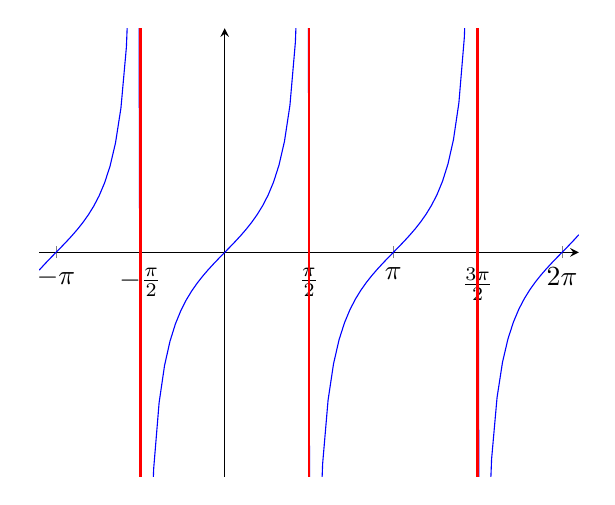
\begin{tikzpicture}
\begin{axis}[
  axis x line=center, axis y line=center,
  ymax=4.1,ymin=-4.1, ymajorticks=false,
  xtick={-3.141592654,-1.570796327,1.570796327,3.141592654,4.71238898,6.283185307},
  xticklabels={$-\pi$, $-\frac{\pi}{2}$, $\frac{\pi}{2}$, $\pi$, $\frac{3\pi}{2}$,$2\pi$}
  ]
\addplot[blue,domain=-1.1*pi:2.1*pi,samples=100] {tan(deg(x))};

\addplot[line width=1pt,red] coordinates {(-1.570796327,4.15) (-1.570796327,-4.15)};
\addplot[line width=1pt,red] coordinates {(1.570796327,4.15) (1.570796327,-4.15)};
\addplot[line width=1pt,red] coordinates {(4.71238898,4.15) (4.71238898,-4.15)};
\end{axis}
\end{tikzpicture}
\end{tabular}
\end{center}

\section{Trigonometry --- Special Triangles}\label{sec_A_6}
\begin{center}
  \includegraphics[height=4cm]{special_triangles}
\end{center}
From the above pair of special triangles we have
\begin{align*}
  \sin \frac{\pi}{4} &= \frac{1}{\sqrt{2}} &  \sin \frac{\pi}{6} &= \frac{1}{2} & \sin \frac{\pi}{3} &= \frac{\sqrt{3}}{2} \\
  \cos \frac{\pi}{4} &= \frac{1}{\sqrt{2}} &  \cos \frac{\pi}{6} &= \frac{\sqrt{3}}{2} & \cos \frac{\pi}{3} &= \frac{1}{2} \\
  \tan \frac{\pi}{4} &= 1 &  \tan \frac{\pi}{6} &= \frac{1}{\sqrt{3}} & \tan
\frac{\pi}{3} &= \sqrt{3}
\end{align*}

\section{Trigonometry --- Simple Identities}\label{sec_A_7}
\begin{itemize}
 \item Periodicity
\begin{align*}
  \sin(\theta+2\pi) &= \sin(\theta) &
  \cos(\theta+2\pi) &= \cos(\theta)
\end{align*}
\item Reflection
\begin{align*}
  \sin(-\theta)&=-\sin(\theta) & \cos(-\theta) &=\cos(\theta)
%   \sin(\pi-\theta)&=\sin(\theta) & \cos(\pi-\theta) &=\cos(\theta) \\
%   \sin(\pi+\theta)&=-\sin(\theta) & \cos(\pi+\theta) &=-\cos(\theta)
\end{align*}
\item Reflection around $\pi/4$
\begin{align*}
\sin\left(\tfrac{\pi}{2}-\theta\right)&=\cos\theta &
\cos\left(\tfrac{\pi}{2}-\theta\right)&=\sin\theta
\end{align*}
\item Reflection around $\pi/2$
\begin{align*}
\sin\left(\pi-\theta\right)&=\sin\theta &
\cos\left(\pi-\theta\right)&=-\cos\theta
\end{align*}
\item Rotation by $\pi$
\begin{align*}
\sin\left(\theta+\pi\right)&=-\sin\theta &
\cos\left(\theta+\pi\right)&=-\cos\theta
\end{align*}
\item Pythagoras
\begin{align*}
\sin^2\theta + \cos^2 \theta &=1
\end{align*}

\end{itemize}

\section{Trigonometry --- Add and Subtract Angles}\label{sec trig add}
\begin{itemize}
 \item Sine
\begin{align*}
  \sin(\alpha \pm \beta) &= \sin(\alpha)\cos(\beta) \pm \cos(\alpha)\sin(\beta)
  \end{align*}
 \item Cosine
\begin{align*}
  \cos(\alpha \pm \beta) &= \cos(\alpha)\cos(\beta) \mp \sin(\alpha)\sin(\beta)
\end{align*}

\end{itemize}

\section{Inverse Trigonometric Functions}\label{sec inv trig}
Some of you may not have studied inverse trigonometric functions in highschool, however
we still expect you to know them by the end of the course.
\begin{center}
\renewcommand{\arraystretch}{1.5}
\begin{tabular}{|c|c|c|}
\hline
$\arcsin x$ & $\arccos x$ & $\arctan x$\\
\hline
Domain: $-1 \leq x \leq 1$&
Domain: $-1 \leq x \leq 1$&
Domain: all real numbers\\
Range: $-\frac{\pi}{2} \leq \arcsin x \leq \frac{\pi}{2}$&
Range: $0 \leq \arccos x \leq \pi$&
Range: $-\frac{\pi}{2} < \arctan x < \frac{\pi}{2}$\\
\hline
\begin{tikzpicture} 
\begin{axis}[
  legend pos = north west,
  axis x line=center, axis y line=center, 
  xmax=1.1,xmin=-1.1, xtick={-1,1},
  ymin=-2, ymax=2,
  ytick={-1.570796327,1.570796327},
  yticklabels={$-\nicefrac{\pi}{2}$, $\nicefrac{\pi}{2}$}
  ]
\addplot[blue, line width=1pt, domain=-1:1,samples=100] {asin(x)/180*pi}; 
% \legend{$\arcsin \theta$}
\end{axis}
\end{tikzpicture}
&
\begin{tikzpicture} 
\useasboundingbox (0,0) rectangle (5,4.2);
\begin{axis}[
  axis x line=center, axis y line=center, 
  xmax=1.1,xmin=-1.1, xtick={-1,1},
  ymin=-0.3,ymax=3.4,
  ytick={0,1.570796327,3.141592654},
  yticklabels={0,$\nicefrac{\pi}{2}$, $\pi$}
  ]
 \addplot[blue, line width=1pt, domain=-1:1,samples=100] {acos(x)/180*pi}; 
% \legend{$\cos \theta$}
\end{axis}
\end{tikzpicture}
&
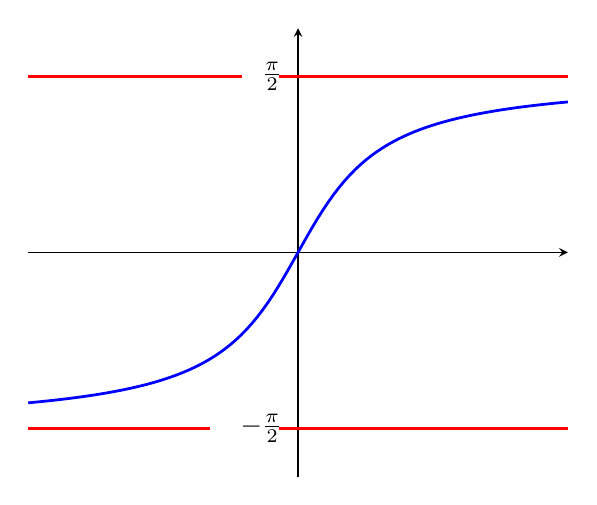
\begin{tikzpicture} 
\begin{axis}[
  legend pos = north west,
  axis x line=center, axis y line=center, 
  xmax=4.3,xmin=-4.3, xmajorticks=false,
  ymin=-2,ymax=2,
  ytick={-1.570796327,1.570796327},
  yticklabels={$-\frac{\pi}{2}$, $\frac{\pi}{2}$}
  ]
\addplot[blue, line width=1pt, domain=-4.3:4.3,samples=100] {atan(x)/180*pi}; 
% \legend{$\tan \theta$}

\addplot[line width=1pt,red] coordinates {(4.3,-1.570796327) (-0.3,-1.570796327)};
\addplot[line width=1pt,red] coordinates {(-1.4,-1.570796327) (-4.3,-1.570796327)};
\addplot[line width=1pt,red] coordinates {(4.3,1.570796327) (-0.3,1.570796327)};
\addplot[line width=1pt,red] coordinates {(-0.9,1.570796327) (-4.3,1.570796327)};
\end{axis}
\end{tikzpicture}
\\ \hline
\end{tabular}
\renewcommand{\arraystretch}{1}
\end{center}
Since these functions are inverses of each other we have
\begin{align*}
  \arcsin(\sin \theta) &= \theta & -\frac{\pi}{2} \leq \theta \leq \frac{\pi}{2} \\
  \arccos(\cos \theta) &= \theta & 0 \leq \theta \leq \pi \\
  \arctan(\tan \theta) &= \theta & -\frac{\pi}{2} \leq \theta \leq \frac{\pi}{2}	
\end{align*}
and also
\begin{align*}
  \sin(\arcsin x) &= x & -1 \leq x \leq 1 \\
  \cos(\arccos x) &= x & -1 \leq x \leq 1 \\
  \tan(\arctan x) &= x & \text{any real $x$}
\end{align*}
%The compositions of trignometric and inverse trigonometric functions are
%\begin{align*}
%  \sin( \arcsin x ) &= x & 
%  \sin( \arccos x ) &= \sqrt{1-x^2} & 
%  \sin( \arctan x ) &= \frac{x}{\sqrt{1+x^2}} \\ 
%%
%  \cos( \arcsin x ) &= \sqrt{1-x^2} & 
%  \cos( \arccos x ) &= x &
%  \cos( \arctan x ) &= \frac{1}{\sqrt{1+x^2}} \\ 
%%
%  \tan( \arcsin x ) &= \frac{x}{\sqrt{1-x^2}} & 
%  \tan( \arccos x ) &= \frac{\sqrt{1-x^2}}{x} &
%  \tan( \arctan x ) &= x 
%\end{align*}

\begin{center}
\renewcommand{\arraystretch}{1.5}
\begin{tabular}{|c|c|c|}
\hline
$\arccsc x$ & $\arcsec x$ & $\arccot x$\\
\hline
Domain: $|x|\ge 1$&
Domain: $|x|\ge 1$&
Domain: all real numbers\\
Range: $-\frac{\pi}{2} \leq \arccsc x \leq \frac{\pi}{2}$&
Range: $0 \leq \arcsec x \leq \pi$&
Range: $0 < \arccot x < \pi$\\[-0.1in]
       $\arccsc x \ne 0$ &
       $\arcsec x \ne \frac{\pi}{2}$ &
        \\
\hline
\begin{tikzpicture} 
\begin{axis}[
  legend pos = north west,
  axis x line=center, axis y line=center, 
  xmax=4.3,xmin=-4.3, xtick={-1,1},
  ymin=-2, ymax=2,
  ytick={-1.570796327,1.570796327},
  yticklabels={$-\frac{\pi}{2}\!\!\!$, $\frac{\pi}{2}$}
  ]
\addplot[blue, line width=1pt, domain=1:4.3,samples=50] {asin(1/x)/180*pi}; 
\addplot[blue, line width=1pt, domain=-4.3:-1,samples=50] {asin(1/x)/180*pi}; 
\end{axis}
\end{tikzpicture}
&
\begin{tikzpicture} 
\useasboundingbox (0,0) rectangle (5,4.2);
\begin{axis}[
  axis x line=center, axis y line=center, 
  xmax=4.3,xmin=-4.3, xtick={-1,1},
  ymin=-0.3,ymax=3.4,
  ytick={0,1.570796327,3.141592654},
  yticklabels={0,$\frac{\pi}{2}$, $\pi$}
  ]
 \addplot[blue, line width=1pt, domain=1:4.3,samples=100] {acos(1/x)/180*pi}; 
 \addplot[blue, line width=1pt, domain=-4.3:-1,samples=100] {acos(1/x)/180*pi}; 
% \legend{$\cos \theta$}
\end{axis}
\end{tikzpicture}
&
\begin{tikzpicture} 
\begin{axis}[
  legend pos = north west,
  axis x line=center, axis y line=center, 
  xmax=4.3,xmin=-4.3, xmajorticks=false,
  ymin=-0.3,ymax=3.4,
  ytick={0,1.570796327,3.141592654},
  yticklabels={0,$\frac{\pi}{2}$, $\pi$}
  ]
\addplot[blue, line width=1pt, domain=-4.3:-0.01,samples=100] {atan(1/x)/180*pi + pi}; 
\addplot[blue, line width=1pt, domain=0.01:4.3,samples=100] {atan(1/x)/180*pi}; 
% \legend{$\tan \theta$}

\addplot[line width=1pt,red] coordinates {(4.3,3.141592654) (-0.3,3.141592654)};
\addplot[line width=1pt,red] coordinates {(-0.9,3.141592654) (-4.3,3.141592654)};
\end{axis}
\end{tikzpicture}
\\ \hline
\end{tabular}
\renewcommand{\arraystretch}{1}
\end{center}
Again
\begin{align*}
  \arccsc(\csc \theta) &= \theta & -\frac{\pi}{2} \leq \theta \leq \frac{\pi}{2},\ \theta\ne 0 \\
  \arcsec(\sec \theta) &= \theta & 0 \leq \theta \leq \pi,\ \theta\ne \frac{\pi}{2} \\
  \arccot(\cot \theta) &= \theta & 0 < \theta < \pi	
\end{align*}
and 
\begin{align*}
  \csc(\arccsc x) &= x & |x|\ge 1 \\
  \sec(\arcsec x) &= x & |x|\ge 1 \\
  \cot(\arccot x) &= x & \text{any real $x$}
\end{align*}

\section{Areas}\label{app sec areas}
\begin{center}
 \includegraphics[width=\textwidth]{area2d}
\end{center}
\begin{itemize}
 \item Area of a rectangle
\begin{align*}
  A &= b h
\end{align*}
 \item Area of a triangle
\begin{align*}
  A &= \frac{1}{2} b h = \frac{1}{2} ab \sin \theta
\end{align*}
 \item Area of a circle
\begin{align*}
  A &= \pi r^2
\end{align*}
 \item Area of an ellipse
\begin{align*}
  A &= \pi ab
\end{align*}
\end{itemize}

\section{Volumes}\label{sec volumes}
\begin{center}
 \includegraphics[width=\textwidth]{vol3d}
\end{center}
\begin{itemize}
 \item Volume of a rectangular prism
\begin{align*}
  V &= l w h
\end{align*}
 \item Volume of a cylinder
\begin{align*}
  V &= \pi r^2 h
\end{align*}
 \item Volume of a cone
\begin{align*}
  V &= \frac{1}{3} \pi r^2 h
\end{align*}

 \item Volume of a sphere
\begin{align*}
  V &= \frac{4}{3} \pi r^3
\end{align*}
\end{itemize}


\section{Powers}\label{sec powers}
In the following, $x$ and $y$ are arbitrary real numbers,
and $q$ is an arbitrary constant that is strictly bigger
than zero.
\begin{itemize}
 \item $q^0=1$

\item $q^{x+y}=q^xq^y$,
         $q^{x-y}=\frac{q^x}{q^y}$
\item $q^{-x}=\frac{1}{q^x}$
\item $\big(q^x\big)^y=q^{xy}$
\item  $\lim\limits_{x\rightarrow\infty}q^x=\infty$,
           $\lim\limits_{x\rightarrow-\infty}q^x=0$ if $q>1$
\item $\lim\limits_{x\rightarrow\infty}q^x=0$,
           $\lim\limits_{x\rightarrow-\infty}q^x=\infty$ if $0<q<1$
\item  The graph of $2^x$ is given below. The graph of  $q^x$,
for any $q>1$, is similar.

\begin{center}
\includegraphics{expGraph2}
\end{center}


\end{itemize}


\section{Logarithms}\label{sec logs}

In the following, $x$ and $y$ are arbitrary real numbers that
are strictly bigger than 0, and
$p$ and $q$ are arbitrary constants that are strictly bigger than one.

\begin{itemize}
\item   $q^{\log_q x}=x$,\ \ \
            $\log_q \big(q^x\big)=x$
\item   $\log_q x=\frac{\log_p x}{\log_p q}$
\item  $\log_q 1=0$,\ \ \
          $\log_q q=1$
\item $\log_q(xy)=\log_q x+\log_q y$
\item $\log_q\big(\frac{x}{y}\big)=\log_q x-\log_q y$
\item $\log_q\big(\frac{1}{y}\big)=-\log_q y$,
\item $\log_q(x^y)=y\log_q x$
\item $\lim\limits_{x\rightarrow\infty}\log_q x=\infty$, \ \ \
           $\lim\limits_{x\rightarrow0+}\log_q x=-\infty$
\item The graph of $\log_{10} x$ is given below. The graph of  $\log_q x$,
for any $q>1$, is similar.

\begin{center}
\includegraphics{logGraph10}
\end{center}

\end{itemize}



\longsection{Highschool Material You Should be Able to Derive}{You should be
able to derive}
\label{sec must deriv}
\begin{itemize}
 \item Graphs of $\csc\theta, \sec \theta$ and $\cot \theta$:
\end{itemize}
\begin{center}
\begin{tabular}{ccc}
$\csc \theta$ & $\sec \theta$ & $\cot \theta$ \\
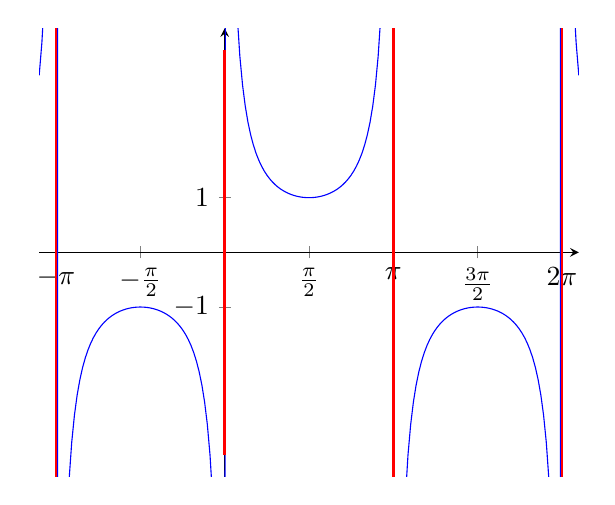
\begin{tikzpicture}
\begin{axis}[
  axis x line=center, axis y line=center,
  ymax=4.1,ymin=-4.1,ytick={-1,1},
  xtick={-3.141592654,-1.570796327,1.570796327,3.141592654,4.71238898,6.283185307},
  xticklabels={$-\pi$, $-\frac{\pi}{2}$, $\frac{\pi}{2}$, $\pi$, $\frac{3\pi}{2}$,$2\pi$}
  ]
\addplot[blue,domain=-1.1*pi:2.1*pi,samples=200] {cosec(deg(x))};
% \legend{$\csc \theta$}

\addplot[line width=1pt,red] coordinates {(-3.141592654,4.15) (-3.141592654,-4.15)};
\addplot[line width=1pt,red] coordinates {(0,3.7) (0,-3.7)};
\addplot[line width=1pt,red] coordinates {(3.141592654,4.15) (3.141592654,-4.15)};
\addplot[line width=1pt,red] coordinates {(6.283185307,4.15) (6.283185307,-4.15)};
\end{axis}
\end{tikzpicture}
&
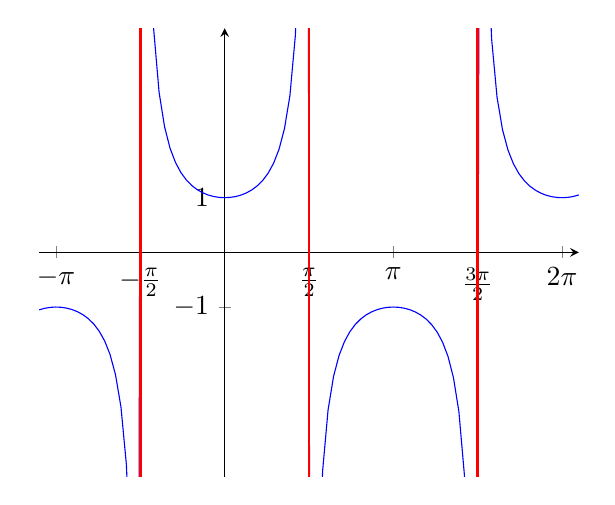
\begin{tikzpicture}
\begin{axis}[
  axis x line=center, axis y line=center,
  ymax=4.1,ymin=-4.1, ytick={-1,1},
  xtick={-3.141592654,-1.570796327,1.570796327,3.141592654,4.71238898,6.283185307},
  xticklabels={$-\pi$, $-\frac{\pi}{2}$, $\frac{\pi}{2}$, $\pi$, $\frac{3\pi}{2}$,$2\pi$}
  ]
\addplot[blue,domain=-1.1*pi:2.1*pi,samples=100] {sec(deg(x))};
% \legend{$\sec \theta$}
\addplot[line width=1pt,red] coordinates {(-1.570796327,4.15) (-1.570796327,-4.15)};
\addplot[line width=1pt,red] coordinates {(1.570796327,4.15) (1.570796327,-4.15)};
\addplot[line width=1pt,red] coordinates {(4.71238898,4.15) (4.71238898,-4.15)};

\end{axis}
\end{tikzpicture}
&
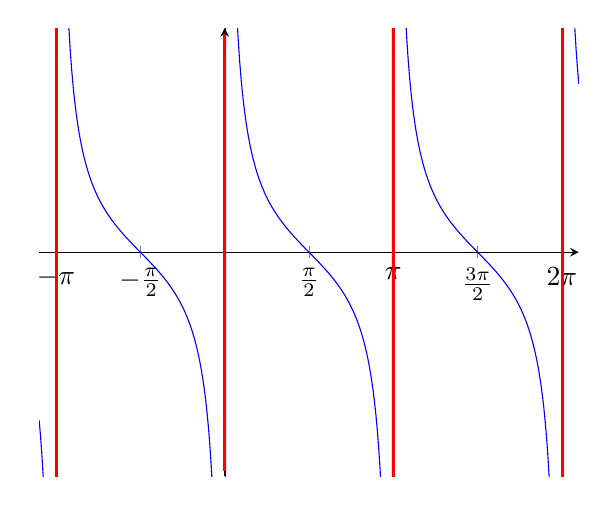
\begin{tikzpicture}
\begin{axis}[
  axis x line=center, axis y line=center,
  ymax=4.1,ymin=-4.1, ymajorticks=false,
  xtick={-3.141592654,-1.570796327,1.570796327,3.141592654,4.71238898,6.283185307},
  xticklabels={$-\pi$, $-\frac{\pi}{2}$, $\frac{\pi}{2}$, $\pi$, $\frac{3\pi}{2}$,$2\pi$}
  ]
\addplot[blue,domain=-1.1*pi:2.1*pi,samples=400] {cot(deg(x))};
% \legend{$\cot \theta$}

\addplot[line width=1pt,red] coordinates {(-3.14,4.15) (-3.14,-4.15)};
\addplot[line width=1pt,red] coordinates {(0,4) (0,-4)};
\addplot[line width=1pt,red] coordinates {(3.14,4.15) (3.14,-4.15)};
\addplot[line width=1pt,red] coordinates {(6.3,4.15) (6.3,-4.15)};
\end{axis}
\end{tikzpicture}
\end{tabular}
\end{center}
\begin{itemize}
 \item More Pythagoras
\begin{align*}
\sin^2\theta + \cos^2 \theta &=1 & \xmapsto{\text{divide by $\cos^2\theta$}}&&
\tan^2\theta + 1  &= \sec^2\theta \\
\sin^2\theta + \cos^2 \theta &=1 & \xmapsto{\text{divide by $\sin^2\theta$}}&&
1 + \cot^2 \theta &=\csc^2\theta
\end{align*}

 \item Sine --- double angle (set $\beta =\alpha$ in sine angle addition formula)
\begin{align*}
  \sin(2\alpha) &= 2\sin(\alpha)\cos(\alpha)
\end{align*}
 \item Cosine --- double angle (set $\beta =\alpha$ in cosine angle addition formula)
\begin{align*}
  \cos(2\alpha) &= \cos^2(\alpha) - \sin^2(\alpha) \\
  &= 2\cos^2(\alpha) - 1  & \text{(use $\sin^2(\alpha)= 1-\cos^2(\alpha)$)}\\
  &= 1 - 2\sin^2(\alpha) & \text{(use $\cos^2(\alpha)= 1-\sin^2(\alpha)$)}
\end{align*}
% \item Tangent --- double angle (use the two previous double-angle identities)
% \begin{align*}
%   \tan( 2 \alpha) &= \frac{2\sin(\alpha)\cos(\alpha)}{\cos^2(\alpha) - \sin^2(\alpha)}
%   & \text{now divide numerator and denominator by $\cos^2(\alpha)$}\\
%   &= \frac{2 \tan(\alpha) }{1 - \tan^2(\alpha)}
% \end{align*}
\item Composition of trigonometric and inverse trigonometric functions:
\begin{align*}
  \cos( \arcsin x) &= \sqrt{1-x^2} &
  \sec( \arctan x) &= \sqrt{1+x^2}
\end{align*}
and similar expressions.
\end{itemize}

\chapter{Origin of Trig, Area and Volume Formulas}\label{chap_app_B}
\section{Theorems about Triangles}\label{sec_B_1}
\subsection{Thales' Theorem}\label{ssec_B_1_1}
We want to get at right-angled triangles. A classic construction for this is to
draw a triangle inside a circle, so that all three corners lie on the circle
and the longest side forms the diameter of the circle. See the figure below in
which we have scaled the circle to have radius 1 and the triangle has longest
side 2.

\begin{center}
  \includegraphics[height=4cm]{thales}
\end{center}

Thales theorem states that the angle at $C$ is always a right-angle. The proof
is quite straight-forward and relies on two facts:
\begin{itemize}
 \item the angles of a triangle add to $\pi$, and
 \item the angles at the base of an isosceles triangle are equal.
\end{itemize}
So we split the triangle $ABC$ by drawing a line from the centre of the circle to $C$. This creates two isosceles triangles $OAC$ and $OBC$. Since they are isosceles, the angles at their bases $\alpha$ and $\beta$ must be equal (as shown).  Adding the angles of the original triangle now gives
\begin{align*}
  \pi &= \alpha + (\alpha+\beta) + \beta = 2(\alpha+\beta)
\end{align*}
So the angle at $C = \pi - (\alpha+\beta) = \pi/2$.


\subsection{Pythagoras}\label{ssec_B_1_2}
Since trigonometry, at its core, is the study of lengths and angles in right-angled
triangles, we must include a result you all know well, but likely do not know how to
prove.
\begin{center}
  \includegraphics[height=3.5cm]{right_triangle}
\end{center}
The lengths of the sides of any right-angled triangle are related by the famous result due to Pythagoras
\begin{align*}
  c^2 &= a^2+b^2.
\end{align*}
There are many ways to prove this, but we can do so quite simply by studying the following diagram:
\begin{center}
  \includegraphics[height=4cm]{pythag}
\end{center}
We start with a right-angled triangle with sides labeled $a,b$ and $c$. Then we construct a square of side-length $a+b$ and draw inside it 4 copies of the triangle arranged as shown in the centre of the above figure. The area in white is then $a^2+b^2$. Now move the triangles around to create the arrangement shown on the right of the above figure. The area in white is bounded by a square of side-length $c$ and so its area is $c^2$. The area of the outer square didn't change when the triangles were moved, nor did the area of the triangles, so the white area cannot have changed either. This proves $a^2+b^2=c^2$.


\section{Trigonometry}\label{sec_B_2}
\subsection{Angles --- Radians vs Degrees}\label{ssec rad deg}
For mathematics, and especially in calculus, it is much better to measure angles in units
called radians rather than degrees. By definition, an arc of length $\theta$ on a circle
of radius one subtends an angle of $\theta$ radians at the centre of the
circle.
\begin{center}
 \includegraphics[height=4cm]{radian}
\end{center}
The circle on the left has radius 1, and the arc swept out by an angle of
$\theta$ radians has length~$\theta$. Because a circle of radius one has circumference
$2\pi$ we have
\begin{align*}
   2\pi\text{ radians }&=360^\circ &
    \pi\text{ radians }&=180^\circ &
    \nicefrac{\pi}{2}\text{ radians }&=90^\circ \\
%%
  \frac{\pi}{3}\text{ radians }&=60^\circ &
  \frac{\pi}{4}\text{ radians }&=45^\circ &
  \frac{\pi}{6}\text{ radians }&=30^\circ
\end{align*}

More generally, consider a circle of radius $r$. Let $L(\theta)$ denote the length of
the arc swept out by an angle of $\theta$ radians and let $A(\theta)$ denote the area of
the sector (or wedge) swept out by the same angle. Since the angle sweeps out the
fraction $\nicefrac{\theta}{2\pi}$ of a whole circle, we have
\begin{align*}
  L(\theta) &= 2\pi r \cdot \frac{\theta}{2\pi} = \theta r & \text{and}\\
  A(\theta) &= \pi r^2 \cdot \frac{\theta}{2\pi} = \frac{\theta}{2} r^2
\end{align*}

\subsection{Trig Function Definitions}\label{ssec_B_2_2}
The trigonometric functions are defined as ratios of the lengths of the sides of a
right-angle triangle as shown in the left of the diagram below . These ratios depend only
on the angle~$\theta$.
\begin{center}
  \includegraphics[height=5cm]{trig_defn}
\end{center}
The trigonometric functions sine, cosine and tangent are defined as ratios of
the lengths of the sides
\begin{align*}
% \text{sine} && \text{cosine} && \text{tangent}\\
\sin\theta &= \frac{\text{opposite}}{\text{hypotenuse}} &
\cos\theta &= \frac{\text{adjacent}}{\text{hypotenuse}} &
\tan\theta &= \frac{\text{opposite}}{\text{adjacent}} = \frac{\sin \theta}{\cos \theta}.
\intertext{These are frequently abbreviated as}
\sin\theta &= \frac{\text{o}}{\text{h}} &
\cos\theta &= \frac{\text{a}}{\text{h}} &
\tan\theta &= \frac{\text{o}}{\text{a}}
\end{align*}
which gives rise to the mnemonic
\begin{align*}
  \text{SOH} && \text{CAH} && \text{TOA}
\end{align*}
If we scale the triangle so that they hypotenuse has length $1$ then we obtain the
diagram on the right. In that case, $\sin \theta$ is the height of the triangle, $\cos
\theta$ the length of its base and $\tan \theta$ is the length of the line tangent to the
circle of radius 1 as shown.

Since the angle $2\pi$ sweeps out a full circle, the angles $\theta$ and $\theta+2\pi$
are really the same.
\begin{center}
  \includegraphics[height=5cm]{trig_defn3}
\end{center}
Hence all the trigonometric functions are periodic with period $2\pi$. That is
\begin{align*}
  \sin(\theta+2\pi) &= \sin(\theta) &
  \cos(\theta+2\pi) &= \cos(\theta) &
  \tan(\theta+2\pi) &= \tan(\theta)
\end{align*}
The plots of these functions are shown below
\begin{center}
\begin{tabular}{ccc}
$\sin \theta$ & $\cos \theta$ & $\tan \theta$
\\
\begin{tikzpicture}
\begin{axis}[
  axis x line=center, axis y line=center,
  ymax=1.1,ymin=-1.1, ytick={-1,1},
  xtick={-3.141592654,-1.570796327,1.570796327,3.141592654,4.71238898,6.283185307},
  xticklabels={$-\pi$, $-\frac{\pi}{2}$, $\frac{\pi}{2}$, $\pi$, $\frac{3\pi}{2}$,$2\pi$}
  ]
\addplot[blue,domain=-1.1*pi:2.1*pi,samples=100] {sin(deg(x))};
\end{axis}
\end{tikzpicture}
&
\begin{tikzpicture}
\begin{axis}[
  axis x line=center, axis y line=center,
  ymax=1.1,ymin=-1.1, ytick={-1,1},
  xtick={-3.141592654,-1.570796327,1.570796327,3.141592654,4.71238898,6.283185307},
  xticklabels={$-\pi$, $-\frac{\pi}{2}$, $\frac{\pi}{2}$, $\pi$, $\frac{3\pi}{2}$,$2\pi$}
  ]
\addplot[blue,domain=-1.1*pi:2.1*pi,samples=100] {cos(deg(x))};
\end{axis}
\end{tikzpicture}
&
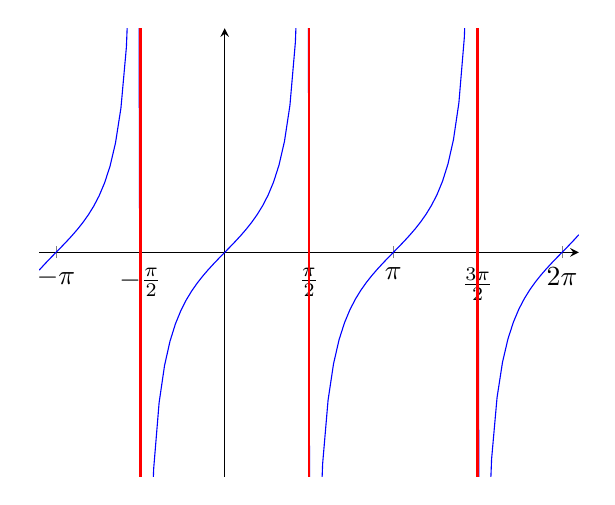
\begin{tikzpicture}
\begin{axis}[
  axis x line=center, axis y line=center,
  ymax=4.1,ymin=-4.1, ymajorticks=false,
  xtick={-3.141592654,-1.570796327,1.570796327,3.141592654,4.71238898,6.283185307},
  xticklabels={$-\pi$, $-\frac{\pi}{2}$, $\frac{\pi}{2}$, $\pi$, $\frac{3\pi}{2}$,$2\pi$}
  ]
\addplot[blue,domain=-1.1*pi:2.1*pi,samples=100] {tan(deg(x))};

\addplot[line width=1pt,red] coordinates {(-1.570796327,4.15) (-1.570796327,-4.15)};
\addplot[line width=1pt,red] coordinates {(1.570796327,4.15) (1.570796327,-4.15)};
\addplot[line width=1pt,red] coordinates {(4.71238898,4.15) (4.71238898,-4.15)};
\end{axis}
\end{tikzpicture}
\end{tabular}
\end{center}


The reciprocals (cosecant, secant and cotangent) of these functions also play important
roles in trigonometry and calculus:
\begin{align*}
% \text{cosecant} && \text{secant} && \text{cotangent}\\
\csc \theta &= \frac{1}{\sin\theta} = \frac{\text{h}}{\text{o}} &
\sec\theta &= \frac{1}{\cos \theta} = \frac{\text{h}}{\text{a}} &
\cot\theta &= \frac{1}{\tan \theta} = \frac{\cos \theta}{\sin\theta} =
\frac{\text{a}}{\text{o}}
\end{align*}
The plots of these functions are shown below
\begin{center}
\begin{tabular}{ccc}
$\csc \theta$ & $\sec \theta$ & $\cot \theta$ \\
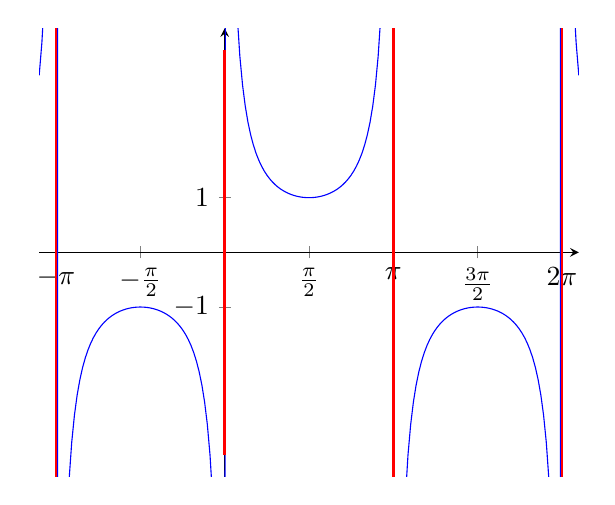
\begin{tikzpicture}
\begin{axis}[
  axis x line=center, axis y line=center,
  ymax=4.1,ymin=-4.1,ytick={-1,1},
  xtick={-3.141592654,-1.570796327,1.570796327,3.141592654,4.71238898,6.283185307},
  xticklabels={$-\pi$, $-\frac{\pi}{2}$, $\frac{\pi}{2}$, $\pi$, $\frac{3\pi}{2}$,$2\pi$}
  ]
\addplot[blue,domain=-1.1*pi:2.1*pi,samples=200] {cosec(deg(x))};
% \legend{$\csc \theta$}

\addplot[line width=1pt,red] coordinates {(-3.141592654,4.15) (-3.141592654,-4.15)};
\addplot[line width=1pt,red] coordinates {(0,3.7) (0,-3.7)};
\addplot[line width=1pt,red] coordinates {(3.141592654,4.15) (3.141592654,-4.15)};
\addplot[line width=1pt,red] coordinates {(6.283185307,4.15) (6.283185307,-4.15)};
\end{axis}
\end{tikzpicture}
&
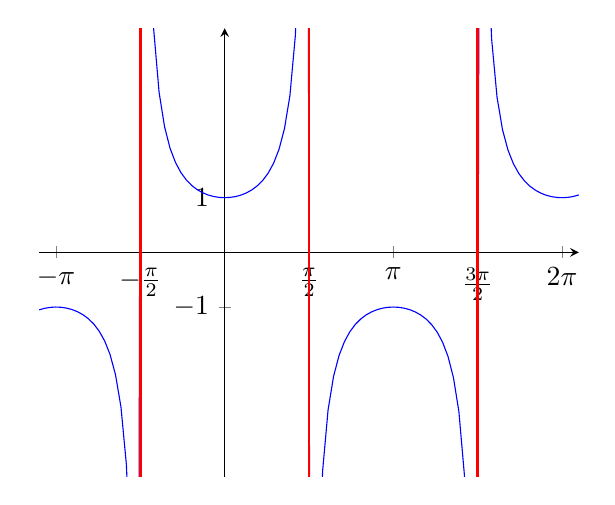
\begin{tikzpicture}
\begin{axis}[
  axis x line=center, axis y line=center,
  ymax=4.1,ymin=-4.1, ytick={-1,1},
  xtick={-3.141592654,-1.570796327,1.570796327,3.141592654,4.71238898,6.283185307},
  xticklabels={$-\pi$, $-\frac{\pi}{2}$, $\frac{\pi}{2}$, $\pi$, $\frac{3\pi}{2}$,$2\pi$}
  ]
\addplot[blue,domain=-1.1*pi:2.1*pi,samples=100] {sec(deg(x))};
% \legend{$\sec \theta$}
\addplot[line width=1pt,red] coordinates {(-1.570796327,4.15) (-1.570796327,-4.15)};
\addplot[line width=1pt,red] coordinates {(1.570796327,4.15) (1.570796327,-4.15)};
\addplot[line width=1pt,red] coordinates {(4.71238898,4.15) (4.71238898,-4.15)};

\end{axis}
\end{tikzpicture}
&
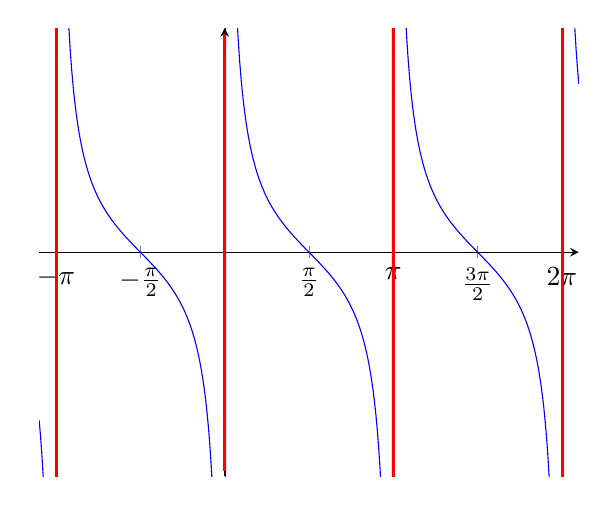
\begin{tikzpicture}
\begin{axis}[
  axis x line=center, axis y line=center,
  ymax=4.1,ymin=-4.1, ymajorticks=false,
  xtick={-3.141592654,-1.570796327,1.570796327,3.141592654,4.71238898,6.283185307},
  xticklabels={$-\pi$, $-\frac{\pi}{2}$, $\frac{\pi}{2}$, $\pi$, $\frac{3\pi}{2}$,$2\pi$}
  ]
\addplot[blue,domain=-1.1*pi:2.1*pi,samples=400] {cot(deg(x))};
% \legend{$\cot \theta$}

\addplot[line width=1pt,red] coordinates {(-3.14,4.15) (-3.14,-4.15)};
\addplot[line width=1pt,red] coordinates {(0,4) (0,-4)};
\addplot[line width=1pt,red] coordinates {(3.14,4.15) (3.14,-4.15)};
\addplot[line width=1pt,red] coordinates {(6.3,4.15) (6.3,-4.15)};
\end{axis}
\end{tikzpicture}
\end{tabular}
\end{center}



These reciprocal functions also have geometric interpretations:
\begin{center}
  \includegraphics[height=6cm]{trig_defn2}
\end{center}
Since these are all right-angled triangles we can use Pythagoras to obtain the following
identities:
\begin{align*}
\sin^2\theta + \cos^2 \theta &=1 &
\tan^2\theta + 1  &= \sec^2\theta &
1 + \cot^2 \theta &=\csc^2\theta
\end{align*}
Of these it is only necessary to remember the first
\begin{align*}
\sin^2\theta + \cos^2 \theta &=1
\end{align*}
The second can then be obtained by dividing this by $\cos^2\theta$ and the third by
dividing by $\sin^2\theta$.


\subsection{Important Triangles}\label{ssec_B_2_3}
Computing sine and cosine is non-trivial for general angles --- we need Taylor series (or
similar tools) to do this. However there are some special angles (usually small
integer fractions of $\pi$) for which we can use a little geometry to help. Consider the
following two triangles.
\begin{center}
  \includegraphics[height=4cm]{special_triangles}
\end{center}
The first results from cutting a square along its diagonal, while the second is obtained
by cutting an equilateral triangle from one corner to the middle of the opposite side.
These, together with the angles $0,\frac{\pi}{2}$ and $\pi$ give the following table of
values
\begin{center}
\renewcommand{\arraystretch}{1.3}
     \begin{tabular}{|c||c|c|c||c|c|c|}
          \hline
         $\theta$ & $\sin\theta$ & $\cos\theta$ & $\tan\theta$  &
                    $\csc\theta$ & $\sec\theta$ & $\cot\theta$   \\  \hline\hline
%%
        $0$ rad & 0 & 1 & 0 & DNE & 1 & DNE  \\ \hline
        $\tfrac{\pi}{2}$ rad  & 1 & 0  & DNE & 1& DNE & 0 \\ \hline
        $\pi$ rad & 0 & -1 & 0 & DNE & -1 & DNE \\ \hline\hline
%%
         $\tfrac{\pi}{4}$ rad &
            $\tfrac{1}{\sqrt{2}}$ & $\tfrac{1}{\sqrt{2}}$ & 1 &
            $\sqrt{2}$ & $\sqrt{2}$ & 1 \\ \hline\hline
%%
        $\tfrac{\pi}{6}$ rad &
            $\tfrac{1}{2}$ & $\tfrac{\sqrt{3}}{2}$ & $\tfrac{1}{\sqrt{3}}$ &
            2 & $\tfrac{2}{\sqrt{3}}$ & $\sqrt{3}$  \\ \hline
        $\tfrac{\pi}{3}$ rad &
            $\tfrac{\sqrt{3}}{2}$ & $\tfrac{1}{2}$ & $\sqrt{3}$ &
            $\tfrac{2}{\sqrt{3}}$ &  2 & $\tfrac{1}{\sqrt{3}}$  \\ \hline
     \end{tabular}
\renewcommand{\arraystretch}{1.0}
\end{center}




\subsection{Some More Simple Identities}\label{ssec_B_2_4}
Consider the figure below
\begin{center}
 \includegraphics[height=55mm]{trig_defn4}
\end{center}
The pair triangles on the left shows that there is a simple relationship between
trigonometric functions evaluated at $\theta$ and at $-\theta$:
\begin{align*}
  \sin(-\theta)&=-\sin(\theta) & \cos(-\theta) &=\cos(\theta)
\end{align*}
That is --- sine is an odd function, while cosine is even. Since the other trigonometric
functions can be expressed in terms of sine and cosine we obtain
\begin{align*}
  \tan(-\theta) &=-\tan(\theta) &
  \csc(-\theta) &=-\csc(\theta) &
  \sec(-\theta) &=\sec(\theta) &
  \cot(-\theta) &=-\cot(\theta)
\end{align*}
Now consider the triangle on the right --- if we consider the angle
$\frac{\pi}{2}-\theta$ the side-lengths of the triangle remain unchanged, but the roles
of ``opposite'' and ``adjacent'' are swapped. Hence we have
\begin{align*}
\sin\left(\tfrac{\pi}{2}-\theta\right)&=\cos\theta &
\cos\left(\tfrac{\pi}{2}-\theta\right)&=\sin\theta
\end{align*}
Again these imply that
\begin{align*}
\tan\left(\tfrac{\pi}{2}-\theta\right)&=\cot\theta &
\csc\left(\tfrac{\pi}{2}-\theta\right)&=\sec\theta &
\sec\left(\tfrac{\pi}{2}-\theta\right)&=\csc\theta &
\cot\left(\tfrac{\pi}{2}-\theta\right)&=\tan\theta
\end{align*}

We can go further. Consider the following diagram:
\begin{center}
 \includegraphics[height=55mm]{trig_defn5}
\end{center}
This implies that
\begin{align*}
  \sin(\pi-\theta)&=\sin(\theta) & \cos(\pi-\theta) &= -\cos(\theta) \\
  \sin(\pi+\theta)&=-\sin(\theta) & \cos(\pi+\theta) &=-\cos(\theta)
\end{align*}
From which we can get the rules for the other four trigonometric functions.


\subsection{Identities --- Adding Angles}\label{ssec_B_2_5}
We wish to explain the origins of the identity
\begin{align*}
  \sin(\alpha+\beta) &= \sin(\alpha)\cos(\beta) + \cos(\alpha)\sin(\beta).
\end{align*}
A very geometric demonstration uses the figure below and an observation about areas.
\begin{center}
 \includegraphics[width=\textwidth]{add_angles}
\end{center}
\begin{itemize}
 \item  The left-most figure shows two right-angled triangles with angles $\alpha$ and $\beta$ and both with hypotenuse length $1$.
 \item The next figure simply rearranges the triangles --- translating and rotating the lower triangle so that it lies adjacent to the top of the upper triangle.
 \item Now scale the lower triangle by a factor of $q$ so that edges opposite the angles $\alpha$ and $\beta$ are flush. This means that $q \cos \beta = \cos \alpha$. ie
\begin{align*}
  q &= \frac{\cos\alpha}{\cos\beta}
\end{align*}
  Now compute the areas of these (blue and red) triangles
  \begin{align*}
  A_\text{red} &= \frac{1}{2} q^2 \sin\beta \cos \beta \\
  A_\text{blue} &= \frac{1}{2} \sin \alpha \cos \alpha
\intertext{So twice the total area is}
  2 A_\text{total} &= \sin \alpha \cos \alpha  + q^2 \sin\beta \cos \beta
\end{align*}
\item But we can also compute the total area using the rightmost triangle:
\begin{align*}
  2 A_\text{total} &= q \sin(\alpha+\beta)
\end{align*}
\end{itemize}
Since the total area must be the same no matter how we compute it we have
\begin{align*}
q \sin(\alpha+\beta) &=  \sin \alpha \cos \alpha  + q^2 \sin\beta \cos \beta \\
  \sin(\alpha+\beta) &= \frac{1}{q} \sin \alpha \cos \alpha + q \sin\beta \cos \beta \\
  &= \frac{\cos \beta}{\cos \alpha} \sin \alpha \cos \alpha + \frac{\cos \alpha}{\cos \beta} \sin\beta \cos \beta \\
  &= \sin \alpha \cos \beta +  \cos \alpha \sin\beta
\end{align*}
as required.

We can obtain the angle addition formula for cosine by substituting $\alpha \mapsto \pi/2-\alpha$ and $\beta \mapsto -\beta$ into our sine formula:
\begin{align*}
  \sin(\alpha+\beta) &= \sin(\alpha)\cos(\beta) + \cos(\alpha)\sin(\beta) & \text{becomes}\\
  \underbrace{\sin(\pi/2-\alpha-\beta)}_{\cos(\alpha+\beta)} &= \underbrace{\sin(\pi/2-\alpha)}_{\cos(\alpha)}\cos(-\beta) + \underbrace{\cos(\pi/2-\alpha)}_{\sin(\alpha)}\sin(-\beta) \\
  \cos(\alpha+\beta) &= \cos(\alpha)\cos(\beta) - \sin(\alpha)\sin(\beta)
\end{align*}
where we have used $\sin(\pi/2-\theta)=\cos(\theta)$ and $\cos(\pi/2-\theta)=\sin(\theta)$.

It is then a small step to the formulas for the difference of angles. From the relation
\begin{align*}
  \sin(\alpha+\beta) &= \sin(\alpha)\cos(\beta) + \cos(\alpha)\sin(\beta)
\end{align*}
we can substitute $\beta \mapsto -\beta$ and so obtain
\begin{align*}
  \sin(\alpha - \beta) &= \sin(\alpha)\cos(-\beta) + \cos(\alpha)\sin(-\beta)  \\
  &= \sin(\alpha)\cos(\beta) - \cos(\alpha)\sin(\beta)
\end{align*}
The formula for cosine can be obtained in a similar manner. To summarise
\begin{align*}
  \sin(\alpha \pm \beta) &= \sin(\alpha)\cos(\beta) \pm \cos(\alpha)\sin(\beta)\\
  \cos(\alpha \pm \beta) &= \cos(\alpha)\cos(\beta) \mp \sin(\alpha)\sin(\beta)
\end{align*}

The formulas for tangent are a bit more work, but
\begin{align*}
  \tan(\alpha + \beta) &= \frac{\sin(\alpha + \beta)}{\cos(\alpha + \beta)}\\
  &= \frac{\sin(\alpha)\cos(\beta) + \cos(\alpha)\sin(\beta)}{\cos(\alpha)\cos(\beta) - \sin(\alpha)\sin(\beta) }\\
  &= \frac{\sin(\alpha)\cos(\beta) + \cos(\alpha)\sin(\beta)}{\cos(\alpha)\cos(\beta) - \sin(\alpha)\sin(\beta) }
  \cdot \frac{\sec(\alpha) \sec(\beta)}{\sec(\alpha) \sec(\beta)} \\
  &= \frac{\sin(\alpha)\sec(\alpha) + \sin(\beta)\sec(\beta)}{1 - \sin(\alpha)\sec(\alpha)\sin(\beta)\sec(\beta) } \\
  &= \frac{\tan(\alpha) + \tan(\beta)}{1 - \tan(\alpha)\tan(\beta) }
\intertext{and similarly we get}
  \tan(\alpha - \beta) &=  \frac{\tan(\alpha) - \tan(\beta)}{1 + \tan(\alpha)\tan(\beta) }
\end{align*}

\subsection{Identities --- Double-angle Formulas}\label{ssec_B_2_6}
If we set $\beta=\alpha$ in the angle-addition formulas we get
\begin{align*}
  \sin(2\alpha) &= 2\sin(\alpha)\cos(\alpha) \\
  \cos(2\alpha) &= \cos^2(\alpha)-\sin^2(\alpha) \\
  &= 2\cos^2(\alpha)-1 & \text{since } \sin^2\theta =1-\cos^2\theta \\
  &= 1-2\sin^2(\alpha) & \text{since } \cos^2\theta =1-\sin^2\theta \\
  \tan(2\alpha) &= \frac{2\tan(\alpha)}{1-\tan^2(\alpha)} \\
  &= \frac{2}{\cot(\alpha)-\tan(\alpha)} &\text{divide top and bottom by
$\tan(\alpha)$}
\end{align*}

\subsection{Identities --- Extras}\label{ssec_B_2_7}
\subsubsection{Sums to Products}
Consider the identities
\begin{align*}
\sin(\alpha+\beta) &= \sin(\alpha)\cos(\beta) + \cos(\alpha) \sin(\beta) &
\sin(\alpha-\beta) &= \sin(\alpha)\cos(\beta) - \cos(\alpha) \sin(\beta)
\end{align*}
If we add them together some terms on the right-hand side cancel:
\begin{align*}
\sin(\alpha+\beta) +  \sin(\alpha-\beta) &= 2\sin(\alpha)\cos(\beta).
\end{align*}
If we now set $u=\alpha+\beta$ and $v = \alpha-\beta$ (i.e. $\alpha=\frac{u+v}{2},
\beta=\frac{u-v}{2}$) then
\begin{align*}
\sin(u) +  \sin(v) &= 2\sin\left(\frac{u+v}{2}\right)\cos\left(\frac{u-v}{2}\right)
\end{align*}
This transforms a sum into a product. Similarly:
\begin{align*}
\sin(u) -  \sin(v) &= 2\sin\left(\frac{u - v}{2}\right)\cos\left(\frac{u + v}{2}\right)\\
\cos(u) +  \cos(v) &= 2\cos\left(\frac{u + v}{2}\right)\cos\left(\frac{u - v}{2}\right) \\
\cos(u) - \cos(v) &= -2\sin\left(\frac{u + v}{2}\right)\sin\left(\frac{u - v}{2}\right)
\end{align*}


\subsubsection{Products to Sums}
Again consider the identities
\begin{align*}
\sin(\alpha+\beta) &= \sin(\alpha)\cos(\beta) + \cos(\alpha) \sin(\beta) &
\sin(\alpha-\beta) &= \sin(\alpha)\cos(\beta) - \cos(\alpha) \sin(\beta)
\end{align*}
and add them together:
\begin{align*}
\sin(\alpha+\beta) +  \sin(\alpha-\beta) &= 2\sin(\alpha)\cos(\beta).
\end{align*}
Then rearrange:
\begin{align*}
\sin(\alpha)\cos(\beta)&= \frac{\sin(\alpha+\beta) +  \sin(\alpha-\beta)}{2}
\end{align*}

In a similar way, start with the identities
\begin{align*}
  \cos(\alpha+\beta) &= \cos(\alpha)\cos(\beta) - \sin(\alpha)\sin(\beta) &
  \cos(\alpha-\beta) &= \cos(\alpha)\cos(\beta) + \sin(\alpha)\sin(\beta)
\end{align*}
If we add these together we get
\begin{align*}
  2\cos(\alpha)\cos(\beta) &= \cos(\alpha+\beta) + \cos(\alpha-\beta)
\intertext{while taking their difference gives}
  2\sin(\alpha)\sin(\beta) &= \cos(\alpha-\beta) - \cos(\alpha+\beta)
\end{align*}
Hence
\begin{align*}
\sin(\alpha)\sin(\beta)&= \frac{\cos(\alpha-\beta) - \cos(\alpha+\beta)}{2}\\
\cos(\alpha)\cos(\beta)&= \frac{\cos(\alpha-\beta) + \cos(\alpha+\beta)}{2}
\end{align*}

\longsection{Inverse Trigonometric Functions}{Inverse Trig Functions}
\label{sec_B_3}
In order to construct inverse trigonometric functions we first have to
restrict their domains so as to make them one-to-one (or injective). We do this as shown
below
\begin{center}
\renewcommand{\arraystretch}{2}
\begin{tabular}{|c|c|c|}
\hline
$\sin\theta$ & $\cos \theta $ & $\tan \theta$\\
\hline
Domain: $-\frac{\pi}{2} \leq \theta \leq \frac{\pi}{2}$&
Domain: $0 \leq \theta \leq \pi$&
Domain: $-\frac{\pi}{2} < \theta < \frac{\pi}{2}$\\
Range: $-1 \leq \sin \theta \leq 1$&
Range: $-1 \leq \cos \theta \leq 1$&
Range: all real numbers\\
\hline
 \begin{tikzpicture}
\begin{axis}[
  legend pos = north west,
  axis x line=center, axis y line=center,
  ymax=1.1,ymin=-1.1, ytick={-1,1},
  xmin=-2, xmax=2,
  xtick={-1.570796327,1.570796327},
  xticklabels={$-\frac{\pi}{2}$, $\frac{\pi}{2}$}
  ]
\addplot[blue,domain=-0.5*pi:0.5*pi,samples=100] {sin(deg(x))};
% \legend{$\sin \theta$}
\end{axis}
\end{tikzpicture}
&
\begin{tikzpicture}
\begin{axis}[
  axis x line=center, axis y line=center,
  ymax=1.1,ymin=-1.1, ytick={-1,1},
  xmin=-0.3,xmax=3.4,
  xtick={0,1.570796327,3.141592654},
  xticklabels={0,$\frac{\pi}{2}$, $\pi$}
  ]
\addplot[blue,domain=0:pi,samples=100] {cos(deg(x))};
% \legend{$\cos \theta$}
\end{axis}
\end{tikzpicture}
&
\begin{tikzpicture}
\begin{axis}[
  legend pos = north west,
  axis x line=center, axis y line=center,
  ymax=4.1,ymin=-4.1, ymajorticks=false,
  xmin=-2,xmax=2,
  xtick={-1.570796327,1.570796327},
  xticklabels={$-\pi$, $-\frac{\pi}{2}$}
  ]
\addplot[blue,domain=-0.49*pi:0.49*pi,samples=100] {tan(deg(x))};
% \legend{$\tan \theta$}

\addplot[line width=1pt,red] coordinates {(-1.570796327,4.15) (-1.570796327,-4.15)};
\addplot[line width=1pt,red] coordinates {(1.570796327,4.15) (1.570796327,-4.15)};
\end{axis}
\end{tikzpicture}\\
\hline\hline
$\arcsin x$ & $\arccos x$ & $\arctan x$\\
\hline
Domain: $-1 \leq x \leq 1$&
Domain: $-1 \leq x \leq 1$&
Domain: all real numbers\\
Range: $-\frac{\pi}{2} \leq \arcsin x \leq \frac{\pi}{2}$&
Range: $0 \leq \arccos x \leq \pi$&
Range: $-\frac{\pi}{2} < \arctan x < \frac{\pi}{2}$\\
\hline
\begin{tikzpicture}
\begin{axis}[
  legend pos = north west,
  axis x line=center, axis y line=center,
  xmax=1.1,xmin=-1.1, xtick={-1,1},
  ymin=-2, ymax=2,
  ytick={-1.570796327,1.570796327},
  yticklabels={$-\frac{\pi}{2}$, $\frac{\pi}{2}$}
  ]
\addplot[blue,domain=-1:1,samples=100] {asin(x)/180*pi};
% \legend{$\arcsin \theta$}
\end{axis}
\end{tikzpicture}
&
\begin{tikzpicture}
\begin{axis}[
  axis x line=center, axis y line=center,
  xmax=1.1,xmin=-1.1, xtick={-1,1},
  ymin=-0.3,ymax=3.4,
  ytick={0,1.570796327,3.141592654},
  yticklabels={0,$\frac{\pi}{2}$, $\pi$}
  ]
 \addplot[blue,domain=-1:1,samples=100] {acos(x)/180*pi};
% \legend{$\cos \theta$}
\end{axis}
\end{tikzpicture}
&
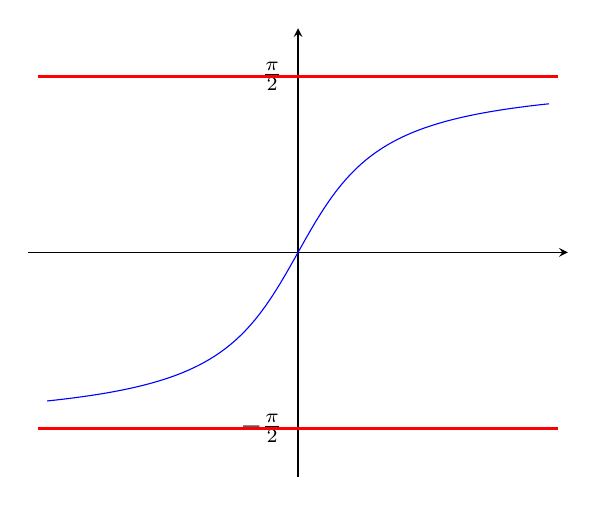
\begin{tikzpicture}
\begin{axis}[
  legend pos = north west,
  axis x line=center, axis y line=center,
  xmax=4.3,xmin=-4.3, xmajorticks=false,
  ymin=-2,ymax=2,
  ytick={-1.570796327,1.570796327},
  yticklabels={$-\frac{\pi}{2}$, $\frac{\pi}{2}$}
  ]
\addplot[blue,domain=-4:4,samples=100] {atan(x)/180*pi};
% \legend{$\tan \theta$}

\addplot[line width=1pt,red] coordinates {(4.15,-1.570796327) (-4.15,-1.570796327)};
\addplot[line width=1pt,red] coordinates {(4.15,1.570796327) (-4.15,1.570796327)};
\end{axis}
\end{tikzpicture}
\\ \hline
\end{tabular}
\renewcommand{\arraystretch}{1}
\end{center}
Since these functions are inverses of each other we have
\begin{align*}
  \arcsin(\sin \theta) &= \theta & -\frac{\pi}{2} \leq \theta \leq \frac{\pi}{2} \\
  \arccos(\cos \theta) &= \theta & 0 \leq \theta \leq \pi \\
  \arctan(\tan \theta) &= \theta & -\frac{\pi}{2} \leq \theta \leq \frac{\pi}{2}
\end{align*}
and also
\begin{align*}
  \sin(\arcsin x) &= x & -1 \leq x \leq 1 \\
  \cos(\arccos x) &= x & -1 \leq x \leq 1 \\
  \tan(\arctan x) &= x & \text{any real $x$}
\end{align*}
We can read other combinations of trig functions and their inverses, like, for
example, $\cos(\arcsin x)$, off of triangles like
\begin{efig}
\begin{center}
\includegraphics{../differentiation/triangleAsin}
\end{center}
\end{efig}
We have chosen the hypotenuse and opposite sides of the triangle
to be of length 1 and $x$, respectively, so that
$\sin(\theta)=x$. That is, $\theta =  \arcsin x$. We can then
read off of the triangle that
\begin{align*}
  \cos(\arcsin x) &= \cos(\theta) = \sqrt{1-x^2}
\end{align*}
We can reach the same conclusion using trig identities, as
follows.
\begin{itemize}
\item Write $\arcsin x=\theta$. We know that $\sin(\theta)=x$ and we wish to
compute $\cos(\theta)$. So we just need to express $\cos(\theta)$ in terms of
$\sin(\theta)$.

 \item To do this we make use of one of the Pythagorean identities
  \begin{align*}
  \sin^2\theta + \cos^2\theta &=1\\
  \cos\theta &= \pm \sqrt{1-\sin^2\theta}
\end{align*}
\item Thus
\begin{align*}
  \cos(\arcsin x) = \cos\theta = \pm\sqrt{1-\sin^2\theta}
\end{align*}

 \item To determine which branch we should use we need to consider the domain
and range of $\arcsin x$:
\begin{align*}
  \text{Domain: } -1 \leq x \leq 1 && \text{Range: } -\frac{\pi}{2} \leq \arcsin x \leq \frac{\pi}{2}
\end{align*}
  Thus we are applying cosine to an angle that always lies between $-\frac{\pi}{2}$ and $\frac{\pi}{2}$. Cosine is non-negative on this range. Hence we should take the positive branch and
\begin{align*}
  \cos(\arcsin x) &= \sqrt{1-\sin^2\theta}= \sqrt{1-\sin^2(\arcsin x)} \\
  &= \sqrt{1-x^2}
\end{align*}
\end{itemize}
In a very similar way we can simplify $\tan(\arccos x)$.
\begin{itemize}
\item Write $\arccos x=\theta$, and then
\begin{align*}
  \tan( \arccos x) &= \tan \theta = \frac{\sin\theta}{\cos \theta}
\end{align*}
\item Now the denominator is easy since $\cos \theta = \cos \arccos x = x$.
\item The numerator is almost the same as the previous computation.
\begin{align*}
  \sin\theta &= \pm \sqrt{1-\cos^2\theta} \\
  &= \pm \sqrt{1-x^2}
\end{align*}
 \item To determine which branch we again consider domains and
and ranges:
\begin{align*}
  \text{Domain: } -1 \leq x \leq 1 && \text{Range: } 0 \leq \arccos
x \leq \pi
\end{align*}
  Thus we are applying sine to an angle that always lies between
$0$ and $\pi$. Sine is non-negative on this range and so we take the positive
branch.
\item Putting everything back together gives
\begin{align*}
  \tan(\arccos x) &= \frac{\sqrt{1-x^2}}{x}
\end{align*}

\end{itemize}


Completing the 9 possibilities gives:
\begin{align*}
  \sin( \arcsin x ) &= x &
  \sin( \arccos x ) &= \sqrt{1-x^2} &
  \sin( \arctan x ) &= \frac{x}{\sqrt{1+x^2}} \\
%
  \cos( \arcsin x ) &= \sqrt{1-x^2} &
  \cos( \arccos x ) &= x &
  \cos( \arctan x ) &= \frac{1}{\sqrt{1+x^2}} \\
%
  \tan( \arcsin x ) &= \frac{x}{\sqrt{1-x^2}} &
  \tan( \arccos x ) &= \frac{\sqrt{1-x^2}}{x} &
  \tan( \arctan x ) &= x
\end{align*}

% \end{comment}

\section{Cosine and Sine Laws}\label{sec_B_4}
\subsection{Cosine Law or Law of Cosines}\label{app cosine law}
The cosine law says that, if a triangle has sides of length $a$, $b$ and $c$ and
the angle opposite the side of length $c$ is $\gamma$, then
\begin{align*}
  c^2 &= a^2+b^2 - 2ab\cos\gamma
\end{align*}
Observe that, when $\gamma=\tfrac{\pi}{2}$, this reduces to, (surpise!)
Pythagoras' theorem $c^2=a^2+b^2$. Let's derive the cosine law.
\begin{center}
 \includegraphics[height=3cm]{cosines}
\end{center}

Consider the triangle on the left. Now draw a perpendicular line from the side
of length $c$ to the opposite corner as shown. This demonstrates that
\begin{align*}
  c &= a \cos \beta + b \cos \alpha
\intertext{Multiply this by $c$ to get an expression for $c^2$:}
  c^2 &= ac \cos \beta + bc \cos \alpha
\intertext{Doing similarly for the other corners gives}
  a^2 &= ac \cos \beta + ab \cos \gamma \\
  b^2 &= bc \cos \alpha + ab \cos \gamma
\end{align*}
Now combining these:
\begin{align*}
  a^2+b^2-c^2 &=  (bc-bc) \cos \alpha + (ac-ac)\cos\beta + 2ab \cos \gamma \\
  &= 2ab\cos \gamma
\end{align*}
as required.

\subsection{Sine Law or Law of Sines}\label{ssec_B_4_2}
The sine law says that, if a triangle has sides of length $a, b$ and $c$ and
the angles opposite those sides are $\alpha$, $\beta$ and $\gamma$, then
\begin{align*}
  \frac{a}{\sin \alpha} &= \frac{b}{\sin \beta} = \frac{c}{\sin \gamma}.
\end{align*}
\begin{center}
 \includegraphics[height=3cm]{sines}
\end{center}
This rule is best understood by computing the area of the triangle using the
formula $A = \frac{1}{2}ab\sin\theta$ of Appendix~\ref{app sec areas}. Doing
this three ways gives
\begin{align*}
  2A &= bc \sin \alpha \\
  2A &= ac \sin \beta \\
  2A &= ab \sin \gamma
\end{align*}
Dividing these expressions by $abc$ gives
\begin{align*}
  \frac{2A}{abc} &= \frac{\sin \alpha}{a} = \frac{\sin\beta}{b} = \frac{\sin \gamma}{c}
\end{align*}
as required.

\section{Circles, cones and spheres}\label{sec_B_5}
\subsection{Where Does the Formula for the Area of a Circle Come From?}
\label{ssec_B_5_1}
Typically when we come across $\pi$ for the first time it is as the ratio of the
circumference of a circle to its diameter
\begin{align*}
  \pi &= \frac{C}{d} = \frac{C}{2r}
\end{align*}
Indeed this is typically the first definition we see of $\pi$.  It is easy to build an intuition that the area of the circle should be propotional to the square of its radius. For example we can draw the largest possible square inside the circle (an \emph{inscribed} square) and the smallest possible square outside the circle (a \emph{circumscribed} square):
\begin{center}
 \includegraphics[height=35mm]{archimedes0}
\end{center}
The smaller square has side-length $\sqrt{2} r$ and the longer has side-length $2r$. Hence
\begin{align*}
  2 r^2 & \leq A \leq 4r^2 & \text{ or }  2 & \leq \frac{A}{r^2} \leq 4
\end{align*}
That is, the area of the circle is between 2 and 4 times the square of the radius. What is perhaps less obvious (if we had not been told this in school) is that the constant of propotionality for area is also $\pi$:
\begin{align*}
  \pi &= \frac{A}{r^2}.
\end{align*}


We will show this using Archimedes' proof. He makes use of these inscribed and circumscribed polygons to make better and better approximations of the circle. The steps of the proof are somewhat involved and the starting point is to rewrite the area of a circle as
\begin{align*}
  A &= \frac{1}{2} C r
\end{align*}
where $C$ is (still) the circumference of the circle. This suggests that this
area is the same as that of a triangle of height $r$ and base
length $C$
\begin{align*}
  T &= \frac{1}{2} C r
\end{align*}
\begin{center}
 \includegraphics[height=3cm]{archimedes1}
\end{center}
Archimedes' proof then demonstrates that indeed this triangle and the circle have the same
area. It relies on a ``proof by contradiction'' --- showing that $T<A$ and $T>A$ cannot
be true and so the only possibility is that $A=T$.

We will first show that $T<A$ cannot happen. Construct an $n$-sided ``inscribed'' polygon
as shown below:
\begin{center}
 \includegraphics[height=4cm]{archimedes2}
\end{center}
Let $p_n$ be the inscribed polygon as shown.
\begin{center}
 \includegraphics[width=\textwidth]{archimedes3}
\end{center}
We need 4 steps.
\begin{enumerate}
 \item The area of $p_n$ is smaller than that of the circle --- this follows since we can
construct $p_n$ by cutting slices from the circle.
 \item Let $E_n$ be the difference between the area of the circle and $p_n$: $E_n = A -
A(p_n)$ (see the left of the previous figure). By the previous point we know $E_n>0$.
Now as we increase the number of sides, this difference becomes smaller. To be more
precise
  \begin{align*}
  E_{2n} & \leq \frac{1}{2} E_n.
  \end{align*}
The error $E_n$ is made up of $n$ ``lobes''. In the centre-left of the previous figure we
draw one such lobe and surround it by a rectangle of dimensions $a \times 2b$ --- we
could determine these more precisely using a little trigonometry, but it is not necessary.

This diagram shows the lobe is smaller than the rectangle of base $2b$ and height $a$
Since there are $n$ copies of the lobe, we have
\begin{align*}
  E_n & \leq n  \times 2ab & \text{rewrite as } \frac{E_n}{2} & \leq nab
\end{align*}

Now draw in the polygon $p_{2n}$ and consider the associated ``error'' $E_{2n}$. If we
focus on the two lobes shown then we see that the area of these two new lobes is equal to
that of the old lobe (shown in centre-left) minus the area of the triangle with base $2b$
and height $a$ (drawn in purple). Since there are $n$ copies of this
picture we have
\begin{align*}
  E_{2n} &= E_n - nab & \text{now use that $nab \geq  E_n/2$} \\
  & \leq E_n - \frac{E_n}{2} = \frac{E_n}{2}
\end{align*}

\item The area of $p_n$ is smaller than $T$. To see this decompose $p_n$ into $n$
isosceles triangles. Each of these has base shorter than $C/n$; the straight line is
shorter than the corresponding arc --- though strictly speaking we should prove this. The
height of each triangle is shorter than $r$. Thus
\begin{align*}
  A(p_n) &= n \times \frac{1}{2} \text{(base)}\times \text{(height)} \\
  & \leq n \times \frac{Cr}{2n} = T
\end{align*}

\item If we assume that $T<A$, then $A-T = d$ where $d$ is some positive number.
However we know from point 2 that we can make $n$ large enough so that $E_n < d$
(each time we double $n$ we halve the error). But now we have a contradiction to
step~3, since we have just shown that
\begin{align*}
  E_n = A-A(p_n) & < A-T & \text{which implies that}\\
  A(p_n) & > T.
\end{align*}
\end{enumerate}
Thus we cannot have $T<A$.

If we now assume that $T>A$ we will get a similar contradiction by a similar
construction. Now we use regular $n$-sided \emph{circumscribed} polygons, $P_n$.
\begin{center}
 \includegraphics[height=35mm]{archimedes4}
\end{center}
The proof can be broken into 4 similar steps.
\begin{center}
 \includegraphics[width=\textwidth]{archimedes5}
\end{center}
\begin{enumerate}
 \item The area of $P_n$ is greater than that of the circle --- this follows since we
can construct the circle by trimming the polygon $P_n$.

 \item Let $E_n$ be the difference between the area of the polygon and the circle: $E_n =
A(P_n)-A$ (see the left of the previous figure). By the previous point we know $E_n>0$.
Now as we increase the number of sides, this difference becomes smaller. To be more
precise we will show
  \begin{align*}
  E_{2n} & \leq \frac{1}{2} E_n.
  \end{align*}
The error $E_n$ is made up of $n$ ``lobes''. In the centre-left of the previous figure we
draw one such lobe. Let $L_n$ denote the area of one of these lobes, so $E_n = nL_n$.  In
the centre of the previous figure we have labelled this lobe carefully and also shown how
it changes when we create the polygon $P_{2n}$. In particular, the original lobe is
bounded by the straight lines $\vec{ad}, \vec{af}$ and the arc $\widehat{fbd}$. We create
$P_{2n}$ from $P_n$ by cutting away the corner triangle $\triangle aec$. Accordingly the
lines $\vec{ec}$ and $\vec{ba}$ are orthogonal and the segments $|bc|=|cd|$.

By the construction of $P_{2n}$ from $P_n$, we have
\begin{align*}
  2L_{2n} &= L_n - A( \triangle aec) & \text{or equivalently }
  L_{2n} &= \frac{1}{2} L_n - A( \triangle abc)
\end{align*}
And additionally
\begin{align*}
  L_{2n} & \leq A( \triangle bcd)
\end{align*}

Now consider the triangle $\triangle abd$ (centre-right of the previous figure) and the
two triangles within it $\triangle abc$ and $\triangle bcd$. We know that $\vec{ab}$ and
$\vec{cb}$ form a right-angle. Consequently $\vec{ac}$ is the hypotenuse of a right-angled
triangle, so $|ac|>|bc| = |cd|$. So now, the triangles $\triangle abc$ and $\triangle bcd$
have the same heights, but the base of $\vec{ac}$ is longer than $\vec{cd}$. Hence the
area of $\triangle abc$ is strictly larger than that of $\triangle bcd$.

Thus we have
\begin{align*}
  L_{2n} & \leq A(\triangle bcd) < A(\triangle abc)
\end{align*}
But now we can write
\begin{align*}
  L_{2n} &= \frac{1}{2} L_n - A( \triangle abc) < \frac{1}{2} L_n - L_{2n}  &
\text{rearrange}\\
  2L_{2n} &< \frac{1}{2} L_n & \text{there are $n$ such lobes, so } \\
  2n L_{2n} &< \frac{n}{2} L_n & \text{since $E_n = n L_n$, we have}\\
  E_{2n} & < \frac{1}{2} E_n & \text{which is what we wanted to show.}
\end{align*}


\item The area of $P_n$ is greater than $T$. To see this decompose $P_n$ into $n$
isosceles triangles. The height of each triangle is $r$, while the base of each is longer
than $C/n$ (this is a subtle point and its proof is equivalent to showing that $\tan
\theta > \theta$). Thus
\begin{align*}
  A(P_n) &= n \times \frac{1}{2} \text{(base)}\times \text{(height)} \\
  & \geq n \times \frac{Cr}{2n} = T
\end{align*}

\item If we assume that $T>A$, then $T-A = d$ where $d$ is some positive number.
However we know from point 2 that we can make $n$ large enough so that $E_n < d$ (each
time we double $n$ we halve the error). But now we have a contradiction since we have just
shown that
\begin{align*}
  E_n = A(P_n) - A & < T-A & \text{which implies that}\\
  A(p_n) & > T.
\end{align*}
\end{enumerate}
Thus we cannot have $T>A$. The only possibility that remains is that $T=A$.


\subsection{Where Do These Volume Formulas Come From?}\label{apendix volume}
We can establish the volumes of cones and spheres from the formula for the volume of a
cylinder and a little work with limits and some careful summations. We first need a few
facts.
\begin{itemize}
 \item Every square number can be written as a sum of consecutive odd numbers. More
precisely
  \begin{align*}
  n^2 &= 1 + 3 + \dots (2n-1)
\end{align*}
 \item The sum of the first $n$ positive integers is $\frac{1}{2} n(n+1)$. That is
\begin{align*}
  1 + 2 +3 +\dots +n &= \frac{1}{2}n(n+1)
\end{align*}
 \item The sum of the squares of the first $n$ positive integers is $\frac{1}{6}
n(n+1)(2n+1)$.
\begin{align*}
  1^2 + 2^2 +3^2 +\dots + n^2 &= \frac{1}{6}n(n+1)(2n+1)
\end{align*}
\end{itemize}
We will not give completely rigorous proofs of the above identities (since we are not
going to assume that the reader knows mathematical induction), rather we will explain
them using pictorial arguments. The first two of these we can explain by some quite simple
pictures:
\begin{center}
 \includegraphics[width=\textwidth]{sums1}
\end{center}
We see that we can decompose any square of unit-squares into a sequence of strips, each
of which consists of an odd number of unit-squares. This is really just from the fact that
\begin{align*}
  n^2 - (n-1)^2 &= 2n-1
\end{align*}
Similarly, we can represent the sum of the first $n$ integers as a triangle of unit
squares as shown. If we make a second copy of that triangle and arrange it as shown, it
gives a rectangle of dimensions $n$ by $n+1$. Hence the rectangle, being exactly twice the
size of the original triangle, contains $n(n+1)$ unit squares.

The explanation of the last formula takes a little more work and a carefully
constructed picture:
\begin{center}
 \includegraphics[width=\textwidth]{sums2}
\end{center}
Let us break these pictures down step by step
\begin{itemize}
 \item Leftmost represents the sum of the squares of the first $n$ integers.
 \item Centre --- We recall from above that each square number can be written as a sum of
consecutive odd numbers, which have been represented as coloured bands of unit-squares.
 \item Make three copies of the sum and arrange them carefully as shown. The first and
third copies are obvious, but the central copy is rearranged considerably; all
bands of the same colour have the same length and have been arranged into
rectangles as shown.

Putting everything from the three copies together creates a rectangle of dimensions
$(2n+1)\times(1+2+3+\dots+n)$.
\end{itemize}
We know (from above) that $1+2+3+\dots+n = \frac{1}{2} n(n+1)$ and so
\begin{align*}
  (1^2+2^2+\dots+n^2 ) &= \frac{1}{3} \times \frac{1}{2} n(n+1)(2n+1)
\end{align*}
as required.

Now we can start to look at volumes. Let us start with the volume of a cone; consider the
figure below. We bound the volume of the cone above and below by stacks of cylinders. The
cross-sections of the cylinders and cone are also shown.
\begin{center}
 \includegraphics[width=0.8\textwidth]{cone}
\end{center}
To obtain the bounds we will construct two stacks of $n$ cylinders, $C_1,C_2,\dots,C_n$.
Each cylinder has height $h/n$ and radius that varies with height. In particular, we
define cylinder $C_k$ to have height $h/n$ and radius $k \times r/n$. This radius was
determined using similar triangles so that cylinder $C_n$ has radius $r$. Now cylinder
$C_k$ has volume
\begin{align*}
  V_k &= \pi \times \text{radius}^2 \times \text{height}
  = \pi \left( \frac{kr}{n} \right)^2 \cdot \frac{h}{n}\\
  &= \frac{\pi r^2h}{n^3} k^2
\end{align*}

We obtain an upper bound by stacking cylinders $C_1,C_2,\dots,C_n$ as shown. This object
has volume
\begin{align*}
  V &= V_1 + V_2 + \dots V_n \\
  &= \frac{\pi r^2h}{n^3} \left(1^2 + 2^2 + 3^2 + \dots + n^2 \right) \\
  &= \frac{\pi r^2h}{n^3} \cdot \frac{n(n+1)(2n+1)}{6}
\end{align*}
A similar lower bound is obtained by stacking cylinders $C_1,\dots,C_{n-1}$ which gives a
volume of
\begin{align*}
  V &= V_1 + V_2 + \dots V_{n-1} \\
  &= \frac{\pi r^2h}{n^3} \left(1^2 + 2^2 + 3^2 + \dots + (n-1)^2 \right) \\
  &= \frac{\pi r^2h}{n^3} \cdot \frac{(n-1)(n)(2n-1)}{6}
\end{align*}
Thus the true volume of the cylinder is bounded between
\begin{align*}
  \frac{\pi r^2h}{n^3} \cdot \frac{(n-1)(n)(2n-1)}{6}
  & \leq \text{correct volume}
  \leq \frac{\pi r^2h}{n^3} \cdot \frac{n(n+1)(2n+1)}{6}
\end{align*}
We can now take the limit as the number of cylinders, $n$, goes to infinity. The upper
bound becomes
\begin{align*}
  \lim_{n \to \infty} \frac{\pi r^2h}{n^3} \frac{n(n+1)(2n+1)}{6}
  &= \frac{\pi r^2h}{6} \lim_{n\to\infty} \frac{n(n+1)(2n+1)}{n^3} \\
  &= \frac{\pi r^2h}{6} \lim_{n\to\infty} \frac{(1+1/n)(2+1/n)}{1} \\
  &= \frac{\pi r^2h}{6} \times 2 \\
  &= \frac{\pi r^2h}{3}
\end{align*}
The other limit is identical, so by the squeeze theorem we have
\begin{align*}
  \text{Volume of cone } &= \frac{1}{3} \pi r^2h
\end{align*}

Now the sphere --- though we will do the analysis for a hemisphere of radius $R$. Again
we bound the volume above and below by stacks of cylinders. The cross-sections of the
cylinders and cone are also shown.
\begin{center}
 \includegraphics[width=0.8\textwidth]{sphere}
\end{center}
To obtain the bounds we will construct two stacks of $n$ cylinders, $C_1,C_2,\dots,C_n$.
Each cylinder has height $R/n$ and radius that varies with its position in the
stack. To describe the position, define
\begin{align*}
  y_k &= k \times \frac{R}{n}
\end{align*}
That is, $y_k$, is $k$ steps of distance $\frac{R}{n}$ from the top of the
hemisphere. Then we set the $k^\mathrm{th}$ cylinder, $C_k$ to have height $R/n$
and radius $r_k$ given by
\begin{align*}
  r_k^2 &= R^2 - (R-y_k)^2 = R^2 - R^2(1-k/n)^2 \\
  &= R^2( 2k/n - k^2/n^2)
\end{align*}
as shown in the top-right and bottom-left illustrations. The volume of $C_k$ is then
\begin{align*}
  V_k &= \pi \times \text{radius}^2 \times \text{height}
  = \pi \times R^2 \left(2k/n - k^2/n^2  \right) \times \frac{R}{n}\\
  &=  \pi R^3 \cdot \left( \frac{2k}{n^2}  - \frac{k^2}{n^3} \right)
\end{align*}

We obtain an upper bound by stacking cylinders $C_1,C_2,\dots,C_n$ as shown. This object
has volume
\begin{align*}
  V &= V_1 + V_2 + \dots V_n \\
  &=
\pi R^3 \cdot \left( \frac{2}{n^2}\left(1 + 2 + 3 + \dots + n \right)
- \frac{1}{n^3}\left(1^2 + 2^2 + 3^2 + \dots + n^2 \right) \right)
\end{align*}
Now recall from above that
\begin{align*}
  1 + 2 + 3 + \dots +n &= \frac{1}{2} n(n+1) &
  1^2 + 2^2 + 3^2 + \dots +n^2 &= \frac{1}{6} n(n+1)(2n+1)
\end{align*}
so
\begin{align*}
  V &= \pi R^3 \cdot \left( \frac{n(n+1)}{n^2}
- \frac{n(n+1)(2n+1)}{6n^3} \right)
\end{align*}

Again, a lower bound is obtained by stacking cylinders $C_1,\dots,C_{n-1}$ and a similar
analysis gives
\begin{align*}
  V &= \pi R^3 \cdot \left( \frac{n(n-1)}{(n-1)^2}
- \frac{n(n-1)(2n-1)}{6(n-1)^3} \right)
\end{align*}

Thus the true volume of the hemisphere is bounded between
\begin{align*}
  \pi R^3 \cdot \left( \frac{n(n+1)}{n^2}
- \frac{n(n+1)(2n+1)}{6n^3} \right)
  & \leq \text{correct volume}
  \leq \pi R^3 \cdot \left( \frac{n(n+1)}{n^2}
- \frac{n(n+1)(2n+1)}{6n^3} \right)
\end{align*}
We can now take the limit as the number of cylinders, $n$, goes to infinity. The upper
bound becomes
\begin{align*}
  \lim_{n \to \infty} \pi R^3 \cdot \left( \frac{n(n+1)}{n^2}
- \frac{n(n+1)(2n+1)}{6n^3} \right)
  &= \pi R^3 \left( \lim_{n\to\infty} \frac{n(n+1)}{n^2} -
\frac{n(n+1)(2n+1)}{6n^3}
\right)\\
  &= \pi R^3 \left( 1 - \frac{2}{6} \right) = \frac{2}{3} \pi R^3.
\end{align*}
The other limit is identical, so by the squeeze theorem we have
\begin{align*}
  \text{Volume of hemisphere } &= \frac{2}{3} \pi R^3 & \text{ and so}\\
  \text{Volume of sphere } &= \frac{4}{3} \pi R^3
\end{align*}


\end{document}
